% Current Q--DESN vector figures are PDF 1.7.  Match their version so pdfTeX
% embeds them without silently accepting a newer object format than advertised.
\ifdefined\pdfminorversion\pdfminorversion=7\fi
\documentclass[12pt,oneside,final,dissertation]{ucscthesis}
% Identity supplied by the author on 2026-09-15. The Dissertation Reading
% Committee below was approved by Graduate Division and updated in AIS on
% 2026-10-09; Statistics Graduate Advising forwarded confirmation on
% 2026-10-12. Remaining title, date, dean, and signature fields are unresolved.
\newcommand{\ThesisTitle}{[Dissertation title to be confirmed]}
\newcommand{\AuthorName}{Jose Antonio Aguirre Perez de Leon}
% Use "Antonio de Leon" as the scholarly name in new dissertation prose and
% contribution records. Preserve source spellings in immutable citations.
\newcommand{\ScholarlyName}{Antonio de Leon}
\newcommand{\DegreeName}{DOCTOR OF PHILOSOPHY}
\newcommand{\DegreeField}{STATISTICAL SCIENCE} % Verify against MyUCSC record.
\newcommand{\DegreeMonth}{[Conferral month]} % Fall -> December, if confirmed.
\newcommand{\DegreeYear}{[Conferral year]}
% Approved Dissertation Reading Committee; the nomination form specifies that
% the chair is listed first, and advising separately confirmed Raquel Prado's
% chair role.
\newcommand{\CommitteeOne}{Raquel Prado, Chair}
\newcommand{\CommitteeTwo}{Bruno Sans\'o}
\newcommand{\CommitteeThree}{Paul Parker}
\newcommand{\CommitteeFour}{Athanasios Kottas}
\newcommand{\DeanName}{[Current dean: confirm]}
\newcommand{\DeanTitle}{[Exact dean title: confirm]}
\newif\ifStarterDraft
\StarterDrafttrue % Retain until the remaining formal fields and approval are final.
\title{\ThesisTitle}
\author{\AuthorName}
\degree{\DegreeName}
\field{\DegreeField}
\campus{SANTA CRUZ}
\degreemonth{\DegreeMonth}
\degreeyear{\DegreeYear}

% University guide G1, pp. 2-8; mapping in docs/compliance-matrix.md.
\usepackage[T1]{fontenc}
\usepackage[utf8]{inputenc}
% Older pdfTeX releases do not always emit ToUnicode maps by default.
\ifdefined\pdfgentounicode
  \input{glyphtounicode}
  \pdfgentounicode=1
\fi
% Broadly available Times-compatible Type 1 text/math; all actual fonts checked.
\usepackage{mathptmx}
\usepackage{amsmath,amssymb,amsthm,mathtools,bm}
% Small vertical clearance keeps visible glyph bounds inside the 1.25 in minimum.
\usepackage[letterpaper,left=1.5in,right=1.25in,top=1.30in,bottom=1.35in,
  headheight=0pt,headsep=0pt,footskip=0.4in]{geometry}
% Legacy class does not initialize setspace's current-size hook.
\makeatletter
\let\@currsize\normalsize
\makeatother
\usepackage{setspace}
% The legacy class uses 1.37; override it instead of relying on its name.
% At 12 pt, setspace double spacing gives approximately 24 pt baseline distance.
\renewcommand{\dsp}{\doublespacing}
\renewcommand{\ssp}{\singlespacing}
\AtBeginDocument{\doublespacing}
\setlength{\parindent}{0.3in}
\setlength{\parskip}{0pt}
\raggedbottom
\usepackage{fancyhdr}
\pagestyle{fancy}
\fancyhf{}
% Asymmetric margins shift the text centre right by 0.125 in.
% Extend footer 0.25 in left to centre the number on the physical sheet.
\fancyfootoffset[L]{0.25in}
\fancyfoot[C]{\normalsize\thepage}
\renewcommand{\headrulewidth}{0pt}
\renewcommand{\footrulewidth}{0pt}
\fancypagestyle{plain}{\fancyhf{}\fancyfoot[C]{\normalsize\thepage}
  \renewcommand{\headrulewidth}{0pt}\renewcommand{\footrulewidth}{0pt}}
\usepackage{graphicx,booktabs,array,tabularx,float,enumitem,longtable,xcolor,etoolbox}
\usepackage{tikz}
\usetikzlibrary{arrows.meta,calc,fit,positioning}
\usepackage{algorithm,algorithmic}
\usepackage[font=normalsize,labelfont=bf]{caption}
\captionsetup{singlelinecheck=false,justification=justified}
% Article floats were designed for single-spaced journal pages.  Keep tables,
% figures, and algorithms single-spaced inside the otherwise double-spaced
% dissertation, as permitted exceptions.  Font size is selected locally for
% each display rather than imposed on every table or algorithm.
\AtBeginEnvironment{table}{\singlespacing}
\AtBeginEnvironment{figure}{\singlespacing}
\AtBeginEnvironment{algorithm}{\singlespacing}
\AtBeginEnvironment{algorithmic}{\singlespacing\small}
\AtBeginEnvironment{longtable}{\singlespacing}
\setlength{\emergencystretch}{2em}
\allowdisplaybreaks
% natbib renews a command the legacy class defines only inside its own list.
\providecommand{\newblock}{}
\usepackage[authoryear,round]{natbib}
\setlength{\bibsep}{11.5pt} % Single within, near-baseline separation between entries.
\renewcommand{\bibfont}{\singlespacing\normalsize}
\renewcommand{\bibsection}{\chapter*{Bibliography}
  \addcontentsline{toc}{chapter}{Bibliography}}
\usepackage{url}
\urlstyle{same}
\usepackage[hidelinks,bookmarksnumbered,pdfpagelabels]{hyperref}
\hypersetup{pdftitle={\ThesisTitle},pdfauthor={\AuthorName},
 pdfsubject={Dissertation in Statistical Science}}
\newtheorem{theorem}{Theorem}[chapter]
\newtheorem{proposition}{Proposition}[chapter]
\newtheorem{lemma}{Lemma}[chapter]
\newtheorem{corollary}{Corollary}[chapter]
\theoremstyle{definition}
\newcounter{thesisalgorithm}[chapter]
\renewcommand{\thethesisalgorithm}{\thechapter.\arabic{thesisalgorithm}}
\newenvironment{algorithmblock}[1]{%
  \refstepcounter{thesisalgorithm}%
  \par\medskip\noindent\textbf{Algorithm~\thethesisalgorithm. #1.}\par\nobreak
}{\par\medskip}
% The server TeX installation lacks threeparttable.  These compatible wrappers
% retain its manuscript table bodies and notes without introducing a package
% dependency or reducing the dissertation text size.
\newenvironment{threeparttable}{}{}
\newenvironment{tablenotes}{%
  \begin{list}{}{\setlength{\leftmargin}{0.2in}\setlength{\itemsep}{0pt}}%
}{\end{list}}
\providecommand{\FloatBarrier}{}
\providecommand{\pkg}[1]{\textsf{#1}}
\providecommand{\proglang}[1]{\textsf{#1}}
\providecommand{\code}[1]{\texttt{\detokenize{#1}}}
\providecommand{\figalt}[1]{}
\newcolumntype{Y}{>{\raggedright\arraybackslash}X}
\providecommand{\tworowcell}[1]{\smash{\raisebox{-0.5\normalbaselineskip}{#1}}}
\providecommand{\TableStyle}{\small\setlength{\tabcolsep}{4pt}%
  \renewcommand{\arraystretch}{1.08}}
\providecommand{\CompactTableStyle}{\scriptsize\setlength{\tabcolsep}{2.3pt}%
  \renewcommand{\arraystretch}{1.0}}
\newcommand{\DemoNotice}{\par\noindent\textbf{Formatting demonstration only.}
 This material is not the candidate's research.\par}
% Preserve 12 pt footnote text. Superscript marks and mathematical scripts
% naturally use reduced sizes; no primary text is deliberately reduced.
\makeatletter
\renewcommand\footnotesize{\@setfontsize\footnotesize{12}{14.5}}
\makeatother
\AtBeginDocument{\typeout{UCSC-CHECK textwidth=\the\textwidth;
 textheight=\the\textheight; baseline=\the\baselineskip;
 oddsidemargin=\the\oddsidemargin; footskip=\the\footskip}}

% Project-wide notation. Audit article macros before extending this file.
\newcommand{\R}{\mathbb{R}}
\newcommand{\E}{\mathbb{E}}
\newcommand{\Prob}{\mathbb{P}}
\newcommand{\given}{\,\vert\,}
\providecommand{\vect}[1]{\boldsymbol{#1}}
\providecommand{\mat}[1]{\mathbf{#1}}
\providecommand{\N}{\mathcal{N}}
\providecommand{\Normal}{\mathcal{N}}
\providecommand{\TN}{\mathcal{N}^{+}}
\providecommand{\TNp}{\mathcal{N}^{+}}
\providecommand{\IG}{\operatorname{IG}}
\providecommand{\GIG}{\operatorname{GIG}}
\providecommand{\Exp}{\operatorname{Exp}}
\providecommand{\Unif}{\operatorname{Unif}}
\providecommand{\AL}{\operatorname{AL}}
\providecommand{\exAL}{\operatorname{exAL}}
\providecommand{\KL}{\operatorname{KL}}
\providecommand{\CRPS}{\operatorname{CRPS}}
\providecommand{\PPLC}{\operatorname{PPLC}}
\providecommand{\RHS}{\ensuremath{\operatorname{RHS}}}
\providecommand{\aCRPS}{\operatorname{aCRPS}}
\providecommand{\StudentT}{\operatorname{t}}
\providecommand{\Rp}{\mathbb{R}_{+}}
\providecommand{\Ind}{\mathbb{I}}
\providecommand{\ind}{\mathbf{1}}
\providecommand{\Var}{\operatorname{Var}}
\providecommand{\Cov}{\operatorname{Cov}}
\providecommand{\tr}{\operatorname{tr}}
\providecommand{\diag}{\operatorname{diag}}
\providecommand{\logit}{\operatorname{logit}}
\providecommand{\expit}{\operatorname{expit}}
\providecommand{\elbo}{\mathcal{L}}
\providecommand{\pigamma}{\pi_\gamma}
\providecommand{\Id}[1]{\mat I_{#1}}
\providecommand{\zeros}[1]{\vect 0_{#1}}
\providecommand{\ones}[1]{\vect 1_{#1}}
\providecommand{\argmin}{\operatorname*{arg\,min}}

\begin{document}
\pagenumbering{roman}
% Adapted layout from ucscthesis.cls; original class remains unchanged.
% G1 sample p. 10. Integrated unsigned approval block; no extra numbered page.
\thispagestyle{empty}
\begin{singlespace}
\begin{center}
UNIVERSITY OF CALIFORNIA\par\smallskip
SANTA CRUZ\par\bigskip
\textbf{\MakeUppercase{\ThesisTitle}}\par\bigskip
A dissertation submitted in partial satisfaction of the\par
requirements for the degree of\par\bigskip
\DegreeName\par\bigskip
in\par\bigskip
\DegreeField\par\bigskip
by\par\bigskip
\textbf{\AuthorName}\par\bigskip
\DegreeMonth\ \DegreeYear\par
\ifStarterDraft\bigskip\textbf{FORMATTING STARTER}\par
Not for submission; dissertation approval and remaining formal fields are
unresolved.\par\fi
\end{center}
\vfill
\noindent\hfill\begin{minipage}{3.0in}
\ifStarterDraft
Dissertation Reading Committee:
\else
The Dissertation of \AuthorName\ is approved:
\fi
\par\medskip
\rule{\linewidth}{0.4pt}\par\CommitteeOne\par\medskip
\rule{\linewidth}{0.4pt}\par\CommitteeTwo\par\medskip
\rule{\linewidth}{0.4pt}\par\CommitteeThree\par\medskip
\rule{\linewidth}{0.4pt}\par\CommitteeFour\par
\end{minipage}
\par\bigskip
\noindent\begin{minipage}{3.0in}
\rule{\linewidth}{0.4pt}\par\DeanName\par\DeanTitle
\end{minipage}
\end{singlespace}
\clearpage

% Author-selected copyright notice in the current UCSC sample format. This is
% the unnumbered, counted page ii; copyright registration remains a separate
% optional ProQuest decision.
\thispagestyle{empty}
\null
\vfill
\begin{center}
Copyright \textcopyright\par
by \AuthorName\par
\DegreeYear
\end{center}
\vfill
\null
\clearpage

\tableofcontents
\listoffigures
\listoftables
\begin{abstract}
This dissertation studies statistical inference for conditional quantiles and
fixed-content intervals when temporal dependence, nonlinear structure,
heterogeneous forecast products, and computational constraints complicate full
response-distribution modeling. The central approach is target-first: the
inferential object, information set, update, and validation claim are specified
separately so that fitted quantiles, posterior predictive distributions,
endpoint uncertainty, and tolerance intervals are not conflated.

The first contribution is the \pkg{exdqlm} \proglang{R} package for extended
dynamic quantile linear models. It connects composable state-space models with
MCMC and variational inference, diagnostics, forecasting, post-fit predictive
synthesis, and static shrinkage regression. The second contribution applies
dynamic quantile models to source-aware correction and synthesis of river-flow
products. In a five-origin San Lorenzo River study, the selected multivariate
extended-asymmetric-Laplace specification gives the strongest 28-day comparison
among the evaluated Bayesian variants, while the common eight-day comparison
shows that gains are not uniform across every origin and horizon.

The third contribution develops Bayesian quantile deep echo-state networks,
which combine fixed nonlinear recurrent features with single-level or joint
quantile regression. MCMC and model-specific variational methods are examined
through simulations and retrospective GloFAS and PriceFM applications. The
multiquantile model reduces crossing without a uniform score gain. At one
GloFAS forecast origin, Q--DESN improves the reported quantile score over the
raw ensemble but its nominal interval remains undercovered; across 114 matched
PriceFM comparisons, each method wins in a substantial fraction of cases. The
fourth contribution studies mean-tilted intervals, a family of contiguous
fixed-content targets indexed by retained-mean balance. It characterizes the
mean-preserving member and develops a calibrated profiled MTI tolerance
procedure that screens fitted content and tilt using a direct posterior content
check. Independent simulations support the procedure on a fixed
eight-distribution panel, and a pharmaceutical application illustrates its
placement behavior and data limitations. Regression and dynamic endpoint
formulations are derived as proposed extensions.

Across the four projects, conditionally Gaussian representations make posterior
simulation and variational approximation practical, but similar computation
does not imply identical inference. Asymmetric-Laplace working likelihoods,
generalized posteriors for loss-defined endpoints, predictive synthesis, and
repeated-sampling tolerance calibration support different claims. Together,
the studies illustrate how distributional targets can be modeled and evaluated
without erasing those distinctions, and they identify the additional theory and
multi-origin validation required for broader predictive and tolerance claims.
\end{abstract}

% Optional acknowledgments are omitted until author-approved text is available.
\clearpage
\pagenumbering{arabic}
\chapter{Introduction and common framework}
\label{ch:introduction}

\section{Research problem and scope}
\label{sec:intro-problem}

Statistical decisions often depend on features of a conditional distribution
that are not summarized by its mean. A flood forecast may require upper-tail
quantiles, a manufacturing analysis may require an interval containing a fixed
fraction of a population, and a time-series analysis may require these targets
to change with recent information. In each case, the inferential object must be
specified before a model, computational method, or validation criterion can be
chosen. A fitted conditional quantile, a posterior predictive distribution, a
random interval for an unknown parameter, and a tolerance interval are distinct
objects even when they are displayed using similar endpoints.

This dissertation studies the following question:

\begin{quote}
How can conditional quantiles and fixed-content interval targets be specified,
computed, and validated when dynamics, nonlinear structure, heterogeneous
forecast products, and practical computational constraints make full
response-distribution modeling difficult or undesirable?
\end{quote}

The four research chapters address different parts of this question. The first
develops statistical software for established extended dynamic quantile linear
models. The second uses those models to correct and synthesize heterogeneous
hydrologic products. The third combines fixed nonlinear recurrent features with
Bayesian quantile regression. The fourth studies fixed-content interval
placement, a calibrated empirical tolerance action, and proposed regression and
dynamic endpoint extensions. The chapters share an emphasis on distributional
features, but they do not share one probability model or one interpretation of
uncertainty. Their connection instead lies in a common discipline: identify the
target, state what information defines it, choose an update and dependence
representation suited to that target, and validate the resulting claim at the
same inferential level.

This chapter establishes that common framework. It first distinguishes
conditional quantiles from fixed-content intervals. It then separates ordinary
likelihood-based Bayes from generalized updating and describes the dependence
representations and computational strategies used in the research chapters.
The final sections state the evidence boundaries, locate the jointly authored
project contributions relative to their antecedents, and describe the
organization of the dissertation.

\section{Conditional quantiles and fixed-content intervals}
\label{sec:intro-targets}

Let $Y$ denote a response and let $\mathcal F$ denote the information available
when an inferential target is defined. For $0<\tau<1$, the conditional
$\tau$-quantile is
\begin{equation}
Q_\tau(Y\mid\mathcal F)
=\inf\{q:\Pr(Y\le q\mid\mathcal F)\ge\tau\}.
\label{eq:intro-conditional-quantile}
\end{equation}
It minimizes the conditional expected check loss
\begin{equation}
\rho_\tau(u)=u\{\tau-\Ind(u<0)\},
\qquad
Q_\tau(Y\mid\mathcal F)
\in\argmin_q\E\{\rho_\tau(Y-q)\mid\mathcal F\},
\label{eq:intro-check-loss}
\end{equation}
under the usual regularity and uniqueness conditions
\citep{qdesn-KoenkerBassett1978,qdesn-Koenker2005}. Quantile regression models
the response at selected probability levels without requiring a complete
parametric description of its conditional distribution. In a time series,
$\mathcal F$ may include past responses, latent states, observed covariates, or
forecast-origin information. The conditioning set is therefore part of the
target rather than an incidental modeling detail.

Multiple fitted quantiles provide more distributional information than one
conditional mean, but a collection of separate fits is not automatically a
joint response-distribution model. Quantiles fitted independently may cross,
and uncertainty obtained within one fit does not by itself describe dependence
across probability levels. Monotone rearrangement can enforce an ordered curve
after fitting \citep{qdesn-BarlowBrunk1972IsotonicDual,exd-chernozhukov2010},
while a joint model may introduce explicit dependence or shrinkage across the
quantile index. These operations answer different questions and are identified
separately in Chapters~\ref{ch:research-a}--\ref{ch:research-c}.

A fixed-content interval begins from another target. For a continuous
distribution $F$ and prescribed content $c\in(0,1)$, many intervals
$[a,b]$ can satisfy
\begin{equation}
F(b)-F(a)=c.
\label{eq:intro-fixed-content}
\end{equation}
Content alone does not determine placement. Equal-tailed, shortest-contiguous,
and mean-preserving intervals impose different placement criteria and generally
have different endpoints for an asymmetric distribution. Chapter~\ref{ch:research-d}
uses retained-mean balance to index a family of such targets. Although an
equal-tailed interval can be formed from two quantiles, the general
fixed-content problem cannot be reduced to fitting a predetermined pair of
quantile levels.

The distinction becomes sharper for tolerance inference. If a data-dependent
interval $[L(\mathcal D),U(\mathcal D)]$ is intended to contain at least a
fraction $c$ of the population with confidence $1-\alpha$, the claim is
\begin{equation}
\Pr_{\mathcal D\sim F}
\left[
F\{U(\mathcal D)\}-F\{L(\mathcal D)^-\}\ge c
\right]\ge 1-\alpha.
\label{eq:intro-tolerance-statement}
\end{equation}
This is a repeated-sampling statement about the reported action
\citep{rqr-Wilks1941ToleranceLimits,rqr-Wilks1942StatisticalPrediction,
rqr-Robbins1944DistributionFreeTolerance}. It is not implied by posterior
credible probability for interval endpoints or by nominal predictive coverage.
Accordingly, Chapter~\ref{ch:research-d} treats target definition,
generalized-posterior endpoint uncertainty, model-based content probabilities,
and tolerance calibration as separate layers.

Table~\ref{tab:intro-interval-objects} summarizes the uncertainty objects most
likely to be confused in this setting. The same numerical endpoints can acquire
different interpretations depending on how they were constructed.

\begin{table}[htbp]
\centering
\TableStyle
\begin{tabularx}{\textwidth}{@{}p{0.20\textwidth}YY@{}}
\toprule
\textbf{Object} & \textbf{Randomness or unknown quantity} &
\textbf{Claim requiring verification} \\
\midrule
Credible interval & A parameter, latent state, quantile location, or endpoint
under a stated posterior & Posterior probability under the fitted model or
generalized update \\
Predictive interval & A future response under a posterior predictive
distribution & Predictive probability and empirical calibration for the stated
forecast design \\
Confidence interval & Repeated samples and an unknown parameter or functional &
Sampling coverage under the stated data-generating class \\
Tolerance interval & Repeated samples and population content of the reported
interval & Content $c$ attained with confidence $1-\alpha$ for the actual
selection rule \\
\bottomrule
\end{tabularx}
\caption{Distinct interval interpretations used in this dissertation. A name is
justified by the construction and validation claim, not by the appearance of
the endpoints.}
\label{tab:intro-interval-objects}
\end{table}

\section{Probability models, working likelihoods, and generalized updating}
\label{sec:intro-updating}

The asymmetric Laplace (AL) density connects Bayesian computation with
quantile regression because its location parameter is a specified quantile and
its negative log density is proportional to check loss. This connection has
made the AL distribution a widely used likelihood or working likelihood for
Bayesian quantile regression \citep{env-yu2001bayesian}. Under misspecification,
the resulting posterior can still concentrate around a quantile-regression
target, but ordinary posterior spread need not have the frequentist calibration
that would follow from a correctly specified response distribution
\citep{env-sriram2013theoretical,qdesn-YangWangHe2016ALInference,
qdesn-JiLeeRabeHesketh2025ValidSE}. The research chapters therefore state
whether AL or its extension is being used as a response model, a working
likelihood, or a computational device, and they evaluate uncertainty rather
than inferring calibration from the loss connection alone.

The extended asymmetric Laplace (exAL) family introduces an additional shape
parameter while preserving a designated quantile and a conditionally Gaussian
representation useful for computation \citep{exd-yan2025family}. Extended
dynamic quantile linear models place the time-varying exAL location in a state-
space system and use Gaussian state recursions within MCMC or variational
algorithms \citep{exd-me}. These foundations are inherited by the software
workflow in Chapter~\ref{ch:research-a} and by the source-aware hydrologic model
in Chapter~\ref{ch:research-b}. Chapter~\ref{ch:research-c} instead uses AL or
exAL contributions conditionally on a fixed nonlinear feature design produced
by a deep echo-state network.

Chapter~\ref{ch:research-d} uses a different update. Given a loss
$\ell(\theta;y)$, prior $\pi(\theta)$, data $y_{1:n}$, and learning rate
$w>0$, generalized Bayes forms
\begin{equation}
\pi_w(\theta\mid y_{1:n})
\propto
\pi(\theta)
\exp\left\{-w\sum_{i=1}^n\ell(\theta;y_i)\right\}.
\label{eq:intro-generalized-bayes}
\end{equation}
This construction updates beliefs about a loss-defined target without asserting
that $\exp\{-w\ell(\theta;y)\}$ is the sampling density of $Y$
\citep{rqr-BissiriHolmesWalker2016GeneralBayes}. A normal--exponential
augmentation resembling the AL mixture can facilitate computation, but that
algebra does not turn endpoint draws into posterior predictive response draws.
The distinction determines which diagnostics, coverage statements, and
calibration studies are relevant.

The general lesson is that similar computational forms need not imply the same
inferential interpretation. In this dissertation, every posterior or
posterior-like object is tied to three questions: what is the target, what
update defines uncertainty about it, and what evidence supports the reported
interpretation?

\section{Representing dynamics, nonlinear dependence, and heterogeneous sources}
\label{sec:intro-dependence}

The research chapters use three dependence representations. They are
complementary rather than nested versions of a single model.

First, a dynamic quantile linear model writes a time-varying quantile location
as a linear function of a latent state and propagates that state through a
Markov evolution equation. Trend, seasonal, regression, and transfer-function
components can be combined in the state vector. This representation supports
filtered, smoothed, and forecast summaries of a changing conditional quantile.
Chapter~\ref{ch:research-a} organizes these operations as a coherent software
workflow. Chapter~\ref{ch:research-b} gives each data product its own dynamic
discrepancy component and introduces source-specific transfer information, so
the retrospective and forecast products are not treated as exchangeable
measurements.

Second, echo-state networks generate nonlinear recurrent features by passing
inputs through a randomly initialized reservoir whose weights are fixed during
statistical fitting \citep{qdesn-Jaeger2001EchoState,
qdesn-LukoseviciusJaeger2009ReservoirComputing}. Deep reservoirs enlarge this
feature construction through stacked recurrent layers
\citep{qdesn-GallicchioMicheliPedrelli2018DeepESNDesign}. In
Chapter~\ref{ch:research-c}, Bayesian regression on the resulting fixed design
targets conditional quantiles. Fixing the reservoir separates feature
construction and selection from posterior inference for the regression
coefficients. It also makes validation-based reservoir selection, initialization,
and the future-input protocol part of the empirical specification.

Third, the dynamic interval extension in Chapter~\ref{ch:research-d} evolves
two endpoint states. Those states index a loss-defined interval functional;
they are not latent quantiles in an exDQLM and do not constitute a response-
distribution state-space model. Alternating Gaussian state updates provide a
proposed computational route conditional on the other endpoint path. The
current derivation has no matching implementation or
empirical study, so the chapter presents this construction as proposed work.

Across these representations, the status of future inputs is material. A
forecast conditional on known future covariates, a retrospective analysis using
future-realized covariates, and an operational forecast with uncertain future
drivers have different information sets. The application chapters record these
boundaries explicitly rather than describing every out-of-sample calculation
as operational forecasting.

\section{Computation, prediction, and validation}
\label{sec:intro-computation}

The dissertation uses exact conditional simulation where available and
approximations where scale makes it useful. MCMC algorithms target posterior or
generalized-posterior distributions through latent-variable and Gaussian state
updates. Variational Bayes (VB) replaces joint integration by an optimized
approximation; Laplace--delta VB treats a low-dimensional nonconjugate block by
a Laplace approximation and propagates its curvature into the remaining
updates, following the general strategy of \citet{exd-wang2013nonconjugatevb}.
VB can offer substantial computational savings, but its intervals and tail
behavior are approximate. The chapter-specific comparisons therefore report
accuracy and computational evidence rather than declaring VB interchangeable
with MCMC.

Prediction also requires a clearly defined object. Chapters
\ref{ch:research-a} and~\ref{ch:research-b} use post-fit synthesis to turn
separately fitted quantile information into draws or summaries for a future
response distribution. Such synthesis is not relabeled as a joint posterior
over quantile-specific model parameters. Chapter~\ref{ch:research-c} considers
both separate quantile fits and a joint quantile-vector working likelihood,
with crossing checks and monotone correction reported where relevant. Chapter
\ref{ch:research-d} does not obtain response predictions from endpoint draws;
a separate response model would be required.

Validation is matched to the object being estimated. Check loss evaluates a
conditional quantile. CRPS evaluates a predictive distribution, while its
finite-grid approximations depend on the quantile grid used
\citep{exd-gneiting2007,qdesn-Gneiting2011,
qdesn-GneitingKatzfuss2014}. Parameter recovery in simulation, calibration of
predictive intervals, and numerical convergence diagnostics answer still
different questions. A tolerance procedure requires the content--confidence
criterion in Equation~\eqref{eq:intro-tolerance-statement}; empirical attainment
over a simulation panel is evidence about the frozen procedure, not an analytic
distribution-free theorem.

For this reason, the dissertation uses an evidence hierarchy rather than one
undifferentiated notion of validation:
\begin{enumerate}[label=(\roman*)]
\item proved mathematical statements under explicit assumptions;
\item algorithmic identities and numerical checks of an implementation;
\item controlled simulation evidence under named data-generating mechanisms;
\item retrospective or held-out empirical comparisons under a fixed evaluation
protocol; and
\item proposed extensions for which derivation precedes implementation and
validation.
\end{enumerate}
Claims are limited to the strongest level actually available. In particular,
the application studies do not establish universal rankings, and a successful
software build does not reproduce the scientific computation that originally
generated every imported result.

\section{Contribution map and evidentiary boundaries}
\label{sec:intro-contributions}

The research chapters are based on collaborative projects led in their
manuscript form by Antonio de Leon. Raquel Prado and Bruno Sans\'o are coauthors
of all four project lines, and Raquel Barata is additionally a coauthor of the
\pkg{exdqlm} software study. Because the chapters synthesize joint work, the
contribution map below uses collective or chapter-centered language rather
than assigning undocumented individual roles.

Chapter~\ref{ch:research-a} contributes the integrated \pkg{exdqlm} \proglang{R}
software for
specifying, fitting, diagnosing, forecasting, and reproducing dynamic and
static Bayesian quantile analyses. Its contribution is software-centered. The
exAL distribution and static exAL foundations are attributed to Yan and
coauthors, while the exDQLM formulation, its original MCMC and importance-
sampling VB algorithms, and transfer-function development are attributed to
Barata and coauthors. The chapter's research contribution lies in coordinating
these foundations through model construction, MCMC and variational interfaces,
fitted-object methods, diagnostics, scoring, synthesis, compiled computation,
and reproducibility materials.

Chapter~\ref{ch:research-b} contributes a source-aware application framework
for correcting and synthesizing hydrologic products. It represents observations,
retrospective products, operational ensembles, and forecast covariates according
to their distinct roles, then evaluates the resulting predictive synthesis at
five forecast origins under one globally specified model. The evidence supports
conclusions for that versioned, retrospective design. It is not a strict
pseudo-operational or dense hindcast, or a demonstration of deployed
operational performance, and the future exogenous ensembles enter through
deterministic summaries rather than a joint uncertainty model.

Chapter~\ref{ch:research-c} contributes Bayesian quantile regression on fixed
deep echo-state features, including single-level and joint quantile-vector
formulations, MCMC and model-specific variational computation, simulations,
and two retrospective applications. The fixed-reservoir formulation builds on
the echo-state-network literature rather than claiming the reservoir architecture
itself as new. The empirical findings are specific to the stated designs; the
simulations are development-informed, the GloFAS analysis has one forecast
origin, and the PriceFM comparison varies by region and held-out fold.

Chapter~\ref{ch:research-d} characterizes the mean-preserving interval induced
by an antecedent residual-product criterion, develops the mean-tilted interval
family, and studies a calibrated profiled tolerance procedure. The procedure
profiles fitted content and tilt on a prespecified grid, uses a direct
Dirichlet-process content check to determine eligibility, and reports the
shortest eligible interval. Its settings are fixed using development and
assessment samples before independent validation. The resulting evidence is
empirical for the stated eight-distribution panel rather than a
distribution-free theorem. The chapter also derives regression and dynamic
endpoint extensions; these remain proposed because no matched implementation
or empirical validation is currently available.

Two additional boundaries apply dissertation-wide. First, the scientific
arguments and displays arise from jointly authored projects and retain their
collective attribution. Second, code, data, fitted objects, and full
computational studies are maintained separately from this readable statistical
account. The chapters state the model versions and evaluation conditions needed
to interpret their results without making the dissertation depend on those
computational materials.

\section{Organization of the dissertation}
\label{sec:intro-organization}

Chapter~\ref{ch:research-a} presents the \pkg{exdqlm} software and statistical
computation. It begins with the inherited exAL and exDQLM foundations, connects the
implemented interfaces to their statistical targets, and uses dynamic and
static examples to examine fitting, forecasting, diagnostics, synthesis, and
the tradeoff between MCMC and variational approximation.

Chapter~\ref{ch:research-b} applies dynamic quantile models to source-specific
discrepancy correction and predictive synthesis for the San Lorenzo River. It
defines the source and forecast-horizon contract, describes posterior
computation and synthesis, and evaluates the fixed specification across five
forecast origins and separate 28-day and common 8-day horizons.

Chapter~\ref{ch:research-c} develops Bayesian quantile deep echo-state networks.
It separates reservoir construction from Bayesian regression, gives single-
level and joint quantile-vector formulations, develops MCMC and VB computation,
and evaluates the models in simulations and retrospective GloFAS and PriceFM
applications.

Chapter~\ref{ch:research-d} turns from pointwise quantiles to fixed-content
intervals. It develops mean-preserving and mean-tilted targets, studies the
calibrated profiled MTI tolerance procedure, evaluates that procedure on
independent validation samples, illustrates endpoint placement and sensitivity
with pharmaceutical data, and derives proposed regression and dynamic endpoint
extensions.

Chapter~\ref{ch:synthesis} compares the projects by inferential target, update,
dependence representation, computation, and evidence. It then identifies the
shared conclusions, cross-cutting limitations, and research questions that
remain after the four project lines are considered together.

The main reading sequence is followed by five selective technical appendices.
Appendix~\ref{app:shared-conventions} reconciles the cross-chapter meanings of
scale, quantile level, interval content, learning rate, predictive scoring, and
uncertainty. Appendices~\ref{app:exdqlm-technical}--
\ref{app:mti-technical} retain derivations, algorithms, proofs, and supporting
evidence that are needed to interpret or reproduce the principal claims. Each
chapter points to those details where they become relevant, so the body can be
read continuously without detaching a claim from its technical support.

\chapter{Statistical computation and software for dynamic quantile models}
\label{ch:research-a}

\begin{singlespace}
\noindent\textit{This chapter is based on joint work by Antonio de Leon, Raquel Barata, Raquel Prado, and Bruno Sans'o. Methodological foundations inherited from earlier exAL and exDQLM work are attributed in the text.}
\end{singlespace}

\section{Chapter overview}
We present the \proglang{R} package \pkg{exdqlm} for Bayesian quantile regression, with primary emphasis on dynamic state-space quantile models for time series. The package is built around extended dynamic quantile linear models (exDQLMs), which use the extended asymmetric Laplace (exAL) family, a parametric extension of the asymmetric Laplace (AL) distribution commonly used in quantile regression. The software provides posterior simulation via Markov chain Monte Carlo (MCMC) and fast approximate posterior inference via Laplace--delta variational Bayes (LDVB), supporting posterior uncertainty quantification while also providing a computationally efficient option for longer time series. The same package interface supports static exAL quantile regression with regularized priors, dynamic transfer-function models for nonlinear input effects at a given quantile, post hoc posterior-predictive synthesis across separately fitted quantiles, forecasting, and quantitative and visual diagnostics for model evaluation.
\section{Software contribution and scope}

Quantile regression has become a widely used alternative to mean-based modeling in static settings. However, dynamic quantile methods and accompanying software remain comparatively limited. In Bayesian parametric quantile regression, the asymmetric Laplace (AL) likelihood has played a central role because it is linked to the check-loss function used in classical quantile regression \citep{env-yu2001bayesian,qdesn-Koenker2005} and allows convenient mixture representations for posterior computation. Nevertheless, the AL distribution can be restrictive as an error model. More flexible error distributions have been studied extensively in the Bayesian nonparametric literature \citep{exd-kottas2009bayesian,exd-reich2009flexible,exd-taddy2010bayesian}; however, the resulting methods can be computationally demanding for dynamic models and longer time series.

\citet{exd-yan2025family} introduce the extended asymmetric Laplace (exAL) distribution, a parametric extension of the AL distribution that preserves many of its computational advantages while relaxing some restrictive assumptions. Their work also develops Bayesian exAL regression for static quantile models. Building on the exAL family, \citet{exd-me} developed the extended dynamic quantile linear model (exDQLM) framework for modeling time-varying quantiles, together with Markov chain Monte Carlo (MCMC) and importance-sampling variational Bayes (ISVB) inference and a transfer-function extension for lagged covariate effects. The Laplace--delta variational Bayes (LDVB) implementation considered here follows the general nonconjugate variational inference strategy of \citet{exd-wang2013nonconjugatevb}, specialized to the exAL scale--skewness block; in version 1.1.2, the default LDVB scale--skewness factor is a structured \(q(\gamma)q(\sigma\mid\gamma)\) approximation that keeps the conditional GIG scale structure explicit. Thus, the exAL distribution, the exDQLM state-space model formulation, the MCMC and ISVB algorithms in \citet{exd-me}, and the general nonconjugate variational strategy constitute the principal methodological foundations of the implementation studied here.

The contribution developed in this chapter is software-centered. The \proglang{R} package \pkg{exdqlm} turns these methodological components into an integrated system for specifying, fitting, inspecting, diagnosing, and forecasting with Bayesian dynamic and static quantile models. The package makes five main software contributions:
\begin{itemize}
\item a composable model-construction interface for trend, seasonal, regression, and transfer-function components in Bayesian dynamic quantile state-space models;
\item coordinated MCMC and variational inference interfaces, including scale-collapsed MCMC, LDVB, and ISVB, for dynamic and static fits;
\item an S3 object workflow for fitted models, post-processing and forecasting objects with \code{print()}, \code{summary()}, \code{plot()}, \code{predict()}, and \code{diagnostics()} methods where appropriate;
\item package-level exAL distribution utilities, predictive scoring and calibration diagnostics, and compiled implementations of computationally intensive model-building, posterior sampling and posterior predictive operations, with \proglang{R} fallbacks where applicable; and
\item support for static AL/exAL regression with shrinkage-prior options, together with scripts and documentation for reproducing the reported analyses.
\end{itemize}


The \proglang{R} \citep{exd-R} software ecosystem for quantile regression is broad, but the capabilities most relevant to this chapter are distributed across software with different aims. Table \ref{exd:table:software} compares representative packages along four traits that are key to the scope of \pkg{exdqlm}: the primary modeling objective, the treatment of the temporal or latent-state structure, the inference strategy, and handling of multiple quantile levels.
The distinction between time included as an observed predictor and coefficients propagated as latent states is particularly important.
The computation column reports how fitting, posterior approximation, or state summaries are obtained, rather than treating these as additional model structures.
\begin{table}[h!]
\centering
\begingroup
\CompactTableStyle
\begin{tabularx}{\textwidth}{@{}l@{\hspace{0.7em}} >{\raggedright\arraybackslash}X >{\raggedright\arraybackslash}X >{\raggedright\arraybackslash}X >{\raggedright\arraybackslash}X@{}}
\toprule
\textbf{Package} & \textbf{Main scope} & \shortstack{\textbf{Temporal or}\\\textbf{state-space handling}} & \shortstack{\textbf{Inference or}\\\textbf{computation}} & \shortstack{\textbf{Multiple-quantile}\\\textbf{handling}} \\
\midrule
\pkg{quantreg} & General frequentist QR & Time-series regression formula: \code{dynrq()} handles lags, differences, trends, and seasons; no latent states & Optimization-based fitting; frequentist and bootstrap summaries & Vector-valued \code{tau}; post hoc rearrangement \\
\addlinespace[1pt]
\pkg{bayesQR} & Bayesian AL QR & Time or lags only as user-supplied covariates; no serial or state-space model & MCMC under the AL likelihood; optional adaptive lasso & Vector-valued quantiles; output by fitted quantile \\
\addlinespace[1pt]
\pkg{pqrBayes} & Bayesian penalized QR & Varying-coefficient regression: coefficients are B-spline functions of an observed modifier, possibly time; no serial or state-space model & MCMC with shrinkage priors & One target quantile per fit \\
\addlinespace[1pt]
\pkg{brms} & General Bayesian regression with an AL family & Regression autocorrelation terms can be added; no quantile state-space workflow & Stan/NUTS posterior sampling & Fixed through the \code{asym\_laplace()} quantile parameter \\
\addlinespace[1pt]
\pkg{qgam} & Smooth additive QR & Time may enter as a smooth covariate; no serial or state-space model & Calibrated Gibbs posterior with GAM fitting & Single quantile via \code{qgam()}; multiple via \code{mqgam()} \\
\addlinespace[1pt]
\pkg{qrjoint} & Bayesian joint linear QR & Time only as a predictor; no serial or state-space model & Adaptive MCMC for joint quantile planes & Joint noncrossing quantile planes \\
\addlinespace[1pt]
\pkg{dlm} & Gaussian state-space modeling & Gaussian latent states with filtering, smoothing, and forecasting; not QR & Kalman state recursions; MLE or Bayesian parameter analysis & Not a quantile-regression package \\
\addlinespace[1pt]
\midrule
\pkg{exdqlm} & Bayesian exAL QR & Quantile latent states with filtering/smoothing summaries, forecasting, and transfer functions & MCMC posterior simulation; VB approximate posterior inference & Post hoc synthesis from separately fitted quantiles \\
\bottomrule
\end{tabularx}
\endgroup
\caption{\proglang{R} packages relevant to quantile and state-space modeling. Entries summarize documented primary interfaces along the dimensions used to position \pkg{exdqlm}; they are selective rather than exhaustive. In the temporal column, time-as-predictor/smooth/modifier uses, regression autocorrelation, Gaussian latent states, and quantile latent states are distinct categories. QR denotes quantile regression, AL asymmetric Laplace, exAL its extended version, NUTS the No-U-Turn sampler, GAM generalized additive model, MLE maximum likelihood estimation, and VB variational Bayes.}
\label{exd:table:software}
\end{table}


The frequentist package \pkg{quantreg} \citep{exd-quantreg} remains the broad general-purpose baseline, covering linear, nonlinear, nonparametric, censored, and dynamic quantile regression, together with bootstrap-based and related uncertainty summaries. Its \code{dynrq()} function supports dynamic linear quantile regression through time-series regression formulas involving lags, differences, trends, seasonal factors, and harmonic terms. However, the dynamic structure enters through the design matrix rather than through latent states.
Once these regressors have been constructed, estimation proceeds through the standard \pkg{quantreg} fitting routines. Thus, \code{dynrq()} is a regression-style time-series interface rather than one for a latent state-space model.
Most other \proglang{R} packages relevant here implement static quantile regression or target a different multi-quantile objective. Among the static Bayesian options, \pkg{bayesQR} \citep{exd-bayesQR} provides Bayesian quantile regression under the AL working likelihood with an adaptive-lasso option, whereas \pkg{pqrBayes} \citep{exd-pqrBayes} emphasizes penalized Bayesian quantile regression with spike-and-slab and horseshoe-family shrinkage priors. The varying-coefficient option, specified by \code{model = "VC"} in \pkg{pqrBayes}, models each regression coefficient as a smooth function of a user-supplied observed modifier. It represents these functions using a B-spline basis and estimates the corresponding basis coefficients using MCMC under shrinkage priors. Thus, \pkg{pqrBayes} is appropriate for static varying-coefficient quantile regression, including applications where the chosen modifier is calendar time or another time index. Even in such applications, however, the coefficients are modeled as smooth functions of time rather than propagated through a latent state equation.  The broader Bayesian modeling package \pkg{brms} \citep{exd-brmsfamily} is also relevant because it supports AL-based quantile regression within a flexible multilevel, nonlinear, and additive regression framework, and can incorporate regression-level autocorrelation terms. However, it is not organized as a dedicated quantile state-space workflow, and its documentation does not present filtered or smoothed state summaries of the type targeted by \pkg{exdqlm}. Packages such as \pkg{qgam} \citep{exd-qgam}, \pkg{qrjoint} \citep{exd-qrjoint}, \pkg{quantregGrowth} \citep{exd-quantregGrowth}, and \pkg{qrcm} \citep{exd-qrcm} address additive, joint, non-crossing, or coefficient-modeling formulations. Other packages focus on specialized static settings, including penalized frequentist fitting across quantiles in \pkg{rqPen} \citep{exd-rqPen}, convolution-smoothed linear quantile regression with efficient gradient-based fitting in \pkg{conquer} \citep{exd-conquer}, and robust or censored-response modeling in \pkg{lqr} \citep{exd-lqr}.

Quantile-regression software implementations are also available in Python, MATLAB and Julia, but they are general static quantile regression tools and do not provide the Bayesian latent-state quantile workflow considered here.
\pkg{exdqlm} is not intended to replace broad general-purpose quantile-regression toolkits, additive quantile-regression packages, or software designed specifically for joint multi-quantile estimation. Its role is more specific: it fills a gap between general quantile-regression software and general Gaussian state-space software by providing a dedicated Bayesian workflow for dynamic quantile state-space models. General state-space packages in \proglang{R}, such as \pkg{dlm} \citep{exd-dlm} and \pkg{dynr} \citep{exd-dynr}, remain useful for dynamic modeling, but they do not provide the quantile likelihoods, filtered and smoothed quantile-state summaries, diagnostics, forecasting, or synthesis tools targeted here.

The \code{exdqlm} package is distributed under the MIT License and is available from the Comprehensive R Archive Network at \url{https://CRAN.R-project.org/package=exdqlm}. The analyses in this chapter use version 1.1.2, a reproducibility patch in the public 1.1.x package line. Chapter~\ref{ch:research-b} uses the earlier 1.1.0 interface under which its application was fitted. The versions are related but not interchangeable statistical specifications: the hydrologic results remain attached to version 1.1.0, while the analyses reported here use 1.1.2.

The chapter first establishes the distributional and state-space model, then describes the software design and its numerical implementation. Selected posterior targets and computational blocks connect the interface to the underlying statistical calculations. Four examples examine dynamic fitting, forecasting, predictive synthesis, transfer effects, and sparse static regression. The final section summarizes the supported scope and its limitations.


%%%%%%%%%%%%%%%%%%%%%%%%%%%%%%%%%%%%%%%%%
%%%%%%%%%%%%%%%%%%%%%%%%%%%%%%%%%%%%%%%%%
%%%%%%%%%%%%%%%%%%%%%%%%%%%%%%%%%%%%%%%%%
%%%%%%%%%%%%%%%%%%%%%%%%%%%%%%%%%%%%%%%%%
%%%%%%%%%%%%%%%%%%%%%%%%%%%%%%%%%%%%%%%%%
%%%%%%%%%%%%%%%%%%%%%%%%%%%%%%%%%%%%%%%%%

\section{Technical overview and notation}
\label{exd:sec:app_scope}

The technical material in Appendix~\ref{app:exdqlm-technical} connects the package interface with the
posterior targets and computations implemented in \pkg{exdqlm}. It records the
distributional conventions, compact dynamic and static posterior targets, the
LDVB scale--skewness block, the static
\code{rhs\_ns} shrinkage block, diagnostic and scoring quantities, and the
posterior-predictive synthesis algorithm. Standard Gaussian filtering,
smoothing, and backward-sampling recursions are cited rather than rederived.
Function-level arguments and computational controls are documented in the package
help pages, and the replication materials provide executable code for the
reported figures, tables, and benchmark quantities.

\subsection{Distributional conventions}
\label{exd:sec:app_distributional_conventions}

Let $p_0\in(0,1)$ be the target quantile. The normal distribution
$\N(m,V)$ is parameterized by its mean and variance. The inverse-gamma
distribution uses a shape--scale convention (equivalently, (b) is the gamma
rate for (1/x))
\begin{equation}
x\sim\IG(a,b)
\quad\Longleftrightarrow\quad
p(x)=\frac{b^a}{\Gamma(a)}x^{-a-1}\exp(-b/x),\qquad x>0.
\end{equation}
The exponential distribution $\Exp(\text{rate}=1/\sigma)$ has mean $\sigma$.
The notation $\TNp(m,V)$ denotes $\N(m,V)$ truncated to $(0,\infty)$.

The asymmetric Laplace (AL) mixture representation used by the package is
\begin{align}
v &\mid \sigma \sim \Exp(\text{rate}=1/\sigma),\\
y \mid \eta,\sigma,v
&\sim \N\{ \eta + A(p_0)v,\ \sigma B(p_0)v \},
\end{align}
where $\eta$ is the target-quantile location and
\begin{equation}
A(p)=\frac{1-2p}{p(1-p)}, \qquad B(p)=\frac{2}{p(1-p)}.
\label{exd:eq:al_AB}
\end{equation}

The extended asymmetric Laplace (exAL) representation adds a latent
$s\sim\TNp(0,1)$. For $\gamma\in(L,U)$, define
\begin{align}
g(\gamma) &= 2\Phi(-|\gamma|)\exp(\gamma^2/2),\\
p_\gamma &= \Ind(\gamma<0) +
  \frac{p_0-\Ind(\gamma<0)}{g(\gamma)},\\
A_\gamma &= A(p_\gamma),\qquad
B_\gamma = B(p_\gamma),\qquad
C_\gamma = \{\Ind(\gamma>0)-p_\gamma\}^{-1}.
\label{exd:eq:exal_ABC}
\end{align}
The bounds $L<0<U$ are the roots $g(L)=1-p_0$ and $g(U)=p_0$. Conditional on
$(v,s,\sigma,\gamma)$,
\begin{equation}
y\mid \eta,\sigma,\gamma,v,s
\sim
\N\left(\eta + C_\gamma\sigma|\gamma|s + A_\gamma v,\
\sigma B_\gamma v \right).
\label{exd:eq:exal_aug}
\end{equation}
The package uses $\sigma\sim\IG(a_\sigma,b_\sigma)$ and a proper truncated
Student-$t$ prior $\pigamma(\gamma)$ for $\gamma$ on $(L,U)$:
\begin{equation}
\pigamma(\gamma)
\propto
s_\gamma^{-1}t_{\nu_\gamma}\{(\gamma-m_\gamma)/s_\gamma\}
\Ind(L<\gamma<U),
\label{exd:eq:gamma_prior}
\end{equation}
with the normalizing constant determined by the Student-$t$ distribution
function over $(L,U)$.

The generalized inverse Gaussian (GIG) distribution is parameterized as
\begin{equation}
x\sim\GIG(\lambda,\chi,\psi_{\mathrm{GIG}})
\quad\Longleftrightarrow\quad
p(x)\propto x^{\lambda-1}
\exp\left\{-\frac{1}{2}\left(\frac{\chi}{x}
+\psi_{\mathrm{GIG}} x\right)\right\},\qquad x>0.
\label{exd:eq:gig_parameterization}
\end{equation}
For $r\in\R$,
\begin{equation}
\E(x^r)=
\left(\frac{\chi}{\psi_{\mathrm{GIG}}}\right)^{r/2}
\frac{K_{\lambda+r}(\sqrt{\chi\psi_{\mathrm{GIG}}})}
{K_{\lambda}(\sqrt{\chi\psi_{\mathrm{GIG}}})},
\label{exd:eq:gig_moments}
\end{equation}
where $K_\nu(\cdot)$ is the modified Bessel function of the second kind.

\section{Extended dynamic quantile linear models}
\label{exd:sec:exdqlm}
This section provides an overview of extended dynamic quantile linear models (exDQLMs) along with related posterior inference and tools for model diagnostics. Additional implementation details and posterior derivations are provided in Appendix~\ref{app:exdqlm-technical}.
\subsection{General modeling framework}
\subsubsection{Model formulation}
Let \(y_t\) denote a scalar response observed at times \(t=1,\ldots,T\). For each $t$, an extended dynamic quantile linear model (exDQLM) for the $p_0$ quantile is defined by
\begin{align}
\label{exd:EQ:exDLM}
& \text{Observation equation:} & y_t &= \mat{F}_t^\top \vect{\theta}_t + \epsilon_t,  & \epsilon_t & \sim \exAL_{p_0}(0,\sigma,\gamma) \\
\label{exd:EQ:exDLMevo}
& \text{System equation:} & \vect{\theta}_t &= \mat{G}_t \vect{\theta}_{t-1} + \vect{\omega}_t, & \vect{\omega}_t  & \sim \N(\mat{0},\mat{W}_t).
\end{align}
Here $\mat{F}_t$ is the $q \times 1$ regression vector of the covariates, $\vect{\theta}_t$ is the corresponding $q \times 1$ latent state vector and $\mat{G}_t$ is the $q\times q$-dimensional evolution matrix. The state innovation $\vect{\omega}_t$ follows a $q$-variate normal distribution with state covariance matrix $\mat{W}_t.$
The observational errors $\epsilon_t$ follow an extended asymmetric Laplace (exAL) distribution for fixed quantile $p_0$, whose density is denoted as $\exAL_{p_0}(\cdot)$, and it is such that $\int_{-\infty}^0 \exAL_{p_0}(\epsilon_t |0,\sigma,\gamma) \mathrm{d}\epsilon_t = p_0$. Thus, the observation equation in \eqref{exd:EQ:exDLM} implies that $\mat{F}_t^\top \vect{\theta}_t$ corresponds to the $p_0$-quantile of $y_t$. Table \ref{exd:table:priors} shows how the state-space quantities and prior hyperparameters  are represented in the \pkg{exdqlm} function inputs.

The exAL distribution, introduced by \citet{exd-yan2025family}, extends the location-scale mixture representation of the AL \citep{qdesn-KozumiKobayashi2011Gibbs}. For fixed $p_0$, the skewness parameter $\gamma$ is restricted to an interval $(L,U)$, where $L$ and $U$ are the negative and positive roots of $g(\gamma) = 1-p_0$ and $g(\gamma) = p_0$, respectively, with $g(\gamma) = 2\Phi(-|\gamma|)\exp(\gamma^2/2)$. This yields the following mixture representation of $\exAL_{p_0}(0,\sigma,\gamma)$:
\begin{equation}
\label{exd:EQ:exALmix}
\begin{aligned}
\exAL_{p_0}(y_t \mid 0,\sigma,\gamma)
&=
\int\int_{\mathbb{R}^+ \times \mathbb{R}^+}
\N(y_t \mid C(p,\gamma) \sigma |\gamma| s_t + A(p) v_t, \sigma B(p) v_t)\\
&\quad \times \Exp(v_t \mid \sigma) \N^+(s_t \mid 0,1) \mathrm{d}v_t \mathrm{d}s_t.
\end{aligned}
\end{equation}
\begin{sloppypar}Here, $p = p(p_0,\gamma) = I(\gamma <0) + \{[p_0 - I(\gamma <0)]/g(\gamma) \}$ where $g(\gamma) = 2\Phi(-|\gamma|)\exp(\gamma^2/2)$, $\Phi(\cdot)$ denotes the standard normal CDF, and $I(\cdot)$ is the indicator function. $A(p)$, $B(p)$, $C(p,\gamma)$ are the functions of $p$ and $\gamma$: $A(p) = \frac{1-2p}{p(1-p)}$, $B(p) = \frac{2}{p(1-p)}$, $C(p,\gamma) = [I(\gamma>0) -p]^{-1}$. Lastly, $\Exp(v \mid \sigma)$ denotes the exponential distribution with mean $\sigma$, and $\N^+(s_t \mid 0,1)$ denotes a normal distribution truncated to the positive reals with mean $0$ and variance $1$. Introducing the latent variables $v_t$ and $s_t$ gives the hierarchical representation:\end{sloppypar}
\begin{align}
\label{exd:EQ:exDQLMobs}
y_t | \vect{\theta}_t,\sigma,\gamma,v_t,s_t  & \sim \N(y_t \mid \mat{F}_t^\top \vect{\theta}_t + C(p,\gamma) \sigma |\gamma| s_t + A(p) v_t,\sigma B(p) v_t) \\
v_t, s_t | \sigma & \sim \Exp(v_t \mid \sigma) \N^+(s_t \mid 0,1) \\
\label{exd:EQ:exDQLMevo}
\vect{\theta}_t | \vect{\theta}_{t-1},\mat{W}_t & \sim  \N(\mat{G}_t \vect{\theta}_{t-1},\mat{W}_t).
\end{align}
The posterior algorithms in \pkg{exdqlm} use this hierarchical form.

%%%%%%%%%%%%%%%%%%%%%%%%%%%%%%%%%%%%%%%%%
%%%%%%%%%%%%%%%%%%%%%%%%%%%%%%%%%%%%%%%%%
%%%%%%%%%%%%%%%%%%%%%%%%%%%%%%%%%%%%%%%%%

\subsubsection{Prior specification}
\label{exd:sec:priors}

Conditional on $p_0$, the model assigns priors to the initial state $\vect{\theta}_0$, scale parameter $\sigma$ and skewness parameter $\gamma$. For $\vect{\theta}_0$, we assume a $q$-variate conjugate normal prior $\vect{\theta}_0 \sim \N(\mat{m}_0,\mat{C}_0)$ and the scale parameter follows a conjugate inverse-gamma prior, $\sigma \sim \IG(a_{\sigma},b_{\sigma})$.
The parameter $\gamma$ has bounded support over the interval $(L,U)$ where $L$ and $U$ are the negative and positive roots associated with $p_0$ in the exAL representation\citep{exd-yan2025family}. The package uses a proper Student-\(t\) prior on the skewness parameter, truncated to the admissible interval \((L,U)\), i.e., $\gamma \sim \text{t}_{(L,U)}(m_\gamma,s_\gamma)$ with $\nu_{\gamma}$ degrees of freedom, which improves numerical stability while respecting the support restrictions from the exAL family. Table \ref{exd:table:priors} gives the corresponding package inputs and default values.

\begin{table}[!htb]
\centering
\TableStyle
\begin{tabular}{@{}lccccccccc@{}}
\toprule
\proglang{R} input & \multicolumn{4}{c}{\code{model}} & \multicolumn{2}{c}{\code{PriorSigma}}    & \multicolumn{3}{c}{\code{PriorGamma}}  \\
\cmidrule(lr){2-5}\cmidrule(lr){6-7}\cmidrule(l){8-10}
Mathematical symbol & $\mat{F}_{1:T}$ & $\mat{G}_{1:T}$ & $\mat{m}_0$ & $\mat{C}_0$ & $a_{\sigma}$ & $b_{\sigma}$ & $m_{\gamma}$ & $s_{\gamma}$ & $\nu_{\gamma}$ \\
\proglang{R} component & \code{FF} & \code{GG} & \code{m0} & \code{C0} & \code{a_sig} & \code{b_sig} & \code{m_gam} & \code{s_gam} & \code{df_gam} \\
Default if omitted & -- & -- & $\mat{0}_q$ & $10^3\mat{I}_q$ & 2.1 & 1.1 & 0 & 1 & 1 \\
\bottomrule
\end{tabular}
\caption{Translation from exDQLM notation to \pkg{exdqlm} inputs. The \code{model} object stores state-space components and the initial-state prior, while \code{PriorSigma} and \code{PriorGamma} store hyperparameters for $\sigma$ and $\gamma$. A dash indicates no generic default because \code{FF} and \code{GG} are determined by the selected model components. Here $\mat{0}_q$ and $\mat{I}_q$ denote a $q$-vector of zeros and the $q$-dimensional identity matrix.}
\label{exd:table:priors}
\end{table}
%%%%%%%%%%%%%%%%%%%%%%%%%%%%%%%%%%%%%%%%%
%%%%%%%%%%%%%%%%%%%%%%%%%%%%%%%%%%%%%%%%%
%%%%%%%%%%%%%%%%%%%%%%%%%%%%%%%%%%%%%%%%%

\subsubsection{Posterior estimation}

The dynamic exDQLM posterior target and the original MCMC and ISVB inference strategy were developed by \citet{exd-me}. The package makes \code{exdqlmISVB()} available for variational inference following the ISVB approach of \citet{exd-me}.
The principal fitting routines in the package are
\code{exdqlmMCMC()}, which performs posterior inference via MCMC, and \code{exdqlmLDVB()}, which provides a faster variational approximation based on
the nonconjugate variational strategy of \citet{exd-wang2013nonconjugatevb}.

The MCMC routine uses Gibbs sampling steps to update the latent-variable sequences
$\{s_t\}_{t=1}^T$ and $\{v_t\}_{t=1}^T$. The dynamic state sequence $\vect{\theta}_{1:T}$ is sampled using a forward-filtering backward-sampling algorithm \citep{exd-carter1994gibbs,exd-fruhwirth1994data}.
The scale and skewness parameters are updated separately from the latent-state blocks. By default, the package integrates $\sigma$ out of the conditional target for $\gamma$, updates $\gamma$ on its bounded logit scale using a univariate slice sampler \citep{exd-neal2003slice}, and then redraws $\sigma$ from its exact GIG conditional distribution. Joint
random-walk Metropolis--Hastings (MH) alternatives are also available.
The chain can optionally be initialized using the variational
approximation, but this initialization is separate from the subsequent MCMC
update kernel.


For longer time series or repeated model comparisons, MCMC can be computationally demanding. The \code{exdqlmLDVB()} routine uses a mean-field factorization and blockwise coordinate-ascent variational inference. The blocks associated with the latent variables and dynamic states admit closed-form coordinate updates, whereas the joint scale--skewness block is non-conjugate. By default, \pkg{exdqlm} uses a structured \(q(\gamma)q(\sigma\mid\gamma)\) factor for this block: the marginal factor for \(\gamma\) is represented on its bounded logit scale, and the conditional factor for \(\sigma\) uses the GIG kernel available at each \(\gamma\). The previous two-dimensional Laplace--delta approximation on transformed \((\sigma,\gamma)\) coordinates remains available as an earlier formulation. The dynamic states are updated at each iteration using forward-filtering backward-smoothing, and convergence is monitored through changes in the state, scale, skewness, and evidence lower bound (ELBO).

Relative to the ISVB implementation, LDVB replaces the stochastic importance-sampling approximation for the non-conjugate scale--skewness block with a deterministic variational approximation conditional on the data and tuning inputs. This leads to reproducible convergence monitoring and provides approximate uncertainty summaries for both $\sigma$ and $\gamma$. After convergence, samples from the fitted variational factors are generated for posterior summarization. These are approximate variational draws rather than draws from the exact posterior, so MCMC remains the reference calculation when posterior tail behavior or interval accuracy is central.

The principal function-level controls are compact enough to state directly.
For \code{exdqlmMCMC()}, the defaults are the scale-collapsed slice kernel
\code{mh.proposal = "slice"}, 2000 burn-in iterations, and 1500 retained
draws. For \code{exdqlmLDVB()}, the default convergence tolerance is 0.1 and
the default number of requested variational draws is 200. The MCMC routine also
accepts \code{Sig.mh} as an optional proposal covariance when
\code{mh.proposal} selects a joint random-walk MH kernel; it is not used under
the default scale-collapsed slice update. Package-level options for compiled
and \proglang{R} implementation paths, including ELBO monitoring where applicable, are
described in Section~\ref{exd:sec:design} and are distinct from these
function-level controls.

%%%%%%%%%%%%%%%%%%%%%%%%%%%%%%%%%%%%%%%%%
%%%%%%%%%%%%%%%%%%%%%%%%%%%%%%%%%%%%%%%%%
%%%%%%%%%%%%%%%%%%%%%%%%%%%%%%%%%%%%%%%%%

\subsubsection{Evolution covariance and discount factors}
\label{exd:sec:dfs}

Both \code{exdqlmMCMC()} and \code{exdqlmLDVB()} use discount factors to specify the evolution covariance matrices $\mat{W}_t$ in Equation \eqref{exd:EQ:exDLMevo} \citep[see][and references therein]{exd-west1997bayesian,env-prado2021time}. Under a common discount factor $\delta \in (0,1],$ $\mat{W}_t = \frac{1-\delta}{\delta} \mat{G}_t \mat{C}_{t-1} \mat{G}_t^\top$ where $\mat{C}_{t-1}$ denotes the posterior variance of the state vector $\vect{\theta}_{t-1}$ at time $t-1$. The discount factor $\delta$ can be specified by the user via the function parameter \code{df}. The selection of discount factors can be done by optimizing a given selection criterion such as the continuous ranked probability score (CRPS) or the posterior predictive loss criterion (PPLC) defined in Section \ref{exd:sec:diags}, with Kullback--Leibler (KL) divergence as a complementary calibration diagnostic.  Discount factor selection is illustrated in Section \ref{exd:sec:ex2}.

Component-specific discounting is also available. When the state vector is partitioned into $h$ components with dimensions $q_1,\ldots,q_h$, each block of the evolution covariance matrix can be assigned its own discount factor.
The arguments \code{df} and \code{dim.df} specify the component discount factors $(\delta_1,\dots,\delta_h)$ and their corresponding dimensions $(q_1,\dots,q_h)$.  Section \ref{exd:sec:exs} provides examples.  \cite{exd-west1997bayesian} and \cite{env-prado2021time} give a detailed treatment of component discounting.

%%%%%%%%%%%%%%%%%%%%%%%%%%%%%%%%%%%%%%%%%
%%%%%%%%%%%%%%%%%%%%%%%%%%%%%%%%%%%%%%%%%
%%%%%%%%%%%%%%%%%%%%%%%%%%%%%%%%%%%%%%%%%

\subsubsection{Transfer function models}
\label{exd:sec:tf}

Transfer functions provide a state-space representation for current and lagged input effects on a response quantile.
In \pkg{exdqlm}, this is handled by augmenting the dynamic state-space representation conditional on a fixed transfer-function rate \(\lambda\), and the resulting workflow is available through both LDVB and MCMC fitting routines.
For a transfer input vector $\mat{x}_t \in \mathbb{R}^k$, a transfer-function exDQLM with exponential decay is defined by
\begin{align}
\label{exd:EQ:begin_transfer}
y_t | \vect{\theta}_t,\zeta_t,\gamma,\sigma  & \sim \exAL_{p_0}(\mat{F}_t^\top \vect{\theta}_t +  \zeta_{t},\sigma,\gamma) \\
\vect{\theta}_t | \vect{\theta}_{t-1},\mat{W}_t^\theta  & \sim  \N(\mat{G}_t \vect{\theta}_{t-1},\mat{W}_t^\theta) \\
\label{exd:EQ:transfer_effect}
\zeta_{t}|\zeta_{t-1},\vect{\psi}_{t-1},\omega_{t} & \sim \N(\lambda \zeta_{t-1} + \mat{x}_{t}^\top \vect{\psi}_{t-1},\omega_{t}) \\
\label{exd:EQ:end_transfer}
\vect{\psi}_{t}|\vect{\psi}_{t-1},\mat{W}_{t}^{\psi} & \sim \N(\vect{\psi}_{t-1},\mat{W}_{t}^{\psi}).
\end{align}
Here $\zeta_t \in \mathbb{R}$ denotes the accumulated transfer effect on the quantile at time $t$ and $\vect{\psi}_t \in \mathbb{R}^k$ is the vector of instantaneous transfer coefficients associated with the components of $\mat{x}_t$. The mean contribution of the transfer block is therefore $\lambda \zeta_{t-1} + \mat{x}_t^\top \vect{\psi}_{t-1}$: the inner product $\mat{x}_t^\top \vect{\psi}_{t-1}$ captures the contemporaneous effect of the current inputs, and $\lambda\in(0,1)$ controls the geometric decay of previous accumulated effects. More explicitly, the contribution of $\mat{x}_t$ to the quantile at time $t+h$ is $\lambda^h a_t$, where \(a_t=\mat{x}_t^\top \vect{\psi}_{t-1}\). For tolerance $\epsilon>0$, the package summarizes the continuous decay horizon
\[
k_t =
\begin{cases}
\{\log(\epsilon)-\log(|a_t|)\}/\log(\lambda), & |a_t|>\epsilon,\\
0, & |a_t|\leq \epsilon,
\end{cases}
\]
whose positive values solve \(\lambda^{k_t}|a_t|=\epsilon\). The reported \code{median.kt} is the median of these horizons over time for $\epsilon = 1\mathrm{e}{-3}$.

Conditional on a fixed value $\tilde\lambda$, the dynamic fitting routines incorporate the transfer-function structure by replacing $\mat{F}_t$, $\vect{\theta}_t$, $\mat{G}_t$, and $\mat{W}_t^\theta$ in Equations \eqref{exd:EQ:exDLM}-\eqref{exd:EQ:exDLMevo} with
\[
\tilde{\mat{F}}_t^\top = (\mat{F}_t^\top, 1, \mat{0}_k^\top), \qquad
\tilde{\vect{\theta}}_t^\top = (\vect{\theta}_t^\top,\zeta_t,\vect{\psi}_t^\top),
\]
\[
\tilde{\mat{G}}_t = \operatorname{blockdiag}\{\mat{G}_t, \mat{G}^{tf}_t\},
\qquad
\mat{G}^{tf}_t =
\begin{pmatrix}
\tilde\lambda & \mat{x}_t^\top \\
\mat{0}_k & \mat{I}_k
\end{pmatrix},
\]
and $\tilde{\mat{W}}_t = \operatorname{blockdiag}\{\mat{W}_t^\theta,\omega_t,\mat{W}_t^\psi\}.$
This augmentation is implemented in both functions \code{exdqlmTransferLDVB()} and \code{exdqlmTransferMCMC()}.
Discount factors are used to specify the transfer block variances $\omega_t$ and $\mat{W}_t^\psi$.
In the package, \code{tf.df} can be supplied as a single shared discount factor,
as a pair $(\delta_\zeta,\vect{\delta_\psi})$ with a shared value for the whole
$\vect{\psi}_t$ block, or componentwise across
$(\zeta_t,\psi_{1,t},\dots,\psi_{k,t})$. The fitting calls require the transfer
inputs \code{X}, a vector or $T\times k$ matrix; the rate
\code{lam}$\in(0,1)$; and \code{tf.df}. A conjugate normal prior on
$(\zeta_{0},\vect{\psi}_{0}^\top)^\top \sim
\N(\mat{m}_0^{tf},\mat{C}_0^{tf})$ completes the extension. The optional
arguments \code{tf.m0} and \code{tf.C0} default to $\mat{0}_{k+1}$ and
$\mat{I}_{k+1}$, respectively.

%%%%%%%%%%%%%%%%%%%%%%%%%%%%%%%%%%%%%%%%%
%%%%%%%%%%%%%%%%%%%%%%%%%%%%%%%%%%%%%%%%%
%%%%%%%%%%%%%%%%%%%%%%%%%%%%%%%%%%%%%%%%%

\subsubsection{Special cases}
\label{exd:sec:special}

Several commonly used models are special cases of the \code{exDQLM}. First, setting $\gamma=0$ reduces the exAL observation distribution to the AL distribution, i.e.,
$\epsilon_t \sim \exAL_{p_0}(0,\sigma,\gamma=0) = \AL_{p_0}(0,\sigma),$ leading to the dynamic quantile linear model (DQLM) of \cite{exd-gonccalves2017dynamic}. The DQLM can be implemented in \pkg{exdqlm} using the parameter \code{dqlm.ind = TRUE}.

Second, setting $\mat{G}_t=\mat{I}$ and $\mat{W}_t=\mat{0}$ reduces the model to the static exAL regression of \cite{exd-yan2025family}.
This model can be implemented using functions \code{exalStaticMCMC()} or \code{exalStaticLDVB()}.

Finally, combining these two restrictions gives static Bayesian linear quantile regression under the AL working likelihood \cite{env-yu2001bayesian}, as implemented in packages such as \pkg{bayesQR}. Within the \pkg{exdqlm} package, this model can be fitted using \code{exalStaticMCMC()} or \code{exalStaticLDVB()} with \code{al.ind = TRUE}, a static convenience alias for \code{dqlm.ind = TRUE}, which fixes $\gamma=0$.
Examples of these special models are given in Section \ref{exd:sec:exs}, with the sparse static regression workflow illustrated in Section \ref{exd:sec:ex4static}.

%%%%%%%%%%%%%%%%%%%%%%%%%%%%%%%%%%%%%%%%%
%%%%%%%%%%%%%%%%%%%%%%%%%%%%%%%%%%%%%%%%%
%%%%%%%%%%%%%%%%%%%%%%%%%%%%%%%%%%%%%%%%%
%%%%%%%%%%%%%%%%%%%%%%%%%%%%%%%%%%%%%%%%%
%%%%%%%%%%%%%%%%%%%%%%%%%%%%%%%%%%%%%%%%%
%%%%%%%%%%%%%%%%%%%%%%%%%%%%%%%%%%%%%%%%%

\subsection{Model diagnostics and forecasting}
\label{exd:sec:diags}


The package includes quantitative and graphical diagnostics for checking fitted quantile calibration, predictive performance, and forecasts.
Calibration is assessed using plug-in one-step-ahead probability integral transforms and standardized forecast errors. Predictive performance is summarized using CRPS and a target-quantile posterior-predictive loss criterion, while future quantiles and optional posterior-predictive draws are obtained through the standard \code{predict()} interface.

\subsubsection{Calibration diagnostics}
The one-step-ahead predictive probability integral transform (PIT) introduced by \cite{exd-rosenblatt1952remarks} is a useful diagnostic for models in which the marginal forecast distributions are not available in closed-form \citep{exd-huerta2003time,exd-prado2006multivariate}. Let $Y_t$ be the random response at time $t$ with observed value $y_t$ and let $y_{1:(t-1)}$ denote the observations available up to time $t-1.$ The one-step-ahead PIT is
\begin{align}
u_t^\star = \Pr(Y_t \leq y_t \mid y_{1:t-1}),
\label{exd:eq:pit_ideal}
\end{align}
 Under the true conditional distribution of $Y_t$
  given the past at every time, the PIT values $\{u_t^*\}$ are independent Uniform$(0,1)$ random variables \citep{exd-rosenblatt1952remarks}.

  The package reports a maximum a posteriori (MAP) plug-in version based on the conditional Gaussian filtering representation. If \(\hat f_t\) and \(\hat q_t\) denote the MAP plug-in one-step-ahead forecast location and variance, the stored standardized forecast error and the corresponding PIT diagnostic are
\begin{align}
\hat e_t =
\frac{y_t-\hat f_t}{\sqrt{\hat q_t}}, \;\;\; \text{and}
\label{exd:eq:standardized_error}
\;\;\;
\hat{u}_t = \Phi(\hat e_t),
\end{align}
where $\Phi$ denotes the standard normal CDF. These are diagnostic summaries of the fitted one-step-ahead sequence rather than posterior uncertainty bands for residuals.
Serial dependence in $\{\hat u_t\}$ is examined using an autocorrelation function (ACF) plot. The normal transformation $\Phi^{-1}(\hat{u}_t),$ which corresponds to $\hat{e}_t$ under the plug-in Gaussian representation is assessed using a normal quantile--quantile (QQ) plot.

Departure from normality is also summarized using the KL divergence \citep{exd-kullback1951information}.
If $P_e$ denotes the density estimate of the MAP standardized forecast-error distribution and $\phi$ denotes the standard normal density, the package reports a forward diagnostic, denoted $\KL(P_e\,|| \ \phi)$ and, as a sensitivity measure, the reversed diagnostic $\KL(\phi \,||\,P_e)$.
Smaller values indicate closer marginal agreement with the plug-in standard
normal reference. This scalar diagnostic does not by itself establish complete
predictive calibration or independence of the PIT sequence.
These MAP standardized forecast errors are included in the output of the \code{exdqlmMCMC()} and \code{exdqlmLDVB()} functions.

\subsubsection{Predictive scoring}
The continuous ranked probability score (CRPS) evaluates the full posterior predictive distribution \citep{exd-gneiting2007}.
Let $\rho_p(x)=x[p-I(x<0)]$ denote the check loss at level $p$. For a predictive distribution $G$ and observation $y$, the CRPS is
\begin{equation}
\CRPS(y,G)=\mathbb{E}_{Y\sim G}|Y-y|-\frac{1}{2}\mathbb{E}_{Y,Y'\sim G}|Y-Y'|
=2\int_0^1 \rho_p\!\left(y-G^{-1}(p)\right)\,dp,
\label{exd:eq:crps_main}
\end{equation}
which shows that CRPS integrates check loss across all quantile levels and therefore evaluates the full predictive distribution rather than evaluating a single target level \(p_0\). In \code{diagnostics()}, posterior predictive draws define empirical quantiles \(\widehat q_t(\tau_k)\), giving the finite approximation
\begin{equation}
\widehat{\CRPS}_t
=
2\sum_{k=1}^{K} w_k
\rho_{\tau_k}\{y_t^{obs}-\widehat q_t(\tau_k)\},
\label{exd:eq:crps_iqs_main}
\end{equation}
where the weights \(w_k\) sum to one \citep{exd-laio2007verification}. The package uses the grid \(\tau_k=0.01,0.02,\ldots,0.99\) with equal weights and reports the CRPS values in \eqref{exd:eq:crps_iqs_main} averaged over time. A smaller value indicates better overall performance under this proper score; calibration and sharpness must be diagnosed separately. For a deterministic forecast, CRPS reduces to the absolute error, so its sample mean CRPS equals the mean absolute error (MAE).

Motivated by the posterior-predictive loss (PPL) framework of \cite{exd-gelfand1998model}, the package returns \code{pplc}, which evaluates the posterior predictive distribution under the target-level check loss $\rho_{p_0}$. That is,
\begin{align}
\PPLC = \sum_t \E[\rho_{p_0} (y_t^{obs}-y^{rep}_t) \mid y_{1:T}],
\label{exd:eq:pplc_main}
\end{align}
where the expectation is with respect to posterior predictive replicate draws generated from the observation equation \eqref{exd:EQ:exDLM} under posterior draws of the model parameters.
Smaller PPLC values indicate better performance.

Samples from the posterior replicate distributions are included in the output of \code{exdqlmMCMC()} and \code{exdqlmLDVB()}.

Then, the function \code{diagnostics()} computes these calibration and predictive summaries for fitted dynamic objects. It returns an \code{exdqlmDiagnostic} object that can be inspected with \code{print()} or \code{summary()} and visualized with \code{plot()}.

\subsubsection{k-step-ahead forecasting}

For an arbitrary time $\tilde{t}$, the $k$-step-ahead future marginal distribution of the quantile is

\begin{equation}
\mat{F}_{\tilde{t}+k}^\top \vect{\theta}_{\tilde{t}+k}\mid y_1,\dots,y_{\tilde{t}} \sim \N(\mat{F}_{\tilde{t}+k}^\top \mat{a}_{\tilde{t}}(k),\mat{F}_{\tilde{t}+k}^\top\mat{R}_{\tilde{t}}(k)\mat{F}_{\tilde{t}+k})
\label{exd:eq:forecast_recursion}
\end{equation}

where $\mat{a}_{\tilde{t}}(k) = \mat{G}_{\tilde{t}+k} \mat{a}_{\tilde{t}}(k-1)$, $\mat{R}_{\tilde{t}}(k) = \mat{G}_{\tilde{t}+k} \mat{R}_{\tilde{t}}(k-1) \mat{G}_{\tilde{t}+k}^\top + \mat{W}_{\tilde{t}+k}$, $\mat{a}_{\tilde{t}}(0) = \mat{m}_{\tilde{t}}$, and $\mat{R}_{\tilde{t}}(0) = \mat{C}_{\tilde{t}}$, with $\mat{m}_{\tilde{t}}$ and $\mat{C}_{\tilde{t}}$ denoting the filtered mean and covariance of $\vect{\theta}_{\tilde{t}}$, respectively. This distribution is implemented in the standard \code{predict()} method for fitted dynamic objects and is available for both MCMC and LDVB fits. The required inputs are a fitted object, a forecast origin \code{start.t}, and a positive horizon \code{k}. Future observation vectors \code{fFF} and evolution matrices \code{fGG} are supplied together when the forecast extends beyond stored model matrices. The credible mass \code{cr.percent} defaults to 0.95; posterior predictive draws are omitted by default and enabled with \code{return.draws}, with \code{n.samp} and \code{seed} controlling their number and reproducibility. The returned \code{exdqlmForecast} object contains forecast-quantile summaries and state moments, with posterior predictive draws included when requested. It can be plotted or evaluated against held-out observations using \code{diagnostics()}.


%%%%%%%%%%%%%%%%%%%%%%%%%%%%%%%%%%%%%%%%%
%%%%%%%%%%%%%%%%%%%%%%%%%%%%%%%%%%%%%%%%%
%%%%%%%%%%%%%%%%%%%%%%%%%%%%%%%%%%%%%%%%%
%%%%%%%%%%%%%%%%%%%%%%%%%%%%%%%%%%%%%%%%%
%%%%%%%%%%%%%%%%%%%%%%%%%%%%%%%%%%%%%%%%%
%%%%%%%%%%%%%%%%%%%%%%%%%%%%%%%%%%%%%%%%%

\section{Software design and numerical implementation}
\label{exd:sec:design}

The software separates statistical model specification from posterior
computation. Trend, seasonal, regression, and transfer components define a
state-space model that can be passed to MCMC or variational fitting procedures.
This separation makes comparisons between inferential methods meaningful:
the state equation and target quantile can be held fixed while the posterior
calculation changes.

Fitted dynamic and static models retain their inferential method and share a
common set of statistical operations. These operations provide state and
component summaries, fitted quantiles, forecasts, calibration diagnostics,
proper scores, and, when requested, posterior-predictive draws. Post-fit
synthesis combines predictive output from separately fitted quantile levels;
it does not convert those fits into a joint posterior over their parameters.
The examples below name individual functions only when the call clarifies the
statistical analysis. The complete function signatures, object classes, and
compatibility methods belong to the package reference documentation.

Computationally intensive density evaluation, Gaussian-state recursions,
latent-variable updates, and posterior-predictive simulation have
\proglang{C++} implementations through \pkg{Rcpp}, with corresponding
\proglang{R} implementations used for portability and numerical comparisons.
The selected computational implementation changes computation, not the statistical model. In version
1.1.2, the stochastic compiled paths used for the reported analyses obtain
their random-number streams from \proglang{R}; native numerical-library threads
are restricted in the recorded benchmarks so that timing and stochastic
variation have a stated reference condition.

The variational procedures record the evidence lower bound, scale, skewness,
and convergence summaries. Appendix~\ref{app:exdqlm-technical} describes the
closed-form, structured scale--skewness, and earlier Laplace--delta components,
together with the posterior blocks and numerical controls needed to interpret
them. The analyses reported here used \proglang{R} 4.6.0 and
\pkg{exdqlm} 1.1.2 on x86\_64 Linux, fixed random-number settings, and recorded
seeds. Reported run times are elapsed fitting times on that reference platform,
not machine-independent properties of the methods.

\section{Inference, diagnostics, and predictive use}
\label{exdqlm:sec:body-inference}

The implemented workflow supports exact or sampling-based updates where they
are available and explicitly nonconjugate variational blocks where the exAL
scale--asymmetry structure requires approximation.  Forecast distributions
are formed from posterior state and parameter uncertainty and are evaluated
with calibration diagnostics and proper scores.  These computational choices
are part of the method rather than interchangeable software settings.

Appendix~\ref{app:exdqlm-technical} gives the complete posterior blocks,
nonconjugate VB construction, LDVB scale--skewness implementation,
regularized-horseshoe updates, and posterior-predictive synthesis algorithm.
The examples below retain the primary empirical evidence and the limitations
needed to interpret those details.

\section{Examples}
 \label{exd:sec:exs}


Three real-data analyses and one simulation benchmark illustrate the package workflow. The Lake Huron analysis examines dynamic model construction, MCMC inference, forecasting, and posterior-predictive synthesis across separately fitted quantiles. The sunspot analysis examines model-component composition, LDVB inference, fitted-model diagnostics, discount-factor comparison, and comparison with MCMC. The Big Tree water-flow analysis compares specifications without covariates, with direct regression effects, and with transfer-function effects, including held-out forecasting. Finally, the simulation example evaluates static exAL regression with shrinkage priors and compares LDVB with MCMC.

The package also exposes distribution-level utilities for the exAL error family: \code{dexal()}, \code{pexal()}, \code{qexal()}, and \code{rexal()} evaluate the density, distribution function, quantile function, and random generator, respectively, while  \code{get\_gamma\_bounds()} returns the admissible interval for $\gamma$ at a specified \(p_0\). These utilities are useful for simulation, prior calibration, and direct checks of the exAL distribution, but are not needed for the main fitting, forecasting, diagnostic, or synthesis workflows illustrated below. We use CrI as shorthand for credible interval in figure captions and plotting labels.

We begin by loading the \pkg{exdqlm} package used for all examples.



%%%%%%%%%%%%%%%%%%%%%%%%%%%%%%%%%%%%%%%%%
%%%%%%%%%%%%%%%%%%%%%%%%%%%%%%%%%%%%%%%%%
%%%%%%%%%%%%%%%%%%%%%%%%%%%%%%%%%%%%%%%%%

\subsection{Lake Huron}
\label{exd:sec:ex1}

In this example, we consider the Lake Huron time series from the package \pkg{datasets}. The data are annual measurements of the level (ft) of Lake Huron from 1875 to 1972, shown in Figure \ref{exd:fig:ex1quants}. This example shows how to build a basic state-space structure, specify a prior on $\gamma$, run the MCMC algorithm, and plot estimated quantiles and forecast distributions.

To estimate the dynamic distribution of the data, we consider three quantiles, $p_0=0.95,0.50,$ and $0.05$. We begin by creating the state-space model structure and the prior parameters (i.e. $\mat{F}_t,\mat{G}_t, \mat{m}_0$, and $\mat{C}_0$ discussed in Section \ref{exd:sec:exdqlm}). We choose to model the quantiles with a second order polynomial trend, which we construct with the \code{polytrendMod()} function. The initial level prior is centered at 579 ft, a rounded domain-scale value chosen before fitting rather than the sample mean, and the initial slope prior is centered at zero.


As an illustration we fix a single discount factor of $0.9$ to define the evolution covariance matrix $\mat{W}_t$.
 Discount factors can also be selected using in-sample diagnostic criteria, as illustrated in Section \ref{exd:sec:ex2}.
 The prior location parameters for \(\gamma\) are quantile-specific: they are set to zero for the median and shifted in opposite directions for the upper and lower tails to provide tail-specific regularization within the admissible support. In these fits, the scale parameter is 0.1 and the number of degrees of freedom is 1. These quantities specify prior information and do not determine the MCMC starting values.
 In the fits shown here we use \code{n.burn = 2000} and \code{n.mcmc = 3000}. The computation uses the implementation settings described in Section \ref{exd:sec:design}; numerical and runtime provenance for the recorded run are retained in the external replication logs.



The fitted object output is intentionally compact. It identifies the model
family, inference engine, quantile level, state dimension, retained posterior
draws, and the standard methods available for downstream analysis. The
\code{summary()} method adds draw dimensions and scalar posterior summaries.


By default, \code{exdqlmMCMC()} uses the package's LDVB routine,
\code{exdqlmLDVB()}, to warm-start the chain. This initialization choice is
separate from the subsequent MCMC kernel. Because the data are relatively
symmetric, we do not expect the skewness parameter \(\gamma\) to be far from
zero at \(p_0 = 0.5\). We therefore run the unrestricted median model
separately as \code{M50.trace} with 7000 burn-in iterations and 3000 retained
draws. The stored trace and density summaries were inspected for both
parameters. Consistent with the symmetry of the data, the posterior mean of
\(\gamma\) is \(-0.004\) with a 95\% credible interval
\((-0.388, 0.475)\), while the posterior mean of \(\sigma\) is \(0.373\) with
a 95\% credible interval \((0.279, 0.461)\). Retained samples are \code{mcmc}
objects and remain available for more detailed diagnostics with \pkg{coda}
\citep{exd-coda}; a separate trace figure is not needed for the chapter's
substantive argument.



The unrestricted median run is used only to assess whether the additional skewness parameter is needed at \(p_0=0.50\). We use a longer burn-in for this diagnostic run because \(\gamma\) is sampled in that fit. After the posterior for \(\gamma\) is found to be concentrated near zero, the median model used in the quantile, forecast, and synthesis panels is the fixed-\(\gamma\) DQLM \code{M50.dqlm}. Because \(\gamma\) is fixed in this model, the skewness update is removed from the MCMC kernel and we use the same 2000 burn-in iterations and 3000 retained draws used for the other main fits. We re-run the model with a point-mass prior on $\gamma$ at 0 using the settings \code{gam.init = 0} and \code{fix.gamma = TRUE}, which is equivalent to the setting \code{dqlm.ind = TRUE}. This reduces the model to the DQLM mentioned in Section \ref{exd:sec:special}.



The results are \code{exdqlmMCMC} objects that can be used for analysis and forecasting. First we examine the estimated quantiles with the plot method for \code{exdqlmMCMC} objects, seen in the top-left panel of Figure \ref{exd:fig:ex1quants}. This generates a plot of the data with posterior mean estimates and 95\% CrIs of the dynamic quantile. Subsequent quantiles (i.e. $p_0 = 0.50, 0.05$ in this example) can be added to the same axes by calling \code{plot()} on the fitted objects with \code{add = TRUE}.


\begin{figure}[!t]
\centering
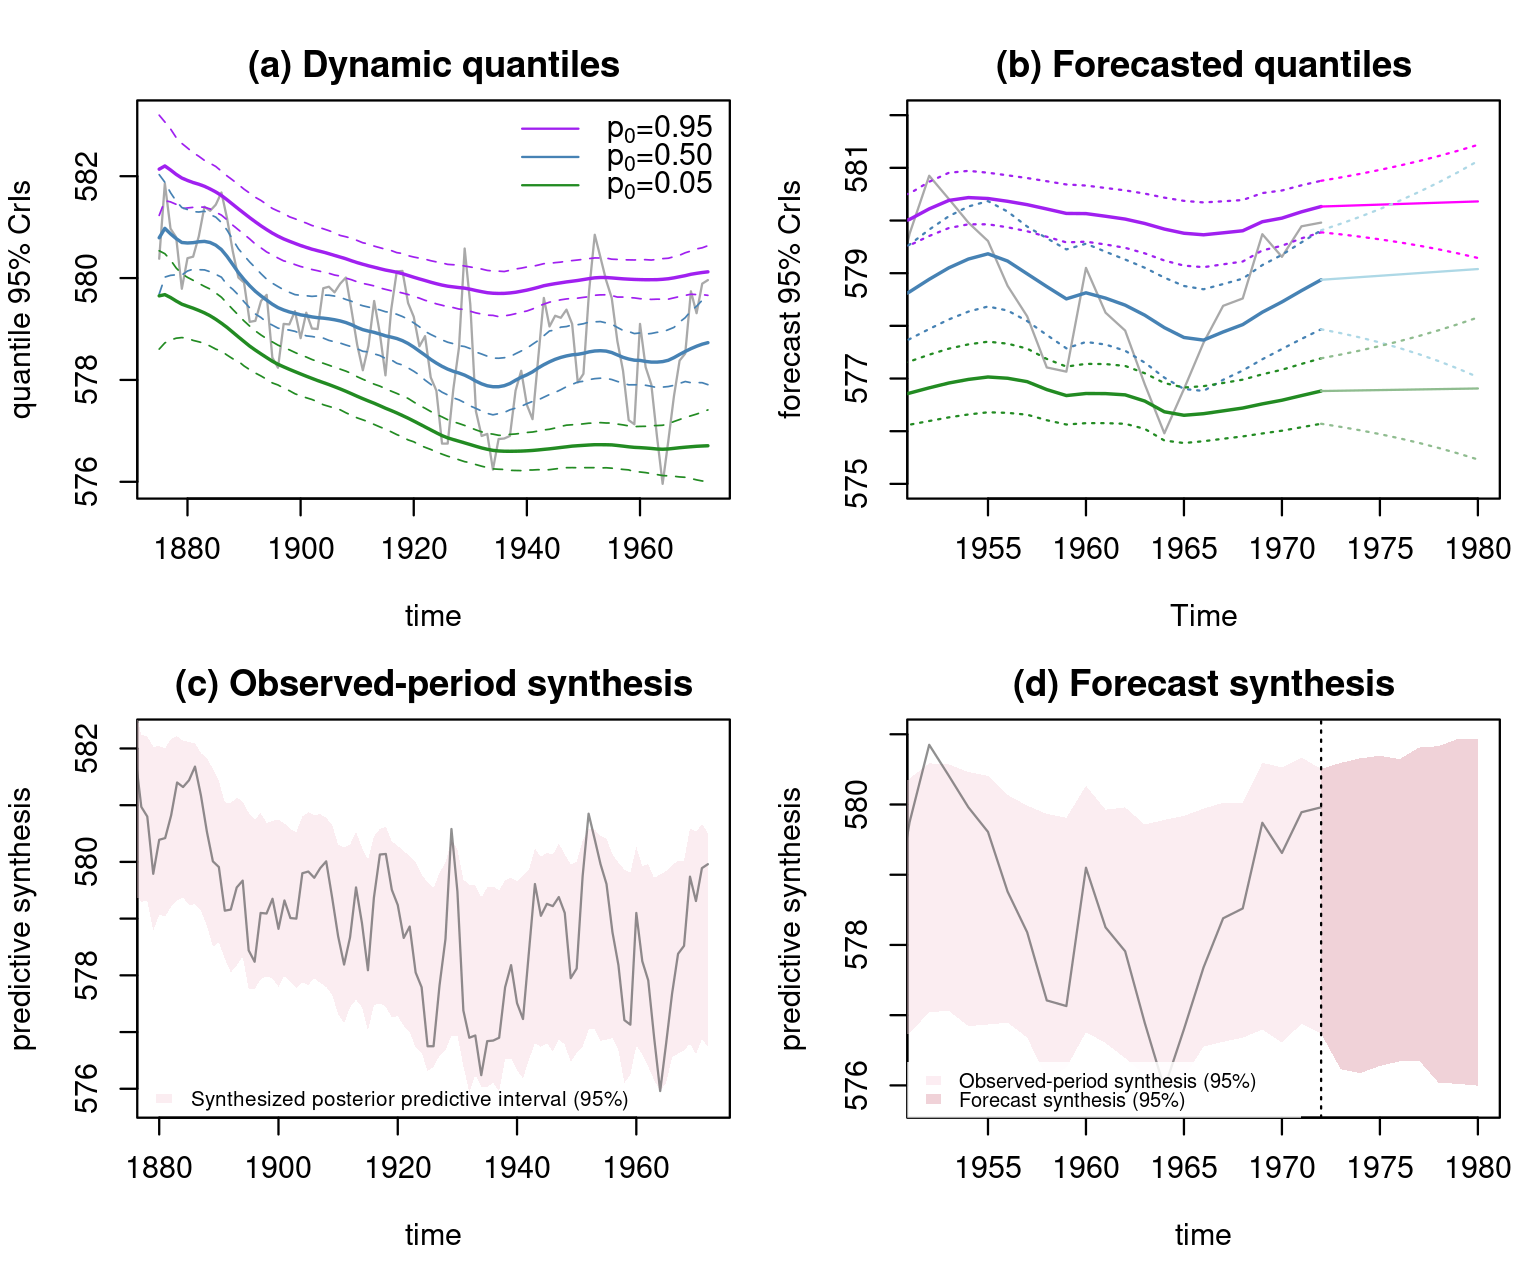
\includegraphics[width=0.9\textwidth]{figures/ch02-exdqlm/ex1quants.png}
\caption{Example 1: Lake Huron. Top-left: posterior mean estimates and 95\% CrIs of the estimated quantiles, plotted with the data (grey). Top-right: forecasted quantile estimates and 95\% credible intervals (seen after 1972), along with the filtered quantile estimates and 95\% credible intervals (seen from 1952 to 1972). Bottom-left: synthesized posterior predictive 95\% interval over the observed period. Bottom-right: observed-period synthesis near the forecast origin (lighter band) and synthesized posterior predictive 95\% interval over the eight-step forecast window (slightly darker rose band); the vertical dotted line marks the forecast origin.}
\label{exd:fig:ex1quants}
\end{figure}

Next, we forecast the $k=8$ step-ahead distributions starting in 1972. To do this, we first create the observational vector (\code{fFF}) and evolution matrix (\code{fGG}) that will be used in the forecast updates. In this case both are non-time-varying and identical to those used to estimate the quantile.


We plot the time series data in a narrower range for closer examination. Forecast objects can be created with \code{predict()} on a fitted dynamic model.
Here we create the forecast objects first and then call \code{plot()} with \code{add = TRUE}. Notice we start the forecast at the last time index of the data, i.e. \code{start.t = length(LakeHuron)}.



This generates a plot of the data with the forecasted quantile estimates and 95\% credible intervals (seen after 1972), along with the filtered quantile estimates and 95\% credible intervals (before 1972), for reference. Results can be seen in the top-right panel of Figure \ref{exd:fig:ex1quants}. The percentage in the CrIs can be modified with the parameter \code{cr.percent}.

When several quantile models are fitted separately, the package also allows their posterior predictive draws to be combined into a single coherent predictive distribution through \code{quantileSynthesis()}. Each fitted model contributes local predictive information near its target quantile, and the synthesis step interpolates across these quantile-specific draws to obtain one posterior predictive distribution. When independently fitted quantiles induce crossing, optional monotonicity corrections based on isotonic adjustment and monotone rearrangement are available \citep{exd-barlow1972,exd-chernozhukov2010}. The synthesis operates on posterior predictive draws indexed by quantile level, so the input fits need not use identical skewness restrictions. For the Lake Huron example, we combine exDQLM tail fits at \(p_0=0.05\) and \(0.95\) with the fixed-\(\gamma\) DQLM median fit \code{M50.dqlm}.



The recorded run uses the package's default isotonic adjustment and monotone rearrangement. The stored synthesized quantile summaries have no remaining crossings over the observed period.

Because the argument \code{return.draws = TRUE} was used, each object stores posterior predictive forecast draws in the return value \code{samp.fore}. This allows us to apply the same synthesis step to the eight-step forecast horizon.



The same correction settings are used for the forecast synthesis, and the eight-step synthesized forecast summaries are also ordered across the three input quantile levels.

The objects \code{syn.obs} and \code{syn.fore} have class \code{exdqlmSynthesis}, so the corresponding \code{plot()} method displays the synthesized posterior predictive intervals. The first synthesis panel in Figure~\ref{exd:fig:ex1quants} shows the observed-period interval. The second uses the same synthesis near the forecast origin, overlays the forecast synthesis, and shades the one-step bridge from the final observed interval to the first forecast interval.



%%%%%%%%%%%%%%%%%%%%%%%%%%%%%%%%%%%%%%%%%
%%%%%%%%%%%%%%%%%%%%%%%%%%%%%%%%%%%%%%%%%
%%%%%%%%%%%%%%%%%%%%%%%%%%%%%%%%%%%%%%%%%

\subsection{Sunspots}
\label{exd:sec:ex2}

The second example uses the yearly Sunspot time series from the package \pkg{datasets}.



The data are yearly counts for sunspots from 1700 to 1988, shown in Figure \ref{exd:fig:ex2quant}. In this example we show how to use the \pkg{dlm} package to create the state-space model, combine blocks of a state-space model, apply the LDVB approximation through \code{exdqlmLDVB()}, perform visual model diagnostics to compare the exDQLM with the DQLM, and use those diagnostics for discount-factor selection.

Upper-tail sunspot activity is a natural setting for illustrating dynamic quantile modeling of cyclic count data. We therefore model the \(0.85\) quantile in this example. Although sunspot activity is recorded as a count, we use the continuous exAL working likelihood to model its upper conditional quantile; the example is not intended as a discrete-count likelihood analysis. Again, we begin by building the state-space structure used to estimate the quantile. Here we choose to model the quantile with a first order polynomial trend component as well as a Fourier form seasonal component that incorporates a fundamental period every 11 observations (years), as well as some of its corresponding harmonics. This results in a dynamic model with a total of 9 state parameters, 1 for the first order polynomial component and 8 for the seasonal component. The \pkg{exdqlm} functions are compatible with time-invariant \code{dlm} objects from the \pkg{dlm} package. For example, we create the first order trend component with the function \code{dlmModPoly()} from the \pkg{dlm} package, then use \code{as.exdqlm()} to turn the output into an \code{exdqlm} object.

The initial level prior is centered at 50 sunspots, a rounded count-scale value chosen before fitting, with prior standard deviation 50 to keep the level weakly informative on the observed count scale. Next, we construct the seasonal component with our \code{seasMod()} function. Sunspot cycles are commonly modeled with an approximately 11-year period; we include the first four Fourier harmonics in the component.

To combine the two components into a single state-space structure, we add the two \code{exdqlm} objects.

Adding the two model components produces a block-composed state-space model with one trend state and eight seasonal states.

We will apply discount factors by component, i.e. a discount factor of $0.9$ for the trend component of dimension $1$ and a discount factor of $0.85$ for the seasonal component of dimension $8$. This discounting strategy can be applied with arguments \code{df = c(0.9, 0.85)} and \code{dim.df = c(1, 8)}.

\begin{figure}[t]
\centering
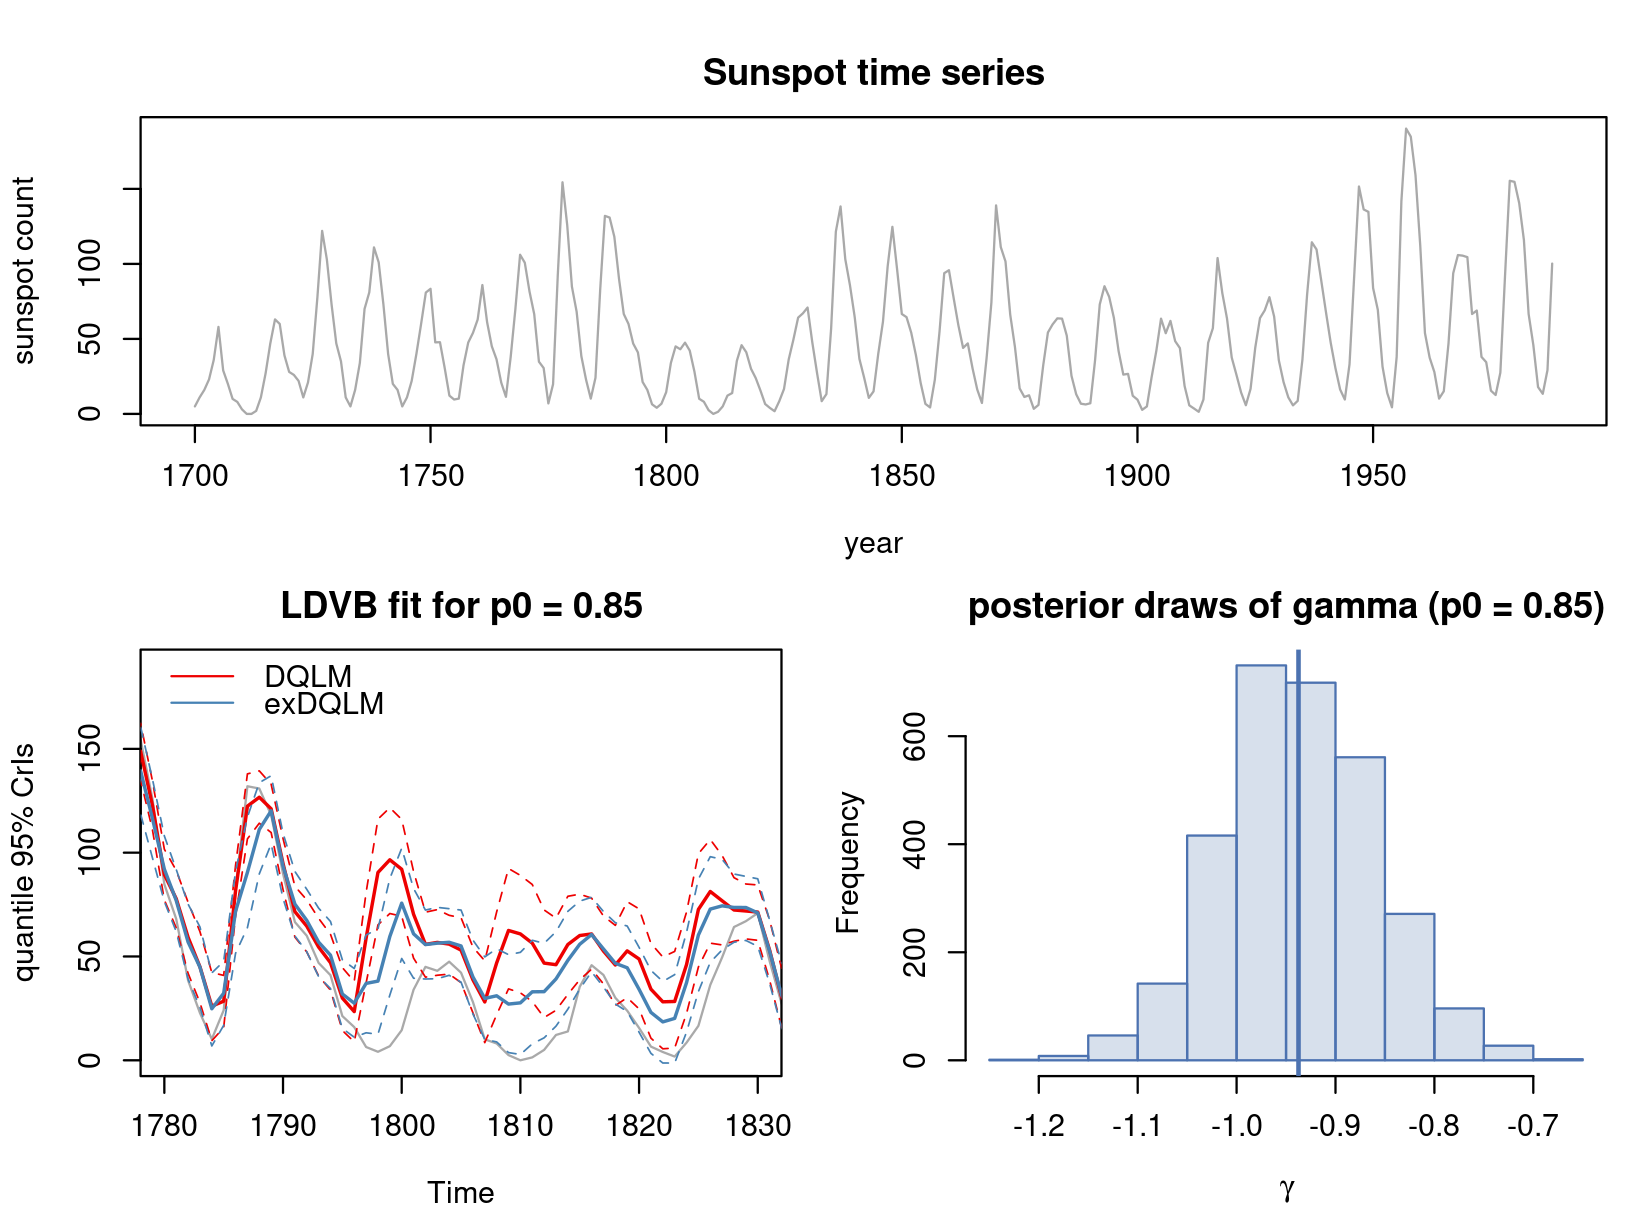
\includegraphics[width=1\textwidth]{figures/ch02-exdqlm/ex2quant.png}
\caption{Example 2: Sunspots. Top: The sunspot time series from 1700 to 1988. Bottom left: posterior mean estimates and 95\% CrIs of the estimated quantiles from the DQLM (red) and exDQLM (blue), plotted with the data (grey) from 1780 to 1830. Bottom right: Histogram of samples from the approximated posterior distribution of $\gamma$ under the exDQLM.}
\label{exd:fig:ex2quant}
\end{figure}

We call the function \code{exdqlmLDVB()} to obtain the LDVB approximations. We use the routine with argument \code{dqlm.ind = TRUE} to estimate the DQLM, as well as with the default settings to estimate the exDQLM. In this example we set \code{sig.init = 2} as the starting value for the LDVB scale update, use \code{n.samp = 3000}, and suppress iteration output with \code{verbose = FALSE}.



The fitted objects can be summarized with the \code{summary()} generic, which reports the model class, sample size, state dimension, discount factors, convergence iterations, and run time. For this dataset of length 289, the DQLM LDVB fit completes more quickly, while the corresponding exDQLM LDVB fit is more computationally demanding because the skewness parameter is estimated rather than fixed. The timing comparison in Table \ref{exd:tab:ex2bench} reports the values from the recorded benchmark setting. These runtimes are fit elapsed times stored in the returned fit objects; they are intended for within-setting comparison and should not be interpreted as machine-independent timing constants.

We can visualize the differences between the two resulting dynamic quantiles with the fitted-object \code{plot()} method, shown in the lower-left panel of Figure \ref{exd:fig:ex2quant}. For clarity we limit that panel to years 1780 to 1830.



\begin{figure}[t]
\centering
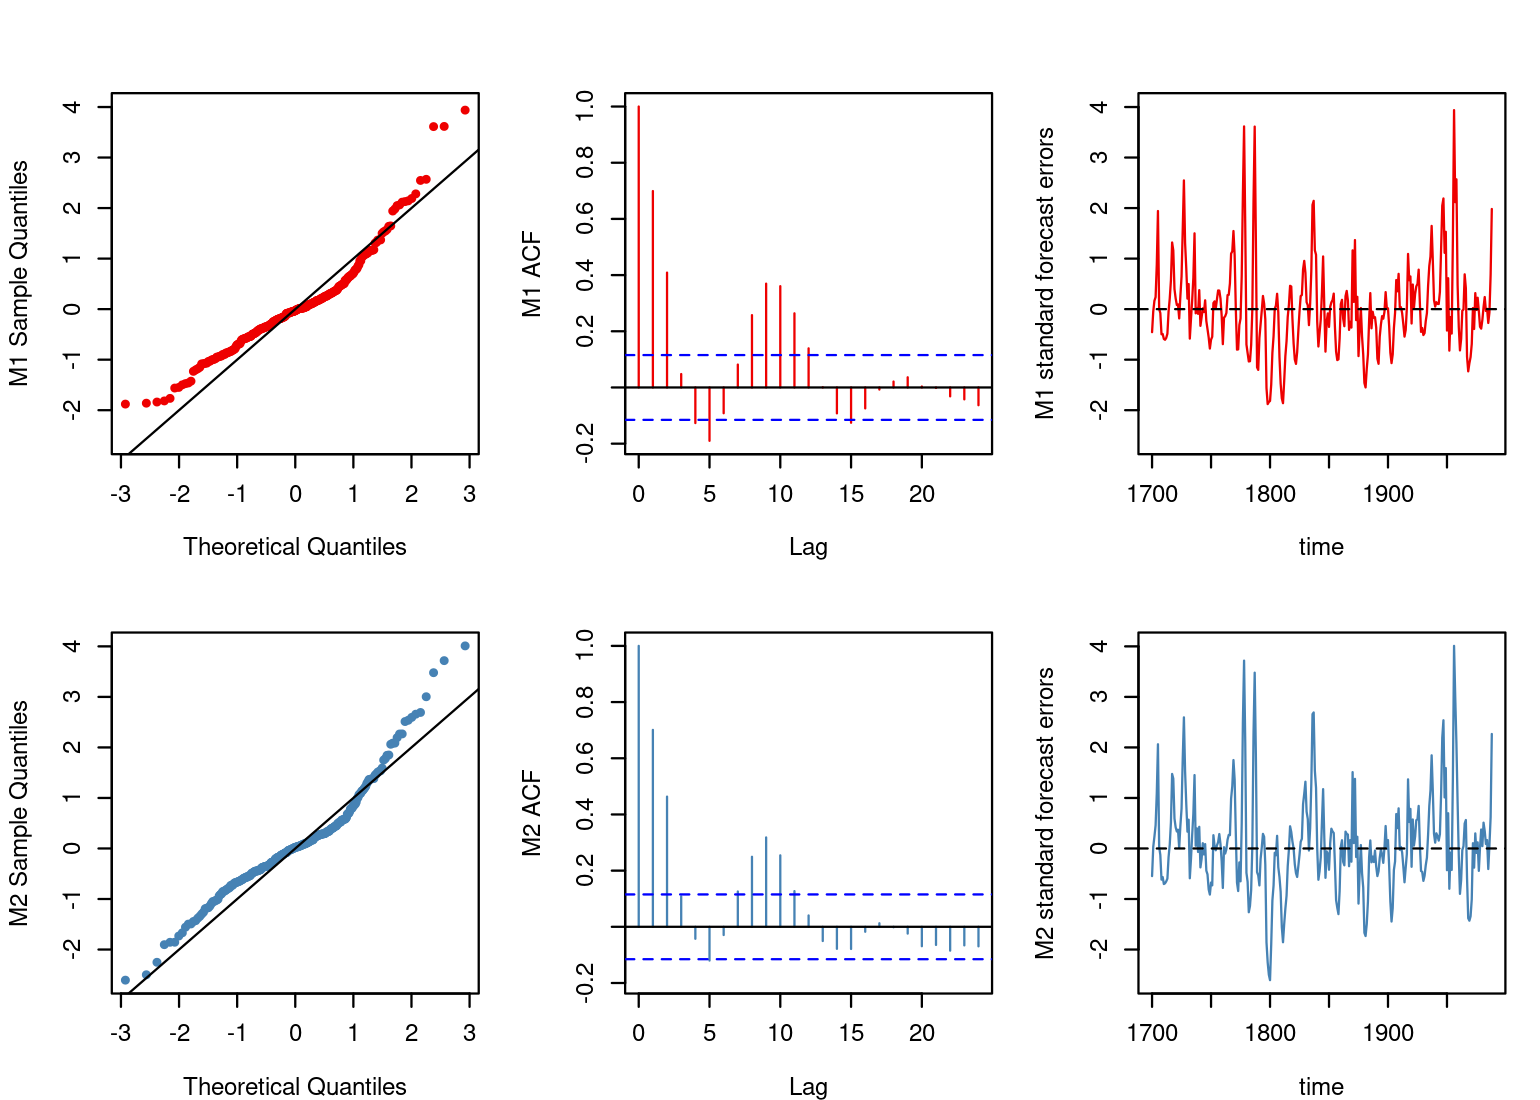
\includegraphics[width=1\textwidth]{figures/ch02-exdqlm/ex2checks.png}
\caption{Example 2: Sunspots. The QQ plots (left column), ACF plots of the PIT sequence (center column), and MAP one-step-ahead standardized forecast errors (right column) from the DQLM (red) and exDQLM (blue).}
\label{exd:fig:ex2checks}
\end{figure}

To examine whether the added flexibility of the exDQLM is supported by the fitted approximation, we can also visualize the approximate posterior distribution of the skewness parameter $\gamma$ by plotting the samples from the corresponding variational distribution, also seen in Figure \ref{exd:fig:ex2quant}. The approximate posterior mass lies away from zero, supporting the additional skewness flexibility for this upper-quantile fit.



To further examine the two models, we use the \code{diagnostics()} method to create an object of class \code{exdqlmDiagnostic} and then call its \code{plot()} method. The results are seen in Figure \ref{exd:fig:ex2checks}. These diagnostic plots are based on the MAP one-step-ahead standardized forecast errors produced by the filtering recursion, together with the corresponding probability integral transform (PIT) sequence. Thus the figure summarizes the fitted diagnostic sequence rather than posterior bands for residuals.



The \code{diagnostics()} method can also be used for a coarse in-sample comparison of candidate model specifications. Here we examine whether the discount factor used for the seasonal component is reasonable under the reported diagnostic criteria. We create a grid of possible discount factors, run the LDVB approximation for each candidate model, and compare the resulting CRPS and KL values. Because these criteria are computed using the observations employed to fit each model, this exercise is a diagnostic screening rather than an out-of-sample predictive validation. We use CRPS as the primary comparison criterion and KL divergence as a complementary calibration check; the selected discount-factor specification is the row with the smallest CRPS.


On this coarse grid, the CRPS and KL criteria agree and both select the seasonal discount factor \(0.85\), so the choice used above is retained.

To compare the fast variational approximation with posterior simulation, we fit matched DQLM and exDQLM specifications with \code{exdqlmMCMC()}. The MCMC fits use the same state-space model, quantile level, and discount factors as the LDVB fits, with 2000 burn-in iterations and 3000 retained draws.



\begin{table}[t!]
\centering
\TableStyle
\begin{tabular}{@{}llrrrr@{}}
 \toprule
 model & method & \shortstack{runtime\\(s)} & KL & CRPS & PPLC \\
 \midrule
 \tworowcell{DQLM} & LDVB & \textbf{22.53} & \textbf{0.133} & 8.525 & 3851.4 \\
 & MCMC & 125.48 & 0.170 & \textbf{7.580} & \textbf{2966.0} \\
 \midrule
 \tworowcell{exDQLM} & LDVB & \textbf{73.46} & \textbf{0.107} & 6.558 & 3015.2 \\
 & MCMC & 174.66 & 0.212 & \textbf{5.120} & \textbf{2206.8} \\
 \bottomrule
\end{tabular}
\caption{Example 2: representative dynamic benchmark for the DQLM and exDQLM fits at \(p_0 = 0.85\). Each row reports fit runtime together with the deterministic KL normality diagnostic, the mean CRPS from posterior predictive empirical quantiles, and the posterior predictive loss criterion (PPLC). The LDVB rows use \code{n.samp = 3000}. The MCMC rows use 2000 burn-in iterations and 3000 retained draws. Runtimes are fit elapsed times stored in the returned fit objects and exclude diagnostic calculations, plotting, table construction, and document rendering. They were measured under benchmark setting B on an Intel Xeon E5-4650 CPU with \proglang{R} 4.6.0, \pkg{exdqlm} version 1.1.2, the C++ MCMC implementation in \code{"fast"} mode, and \code{exdqlm.cpp\_threads = 1L}. Because the columns are the comparison metrics, bold entries indicate the smaller value within each model block; displayed ties are left unbolded.}
\label{exd:tab:ex2bench}
\end{table}

Table \ref{exd:tab:ex2bench} gives a compact runtime-and-diagnostic comparison. \code{print()} on the following data frame will produce the results.



Within each model class, LDVB is substantially faster. For both DQLM and exDQLM, LDVB gives the smaller KL value, while MCMC gives smaller CRPS and PPLC values. Comparing model classes within each inferential method, the exDQLM improves the LDVB diagnostics relative to the DQLM, and under MCMC it improves the predictive-score criteria CRPS and PPLC. The comparison shows why runtime is reported together with predictive criteria rather than by itself.

%%%%%%%%%%%%%%%%%%%%%%%%%%%%%%%%%%%%%%%%%
%%%%%%%%%%%%%%%%%%%%%%%%%%%%%%%%%%%%%%%%%
%%%%%%%%%%%%%%%%%%%%%%%%%%%%%%%%%%%%%%%%%

\subsection{Big Tree water flow}
\label{exd:sec:ex3}


For the third example, we use observed average monthly water flow (cubic feet
per second) at the Big Tree gauge of the San Lorenzo River in Santa Cruz
County, CA \citep{exd-btflow}. The \pkg{exdqlm} version 1.1.2 used for this
analysis includes these measurements as the monthly time series \code{BTflow},
which extends through March 2026. Here we use the complete overlap between
\code{BTflow} and the package data frame \code{climateIndices},
giving 432 monthly observations from January
1987 through December 2022. The final 18 months, July 2021 through December
2022, are not used for fitting and are shown later in a conditional forecast
display. This example illustrates the transfer-function workflow: building a
baseline dynamic quantile model, adding external covariates through the
transfer-function state augmentation, examining fitted components, and
forecasting conditionally on future covariate values.

\begin{figure}[t]
\centering
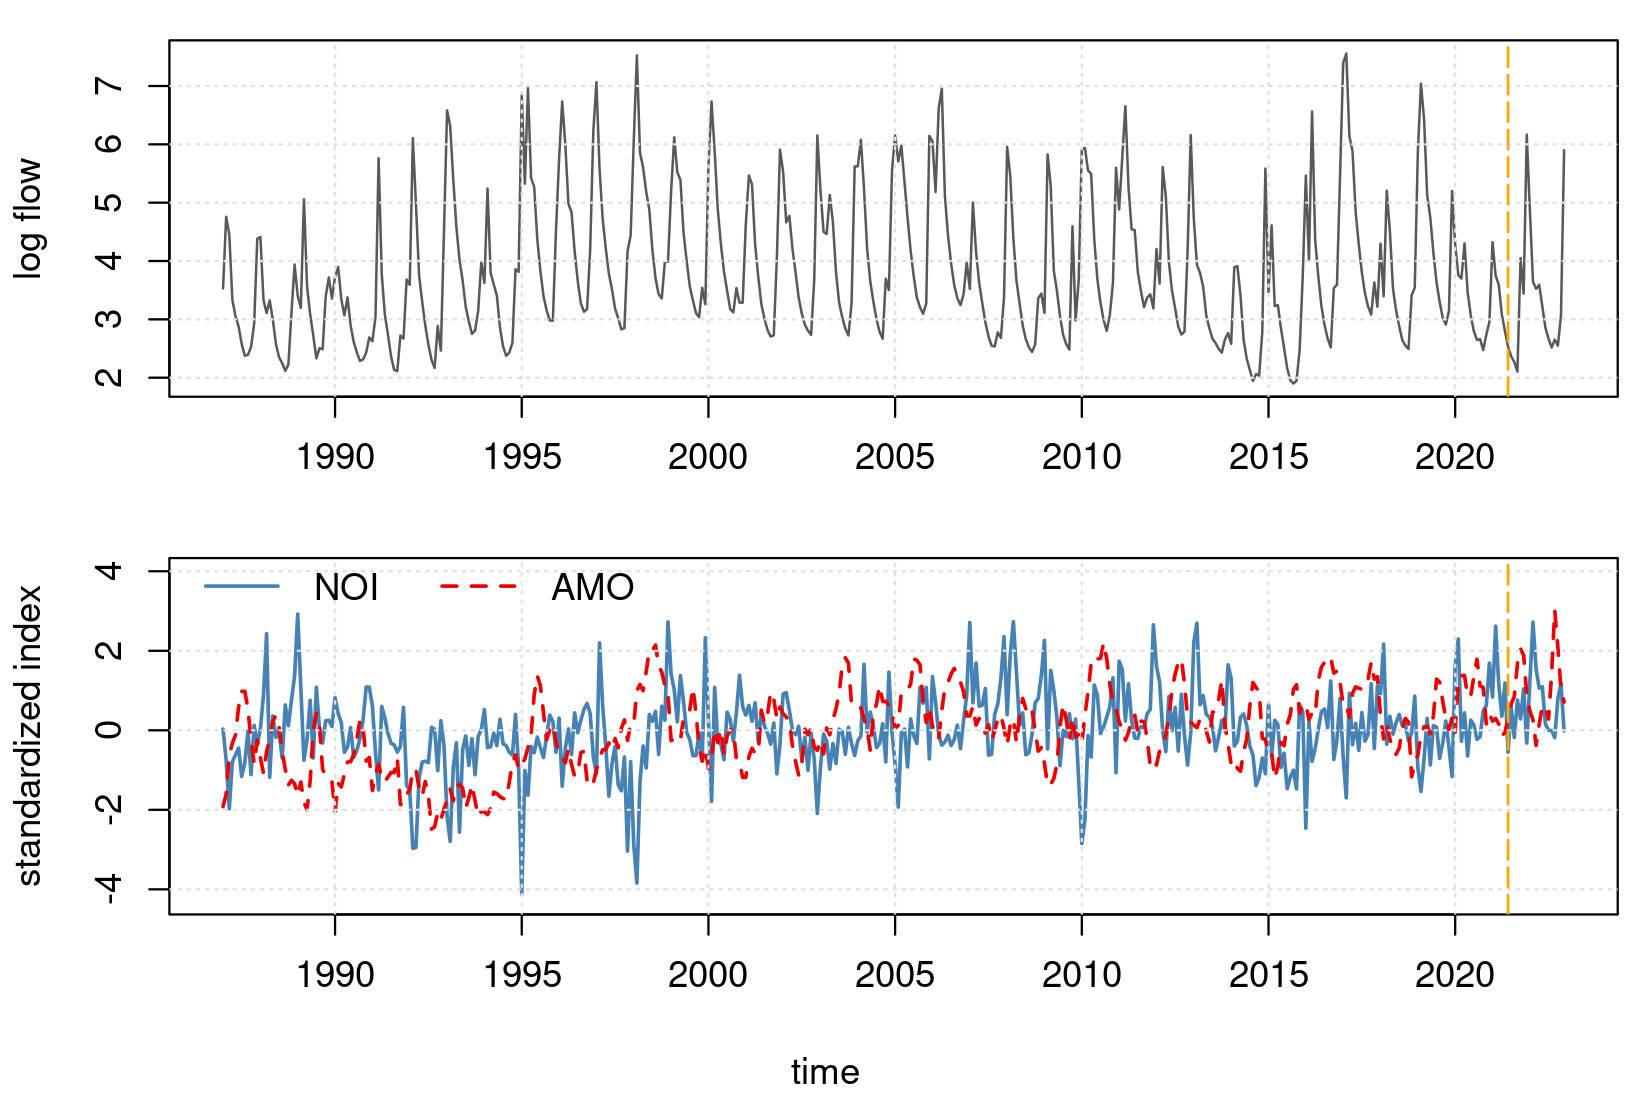
\includegraphics[width=1\textwidth]{figures/ch02-exdqlm/ex3data.png}
\caption{Example 3: Big Tree water flow. Top: observed average monthly water
flow at the Big Tree gauge of the San Lorenzo River in Santa Cruz County, CA,
plotted on the log scale. Bottom: standardized monthly values of the Northern
Oscillation Index (NOI) and Atlantic Multidecadal Oscillation (AMO) index. The
displayed modeling window spans January 1987 through December 2022, and the
vertical dashed line marks the beginning of the held-out forecast window in
July 2021.}
\label{exd:fig:ex3data}
\end{figure}

We focus on the lower-tail quantile \(p_0=0.15\), which represents lower
monthly-flow behavior on the log scale. As transfer-function inputs, we use two
monthly climate indices from \code{climateIndices}: the Northern Oscillation
Index (NOI) and the Atlantic Multidecadal Oscillation (AMO) index. These indices
come from the NOAA Physical Sciences Laboratory climate-index collection
\citep{exd-noaaClimateIndices} and provide a compact setting for illustrating
external-input effects. The covariates are standardized using the training
window only. In the forecast display, NOI and AMO values over the held-out
months are treated as known future inputs; the display is therefore conditional
on those covariates rather than an operational forecast of the climate indices.
The complete overlap used here has 432 monthly observations. The first 414
observations, January 1987 through June 2021, form the training period; the final
18 observations, July 2021 through December 2022, form the forecast holdout.
The external replication script records the date construction, merge,
training-window split, and training-window scaling used for this example.



Figure~\ref{exd:fig:ex3data} shows the aligned response and covariate series.



The baseline state-space model contains a first-order polynomial trend and a Fourier-form seasonal component with period 12. The seasonal block includes \(h = 1\), \(h = 2\), and \(h \approx 0.147\), corresponding to annual, semiannual, and approximately 7-year cycles on the monthly scale.
The low-frequency harmonic \(h=0.1469118636\) follows the specification developed in \citet{exd-me}; see that work for its motivation and selection.

The initial log-flow level prior is centered at \(\log(50)\), corresponding to
a fixed 50 cubic feet per second reference value, with prior standard deviation
1 on the log scale. This gives a broad domain-scale prior without using the
training response to center the state prior. The standardized climate coefficients are assigned zero-centered normal priors
with variance 1. On the log-flow scale this is intentionally weakly informative:
it allows either climate index to shift the lower-tail quantile materially while
still regularizing the example around no climate effect.

We compare three models built from the same trend and seasonal baseline. The
first, \code{M0}, contains no climate covariates. The second, \code{MREG}, adds
NOI and AMO as direct contemporaneous regressors using \code{regMod()}. The
third, \code{MTF}, adds the same two covariates through the transfer-function
structure from Section \ref{exd:sec:tf}. For all three models, the trend and
seasonal discount factors are set to 0.99. To keep the climate-effect
comparison simple, the direct-regression coefficients in \code{MREG} and the
instantaneous transfer coefficients \(\psi_t\) in \code{MTF} use discount
factor 1, so these coefficient states are static over time. The transfer
accumulated-effect state \(\zeta_t\) retains discount factor 0.99.

The transfer rate \(\lambda\) is selected using the training period only. Guided
by an initial coarse scan, the replication script fits the transfer model over
\(\lambda\in\{0.70,0.75,0.80,0.85,0.90,0.95,0.99\}\) and chooses the value with
the smallest posterior predictive loss criterion (PPLC) from
\code{diagnostics()}. The held-out months are not used in this selection
step. The option \code{exdqlm.max\_iter} sets the LDVB iteration cap used in
the recorded run; the exact selection loop and convergence controls remain in
the external replication script.



The final models are fit on January 1987 through June 2021. We use the LDVB implementation for all three models; the corresponding MCMC implementation is available when posterior simulation is desired.

\begin{figure}[!t]
\centering
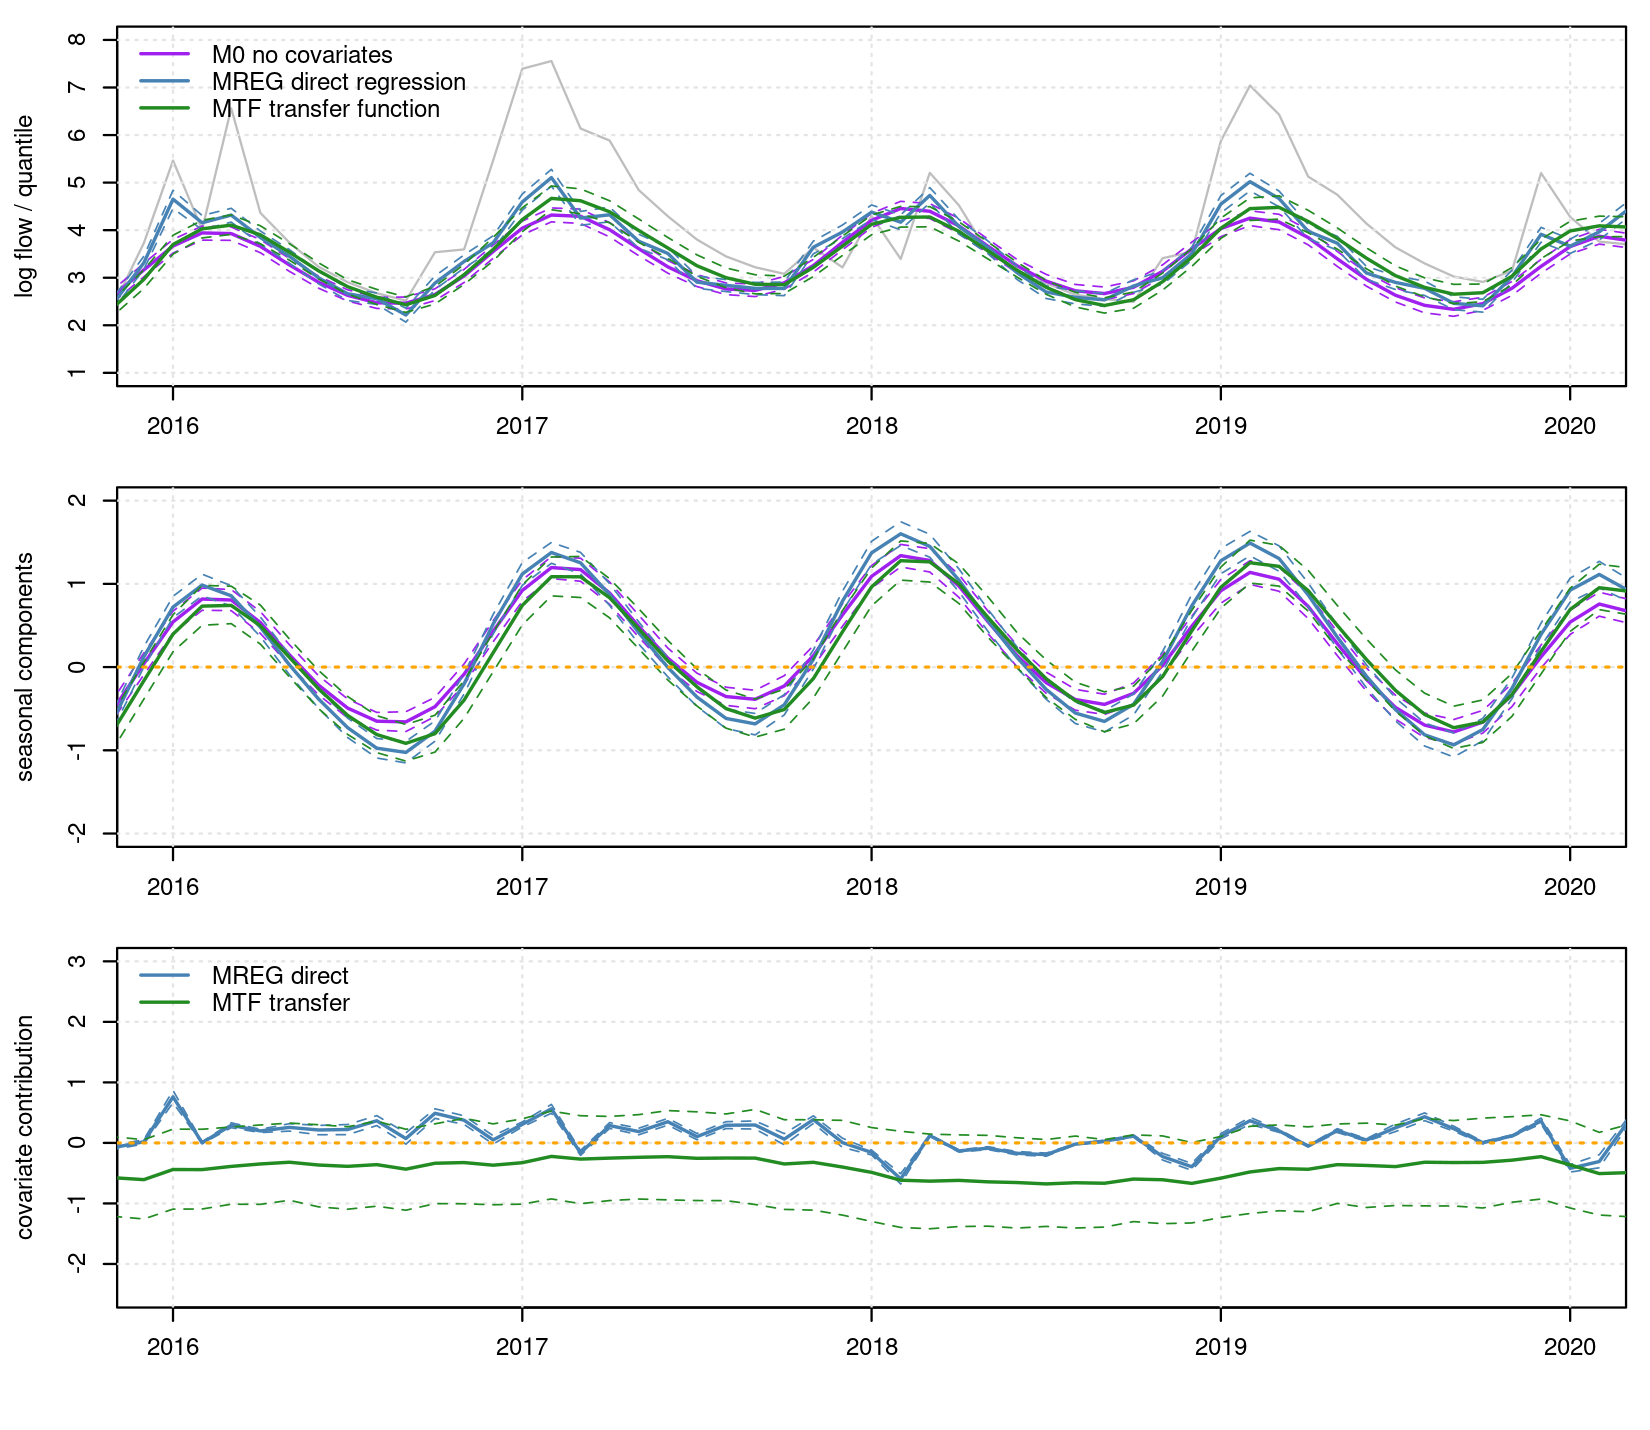
\includegraphics[width=0.92\textwidth]{figures/ch02-exdqlm/ex3quantcomps.png}
\caption{Example 3: Big Tree water flow. Top: posterior mean estimates and 95\% CrIs of the fitted \(0.15\) quantile from the no-covariate baseline \code{M0} (purple), direct-regression model \code{MREG} (blue), and transfer-function model \code{MTF} (green), plotted with the data (grey) from 2016 to 2020. Middle: posterior mean estimates and 95\% CrIs of the combined seasonal components implied by the annual, semiannual, and low-frequency harmonics. Bottom: posterior mean estimates and 95\% CrIs of the direct-regression contribution in \code{MREG} and the transfer-function contribution in \code{MTF}. The horizontal orange dotted lines are at zero for reference.}
\label{exd:fig:ex3quant}
\end{figure}



The upper panel of Figure \ref{exd:fig:ex3quant} compares the fitted \(0.15\)
quantiles from the three training fits over 2016--2020. We first plot the data, then call \code{plot()} with \code{add = TRUE} on the three fitted objects to draw the model fits on common axes.



The fitted lower-tail quantile paths are similar because the trend and seasonal components explain
much of the broad annual structure. The component panels of Figure \ref{exd:fig:ex3quant} clarify the model
differences: the middle panel shows that the seasonal contribution is similar
across models, while the lower panel separates the contemporaneous climate-index
contribution in \code{MREG} from the accumulated transfer contribution in
\code{MTF}. Component and state views are available from the fitted-object
\code{plot()} method by specifying the parameter \code{type = "component"} or \code{type = "state"}, respectively. We
begin with the combined seasonal contribution. Because the seasonal block
contains three harmonics, this contribution is formed from the second through
seventh elements of the state vector. The middle panel of Figure
\ref{exd:fig:ex3quant} shows the resulting seasonal estimates for the three models
over the same 2016--2020 window.


The lower panel of Figure \ref{exd:fig:ex3quant} displays the climate-index
contributions induced by the standardized NOI and AMO covariates. For
\code{MREG}, indices 8 and 9 are the direct-regression coefficient states. For
\code{MTF}, index 8 is the accumulated transfer effect \(\zeta_t\). This
separates contemporaneous and lagged climate-index components from the common
trend and seasonal baseline, even when the fitted quantiles themselves are
visually close.



The augmented-state summaries provide the corresponding parameter-level
diagnostic. As described in Section \ref{exd:sec:tf}, \(\zeta_t\) controls the
accumulated transfer effect and the \(\psi_t\) states determine how the
contemporaneous covariates enter that transfer term. In this example the
\(\psi_t\) discount factors are set to 1, so the bottom panels summarize static
NOI and AMO coefficients within the transfer-function model. The stored
summaries show the NOI coefficient below zero, whereas the AMO coefficient is
close to zero and its pointwise 95\% CrI overlaps zero. Setting
\code{type = "state"} in \code{plot()} plots a single element of the
augmented state vector \(\tilde{\vect{\theta}}_t\). In this fitted model,
indices 8, 9, and 10 correspond to \(\zeta_t\), \(\psi_{\mathrm{NOI},t}\), and
\(\psi_{\mathrm{AMO},t}\), respectively. We therefore use this analysis to
illustrate the specification,
inspection, and forecasting of lagged transfer effects, rather than to claim that
both climate indices have separately resolved transfer coefficients in these
data.



The fitted object also reports \code{median.kt}, the median number of time steps
until the transfer effect on the \(0.15\) quantile is less than or equal to
\(1\mathrm{e}{-3}\), as discussed in Section \ref{exd:sec:tf}. Here
\code{median.kt} is approximately 350.20, reflecting the highly persistent
transfer effect implied by the selected \(\lambda\) at the upper end of the
candidate grid.


We next produce 18-month-ahead forecasts over the held-out window. The
future state-space matrices are passed through the \code{fFF} and \code{fGG}
arguments of the \code{predict()} method for fitted dynamic objects. This
method returns \code{exdqlmForecast} objects. The external replication script
records the matrix construction, dimension checks, forecast calls, and output
handling. For \code{M0}, the future state-space matrices repeat the trend and
seasonal model.



For \code{MREG}, the future observation matrix includes the held-out NOI and AMO values as direct regressors.



For \code{MTF}, the future matrices include the held-out NOI and AMO values through the transfer-function augmentation.



Finally, Figure \ref{exd:fig:ex3forecast} overlays the filtered estimates before the forecast
origin and the conditional forecasts after it.



The numerical comparison in Table
\ref{exd:tab:ex3} uses \code{diagnostics()} so that all reported quantities
are exported package diagnostics, as defined in Section \ref{exd:sec:diags}. These
diagnostics are computed from the final-training fitted objects.



\begin{table}[ht!]
\centering
\TableStyle
\begin{tabular}{@{}lrrr@{}}
 \toprule
 Model & KL & CRPS & PPLC \\
 \midrule
 \code{M0} no covariates & 0.122 & 0.416 & 177.9 \\
 \code{MREG} direct regression & \textbf{0.108} & 0.347 & 160.6 \\
 \code{MTF} transfer function & 0.149 & \textbf{0.314} & \textbf{141.7} \\
 \bottomrule
\end{tabular}
\caption[Big Tree water-flow diagnostics]{Example 3: Big Tree water flow. Package diagnostics from
\code{diagnostics()} for the no-covariate baseline \code{M0}, direct-regression model \code{MREG}, and transfer-function model \code{MTF}, computed on the final-training fitted objects. KL denotes the deterministic Kullback--Leibler normality diagnostic for the MAP standardized forecast errors, CRPS denotes the continuous ranked probability score, and PPLC denotes the posterior predictive loss criterion. Lower values are preferred; bold entries mark the smallest value for each diagnostic.}
\label{exd:tab:ex3}
\end{table}

Alternatively, Table
\ref{exd:tab:ex3forecastmetrics} reports held-out forecast scores over the final 18
months. These diagnostics are computed from the forecast objects using the corresponding \code{diagnostics()} method. The held-out observations are a required input for this method.



Table \ref{exd:tab:ex3} gives a mixed in-sample diagnostic comparison. The direct-regression model has the smallest KL value, while the transfer-function model has the smallest CRPS and PPLC values after selecting \(\lambda\) by training-period PPLC. The example shows how \pkg{exdqlm} supports three related dynamic quantile workflows: no external inputs, direct regression through \code{regMod()}, and lagged external-input effects through transfer functions.

\begin{table}[ht!]
\centering
\TableStyle
\begin{tabular}{@{}lrr@{}}
 \toprule
 Model & Check loss & CRPS \\
 \midrule
 \code{M0} no covariates & 0.120 & 0.473 \\
 \code{MREG} direct regression & \textbf{0.114} & \textbf{0.399} \\
 \code{MTF} transfer function & 0.221 & 0.803 \\
 \bottomrule
\end{tabular}
\caption{Example 3: Big Tree water flow. Held-out forecast metrics over July 2021 through December 2022, computed with \code{diagnostics()} from \code{exdqlmForecast} objects returned by \code{predict(..., return.draws = TRUE)}. Check loss is computed at \(p_0=0.15\), and CRPS is computed from posterior predictive forecast draws using the integrated-quantile-score approximation. Lower values are preferred; bold entries mark the smallest value in each column.}
\label{exd:tab:ex3forecastmetrics}
\end{table}

In the held-out comparison, \code{MREG} has the smallest check loss and CRPS, followed by the no-covariate model \code{M0}; \code{MTF} has the largest value for both metrics. Thus, selecting the transfer parameter \(\lambda\) using training-period PPLC does not make the transfer-function specification the best held-out forecasting model in this example. The purpose of \code{MTF} here is to demonstrate how persistent lagged covariate effects can be specified, inspected, and forecast using the package, rather than to claim predictive superiority over direct regression for these data.

\begin{figure}[!htb]
\centering
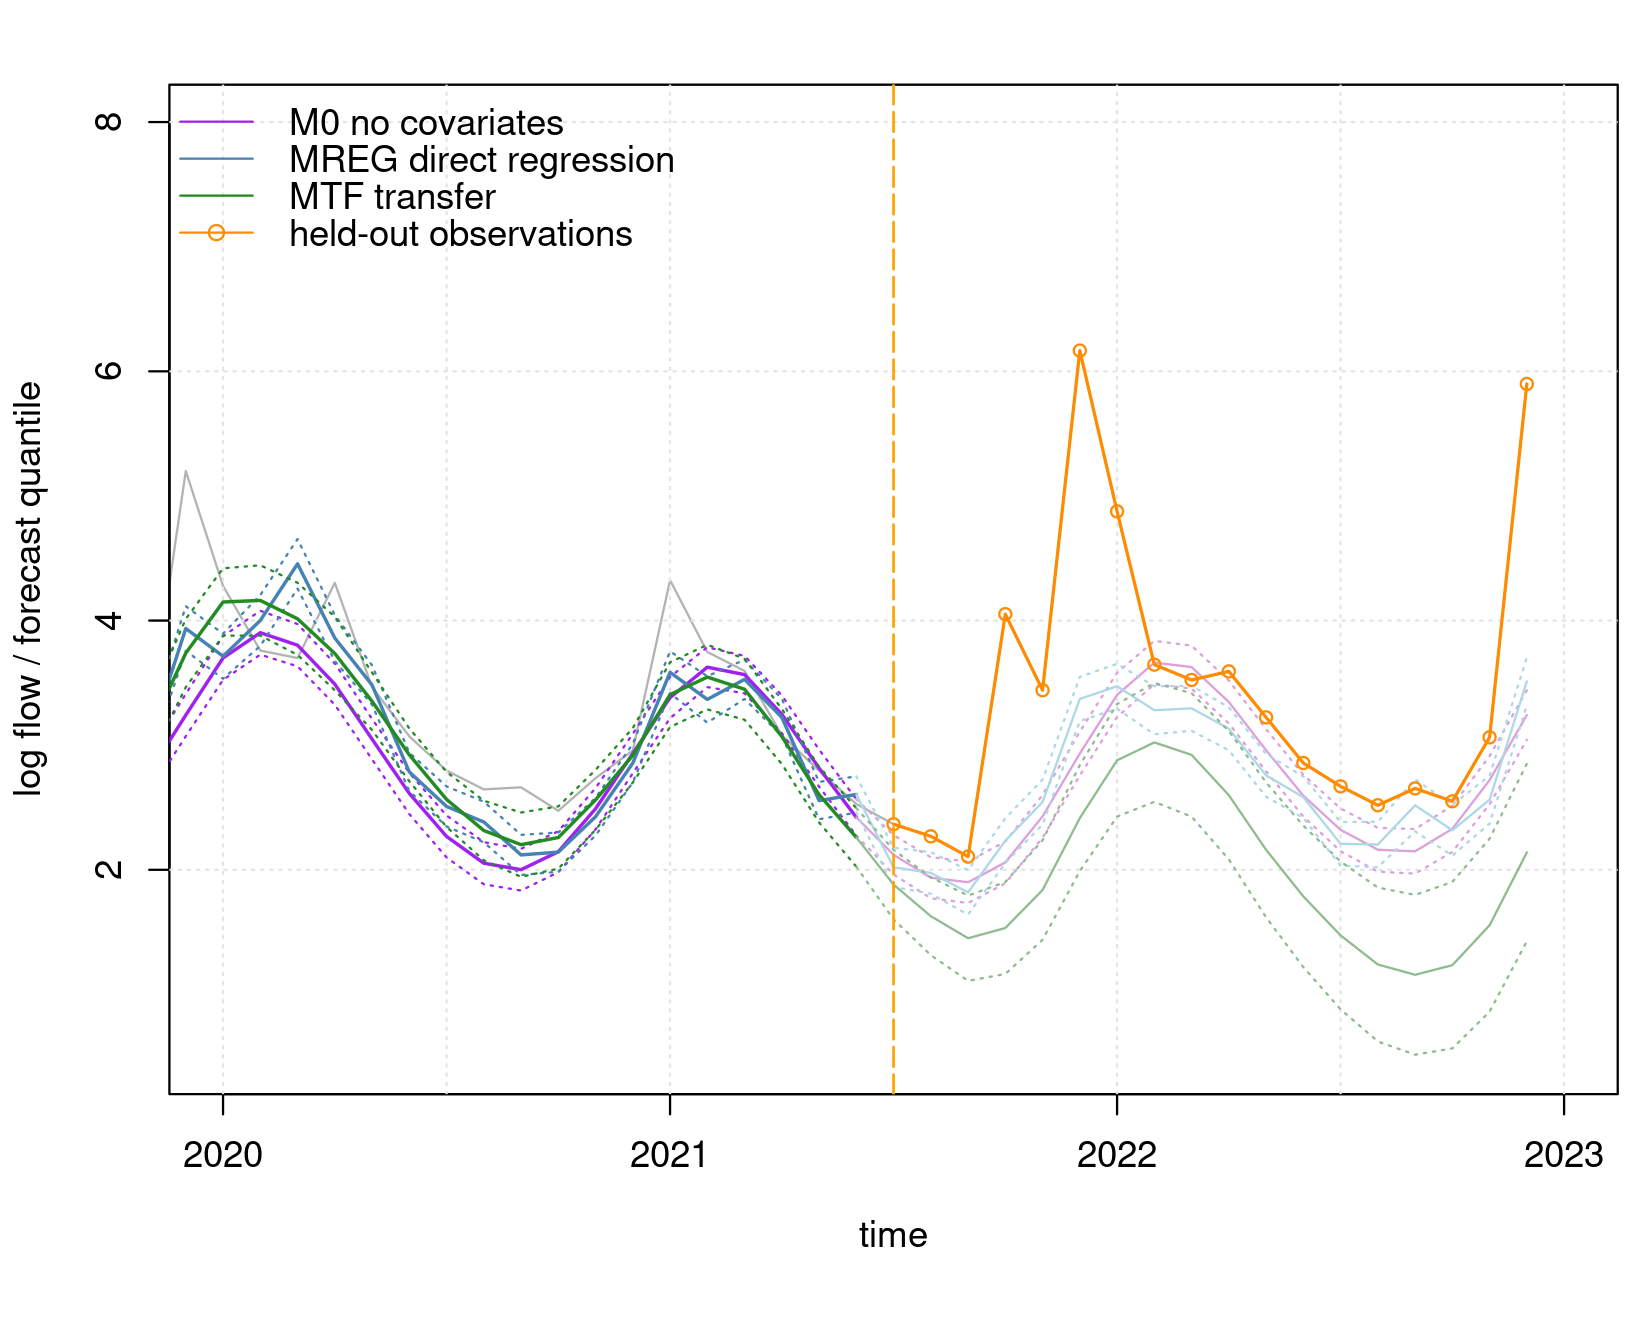
\includegraphics[width=0.82\textwidth]{figures/ch02-exdqlm/ex3forecast.png}
\caption{Example 3: Big Tree water flow. Held-out 18-month conditional forecast
display from July 2021 through December 2022. The vertical dot-dashed line marks
the forecast origin after the final training month, June 2021. Solid lines
indicate posterior mean forecast quantiles and dotted lines indicate pointwise
95\% CrIs for \code{M0}, \code{MREG}, and \code{MTF}. Held-out observations are shown as orange circles. The forecasts are conditional on the observed holdout-period NOI and AMO values.}
\label{exd:fig:ex3forecast}
\end{figure}

%%%%%%%%%%%%%%%%%%%%%%%%%%%%%%%%%%%%%%%%%
%%%%%%%%%%%%%%%%%%%%%%%%%%%%%%%%%%%%%%%%%
%%%%%%%%%%%%%%%%%%%%%%%%%%%%%%%%%%%%%%%%%

\subsection{Static exAL regression on a simulated sparse Gaussian benchmark}
\label{exd:sec:ex4static}


To illustrate the static routines under sparse shrinkage, we consider a correlated Gaussian regression benchmark for which the target conditional quantile is known exactly. Let
\[
\mat{x}_i \sim \N_8(\mat{0}, \Sigma_x),\qquad (\Sigma_x)_{jk} = 0.5^{|j-k|},
\]
with sparse signal
\[
\vect{\beta}^\star = (3,\,1.5,\,0,\,0,\,2,\,0,\,0,\,0)^\top.
\]
We use the following benchmark data-generating mechanism.
For each target quantile level \(p_0\), we generate
\[
Y_i^{(p_0)} = \mat{x}_i^\top \vect{\beta}^\star + \sigma_\varepsilon \{Z_i - \Phi^{-1}(p_0)\},
\qquad Z_i \sim \N(0,1),\qquad \sigma_\varepsilon = 1.5.
\]
Then
\[
Q_Y(p_0 \mid \mat{x}_i) = \mat{x}_i^\top \vect{\beta}^\star,
\]
so the true \(p_0\)-quantile is the same sparse linear signal at each fitted quantile level. Note that this is a quantile-specific calibration benchmark: each target level is generated so that the known target quantile is the same sparse linear signal, rather than a single-response multi-quantile analysis. The Gaussian data-generating distribution does not coincide with the exAL working likelihood; the benchmark therefore evaluates recovery of a correctly specified conditional quantile under likelihood misspecification. Gaussian design matrices are generated with \code{MASS::mvrnorm()} from \pkg{MASS} \citep{exd-MASS}.
We use \(n = 160\) training observations and an independent holdout sample of size \(800\).



We fit separate static exAL models at \(p_0 \in \{0.05,0.25,0.50\}\). All fits use the Nishimura--Suchard regularized horseshoe prior \citep{exd-nishimura2023shrunken}, implemented in the package through \code{beta_prior = "rhs\_ns"}, with \(\tau_0 = 0.15\), fixed slab \(\zeta^2 = 9\), and an unshrunk intercept. We fit an LDVB approximation with \code{exalStaticLDVB()} using \code{n.samp = 3000}, and an MCMC fit with \code{exalStaticMCMC()} using \code{n.burn = 2000} and \code{n.mcmc = 3000}; the MCMC routine uses its default \code{collapsed\_slice} scale--skewness kernel and is warm-started from the LDVB fit. The lower-tail LDVB fit at \(p_0 = 0.05\) converges more slowly, so we allow a larger LDVB iteration budget there. Setting \code{al.ind = TRUE} (or equivalently \code{dqlm.ind = TRUE}) would recover the AL special case discussed in Section \ref{exd:sec:exdqlm}, but here we focus on the general static exAL model under sparse \code{rhs\_ns} shrinkage.



For static fits, the \code{diagnostics()} method summarizes fitted quantiles on a common design matrix and, when holdout responses or a reference quantile are supplied, reports predictive evaluation metrics such as check loss and reference-quantile error. It also stores posterior coefficient summaries that can be plotted with \code{plot(..., type = "coefficients")}. In this simulated example, the true coefficient vector is known, so Figure \ref{exd:fig:ex4static} overlays it as a visual reference. This truth overlay is optional through the parameter \code{beta.ref} and is not needed for real data applications.



\begin{figure}[!t]
\centering
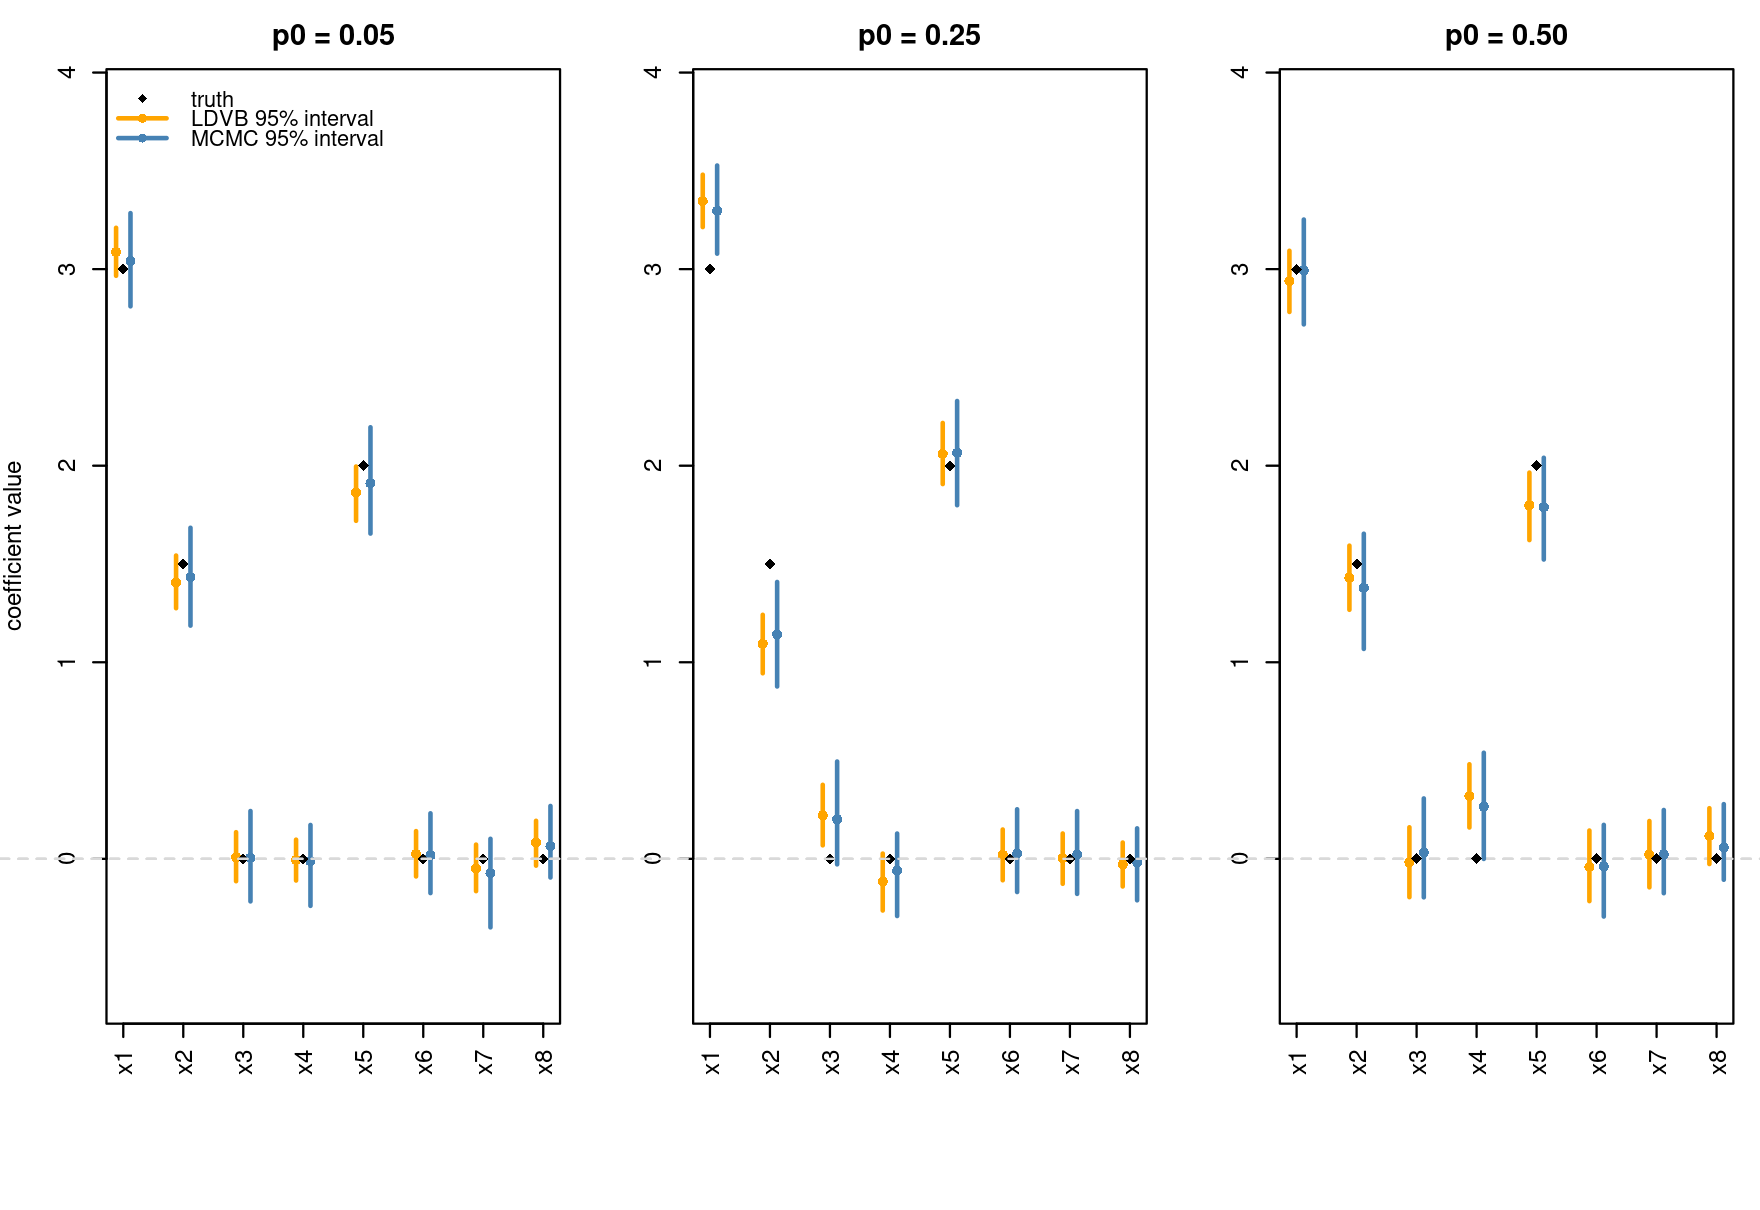
\includegraphics[width=0.95\textwidth]{figures/ch02-exdqlm/ex4static.png}
\caption{Example 4: sparse static exAL regression under the correlated Gaussian benchmark with the \code{rhs\_ns} prior. Black diamonds denote the true non-intercept coefficients, orange intervals denote LDVB 95\% posterior intervals, and blue intervals denote MCMC 95\% posterior intervals. Panels correspond to \(p_0 = 0.05, 0.25,\) and \(0.50\).}
\label{exd:fig:ex4static}
\end{figure}

Figure \ref{exd:fig:ex4static} shows that, in this simulated realization, both methods recover the main sparse signal structure and shrink most null coefficients toward zero across the lower tail, lower-middle quantile, and median. Recovery is not uniform across coefficients: the smaller active coefficient is more difficult in the median fit, and a few null-coefficient intervals can miss zero. Across the three panels, the MCMC intervals give cleaner active-signal recovery in the two lower-tail fits, while the median fit is closer; the LDVB intervals provide a faster approximation to the same coefficient-level summaries.

\begin{table}[t!]
\centering
\TableStyle
{\setlength{\tabcolsep}{3pt}
\begin{tabular}{@{}llrrrr@{}}
 \toprule
 \(p_0\) & method & \shortstack{runtime\\(s)} & \shortstack{active\\RMSE} & \shortstack{null\\MAE} & \shortstack{holdout\\qRMSE} \\
 \midrule
 \tworowcell{0.05} & LDVB & \textbf{31.46} & 0.108 & \textbf{0.034} & 0.673 \\
 & MCMC & 71.92 & \textbf{0.069} & 0.035 & \textbf{0.594} \\
 \midrule
 \tworowcell{0.25} & LDVB & \textbf{27.74} & 0.310 & 0.078 & 0.371 \\
 & MCMC & 71.19 & \textbf{0.271} & \textbf{0.065} & \textbf{0.329} \\
 \midrule
\tworowcell{0.50} & LDVB & \textbf{12.66} & \textbf{0.128} & 0.103 & 0.341 \\
 & MCMC & 71.77 & 0.141 & \textbf{0.083} & \textbf{0.335} \\
 \bottomrule
\end{tabular}}
\caption{Example 4: runtime and sparse-signal recovery metrics for the static exAL fits under the \code{rhs\_ns} prior. The LDVB rows use \code{n.samp = 3000}, and the MCMC rows use 2000 burn-in iterations and 3000 retained draws. The active RMSE is computed over the three nonzero coefficients, the null MAE is computed over the five zero coefficients, and the holdout quantile RMSE is computed against the true target quantile on an independent holdout sample of size 800. Because the columns are the comparison metrics, bold entries indicate the smaller value within each quantile block; displayed ties are left unbolded.}
\label{exd:tab:ex4static}
\end{table}

The \code{exalStaticDiagnostic} objects returned by \code{diagnostics()} store the coefficient posterior summaries and holdout reference RMSEs used in Table \ref{exd:tab:ex4static}. Because the true coefficient vector is known in this simulation, the active-signal RMSE and null-coefficient MAE are computed directly from those coefficient summaries and the known truth.




The results reinforce the visual comparison in Figure \ref{exd:fig:ex4static}. The MCMC posterior-simulation fit has the smaller holdout quantile RMSE in all three fits, although the median difference is small. MCMC gives smaller active-signal RMSE at \(p_0 = 0.05\) and \(p_0 = 0.25\), while LDVB is slightly smaller at \(p_0 = 0.50\). Null-coefficient MAE is slightly smaller for LDVB at \(p_0 = 0.05\) and for MCMC at \(p_0 = 0.25\) and \(p_0 = 0.50\). The LDVB fit is nevertheless faster in all three cases, with runtime reductions of roughly 2.4-fold at \(p_0 = 0.05\), 2.4-fold at \(p_0 = 0.25\), and 6.1-fold at \(p_0 = 0.50\). In this benchmark, the LDVB approximation is useful as a rapid first-pass screen, while static MCMC provides a more expensive posterior-simulation comparison when interval accuracy or posterior tail behavior is central.

\section{Chapter summary and limitations}
\label{exd:sec:summary}


\pkg{exdqlm} provides \proglang{R} software for Bayesian quantile regression with primary emphasis on latent state-space models fitted one response quantile at a time. It addresses a gap between broad quantile-regression tools, which do not provide the dedicated latent quantile-state analysis targeted here, and Gaussian dynamic-modeling packages, which do not target AL or exAL quantile likelihoods. Within this setting, \pkg{exdqlm} fits DQLMs and exDQLMs, offers MCMC posterior simulation and LDVB approximate inference, and uses the resulting fitted objects for state and component summaries, forecasting, calibration and predictive diagnostics including deterministic KL, CRPS, and PPLC, and posterior-predictive synthesis across separately fitted quantile levels. The package also includes transfer-function state augmentation and static AL/exAL regression with shrinkage priors. These capabilities are exposed through composable model constructors and fitted objects supporting standard methods such as \code{summary()}, \code{plot()}, \code{predict()}, and \code{diagnostics()}.

The examples illustrate how these interfaces are used in analysis. Lake Huron uses separate dynamic fits at three quantile levels, multi-step forecasting, and post hoc synthesis of posterior predictive draws. Sunspots compares DQLM and exDQLM fits at an upper quantile, uses MAP plug-in one-step-ahead calibration diagnostics together with CRPS and PPLC, and illustrates an in-sample comparison of candidate discount-factor specifications using CRPS, with KL used as a complementary calibration check. Big Tree water flow compares no-covariate, direct-regression, and transfer-function specifications built from a common trend-seasonal baseline; its fitted and held-out summaries are mixed, so the example is mainly a comparison of model specifications rather than evidence for a uniformly preferred covariate structure. The static example uses one quantile-specific sparse simulation realization to illustrate LDVB and MCMC under a known target quantile.


The examples also delineate the current scope of the package. Dynamic models are fitted one quantile level at a time. \code{quantileSynthesis()} combines predictive draws after separate fits and applies monotonicity adjustments when needed; it is not a joint posterior model over multiple quantile levels. LDVB returns samples from fitted variational factors rather than from the exact posterior target, so MCMC remains the reference calculation when posterior tail summaries, interval widths, or approximation error are central. In transfer-function models, lag propagation is controlled by a fixed or grid-selected \(\lambda\); the current implementation does not estimate input-specific lag-decay rates internally. Runtime results are elapsed fitting times under the stated benchmark settings and should be read alongside predictive and calibration diagnostics.

Several development directions follow from these limitations: multivariate-output dynamic quantile models that represent cross-series dependence through a modeled correlation matrix for related time series; further assessment of variational approximation error for the nonconjugate \((\gamma,\sigma)\) skewness--scale block; nonlinear dynamic quantile modeling beyond the linear state-space form used here; and joint or regularized fitting across quantile levels. The chapter gives the statistical argument and principal evidence, while Appendix~\ref{app:exdqlm-technical} records the posterior and package-specific computational details needed to interpret the procedures.

\chapter{Bayesian quantile-based correction and synthesis of hydrologic products}
\label{ch:research-b}

\begin{singlespace}
\noindent\textit{This chapter is based on joint work by Antonio de Leon, Raquel Prado, and Bruno Sans'o. The inferential target, model, principal evidence, interpretation, and limitations remain here; complete algorithms, detailed sensitivity analyses, parameter summaries, and additional forecast-origin panels are retained in Appendix~\ref{app:hydrology-technical}.}
\end{singlespace}

\section{Chapter overview}
River-flow forecasting requires predictive distributions that remain informative in both routine and extreme conditions. We develop a Bayesian quantile-based correction-and-synthesis framework built on Dynamic Quantile Linear Models (DQLMs). The framework links U.S. Geological Survey (USGS) observations, retrospective products, and ensemble forecast products through a shared latent quantile process, learns dynamic discrepancies for each external source, and combines quantile-specific posterior predictions into a single predictive distribution. We also adapt variational Bayes inference to the extended dynamic quantile linear model using Laplace--Delta approximations for non-conjugate parameters. The methodology is illustrated using daily flow for the San Lorenzo River together with products from the European Centre for Medium-Range Weather Forecasts (ECMWF) Global Flood Awareness System (GloFAS) and the National Oceanic and Atmospheric Administration (NOAA) National Weather Service (NWS), with emphasis on medium-range forecasting and uncertainty quantification across multiple quantile levels.
\section{Problem setting and contribution}

River flow forecasts are essential for flood preparedness, drought monitoring, reservoir operations, and water-supply planning. In regions such as Santa Cruz, California, forecast accuracy depends on both hydrological and meteorological information. These two uncertainty sources are related but distinct. Hydrological uncertainty arises from model structure, parameters, states, and observations, whereas meteorological uncertainty enters through imperfect precipitation and related atmospheric forcing fields \citep{env-tarek2021daily,env-thiboult2016accounting,env-kim2019hybrid,env-haiden2021evaluation}. A useful statistical forecasting framework should keep these roles clear while accounting for their interaction in the final predictive distribution.

Operational hydrological forecasts are commonly produced with conceptual or physically based models. Conceptual formulations remain especially practical for prediction because their lower-dimensional structure is often easier to specify, calibrate, and deploy operationally. Forecasts from these systems are increasingly distributed as ensemble products, which are useful but often differ in horizon, spatial resolution, assimilation strategy, and uncertainty representation \citep{env-molteni1996ecmwf,env-isaksen2010ensemble,env-demargne2013science,env-barlage2021importance,env-johnson2023comprehensive}. Retrospective products introduce a different source of information: they provide historically consistent reconstructions that can be compared against observations to learn systematic discrepancies. Operational hydrologic centers therefore provide both retrospective analysis products, which support hindcast-style evaluation and discrepancy learning, and forecast ensembles, which provide origin-time information about future flow conditions. The statistical problem addressed here is how to combine observations, retrospective products, and forecast products in a way that improves predictive distributions for river flow.

This setting is closely related to forecast combination and statistical post-processing, where multiple predictive sources are combined to improve calibration and sharpness \citep{env-siegert2019forecast,env-vannitsem,env-wang2022forecastcombinations50yearreview}. Bayesian formulations provide a coherent way to propagate uncertainty and update predictions as new information becomes available \citep{env-duan2006bma,env-yumnam2022quantile,env-aastveit2022quantifying,env-du2018ensemble_forecasting,env-doubleday,env-kleiber2011geostatistical,env-mcalinn2019dynamic,env-tallman2024bayesian,env-johnson2023bayesian}. Our focus is on a quantile-based version of this problem because river-flow forecasts must remain informative in both routine and extreme conditions.

We develop a Bayesian quantile-based correction-and-synthesis framework for river flow forecasts. The framework builds on Dynamic Quantile Linear Models (DQLMs) \citep{env-goncalves,env-gourieroux2008dqlm,exd-me} and has three main components. First, we extend approximate posterior inference for the model using variational Bayes methods for the extended dynamic quantile linear model, following the Laplace--Delta strategy of \citet{exd-wang2013nonconjugatevb}. Second, we use retrospective products to learn dynamic discrepancies relative to U.S. Geological Survey (USGS) observations and propagate those discrepancies into the forecast period. Third, we synthesize the resulting quantile-specific predictive distributions into one predictive distribution for the river flow process.

We study this framework using daily river flow for the San Lorenzo River in California, together with retrospective and forecast products from the European Centre for Medium-Range Weather Forecasts (ECMWF) Global Flood Awareness System (GloFAS) and the National Oceanic and Atmospheric Administration (NOAA) National Weather Service (NWS). These products are operationally useful but not directly exchangeable: they differ in horizon, update frequency, spatial support, and uncertainty representation, so a statistical synthesis must account for those differences rather than treat the inputs as homogeneous. Figure~\ref{env:fig:ensembles} illustrates the information structure at one representative rolling-origin cutoff, December 25, 2022: before the cutoff, observations and retrospective products are available for discrepancy learning; after the cutoff, issued forecast ensembles provide source-specific information about future flow. The empirical focus is forecasting performance and uncertainty quantification across multiple quantile levels, rather than only historical fit or methodological development in isolation. Although the application is hydrological, the same structure is relevant in other settings where observations, retrospective products, and forecast products all play distinct roles.

\begin{figure}[hbt!]
\centering
\centerline{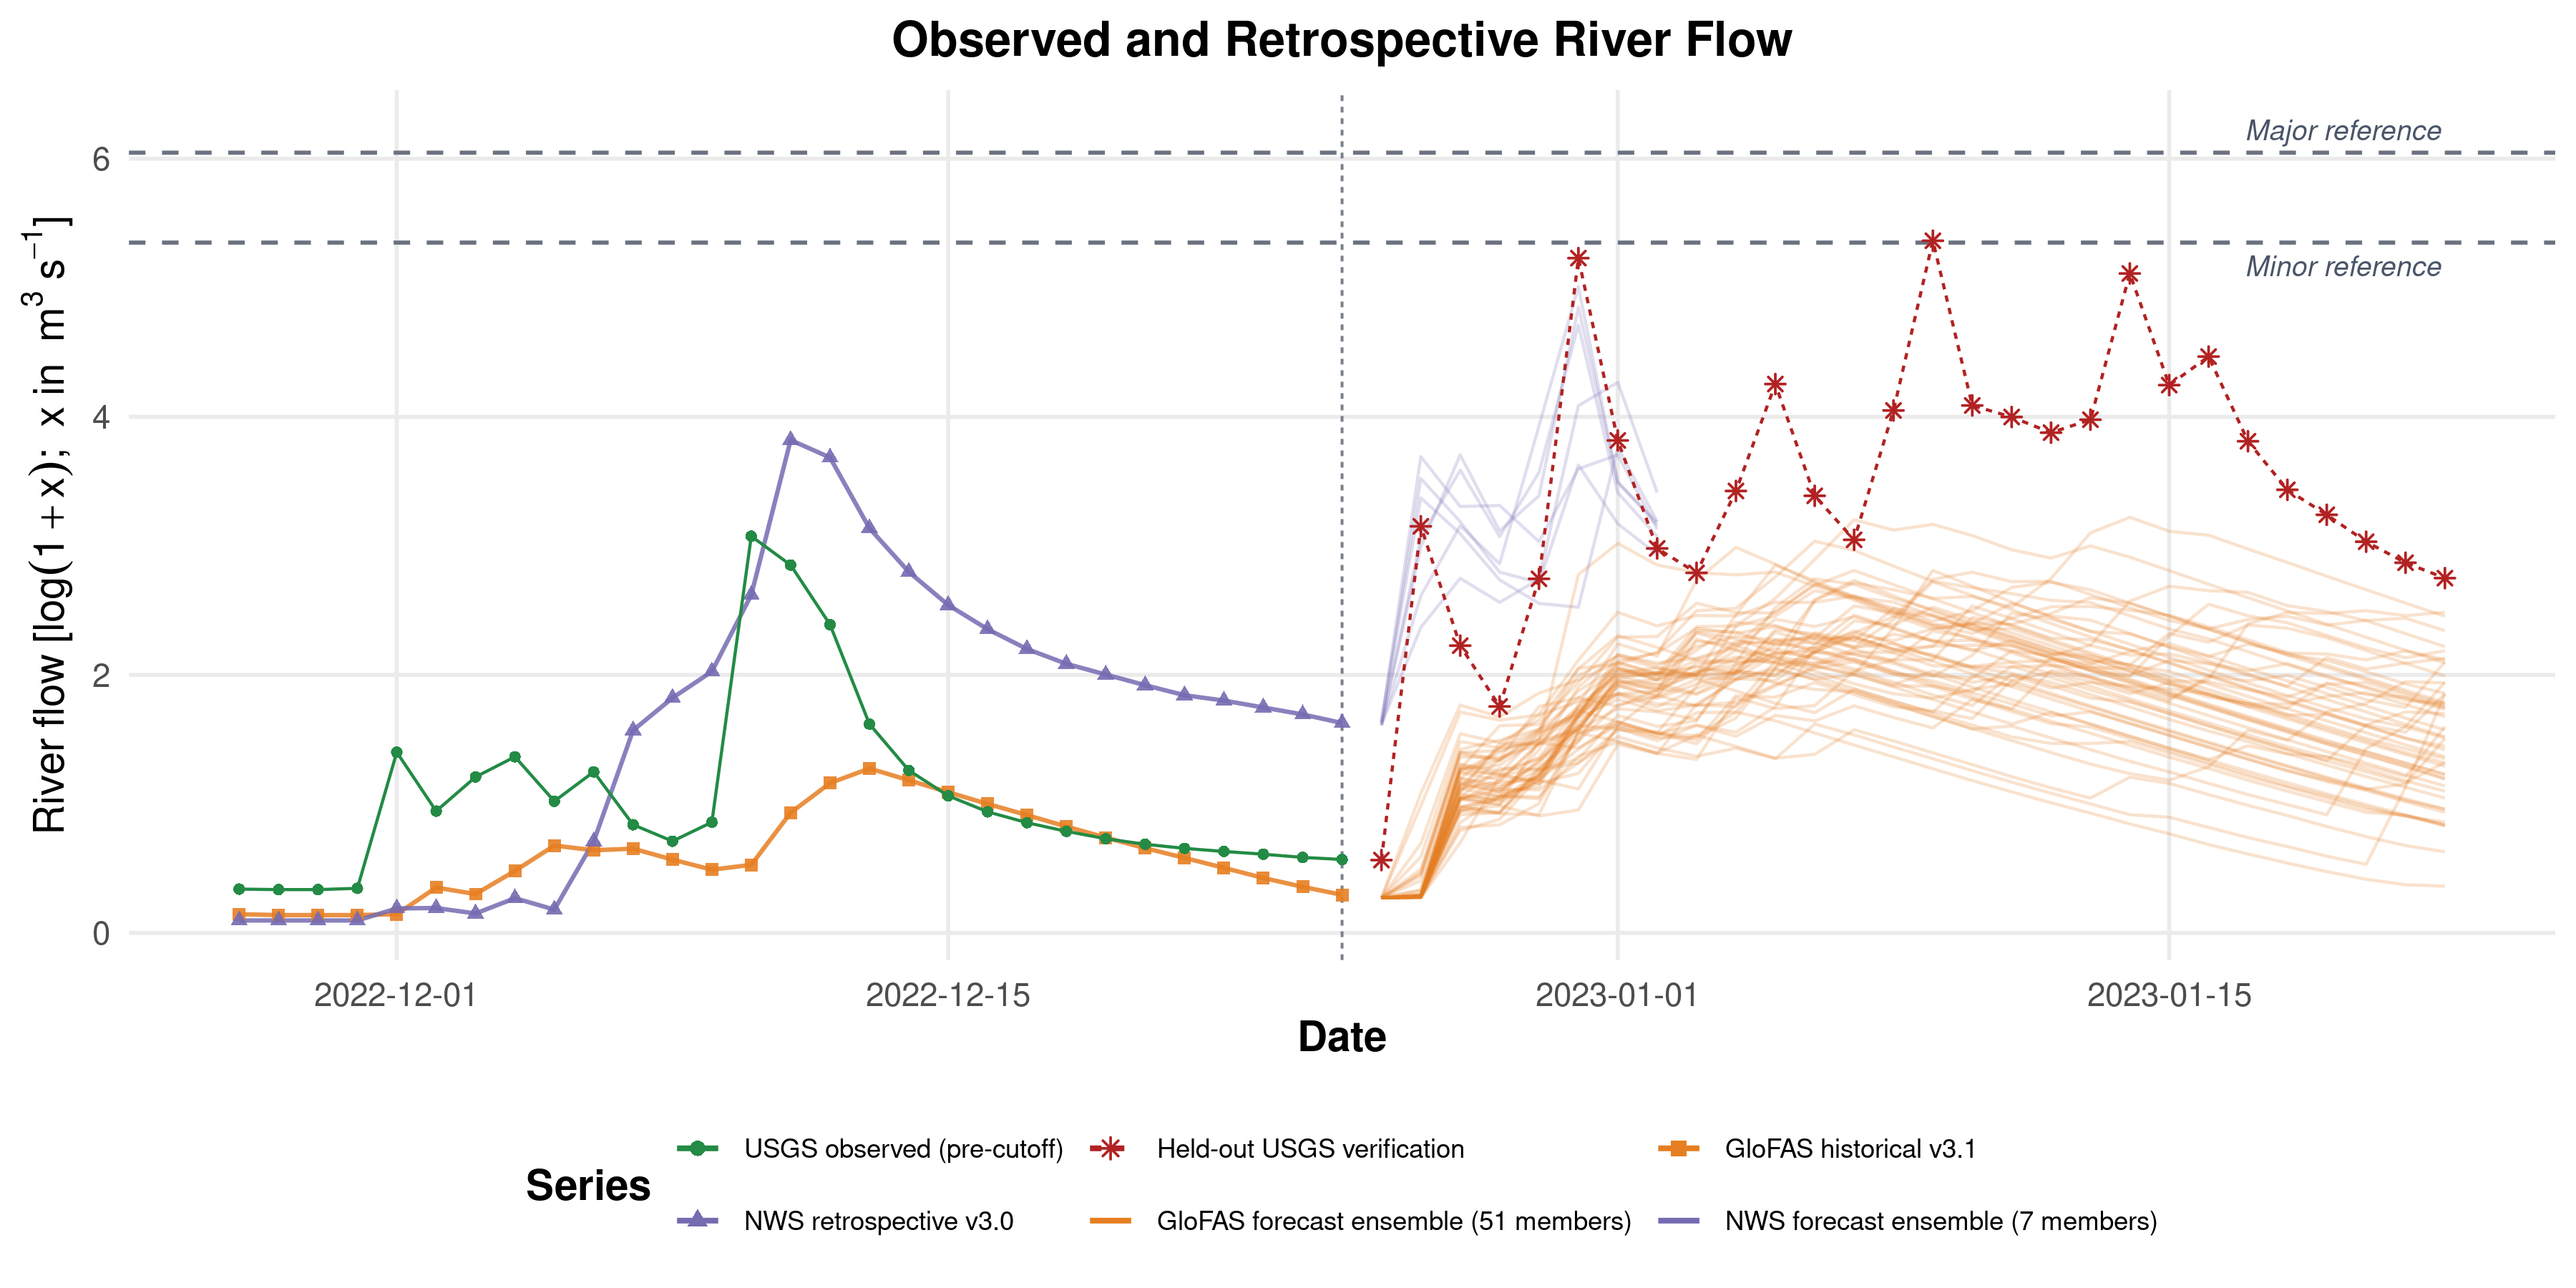
\includegraphics[width=\textwidth]{figures/ch03-environ/forecast_products_context.png}}
\caption{
Representative forecast-origin display for the December 25, 2022 cutoff, spanning November 27, 2022 through January 22, 2023 on the $\log(1+x)$ scale with $x$ in m$^3$/s. Before the cutoff, the panel shows USGS observations and the NWS and GloFAS retrospective products used for source-discrepancy learning; after the cutoff, it shows held-out USGS verification together with the operational NWS and GloFAS forecast ensembles. Horizontal dashed lines show approximate current-rating discharge equivalents of the current NWS minor and major stage categories at BTEC1/USGS 11160500; they are included as operational magnitude references rather than as historical flood-stage classifications.
}
\label{env:fig:ensembles}
\end{figure}

The chapter develops the modeling and inference framework before defining the
San Lorenzo data contract and the five-origin evaluation. Forecast validation
is followed by interpretation of the selected specification, sensitivity
analysis, and a final account of limitations and further work.

\section{Source-specific dynamic quantile model}
\label{env:sec:methodology}

Throughout the chapter, bold uppercase letters (e.g., $\mathbf{W}, \mathbf{F}, \mathbf{G}$) denote matrices, and bold lowercase letters (e.g., $\mathbf{x}, \boldsymbol{\psi}, \boldsymbol{\theta}$) denote vectors. We denote the identity matrix of dimension $r \times r$ as $\mathbf{I}_r$, a vector of zeros of dimension $r \times 1$ as $\mathbf{0}_r$, and a vector of ones of dimension $r \times 1$ as $\mathbf{1}_r$.

\subsection{Extended asymmetric Laplace likelihood}
\label{env:subsec:exal}

The use of the Asymmetric Laplace (AL) distribution for quantile inference within a Bayesian framework is well-established with both empirical and theoretical justifications \citep{env-yu2001bayesian,env-sriram2013theoretical}. We use the extended asymmetric Laplace (exAL) distribution, which addresses limitations of the AL working likelihood, particularly its restricted skewness. \citet{exd-yan2025family} proposed the exAL distribution, $\text{exAL}_{p_0}(\mu, \sigma, \gamma)$, where $\mu$ represents the $p_0$th quantile of interest, $\sigma$ is a positive scale parameter, and $\gamma$ is the skewness parameter. The parameter $\gamma$ has bounded support over the interval $(L, U)$, where $L$ is the negative root of $g(\gamma) = 1 - p_0$ and $U$ is the positive root of $g(\gamma) = p_0$, with $g(\gamma) = 2 \Phi(-|\gamma|) \exp(\gamma^2 / 2)$ and $\Phi$ denoting the standard normal cumulative distribution function. For computational implementation, we use the extended stochastic representation of an exAL random variable described in \citet{exd-yan2025family}. That is, if $y \sim \text{exAL}(\mu, \sigma, \gamma)$, then there exist independent random variables $\epsilon \sim \mathcal{N}(0, 1)$, $z \sim \text{Exp}(1)$, and $s \sim \mathcal{N}^+(0, 1)$, (where $\mathcal{N}^+(0, 1)$ denotes the standard normal distribution truncated to the positive real line), such that  \( y = \mu + C(\gamma; p_0)\sigma |\gamma| s + A(\gamma; p_0) \sigma z + \sqrt{B(\gamma; p_0) \sigma^2 z} \cdot \epsilon, \) where $A(\gamma; p_0) = \frac{1 - 2 p(\gamma; p_0)}{p(\gamma; p_0) \, [1 - p(\gamma; p_0)]}$, $B(\gamma; p_0) = \frac{2}{p(\gamma; p_0) \, [1 - p(\gamma; p_0)]}$, $C(\gamma; p_0) = [I(\gamma > 0) - p(\gamma; p_0)]^{-1}$, and $p(\gamma; p_0) = I(\gamma < 0) + \{p_0 - I(\gamma < 0)\} / g(\gamma)$.


\subsection{State-space model specification}
\label{env:subsec:fullmodel}

For a fixed target quantile $p_0$, we use a single state-space model whose latent process evolves across both the pre-cutoff observation period and the forecast horizon. The cutoff, denoted by \(T\), separates the data used for fitting from the post-cutoff observations reserved for verification. The latent river-flow quantile is represented by a trend-and-seasonal state \(\boldsymbol{\theta}_t \in \mathbb{R}^p\), observed through the loading vector \(\mathbf{F}_t\). Each external product family \(j\) has its own discrepancy state \(\boldsymbol{\delta}_t^j \in \mathbb{R}^p\), allowing that product to depart systematically from the observed river-flow series. A scalar transfer adjustment \(\zeta_t\) incorporates exogenous covariates \(\mathbf{x}_t \in \mathbb{R}^m\), whose time-varying effects are collected in \(\boldsymbol{\psi}_t \in \mathbb{R}^m\). Let \(\mathcal{J}=\{1,\ldots,J\}\) denote the set of external product families. For each \(j\in\mathcal{J}\), let \(\mathcal{I}_j=\{1,\ldots,I_j\}\) index forecast members and \(\mathcal{K}_j=\{1,\ldots,K_{(j)}\}\) index forecast lead times. Finally, define \(K_{\max}=\max_{j\in\mathcal{J}}K_{(j)}\), the maximum forecast horizon across all sources.

The expanded specification is:
\begingroup\scriptsize\begin{alignat}{3}
\text{Observed measurements:}\quad&
y_t^o
&\sim{}& \text{exAL}_{p_0}\!\left(\mathbf{F}_t' \boldsymbol{\theta}_t + \zeta_t, \sigma^0, \gamma^0\right),
&\qquad& 1 \le t \le T, \label{env:eq:unified_usgs}
\\
\text{Retrospective products:}\quad&
z_t^j
&\sim{}& \text{exAL}_{p_0}\!\left(\mathbf{F}_t'(\boldsymbol{\theta}_t + \boldsymbol{\delta}_t^j) + \zeta_t, \sigma^j, \gamma^j\right),
&\qquad& j \in \mathcal{J},\ 1 \le t \le T, \label{env:eq:unified_retro}
\\
\text{Forecast products:}\quad&
y_T^{j,i}(k)
&\sim{}& \text{exAL}_{p_0}\!\left(\mathbf{F}_{T+k}'(\boldsymbol{\theta}_{T+k} + \boldsymbol{\delta}_{T+k}^j) + \zeta_{T+k}, \sigma^j, \gamma^j\right),
&\qquad& j \in \mathcal{J},\ i \in \mathcal{I}_j,\ k \in \mathcal{K}_j, \notag
\\
\text{Trend and seasonal states:}\quad&
\boldsymbol{\theta}_t \mid \boldsymbol{\theta}_{t-1}
&\sim{}& \mathcal{N}\!\left(\mathbf{G}_t \boldsymbol{\theta}_{t-1}, \mathbf{W}_t^\theta\right),
&\qquad& 1 \le t \le T+K_{\max}, \label{env:eq:unified_theta}
\\
\text{Discrepancy states:}\quad&
\boldsymbol{\delta}_t^j \mid \boldsymbol{\delta}_{t-1}^j
&\sim{}& \mathcal{N}\!\left(\mathbf{G}_t \boldsymbol{\delta}_{t-1}^j, \mathbf{W}_t^{\delta^j}\right),
&\qquad& j \in \mathcal{J},\ 1 \le t \le T+K_{\max}, \label{env:eq:unified_delta}
\\
\text{Transfer adjustment:}\quad&
\zeta_t \mid \zeta_{t-1}, \boldsymbol{\psi}_{t-1}
&\sim{}& \mathcal{N}\!\left(\lambda \zeta_{t-1} + \mathbf{x}_t'\boldsymbol{\psi}_{t-1}, w_t^\zeta\right),
&\qquad& 1 \le t \le T+K_{\max}, \label{env:eq:unified_transfer}
\\
\text{Covariate-effect states:}\quad&
\boldsymbol{\psi}_t \mid \boldsymbol{\psi}_{t-1}
&\sim{}& \mathcal{N}\!\left(\boldsymbol{\psi}_{t-1}, \mathbf{W}_t^\psi\right),
&\qquad& 1 \le t \le T+K_{\max}. \notag
\end{alignat}\endgroup

Here \(\mathbf{F}_t \in \mathbb{R}^{p}\), \(\mathbf{G}_t \in \mathbb{R}^{p\times p}\), \(\mathbf{W}_t^\theta \in \mathbb{R}^{p\times p}\), \(\mathbf{W}_t^{\delta^j} \in \mathbb{R}^{p\times p}\), \(\mathbf{W}_t^\psi \in \mathbb{R}^{m\times m}\), and \(w_t^\zeta \in \mathbb{R}_+\) is the scalar evolution variance for the transfer state \(\zeta_t\). The parameter \(\lambda \in \mathbb{R}\) governs persistence in the transfer adjustment, while \(\mathbf{x}_t'\boldsymbol{\psi}_{t-1}\) is the covariate contribution at time \(t\). During the forecast window, \(\mathbf{x}_{T+k}\) denotes the forecast-window covariate vector available from the staged cutoff-specific input bundle. The notation \(y_T^{j,i}(k)\) denotes the \(k\)-step-ahead forecast issued at time \(T\) by member \(i\) of source \(j\).

The first two observation equations correspond to the pre-cutoff observation window, where the available channels are the observed USGS flow and the retrospective products. The third observation equation corresponds to the forecast window, where issued forecast products enter through the same source-specific discrepancy structure. The state-evolution equations define the roles of the dynamic components: \(\boldsymbol{\theta}_t\) carries the river-flow level and seasonal structure, \(\boldsymbol{\delta}_t^j\) captures systematic source-specific departures from the observations, and the transfer component maps exogenous covariates into the quantile process through \(\zeta_t\) and \(\boldsymbol{\psi}_t\).

Define
\[
\boldsymbol{\omega}_t' = [\zeta_t,\ \boldsymbol{\psi}_t'], \qquad
\boldsymbol{\eta}_t' = [\boldsymbol{\theta}_t',\ (\boldsymbol{\delta}_t^1)',\ \ldots,\ (\boldsymbol{\delta}_t^J)',\ \boldsymbol{\omega}_t'],
\]
where \(\boldsymbol{\omega}_t \in \mathbb{R}^{m+1}\) and \(\boldsymbol{\eta}_t \in \mathbb{R}^{q}\), with \(q = (J+1)p + m + 1\). The transfer update can be written as
\[
\mathbf{G}^{\text{trans}}_t =
\begin{bmatrix}
\lambda & \mathbf{x}_t' \\
\mathbf{0}_m & \mathbf{I}_m
\end{bmatrix}.
\]
Let \(\mathcal{J}_0=\{0\}\cup\mathcal{J}\), where \(s=0\) denotes the USGS observation channel and \(s\in\mathcal{J}\) denotes an external product family. Let \(y_t^0 \equiv y_t^o\) denote the observation channel and \(y_t^s \equiv z_t^s\), \(s\in\mathcal{J}\), denote the retrospective-product channels. The corresponding compact form is:
\begingroup\scriptsize\begin{alignat}{3}
\text{Pre-cutoff observations:}\quad&
y_t^s \mid \boldsymbol{\eta}_t, \sigma^s, \gamma^s
&\sim{}& \text{exAL}_{p_0}\!\left(\mathbf{h}_{t,s}' \boldsymbol{\eta}_t, \sigma^s, \gamma^s\right),
&\qquad& 1 \le t \le T,\ s \in \mathcal{J}_0, \label{env:eq:compact_est_obs}
\\
\text{Pre-cutoff state evolution:}\quad&
\boldsymbol{\eta}_t \mid \boldsymbol{\eta}_{t-1}
&\sim{}& \mathcal{N}\!\left(\boldsymbol{D}_t \boldsymbol{\eta}_{t-1}, \boldsymbol{\Lambda}_t\right),
&\qquad& 1 \le t \le T, \label{env:eq:compact_est_state}
\\
\text{Forecast observations:}\quad&
y_T^{j,i}(k) \mid \boldsymbol{\eta}_{T+k}, \sigma^j, \gamma^j
&\sim{}& \text{exAL}_{p_0}\!\left(\mathbf{e}_{T+k,j}' \boldsymbol{\eta}_{T+k}, \sigma^j, \gamma^j\right),
&\qquad& j \in \mathcal{J},\ i \in \mathcal{I}_j,\ k \in \mathcal{K}_j, \label{env:eq:compact_fc_obs}
\\
\text{Forecast state evolution:}\quad&
\boldsymbol{\eta}_{T+k} \mid \boldsymbol{\eta}_{T+k-1}
&\sim{}& \mathcal{N}\!\left(\boldsymbol{M}_{T+k} \boldsymbol{\eta}_{T+k-1}, \mathbf{W}_{T+k}\right),
&\qquad& 1 \le k \le K_{\max}. \label{env:eq:compact_fc_state}
\end{alignat}\endgroup

Here
\begingroup\scriptsize\[
\big(\mathbf{F}_t^{\text{trans}}\big)' = [1,\ \mathbf{0}_m'], \qquad
\mathbf{h}_{t,0}' =
\big[\mathbf{F}_t',\ \mathbf{0}_{pJ}',\ \big(\mathbf{F}_t^{\text{trans}}\big)'\big],
\qquad
\mathbf{h}_{t,j}' =
\big[\mathbf{F}_t',\ \mathbf{0}_{p(j-1)}',\ \mathbf{F}_t',\ \mathbf{0}_{p(J-j)}',\ \big(\mathbf{F}_t^{\text{trans}}\big)'\big],
\quad j \in \mathcal{J},
\]\endgroup
with \(\mathbf{F}_t^{\text{trans}} \in \mathbb{R}^{m+1}\), \(\mathbf{h}_{t,0}, \mathbf{h}_{t,j} \in \mathbb{R}^{q}\), and
\[\resizebox{\textwidth}{!}{$\displaystyle
\boldsymbol{D}_t = \text{BlockDiag}\!\left(\mathbf{G}_t,\ \underbrace{\mathbf{G}_t,\ldots,\mathbf{G}_t}_{J\ \text{discrepancy blocks}},\ \mathbf{G}^{\text{trans}}_t\right), \qquad
\boldsymbol{\Lambda}_t = \text{BlockDiag}\!\left(\mathbf{W}^{\theta}_t,\ \underbrace{\mathbf{W}^{\delta^1}_t,\ldots,\mathbf{W}^{\delta^J}_t}_{J\ \text{source-specific discrepancy blocks}},\ \text{BlockDiag}\!\left(w_t^{\zeta}, \mathbf{W}^{\psi}_t\right)\right),
$}\]
where \(\boldsymbol{D}_t, \boldsymbol{\Lambda}_t \in \mathbb{R}^{q\times q}\) and \(\sigma^s \in \mathbb{R}_+\), \(\gamma^s \in \mathbb{R}\) denote the channel-specific scale and skewness parameters for \(s \in \mathcal{J}_0\). Thus, \(\mathbf{h}_{t,0}' \boldsymbol{\eta}_t = \mathbf{F}_t' \boldsymbol{\theta}_t + \zeta_t\) and \(\mathbf{h}_{t,j}' \boldsymbol{\eta}_t = \mathbf{F}_t'(\boldsymbol{\theta}_t + \boldsymbol{\delta}_t^j) + \zeta_t\). For the forecast window, \(\mathbf{e}_{T+k,j}\) is the analogue of \(\mathbf{h}_{t,j}\): it extracts the latent trend-and-seasonal block, the discrepancy block for source \(j\), and the transfer block. The matrices \(\boldsymbol{M}_{T+k}\) and \(\mathbf{W}_{T+k}\) preserve the same block ordering while propagating the active forecast-window state.

This compact representation highlights the conditionally Gaussian state-space structure induced by the stochastic representation in Subsection~\ref{env:subsec:exal}. The observation equations are conditionally Gaussian given the latent augmentation variables, and the state evolution remains Gaussian. The model can therefore be handled with standard state-space methods, including filtering, smoothing, and sampling recursions.

\subsection{Prior specification and discounting}
\label{env:subsec:prioranddisc}
To complete the model we specify prior distributions for the initial states, the scale, and skewness parameters.
Following \citet{exd-me}, for each channel-specific skewness parameter, we assign a truncated Student-\(t\) prior:
\[
\gamma^s \sim t_{(L,U)}(0,\phi^s,\nu^s), \qquad s\in\mathcal{J}_0,
\]
where \(\phi^s\) and \(\nu^s\) denote the scale and degrees of freedom hyperparameters, respectively. For the channel-specific scale parameters, we use inverse-gamma priors,
\[
\sigma^s \sim IG(a_{\sigma^s}, b_{\sigma^s}), \qquad s\in\mathcal{J}_0,
\]
with \(a_{\sigma^s}\) and \(b_{\sigma^s}\) as shape and scale hyperparameters. The full latent state is initialized as \(\boldsymbol{\eta}_0 \sim \mathcal{N}(\mathbf{m}_0, \mathbf{C}_0)\), with \(\mathbf{m}_0 \in \mathbb{R}^{q}\) and \(\mathbf{C}_0 \in \mathbb{R}^{q\times q}\). This initial prior covers the shared trend-and-seasonal quantile block, the source-specific discrepancy blocks, and the transfer block.

Discount factors \citep{env-prado2021time} are used for adaptive evolution of the covariance matrices at the state level. Discount factors lie in the $(0,1]$ range, with 1 indicating no dynamic evolution and smaller values implying greater temporal adaptability. We use component discounting. The application-specific choices are given in Subsection~\ref{env:subsec:specification}. During the forecast window ($t \in \{T+1, \ldots, T+K_{\max}\}$), we set the Inverse Wishart prior parameters as $\mathbf{S}_t = (\nu_t - p_t - 1)\, c\, \mathbf{W}_T$ and $\nu_t = (p_t + 1 + \epsilon)$, with $\epsilon, c > 0$, where \(p_t\) denotes the dimension of the active forecast-window state at time \(t\), \(\mathbf{S}_t \in \mathbb{R}^{p_t\times p_t}\), and \(\mathbf{W}_T \in \mathbb{R}^{p_t\times p_t}\) after restricting the full pre-cutoff covariance to the active forecast-window block. Under this specification, the posterior mean is
\(
\mathbb{E}[\mathbf{W}_t \mid \mathcal{D}_t] = \frac{\epsilon}{1 + \epsilon}(c\, \mathbf{W}_T) + \frac{1}{1 + \epsilon} \mathbb{E}\left[ (\boldsymbol{\eta}_t - \mathbf{M}_t \boldsymbol{\eta}_{t-1}) (\boldsymbol{\eta}_t - \mathbf{M}_t \boldsymbol{\eta}_{t-1})' \mid \mathcal{D}_t \right],
\)
where $\mathcal{D}_t$ denotes all data available up to and including time $t$.

This posterior mean is a convex combination of two terms: the covariance learned before the cutoff, carried forward through \(c\mathbf{W}_T\), and the forecast-window residual covariance implied by the propagated state. The scalar \(c\) controls the scale of the carried-forward covariance anchor, while \(\epsilon\) controls how strongly that anchor is retained. In the reported analysis we use this prior as a short-horizon stabilization device: it prevents the forecast-window covariance from being driven entirely by a small number of post-cutoff forecast-product updates, while still allowing the forecast-window state evolution to adapt through the second term in the convex combination.
Further details regarding prior specification and discount factors are provided in Subsection~\ref{env:subsec:specification}.

\subsection{Posterior computation}
\label{env:subsec:postinf}
Initially, we explored the posterior distribution of all model parameters using a Markov chain Monte Carlo (MCMC) algorithm.
Algorithm~\ref{env:alg1} gives the core MCMC updates in a compact source-indexed notation. As indicated by Equation~\ref{env:eq:compact_est_obs}, during the pre-cutoff observation window the response variables are the USGS observations and retrospective products. After the cutoff, Equation~\ref{env:eq:compact_fc_obs} applies and the response variables correspond to the forecast products. Careful bookkeeping is needed because forecast horizons differ across agencies. Gibbs sampling is facilitated by the fact that all full posterior conditionals are available in closed form except for the channel-specific skewness parameters \(\gamma^s\), \(s\in\mathcal{J}_0\). For these, we use a Metropolis--Hastings random walk on an unconstrained reparameterization. Posterior sampling of the state parameters relies on a modified Forward Filtering Backward Sampling (FFBS) algorithm that leverages their conditional normality (see Algorithm~\ref{env:alg:Alg2}).

%\subsubsection{Variational Bayes Implementation} \label{env:subsec:vb}

Given the computational demands of traditional Markov Chain Monte Carlo (MCMC) methods on large datasets, we also implement a Mean Field Variational Bayes (MFVB) algorithm to approximate posterior inference.
\citet{exd-me} proposed a Variational Bayes algorithm that embeds an importance sampling scheme for non-conjugate parameters; however, this scheme risks particle collapse in high dimensions and requires further constraints to avoid degeneracy. In particular, it fixes the scale parameter of the exAL using pre-estimated values from an AL model.
Building on \citet{exd-me}, we address stability issues in their importance-sampling approximation by adopting the variational Bayes Laplace--delta (VB--LD) method of \citet{exd-wang2013nonconjugatevb}. A Laplace approximation handles the low-dimensional nonconjugate block, and delta-method expansions approximate its moments in the remaining coordinate updates.

Let \(\boldsymbol{\alpha}\) denote the nonconjugate scale--skewness
parameters and \(\boldsymbol{\beta}\) the remaining quantities. Under the
mean-field factorization
\(q(\boldsymbol{\alpha},\boldsymbol{\beta})
=q(\boldsymbol{\alpha})q(\boldsymbol{\beta})\), the conjugate blocks retain
closed-form coordinate updates. For
\(\ell(\boldsymbol{\alpha})
=\mathbb{E}_{q(\boldsymbol{\beta})}\{\log
p(D,\boldsymbol{\alpha},\boldsymbol{\beta})\}\), VB--LD uses
\[
q(\boldsymbol{\alpha})
\approx \mathcal N(\widehat{\boldsymbol{\alpha}},\Sigma),\qquad
\widehat{\boldsymbol{\alpha}}=\arg\max\ell(\boldsymbol{\alpha}),\quad
\Sigma=-\{\nabla^2\ell(\widehat{\boldsymbol{\alpha}})\}^{-1}.
\]
Second-order delta expansions provide the moments of
\(q(\boldsymbol{\alpha})\) required by the conjugate updates. The algorithm
alternates these steps until the monitored evidence lower bound stabilizes.
Appendix~\ref{app:hydrology-technical} gives the complete update equations and
implementation pseudocode.

Our approach fits a separate state-space model for each target quantile level, which allows the seven quantile-specific models used in the application to be fitted in parallel. In the San Lorenzo application, the full quantile set can be refit once observations, retrospective products, forecast products, and forecast covariates have been staged; the recorded runs take about two hours end-to-end on a Linux server with 64 cores and 503 GiB of RAM. These timings use the practical runtime fields \texttt{runtime\_sec\_total} and \texttt{runtime\_sec}; they are combined wall-clock measurements because fitting and forecasting were not timed separately, and they are hardware- and implementation-dependent. The main computational cost arises from repeated filtering and smoothing operations and increases with the length of the time series and the dimension of the latent state. These recorded timings do not establish an operational deployment claim.

\subsection{Posterior predictive synthesis across quantiles}
\label{env:subsec:quantilesynthesis}

The model is fitted separately at a finite set of target quantile levels, but forecast validation and visualization require a single predictive distribution at each time point. Because independently fitted quantile models do not automatically define one monotone predictive quantile function, we apply a post-fit synthesis step to the posterior predictive output from the fitted quantile-specific models. This step uses only posterior predictive output from the fitted models: it does not refit the state-space models, alter the VB updates, or use held-out post-cutoff USGS observations.

Let \(0<\tau_1<\cdots<\tau_L<1\) denote the fitted quantile levels and let \(Y_{\ell,t}^{(r)}\) be posterior predictive draws from the model fitted at level \(\tau_\ell\), for \(r=1,\ldots,R\). Let \(q_{\ell,t}\) be the empirical \(\tau_\ell\)-quantile of those draws. Because the \(L\) quantile models are fitted independently, the anchor values \(q_{\ell,t}\) are first adjusted with isotonic regression \citep{exd-barlow1972},
\[
\mathbf{m}_t^*
= \underset{m_1 \leq \cdots \leq m_L}{\arg\min}
\sum_{\ell=1}^L (q_{\ell,t}-m_\ell)^2 .
\]
The posterior draws from each quantile lane are then shifted to match the adjusted anchor,
\[
Y_{\ell,t}^{(r),\mathrm{adj}}
= Y_{\ell,t}^{(r)} + (m_{\ell,t}^* - q_{\ell,t}).
\]
The adjusted quantile anchors define an initial synthesized quantile curve by interpolation across adjacent fitted levels. We evaluate this curve on a dense probability grid and apply monotone rearrangement \citep{exd-chernozhukov2010} to obtain a nondecreasing synthesized quantile function \(\widetilde Q_t\). This step reduces the risk of quantile crossing after independently fitting the quantile-specific models. Evaluating the rearranged quantile function on \(u_r=r/(R+1)\), \(r=1,\ldots,R\), gives the synthesized empirical posterior predictive sample
\[
z_t^{(r)}=\widetilde Q_t(u_r).
\]
The sample \(\{z_t^{(r)}:r=1,\ldots,R\}\) is the per-time marginal predictive distribution used for the displayed synthesis bands, posterior predictive quantiles, and CRPS calculations.

\subsection{Predictive scoring by CRPS}
\label{env:subsec:modelselection}

For predictive scoring, we use the Continuous Ranked Probability Score (CRPS) \citep{exd-gneiting2007} as the primary score for forecast-window predictive distributions and, separately, as a preliminary calibration criterion for selected specification choices. The CRPS is negatively oriented, so smaller values are better, and it is a proper score for predictive distributions that rewards both calibration and sharpness.

For a predictive distribution \(G\) with quantile function \(Q_G\) and an observation \(y\), the CRPS is defined as
\[
\text{CRPS}(y, G) = 2 \int_0^1 \rho_u\!\left(y - Q_G(u)\right)\, du,
\qquad
\rho_u(v) = v\big(u - \mathbf{1}\{v<0\}\big),
\]
where \(\rho_u\) is the quantile score, or check loss. Thus, the CRPS is a natural score in the context of quantile estimation. For a generic empirical predictive distribution represented by sample values \(z_t^{(1)},\ldots,z_t^{(S)}\), we approximate the integral by evaluating the empirical quantile function on the grid \(u_s=s/(S+1)\), \(s=1,\ldots,S\). Let \(z_{t,(1)} \leq \cdots \leq z_{t,(S)}\) be the corresponding ordered sample values. Then
\[
\widehat{\mathrm{CRPS}}(y_t,G_t)
= \frac{2}{S}\sum_{s=1}^S
\rho_{u_s}\!\left(y_t-z_{t,(s)}\right).
\]
The same calculation is used for synthesized posterior predictive samples and for raw forecast ensembles, with \(S\) equal to the number of available sample draws or ensemble members at that lead. If the predictive distribution is a point mass at \(x\), the CRPS reduces to \(|y-x|\); averaging this quantity across forecast cases gives the mean absolute error. CRPS is also used in the preliminary pre-cutoff calibration of the transfer-persistence parameter \(\lambda\), as described in Subsection~\ref{env:subsec:specification}.

\section{Computational implementation}
\label{environ:sec:body-computation}

Inference is carried out with the MCMC and variational procedures induced by
the source-aware state-space model.  Both approaches preserve the distinction
between the response process, source-specific latent quantities, and the
subsequent synthesis across quantile levels.  The empirical comparisons below
therefore evaluate a fixed model-and-algorithm contract rather than a generic
post-processing rule.

The complete full-conditionals, filtering and smoothing recursions, and
stepwise MCMC and VB algorithms appear in
Appendix~\ref{app:hydrology-technical}.

\section{San Lorenzo River application}
%\section{APPLICATION DATA AND FORECASTING DESIGN}
\label{env:sec:data}

\subsection{Study setting and observations}

Our target series is the average daily natural water flow of the San Lorenzo River at the Big Trees U.S. Geological Survey (USGS) gauging station in Santa Cruz, California (Figure \ref{env:fig:sanlorenzo}). The raw USGS discharge record is reported in cubic feet per second; we convert it to m$^3$/s before applying the $\log(1+x)$ transformation used in the figures and model inputs. The Big Trees location is characterized by minimal human intervention, so the recorded flow closely reflects natural river dynamics. Over the study window used in this chapter, the daily series covers May 29, 1987, through December 25, 2022, and contains 12,995 observations.
The San Lorenzo River is a major water resource for the Santa Cruz area and is relevant to both flood response and longer-term water-supply planning. The record includes high-flow episodes as well as prolonged dry conditions. The analysis and forecasting of lower quantiles are therefore relevant for drought conditions, whereas upper quantiles are relevant for flood risk.

\begin{figure}[htbp]
\centering
\includegraphics[width=\textwidth]{figures/ch03-environ/site_context_usgs.png}
\caption{
Observed USGS daily water flow on the $\log(1 + x)$ scale, with $x$ measured in m$^3$/s, May 29, 1987 through December 25, 2022. Horizontal dashed lines show approximate current-rating discharge equivalents of the current NWS minor and major stage categories at BTEC1/USGS 11160500, computed from USGS stage-discharge rating 40.0 and transformed to the plotting scale \citep{env-cnrfc_btec1,env-usgs_11160500_rating40}. They are operational magnitude references for the discharge scale, not historical flood-stage classifications of daily-mean observations.
}
\label{env:fig:sanlorenzo}
\end{figure}

We combine the USGS observations with three additional information sources: forecast covariates, retrospective products, and forecast products. Each source plays a different role. The covariates enter the transfer component of the latent process, the retrospective products are used to learn source-specific discrepancies over the pre-cutoff observation window, and the forecast products inform the post-cutoff predictive distributions.

\subsection{External data sources and forecast covariates}

The transfer component takes three inputs: local precipitation from the PRISM Climate Group \citep{env-prism}, local soil moisture from ECMWF ERA5-Land \citep{env-ecmwf}, and a low-dimensional summary of broader climate conditions. Pre-cutoff precipitation and soil moisture are historical gridded covariates extracted at the Big Trees location. After the cutoff, the forecast-window precipitation and soil-moisture covariates are based on Global Ensemble Forecast System (GEFS) precipitation and shallow soil-water forecasts staged in the cutoff-specific origin bundle. These local hydrometeorological covariates enter as deterministic summaries in the present implementation. Precipitation is not modeled through a separate censoring, zero-inflation, or occurrence/intensity layer; dry days are retained in the supplied covariate path, and precipitation contributes through external transfer covariates and deterministic engineered terms. The ERA5-Land soil-moisture series is one of the reanalysis-based model inputs rather than direct observations or uncertainty-free measurements. ERA5/ERA5-Land variables may include short forecast components, but in this analysis they are covariates, not verification observations.

The broader climate summary is constructed from monthly climate and environmental indices from \citet{env-noaa_climate_indices}, including solar flux, Niño 1+2, the Oceanic Niño Index (ONI), the Southern Oscillation Index (SOI), the Western Hemisphere Warm Pool (WHWP), the Global Mean Temperature (GMT), the Northern Oscillation Index (NOI), the Atlantic Multidecadal Oscillation (AMO), and the Tropical South (TSA) and North Atlantic (TNA) indices. These series are interpolated to daily resolution to align with the hydrological data. We summarize the standardized index matrix with the first generalized dynamic principal component (GDPC) \citep{env-JSSv092c02}, which explains 44.07\% of the total variability. The GDPC factor is treated as a climate-index covariate, not as an operational forecast product or verification target. Figure~\ref{env:fig:covariates} shows these three explanatory series.

\begin{figure}[hbt!]
\centering
\centerline{\includegraphics[width=\textwidth]{figures/ch03-environ/covariate_context_precip_soil_gdpc.png}}
\caption{
Historical daily precipitation [mm], soil moisture [m$^3$/m$^3$], and first GDPC score over May 29, 1987 through December 25, 2022.}
\label{env:fig:covariates}
\end{figure}

The external product families come from two agencies: GloFAS, operated by ECMWF, and NWS/National Water Model products from NOAA \citep{env-cosgrove2024noaa}. Each agency contributes both retrospective information and operational forecast information. The retrospective products are useful because they provide historically aligned external series that can be compared against the target observations before the cutoff, allowing the model to learn source-specific discrepancy patterns before those same sources enter the forecast window. The retrospective products enter the pre-cutoff observation window and are used to learn source-specific discrepancies relative to the USGS target series. Figure~\ref{env:fig:retrospectives} shows the corresponding retrospective series over the available pre-cutoff support window for the December 25, 2022 cutoff.

These products also differ in spatial support. For gridded covariates and GloFAS discharge fields, the analysis uses the cell or nearest valid river cell associated with the Big Trees gauge coordinates. For NWM streamflow, it uses the corresponding model-output point or reach series and aggregates the latest available forecast issuances to daily member-specific forecast matrices. The PRISM precipitation path uses the 4 km product, while ERA5-Land soil moisture is extracted from its 0.1-degree gridded product. The GloFAS retrospective series are version-specific over the study period, with the retrospective version and extraction policy fixed for each cutoff.

The operational forecast products are used only after a cutoff date. The NWS ensemble has 7 members: 6 members provide medium-range forecasts up to 8.5 days, and one control member extends to 10 days. The GloFAS ensemble contains 51 members, all providing medium-range forecasts for up to 28 days. These products therefore differ not only in source but also in forecast horizon and operational update pattern, which is why the forecast window must be modeled source by source rather than as a single homogeneous input stream.

\begin{figure}[hbt!]
\centering
\centerline{\includegraphics[width=\textwidth]{figures/ch03-environ/retrospective_products_context.png}}
\caption{Selected GloFAS and NWS retrospective product series over the available pre-cutoff support window for the December 25, 2022 cutoff, May 29, 1987 through December 25, 2022. Displayed flow values use the $\log(1+x)$ scale with $x$ in m$^3$/s.}
\label{env:fig:retrospectives}
\end{figure}

\subsection{Model specification}
%\subsection{Application-Specific Model Specification}
\label{env:subsec:specification}

For the San Lorenzo application, the latent quantile process combines a local level, three seasonal harmonics, and the transfer component defined in Section~\ref{env:sec:methodology}. The source-specific discrepancy states use the same trend-and-seasonal backbone. The trend-and-seasonal state has dimension \(p=7\). The matrix \(\mathbf{G}_t\) is composed of a trend component and a seasonal component. For the trend component, we include a constant term to represent the long-term average level of the quantile of interest. This component is defined by the evolution matrix and observational vector:
\( \mathbf{G}^{\text{trend}}_t = [1] \in \mathbb{R}^{1\times1}, \quad
\mathbf{F}^{\text{trend}}_t = [1] \in \mathbb{R}^{1}. \) The seasonal component incorporates three harmonics identified through exploratory spectral analysis of the full development record: an annual harmonic (12 months), a semiannual harmonic (6 months), and a long-term harmonic with an approximately 82-month (6.81-year) cycle that captures cyclical behavior associated with alternating phases of heavy rainfall and prolonged drought. Like the globally selected transfer persistence, these frequencies are part of the retrospective specification and are not reselected within each origin. The seasonal component's evolution matrix and observational vector are defined as:
\( \mathbf{G}^{\text{seas}}_t = \text{BlockDiag}\left(\textbf{J}_2(1,1),\ \textbf{J}_2(1,2),\ \textbf{J}_2\left(1,\frac{1}{6.8068493}\right)\right),\quad
\mathbf{F}^{\text{seas}}_t  =
\begin{bmatrix}
\mathbf{E}_2 \\[5pt]
\mathbf{E}_2 \\[5pt]
\mathbf{E}_2
\end{bmatrix}, \)
where
\( \textbf{J}_2(1,\omega) =
\begin{bmatrix}
\cos(\omega) & \sin(\omega) \\[5pt]
-\sin(\omega) & \cos(\omega)
\end{bmatrix},\quad
\mathbf{E}_2 =
\begin{bmatrix}
1 \\[5pt]
0
\end{bmatrix}. \)
Here \(\textbf{J}_2(1,\omega) \in \mathbb{R}^{2\times2}\), \(\mathbf{G}^{\text{seas}}_t \in \mathbb{R}^{6\times6}\), \(\mathbf{F}^{\text{seas}}_t \in \mathbb{R}^{6}\), and \(\mathbf{E}_2 \in \mathbb{R}^{2}\). Combining both components, the complete evolution matrix and observational vector for trend and seasonal dynamics become:
\(
\mathbf{G}_t = \text{BlockDiag}\left(\mathbf{G}^{\text{trend}}_t,\ \mathbf{G}^{\text{seas}}_t\right),\quad
\mathbf{F}_t =
\begin{bmatrix}
\mathbf{F}^{\text{trend}}_t \\[5pt]
\mathbf{F}^{\text{seas}}_t
\end{bmatrix}.
\) Thus, \(\mathbf{G}_t \in \mathbb{R}^{7\times7}\) and \(\mathbf{F}_t \in \mathbb{R}^{7}\).

For prior hyperparameters (see Subsection~\ref{env:subsec:prioranddisc}), we specify \(\phi^s = 10^6\), \(\nu^s = 1\), and \(a_{\sigma^s} = b_{\sigma^s} = 10^{-6}\) for all \(s\in\mathcal{J}_0\). These are small shape and scale hyperparameters for the channel-specific variance priors; they should not be interpreted as a general claim of prior noninformativeness. Sensitivity analyses for \(\phi^s \in \{10^1, 10^3, 10^6\}\) and \(b_{\sigma^s} \in \{10^{-1}, 10^{-3}, 10^{-6}\}\) showed no noticeable impact on model fit.

We choose discount factors componentwise to reflect each component's time scale and role. Recall that, in the discount-factor formulation \citep{env-prado2021time}, a smaller value \(d \in (0,1]\) for a given state parameter implies larger state-evolution variance and therefore greater adaptability of that component. The selected specifications use high, near-one discount factors for the trend, seasonal, discrepancy, transfer, and covariate-effect states. These values preserve persistent long-run behavior while allowing slow adaptation across the multi-decade observation window.

The transfer-persistence parameter \(\lambda\) was selected in a preliminary one-dimensional calibration step for the selected exAL-M-T1 specification. To avoid confounding transfer persistence with state-evolution adaptability, the component discount factors were held fixed during this step. We considered the grid \(\lambda \in \{0.60,0.61,\ldots,0.99\}\) and compared candidate values using CRPS for the median-quantile model over the pre-cutoff observational window at the representative December 25, 2022 cutoff, which has the longest pre-origin archive among the retained cases. The selected value was \(\lambda=0.97\), which was then held fixed across the reported quantile levels and forecast origins. Because this global specification used information extending through the 2022 representative origin, its use at earlier origins is retrospective rather than a strict pseudo-operational hindcast. The forecast-window outcomes remain held out from each origin-specific fit, but the five-origin comparison evaluates one globally frozen, development-informed specification rather than repeating tuning within each origin.

For the forecast-window covariance prior, the parameter \(\epsilon\) controls the prior weight assigned to the covariance structure learned before the cutoff. Smaller values give a weaker anchor and allow greater adaptation during forecast propagation, while larger values retain more of the pre-cutoff covariance structure. For the representative December 25, 2022 selected specification, we set \(\epsilon=1\) and \(c=1\). These settings stabilize short-horizon forecast propagation while allowing the forecast-window state evolution to adapt during a winter origin with substantial rainfall-driven uncertainty.

\subsection{Rolling-origin forecast evaluation design}

The forecast evaluation uses five cutoff-specific, version-consistent staged datasets that span contrasting hydrological conditions and remain compatible with the retained retrospective and forecast products available from each agency. The origins include relatively low-flow windows as well as winter high-flow episodes, so the assessment covers different operating regimes, although it is neither a continuous daily hindcast nor a prospectively specified operational experiment. After the global model specification described above is frozen, each cutoff uses only its origin-specific response and product history to fit seven quantile-specific models and synthesize the corresponding posterior predictive distribution. Future USGS observations are then used only to score that distribution over the forecast window.

Constructing one staged dataset requires more than shifting the cutoff date in a fixed table. The archived products come from evolving operational systems with different release histories, product versions, update frequencies, horizons, ensemble-member structures, spatial supports, and access interfaces. For each retained origin we therefore rebuild a version-consistent bundle containing USGS observations, retrospective products, issued forecast products, and forecast-window covariates. This archive-reconstruction step is the main practical constraint on a denser rolling-origin design: many more origins would require substantially more data recovery, version matching, spatial extraction, covariate staging, and computation, while nearby forecast windows would repeatedly evaluate similar hydrological episodes. We therefore use archive-feasible, version-consistent origins that span contrasting hydrological settings and avoid dense overlaps that would overrepresent the same episode.

At a cutoff \(c\), the model is fit using USGS observations and retrospective products available through \(c\). The forecast-window predictive distributions are then synthesized using the latest forecast products issued at or before \(c\), the forecast-window precipitation and soil-moisture covariates from the same staged origin bundle, and the canonical GDPC climate-index factor sliced consistently to that bundle. The local forecast-window covariates are GEFS ensemble-based precipitation and shallow soil-water covariates reduced to deterministic summaries before entering the transfer component. The GDPC factor is not treated as an operational forecast product or verification target. Post-cutoff USGS observations are reserved strictly for verification and are not used to fit or update the predictive distributions.

GloFAS issues forecast products daily, whereas NWS issues them hourly. For GloFAS, the forecast matrix is the daily issue associated with the cutoff. For NWS, we first restrict to issuances available by the cutoff, retain the most recent available issuance for each target time and ensemble member, and then aggregate the retained hourly values to daily resolution. Thus older forecast issuances are not averaged into the forecast matrices. Figure~\ref{env:fig:ensembles} illustrates the resulting information structure for the representative cutoff on December 25, 2022 in a compact forecast-context display that spans 28 days before and 28 days after the cutoff. The GloFAS forecast window extends from December 26, 2022 to January 22, 2023, whereas the NWS forecast window extends from December 26, 2022 to January 2, 2023.

\section{Forecast validation results}
\label{env:sec:forecastvalidation}

\subsection{Comparative forecast performance}
\label{env:subsec:benchmarkresults}

For each of the five cutoffs, we evaluate forecasts over two horizons: eight days and 28 days. The eight-day horizon is the common daily horizon available for the NWS product, whereas the 28-day horizon matches the GloFAS medium-range forecast window used in the main comparison. For each case we consider nine Bayesian variants of the common state-space framework. These variants differ only in three respects: the observation likelihood, whether the synthesis uses only the USGS observation channel or all source channels jointly, and whether the transfer component remains active during the forecast window. We summarize them with the label \(L\)-\(S\)-\(T\), where \(L\in\{\mathrm{N},\mathrm{AL},\mathrm{exAL}\}\) denotes a Gaussian, asymmetric Laplace, or extended asymmetric Laplace observation likelihood, \(S\in\{\mathrm{U},\mathrm{M}\}\) indicates whether the synthesis is univariate or multivariate, and \(T\in\{\mathrm{T0},\mathrm{T1}\}\) indicates whether the transfer component is suppressed or retained during the forecast window.

For the asymmetric Laplace and extended asymmetric Laplace variants, we fit the framework separately at seven target quantile levels: \(0.05\), \(0.20\), \(0.35\), \(0.50\), \(0.65\), \(0.80\), and \(0.95\). The Gaussian variants correspond to normal dynamic linear models. Forecast skill is evaluated from the resulting posterior predictive distributions by the mean continuous ranked probability score (CRPS). In all cases we use the variational Bayes procedure described in Subsection~\ref{env:subsec:postinf}.

Table~\ref{env:tab:benchmark_crps_models} reports mean 28-day forecast-window CRPS. The multivariate rows use all available source channels, including NWS forecast information over the leads for which it is available, and the AL/exAL rows are posterior predictive syntheses assembled from the seven fitted quantile-specific models. The raw GloFAS product is included as the horizon-compatible 28-day raw reference; raw NWS is handled in the separate eight-day comparison because the archived NWS forecasts provide only eight valid daily leads for these origins.

\begin{table}[htbp]
\centering
\renewcommand{\arraystretch}{1.08}
\begin{threeparttable}
\caption{Mean 28-day forecast-window CRPS by model family and cutoff across the five rolling-origin evaluation folds, including normal dynamic linear model baselines. Lower values are better; bold indicates the lowest CRPS within each cutoff column.}
\label{env:tab:benchmark_crps_models}
\resizebox{\textwidth}{!}{%
\begin{tabular}{@{\extracolsep{\fill}} >{\ttfamily}l r r r r r}
\toprule
Model label & 01/23/2021 & 11/12/2021 & 12/21/2021 & 05/11/2022 & 12/25/2022 \\
\midrule
\multicolumn{6}{l}{\textit{Raw forecast products}} \\
RAW-GLOFAS & 0.40366 & 0.16957 & 0.68246 & 0.27227 & 1.56006 \\
\midrule
\multicolumn{6}{l}{\textit{Bayesian benchmark variants}} \\
N-U-T1 & 0.33592 & 0.17059 & 1.19344 & 0.15077 & 2.49968 \\
N-M-T0 & 1.84333 & 0.38023 & 0.65964 & 0.67014 & 0.64404 \\
N-M-T1 & 3.21490 & 0.89096 & 3.04362 & 0.86820 & 3.88863 \\
AL-U-T1 & 0.23107 & 0.07795 & 0.87049 & 0.10506 & 1.73376 \\
AL-M-T0 & 0.46798 & 0.19990 & 0.58668 & 0.09940 & 1.33703 \\
AL-M-T1 & 0.14592 & 0.05551 & 0.27775 & 0.05467 & 0.62764 \\
exAL-U-T1 & 0.21622 & 0.10194 & 0.83337 & 0.12452 & 1.70548 \\
exAL-M-T0 & 0.75682 & 1.72135 & 0.97762 & 1.02087 & 1.21132 \\
exAL-M-T1 & \textbf{0.13971} & \textbf{0.04724} & \textbf{0.26045} & \textbf{0.02273} & \textbf{0.53806} \\
\bottomrule
\end{tabular}}
\end{threeparttable}
\end{table}


Table~\ref{env:tab:benchmark_crps_models} shows a consistent pattern across the five cutoffs. The \(U\) versus \(M\) comparison isolates the contribution of external source channels beyond the USGS observation channel alone, whereas the \(T0\) versus \(T1\) comparison isolates the value of retaining the transfer component during the forecast window. The two multivariate models with an active forecast-window transfer component, AL-M-T1 and exAL-M-T1, provide the strongest performance in the 28-day synthesis comparison. The exAL-M-T1 specification attains the lowest 28-day CRPS at all five rolling-origin cutoffs, and we use it as the reference specification for the remaining model summaries.

\begin{table}[htbp]
\centering
\renewcommand{\arraystretch}{1.08}
\begin{threeparttable}
\caption{Mean CRPS over the common eight-day NWS forecast horizon. Lower values are better; bold indicates the lowest CRPS within each cutoff column.}
\label{env:tab:benchmark_crps_models_nws_horizon}
\resizebox{\textwidth}{!}{%
\begin{tabular}{@{\extracolsep{\fill}} >{\ttfamily}l r r r r r}
\toprule
Model label & 01/23/2021 & 11/12/2021 & 12/21/2021 & 05/11/2022 & 12/25/2022 \\
\midrule
\multicolumn{6}{l}{\textit{Raw forecast products}} \\
RAW-GLOFAS & 0.57251 & 0.20670 & 1.29127 & 0.32274 & 1.48188 \\
RAW-NWS & 0.83037 & 1.37192 & \textbf{0.28118} & 0.28366 & \textbf{0.55680} \\
\midrule
\multicolumn{6}{l}{\textit{Bayesian benchmark variants}} \\
N-U-T1 & 0.76838 & 0.13732 & 2.04040 & 0.12611 & 1.87805 \\
N-M-T0 & 1.31032 & 0.25581 & 0.41461 & 0.63732 & 1.00096 \\
N-M-T1 & 4.72798 & 0.71930 & 5.13027 & 0.79737 & 4.53177 \\
AL-U-T1 & \textbf{0.18835} & 0.10367 & 0.75625 & 0.03599 & 0.62002 \\
AL-M-T0 & 0.63929 & 0.16893 & 1.15588 & 0.09506 & 1.00922 \\
AL-M-T1 & 0.23740 & 0.07170 & 0.56351 & 0.05867 & 0.61593 \\
exAL-U-T1 & 0.18999 & 0.11312 & 0.77939 & 0.04489 & 0.62982 \\
exAL-M-T0 & 0.94687 & 1.69464 & 0.69022 & 1.02364 & 1.31568 \\
exAL-M-T1 & 0.22691 & \textbf{0.05858} & 0.59445 & \textbf{0.02567} & 0.59070 \\
\bottomrule
\end{tabular}}
\begin{tablenotes}
\item \textit{Note:} This table restricts every row to forecast leads 1--8, the common daily horizon available for NWS, GloFAS, and the Bayesian predictive distributions. It is therefore the appropriate direct comparison to \texttt{RAW-NWS}; Table~\ref{env:tab:benchmark_crps_models} gives the complementary 28-day comparison and omits NWS.
\end{tablenotes}
\end{threeparttable}
\end{table}


The short-horizon comparison in Table~\ref{env:tab:benchmark_crps_models_nws_horizon} is the appropriate direct comparison to the raw NWS product. It preserves the same held-out USGS verification target and transformed scale as the 28-day table, but restricts all rows to the NWS-available forecast horizon. The comparison is more mixed than the 28-day table: raw NWS is strongest at the December 2021 and December 2022 cutoffs, AL-U-T1 is strongest in January 2021, and exAL-M-T1 is strongest in November 2021 and May 2022. This confirms that the NWS product can be competitive over its shorter native horizon while the full 28-day synthesis comparison remains a distinct evaluation problem.

Table~\ref{env:tab:he4_quantile_check_loss} complements the CRPS comparisons with targeted quantile diagnostics based on check loss at the fitted quantile levels. We consider the four principal quantile-synthesis competitors: exAL-M-T1, AL-M-T1, exAL-U-T1, and AL-U-T1. These diagnostics use the same held-out USGS forecast-window observations and the same transformed discharge scale as Table~\ref{env:tab:benchmark_crps_models}. The multivariate synthesis models have lower check loss than the univariate references in most cutoff--quantile cells. The exAL-M-T1 row is strongest in most cells, while AL-M-T1 remains competitive in selected upper-tail cases.

\begin{table}[htbp]
\centering
\renewcommand{\arraystretch}{1.08}
\begin{threeparttable}
\caption{Mean forecast-window quantile check loss by synthesis model, cutoff, and target quantile. Lower values are better; bold indicates the lowest check loss within each cutoff and quantile column.}
\label{env:tab:he4_quantile_check_loss}
\resizebox{\textwidth}{!}{%
\begin{tabular}{@{\extracolsep{\fill}} >{\ttfamily}l r r r r r r r}
\toprule
Model & q0.05 & q0.20 & q0.35 & q0.50 & q0.65 & q0.80 & q0.95 \\
\midrule
\multicolumn{8}{l}{\textit{Cutoff 01/23/2021}} \\
exAL-M-T1 & \textbf{0.02529} & \textbf{0.07061} & \textbf{0.09149} & \textbf{0.09407} & \textbf{0.08697} & 0.07165 & \textbf{0.03093} \\
AL-M-T1 & 0.02894 & 0.07178 & 0.09341 & 0.09700 & 0.08931 & \textbf{0.06937} & 0.04116 \\
exAL-U-T1 & 0.03314 & 0.09434 & 0.12252 & 0.13140 & 0.13265 & 0.12867 & 0.10144 \\
AL-U-T1 & 0.03150 & 0.08874 & 0.12511 & 0.13534 & 0.14456 & 0.14617 & 0.12576 \\
\addlinespace[1pt]
\multicolumn{8}{l}{\textit{Cutoff 11/12/2021}} \\
exAL-M-T1 & \textbf{0.00943} & 0.02226 & \textbf{0.02164} & \textbf{0.03224} & \textbf{0.03659} & \textbf{0.02737} & 0.01267 \\
AL-M-T1 & 0.01114 & 0.02242 & 0.02264 & 0.03547 & 0.03937 & 0.03394 & 0.02369 \\
exAL-U-T1 & 0.01110 & 0.02586 & 0.08966 & 0.09603 & 0.06947 & 0.04183 & 0.01279 \\
AL-U-T1 & 0.01843 & \textbf{0.02075} & 0.07354 & 0.06746 & 0.04860 & 0.02874 & \textbf{0.01018} \\
\addlinespace[1pt]
\multicolumn{8}{l}{\textit{Cutoff 12/21/2021}} \\
exAL-M-T1 & \textbf{0.02204} & \textbf{0.08243} & \textbf{0.13306} & \textbf{0.17423} & \textbf{0.21136} & 0.17833 & 0.08278 \\
AL-M-T1 & 0.05594 & 0.10246 & 0.14994 & 0.17786 & 0.22531 & \textbf{0.17118} & \textbf{0.05205} \\
exAL-U-T1 & 0.06544 & 0.22311 & 0.33019 & 0.42750 & 0.54414 & 0.64406 & 0.67338 \\
AL-U-T1 & 0.06384 & 0.23665 & 0.33938 & 0.45254 & 0.57593 & 0.67517 & 0.68584 \\
\addlinespace[1pt]
\multicolumn{8}{l}{\textit{Cutoff 05/11/2022}} \\
exAL-M-T1 & \textbf{0.00754} & \textbf{0.00818} & \textbf{0.00784} & \textbf{0.01526} & \textbf{0.01387} & \textbf{0.01399} & \textbf{0.00904} \\
AL-M-T1 & 0.01095 & 0.03552 & 0.03957 & 0.03433 & 0.02135 & 0.02730 & 0.01661 \\
exAL-U-T1 & 0.01852 & 0.04289 & 0.10852 & 0.10902 & 0.07885 & 0.04803 & 0.01501 \\
AL-U-T1 & 0.03186 & 0.03619 & 0.09686 & 0.08487 & 0.06068 & 0.03675 & 0.01363 \\
\addlinespace[1pt]
\multicolumn{8}{l}{\textit{Cutoff 12/25/2022}} \\
exAL-M-T1 & \textbf{0.08853} & \textbf{0.21289} & \textbf{0.30922} & \textbf{0.41184} & 0.41426 & 0.25746 & 0.14369 \\
AL-M-T1 & 0.10685 & 0.33826 & 0.49367 & 0.55801 & \textbf{0.28439} & \textbf{0.22049} & \textbf{0.13795} \\
exAL-U-T1 & 0.12106 & 0.41104 & 0.63858 & 0.86423 & 1.10845 & 1.33342 & 1.47893 \\
AL-U-T1 & 0.12012 & 0.43475 & 0.64594 & 0.88340 & 1.13232 & 1.35815 & 1.46909 \\
\bottomrule
\end{tabular}}
\begin{tablenotes}
\item \textit{Note:} Check loss is computed on forecast-window rows only, using held-out USGS observations as verification targets on the same $\log(1+Q)$ scale used for CRPS. The four synthesis competitors are resolved directly from the frozen HE-2 publication manifest.
\end{tablenotes}
\end{threeparttable}
\end{table}



Section~\ref{env:app:he3ablation} reports a component-removal sensitivity analysis of the selected extended-likelihood multivariate model. The analysis preserves the same rolling-origin cutoffs, input construction, likelihood, and inference scheme while removing one structural component at a time. Tables~\ref{env:tab:he3_ablation_crps} and \ref{env:tab:he3_ablation_crps_nws_horizon} report the corresponding 28-day and eight-day component-removal comparisons. Its role is illustrative, and the benchmark tables above remain the primary forecast-comparison evidence; comparative forecast evaluation remains the main empirical evidence.

\section{Component-removal sensitivity analysis}
\label{env:app:he3ablation}

To assess how the selected specification depends on its main structural blocks, we refit \texttt{exAL-M-T1} after removing one component at a time. Each reduced model uses the same rolling-origin cutoffs, input data, preprocessing, likelihood, forecast horizons, and selected hyperparameters, so the comparison isolates the specified component removal within this fixed sensitivity design. The labels \texttt{noH1}, \texttt{noH2}, and \texttt{noH3} remove the first, second, and third retained seasonal harmonic pairs, respectively; \texttt{noH3} refers to the retained noninteger frequency \(1/6.8068493\), not to a literal harmonic frequency of 3.

\begin{table}[htbp]
\centering
\renewcommand{\arraystretch}{1.08}
\begin{threeparttable}
\caption{Component-removal sensitivity analysis for 28-day forecast-window CRPS under the selected \texttt{exAL-M-T1} specification. Lower values are better, and bold marks the best value among the full reference and reduced models within each cutoff.}
\label{env:tab:he3_ablation_crps}
\resizebox{\textwidth}{!}{%
\begin{tabular}{@{\extracolsep{\fill}} >{\ttfamily}l r r r r r}
\toprule
Model & 01/23/2021 & 11/12/2021 & 12/21/2021 & 05/11/2022 & 12/25/2022 \\
\midrule
exAL-M-T1 (full) & \textbf{0.13971} & \textbf{0.04724} & \textbf{0.26045} & \textbf{0.02273} & \textbf{0.53806} \\
exAL-M-T1-noTrend & 1.05159 & 0.72343 & 2.51748 & 0.53257 & 4.05881 \\
exAL-M-noTF & 1.73610 & 1.71409 & 2.32863 & 2.47703 & 2.17280 \\
exAL-M-T1-noH1 & 1.27861 & 1.60142 & 2.83017 & 1.09956 & 4.45887 \\
exAL-M-T1-noH2 & 0.72690 & 1.04699 & 2.96513 & 0.91193 & 4.64709 \\
exAL-M-T1-noH3 & 1.08281 & 1.03562 & 2.58333 & 0.68642 & 4.43879 \\
\addlinespace[2pt]
\multicolumn{6}{l}{\textit{Raw forecast products (reference only)}} \\
RAW-GLOFAS & 0.40366 & 0.16957 & 0.68246 & 0.27227 & 1.56006 \\
\bottomrule
\end{tabular}}
\begin{tablenotes}
\item \textit{Note:} The \texttt{noH3} row removes the retained noninteger seasonal harmonic with frequency \(1/6.8068493\).
\end{tablenotes}
\end{threeparttable}
\end{table}


\begin{table}[htbp]
\centering
\renewcommand{\arraystretch}{1.08}
\begin{threeparttable}
\caption{Component-removal sensitivity analysis over the common eight-day NWS forecast horizon. Lower values are better, and bold marks the best value among the full reference and reduced models within each cutoff.}
\label{env:tab:he3_ablation_crps_nws_horizon}
\resizebox{\textwidth}{!}{%
\begin{tabular}{@{\extracolsep{\fill}} >{\ttfamily}l r r r r r}
\toprule
Model & 01/23/2021 & 11/12/2021 & 12/21/2021 & 05/11/2022 & 12/25/2022 \\
\midrule
exAL-M-T1 (full) & \textbf{0.22691} & \textbf{0.05858} & \textbf{0.59445} & \textbf{0.02567} & \textbf{0.59070} \\
exAL-M-T1-noTrend & 1.49490 & 0.77464 & 3.38697 & 0.64627 & 3.40333 \\
exAL-M-noTF & 1.79777 & 1.69066 & 2.18697 & 2.45857 & 2.30863 \\
exAL-M-T1-noH1 & 1.66963 & 1.69424 & 3.70227 & 1.14270 & 3.79228 \\
exAL-M-T1-noH2 & 1.11122 & 1.14286 & 3.80753 & 0.99851 & 3.92807 \\
exAL-M-T1-noH3 & 1.53419 & 1.09181 & 3.45450 & 0.78219 & 3.75262 \\
\addlinespace[2pt]
\multicolumn{6}{l}{\textit{Raw forecast products (reference only)}} \\
RAW-GLOFAS & 0.57251 & 0.20670 & 1.29127 & 0.32274 & 1.48188 \\
RAW-NWS & 0.83037 & 1.37192 & 0.28118 & 0.28366 & 0.55680 \\
\bottomrule
\end{tabular}}
\begin{tablenotes}
\item \textit{Note:} This table restricts every row to forecast leads 1--8, the common daily horizon available for the NWS comparison.
\end{tablenotes}
\end{threeparttable}
\end{table}


The full reference model has lower CRPS than each reduced model at all five cutoffs under both the 28-day and eight-day horizon contracts. This component-removal sensitivity analysis supports retaining the transfer, trend, and multi-frequency seasonal blocks in the selected specification.

\section{Interpretation of the selected specification}
\label{env:sec:interpretation}

We focus on exAL-M-T1 because it has the lowest 28-day forecast-window CRPS across the five rolling-origin cutoffs in Table~\ref{env:tab:benchmark_crps_models}.

Source-specific exAL shape and scale parameters are summarized below as
likelihood components rather than synthesis weights. We first focus on the
most interpretable features of the selected model.

\subsection{Covariate effects}

\begin{table}[htbp]
\centering
\begin{threeparttable}
\caption{Selected Posterior Means and 95\% Credible Intervals for Transfer-Function Covariates}
\label{env:tab:components_23_31}
\resizebox{\textwidth}{!}{%
\begin{tabular}{@{\extracolsep{\fill}} l c r l }
\toprule
\textbf{Covariate} & \textbf{Quantile} & \textbf{Mean} & \textbf{95\% CI} \\
\midrule
Precipitation  & 5th & -0.10282 & $[-0.10724,\ -0.09853]$ \\
& 50th & -0.06258 & $[-0.06830,\ -0.05698]$ \\
& 95th & 0.08632 & $[0.08044,\ 0.09208]$ \\
\midrule
Soil Moisture  & 5th & -0.02695 & $[-0.03315,\ -0.02082]$ \\
& 50th & -0.03325 & $[-0.04149,\ -0.02512]$ \\
& 95th & 0.01462 & $[0.00546,\ 0.02384]$ \\
\midrule
First GDPC factor  & 5th & -0.00198 & $[-0.00202,\ -0.00193]$ \\
& 50th & -0.00132 & $[-0.00137,\ -0.00126]$ \\
& 95th & -0.00116 & $[-0.00122,\ -0.00110]$ \\
\bottomrule
\end{tabular}}
\begin{tablenotes}
\item \textit{Note:} Posterior means and 95\% credible intervals $[{\rm Q2.5}, {\rm Q97.5}]$ for selected transfer-function coefficients at the representative December 25, 2022 cutoff, for the 5th, 50th, and 95th quantile models. \texttt{First GDPC factor} refers to the first generalized dynamic principal component introduced in Section~\ref{env:sec:data}.
\end{tablenotes}
\end{threeparttable}
\end{table}


Table~\ref{env:tab:components_23_31} reports posterior means and 95\% credible intervals for the three transfer-function covariate coefficients displayed in the main text at the 5th, 50th, and 95th quantiles. For the representative December 25, 2022 cutoff, the local covariates do not act as a common upward shift across the fitted quantile levels. Precipitation has negative coefficients at the 5th and 50th quantiles and a positive coefficient at the 95th quantile; soil moisture shows the same sign pattern, with negative coefficients at the 5th and 50th quantiles and a positive coefficient at the 95th quantile.
These estimates are therefore best interpreted as quantile-specific transfer effects. In this representative fit, local precipitation and soil moisture modify the shape of the fitted conditional quantile process, with positive upper-tail coefficients but negative lower- and central-quantile coefficients on the transformed scale. The first GDPC factor is negative at the displayed quantiles and smaller on the reported coefficient scale, so we do not interpret it as the primary source of the displayed upper-tail transfer behavior.

\subsection{Selected-model dynamics across representative regimes}

To illustrate how the model behaves across contrasting hydrological conditions, we show posterior quantile dynamics for the 2022-12-25 cutoff exAL-M-T1 specification. The displayed windows cover the 2012--2016 drought and the 2017--2019 wet period. These figures are interpretation diagnostics: they show how the selected model decomposes fitted historical quantile behavior across contrasting regimes.

\begin{figure}[p]
\centering
\includegraphics[width=0.78\textwidth]{figures/ch03-environ/historical_summary_dry_period.png}

\medskip
\includegraphics[width=0.78\textwidth]{figures/ch03-environ/historical_summary_wet_period.png}
\caption[Selected-model dynamics in dry and wet regimes]{
Selected-model posterior means and 95\% credible intervals for the 5th (red),
50th (green), and 95th (blue) fitted river-flow quantiles, with daily USGS flow
(black). The upper panel covers the 2012--2016 dry period and the lower panel
covers the 2017--2019 wet period, both estimated from the December 25, 2022
cutoff exAL-M-T1 model. Horizontal dashed lines are the current-rating NWS
minor and major discharge references from Figure~\ref{env:fig:sanlorenzo}.
}
\label{env:fig:dry_quantile}
\end{figure}

Figure~\ref{env:fig:dry_quantile} compares fitted posterior quantile dynamics
during the drought and wet periods. During 2012--2016, the posterior bands
remain comparatively narrow and the upper fitted quantile rarely approaches
the current-rating NWS discharge-reference levels. During 2017--2019, winter
peaks produce wider separation between the lower and upper fitted quantile
curves, and the 95th quantile reaches levels comparable to the current-rating
major-stage discharge reference in 2017 and 2019. This contrast indicates
stronger upper-tail and cross-quantile variation during wetter regimes.

A complementary diagnostic is the long-cycle seasonal state. Figure~\ref{env:fig:80_components} shows this component alone for the same three representative quantile levels. The retained noninteger seasonal frequency corresponds to a period of approximately 6.81 years, or about 82 months. The component is broadly aligned across the three quantiles and tracks multi-year dry and wet phases in the historical record, illustrating how the selected state-space model separates long-cycle behavior from trend, transfer effects, and source-specific corrections.

\begin{figure}[htbp]
\centering
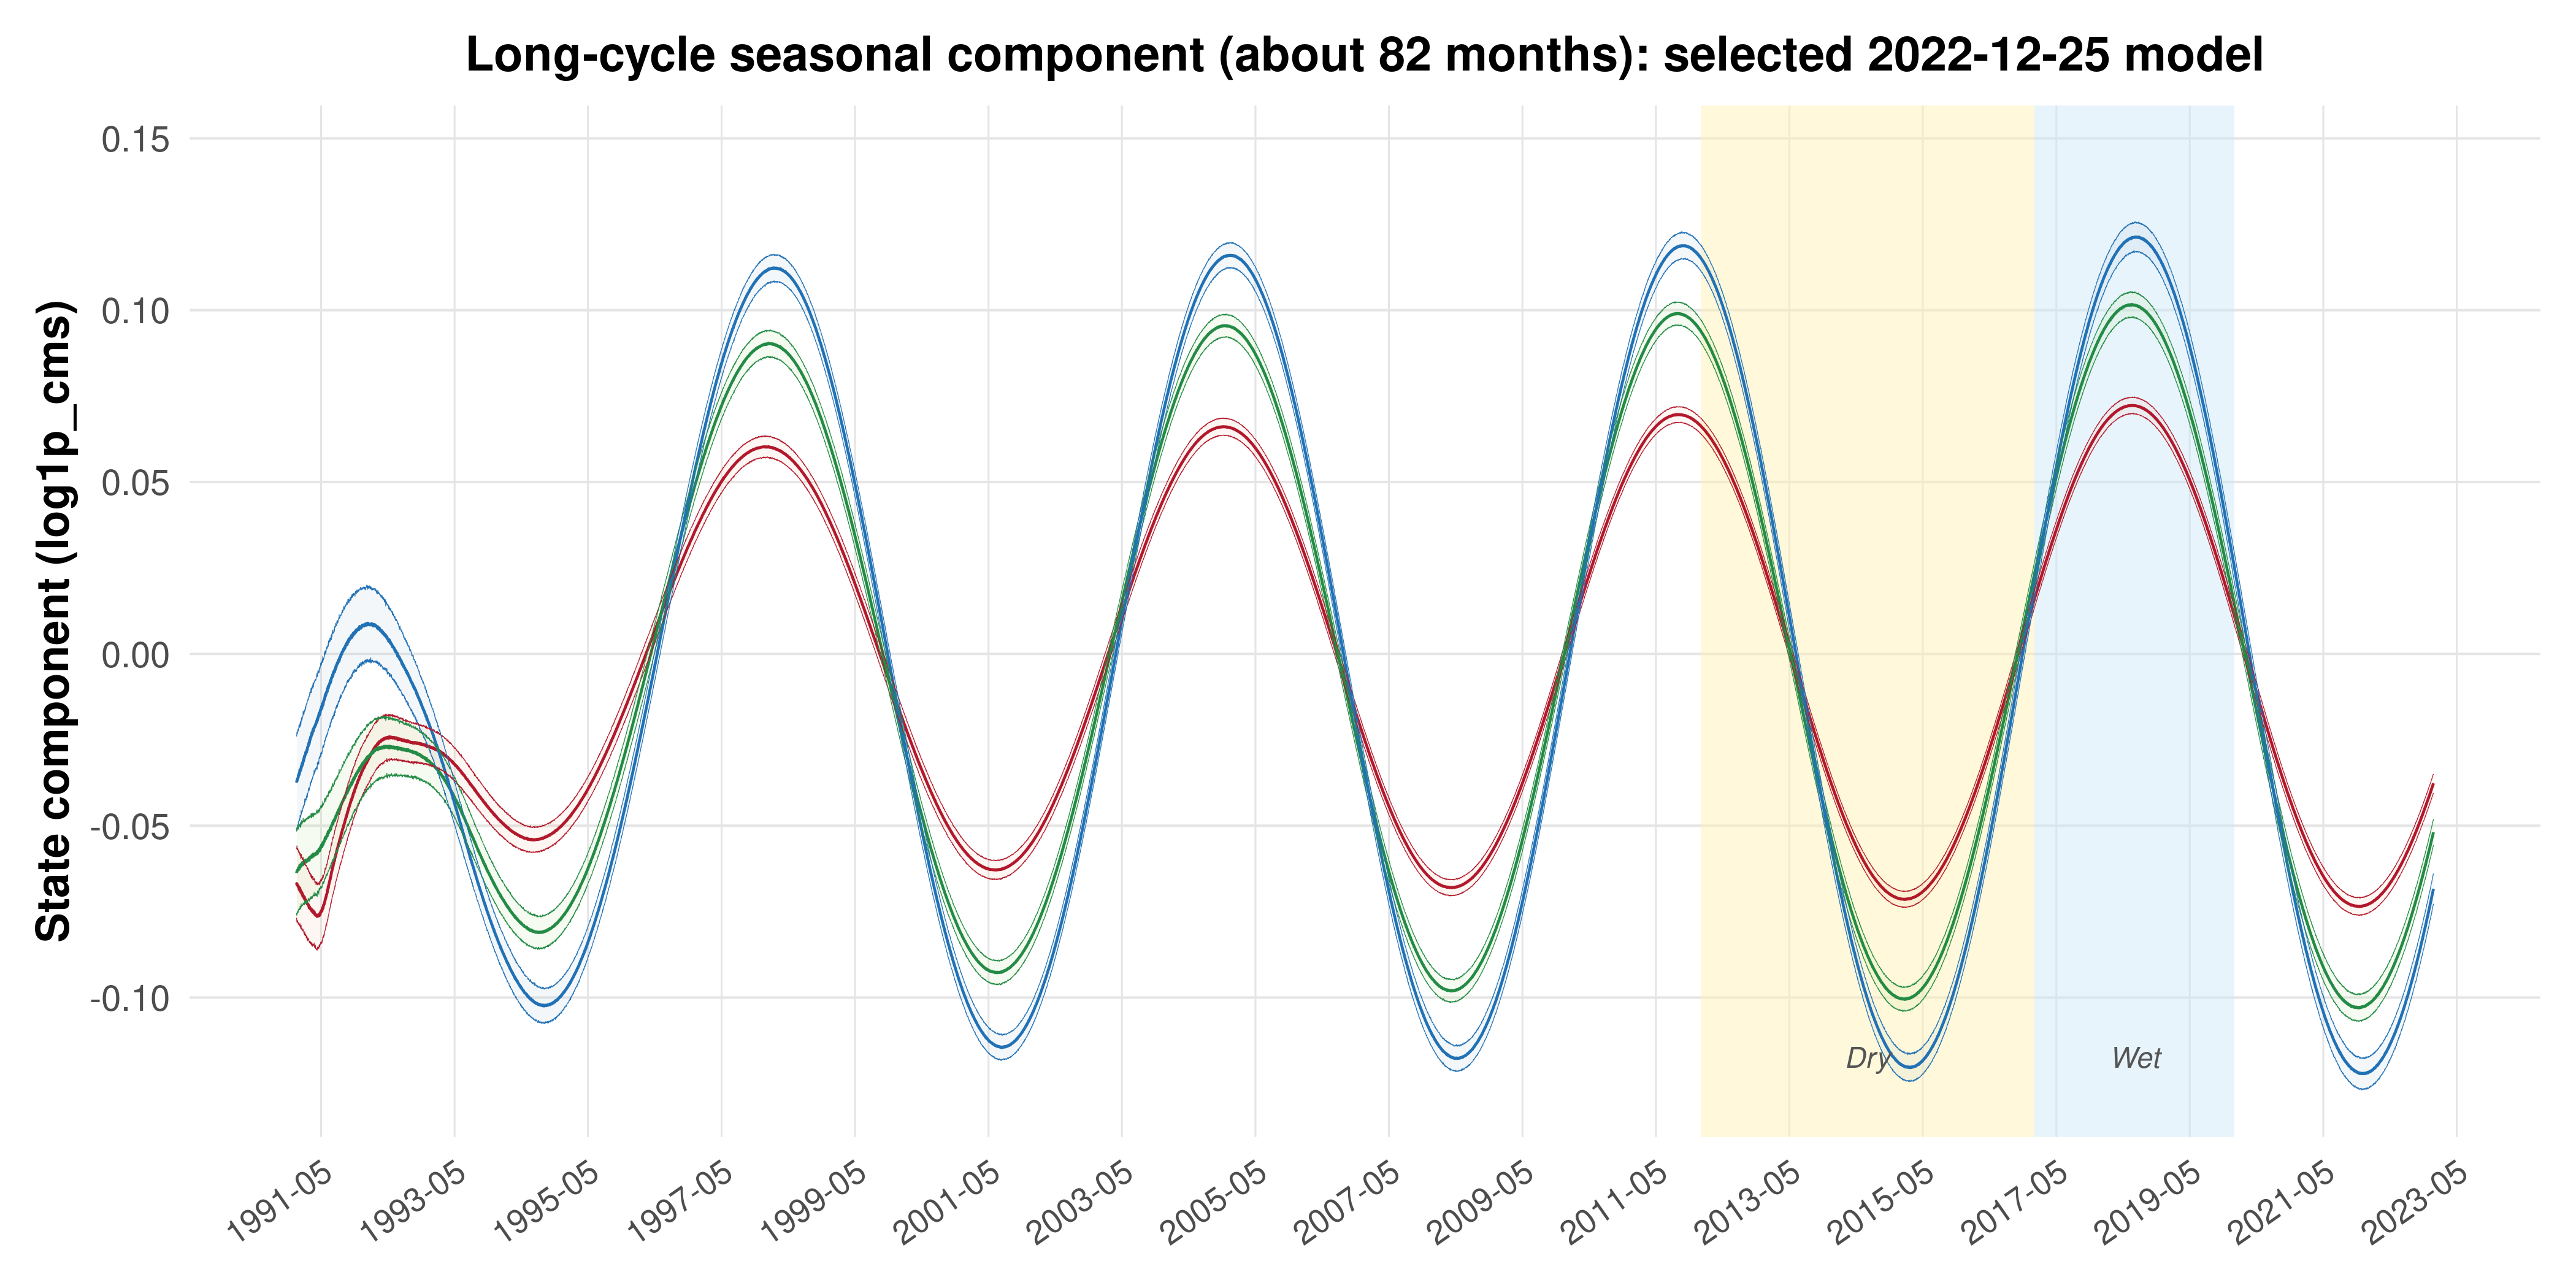
\includegraphics[width=\textwidth]{figures/ch03-environ/historical_component_80month.png}
\caption{
Selected-model posterior mean and 95\% credible intervals for the long-cycle seasonal component, with period approximately 6.81 years, or about 82 months, estimated from the 2022-12-25 cutoff exAL-M-T1 model. Estimates are shown for the 5th (red), 50th (green), and 95th (blue) quantiles. Shaded regions mark the 2012--2016 dry period and the 2017--2019 wet period.
}
\label{env:fig:80_components}
\end{figure}


\subsection{Predictive synthesis illustration}
\label{env:subsec:synthillustration}

The posterior bands in Figure~\ref{env:fig:dry_quantile} summarize uncertainty
around fitted quantile-location curves. Figure~\ref{env:fig:synth1} instead
shows the synthesized posterior predictive distribution for the December 25,
2022 cutoff, after combining the quantile-specific forecasts, source
corrections, and forecast-window inputs. It illustrates how the fitted
quantile-specific forecasts combine into one predictive distribution for a
given forecast origin.

\begin{figure}[htbp]
\centering
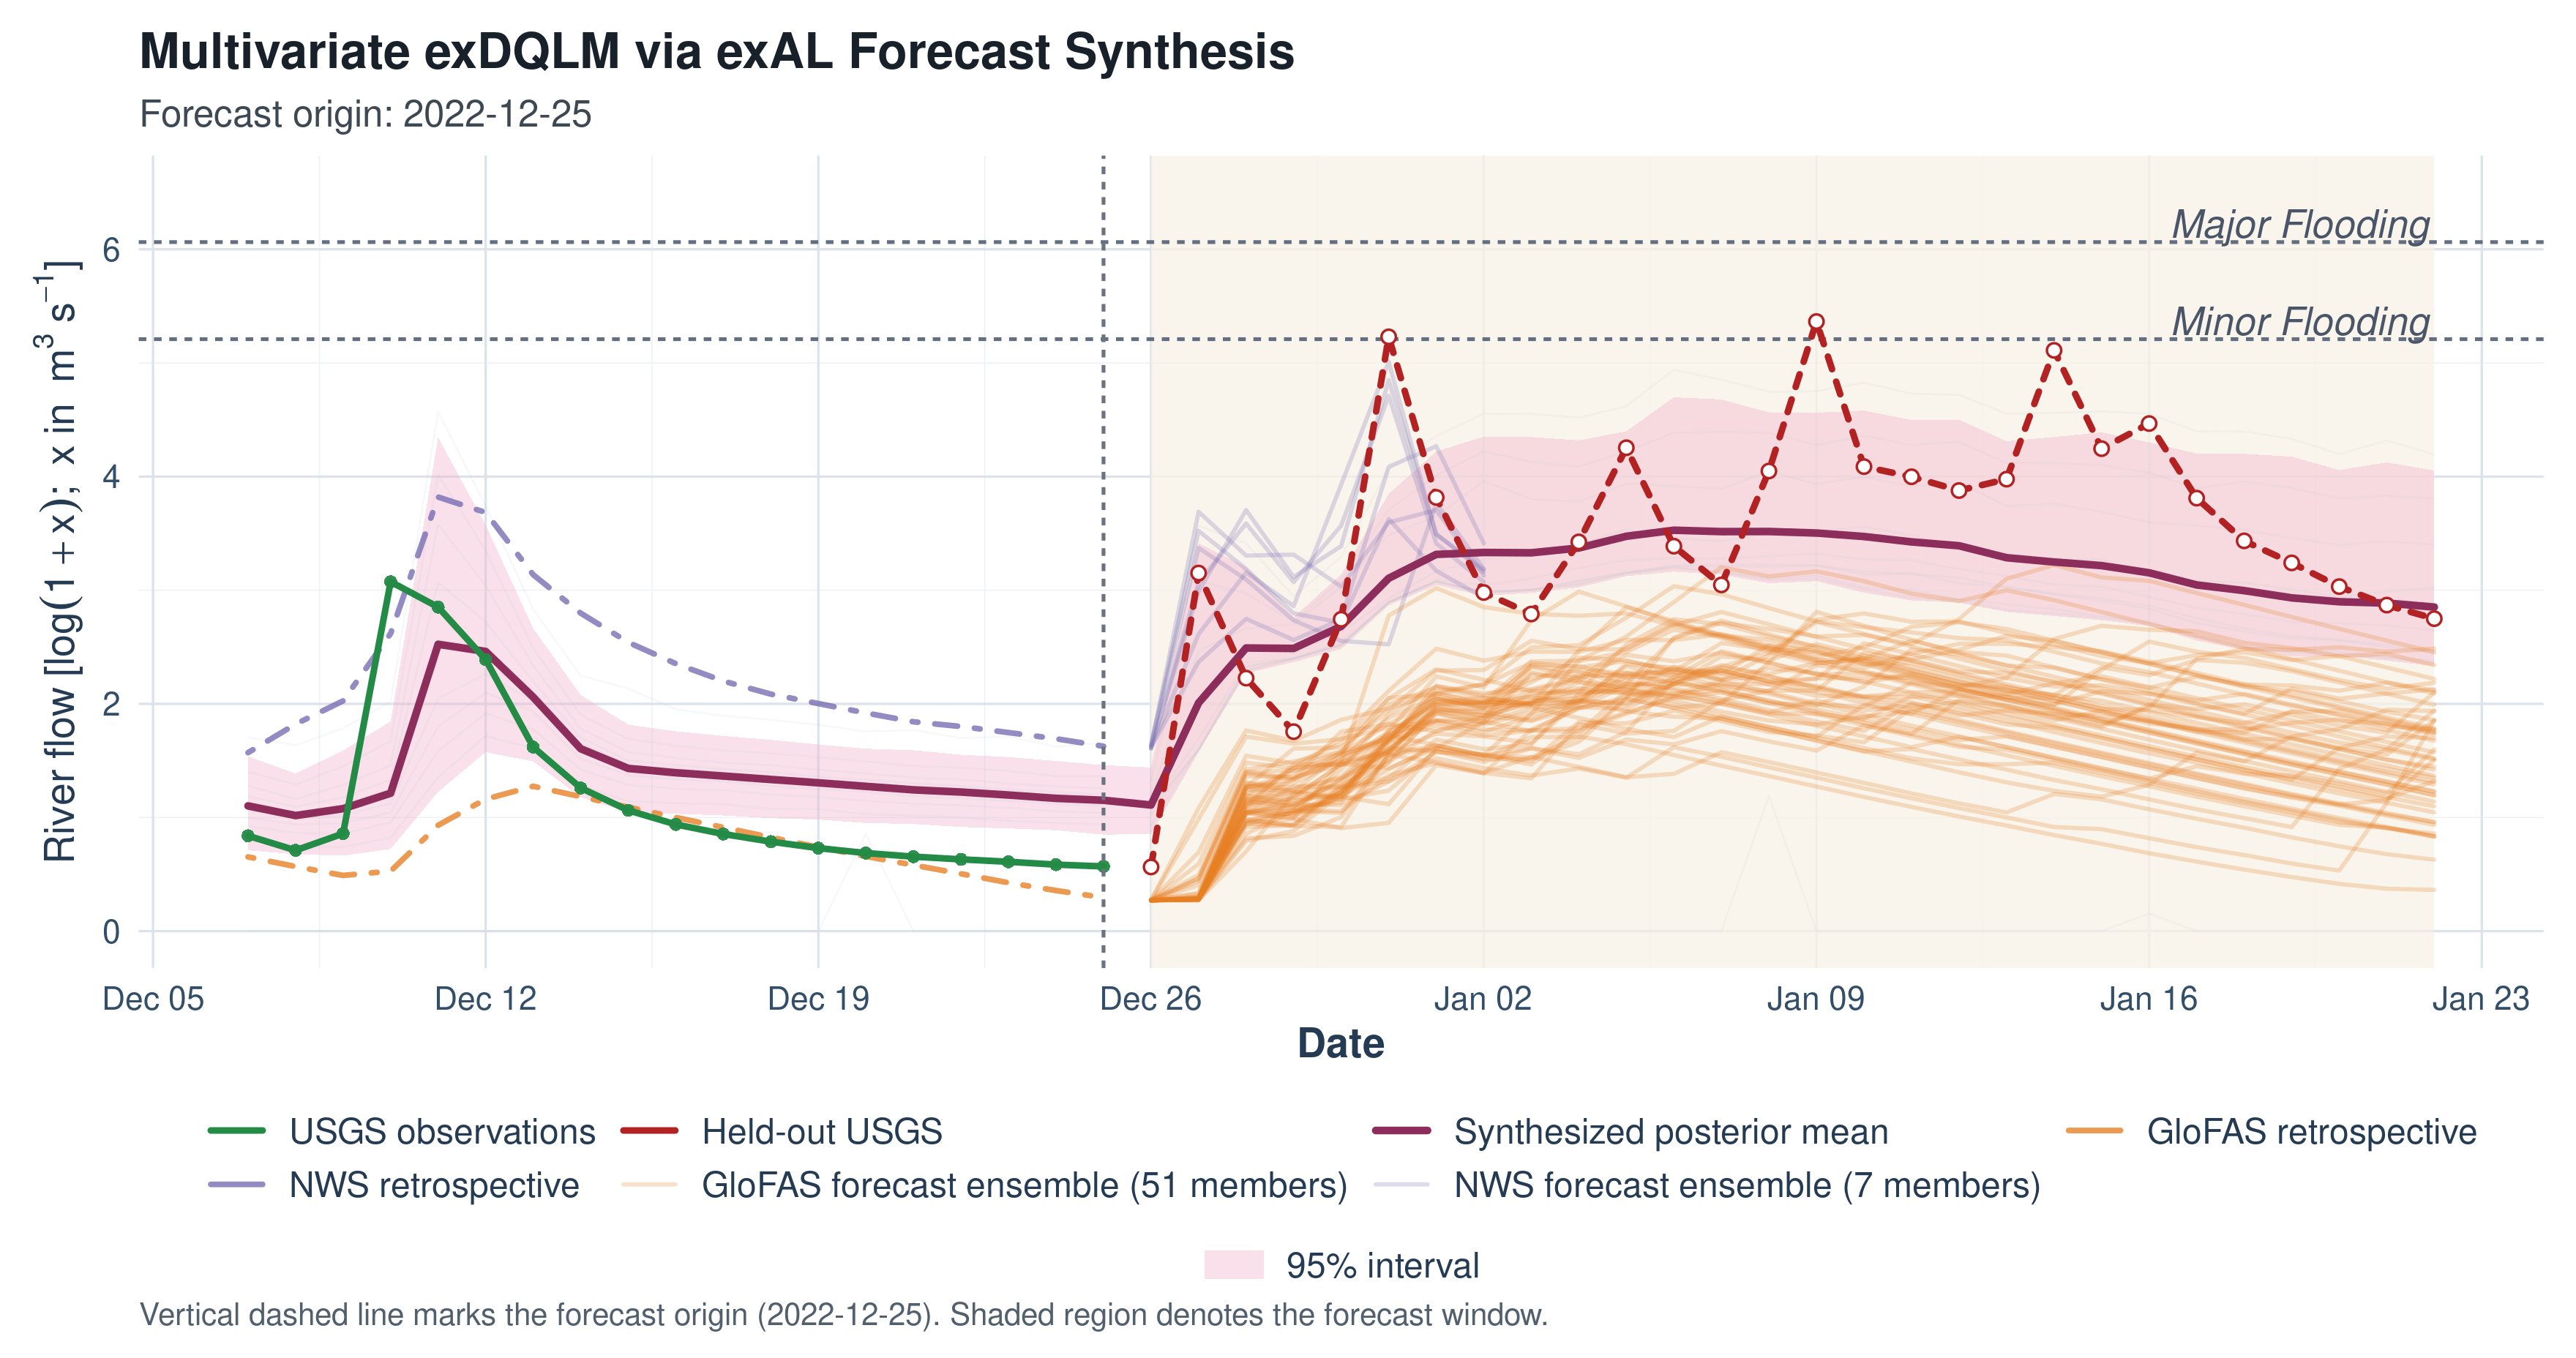
\includegraphics[width=\textwidth]{figures/ch03-environ/cutoff_2022_12_25_multivariate_synthesis_with_reference_ensembles.png}
\caption{
Synthesized posterior predictive distribution for river flow on the $\log(1+x)$ scale, with $x$ measured in m$^3$/s, at the December 25, 2022 forecast origin under the exAL-M-T1 model. Observed USGS measurements before the origin are shown in green, and held-out USGS verification after the origin is shown in red. The pink band is the central 95\% posterior predictive band from the synthesized distribution, and the dark center line summarizes the corresponding synthesized center. Thin overlaid lines correspond to displayed forecast quantiles at levels 0.05, 0.20, 0.35, 0.50, 0.65, 0.80, and 0.95. The raw retrospective and forecast products used at this cutoff are shown for context.
}
\label{env:fig:synth1}
\end{figure}
Because exAL-M-T1 is the selected extended-likelihood multivariate
specification, Figure~\ref{env:fig:synth1} is the main predictive-synthesis
illustration. The synthesized predictive distribution combines observed USGS
measurements before the cutoff with the retrospective and forecast products
available at that origin. The upper quantiles rise sharply after December 25,
2022 and reach levels comparable to the current-rating major-stage discharge
reference, reflecting the high-flow risk in this forecast window. Unlike the
fitted historical quantile-location summaries, the posterior predictive
envelope can vary across the forecast window as the source-specific corrections
and forecast-window covariates change. The corresponding univariate
transfer-active reference excludes both retrospective-product and forecast-
product source channels; it is retained as a secondary diagnostic, whereas the
multivariate display and the horizon-matched score tables provide
the claim-bearing evidence here. Figure~\ref{env:fig:synthsupport_20210123}
and Figure~\ref{env:fig:synthsupport_20211221} collect the other four
cutoff-specific multivariate panels in paired displays.

\subsection{Additional diagnostic evidence}
\label{environ:sec:body-additional-diagnostics}

Source-specific exAL summaries and cutoff-specific predictive-synthesis panels
support the interpretation above but are not required to follow the principal
five-origin comparison.  They are collected in
Appendix~\ref{app:hydrology-technical}, where their narrower diagnostic role
and the distinct evaluation horizons remain explicit.

\section{Chapter summary and limitations}
\label{env:sec5}

We developed a Bayesian quantile-based correction-and-synthesis framework for river-flow forecasting that links USGS observations, retrospective products, and forecast products through a shared latent quantile process. The framework combines source-specific discrepancy learning over the pre-cutoff observation window with a forecast-window synthesis step that propagates discrepancy corrections learned from retrospective products together with forecast-window transfer covariates. Variational Bayes based on Laplace--Delta approximations provides a lower-cost approximate alternative to full MCMC for fitting the extended dynamic quantile linear model.

In the San Lorenzo River application, the main empirical result is the five-cutoff rolling-origin forecast comparison based on the latest forecast products available at each cutoff. Relative to simpler Bayesian variants, the multivariate specifications with an active forecast-window transfer component provide the strongest performance in the 28-day synthesis comparison. The selected exAL-M-T1 specification attains the lowest 28-day forecast-window CRPS in all five cutoffs. A separate eight-day NWS-horizon table preserves the direct operational comparison to NWS without mixing forecast horizons. Taken together, the results support the value of source-aware multivariate correction for the 28-day forecast window, while the shorter NWS-horizon comparison shows that gains are not uniform across every origin and horizon.

The selected specification remains interpretable through its dynamic decomposition into source-specific corrections, trend, seasonal structure, and transfer effects. Its fitted transfer coefficients are quantile-specific rather than uniform: in the representative cutoff, local precipitation and soil moisture have negative coefficients in the lower and median quantile fits and positive coefficients in the 95th quantile fit, while the first GDPC coefficient is comparatively small on the reported scale. The regime diagnostics similarly separate fitted historical behavior into trend, seasonal, and transfer structure, with wider separation between lower and upper fitted quantiles during wetter, high-flow periods than during dry periods.

The framework still depends on the quality and compatibility of the external products and on the availability of forecast covariates at each forecast origin. The five-cutoff evaluation is not a dense continuous hindcast; the limiting step for such an extension is reconstructing version-consistent historical forecast-origin bundles, not only refitting the state-space models. In the present implementation, forecast-window GEFS precipitation and shallow soil-water ensembles enter through deterministic covariate summaries; future work could propagate the full uncertainty in these exogenous forecasts jointly with the river-flow synthesis. Natural extensions include joint treatment of multiple quantiles, richer dynamic structures for the discrepancy process, and spatial generalizations that couple nearby sites or basins.

\chapter{Bayesian quantile regression with deep echo state network features}
\label{ch:research-c}

\begin{singlespace}
\noindent\textit{This chapter is based on joint work by Antonio de Leon, Raquel Prado, and Bruno Sans\'o. It presents the current Q--DESN study; the posterior definitions, nonstandard computations, and claim-relevant sensitivity evidence are collected in Appendix~\ref{app:qdesn-technical}.}
\end{singlespace}

% Generated by scripts/refresh_current_research.py from the final values
% in the audited Q--DESN presentation-override chain.
\newcommand{\GlofasApplicationCurrentScoreTable}{tables/ch04-qdesn/glofas_forecast_correction_main_scores_display.tex}
\newcommand{\GlofasApplicationCurrentSupplementScoreTable}{tables/ch04-qdesn/glofas_reference_discrepancy_scores_display.tex}
\newcommand{\GlofasApplicationCurrentCalibrationTable}{tables/ch04-qdesn/glofas_empirical_quantile_frequencies_display.tex}
\newcommand{\GlofasApplicationCurrentConvergenceTable}{tables/ch04-qdesn/glofas_variational_stopping_display.tex}
\newcommand{\GlofasApplicationCurrentSpecificationsTable}{tables/ch04-qdesn/glofas_selected_specifications_display.tex}
\newcommand{\GlofasApplicationCurrentPriorSettingsTable}{tables/ch04-qdesn/glofas_issued_prior_settings_display.tex}
\newcommand{\GlofasApplicationCurrentPartOneTwoThreePriorSettingsTable}{tables/ch04-qdesn/glofas_reference_discrepancy_priors_display.tex}
\newcommand{\GlofasApplicationCurrentForecastWindowFigure}{figures/ch04-qdesn/glofas_application/glofas_common_window_statistical_labels_20261019.pdf}
\newcommand{\GlofasApplicationCurrentPartOneFigure}{figures/ch04-qdesn/glofas_application/glofas_editorial_20261013_reference.pdf}
\newcommand{\GlofasApplicationCurrentPartTwoFigure}{figures/ch04-qdesn/glofas_application/glofas_editorial_20261013_discrepancy.pdf}
\newcommand{\GlofasApplicationCurrentPartThreeFigure}{figures/ch04-qdesn/glofas_application/glofas_editorial_20261013_combined.pdf}
\newcommand{\GlofasApplicationCurrentConvergenceFigure}{figures/ch04-qdesn/glofas_application/glofas_editorial_20261013_convergence.pdf}
\newcommand{\GlofasApplicationCurrentCalibrationFigure}{figures/ch04-qdesn/glofas_application/glofas_editorial_20261013_calibration.pdf}
\newcommand{\GlofasApplicationCurrentQdesnAcrps}{0.7156}
\newcommand{\GlofasApplicationCurrentRawAcrps}{1.4360}
\newcommand{\GlofasApplicationCurrentScoredHorizons}{28}
\newcommand{\GlofasApplicationCurrentOriginDate}{2022-12-25}
\newcommand{\GlofasApplicationCurrentReferenceReservoirSize}{1500}
\newcommand{\GlofasApplicationCurrentReferenceReservoirMemory}{540}
\newcommand{\GlofasApplicationCurrentReferenceReservoirWashout}{500}
\newcommand{\GlofasApplicationCurrentReferenceReservoirAlpha}{0.75}
\newcommand{\GlofasApplicationCurrentReferenceReservoirRho}{0.6}
\newcommand{\GlofasApplicationCurrentReferenceReservoirSeed}{20260512}
\newcommand{\GlofasApplicationCurrentDiscrepancyReservoirSize}{1000}
\newcommand{\GlofasApplicationCurrentDiscrepancyReservoirMemory}{180}
\newcommand{\GlofasApplicationCurrentDiscrepancyReservoirWashout}{500}
\newcommand{\GlofasApplicationCurrentDiscrepancyReservoirAlpha}{0.85}
\newcommand{\GlofasApplicationCurrentDiscrepancyReservoirRho}{0.2}
\newcommand{\GlofasApplicationCurrentDiscrepancyReservoirSeed}{20261521}
\newcommand{\GlofasApplicationCurrentFullComparisonFigure}{figures/ch04-qdesn/glofas_application/glofas_editorial_20261013_issued.pdf}
\newcommand{\PricefmFullRegionFolds}{114}
\newcommand{\PricefmFullRegions}{38}
\newcommand{\PricefmFullFolds}{3}
\newcommand{\PricefmFullQdesnWins}{54}
\newcommand{\PricefmFullMeanQdesnAql}{7.217}
\newcommand{\PricefmFullMeanPricefmAql}{7.039}
\newcommand{\PricefmFullMeanDeltaAql}{+0.178}
\newcommand{\PricefmFullPaperQuantiles}{0.10, 0.25, 0.45, 0.50, 0.55, 0.75, 0.90}
\newcommand{\PricefmCurrentRegionFigure}{figures/ch04-qdesn/pricefm_application/pricefm_regional_aql_editorial_20261013_fontsafe.pdf}

% Restrained print palette and TikZ styles for the initialization diagram.
% Model families are identified by text and position in addition to color.
\definecolor{qiText}{HTML}{202124}
\definecolor{qiLine}{HTML}{62676C}
\definecolor{qiGaussian}{HTML}{737A80}
\definecolor{qiAL}{HTML}{31566D}
\definecolor{qiExAL}{HTML}{70444B}
\tikzset{
  qi/base/.style={rectangle,rounded corners=0pt,draw=qiLine,
    fill=white,text=qiText,line width=0.55pt,align=center,
    font=\normalfont\rmfamily\fontsize{9.5}{11}\selectfont,
    inner xsep=2.5pt,inner ysep=3pt,outer sep=0.3pt,
    minimum height=10mm},
  qi/gaussian/.style={qi/base,draw=qiGaussian},
  qi/al/.style={qi/base,draw=qiAL},
  qi/exal/.style={qi/base,draw=qiExAL},
  qi/heading/.style={text=qiText,align=left,inner sep=0pt,
    font=\normalfont\rmfamily\bfseries\fontsize{10}{11.5}\selectfont},
  qi/note/.style={text=qiText,align=left,inner sep=0pt,
    font=\normalfont\rmfamily\fontsize{9}{10.5}\selectfont},
  qi/dots/.style={inner sep=0.4pt,text=qiText,
    font=\normalfont\rmfamily\fontsize{9.5}{11}\selectfont},
  qi/arrow/.style={draw=qiLine,line width=0.55pt,
    -{Latex[length=1.65mm,width=1.12mm]},
    shorten <=0.35pt,shorten >=0.35pt},
  qi/collection/.style={draw=qiLine,line width=0.55pt},
  qi/comparison/.style={qi/arrow,dash pattern=on 2.5pt off 1.8pt}
}


\section{Introduction}
\label{qdesn2026:sec:intro}

Conditional quantiles describe tail risk and provide forecasts suited to
asymmetric decision losses and prediction intervals
\citep{qdesn-KoenkerBassett1978,qdesn-Koenker2005,qdesn-Gneiting2011}. Let \(Y_{t+h}\) be the
response \(h\) steps after forecast origin \(t\), and let \(\mathcal F_t\)
denote the information available at that origin. Its level-\(p\) conditional
quantile is
\[
\text{Forecast quantile:}\quad
Q_{t,h}(p)=\inf\{u:\Pr(Y_{t+h}\le u\mid\mathcal F_t)\ge p\},
\qquad 0<p<1.
\]
Conditional quantiles can depend nonlinearly on past responses and covariates.
Fitting Bayesian quantile models with many unknown recurrent-network weights
can be computationally demanding, particularly when separate models are
estimated at several quantile levels or refitted for rolling-origin validation.

We introduce the quantile deep echo state network (Q--DESN), a Bayesian
quantile regression model with nonlinear temporal predictors generated by a
specified deep echo state network (DESN). The network transforms response
history and covariates into recurrent predictors, with randomly drawn
reservoir weights held fixed before regression fitting. Conditional on these
predictors, the quantile location is linear in the coefficients of the final
regression layer (the readout), so the model retains a linear regression
structure while representing
nonlinear temporal dependence. We regularize the slopes with ridge or
regularized-horseshoe (RHS) priors and specify the intercept prior separately.
Ridge uses a common shrinkage scale, whereas RHS permits coefficient-specific
shrinkage and bounds conditional coefficient variances through a slab
\citep{qdesn-CarvalhoPolsonScott2010HS,qdesn-PiironenVehtari2017RHS}.
The multiquantile deep echo state network (MQ--DESN) extends this regression
across probability levels, estimating their readouts jointly under RHS priors
on adjacent slope differences.

The asymmetric Laplace (AL) likelihood links its location to a specified
conditional quantile and admits a normal--exponential augmentation
\citep{env-yu2001bayesian,qdesn-KozumiKobayashi2011Gibbs}. Under misspecification,
however, AL coefficient credible intervals need not have nominal frequentist
coverage \citep{qdesn-YangWangHe2016ALInference}. We also use the extended
asymmetric Laplace (exAL) likelihood, the quantile-fixed generalized
asymmetric Laplace family of \citet{exd-yan2025family}. Its additional shape
parameter allows skewness and tail behavior to vary while preserving the
quantile location. In their regression simulations, coefficient
credible-interval coverage was closer to nominal than under AL in
lower-tail settings.

For posterior simulation under AL, the augmentation gives standard full
conditional distributions for both Q--DESN and MQ--DESN regressions,
supporting efficient Gibbs-based Markov chain Monte Carlo (MCMC).
When repeated fitting makes posterior simulation costly, we also use
model-specific variational Bayes (VB) approximations, which can supply
starting values for MCMC under the corresponding model.

Echo state networks (ESNs) generate dynamic predictors from recurrent states
with fixed internal weights
\citep{qdesn-Jaeger2001EchoState,qdesn-LukoseviciusJaeger2009ReservoirComputing}.
Stacking reservoirs extends this construction to a DESN
\citep{qdesn-GallicchioMicheliPedrelli2018DeepESNDesign}. Bayesian regression on
reservoir features has precedent in the hierarchical Bayesian DESN of
\citet{qdesn-McDermottWikle2018DeepESNUQ}, developed for spatiotemporal forecasting.

Quantile reservoir methods also have precedent.
\citet{qdesn-LvZhaoLiuWang2016QRESNE} estimate ESN output weights by quantile
regression and combine quantile fits in a bootstrap ensemble for confidence
and prediction intervals. \citet{qdesn-BonasWikleCastruccio2024CalibratedDeepESN}
first fit DESN point forecasts by ridge regression, then jointly estimate
lead-dependent residual quantiles with penalized quantile sheets and
calibrate the resulting intervals. In contrast, Q--DESN estimates response
quantiles directly through Bayesian regression on DESN features, with
posterior inference for coefficients, likelihood parameters, and shrinkage
scales. For interval forecasts, it uses pairs of fitted response quantiles
without a second-stage residual-calibration regression or bootstrap ensemble.
MQ--DESN estimates the quantile readouts together
within one Bayesian regression, for which we derive MCMC updates and
model-specific VB approximations. Its conditional-quantile forecasts thus
follow directly from the fitted regression, rather than from estimating
residual quantiles after point prediction.

Independently estimated quantile curves can cross. Common post-estimation
corrections include monotone rearrangement, which reorders fitted quantiles,
and isotonic regression, which projects them onto an ordered grid
\citep{qdesn-BarlowBrunk1972IsotonicDual,exd-chernozhukov2010,qdesn-DeLeonPradoSanso2026HydrologicProducts}.
Alternatively, ordering can be imposed during estimation through noncrossing
constraints or a monotone quantile-process model
\citep{qdesn-WuLiu2009StepwiseNCQR,qdesn-BondellReichWang2010NoncrossingQR,qdesn-YangTokdar2017JointQuantilePlanes}.

MQ--DESN takes a continuous-shrinkage approach, adapting the
Quantile-Varying Parameter construction of \citet{qdesn-KohnsSzendrei2025QVP}.
RHS priors on adjacent slope differences favor similar neighboring slopes,
reducing predictor-dependent variation in the gaps between quantiles. With
ordered intercepts, this encourages nearly parallel, ordered quantile curves
while allowing quantile-specific effects. The resulting regularization
encourages noncrossing but does not enforce it.

Dynamic quantile linear models (DQLMs) and extended dynamic quantile linear
models (exDQLMs) represent temporal dependence through evolving linear states
\citep{env-goncalves,exd-me}.
\citet{qdesn-DeLeonPradoSanso2026HydrologicProducts} combine hydrologic products
through evolving linear quantile states and source-specific discrepancies,
fitting levels separately before predictive synthesis. Q--DESN instead
represents temporal dependence through recurrent nonlinear predictors, while
MQ--DESN couples coefficients across probability
levels. The first simulation examines whether Q--DESN can recover conditional
quantile paths and achieve forecast accuracy comparable to DQLMs and exDQLMs
under linear structural data-generating mechanisms.

The second simulation examines forecast scores and quantile ordering for
independent and joint estimation on a common seven-level grid. The
applications consider retrospective correction of streamflow ensemble
forecasts and electricity-price quantile forecasting against a pretrained
neural model. Sections~%
\ref{qdesn2026:sec:model}--%
\ref{qdesn2026:sec:forecast} define the model, computation, and forecast evaluation;
Sections~\ref{qdesn2026:sec:simulation}--\ref{qdesn2026:sec:pricefm-application} give the
evidence. Posterior derivations and supporting results are in
Appendices~\ref{app:qdesn-posterior}--\ref{app:qdesn-simulation-support}.

% ============================================================

\section{Fixed-feature Bayesian quantile models}
\label{qdesn2026:sec:model}

\subsection{Single-level quantile regression}

Let \(Y_t\), \(t=1,\ldots,T\), be the response, with observed value
\(y_t\), and let
\(\vect x_t=(1,\tilde{\vect x}_t^\top)^\top\in\R^{r+1}\) be a specified
vector containing an intercept and \(r\) temporal predictors. Write
\(\vect\beta=(\beta_0,\vect\beta_{\mathrm{slope}}^\top)^\top\in\R^{r+1}\).
At probability level \(p_0\in(0,1)\), the linear quantile regression is
\begin{equation}
\begin{aligned}
\text{Quantile location:}\quad &\mu_t=\vect x_t^\top\vect\beta,\\
\text{Likelihood:}\quad
&Y_t\mid\vect x_t,\vect\beta,\sigma,\gamma
  \sim\exAL_{p_0}(\mu_t,\sigma,\gamma),\qquad t=1,\ldots,T.
\end{aligned}
\label{qdesn2026:eq:qdesn-marginal-main}
\end{equation}
Under this likelihood, \(\mu_t\) is the conditional \(p_0\)-quantile,
\(\sigma>0\) controls scale, and \(\gamma\in(L,U)\) controls shape. The
shape interval \((L,U)\) is determined by \(p_0\). Setting \(\gamma=0\)
recovers the AL regression. Section~\ref{qdesn2026:subsec:desn-features} constructs
\(\vect x_t\) from the response
history and covariates. Conditional on that design, the location in
Eq.~\eqref{qdesn2026:eq:qdesn-marginal-main} is linear in \(\vect\beta\).

\subsection{Deep echo state network features}
\label{qdesn2026:subsec:desn-features}

Let \(\vect z_t\in\R^q\) contain the exogenous variables and let
\(\vect u_t=(y_{t-1},\ldots,y_{t-m},\vect z_t^\top)^\top\in\R^{m+q}\)
contain these variables with \(m\) response lags. In a network with \(D\)
layers, the reservoir state
\(\vect h_{t,d}\in\R^{n_d}\) is a recurrent nonlinear transformation of
these inputs. For layer \(d\), \(\bar{\mat W}_d\) is a fixed sparse recurrent
matrix scaled to spectral radius \(\rho_d\), its largest absolute eigenvalue;
\(\mat W_d^{\mathrm{in}}\) is a fixed input matrix, and \(\alpha_d\) is the
leak rate. Between layers, the dimension-reduction matrix \(\mat Q_{d-1}\) gives
\(\tilde{\vect h}_{t,d-1}=\mat Q_{d-1}\vect h_{t,d-1}\).
The nonlinear activation function \(f\) acts componentwise, and \(k\) is a chosen feature
transformation.
With a fixed first-layer input bias \(\vect b_1^{\mathrm{in}}\), the
recursion and general feature vector are
\begingroup\scriptsize\begin{equation}
\begin{alignedat}{2}
\text{First layer:}\quad &\vect h_{t,1}
&&=(1-\alpha_1)\vect h_{t-1,1}\\
&&&\quad+\alpha_1 f(\bar{\mat W}_1\vect h_{t-1,1}
+\mat W_1^{\mathrm{in}}\vect u_t+\vect b_1^{\mathrm{in}}),\\
\text{Higher layers:}\quad &\vect h_{t,d}
&&=(1-\alpha_d)\vect h_{t-1,d}\\
&&&\quad+\alpha_d f(\bar{\mat W}_d\vect h_{t-1,d}
+\mat W_d^{\mathrm{in}}\tilde{\vect h}_{t,d-1}),\quad d=2,\ldots,D,\\
\text{Features:}\quad &\tilde{\vect x}_t
&&=\big[\vect h_{t,D}^\top,k(\tilde{\vect h}_{t,1})^\top,\ldots,
k(\tilde{\vect h}_{t,D-1})^\top,\vect u_t^\top\big]^\top.
\end{alignedat}
\label{qdesn2026:eq:desn-hierarchy}
\end{equation}\endgroup
The fixed matrix \(\mat Q_d\) maps \(\R^{n_d}\) to \(\R^{\tilde n_d}\).
Here \(\bar{\mat W}_d\) is \(n_d\times n_d\),
\(\mat W_1^{\mathrm{in}}\) is \(n_1\times(m+q)\), and
\(\mat W_d^{\mathrm{in}}\) is \(n_d\times\tilde n_{d-1}\) for \(d>1\).
A small leak rate retains more of the previous state. If \(k\) preserves
dimension, the displayed feature vector
has dimension \(r=n_D+\sum_{d<D}\tilde n_d+m+q\); a dimension-expanding
transformation changes this count. Appending the intercept gives \(\vect x_t\).
Reservoir and input weights are randomly drawn before fitting and then held
fixed. Scaling, dimension reduction, and the washout period used to discard initial
transients are determined from fitting information and held fixed.

The predictors used in each simulation or application are chosen reservoir
layers, transformations of their states, and direct inputs where included.
Appendix~\ref{app:qdesn-simulation-support} summarizes the selection criteria
and reservoir diagnostics. For observed fitting inputs, the resulting design matrix
\(\mat X=(\vect x_1,\ldots,\vect x_T)^\top\) is fixed. Future rows follow
the forecasting rule in Section~\ref{qdesn2026:sec:forecast}.

\subsection{Coefficient regularization}

The intercept has a separately specified Gaussian prior on the response scale
and is excluded from slope shrinkage. Intercept calibration and any ordering
restrictions for multiquantile fits are stated with each study. For the \(r\)
non-intercept
coefficients, ridge regularization uses
\(\vect\beta_{\mathrm{slope}}\sim
\Normal(\zeros{r},\kappa_\beta^2\Id{r})\), with common prior standard
deviation \(\kappa_\beta\). The adaptive alternative uses the
Nishimura--Suchard product form of the regularized horseshoe
\citep{qdesn-MakalicSchmidt2016SimpleSampler,exd-nishimura2023shrunken}. For the
\(j\)th slope \(\beta_j\), conditional on global, local, and slab scales
\((\tau,\lambda_j,\zeta)\),
\begin{equation}
\begin{aligned}
\text{Slope prior:}\quad
&\beta_j\mid\tau,\lambda_j,\zeta\sim\Normal(0,V_j),\\
\text{Effective variance:}\quad
&V_j=\left(\zeta^{-2}+\tau^{-2}\lambda_j^{-2}\right)^{-1},
\qquad j=1,\ldots,r.
\end{aligned}
\label{qdesn2026:eq:rhs-var}
\end{equation}
The local and global scale factors use the half-Cauchy auxiliary hierarchy,
with reference scales one and \(\tau_0\), respectively; \(\zeta^2\) bounds the
coefficient variances in Eq.~\eqref{qdesn2026:eq:rhs-var}. The complete product hierarchy
and slab treatment are given in Appendix~\ref{app:qdesn-posterior}.

The fixed hyperprior scale \(\tau_0\) controls prior shrinkage through the
random global scale \(\tau\). For standardized predictors, a Gaussian
regression calculation provides a reference for \(\tau_0\) from a residual standard
deviation, fitting-sample size, and a prior reference number of coefficients
expected to escape strong shrinkage \citep{qdesn-PiironenVehtari2017RHS}; the
calibration principle and study-specific choices are recorded in
Appendix~\ref{app:qdesn-posterior}.

\subsection{Multiquantile regression (MQ--DESN)}
\label{qdesn2026:subsec:joint-qdesn}

Independent fits at \(K\) ordered levels \(0<p_1<\cdots<p_K<1\) assign a
separate quantile regression to each level. MQ--DESN instead uses
level-specific intercepts \(\beta_{0k}\) and slope vectors
\(\vect\beta_k\in\R^r\) on the same feature design:
\begin{equation}
\text{Quantile location:}\quad
\mu_{k,t}=\beta_{0k}+\tilde{\vect x}_t^\top\vect\beta_k,
\qquad k=1,\ldots,K.
\label{qdesn2026:eq:joint-qdesn-readout}
\end{equation}
Let \(\vect y=(y_1,\ldots,y_T)^\top\) be the observed response vector,
\(\theta\) collect the regression, likelihood, and prior-scale parameters,
and \(\pi(\theta)\) denote their prior. Write \(f_{p_k}\) for the AL or exAL
density at level \(p_k\), with scale \(\sigma_k\) and, for exAL, shape
\(\gamma_k\). The composite update is
\begin{equation}
\begin{aligned}
\text{Composite likelihood:}\quad
&L_c(\theta;\vect y,\mat X)
 =\prod_{t=1}^T\prod_{k=1}^K
 f_{p_k}(y_t\mid\mu_{k,t},\sigma_k,\gamma_k),\\
\text{Composite posterior:}\quad
&\pi_c(\theta\mid\vect y,\mat X)
 \propto\exp\!\left\{-\ell_c(\theta;\vect y,\mat X)\right\}\pi(\theta).
\end{aligned}
\label{qdesn2026:eq:joint-composite-posterior-main}
\end{equation}
Here \(\ell_c(\theta;\vect y,\mat X)=-\log L_c(\theta;\vect y,\mat X)\)
is the negative composite log-likelihood. The posterior is defined when its
normalizing constant is finite.
Each factor is a normalized density, but their product reuses the same
response across levels and is not a normalized scalar-response sampling
density. The prior couples levels by regularizing the first slope vector
and adjacent differences,
\[
\text{Anchor and differences:}\quad
\vect\Delta_1=\vect\beta_1,\qquad
\vect\Delta_k=\vect\beta_k-\vect\beta_{k-1},\quad k=2,\ldots,K.
\]
Each block uses RHS shrinkage with block-specific global and local scales.
When \(K=1\), the hierarchy
recovers the single-level Q--DESN slope prior under RHS regularization.

Adjacent-difference shrinkage favors similar neighboring slopes but does not
ensure noncrossing: the adjacent location gap
\[
\text{Adjacent location gap:}\quad
\mu_{k,t}-\mu_{k-1,t}
=(\beta_{0k}-\beta_{0,k-1})
+\tilde{\vect x}_t^\top(\vect\beta_k-\vect\beta_{k-1})
\]
can be negative. Appendix~\ref{app:qdesn-posterior} gives
the fitted hierarchy and its precision matrix, while
Appendix~\ref{app:qdesn-computation} records the intercept-order
restrictions used in each analysis.

% ============================================================

\section{Posterior computation}
\label{qdesn2026:sec:inference}

Conditional on the design, the posterior combines the likelihood in
Eq.~\eqref{qdesn2026:eq:qdesn-marginal-main} with the coefficient, scale, and shape
priors. MQ--DESN uses the composite posterior in
Eq.~\eqref{qdesn2026:eq:joint-composite-posterior-main} and the adjacent-difference
hierarchy. For computation, exAL admits the equivalent
augmentation
\begingroup\scriptsize\begin{equation}
\begin{alignedat}{2}
\text{Latent variables:}\quad
&v_t\mid\sigma&&\sim\Exp(\mathrm{rate}=1/\sigma),
\qquad s_t\sim\TN(0,1),\\
\text{Gaussian conditional:}\quad
&Y_t\mid\cdot&&\sim\Normal\!\left(
\vect x_t^\top\vect\beta+D_{p_0}(\gamma)\sigma s_t
+A_{p_0}(\gamma)v_t,
B_{p_0}(\gamma)\sigma v_t\right).
\end{alignedat}
\label{qdesn2026:eq:qdesn-aug}
\end{equation}\endgroup
Appendix~\ref{app:qdesn-posterior} defines the
probability-specific functions \(A_{p_0}\), \(B_{p_0}\), and \(D_{p_0}\);
\(D_{p_0}\) is the latent-shift coefficient. Here \(\TN(0,1)\) denotes a
standard Normal distribution truncated to \((0,\infty)\), and the second
Gaussian argument is a variance.
Integrating out \((s_t,v_t)\) recovers the marginal exAL model. For AL,
shape is fixed at zero and the latent shift term is absent.

Conditional on latent variables and prior scales, unconstrained coefficient
blocks have Gaussian updates; ordered intercepts use Gaussian conditionals
truncated between neighboring intercepts. Under the product RHS hierarchy,
squared local and global scales, their auxiliaries, and any random squared
slab scale have inverse-gamma updates. AL mixture
variables have generalized inverse-Gaussian updates, and its likelihood scale
has an inverse-gamma update. Under exAL, the mixture variables still have
generalized inverse-Gaussian updates, while the additional \(s_t\) variables
have positive truncated-normal updates.
Conditional on shape, its scale has a generalized inverse-Gaussian law, but
the joint scale--shape block remains nonconjugate. The exAL simulation MCMC
transitions integrate scale out of the shape update and then redraw it from
its conditional law. Convergence assessment includes rank-normalized
\(\widehat R\), effective sample sizes, chain comparisons of reported
scores and forecast summaries, and quantile-crossing diagnostics.

Variational Bayes approximates the posterior through model-specific factors
and supports fast repeated fitting. Completed variational fits can supply
starting values for MCMC under the corresponding model. Appendix~\ref{app:qdesn-computation}
gives the factors and updates, including the Laplace--Delta approximation
of \citet{exd-wang2013nonconjugatevb} and the structured scale--shape
approximation used in the multiquantile simulation.

% ============================================================

\section{Forecasting, scoring, and model selection}
\label{qdesn2026:sec:forecast}

\subsection{Multi-step quantile forecasts}

A forecast origin \(o\) is the last time included in its observed history
and may differ from the fitting endpoint \(T\); horizon \(h\) denotes
prediction of \(Y_{o+h}\). Reservoir states are reconstructed
from that history. Within each recursive forecast, unknown responses are
generated under the stated response law, and their lags enter subsequent
updates. At a fitted probability level \(p\), posterior or variational draw
\(b\) and its simulated path yield the conditional-quantile location
\(\mu_{o+h,p}^{(b)}=\beta_{0p}^{(b)}
+\tilde{\vect x}_{o+h}^{(b)\top}\vect\beta_p^{(b)}\).
A marginal posterior predictive quantile instead integrates the response
distribution over parameter and future-path uncertainty before taking its
quantile. Appendix~\ref{app:qdesn-simulation-support} specifies the response laws
used to generate future lags.

\subsection{Forecast scores}

Write \(\vect q^*=(q_1^*,\ldots,q_K^*)^\top\) for the quantile forecasts at
evaluation levels \(p_1,\ldots,p_K\), including any monotone adjustment
specified for the analysis. In the multiquantile simulation, equal-weight
isotonic projection orders each estimated grid to
address crossings; the projection and scoring range are defined in
Appendix~\ref{app:qdesn-simulation-support}.

For a quantile forecast \(q\) at level \(p\), let \(e=y-q\) be the forecast
error and define the check loss by
\begin{equation}
\text{Check loss:}\quad \rho_p(e)=e\{p-\ind(e<0)\}.
\label{qdesn2026:eq:check-loss-main}
\end{equation}
Here \(\ind(e<0)\) is the indicator of a negative error. For a predictive
distribution \(F\) with finite first moment and quantile function \(F^{-1}\),
the continuous ranked probability score (CRPS) has the integrated check-loss
representation
\citep{exd-gneiting2007}
\begin{equation}
\text{CRPS:}\quad \operatorname{CRPS}(F,y)
=2\int_0^1\rho_p\{y-F^{-1}(p)\}\,dp.
\label{qdesn2026:eq:crps-integrated-check-main}
\end{equation}
For \(0<p_1<\cdots<p_K<1\) and \(K\geq2\), the finite-grid approximate
CRPS (\(\aCRPS\)) applies the trapezoidal rule to
Eq.~\eqref{qdesn2026:eq:crps-integrated-check-main} over \([p_1,p_K]\),
\begin{equation}
\begin{aligned}
\text{Finite-grid score:}\quad
&\aCRPS_{p_1:p_K}(y;\vect q^*)
 =2\sum_{k=1}^K\omega_k\rho_{p_k}(y-q_k^*),\\
\text{Trapezoidal weights:}\quad
&\omega_1=\frac{p_2-p_1}{2},\\
&\omega_k=\frac{p_{k+1}-p_{k-1}}{2},\quad 2\leq k\leq K-1,\\
&\omega_K=\frac{p_K-p_{K-1}}{2}.
\end{aligned}
\label{qdesn2026:eq:acrps-main}
\end{equation}
The weights satisfy
\(\sum_{k=1}^K\omega_k=p_K-p_1\). Thus \(\aCRPS\) retains the scale of integrated
check loss over the evaluation range rather than representing a full-distribution
CRPS. The evaluation grid is common to the competing methods within each
analysis, not necessarily across analyses.

In the multiquantile simulation, the conditional data-generating process
(DGP) is known. Let
\(\mathcal E=\{(o_\ell,h_\ell):\ell=1,\ldots,N_{\mathrm{eval}}\}\)
be the \(N_{\mathrm{eval}}\) held-out origin--horizon pairs, and let
\(F_{0,\ell}(y)=\Pr_0(Y_{o_\ell+h_\ell}\le y
\mid\mathcal F_{o_\ell}^{\mathrm{obs}})\)
be the conditional DGP distribution given observed origin history
\(\mathcal F_{o_\ell}^{\mathrm{obs}}\), where \(\Pr_0\) denotes probability
under the DGP. For posterior draw \(b\), let \(q_{\ell,k}^{*,(b)}\) be the
adjusted quantile forecast at level \(p_k\) for pair \(\ell\); the oracle
finite-grid \(\aCRPS\) is
\begin{equation}
\text{Oracle score:}\quad S_{\mathrm{DGP}}^{(b)}
=\frac{2}{N_{\mathrm{eval}}}\sum_{\ell=1}^{N_{\mathrm{eval}}}
\sum_{k=1}^K\omega_k
\int\rho_{p_k}\!\left(y-q_{\ell,k}^{*,(b)}\right)\,dF_{0,\ell}(y).
\label{qdesn2026:eq:dgp-integrated-score-main}
\end{equation}
Here ``oracle'' refers to evaluating expected check loss under the known DGP.
Common simulated DGP paths approximate the expectations over future
responses. For the primary calculation, each model's future predictors are
averaged over simulated response paths before posterior coefficient draws
are evaluated. Score intervals condition on these averaged predictors.
Appendix~\ref{app:qdesn-simulation-support} reports the draw-specific
recursive-forecast sensitivity.

\subsection{DESN specification and selection}
\label{qdesn2026:sec:selection}

Candidate DESN specifications vary properties such as depth, layer size,
leak rate, input scaling, and reservoir realization. They are compared using
the observations and criterion specified for each study. Gaussian regressions
on DESN features (Gaussian-DESN) estimate the
conditional mean and provide an inexpensive first comparison through ridge
regularization; where used, Gaussian RHS--VB and quantile
regressions refine the comparison among promising specifications. For a
reference regression \(M\), candidate specifications \(R_1,\ldots,R_J\),
and a selection criterion \(S_{\mathrm{sel}}(R_j;M)\), selection takes
the form
\begin{equation}
\text{Selected reservoir:}\quad \widehat R_M
\in\argmin_{R_j:\,j=1,\ldots,J}
S_{\mathrm{sel}}(R_j;M).
\label{qdesn2026:eq:reservoir-selection-main}
\end{equation}
The selected DESN specification is held fixed for the reported posterior
summaries. In the
multiquantile simulation, the Gaussian-DESN comparison and subsequent refinement select
one specification for each mechanism. Its reservoir realization and feature
construction are shared by independent Q--DESN under AL and exAL and
MQ--DESN under AL and exAL. These four regressions
use the same selected temporal representation while differing in likelihood
and sharing across quantile levels. The single-quantile study uses a separate,
criterion-specific selection procedure.

Checks of the reservoir states assess finite values and saturation near the
limits of bounded activation functions. Checks of the resulting
predictors assess near-constant or highly dependent columns, effective rank,
conditioning, and variation across reservoir realizations. Together these
assess reservoir behavior under the observed inputs and the regression design, complementing the
study of leaky dynamics and the echo state property: the decay of initial-state
effects under a common input history
\citep{qdesn-JaegerLukoseviciusPopoviciSiewert2007LeakyESN,qdesn-YildizJaegerKiebel2012ESP}.


% ============================================================

\section{Simulation studies}
\label{qdesn2026:sec:simulation}

\noindent
Two studies examine forecast accuracy and recovery of known conditional
quantile paths. The first follows the error-family comparisons of
\citet{exd-yan2025family}, with a dynamic rather than static quantile path, and
compares single-level Q--DESN with dynamic linear baselines. The second
compares independent Q--DESN and MQ--DESN regressions using the same selected
DESN specification and reservoir realization. We use \(p\) for a single level and \(p_k\), \(k=1,\ldots,K\),
for a grid. Main-text figures report the primary MCMC forecast summaries;
Appendix~\ref{app:qdesn-simulation-support} retains the longer-window,
calibration, and recursive-path sensitivities needed to qualify them.

\subsection{Single-quantile simulation design}

The first study asks whether Q--DESN can recover quantile dynamics generated
by a linear trend and seasonal state model. Observation errors follow
Gaussian, Laplace, or Gaussian-mixture distributions. For each family \(f\), we
consider \(p\in\{0.05,0.25,0.50\}\) and shift the errors so that their
\(p\)-quantile is zero. The observation and state equations are
\begin{equation}
\begin{aligned}
\text{State evolution:}\quad
&\vect\theta_{t,f}=\mat G_\theta\vect\theta_{t-1,f}+\vect\eta_{t,f},
\quad \vect\eta_{t,f}\sim\Normal(\zeros{6},\mat W_\theta),\\
\text{Observation:}\quad
&y_{t,p,f}=\vect F^\top\vect\theta_{t,f}+e_{t,f}-H_f^{-1}(p),\\
\text{Conditional quantile:}\quad
&Q_p(Y_{t,p,f}\mid\vect\theta_{t,f})=\vect F^\top\vect\theta_{t,f}.
\end{aligned}
\label{qdesn2026:eq:single-quantile-dgp-main}
\end{equation}
Here \(H_f\) is the distribution function of the unshifted observation error,
and \(\vect F\) selects the level and seasonal components of the state.
The evolution matrix \(\mat G_\theta\) propagates a local linear trend and
seasonal harmonics, following the construction of \citet{exd-west1997bayesian};
\(\mat W_\theta\) controls their random changes over time. Within each
family, the latent quantile path is shared across the three levels, with only
the error-centering constant changing. Appendix~\ref{app:qdesn-simulation-support}
records the family-specific generating distributions and initial states.

Each model is fitted to 500 observations. The primary evaluation uses the
following 300 observations, giving ten origins and 300 scored origin--horizon
pairs. Forecasts are issued every 30 observations for horizons of up to
30 steps. A sensitivity analysis extends evaluation to the first 500
observations, with the last forecast truncated at that boundary. This shorter
primary period was adopted after exploratory assessment of the longer series;
the comparison is therefore development-informed rather than an untouched
confirmatory validation. All methods use the same pairs within each evaluation. Parameters are not
refitted between origins; newly available responses update the states or
recurrent features used for forecasting. The 300 origin--horizon pairs within
a family and quantile level come from one simulated trajectory, not 300
independent simulation replications. Posterior score intervals are therefore
conditional summaries for that trajectory and fitted model.

We compare Q--DESN under AL and exAL likelihoods, both with RHS coefficient
regularization, with DQLM and exDQLM fitted using \pkg{exdqlm}
\citep{env-deleon2026exdqlm}. The dynamic linear baselines use the generating
trend and seasonal structure. This provides a favorable structural benchmark
for assessing whether Q--DESN can represent linear temporal dependence
through recurrent features rather than an explicitly specified state
transition. Separate DESN specifications were selected for the reported
criteria; historical refinement also used forecast performance on the
evaluation series. Appendix~\ref{app:qdesn-simulation-support} describes this selection.
Consequently, the score comparisons characterize the frozen, selected
specifications on these simulated series; they are exploratory evidence rather
than performance on an untouched confirmation set.

Check loss evaluates the quantile forecasts against realized responses over
the common forecast pairs. The main comparison summarizes its posterior
distribution. Additional results assess recovery of the known
state-conditional quantile path using mean absolute error (MAE), together
with empirical quantile frequencies and fitting-sample recovery.

\subsection{Single-quantile results}

Figure~\ref{qdesn2026:fig:simulation-500obs-mcmc-forecast-check-loss-intervals}
summarizes posterior distributions of average forecast check loss.

At the lower quartile and median, both Q--DESN likelihoods have lower posterior mean check loss than both dynamic linear comparators across all three observation-error families.
Differences are concentrated at the 5\% level. AL Q--DESN has higher mean loss under Gaussian and Laplace errors, whereas exAL gives more consistent lower-tail performance. DQLM retains the lowest mean under Gaussian-mixture errors at this level.


These results support the ability of recurrent features to achieve
competitive check-loss performance under linear state dynamics, without
specifying the generating trend and seasonal transition explicitly.
The 500-target sensitivity preserves the overall pattern.
Appendix~\ref{app:qdesn-simulation-support} reports its check-loss comparison
and the empirical quantile frequencies.

\begin{figure}[!htbp]
\centering
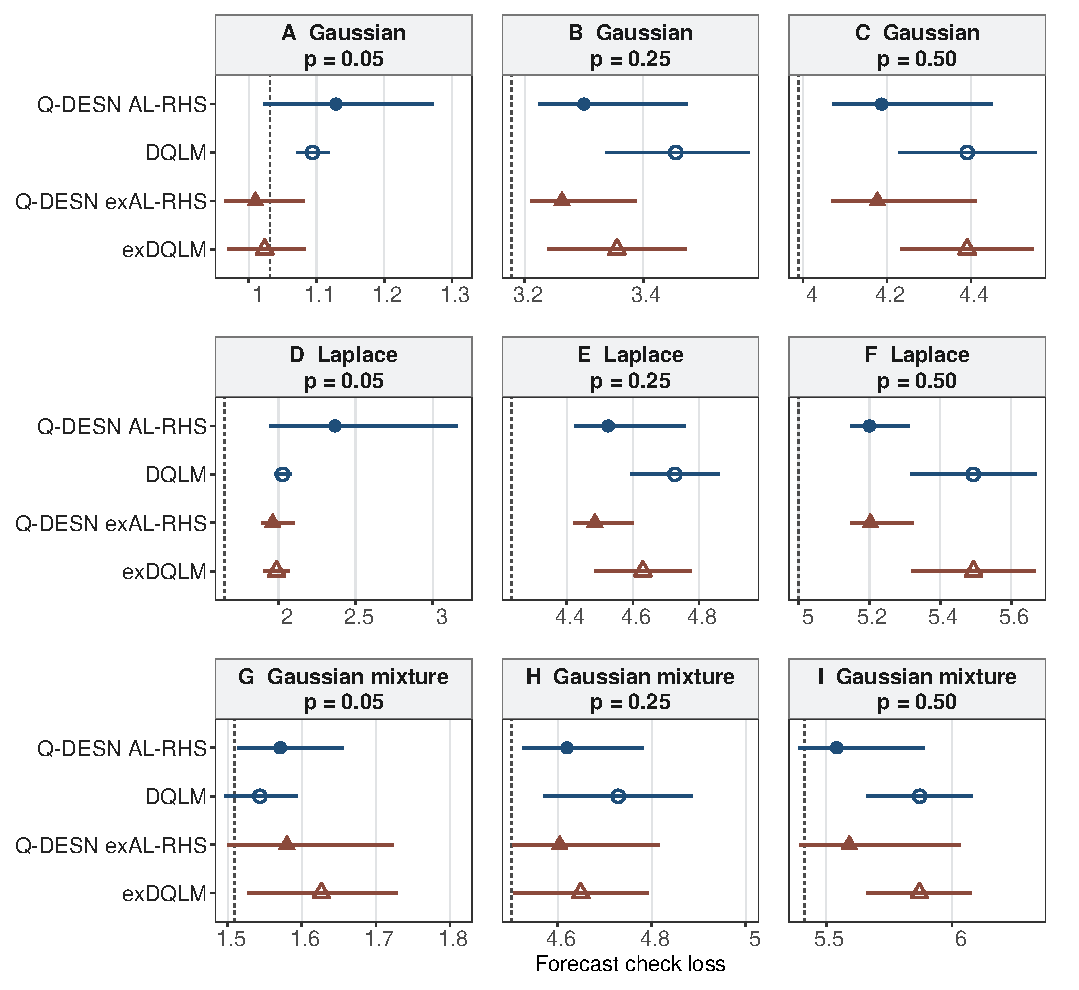
\includegraphics[width=0.98\textwidth]{figures/ch04-qdesn/independent_simulation/independent_train500_eval300_mcmc_forecast_check_v1.pdf}
\caption{MCMC forecast check loss over the first 300 evaluation targets (10 origins). Points and equal-tailed 95\% intervals summarize the draw-wise criterion averaged over scored pairs; lower is better. Navy circles identify \(\AL\) models and muted-brick triangles \(\exAL\) models; filled symbols denote Q--DESN and open symbols their dynamic linear comparators. Panels A--I identify the observation-error family and probability level. The dashed line marks population expected check loss at the true conditional quantile, not a finite-sample lower bound. Panel scales match the 500-target sensitivity figure. Model selection is criterion specific, and forecast draws from competing models are dependent because they share evaluation targets.}
\figalt{Nine panels compare four models using mean forecast check loss and 95 percent intervals over 300 scored targets.}
\label{qdesn2026:fig:simulation-500obs-mcmc-forecast-check-loss-intervals}
\end{figure}


\subsection{Multiquantile simulation design}

The second simulation study compares MQ--DESN with independent Q--DESN at the
seven levels
\(p_k\in\{0.05,0.10,0.25,0.50,0.75,0.90,0.95\}\)
under the \(\AL\) and \(\exAL\) likelihoods. Eight mechanisms vary the
response distribution and temporal dynamics. Within each mechanism, one
DESN and RHS specification is selected using separate simulated series and
held common across the four regressions. Each regression then uses 500
fitting observations, followed by forecast evaluation.

The comparison spans 33 origins and 30 horizons per origin, giving 990 common
origin--horizon pairs from one evaluation trajectory per mechanism. These
pairs are temporally dependent and are not independent simulation replications.
At each origin, observed history initializes the
reservoir, and future responses are generated recursively. Oracle
\(\aCRPS\), defined in Eq.~\eqref{qdesn2026:eq:dgp-integrated-score-main}, evaluates
the quantile forecasts against the known conditional response distribution.
The reported intervals summarize posterior uncertainty in the score averaged
over these pairs, conditional on the realized trajectory, fitted model, and
averaged future predictors defined in
Section~\ref{qdesn2026:sec:forecast}. Appendix~\ref{app:qdesn-simulation-support}
gives the generating mechanisms and sensitivity to
draw-specific recursive forecasting.

\subsection{Multiquantile results}

Figure~\ref{qdesn2026:fig:joint-qdesn-pure-desn-v2-forecast-acrps} shows the posterior
score comparison. MQ--DESN under exAL has the lowest mean for asymmetric
tails and MQ--DESN under AL for Gaussian dynamics. Independent Q--DESN
under AL is lowest for
Gaussian-mixture, Laplace, nonlinear-reservoir, persistent-heavy-tail, and
Student-\(t\) mechanisms; independent Q--DESN under exAL is lowest for regime shifts.
The marginal intervals of the numerical winner and runner-up overlap in
every mechanism.

\begin{figure}[!htbp]
\centering
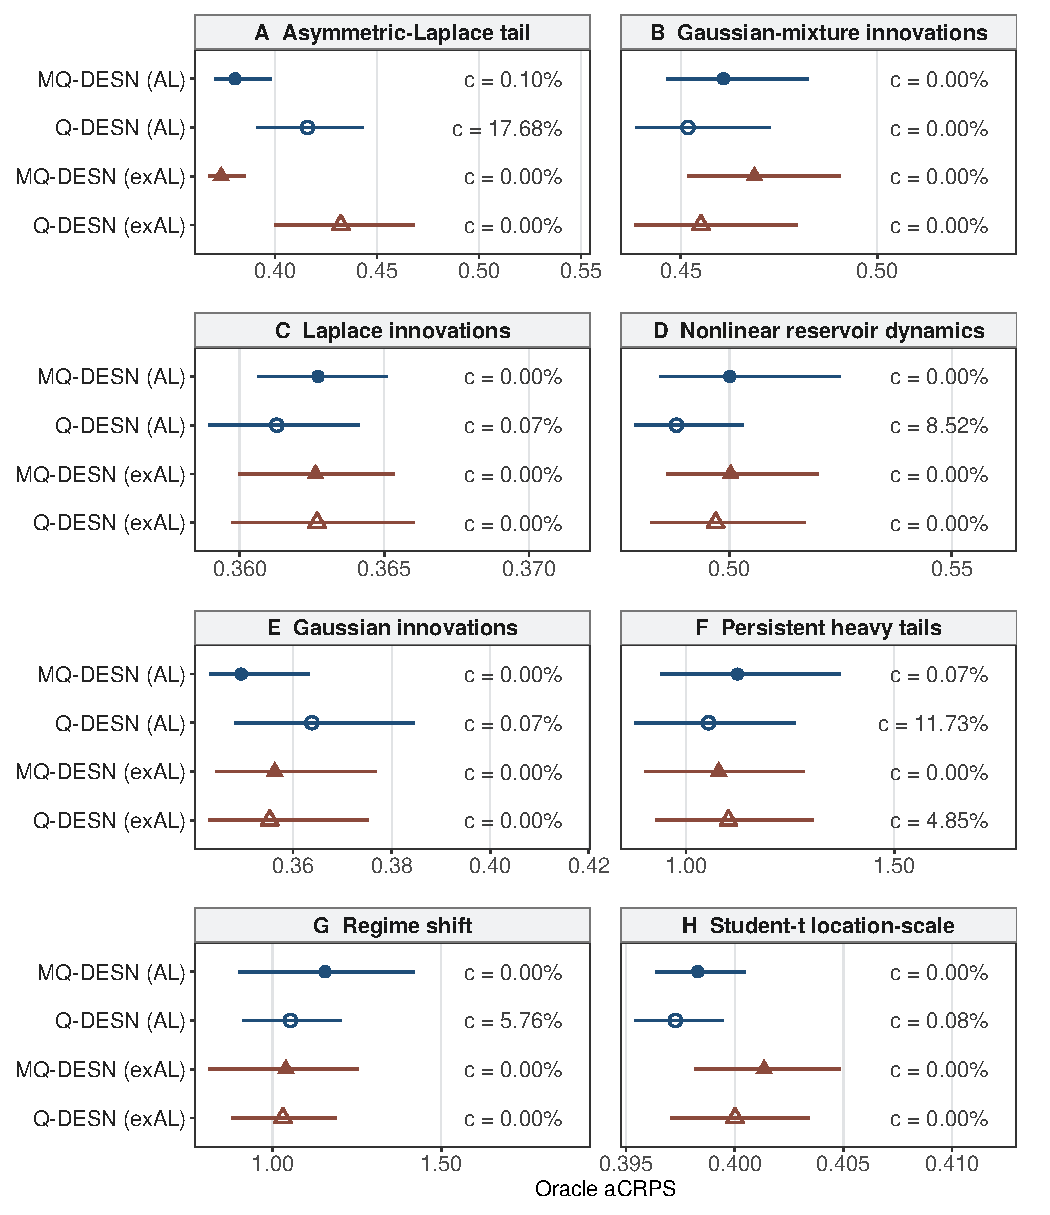
\includegraphics[width=0.94\textwidth]{figures/ch04-qdesn/joint_qdesn_simulation/joint_qdesn_pure_desn_v2_mq_forecast_dgp_acrps.pdf}
\caption{Oracle finite-grid \(\aCRPS\) in the multiquantile study. Points are posterior means and segments are equal-tailed 95\% intervals for the score averaged over the common forecast pairs, conditional on each model's averaged future predictors. Lower scores are better. Annotations \(c\) give raw adjacent-level crossing percentages for posterior-mean forecast grids. Q--DESN fits levels independently; MQ--DESN estimates their coefficients jointly. The scored grids use the monotone transformation specified in the integrated technical material.}
\label{qdesn2026:fig:joint-qdesn-pure-desn-v2-forecast-acrps}
\end{figure}


Across 47,520 adjacent-level comparisons per model, the raw crossing rates of
the posterior-mean forecast grids are 0.021\% for MQ--DESN (AL), 5.488\% for
Q--DESN (AL), 0\% for MQ--DESN (exAL), and 0.606\% for Q--DESN (exAL).
MQ--DESN under exAL has no raw crossings in any of the eight mechanisms.
Both multiquantile coefficient sharing and the exAL likelihood are associated
with fewer crossings in this comparison. The improvement in ordering is
more consistent than the score gains: independent regressions have the
lowest mean oracle score in six mechanisms, whereas MQ--DESN leads for
Gaussian and asymmetric-tail dynamics. Appendix~\ref{app:qdesn-simulation-support}
gives the recursive-feature sensitivity and its uncertainty interpretation.

\section{Application: streamflow quantile forecast correction}
\label{qdesn2026:sec:data}

Daily river-discharge measurements from the United States Geological Survey
(USGS) provide a local reference for assessing hydrological forecasts.
The Global Flood Awareness System (GloFAS) combines meteorological
information with hydrological modeling to produce historical discharge
estimates and ensemble forecasts for flood early warning
\citep{qdesn-AlfieriEtAl2013GloFAS,qdesn-HarriganEtAl2023GloFASForecasts,qdesn-CEMS2026GloFASDocumentation}. Their distributions can differ from those
observed at an individual gauge. We study these differences for the San
Lorenzo River at Big Trees, California, using historical USGS and GloFAS
records to learn quantile-specific discrepancies. Combining this regression
with the issued ensemble gives corrected forecasts of reference-streamflow
quantiles.

\subsection{Data and forecasting problem}

Discharge is analyzed on the \(\log(1+\mathrm{flow})\) scale, with flow
measured in \(\mathrm{m}^3/\mathrm{s}\) before transformation. Write
\(y_t\) for transformed USGS discharge and \(g_t^{\mathrm{ret}}\) for the
transformed historical GloFAS estimate. At the forecast origin \(T\),
\GlofasApplicationCurrentOriginDate{}, GloFAS provides 51 ensemble
members for the following \GlofasApplicationCurrentScoredHorizons{} days,
ending on 22~January~2023. Let \(g_{T+h,e}^{\mathrm{ens}}\) denote member
\(e\) at horizon \(h\), on the same transformed scale.

Precipitation predictors come from the Parameter-elevation Regressions on
Independent Slopes Model (PRISM), and soil-moisture predictors from ERA5,
the fifth-generation reanalysis of the European Centre for Medium-Range
Weather Forecasts (ECMWF). Both use realized values during the forecast
window; future USGS measurements are reserved for scoring.
Appendix~\ref{app:qdesn-glofas-support} records the historical selection and
forecast-window information boundary.

\subsection{Quantile-based forecast correction}

Two fixed DESN feature maps represent the reference process and the
GloFAS-minus-USGS discrepancy. For probability level \(p\), write
\(q_{p,t}=\vect x_t^{\mathrm{ref}\top}\vect\beta_p\) for the reference
quantile and \(d_{p,t}=\vect x_t^{\mathrm{disc}\top}\vect\delta_p\) for the
level-specific location adjustment. Under AL, the historical and issued
likelihoods have the locations
\begin{equation}
\begin{aligned}
\text{Reference history:}\quad
y_t\mid\cdot&\sim\AL_p(q_{p,t},\sigma_Y),\\
\text{Retrospective GloFAS:}\quad
g_t^{\mathrm{ret}}\mid\cdot&\sim\AL_p(q_{p,t}+d_{p,t},\sigma_G),\\
\text{Issued member:}\quad
g_{T+h,e}^{\mathrm{ens}}\mid\cdot&\sim
\AL_p(q_{p,T+h}+d_{p,T+h},\sigma_G).
\end{aligned}
\label{qdesn2026:eq:glofas-part4-main}
\end{equation}
The unknown future reference path is treated as latent and enters the lagged
inputs to both DESN feature maps. Issued members inform this path through the
location relation in Eq.~\eqref{qdesn2026:eq:glofas-part4-main}, with equal weights
totaling one at each horizon. Appendix~\ref{app:qdesn-glofas-support} specifies the weighted
augmentation and latent-path approximation.

The comparison uses the seven levels \(0.05\), \(0.20\), \(0.35\), \(0.50\),
\(0.65\), \(0.80\), and \(0.95\). Q--DESN fits the levels separately under
AL or exAL; MQ--DESN applies adjacent-quantile RHS shrinkage within the
reference and discrepancy coefficient paths. The exAL families replace the
AL likelihood in Eq.~\eqref{qdesn2026:eq:glofas-part4-main} by its shape-extended
counterpart. Gaussian DESN baselines with ridge or RHS regularization and the
raw GloFAS ensemble complete the comparison.

The reservoir and prior specifications were selected using historical
development and confirmation periods, without using the held-out issued
window. Posterior inference then accounts for the regression parameters
and the latent future streamflow path. The long historical record and
high-dimensional regressions make MCMC computationally demanding, so we
use VB to approximate this posterior. Appendices~\ref{app:qdesn-computation}
and~\ref{app:qdesn-glofas-support} describe the approximation and the
convergence criteria satisfied by both MQ--DESN fits.

\subsection{Forecast correction results}

Table~\ref{qdesn2026:tab:glofas-application-score} gives the complete seven-family
comparison on the same issued window. Q--DESN under AL is the descriptive
leader, with grid \(\aCRPS\) of \GlofasApplicationCurrentQdesnAcrps{},
compared with \GlofasApplicationCurrentRawAcrps{} for raw GloFAS.
Q--DESN under exAL and Gaussian DESN with ridge regularization have the next
lowest scores; Gaussian DESN with RHS regularization scores worse than raw GloFAS.

Score and calibration give different assessments. Q--DESN under AL has
coverage of 21 of 28 observations for the nominal 90\% interval. MQ--DESN under AL
covers 22, the largest count among fitted families, but both fall below the
nominal proportion. Gaussian DESN with ridge regularization covers only
3 of 28, despite its relatively low score. Only 8 of 28 observations fall
below the MQ--DESN exAL forecast at level 0.95.
All seven reported issued-window quantile grids are ordered without a
crossing correction. Appendix~\ref{app:qdesn-glofas-support} reports the
level-specific calibration evidence.

Figure~\ref{qdesn2026:fig:glofas-application-forecast-period} shows the observations and
issued ensemble, followed by Q--DESN under AL and the illustrative Gaussian ridge
baseline over the same historical and forecast window and on a common vertical
scale. Appendix~\ref{app:qdesn-glofas-support} retains the calibration
diagnostic that qualifies the score ranking.

\begin{table}[!htbp]
\centering
\TableStyle
\caption{Quantile forecast correction at the 25 December 2022 origin. Scores use the
28 issued horizons on the \(\log(1+\mathrm{flow})\) scale, with flow in
\(\mathrm{m}^3/\mathrm{s}\), and the grid
\(0.05,0.20,0.35,0.50,0.65,0.80,0.95\).
Mean check loss weights the seven levels equally; grid \(\aCRPS\) uses
the unnormalized trapezoidal weights in Eq.~\eqref{qdesn2026:eq:acrps-main}.
Coverage is the observed proportion between the reported 0.05 and 0.95
quantiles. All seven models are evaluated on the same dates; lower scores
are better.}
\label{qdesn2026:tab:glofas-application-score}
\input{\GlofasApplicationCurrentScoreTable}
\end{table}

\begin{figure}[!htbp]
\centering
\includegraphics[width=0.94\textwidth]{\GlofasApplicationCurrentForecastWindowFigure}
\caption{Streamflow data and two quantile forecasts at the
25 December 2022 origin. (a) USGS observations, retrospective GloFAS, and all
51 issued ensemble paths. (b) Q--DESN (AL) and (c) Gaussian DESN (ridge) show seven
quantile levels over the same 30 historical days and 28 issued horizons.
Before the origin, curves are posterior-mean fitted conditional quantiles;
afterward, they show forecasts informed by the issued ensemble. Axes are common, and
the vertical dashed line marks the origin.
Filled green points denote historical USGS; open dark-red points are used
only for evaluation. Orange identifies GloFAS products. Blue curves show
the quantile levels, with the median emphasized.
The outer paths bound a nominal 90\% quantile interval, not a credible band;
no crossing correction is applied. The analysis conditions on realized
future weather.}
\figalt{Three stacked panels share a vertical scale. The first shows green
filled historical USGS points, orange retrospective GloFAS and 51 issued
ensemble paths, and dark-red open held-out USGS points. The second and third
show seven blue quantile curves for Q--DESN (AL) and Gaussian DESN (ridge) over
the same 30 historical and 28 forecast dates. Historical and held-out points
are repeated, and all three panels share the date range and forecast-origin
line.}
\label{qdesn2026:fig:glofas-application-forecast-period}
\end{figure}

% Finish the streamflow displays before introducing the next application.

\section{Application: electricity-price quantile forecasting}
\label{qdesn2026:sec:pricefm-application}

Day-ahead electricity prices vary with demand, renewable generation, and
exchange between connected markets. Conditional quantiles describe the
associated price uncertainty. Foundation models use pretraining to learn
representations that can be reused across related series. PriceFM specializes
this approach to probabilistic electricity-price forecasting with regional
covariates and transmission-network information \citep{qdesn-YuEtAl2026PriceFM}.
Its authors also provide a European benchmark, which we use to compare
independent Q--DESN forecasts with the released PriceFM predictions.
Version~4 contains day-ahead price records and load, solar, and wind forecast
covariates at 15-minute
resolution from 1~January~2022 through 1~January~2026.

\subsection{Comparison design}

The comparison contains \PricefmFullRegionFolds{} region--fold evaluations,
spanning \PricefmFullRegions{} European bidding regions and
\PricefmFullFolds{} rolling folds. For each region, one Q--DESN specification
was selected using temporal development periods within the first fitting
interval. The first outer development period determined the AL or exAL family.
The DESN specification, shrinkage settings, predictors, and AL or exAL
likelihood were then held fixed across that region's three evaluation folds.
Each daily forecast origin has 96 quarter-hourly targets.

Each evaluation is scored on the fold-aligned held-out timestamps and
probability levels \PricefmFullPaperQuantiles. We use average quantile loss
(AQL) to compare forecasts. Throughout this section,
\(\Delta\) AQL denotes Q--DESN AQL minus PriceFM AQL. Negative values indicate
lower Q--DESN AQL; positive values indicate lower PriceFM AQL.
For region \(r\) and fold \(f\), with \(N_{r,f}\) scored timestamps, the score is
\begin{equation}
\text{Average quantile loss:}\quad
\operatorname{AQL}_{r,f}
=\frac{1}{N_{r,f}K}\sum_{i=1}^{N_{r,f}}\sum_{k=1}^{K}
\rho_{p_k}\!\left(y_{r,f,i}-\widehat q_{r,f,i,k}\right),
\label{qdesn2026:eq:pricefm-aql-main}
\end{equation}
where \(K=7\) and both outcomes and forecasts are in euros per megawatt-hour
(EUR/MWh).
Unlike \(\aCRPS\), AQL equally weights the probability levels and has no
factor of two. Aggregate scores give equal weight to the 114 region--fold
evaluations, rather than pooling all timestamps.

The predictors include the released load, solar, and wind forecast
covariates; spatial specifications also use neighboring-region features or
their summaries. Their issue-time vintages were not independently verified.
Appendix~\ref{app:qdesn-pricefm-support} records the fitting-period selection
history and its information-availability limitation.

\subsection{Results}

The mean Q--DESN AQL is
\PricefmFullMeanQdesnAql{}, compared with \PricefmFullMeanPricefmAql{} for
PriceFM, giving mean \(\Delta\) AQL \PricefmFullMeanDeltaAql{}.
Q--DESN has lower AQL in \PricefmFullQdesnWins{} of
\PricefmFullRegionFolds{} comparisons, but its aggregate loss is slightly
higher. Table~\ref{qdesn2026:tab:pricefm-matched-aql-comparison} shows the variation
across folds: Q--DESN is marginally lower in the second fold, whereas
PriceFM is lower in the first and third. Appendix~\ref{app:qdesn-pricefm-support} reports regional
comparisons and the historical sensitivity analysis.

\begin{table}[!htbp]
\centering
\caption{Matched electricity-price forecast comparison. Entries are unweighted
summaries across region--fold evaluations,
overall and by fold. The Q--DESN specification for each region was selected
using fitting and development data and held fixed across its three evaluation folds.
Here \(\Delta\) AQL is Q--DESN minus PriceFM, so negative values favor Q--DESN.
AQL is in EUR/MWh; all scores use matched held-out timestamps and the same
seven probability levels.}
\label{qdesn2026:tab:pricefm-matched-aql-comparison}
\begingroup
\TableStyle
\scriptsize
\setlength{\tabcolsep}{3pt}
\begin{tabular}{@{}lrrrrrrr@{}}
\toprule
Comparison set & $n$ & \shortstack{Q--DESN\\lower} & \shortstack{PriceFM\\lower} & \shortstack{Mean\\Q--DESN AQL} & \shortstack{Mean\\PriceFM AQL} & \shortstack{Mean\\$\Delta$} & \shortstack{Median\\$\Delta$} \\
\midrule
Overall & 114 & 54 & 60 & 7.217 & 7.039 & 0.178 & 0.071 \\
Fold 1 & 38 & 18 & 20 & 7.353 & 7.297 & 0.056 & 0.084 \\
Fold 2 & 38 & 24 & 14 & 6.799 & 6.826 & -0.027 & -0.155 \\
Fold 3 & 38 & 12 & 26 & 7.499 & 6.993 & 0.506 & 0.247 \\
\bottomrule
\end{tabular}
\endgroup

\end{table}

% ============================================================

\section{Discussion}
\label{qdesn2026:sec:discussion}

Q--DESN retains a regularized linear regression for the quantile location
while using fixed recurrent features to represent nonlinear temporal
dependence. Its posterior concerns the regression, likelihood, and shrinkage
parameters, conditional on the reservoir. This distinction makes the model
accessible through Bayesian regression calculations without treating every
network weight as an unknown parameter. The AL augmentation supports
Gibbs-based computation, while VB makes repeated regression fits practical.

The development-informed single-quantile comparison is most favorable to Q--DESN at the median,
with likelihood preferences varying by observation-error family. In the
multiquantile study, MQ--DESN improves the ordering of posterior-mean
forecast grids, especially under exAL, while independent regressions have
lower mean oracle scores in most mechanisms. These results distinguish the
benefit of adjacent-coefficient regularization for quantile ordering from its
less consistent gains in forecast scores.

The applications illustrate different uses of the regression. For streamflow
correction, the reference--discrepancy regression combines gauge measurements
with GloFAS products at one retrospective forecast origin. Q--DESN under AL
has the lowest descriptive issued-window
score, but its nominal 90\% interval covers 75\% of the issued-window
observations. The electricity-price comparison holds each regional
specification fixed across three evaluation folds and has slightly higher aggregate
AQL than PriceFM, with substantial fold and region variation. The
applications retain their stated information sets: realized weather for
streamflow correction and supplied covariates with unverified issue-time
vintages for electricity prices.

Further work should assess variation across repeated simulated series and
uncertainty from reservoir selection and recursively generated predictors.
Multi-origin GloFAS evaluation with covariates available at issuance and
paired PriceFM uncertainty analyses would extend the present comparisons.

\chapter{Mean-tilted intervals and calibrated tolerance inference}
\label{ch:research-d}

\begin{singlespace}
\noindent\textit{This chapter is based on two closely related projects by Antonio de Leon, Raquel Prado, and Bruno Sans\'o. The main argument develops the population foundations and calibrated profiled MTI procedure; a final section states the proposed regression and dynamic endpoint extensions. The supporting proofs, calibration record, and computational derivations appear in Sections~\ref{app:mti-proofs}, \ref{app:mti-calibration}, and~\ref{app:mti-extensions} of Appendix~\ref{app:mti-technical}.}
\end{singlespace}

\section{Introduction}
\label{rqr2026:sec:introduction}

A prescribed probability content defines a class of possible intervals. Equal-tailed,
shortest-contiguous, and other intervals may contain the same population fraction
while placing their endpoints in different parts of the distribution. Tolerance
intervals add a second requirement: with confidence \(1-\alpha\), the reported
random interval should contain at least content \(c\) of the population
\citep{rqr-Wilks1941ToleranceLimits,rqr-Wilks1942StatisticalPrediction,rqr-Robbins1944DistributionFreeTolerance}.
Thus content, placement, and repeated-sampling confidence are separate parts of
the problem. Fitting the two conditional quantiles at \((1-c)/2\) and
\((1+c)/2\) is appropriate for a central equal-tailed target
\citep{qdesn-KoenkerBassett1978}. Shortest-interval and mean-preserving questions
require different functionals, so their validation should be aligned with the
interval being estimated \citep{rqr-BrehmerGneiting2021Intervals,rqr-FisslerEtAl2021SetValued}.

Pouplin et al. introduced a residual-product criterion under the name Relaxed
Quantile Regression \citep{rqr-PouplinEtAl2024RQR}. The loss depends on
\((y-\eta_1)(y-\eta_2)\), whose sign records whether \(y\) lies between two raw
roots. The population score equations identify the unrestricted regular target:
among contiguous intervals with content \(c\), the minimizer is the interval
whose retained mean equals the population mean. We call this target the
mean-preserving interval (MPI). The terminology is descriptive; the original
residual-product construction is due to Pouplin et al.

The same score structure gives a placement family. The mean-tilted interval
(MTI) loss keeps the MPI content score and replaces retained-mean equality by a
fixed retained-mean offset \(\delta\). MPI is the \(\delta=0\) member of the
family. Nonzero tilts move the interval within the content-\(c\) class, and the
equal-tailed and shortest-contiguous intervals correspond to
distribution-specific tilts. The tilt is therefore part of the target
specification, or it is selected by a separate calibration rule before empirical
claims are made.

This target geometry suggests a tolerance procedure that searches over fitted
content and interval placement. For each candidate content \(q>c\) and tilt
\(\delta\), a deterministic profile calculation estimates endpoints under the
MTI generalized-posterior criterion. A separate Dirichlet-process (DP)
response-distribution posterior supplies a content-probability check, and the
shortest eligible fitted interval is reported.
The fitted content \(q\) allows for sampling uncertainty about the required
population content \(c\), while the tilt controls placement.

The candidate grid is specified before calibration. A uniform-scan retained
fraction provides a reference for fitted content, and the grid is refined
to represent every intervening order-statistic rank of the profiled radius.
Separate simulation samples determine a posterior probability cutoff for each
sample-size/content setting. Selection requires simultaneous lower confidence
bounds for content attainment of at least the requested tolerance confidence
across the eight calibration distributions. The resulting fixed rule is then
evaluated on independent samples. These calculations provide evidence for the
specified distributional panel; a distribution-free guarantee for the selected
interval requires further theory. The same loss also supports proposed
generalized-Bayes endpoint regression, basis-expansion endpoint models, and
time-varying endpoint models. These extensions are summarized after the
tolerance study and derived in Section~\ref{app:mti-extensions}; they do not
inherit its empirical calibration.

The contributions are as follows. First, the residual-product loss is shown to
target MPI, and MTI is shown to generalize MPI by indexing admissible contiguous
fixed-content windows through retained-mean tilt. Second, this geometry is used
to construct a calibrated MTI tolerance procedure that searches over fitted
content and tilt. Third, an independent validation study compares MTI,
Young--Mathew interpolation, and Wilks
intervals across feasible sample-size/content cells and a distributional panel
chosen to include symmetric, heavy-tailed, and strongly skewed cases.
Finally, a pharmaceutical-manufacturing application illustrates endpoint
placement on historical batch data using the same prespecified rules.

The tolerance study concerns iid continuous univariate samples. The population
MTI characterizations and the fixed-interval DP content law hold under their
respective assumptions; the reported tolerance performance is empirical.
Regression-family and dynamic tolerance
calibration require additional theory. Generalized-posterior endpoint summaries
are loss-based summaries of interval-root functionals; response prediction would
require a separate response-distribution model. Proper scoring rules remain useful when their target matches the
forecast object \citep{exd-gneiting2007,qdesn-Gneiting2011,qdesn-GneitingKatzfuss2014};
the usual interval score targets an equal-tailed interval and is secondary here
\citep{rqr-BrehmerGneiting2021Intervals}.

The chapter proceeds as follows. Section~\ref{rqr2026:sec:interval-functionals} defines
the fixed-content interval class. Sections~\ref{rqr2026:sec:mpi-loss}
and~\ref{rqr2026:sec:mti-loss} identify the MPI target and the MTI placement family.
Section~\ref{rqr2026:sec:static-theory-statements} records the empirical balance
identity and the fixed-target generalized-Bayes criterion used in the validation study.
Section~\ref{rqr2026:sec:mti-tolerance} defines the calibrated MTI tolerance procedure
and its scan reference. Section~\ref{rqr2026:sec:evaluation} gives the independent
validation design, and Section~\ref{rqr2026:sec:pharma-application} presents the
pharmaceutical application. A compact extension section then connects the
fixed-target loss to regression and dynamic endpoints before the unified
discussion in Section~\ref{rqr2026:sec:discussion}.

\section{Fixed-content interval targets}
\label{rqr2026:sec:interval-functionals}

Let \(Y\) have a nondegenerate continuous distribution with finite mean
\(\mu\) and strictly increasing quantile function \(Q\) on \((0,1)\). Apart
from probability-zero subsets outside the support, every contiguous interval
of content \(c\) can be represented by the probability window
\[
I_c(u)=[Q(u),Q(u+c)],\qquad 0\le u\le1-c.
\]
Define its retained mean and geometric width by
\[
M_c(u)=\frac{1}{c}\int_u^{u+c}Q(v)\,dv,\qquad
W_c(u)=Q(u+c)-Q(u).
\]
Probability content fixes the length of the window on the probability scale,
but not its lower-tail index \(u\). We use ET for equal-tailed, MPI for
mean-preserving, and SH for shortest-contiguous intervals.
Table~\ref{rqr2026:tab:interval-functionals} summarizes these three principal
placement rules.
\begin{table}[h!]
\centering
\caption{\textbf{Three contiguous fixed-content interval functionals.}}
\label{rqr2026:tab:interval-functionals}
\TableStyle
\begin{tabularx}{\textwidth}{@{}>{\raggedright\arraybackslash}p{0.19\textwidth}
  >{\raggedright\arraybackslash}X
  >{\raggedright\arraybackslash}X@{}}
\toprule
Target & Probability-window rule & Placement principle\\
\midrule
Equal-tailed
& \(u=(1-c)/2\)
& Equal omitted tail probabilities\\
MPI
& \(M_c(u)=\mu\)
& Mean-preserving truncation\\
Shortest contiguous
& \(u\in S_{\mathrm{SH}}=\argmin_v W_c(v)\)
& Minimum geometric width\\
\bottomrule
\end{tabularx}
\end{table}
For a regular interior shortest interval under a positive density,
\(f\{Q(u)\}=f\{Q(u+c)\}\). Under multimodality, a highest-density region may
be disconnected, whereas the targets above remain contiguous
\citep{rqr-BrehmerGneiting2021Intervals}. Figure~\ref{rqr2026:fig:three-interval-principles}
compares the three principal balance conditions for one strongly asymmetric
distribution.

\begin{figure}[H]
\centering
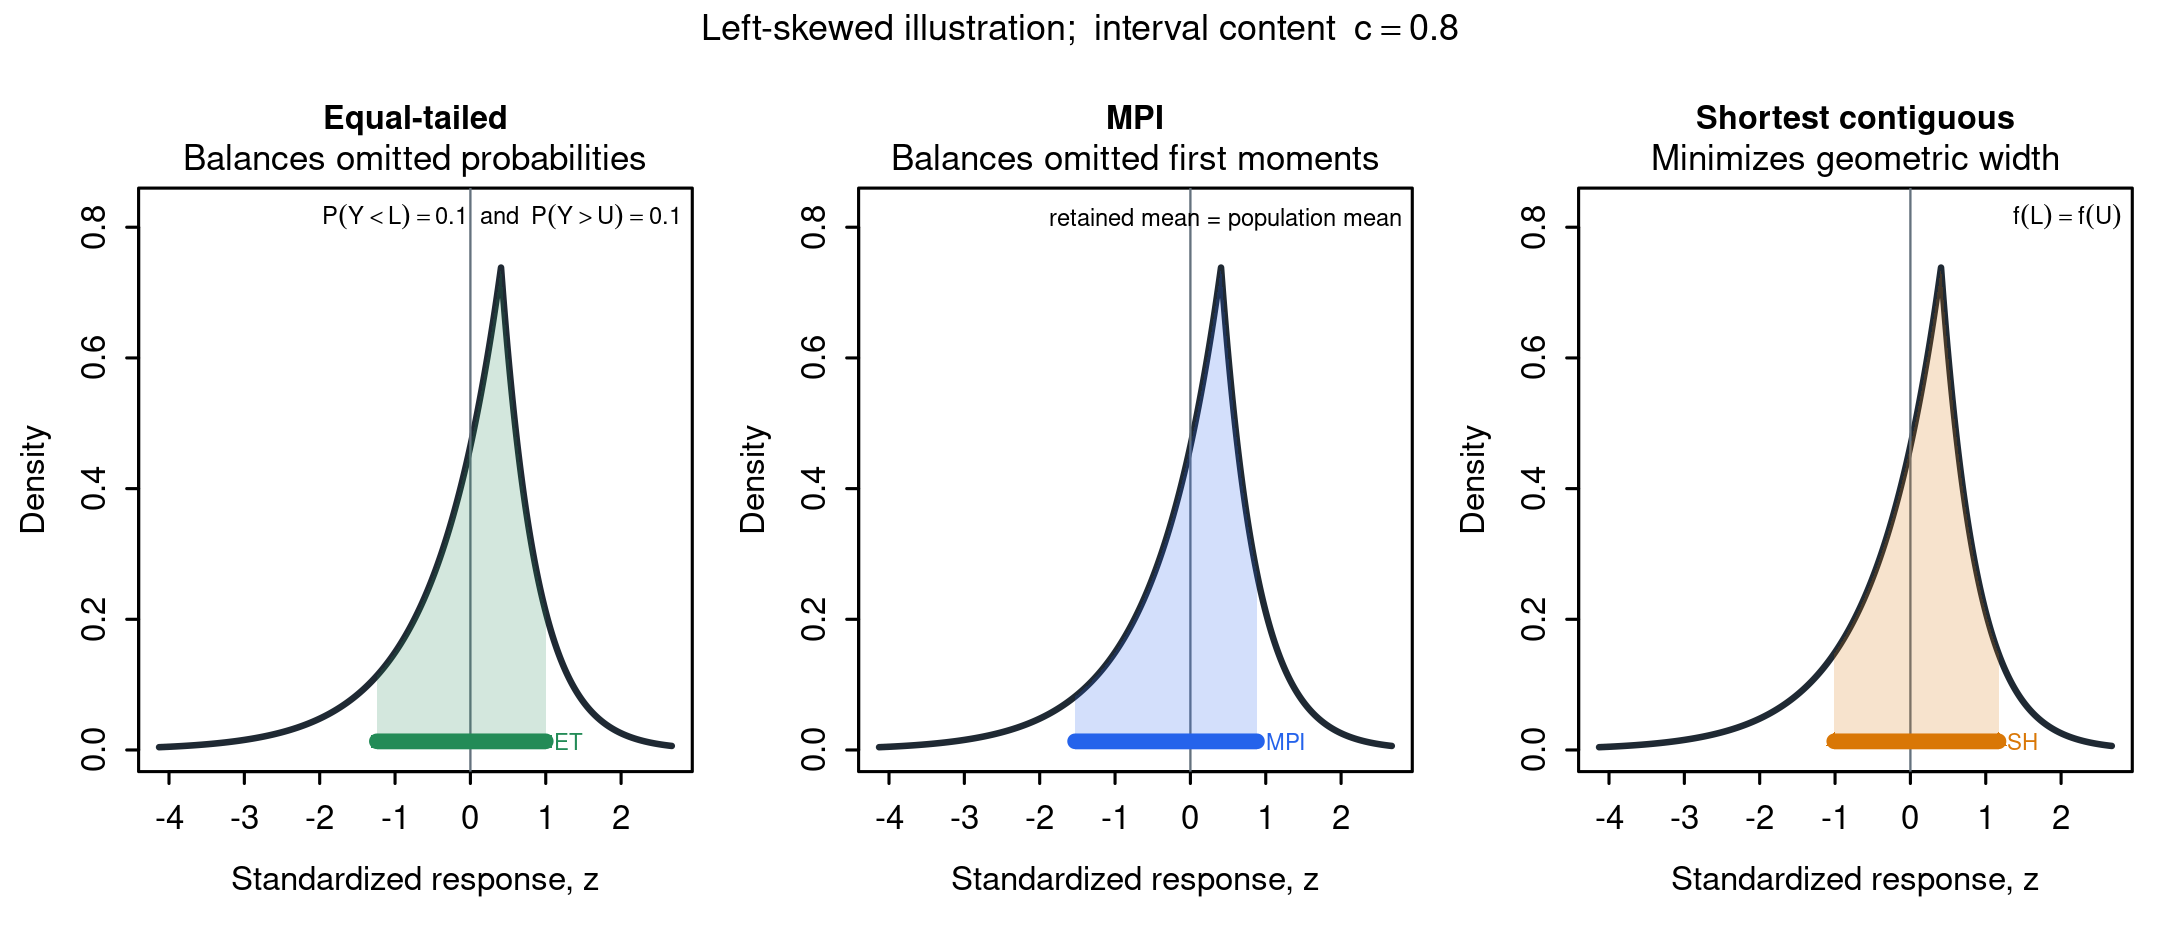
\includegraphics[width=\textwidth]{figures/ch05-mti/generated/fig01_three_balance_principles.png}
\caption{\textbf{Three interval-selection principles under left skewness.}
All panels use the same continuous left-skewed population illustration with
content \(c=0.80\), displayed after standardization. Equal-tailed (ET)
intervals balance omitted probabilities, MPI balances omitted first
moments, and shortest-contiguous (SH) intervals minimize geometric width.
These deterministic population calculations compare functionals; they are not
finite-sample or comparative-performance evidence.}
\label{rqr2026:fig:three-interval-principles}
\end{figure}

\section{The mean-preserving interval target}
\label{rqr2026:sec:mpi-loss}

The residual-product loss becomes a statistical procedure once its target is
identified. This section first defines the pointwise loss, then shows that its
regular unrestricted population solution is the mean-preserving member of the
fixed-content interval class.

Fix a desired interval content \(c\in(0,1)\) and ordered endpoints \(a<b\).
The pointwise MPI loss is
\begin{equation}
\ell_c^{\mathrm{MPI}}(a,b;y)=
\begin{cases}
(1-c)(y-a)(b-y), & a<y<b,\\
c(y-a)(y-b), & y\le a\ \text{or}\ y\ge b.
\end{cases}
\label{rqr2026:eq:mpi-loss-piecewise}
\end{equation}
Both branches are nonnegative and meet continuously at zero when \(y=a\) or
\(y=b\). An observation inside the interval is weighted by \(1-c\), whereas a
miss is weighted by \(c\). The two factors also encode distance from both
endpoints, so the criterion weights membership and endpoint displacement
together. Increasing \(c\) raises the relative cost of a miss; at a regular
population optimum, this weighting
produces the content equation established below. For data
\(y_1,\ldots,y_n\), MPI minimizes
\(\sum_{i=1}^n\ell_c^{\mathrm{MPI}}(a,b;y_i)\), or the corresponding regression
loss when the two endpoints depend on predictors.

The familiar check-loss notation gives an equivalent compact representation.
For a scalar argument \(r\), let
\[
\rho_c(r)=r\{c-\ind(r<0)\}
=
\begin{cases}
(1-c)|r|, & r<0,\\
cr, & r\ge0.
\end{cases}
\]
Now define the product residual
\[
e(a,b;y)=(y-a)(y-b).
\]
Because \(e(a,b;y)<0\) exactly when \(a<y<b\),
\begin{equation}
\ell_c^{\mathrm{MPI}}(a,b;y)=\rho_c\{e(a,b;y)\}.
\label{rqr2026:eq:mpi-product-check}
\end{equation}
This representation also makes clear that the loss is symmetric in its two
roots; the ordering \(a<b\) is imposed only to interpret them as lower and
upper endpoints.
The check loss therefore acts on the scalar product residual, not on
\(y-a\) or \(y-b\) separately. In particular, \(c\) is the desired interval
content; it is neither an assigned response-quantile level for either endpoint
nor the generalized-Bayes learning rate.

The midpoint--half-width parameterization makes the interval geometry
explicit. Write \(a=m-h\) and \(b=m+h\), where \(h>0\). Then
\[
e(a,b;Y)=(Y-m)^2-h^2,
\]
so \(e<0\) means that \(Y\) is within distance \(h\) of \(m\). The half-width
and midpoint are estimated jointly by minimizing the expected loss
\(R_c(a,b)=\E\{\ell_c^{\mathrm{MPI}}(a,b;Y)\}\). Its first-order conditions determine both
the interval content and its placement. The loss defines this population
estimand. When a generalized-Bayes update is used later for a fixed target, its
learning rate controls the strength of the loss update rather than the
population content. The results below concern an unrestricted pointwise
population problem. Restricted regression classes generally recover only
design-weighted projections of these identities.

The endpoint scores have two population consequences: they set the interval
content and make the retained conditional distribution preserve the conditional
mean.

\begin{proposition}[Mean-preserving score characterization]
\label{rqr2026:prop:population-characterization}
Fix \(x\) and let \(a<b\). Suppose
\(\E(Y^2\mid X=x)<\infty\), the conditional distribution has no mass at \(a\)
or \(b\), differentiation may be interchanged with conditional expectation,
and \((a,b)\) is an interior stationary point over an unrestricted pointwise
endpoint class. Then the two population first-order conditions imply
\[
\Pr(a<Y<b\mid X=x)=c,
\]
and
\[
\E\{Y\ind(a<Y<b)\mid X=x\}
=c\,\E(Y\mid X=x).
\]
Equivalently,
\[
\E(Y\mid a<Y<b,X=x)=\E(Y\mid X=x).
\]
\end{proposition}

The population content equation is due to
\citet{rqr-PouplinEtAl2024RQR}. The retained-mean equation is a further
consequence of the same first-order system: conditional on \(X=x\), interval
membership has zero covariance with \(Y\). In omitted-tail form, the same
identity balances first-moment mass around the conditional mean:
\[
\E[\{\mu_x-Y\}\ind(Y<a)\mid X=x]
=
\E[\{Y-\mu_x\}\ind(Y>b)\mid X=x],
\qquad \mu_x=\E(Y\mid X=x).
\]
Tail probabilities may differ; MPI balances their first moments around
\(\mu_x\). The retained core and its excluded complement consequently have the
same conditional mean, although the endpoint midpoint may differ from that
mean. Proposition~\ref{rqr2026:prop:supp-convex-order} in
Section~\ref{app:mti-proofs} further shows that the retained core is a mean-preserving
contraction of the full distribution in convex order. A finite first moment is
enough for the retained-mean identity once the endpoint scores are valid. The
stronger second-moment assumption ensures that the expected MPI loss
is finite and supports the profiled-risk analysis. This distinction matters
because the loss grows quadratically in an extreme response.

The next theorem converts the score identities into a quantile-window
functional. This is the object that the unrestricted population loss estimates.

\begin{theorem}[Quantile-window identification]
\label{rqr2026:thm:quantile-window}
In addition to the conditions of
Proposition~\ref{rqr2026:prop:population-characterization}, suppose that \(F_x\) is
continuous and strictly increasing on its support, and let \(Q_x=F_x^{-1}\).
Define
\[
M_{c,x}(u)=\frac{1}{c}\int_u^{u+c}Q_x(v)\,dv,
\qquad 0\le u\le1-c.
\]
Then \(M_{c,x}\) is strictly increasing. There is a unique index \(u_c(x)\)
satisfying
\[
M_{c,x}\{u_c(x)\}=\mu_x.
\]
The nondegenerate unrestricted MPI stationary interval is therefore
\[
a_c(x)=Q_x\{u_c(x)\},\qquad
b_c(x)=Q_x\{u_c(x)+c\}.
\]
If \(F_x\) is symmetric about \(\mu_x\), then
\(u_c(x)=(1-c)/2\), and the MPI and equal-tailed intervals coincide.
\end{theorem}

This theorem identifies the unique regular stationary window.
Theorem~\ref{rqr2026:thm:profiled-mean-tilt} below strengthens that statement to
the unique global expected-loss minimizer by profiling over the half-width.
Section~\ref{app:mti-proofs} proves these results and records the restricted score
equations. Under the connected-support and local positive-density conditions
used in Theorem~\ref{rqr2026:thm:profiled-mean-tilt}, the regular unrestricted
population intervals form a nested path. If the conditional quantile function
is continuous at \(p_{\mu,x}=F_x(\mu_x)\) and
\(Q_x(p_{\mu,x})=\mu_x\), the two endpoints converge to \(\mu_x\) as
\(c\downarrow0\). Without this local support condition, the zero-content
limit may straddle a support gap. At fixed positive content, the midpoint's
role remains interval placement, while the conditional mean is imposed through
retained-mean balance. If the
conditional law has endpoint atoms,
the corresponding directional conditions give
\[
\Pr(a<Y<b\mid X=x)\le c\le\Pr(a\le Y\le b\mid X=x),
\]
so exact open-interval coverage requires endpoint continuity. Coincident roots
reduce the loss to \(c(Y-a)^2\) and target the conditional mean rather than a
nontrivial interval. Exact retained-mean equality is not asserted at endpoint
atoms without a separate joint subgradient and mass-allocation analysis.

MPI therefore targets an interval directly and can accommodate asymmetric
conditional distributions without assigning endpoint quantile levels in
advance. The characterization is pointwise and unrestricted; it holds only
under the stated conditions. Linear and other restricted root classes instead
satisfy design-weighted score equations and need not attain conditional
coverage or mean preservation at every covariate value. Nor does the
finite-sample unbiasedness argument for fixed endpoints apply automatically to
fitted endpoints: the endpoints depend on the data, and the empirical
objective is nonsmooth when an observation coincides with a root. Finite-sample
or asymptotic guarantees require a separate empirical-process argument.

\section{Mean-tilted intervals}
\label{rqr2026:sec:mti-loss}

The MTI family is the fixed-tilt generalization of MPI. It preserves the MPI
content score and replaces the zero retained-mean-balance equation by a fixed
retained-mean tilt \(\delta\), measured in response units. To move through the
content-\(c\) family without changing the coverage score, define
\[
\ell_{c,\delta}^{\mathrm{MTI}}(m,h;y)
=
\rho_c\{(y-m)^2-h^2\}-2c\delta(m-y).
\]
Equivalently,
\[
\ell_{c,\delta}^{\mathrm{MTI}}(a,b;y)
=
\rho_c\{(y-a)(y-b)\}-c\delta(a+b-2y).
\]
The second form shows that the loss remains invariant to exchanging the two
roots. MPI is exactly the \(\delta=0\) member of the MTI family.

This generalization changes placement but not content. The proposition records
that separation explicitly.

\begin{proposition}[Fixed-content mean tilt]
\label{rqr2026:prop:mean-tilt}
Under the regularity conditions of
Proposition~\ref{rqr2026:prop:population-characterization}, a nondegenerate interior
stationary point of the mean-tilted population risk satisfies
\[
\Pr(a_\delta<Y<b_\delta)=c,\qquad
\E(Y\mid a_\delta<Y<b_\delta)=\mu+\delta.
\]
If \(F\) is continuous and strictly increasing on its support, then for every
\(\delta\) strictly between \(M_c(0)-\mu\) and
\(M_c(1-c)-\mu\), its unique interior quantile-window index solves
\[
M_c(u_\delta)=\mu+\delta.
\]
\end{proposition}

The score equations identify stationary points. Global identification follows
by profiling over the unique content-\(c\) radius at each midpoint and
differentiating the profiled risk; Section~\ref{app:mti-proofs} gives the radius and
envelope-derivative argument.

\begin{theorem}[Global identification of the MTI target]
\label{rqr2026:thm:profiled-mean-tilt}
Suppose that the support closure is an interval (possibly with infinite
endpoints), \(F\) is absolutely continuous and strictly increasing between its
support endpoints, its density is positive and continuous on the support
interior, and \(\E(Y^2)<\infty\). Extend \(F\) by zero and one beyond finite
support endpoints. For every tilt satisfying
\[
M_c(0)-\mu<\delta<M_c(1-c)-\mu,
\]
the expected MTI loss has a unique global minimizer over finite ordered
roots. Its probability-window index \(u_\delta\in(0,1-c)\) is the unique
solution of
\[
M_c(u_\delta)=\mu+\delta.
\]
Nondegeneracy gives \(M_c(0)<\mu<M_c(1-c)\), so MPI is the interior
special case \(\delta=0\).
\end{theorem}

Finite second moments make both endpoint tilt values finite, even when a
support endpoint is infinite. Boundary tilts correspond to one-sided
probability-window limits. Infinite support endpoints lead to semi-infinite
limiting intervals, and finite endpoints require a support constraint to choose
a unique inactive-root representation. Outside the closed admissible tilt range,
the unrestricted risk is unbounded below along the corresponding escaping-root
direction. A proper Gaussian prior can nevertheless yield a proper
finite-sample generalized posterior.

The recovery tilts translate familiar placement rules into the MTI coordinate.
There are three distinct uses of the tilt notation. A fixed target tilt is
chosen before generalized-posterior computation; a population recovery tilt
identifies which \(\delta\) reproduces a familiar interval functional under a
known distribution; an empirical plug-in tilt estimates such a value through a
separate target-selection rule.

\begin{corollary}[Recovery tilts for familiar interval functionals]
\label{rqr2026:cor:recovery-tilts}
MPI is recovered by \(\delta_{\mathrm{MPI}}=0\). Define
\[
S_{\mathrm{SH}}
=
\argmin_{0\le u\le1-c}W_c(u),\qquad
\Delta_{\mathrm{SH}}
=
\{M_c(u)-\mu:u\in S_{\mathrm{SH}}\}.
\]
The population recovery tilt for the equal-tailed interval is
\[
\delta_{\mathrm{ET}}=M_c\{(1-c)/2\}-\mu.
\]
Each \(u\in S_{\mathrm{SH}}\) has recovery tilt
\(\delta_{\mathrm{SH}}(u)=M_c(u)-\mu\). Singular notation is used only when the
shortest-contiguous window is unique or one minimizer has been selected.
\end{corollary}

At regular interior points where the endpoint quantiles are differentiable
and have positive densities,
\[
\frac{du_\delta}{d\delta}=\frac{c}{W_c(u_\delta)},\qquad
\frac{dW_c(u_\delta)}{d\delta}
=\frac{c\,W_c'(u_\delta)}{W_c(u_\delta)}.
\]
Thus an interior width minimum along the tilt path satisfies the usual
equal-endpoint-density condition.
Figure~\ref{rqr2026:fig:mean-tilt-map} visualizes the same recovery map across
symmetric and skewed population laws before adding any finite-sample
approximation layer.

\begin{figure}[!htbp]
\centering
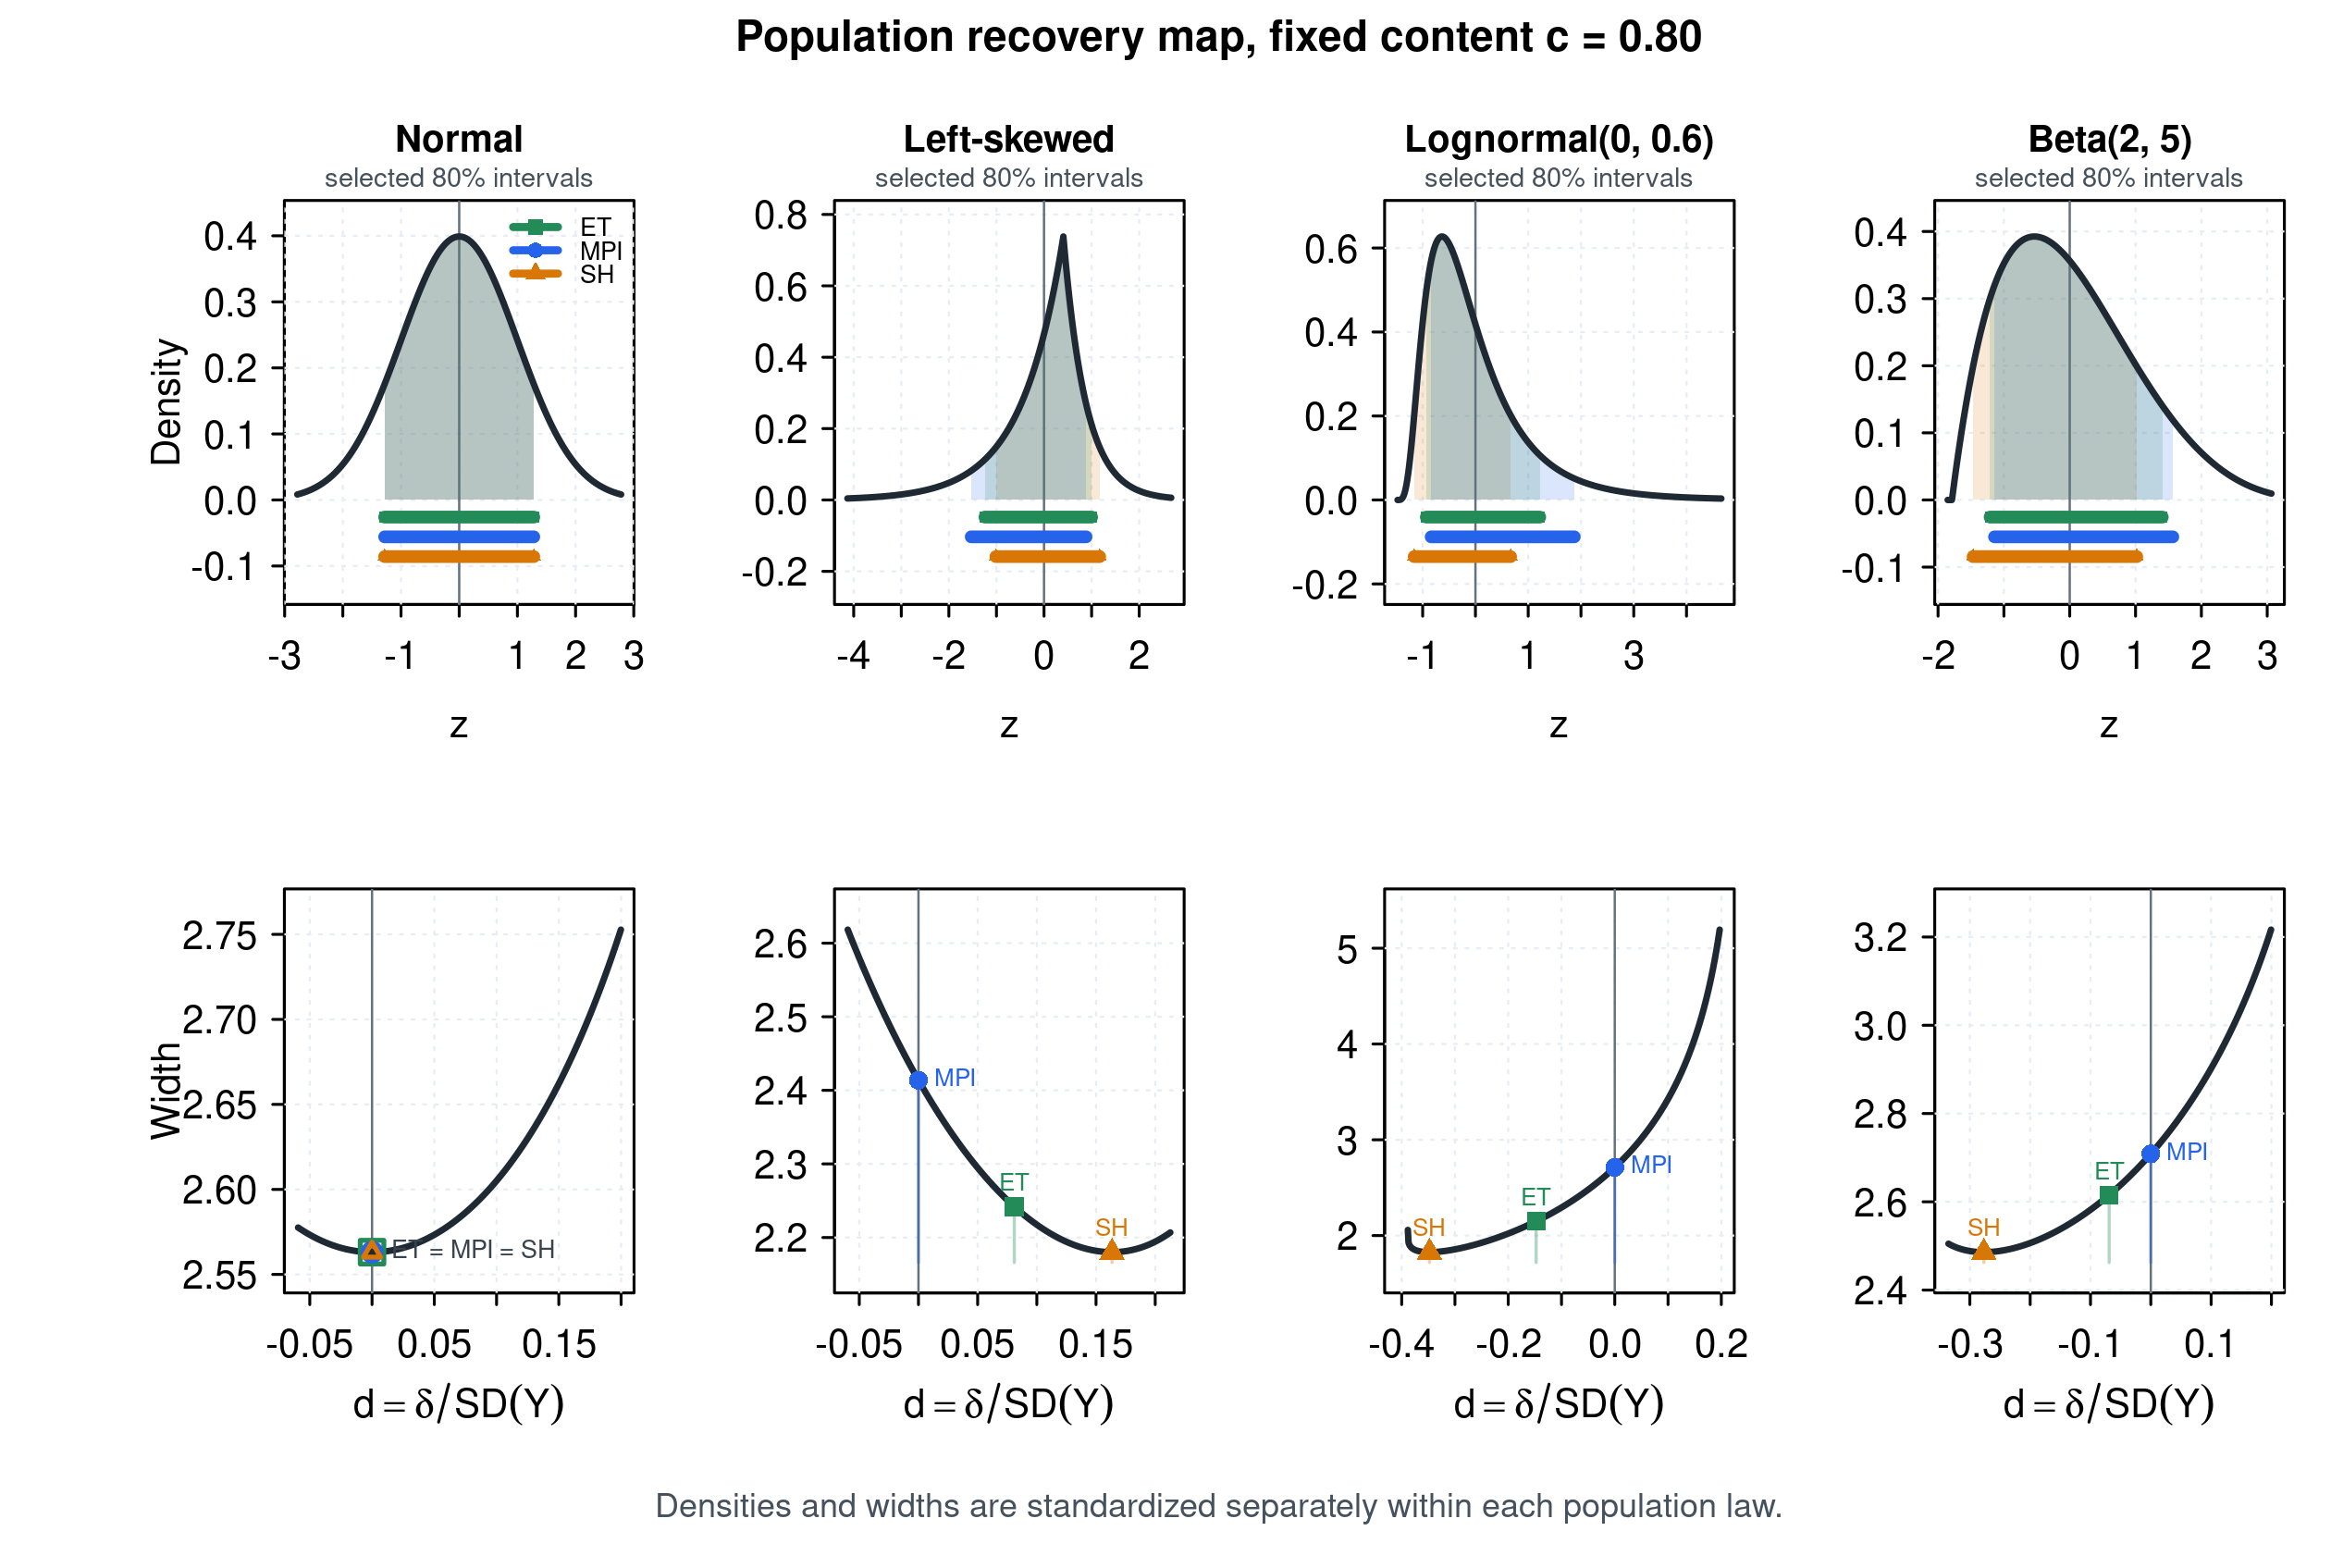
\includegraphics[width=\textwidth]{figures/ch05-mti/generated/figS01_cross_distribution_recovery.png}
\caption{\textbf{Population recovery tilts across symmetric and skewed
distributions.}
Every interval has content \(c=0.80\). Targets are computed on each raw
population law and then displayed after mean/standard-deviation
standardization. The top row shows standardized densities with equal-tailed
  (ET), MPI, and shortest-contiguous (SH) intervals; the bottom row
  shows the standardized width profile along the MTI family. In the
Normal reference case the three targets coincide at
\(\delta/\operatorname{SD}(Y)=0\). Under skewness, ET and SH generally require
  nonzero, distribution-specific recovery tilts, while MPI remains the
zero-tilt retained-mean-balance target. The deterministic display is a
population map for external target specification.}
\label{rqr2026:fig:mean-tilt-map}
\end{figure}

For initialization and external tilt selection, the same identities suggest a
simple first-order approximation. Let \(\gamma_1\) denote standardized
skewness and set
\[
q_c=\Phi^{-1}\{(1+c)/2\},\qquad K_c=q_c\phi(q_c)/c.
\]
A Cornish--Fisher expansion around a standardized Normal law
\citep{rqr-CornishFisher1937} gives the
shortest-oriented and equal-tailed standardized tilt approximations
\[
d_{\mathrm{SH}}^{\mathrm{CF}}=-\gamma_1K_c,\qquad
d_{\mathrm{ET}}^{\mathrm{CF}}=\frac{1}{3}d_{\mathrm{SH}}^{\mathrm{CF}},
\qquad d=\delta/\operatorname{SD}(Y).
\]
These formulas are not new interval targets; they are local skewness-based
approximations to the population recovery tilts. Right skewness gives a
negative shortest-oriented tilt, while left skewness gives a positive tilt.
They supply simple, interpretable starting values for tilt exploration, not
automatic shortest-interval estimators. Figure~\ref{rqr2026:fig:mean-tilt-cf-anchors}
places the two approximations on the exact population tilt path using true
population skewness rather than a sample estimate.

\begin{figure}[H]
\centering
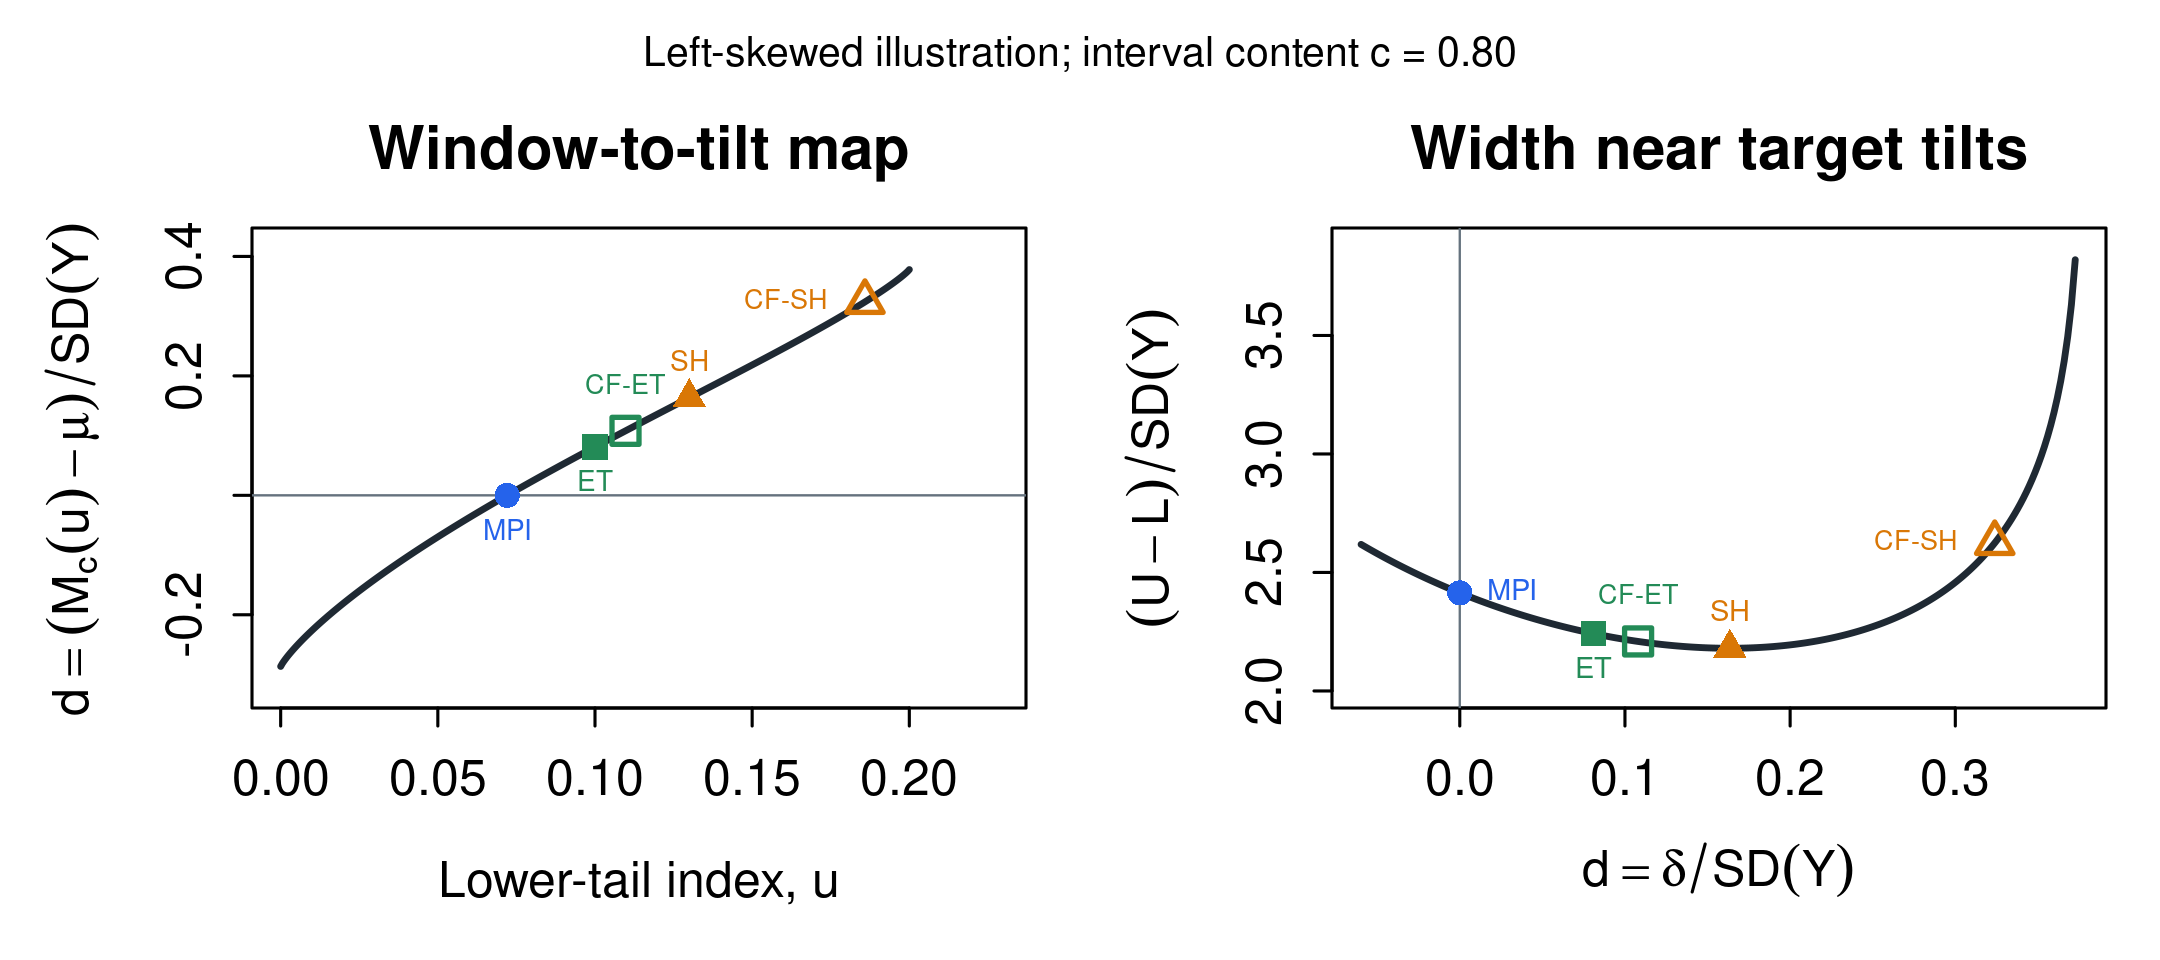
\includegraphics[width=\textwidth]{figures/ch05-mti/generated/fig03_mean_tilt_cf_anchors.png}
\caption{\textbf{Cornish--Fisher recovery-tilt approximation.}
For content \(c=0.80\), the solid curves are the population window-to-tilt
map and width profile from the left-skewed illustration. Filled markers are
the exact population MPI, ET, and SH tilts. Open markers are the first-order
Cornish--Fisher approximations computed from true population skewness. The display
diagnoses a population approximation for initialization and external
tilt selection. Data-driven tilt estimation, MCMC evidence, and response prediction
are separate empirical tasks.}
\label{rqr2026:fig:mean-tilt-cf-anchors}
\end{figure}

\begin{table}[H]
\centering
\caption{\textbf{Population accuracy of first-order Cornish--Fisher recovery-tilt approximations.} Each row uses a known population law, content $c=0.80$, and true skewness $\gamma_1$. Population and CF columns report standardized recovery tilts $d=\delta/\operatorname{SD}(Y)$; $|e|$ is their absolute gap. Gamma arguments are shape and scale, lognormal arguments are meanlog and sdlog, and the exponential law has unit rate. $^{\dagger}$ denotes an SH population value at the lower support boundary. This is a deterministic population calculation, not MCMC, tilt-selection, or response-prediction evidence.}
\label{rqr2026:tab:mean-tilt-cf-mini-study}
\TableStyle
\begin{tabular}{@{}l@{\hspace{0.8em}}rrrrrrr@{}}
\toprule
Distribution & $\gamma_1$ & \multicolumn{3}{c}{Equal-tailed} & \multicolumn{3}{c}{Shortest-contiguous} \\
\cmidrule(lr){3-5} \cmidrule(l){6-8}
& & Population $d$ & CF $d$ & $|e|$ & Population $d$ & CF $d$ & $|e|$ \\
\midrule
Normal & 0.000 & 0.000 & 0.000 & 0.000 & 0.000 & 0.000 & 0.000 \\
Gamma(16, 0.25) & 0.500 & -0.047 & -0.047 & 0.000 & -0.140 & -0.141 & 0.001 \\
Gamma(4, 1) & 1.000 & -0.092 & -0.094 & 0.002 & -0.273 & -0.281 & 0.008 \\
Lognormal(0, 0.5) & 1.750 & -0.128 & -0.164 & 0.036 & -0.323 & -0.492 & 0.169 \\
Exponential$^{\dagger}$ & 2.000 & -0.169 & -0.187 & 0.018 & -0.402 & -0.562 & 0.160 \\
Beta(2, 5) & 0.596 & -0.069 & -0.056 & 0.013 & -0.277 & -0.168 & 0.109 \\
Beta(5, 2) & -0.596 & 0.069 & 0.056 & 0.013 & 0.277 & 0.168 & 0.109 \\
\bottomrule
\end{tabular}
\end{table}


Table~\ref{rqr2026:tab:mean-tilt-cf-mini-study} shows why the approximation should
remain an approximation rather than a target definition. It is exact at symmetry and
close for the near-Normal Gamma laws. Its errors are larger for lognormal and
bounded Beta shapes and for the exponential law, whose shortest interval is a
support-boundary solution. The reflected Beta rows verify the expected sign
reversal but also show that skewness alone does not determine approximation
accuracy. Across these examples the ET approximation is more accurate than the
SH approximation, but that comparison is descriptive rather than a general
ordering.
The numerical summaries therefore report moment shape,
probability-window boundary behavior, and bootstrap sensitivity whenever a
sample plug-in approximation is constructed.

The recovery tilts above are population quantities. A universal tilt does not
recover the same interval functional across distributions, and conditional
recovery generally requires a covariate-dependent \(\delta(x)\). The tilt is
therefore fixed or selected by a separate validation rule; sampling
it as an ordinary parameter would mix distinct interval targets. The target is
equivariant under positive affine changes of response scale when \(\delta\)
and the fixed learning rate are transformed accordingly, but it is not
invariant to arbitrary monotone response transformations. Generalized-Bayes
computations with nonzero tilt require the target content, tilt, learning rate,
and prior class to be specified before the loss update is evaluated. Other
prior, learning-rate, and model classes require separate propriety arguments and
validation. Data-driven tilt selection likewise requires an independent
selection rule before empirical claims are made.

The population score equations do not by themselves establish propriety of a
finite-sample generalized posterior under an arbitrary root prior. With a
fixed learning rate, a finite design, and proper Gaussian root priors, the tilt
is linear in the root parameters and the Gaussian tails make the generalized
posterior proper. This argument covers ridge regression with proper Gaussian
root priors. Heavier-tailed shrinkage priors and dependent root processes
require separate propriety analyses before nonzero tilt is considered.

\section{Empirical balance and fixed-target computation}
\label{rqr2026:sec:static-theory-statements}

The population theory above concerns unrestricted fixed-content intervals. A
finite sample adds two separate questions: what the fitted interval balances on
the training data, and how a fixed-target MTI calculation is used after a
content and tilt have been chosen.

\paragraph{Training-sample balance.}
Fitted endpoints depend on the observations, and the empirical MPI/MTI loss is
nonsmooth when an observation lies on a root. The finite-sample score identity is
therefore fractional. For intercept-only MTI with fixed \(\delta\), let
\((\widehat a,\widehat b)\), \(\widehat a<\widehat b\), be an interior
subgradient-stationary empirical solution. Then there exist allocations
\(\widehat q_i\in[0,1]\), equal to one for observations strictly inside the
fitted interval, zero for observations strictly outside it, and fractional only
at fitted roots, such that
\[
\sum_{i=1}^n \widehat q_i=nc,
\qquad
\sum_{i=1}^n \widehat q_i y_i
=nc(\overline y+\delta).
\]
Thus the fitted training interval has exact fractional content and exact
fractional retained-mean balance in its empirical estimating equations.
These identities concern the unpenalized criterion. Gaussian root penalties
contribute additional terms to the estimating equations used in computation;
Section~\ref{app:mti-profile-computation} gives the corresponding penalized identities.
Population content requires a probability argument beyond this score identity.
In the iid intercept-only case, the Dvoretzky--Kiefer--Wolfowitz inequality gives
a conservative high-probability population-content bound
\citep{rqr-Massart1990DKW}; Section~\ref{app:mti-proofs} records the explicit
bound and its limited interpretation.

\paragraph{Fixed-target generalized-Bayes computation.}
For a fixed fitted content \(q\), tilt \(\delta\), and learning rate
\(\omega_{\mathrm R}\), an MTI generalized posterior updates a prior over
interval roots through the cumulative loss,
\[
\pi_{q,\delta}(\theta\mid D_n)
\propto
\exp\{-\omega_{\mathrm R}L_{q,\delta,n}(\theta)\}\pi_0(\theta).
\]
In the intercept-only tolerance validation, \(\theta=(a,b)\) and ordered
endpoints are obtained by sorting the two raw roots. This distribution is a
loss-based generalized posterior for a fixed interval target. Response
prediction would require a separate response-distribution model. The tilt
\(\delta\) is fixed within each candidate fit; the profiled selection rule
described below chooses among these fits.

For the intercept-only calculation, the two roots have independent
\(\Normal(0,\lambda^{-1})\) priors. Writing the endpoints as \(m-h,m+h\)
reduces minimization in \(h^2\) to an empirical quantile of squared distances
from \(m\). The resulting midpoint criterion is strongly convex when
\(\lambda>0\). We minimize this scalar profile and recover the endpoints,
checking the objective gap against a relative tolerance of \(10^{-8}\).
The validation uses \(\omega_{\mathrm R}=1\) and \(\lambda=10^{-4}\).
Section~\ref{app:mti-profile-computation} gives the profile identity and its
objective-gap check. Broader Gibbs, ECM, regression, basis-expansion, and
time-varying endpoint calculations are summarized in
Section~\ref{app:mti-extensions}.

\paragraph{Direct content-probability check.}
MTI uses a response-distribution posterior probability to check the content
of each fitted candidate. For a fixed interval \(I\), a direct
Dirichlet-process posterior for
\(F\) gives an exact Beta law for \(F(I)\) conditional on the observed sample
\citep{rqr-Ferguson1973DP}. This check is used to select eligible MTI
candidates during the fitted-content and tilt search. Its probability threshold
is chosen in a separate calibration run. The resulting tolerance performance
is then assessed on independent simulation samples.

\section{Calibrated MTI tolerance intervals}
\label{rqr2026:sec:mti-tolerance}

The preceding theory fixes population content and interval placement. A
tolerance interval adds a repeated-sampling requirement. For iid continuous
univariate observations, the target statement is
\[
\Pr_F^n\{C_F(\widehat T_n)\ge c\}\ge 1-\alpha,\qquad
C_F([L,U])=F(U)-F(L),
\]
where \(\widehat T_n\) is a data-dependent interval. Six quantities must be
kept distinct. The required population content is \(c\), and the tolerance
confidence is \(1-\alpha\). The fitted MTI content is \(q\in(c,1)\),
which can vary continuously and need not equal a sample fraction. The MTI
placement tilt is \(\delta\), and the
generalized-Bayes learning rate is \(\omega_{\mathrm R}\). When a separate
response-distribution model for \(F\) is used, \(\gamma\) denotes a posterior
content-probability threshold for eligible intervals. The learning rate controls
the loss update, and the posterior threshold controls candidate eligibility.
Tolerance confidence concerns the repeated-sampling behavior of the complete
selection rule.

\paragraph{Fitted-content and tilt search.}
For a training sample, construct candidate pairs
\(\{(q_j,\delta_j):j=1,\ldots,J\}\). For each pair, the profile calculation
computes endpoint estimates
\(\widehat I_j=[\widehat a_j,\widehat b_j]\) using the fixed-target update
in Section~\ref{rqr2026:sec:static-theory-statements}. A direct DP posterior for \(F\)
then gives
\[
P_j=\Pr\{F(\widehat b_j)-F(\widehat a_j)\ge c\mid D_n\}.
\]
The selected interval is
\[
\widehat T_n=\widehat I_{\widehat j},\qquad
\widehat j=\argmin_{j:\,P_j\ge\gamma}
\{\widehat b_j-\widehat a_j\},
\]
where the minimization is restricted to finite fitted intervals. Ties are
resolved by smaller fitted content, proximity to the empirical shortest-window
tilt, lower endpoint, and candidate order, in that order. If no candidate is
eligible, the procedure records that no interval was produced. No substitute
interval is inserted into the comparison.

The initial content grid uses the retained fraction \(k/n\) from uniform-scan
calibration as a reference, with fixed offsets and additional contents near
one. Its refinement accounts for the effective observation mass
\(s=nq-\lambda/\omega_{\mathrm R}\) in the radius profile. Within the range of
the initial grid, we add one interior content for each unrepresented interval
\(r-1<s<r\), where \(r\) is an order-statistic rank. At each content,
the tilt candidates include zero, the fractional shortest-window retained-mean
offset, and seven equally spaced positions across the empirical admissible
tilt range. Fractional contents between \((n-1)/n\) and one allow the loss to
remain below the boundary \(q=1\), including when the reference uses the full
sample range. All grid rules are fixed before calibration.

\paragraph{Calibration and interpretation.}
For each \((n,c,1-\alpha)\) setting, independent development samples determine
a finite menu of posterior probability cutoffs. Each cutoff is assessed on
24,000 new samples from each of the eight calibration distributions. We select
the smallest cutoff for which every distribution returns all intervals and
has a simultaneous one-sided exact binomial lower bound for content attainment
of at least \(1-\alpha\). The bound accounts for the number of distributions,
settings, and assessed cutoffs. A follow-up specified before fresh sampling resolves two settings
using more finely spaced development cutoffs, while preserving seven earlier
choices and controlling the combined Monte Carlo error at \(0.05\).
Section~\ref{app:mti-calibration} gives the allocation and selected cutoffs. This calibration
concerns the complete interval-selection rule on the finite distributional
panel. All choices are fixed before independent validation.

Theorems~\ref{rqr2026:thm:quantile-window}--\ref{rqr2026:thm:profiled-mean-tilt} identify
the population MTI family and its admissible tilt coordinate. The exact DP
Beta law describes posterior content under the specified response-distribution
model. Neither result by itself supplies a distribution-free tolerance theorem
for the fitted-content and tilt selection rule. Its observed content-attainment
rates in Section~\ref{rqr2026:sec:evaluation} provide empirical repeated-sampling
evidence for the prespecified design. The shortest-candidate property is
restricted to the evaluated grid of numerical fits. Selected-target endpoint
uncertainty and regression-family tolerance calibration require additional
results.

\paragraph{Shortest-path continuation.}
The population shortest-window path gives useful continuation geometry for
moving across contents and explains the width cost of increasing fitted
content. Suppose that the density is
differentiable and strictly unimodal,
and that the shortest window
\(I_q=[L_q,U_q]=[Q(u_q),Q(u_q+q)]\) is unique and interior over a range of
\(q\). Equal endpoint densities then satisfy
\[
f(L_q)=f(U_q)=\lambda_q.
\]
Writing \(a_q=f'(L_q)>0\) and \(b_q=f'(U_q)<0\), formal differentiation of
the content and equal-density equations gives
\[
L_q'=\frac{b_q}{\lambda_q(a_q-b_q)}<0,
\qquad
U_q'=\frac{a_q}{\lambda_q(a_q-b_q)}>0.
\]
Thus the first-order shares of added probability assigned to the left and
right boundaries are
\[
p_L(q)=\frac{-b_q}{a_q-b_q},\qquad
p_R(q)=\frac{a_q}{a_q-b_q},\qquad
p_L(q)+p_R(q)=1.
\]
Only under local symmetry are the two shares equal to one half. The width
satisfies
\[
W_{\mathrm{SH}}'(q)=\frac{1}{\lambda_q},
\qquad
W_{\mathrm{SH}}''(q)
=-\frac{a_qb_q}{\lambda_q^3(a_q-b_q)}>0.
\]
Hence additional content becomes increasingly expensive as the endpoints move
into lower-density regions. If
\(m_q=q^{-1}\int_{u_q}^{u_q+q}Q(s)\,ds
=\mu+\delta_{\mathrm{SH}}(q)\), then
\[
\delta_{\mathrm{SH}}'(q)
=\frac{p_L(q)L_q+p_R(q)U_q-m_q}{q}.
\]
These derivatives describe the population path under the stated interior
conditions. The implemented MTI procedure evaluates its finite grid directly;
it does not require these derivatives. Boundary and nonunique shortest
intervals require separate treatment.

\section{Validation design}
\label{rqr2026:sec:evaluation}

The validation study assesses population content attainment and interval width
under repeated sampling. The population MTI identities identify the target
family, while the simulation study evaluates the complete fitted-content and
tilt selection rule.

The tolerance study evaluates the selected MTI rule on samples independent
of its calibration, following simulation-study reporting principles
\citep{rqr-MorrisWhiteCrowther2019Simulation}. It uses iid continuous samples from
eight centered and scaled simulation distributions. Gaussian and Student \(t_3\)
samples serve as symmetric reference distributions. The asymmetric simulation
distributions are exponential,
asymmetric Laplace with \(\tau=0.10\), a two-piece Normal law with scale ratio
\(1{:}12\), Beta\((1,8)\), Gamma\((0.5,1)\), and log-normal with log-scale
standard deviation \(1.25\). This panel is intentionally skewed toward
asymmetric laws to examine interval placement when equal-tail or full-range
behavior can be inefficient.
Multimodal cases are excluded because none of the reported methods is designed
to recover disconnected high-density regions.
The primary simulation design fixes tolerance confidence at \(0.95\) and uses
1000 replications per method, simulation distribution, and feasible cell.
MTI, Young--Mathew, and Wilks use the same samples in every replication.
These validation samples are independent of both threshold development and
calibration assessment, allowing paired comparisons of attainment and width.
The feasible cells are \(n=50,c=0.90\), \(n=100,c\in\{0.90,0.95\}\), and
\(n\in\{500,1000\},c\in\{0.90,0.95,0.99\}\).

The small-sample restriction is structural. For a two-sided distribution-free
interval, even the full sample range reaches content \(c\) with confidence
\(0.95\) only when
\[
  1-n(1-c)c^{n-1}-c^n \ge 0.95 .
\]
For intervals contained in the sample range, the corresponding minimum sample
sizes are \(46\), \(93\), and \(473\) for
\(c=0.90\), \(0.95\), and \(0.99\), respectively. Thus
\(n=50,c=0.95\) and \(n=100,c=0.99\) are excluded from the confirmatory
comparison because the sample-bounded order-statistic comparators cannot
support the requested statement in those cells. These thresholds describe the
design's distribution-free reference class; they are not a feasibility theorem
for the model-based MTI rule. The \(c=0.99\) rows begin at \(n=500\), the
nearest rounded sample size above the \(n=473\) threshold.

MTI is the proposed method in the comparison. It uses a calibration rule indexed
by sample size and requested content. Within each cell, the rule fixes a direct
Dirichlet-process content-probability check from an independent calibration run, profiles
fixed-target MTI endpoint fits over fitted content and retained-mean tilt,
and keeps the shortest candidate satisfying the content-probability check.
The cutoff is selected by the simultaneous calibration bounds in
Section~\ref{rqr2026:sec:mti-tolerance}; the scan provides an initial fitted-content
reference. Tolerance performance is assessed on the fresh validation samples.
Young--Mathew interpolation
\citep{rqr-YoungMathew2014NonparametricTolerance} and Wilks min--max intervals
\citep{rqr-Wilks1941ToleranceLimits,rqr-Wilks1942StatisticalPrediction} provide the
classical order-statistic comparators. The primary metric is the
content-attainment rate: the Monte Carlo estimate of
\(\Pr_F^n\{C_F(\widehat T_n)\ge c\}\), where
\(C_F([L,U])=F(U)-F(L)\). For each replication, this content check uses the
known simulation distribution rather than the fraction of sampled observations
inside the produced interval. If a method produced no interval in a replication,
that replication would be counted as nonattainment. Widths are reported as
distribution-level empirical 2.5\%--97.5\% ranges, avoiding width averages
across distributions with different scales and tail behavior.
Figure~\ref{rqr2026:fig:tolerance-validation-width-ranges} also marks the population
shortest content-\(c\) interval for each simulation law. This benchmark uses
the known distribution and serves as a lower width reference rather than as a
sample-based tolerance procedure.

\begin{table}[!htbp]
\centering
\caption{\textbf{Independent-sample tolerance validation.} Results are shown by
feasible sample-size/content cell and method. Each row summarizes the range
across eight simulation distributions at tolerance confidence \(0.95\). All three
reported methods produced an interval in every replication in this run.}
\label{rqr2026:tab:tolerance-validation-primary}
\TableStyle
\begin{tabular}{@{}l@{\hspace{0.75em}}l@{\hspace{0.75em}}r@{}}
\toprule
Design & Method & Content-attainment range (\%)\\
\midrule
\(n=50,c=0.90\) & MTI & 96.1--98.0 \\
 & Young--Mathew & 95.4--96.9 \\
 & Wilks & 96.1--98.0 \\
\addlinespace[0.25em]
\(n=100,c=0.90\) & MTI & 95.5--98.3 \\
 & Young--Mathew & 95.1--97.9 \\
 & Wilks & 100.0--100.0 \\
\addlinespace[0.25em]
\(n=100,c=0.95\) & MTI & 95.6--97.3 \\
 & Young--Mathew & 95.1--96.9 \\
 & Wilks & 95.6--97.3 \\
\addlinespace[0.25em]
\(n=500,c=0.90\) & MTI & 96.0--99.1 \\
 & Young--Mathew & 94.5--96.6 \\
 & Wilks & 100.0--100.0 \\
\addlinespace[0.25em]
\(n=500,c=0.95\) & MTI & 97.1--98.9 \\
 & Young--Mathew & 94.6--98.3 \\
 & Wilks & 100.0--100.0 \\
\addlinespace[0.25em]
\(n=500,c=0.99\) & MTI & 95.1--97.3 \\
 & Young--Mathew & 95.0--97.2 \\
 & Wilks & 95.1--97.3 \\
\addlinespace[0.25em]
\(n=1000,c=0.90\) & MTI & 95.7--99.3 \\
 & Young--Mathew & 94.1--95.6 \\
 & Wilks & 100.0--100.0 \\
\addlinespace[0.25em]
\(n=1000,c=0.95\) & MTI & 95.9--99.1 \\
 & Young--Mathew & 94.7--96.6 \\
 & Wilks & 100.0--100.0 \\
\addlinespace[0.25em]
\(n=1000,c=0.99\) & MTI & 97.5--99.3 \\
 & Young--Mathew & 94.5--97.9 \\
 & Wilks & 99.9--100.0 \\
\addlinespace[0.25em]
\bottomrule
\end{tabular}

\end{table}

\begin{figure}[!htbp]
\centering
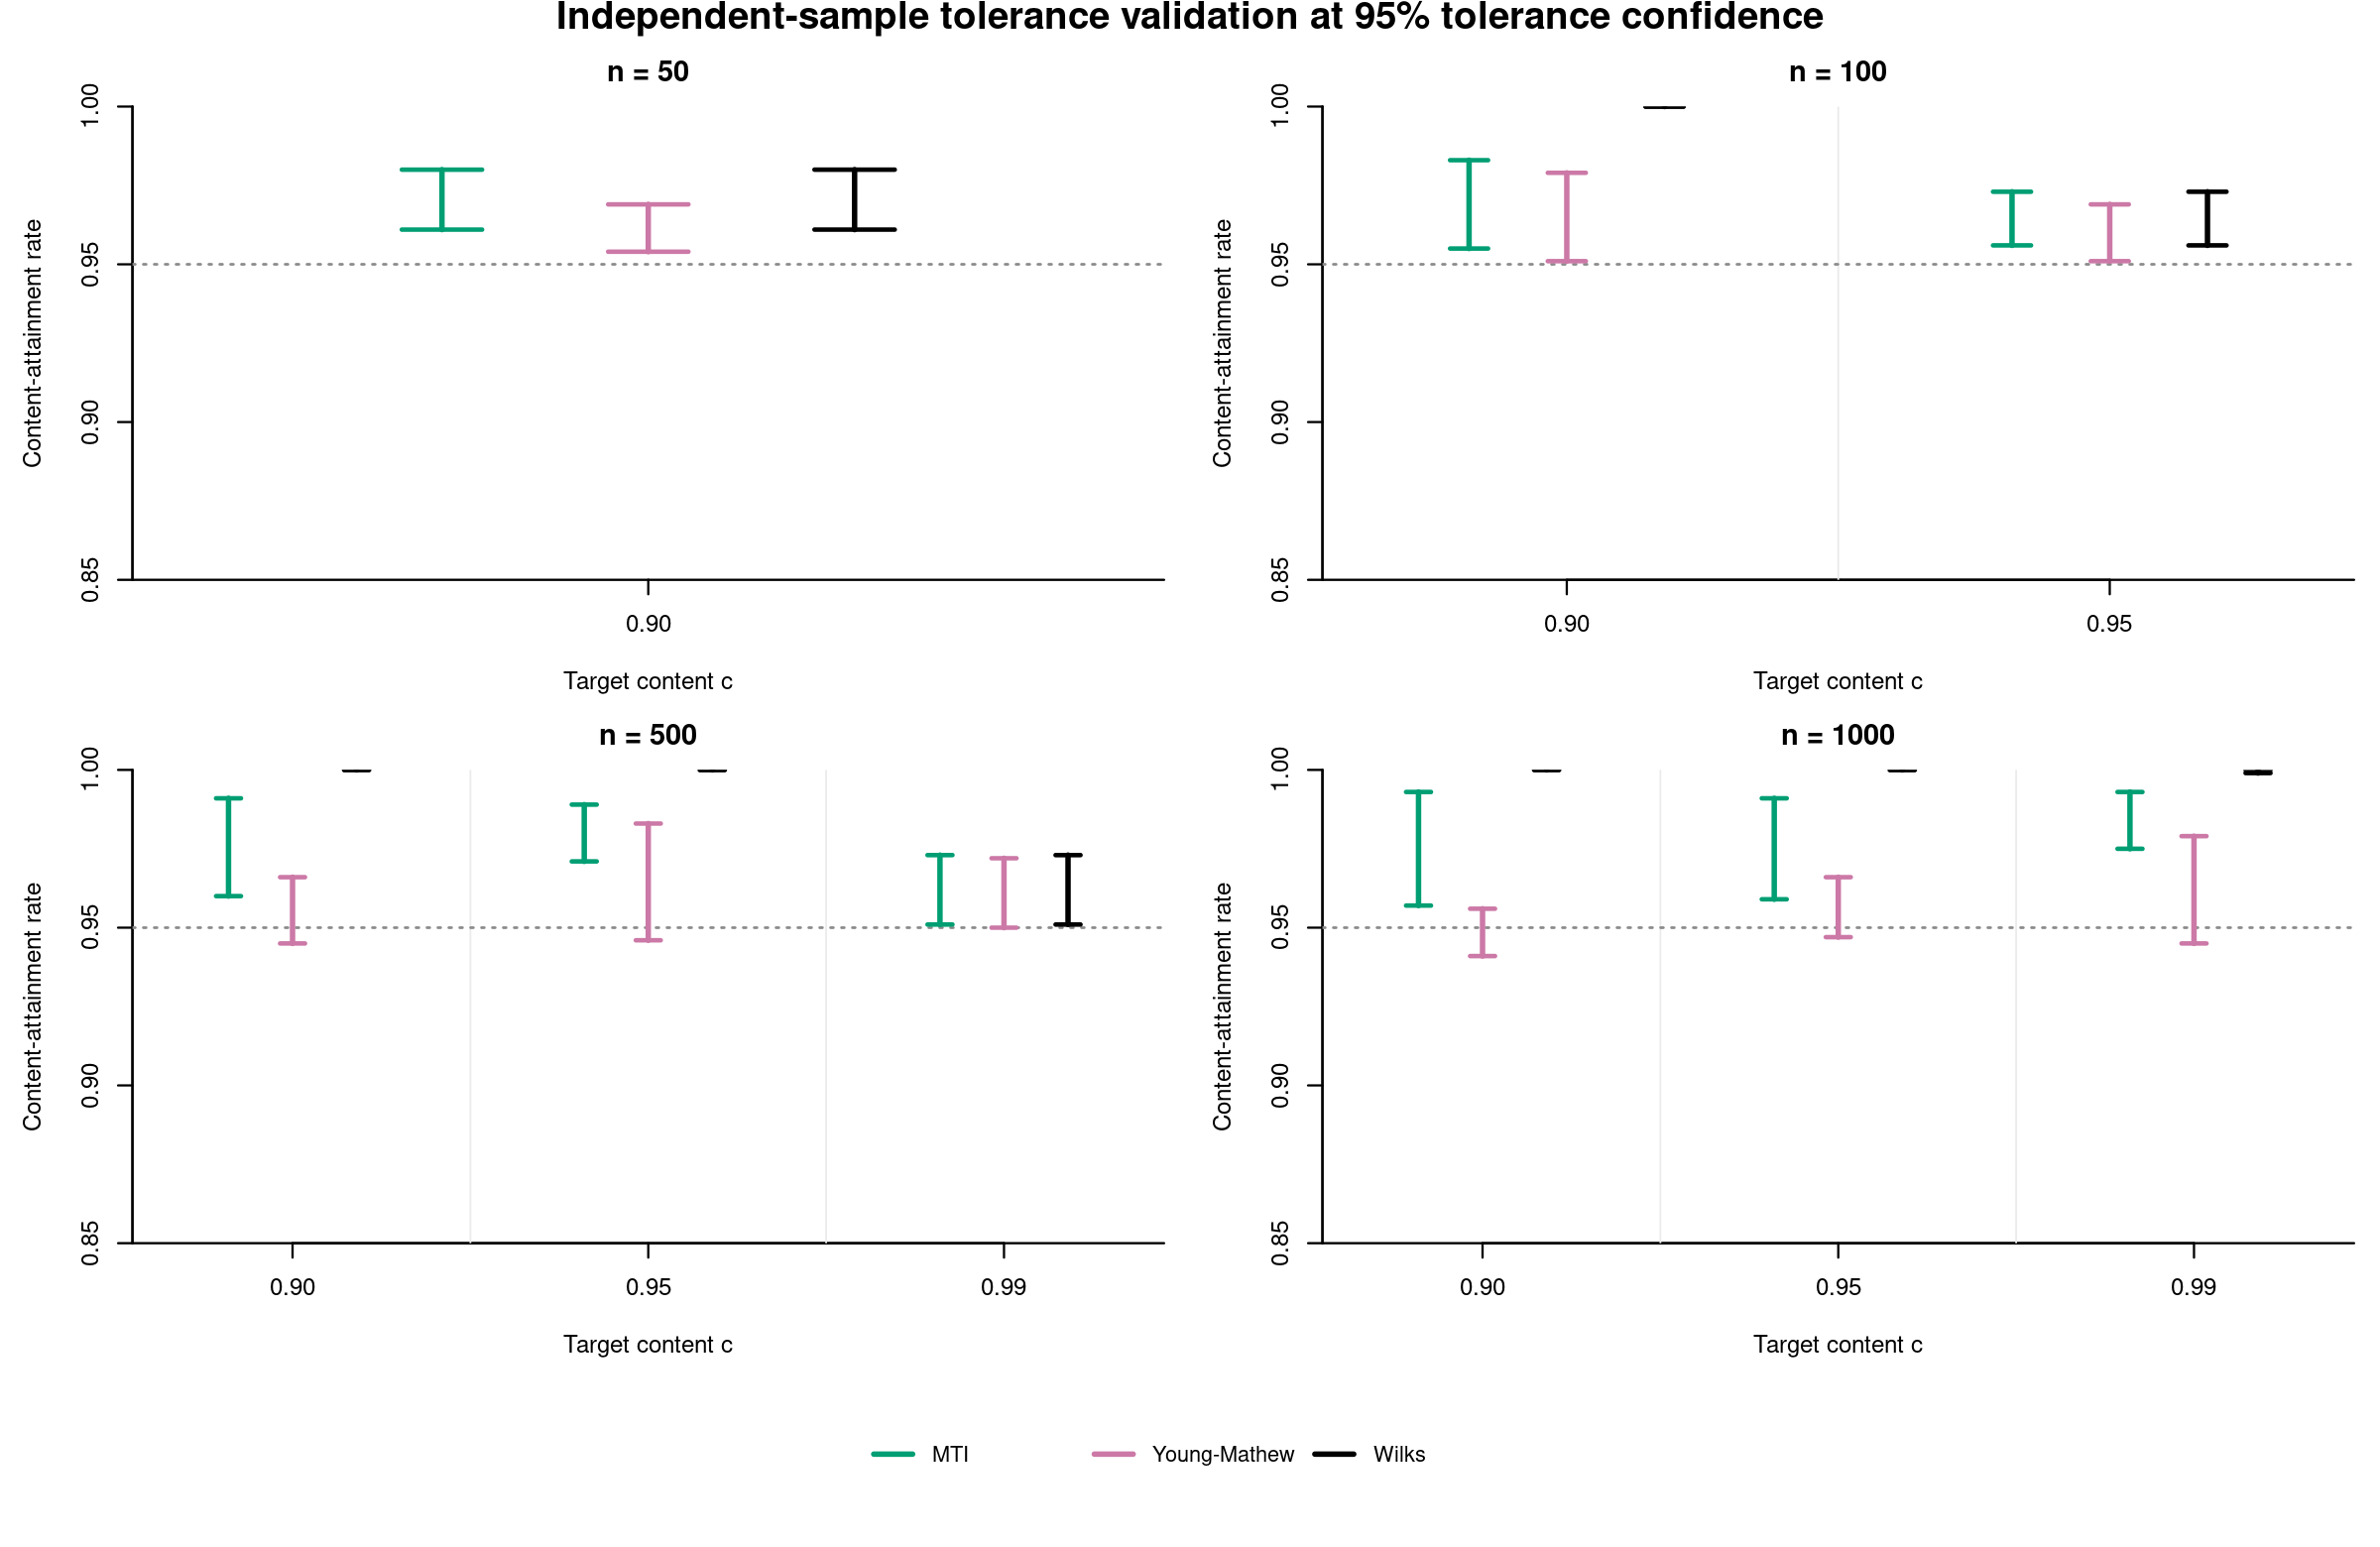
\includegraphics[width=\textwidth]{figures/ch05-mti/generated/fig04_tolerance_validation_primary.png}
\caption{\textbf{Content-attainment by sample size and target content.}
Intervals not produced are counted as nonattainment.
Vertical intervals in the content-attainment panels show the range across
distributional scenarios, and the axis is zoomed to \(0.85\)--\(1.00\).
Dashed reference lines mark nominal tolerance confidence \(0.95\).}
\label{rqr2026:fig:tolerance-validation-primary}
\end{figure}

\begin{figure}[!htbp]
\centering
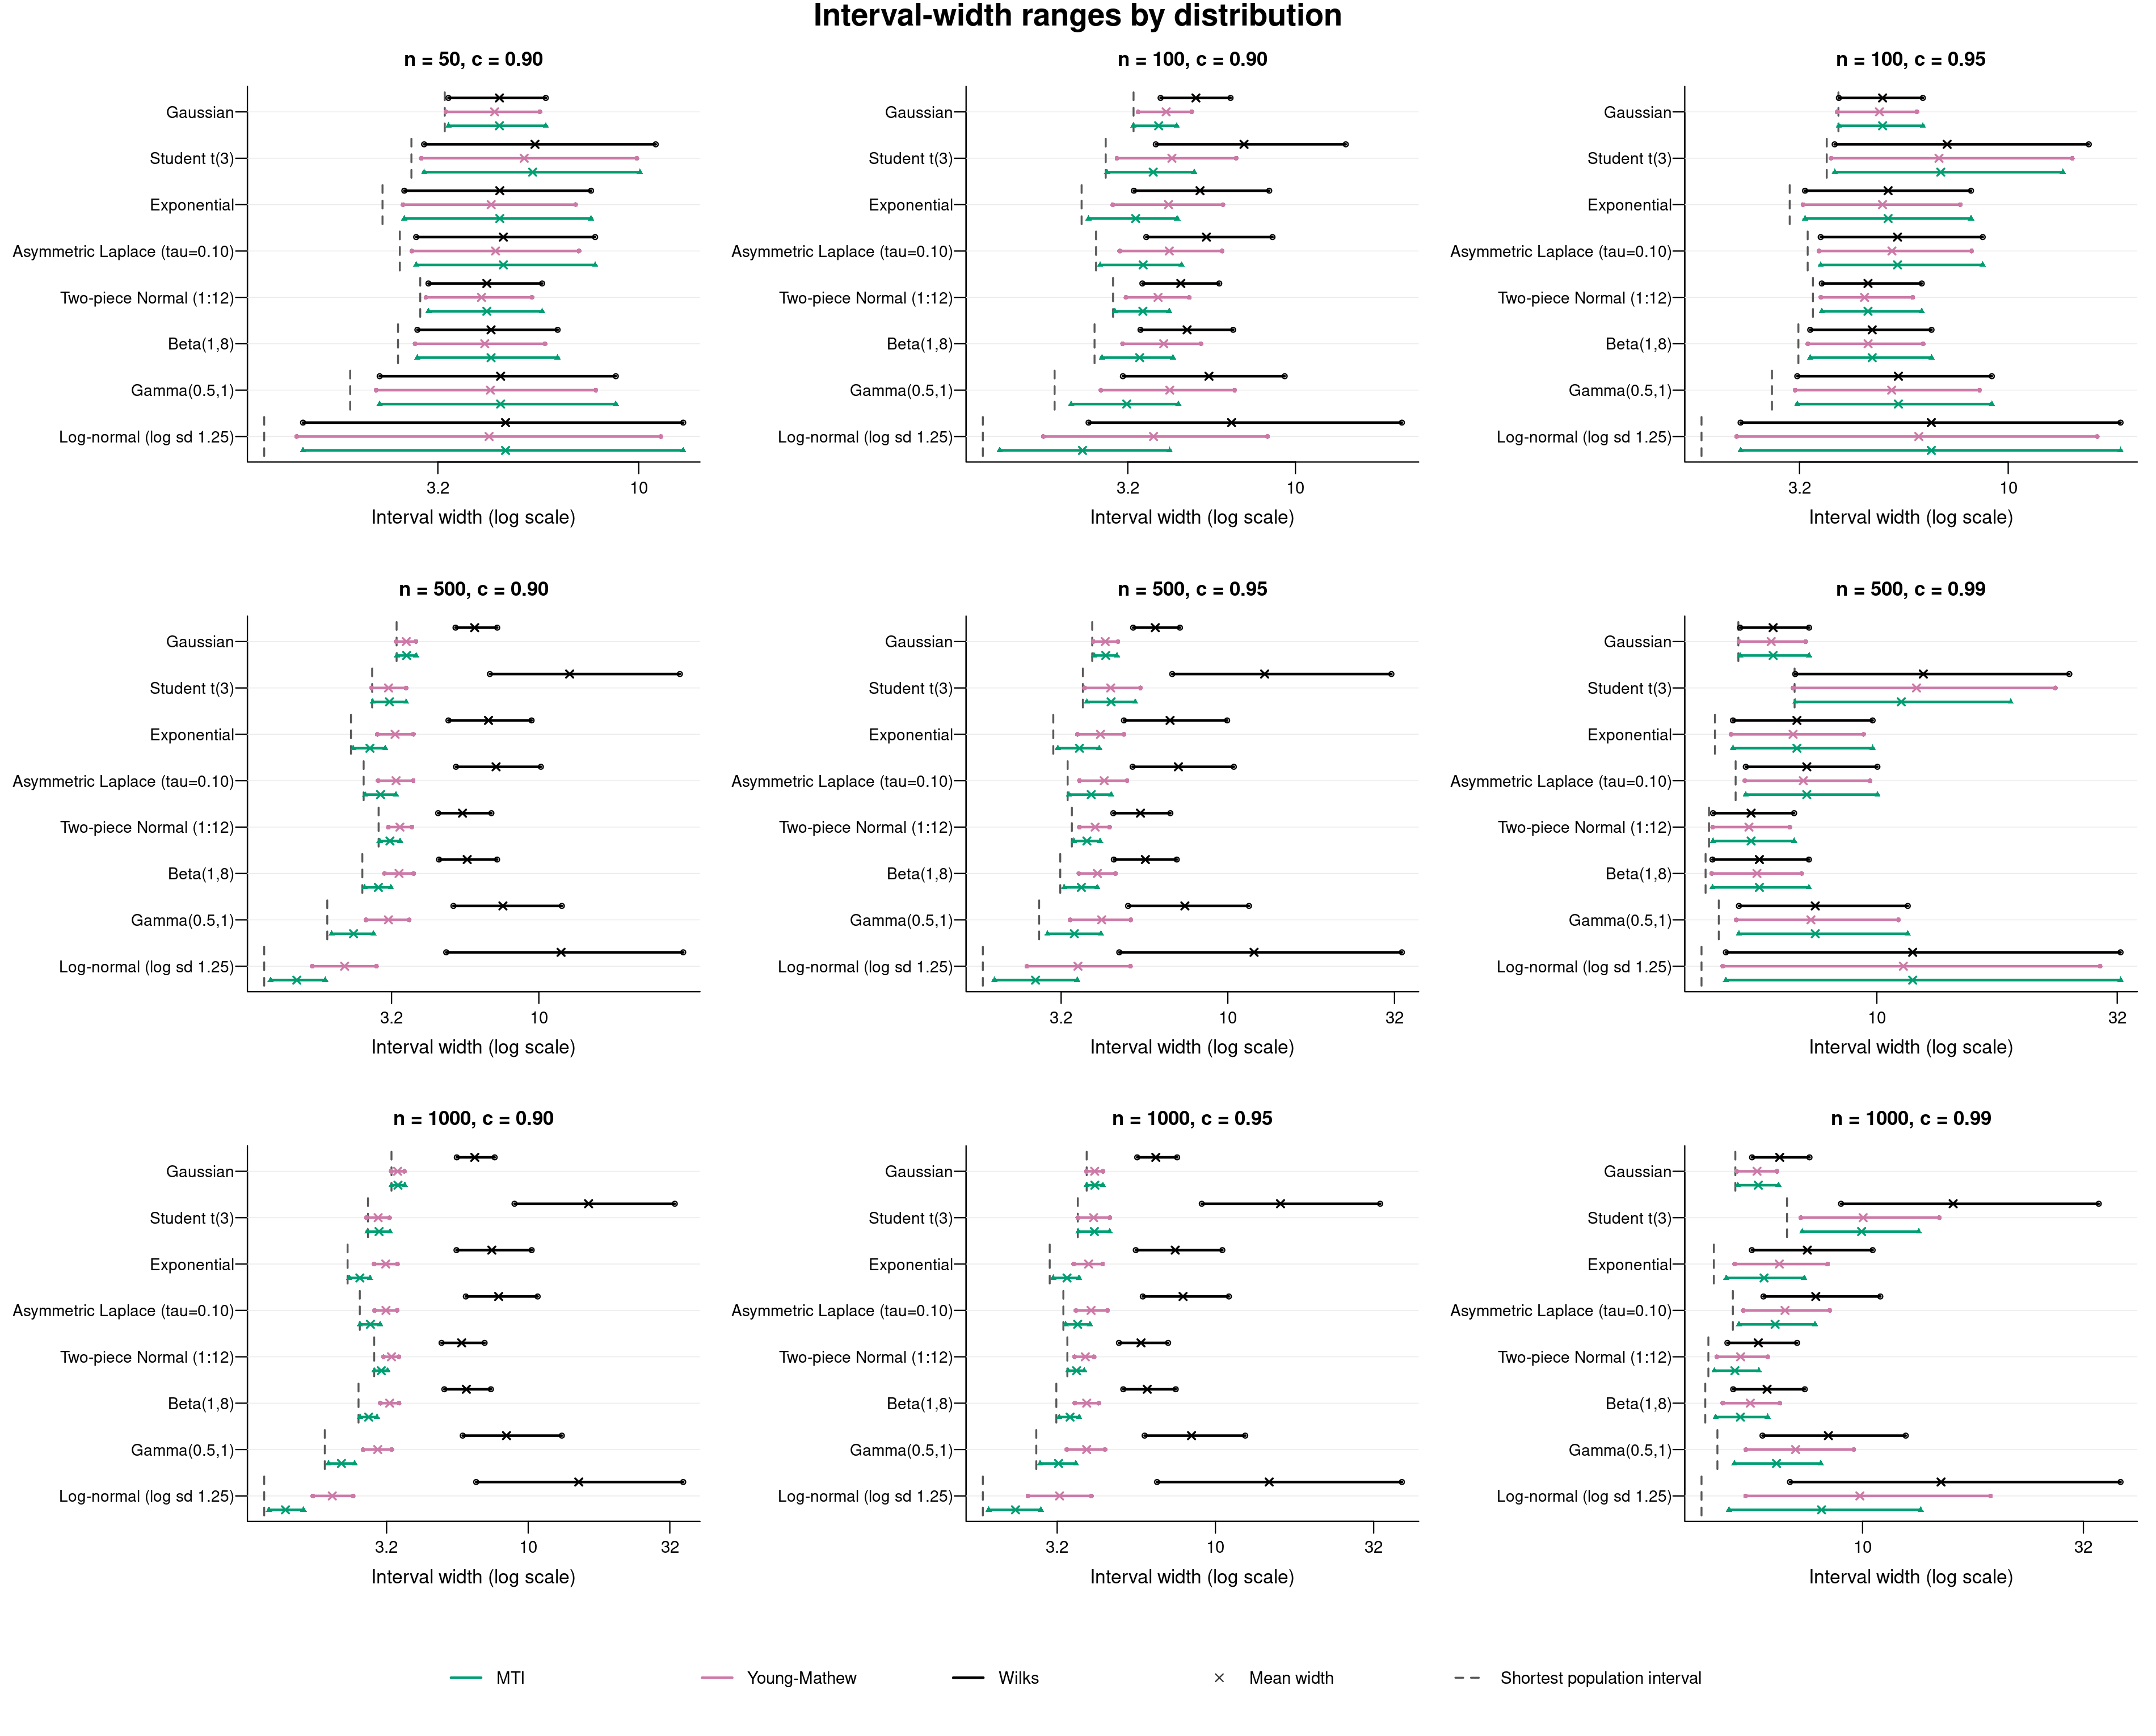
\includegraphics[width=\textwidth]{figures/ch05-mti/generated/fig05_tolerance_validation_width_ranges.png}
\caption{\textbf{Interval-width ranges by distribution.} Horizontal intervals show empirical
2.5\%--97.5\% ranges of interval lengths within each distribution,
sample-size/content cell, and method. Crosses mark the mean interval width
across the 1000 replications for that method. Dashed gray markers show the corresponding
population shortest content-\(c\) interval widths under the known simulation
laws. The horizontal axis is logarithmic to display light-tailed, heavy-tailed,
and strongly skewed cases in one figure; the values remain raw interval
lengths.}
\label{rqr2026:fig:tolerance-validation-width-ranges}
\end{figure}

In the completed run, MTI content attainment ranges from 95.1\% to 99.3\%
across distribution-level cells, compared with
94.1\% to 98.3\% for Young--Mathew, and 95.1\% to 100.0\% for Wilks.
Figures~\ref{rqr2026:fig:tolerance-validation-primary}
and~\ref{rqr2026:fig:tolerance-validation-width-ranges} show the same comparison without
pooling widths across distributional scenarios. In the independent validation
run, the selected MTI rule has observed content attainment above the nominal
tolerance confidence in all 72 distribution-level cells. The closest
independent validation cells remain near the nominal boundary, so this evidence
should be read as repeated-sampling validation of the selected MTI rule
rather than as a distribution-free finite-sample guarantee. Of the 72
simultaneous validation confidence intervals, 38 have lower bounds above
\(0.95\) and 34 include \(0.95\); none has an upper bound below it.
The larger calibration assessment has lower bounds above \(0.95\) in all
72 cases.

MTI has smaller mean width than Young--Mathew in 40 of 72 cases and greater
mean width in 32. For each of the six asymmetric distributions it is shorter
in six of nine designs. At \(n=100,c=0.90\), mean reductions range from
5.0\% to 38.6\% across distributions. At \(n=50,c=0.90\) and
\(n=100,c=0.95\), Young--Mathew is shorter in every distribution.
Near the sample-range boundary, MTI often returns the Wilks interval:
their endpoints agree in 99.0\%, 98.2\%, and 94.7\% of samples at
\((n,c)=(50,0.90),(100,0.95),(500,0.99)\), respectively.
These cases illustrate the limited observed width gain near that boundary.

Section~\ref{app:mti-calibration} records the selected MTI policy,
scan-reference counts, and full-range feasibility thresholds used to choose
the simulation design. The distribution-level results are summarized above
through their ranges and simultaneous uncertainty statements.
The excluded small-sample cells fall outside the region where a sample-bounded
two-sided distribution-free tolerance statement can be supported at confidence \(0.95\).
Other variants are kept outside the primary comparison.

\section{Pharmaceutical batch application}
\label{rqr2026:sec:pharma-application}
\newcommand{\PharmaBatches}{187}
\newcommand{\PharmaRawBatches}{1005}
\newcommand{\PharmaRawFields}{55}
\newcommand{\PharmaProductCode}{23}
\newcommand{\PharmaTrain}{100}
\newcommand{\PharmaHeldout}{87}
\newcommand{\PharmaSplits}{1000}
\newcommand{\PharmaContent}{0.90}
\newcommand{\PharmaConfidence}{0.95}
\newcommand{\PharmaScreen}{0.984112}
\newcommand{\PharmaRetained}{98}
\newcommand{\PharmaGroupedSplits}{250}
\newcommand{\PharmaObjectiveTolerance}{10^{-8}}
\newcommand{\PharmaMaxObjectiveGap}{9.94e-14}
\newcommand{\PharmaTensileMtiWidth}{0.514}
\newcommand{\PharmaTensileMtiLower}{1.101}
\newcommand{\PharmaTensileMtiUpper}{1.618}
\newcommand{\PharmaTensileMtiContent}{95.4}
\newcommand{\PharmaTensileMtiAttainment}{88.0}
\newcommand{\PharmaTensileMtiLowerOmitted}{1.1}
\newcommand{\PharmaTensileMtiUpperOmitted}{2.3}
\newcommand{\PharmaTensileYmWidth}{0.533}
\newcommand{\PharmaTensileYmLower}{1.133}
\newcommand{\PharmaTensileYmUpper}{1.690}
\newcommand{\PharmaTensileYmContent}{95.4}
\newcommand{\PharmaTensileYmAttainment}{91.9}
\newcommand{\PharmaTensileYmLowerOmitted}{2.3}
\newcommand{\PharmaTensileYmUpperOmitted}{1.1}
\newcommand{\PharmaTensileWilksWidth}{0.665}
\newcommand{\PharmaTensileWilksLower}{1.040}
\newcommand{\PharmaTensileWilksUpper}{1.748}
\newcommand{\PharmaTensileWilksContent}{98.9}
\newcommand{\PharmaTensileWilksAttainment}{99.3}
\newcommand{\PharmaTensileWilksLowerOmitted}{0.0}
\newcommand{\PharmaTensileWilksUpperOmitted}{0.0}
\newcommand{\PharmaTensileConverged}{1000}
\newcommand{\PharmaTensileReturned}{1000}
\newcommand{\PharmaTensileConvergenceRate}{100.0}
\newcommand{\PharmaTensileSkewness}{0.44}
\newcommand{\PharmaTensileRepresentative}{665}
\newcommand{\PharmaTensilePairedYmWidthDifference}{-0.014}
\newcommand{\PharmaTensileForwardContent}{96.6}
\newcommand{\PharmaTensileReverseContent}{89.7}
\newcommand{\PharmaRsdMtiWidth}{1.690}
\newcommand{\PharmaRsdMtiLower}{0.610}
\newcommand{\PharmaRsdMtiUpper}{2.300}
\newcommand{\PharmaRsdMtiContent}{95.4}
\newcommand{\PharmaRsdMtiAttainment}{90.6}
\newcommand{\PharmaRsdMtiLowerOmitted}{1.1}
\newcommand{\PharmaRsdMtiUpperOmitted}{3.4}
\newcommand{\PharmaRsdYmWidth}{2.262}
\newcommand{\PharmaRsdYmLower}{0.700}
\newcommand{\PharmaRsdYmUpper}{2.970}
\newcommand{\PharmaRsdYmContent}{95.4}
\newcommand{\PharmaRsdYmAttainment}{87.9}
\newcommand{\PharmaRsdYmLowerOmitted}{3.4}
\newcommand{\PharmaRsdYmUpperOmitted}{1.1}
\newcommand{\PharmaRsdWilksWidth}{3.400}
\newcommand{\PharmaRsdWilksLower}{0.600}
\newcommand{\PharmaRsdWilksUpper}{4.050}
\newcommand{\PharmaRsdWilksContent}{98.9}
\newcommand{\PharmaRsdWilksAttainment}{99.3}
\newcommand{\PharmaRsdWilksLowerOmitted}{0.0}
\newcommand{\PharmaRsdWilksUpperOmitted}{0.0}
\newcommand{\PharmaRsdConverged}{1000}
\newcommand{\PharmaRsdReturned}{1000}
\newcommand{\PharmaRsdConvergenceRate}{100.0}
\newcommand{\PharmaRsdSkewness}{3.00}
\newcommand{\PharmaRsdRepresentative}{364}
\newcommand{\PharmaRsdPairedYmWidthDifference}{-0.447}
\newcommand{\PharmaRsdForwardContent}{85.1}
\newcommand{\PharmaRsdReverseContent}{98.9}

\newcommand{\PharmaCampaigns}{28}
\newcommand{\PharmaFctHardnessQuestions}{36}
\newcommand{\PharmaCoreHardnessQuestions}{55}
\newcommand{\PharmaRandomSharedHeldout}{85}
\newcommand{\PharmaCampaignDisjointMonths}{63}
\newcommand{\PharmaCampaignDisjointApiShared}{58}
\newcommand{\PharmaPreparedGroupPartitions}{250}
\newcommand{\PharmaCampaignTensileContent}{92.0}
\newcommand{\PharmaCampaignTensileAttainment}{71.4}
\newcommand{\PharmaCampaignRsdContent}{92.0}
\newcommand{\PharmaCampaignRsdAttainment}{55.6}


Pharmaceutical batch records illustrate interval placement for a reported
derived measurement. We compare the proposed MTI procedure with
the Young--Mathew and Wilks benchmarks using the public manufacturing data of
\citet{rqr-ZagarMihelic2022PharmaManufacturing} and the associated
\texttt{Laboratory.csv} file \citep{rqr-ZagarMihelic2021LaboratoryCsv}.

Each observation represents one batch. Product code \PharmaProductCode{}
provides \PharmaBatches{} batches with a common recorded strength and batch
size. The response is the reported film-coated-tablet tensile metric,
computed from batch summaries of hardness and tablet dimensions.
Its sample skewness is \PharmaTensileSkewness{}, making it a
moderately skewed example alongside the more asymmetric simulation laws.
The public file does not resolve the physical unit of this derived measure
or supply product-specific acceptance criteria. In
\PharmaFctHardnessQuestions{} batches, average hardness exceeds its recorded
maximum. The summaries' measurement windows and units require clarification
before that ordering can be interpreted. We retain the source values and
use the derived metric to describe historical batch variation; its physical
interpretation remains provisional.

The primary analysis uses \PharmaSplits{} paired random splits, each with
\PharmaTrain{} training and \PharmaHeldout{} held-out batches. Every method
uses the same observations within a split, and both responses considered here
use the same partition definitions. The requested population content is
\(c=\PharmaContent\), with nominal tolerance confidence
\(\PharmaConfidence\). The MTI cutoff is the simulation-calibrated value
\(\gamma=\PharmaScreen\) for \(n=100,c=0.90\). Candidate construction,
priors, and numerical settings are applied unchanged to the historical
partitions, without tuning on held-out outcomes. Young--Mathew and Wilks use the conventions in
Section~\ref{rqr2026:sec:evaluation}. All intervals are closed, so held-out values
equal to an endpoint count as included.

Held-out empirical content is the fraction of withheld batches inside the
fitted interval. Lower- and upper-tail omission are the fractions below and
above its endpoints. These summaries describe the finite dataset. Overlapping
splits do not provide independent sampling replications, and recorded ties
and possible batch dependence limit an iid continuous interpretation.
The controlled repeated-sampling tolerance evidence remains the simulation
study in Section~\ref{rqr2026:sec:evaluation}.
The associated process records identify \PharmaCampaigns{} production
campaigns \citep{rqr-ZagarMihelic2021Process}. Every random partition shares
campaigns between training and evaluation; a median
\PharmaRandomSharedHeldout{} of \PharmaHeldout{} withheld batches belong to
campaigns represented in training. The random-split results consequently
describe variation within this historical production setting.

\begin{table}[!htbp]
\centering
\caption{\textbf{Reported pharmaceutical tensile metric.} Intervals are
fit on \PharmaTrain{} batches and evaluated on \PharmaHeldout{} withheld
batches over \PharmaSplits{} paired random splits. These splits reuse one
finite dataset and are not independent sampling replications. Bracketed ranges
are empirical 2.5\%--97.5\% partition quantiles. The source metric has
unresolved measurement definitions. Lower and upper endpoints are summarized
separately. Held-out \(\ge c\) gives the percentage of all splits with
held-out empirical content at least \(c\); returned intervals and tail
omissions are reported separately.}
\label{rqr2026:tab:pharma-application-primary}
\TableStyle
\begin{tabularx}{\textwidth}{@{}lrr>{\raggedright\arraybackslash}X>{\raggedright\arraybackslash}X@{}}
\toprule
Method & Splits & Returned (\%) & Median lower/upper & Width median [95\% range]\\
\midrule
MTI (proposed) & 1000 & 100.0 & 1.101 / 1.618 & 0.514 [0.422, 0.577] \\
Young--Mathew (benchmark) & 1000 & 100.0 & 1.133 / 1.690 & 0.533 [0.445, 0.593] \\
Wilks (benchmark) & 1000 & 100.0 & 1.040 / 1.748 & 0.665 [0.552, 0.708] \\
\bottomrule
\end{tabularx}
\par\smallskip
\begin{tabularx}{\textwidth}{@{}l>{\raggedright\arraybackslash}Xrr@{}}
\toprule
Method & Held-out content median [95\% range] (\%) & Held-out $\ge c$ (\%) & Omitted below/above (\%)\\
\midrule
MTI & 95.4 [86.2, 98.9] & 88.0 & 1.1 / 2.3 \\
Young--Mathew & 95.4 [87.7, 100.0] & 91.9 & 2.3 / 1.1 \\
Wilks & 98.9 [93.1, 100.0] & 99.3 & 0.0 / 0.0 \\
\bottomrule
\end{tabularx}

\end{table}

\begin{figure}[!htbp]
\centering
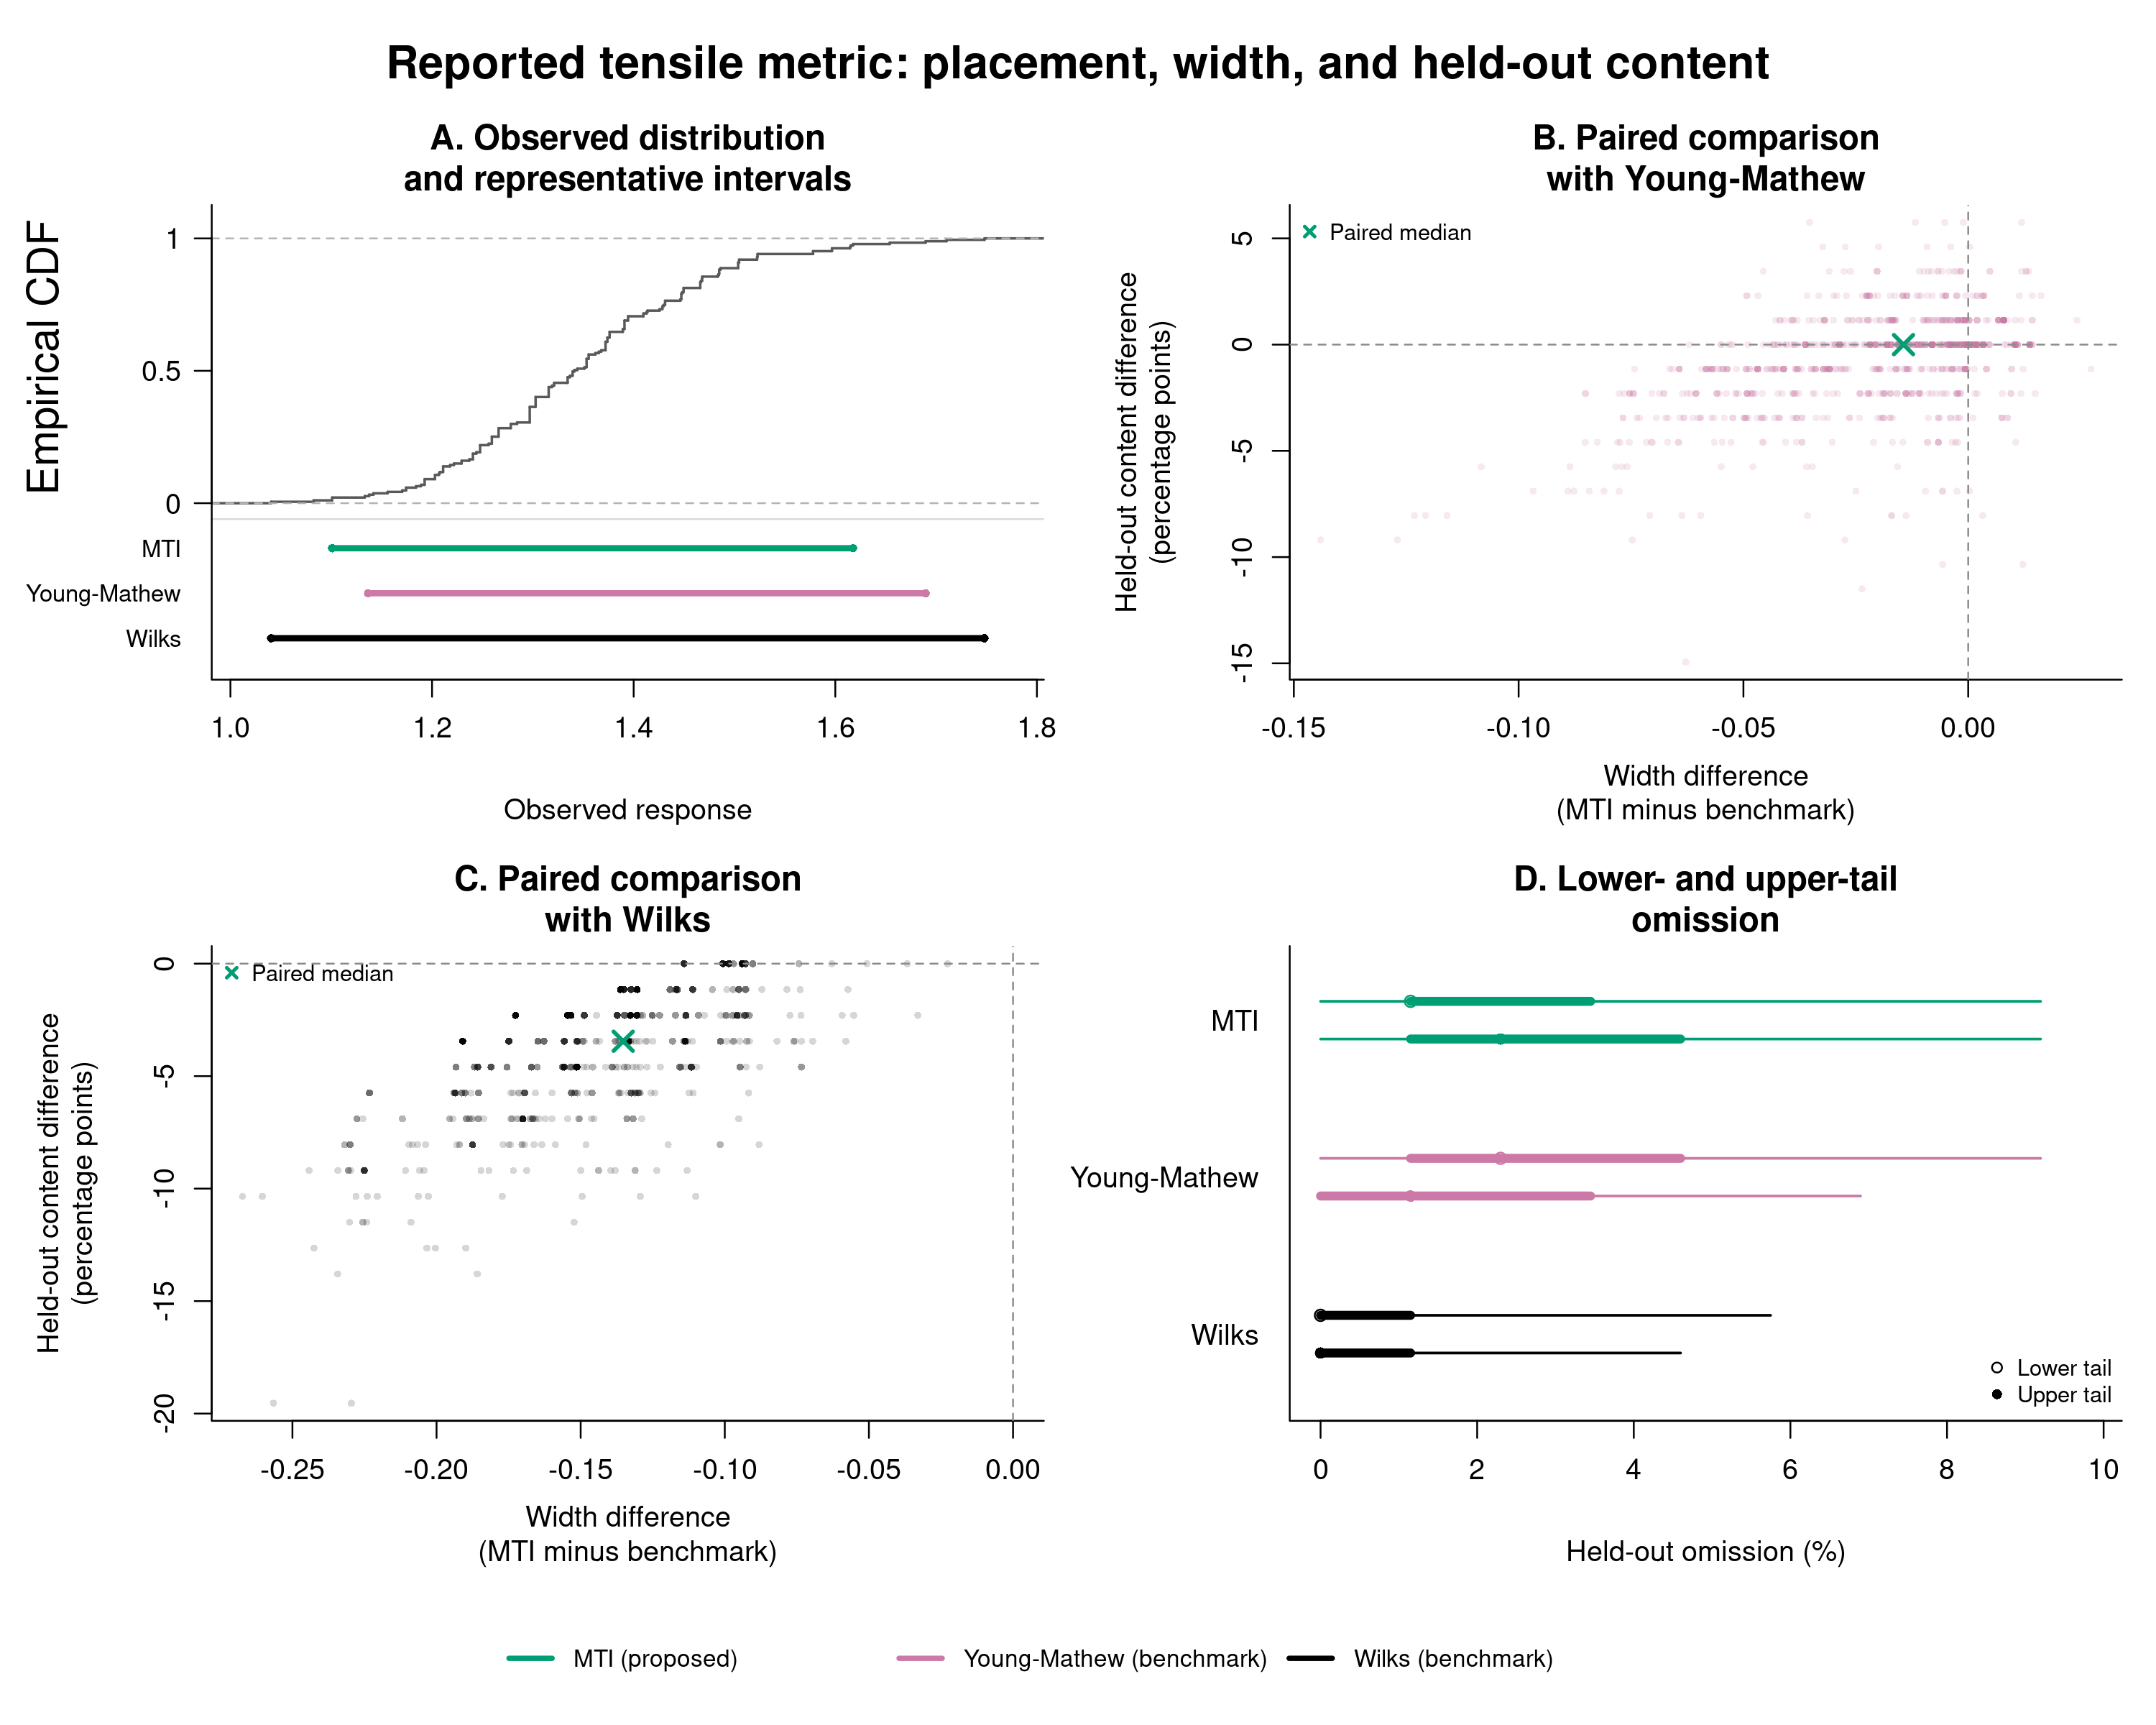
\includegraphics[width=\textwidth]{figures/ch05-mti/generated/fig06_pharma_application_tensile_intervals.png}
\caption{\textbf{Interval placement and held-out comparisons for the reported
tensile metric.} Panel A shows the empirical distribution of all \PharmaBatches{}
batches and actual fitted intervals from split
\PharmaTensileRepresentative{}, selected by the prespecified median-distance
rule. The interval rows below the CDF are positioned for display. Panels B
and C show paired width and held-out-content differences, MTI minus each
benchmark, with crosses marking paired medians. Panel D shows median tail
omission, interquartile ranges (thick segments), and empirical 95\% ranges
(thin segments) across random splits.}
\label{rqr2026:fig:pharma-application-primary}
\end{figure}

MTI has median width \PharmaTensileMtiWidth{}, compared with
\PharmaTensileYmWidth{} for Young--Mathew and \PharmaTensileWilksWidth{} for
Wilks. The median paired width difference against Young--Mathew is
\PharmaTensilePairedYmWidthDifference{}. Median held-out empirical content is
\PharmaTensileMtiContent\% for MTI and \PharmaTensileYmContent\% for
Young--Mathew. Their tail allocations differ: MTI omits median fractions
\PharmaTensileMtiLowerOmitted\% below and
\PharmaTensileMtiUpperOmitted\% above, whereas Young--Mathew allocates
\PharmaTensileYmLowerOmitted\% and \PharmaTensileYmUpperOmitted\%,
respectively. Width and empirical content should therefore be read together
with endpoint placement.

Section~\ref{app:mti-application-sensitivity} examines forward and reverse recorded-order partitions and
\PharmaGroupedSplits{} unique partitions that keep either production months
or active pharmaceutical ingredient (API) batches intact. All retain the same
training size. For example, reverse recorded order gives MTI held-out content
of \PharmaTensileReverseContent\%, illustrating sensitivity to the partition.
The profile objective-gap criterion is met in
\PharmaTensileConverged{} of \PharmaTensileReturned{} returned tensile-metric
fits. Numerical diagnostics and tablet-core weight sensitivity are reported in
Section~\ref{app:mti-application-sensitivity}. The tablet-core weight relative standard
deviation (RSD) example illustrates stronger asymmetry; its
upper-adverse interpretation would favor a one-sided
upper tolerance limit for a direct quality-control decision.
\section{Proposed regression and dynamic endpoint extensions}
\label{mti:sec:extensions}

The fixed-target MTI loss also defines endpoint functions when interval
placement varies with predictors or time. These extensions address estimation
of a chosen content--tilt target; they do not automatically produce a response
distribution or a tolerance guarantee. For observations
\(D_n=\{(x_i,y_i):i=1,\ldots,n\}\), let the two raw endpoint functions be
\(\eta_1(x;\theta_1)\) and \(\eta_2(x;\theta_2)\). Given fixed content \(c\),
tilt \(\delta\), learning rate \(\omega_{\mathrm R}\), and prior
\(\pi_0\), the generalized posterior is
\begin{equation}
\pi(\theta_1,\theta_2\mid D_n)
\propto
\exp\{-\omega_{\mathrm R}L_{c,\delta,n}(\theta_1,\theta_2)\}
\pi_0(\theta_1,\theta_2).
\label{mti:eq:generalized-posterior}
\end{equation}
The learning rate controls the scale of the loss update and is distinct from
content, tilt, and any response-distribution parameter.

For static linear endpoint regression, the raw roots are
\(\eta_j(x)=x^\top\beta_j\), \(j=1,2\). Because the loss is unchanged when the
root labels are exchanged, interpretation is based on sorted fitted endpoints
\[
L(x)=\min\{\eta_1(x),\eta_2(x)\},\qquad
U(x)=\max\{\eta_1(x),\eta_2(x)\}.
\]
Equivalently, midpoint and signed-gap coefficients
\(\beta_m=(\beta_1+\beta_2)/2\) and
\(\beta_s=(\beta_2-\beta_1)/2\) give
\(L(x)=x^\top\beta_m-|x^\top\beta_s|\) and
\(U(x)=x^\top\beta_m+|x^\top\beta_s|\).
A coefficient-wise lower/upper interpretation is justified only over a design
region where the root ordering does not change.

A normal--exponential representation of the product-residual check loss gives
generalized-inverse-Gaussian latent-scale updates and a Gaussian conditional
update for either root given the other. It supports Gibbs computation and a
deterministic ECM mode calculation under proper Gaussian priors. The
representation augments the loss factor in
Equation~\eqref{mti:eq:generalized-posterior}; it is not a sampling density for
\(Y\). Section~\ref{app:mti-extensions} records the latent-scale law, Gaussian
canonical parameters, fixed-tilt shift, shrinkage construction for the
zero-tilt case, and numerical safeguards.

Deterministic basis expansions use the same equations after replacing the
design rows by fixed basis vectors. Time-varying endpoints instead use two
root-specific state trajectories,
\[
\eta_{jt}=f_t^\top\theta_{jt},\qquad
\theta_{jt}=G_t\theta_{j,t-1}+\varepsilon_{jt},\qquad j=1,2,
\]
with Gaussian state innovations. Conditional on one complete root path and the
latent scales, the other path has a linear Gaussian representation, motivating
alternating forward-filtering backward-sampling updates. The conditional
derivation is given in Section~\ref{app:mti-extensions}.

These constructions remain proposed methods. The derivations have no matched
implementation, simulation study, or application.
Endpoint regression should be evaluated using recovery of known endpoint
functions, held-out MTI loss, empirical content, and width. A dynamic analysis
must additionally state its basis or state prior and the rule used to select
discount factors. Repeated-sampling tolerance claims require a separate,
action-matched calibration study; predictive claims require a specified
response-distribution model. Neither is supplied by the generalized posterior
alone.

\section{Discussion}
\label{rqr2026:sec:discussion}

Probability content determines a class of interval placements. Under the stated
population conditions, MPI selects the member whose retained mean equals the
population mean. MTI makes retained-mean balance an explicit coordinate:
\(\delta=0\) returns MPI, while admissible nonzero tilts specify other
contiguous content-\(c\) windows. Equal-tailed and shortest-contiguous
intervals are distribution-specific members of this placement family rather
than universally equivalent targets.

The calibrated procedure uses this family to search for short tolerance
intervals. Fixed-target endpoint estimates are combined with a direct
Dirichlet-process posterior content check, and a separate calibration run fixes
the selection rule before validation. In the independent study, empirical
content attainment exceeds the nominal tolerance confidence in every reported
cell, and MTI has smaller mean width than Young--Mathew in two thirds of the
asymmetric cells. The independent confidence bounds remain inconclusive in 34
of the 72 cases. These findings apply to the frozen procedure and the stated
eight-distribution design. The finite grid, numerical calculation, and
simulation calibration do not establish broader optimality or a
distribution-free theorem.

The separation among target, computation, and tolerance confidence is
essential. MTI identifies the fixed-content interval being estimated. A
generalized posterior describes uncertainty for a fixed loss-defined target.
A response model, such as the Dirichlet-process posterior used for the content
screen, gives model-based content probabilities. The selected tolerance action
is evaluated by repeated-sampling content attainment. A guarantee for that
selected action requires an argument beyond fixed-target posterior computation.

The pharmaceutical analysis has a narrower, descriptive role. It shows how the
precalibrated procedures place endpoints on historical batch measurements and
how held-out content changes with the partition. Overlapping splits, possible
batch dependence, ties, unresolved measurement definitions, and shared
production campaigns restrict its interpretation for future production.

The tolerance evidence is confined to iid continuous univariate simulations,
and boundary tilts can lead to one-sided limits or inactive roots. The proposed
regression and dynamic endpoint models generalize the loss-defined target, not
the validation result. Implementations, numerical diagnostics, simulation
designs, and target-specific calibration are required before empirical
performance or repeated-sampling tolerance behavior can be claimed for those
extensions.

\chapter{Synthesis, limitations and future work}
\label{ch:synthesis}

\section{A target-first synthesis}
\label{sec:synthesis-target-first}

The four research chapters approach distributional inference from different
directions. Chapter~\ref{ch:research-a} makes dynamic quantile methodology
usable through a software implementation and a coherent analysis sequence. Chapter
\ref{ch:research-b} uses that model to correct and synthesize heterogeneous
hydrologic products. Chapter~\ref{ch:research-c} replaces linear state
evolution for the quantile location with fixed nonlinear recurrent features.
Chapter~\ref{ch:research-d} changes the inferential object from pointwise
conditional quantiles to fixed-content interval placement and tolerance
actions. These are linked contributions, but they are not four implementations
of one model.

Table~\ref{tab:synthesis-comparison} compares the projects along the dimensions
that determine their statistical interpretations. The target and update
columns are especially important. Chapters~\ref{ch:research-a}--
\ref{ch:research-c} use AL or exAL likelihood contributions to study
conditional quantiles and, in selected analyses, synthesized future-response
distributions. Chapter~\ref{ch:research-d} uses a residual-product loss to
define interval endpoints and a separate repeated-sampling calibration to
construct a tolerance action. A common latent-variable algebra does not erase
this difference.

\begin{table}[htbp]
\centering
\begingroup
\small
\setlength{\tabcolsep}{3pt}
\renewcommand{\arraystretch}{1.08}
\begin{tabularx}{\textwidth}{@{}p{0.14\textwidth}YYYY@{}}
\toprule
\textbf{Chapter} & \textbf{Primary target} & \textbf{Dependence representation}
& \textbf{Update and computation} & \textbf{Principal evidence} \\
\midrule
2: \pkg{exdqlm} & Dynamic or static conditional quantile; post-fit predictive
synthesis & Linear latent states, transfer components, or static regression &
AL/exAL likelihood; MCMC, LDVB, and ISVB interfaces & Software examples,
diagnostics, held-out scores, and exact version contract \\
3: hydrology & Source-corrected conditional quantiles and a synthesized
future-response distribution & Shared latent quantile process with source-
specific discrepancies and transfer covariates & exAL dynamic model with LDVB
and supporting MCMC algorithms & Five retrospective forecast origins under a
globally specified model; separate 28-day and common 8-day comparisons \\
4: Q--DESN & Single or joint conditional quantiles & Fixed deep-reservoir
features followed by Bayesian regression & AL/exAL working likelihood; MCMC
and model-specific VB--LD & Development-informed known-DGP simulations and
retrospective GloFAS and PriceFM applications \\
5: MTI & Fixed-content interval placement; calibrated empirical tolerance
action & Static endpoints or proposed regression and dynamic endpoint states &
Generalized Bayes for fixed targets; convex profiling and calibrated content
screening & Population results, independent simulation validation, and a
descriptive pharmaceutical application \\
\bottomrule
\end{tabularx}
\endgroup
\caption{Comparison of the four research chapters. The entries identify the
main inferential object and the strongest evidence available; they do not imply
that the validation designs are interchangeable.}
\label{tab:synthesis-comparison}
\end{table}

Three connections emerge from this comparison. First, distributional targets
can be modeled without committing every analysis to a complete parametric
response distribution. The quantile chapters target selected conditional
features, while the MTI chapter begins from the geometry of a fixed-content
interval. Second, temporal structure can enter through a latent linear state,
a fixed nonlinear recurrent feature map, or evolving endpoint functions. The
interpretation of the state depends on the target it indexes. Third,
computational tractability is achieved by exposing conditionally Gaussian
structure, but posterior simulation, variational approximation, and
generalized-posterior computation retain different inferential meanings.

\section{What the four projects establish}
\label{sec:synthesis-findings}

\subsection{From methodology to usable dynamic quantile analysis}

Chapter~\ref{ch:research-a} shows how exAL and exDQLM foundations can be
organized as a coherent analysis. The \pkg{exdqlm} interface connects
model construction, posterior computation, state and component summaries,
forecasting, calibration diagnostics, predictive scoring, and post-fit
quantile synthesis. Its examples establish functionality across dynamic and
static analyses rather than a universal predictive advantage. The Big Tree
study, for example, gives mixed fitted and held-out comparisons among the
baseline, direct-regression, and transfer specifications. The static sparse
example likewise shows the intended computational tradeoff: LDVB is faster in
the reported fits, whereas MCMC gives the smaller held-out quantile error in
all three quantile-specific comparisons and remains the reference when tail or
interval behavior is central.

The chapter also makes provenance part of the statistical contract. The
hydrologic application remains attached to its recorded version 1.1.0
interface, whereas the current software article reports its final rerun under
the public 1.1.2 package. The application is not retroactively refitted or
relabeled. This separation is necessary because a package name alone does not
identify the algorithm, default, or fitted object used in an analysis.

\subsection{Source-aware hydrologic synthesis}

Chapter~\ref{ch:research-b} provides the most direct link between the software
and an applied forecasting problem. Its principal empirical finding is that the
selected multivariate exAL specification with an active forecast-window
transfer component attains the lowest 28-day CRPS among the compared Bayesian
variants at each of the five retained origins. This is a retrospective
comparison under one globally frozen specification, not a prospective
origin-by-origin tuning experiment. The shorter common eight-day
comparison against NWS products is deliberately reported separately and gives
more heterogeneous results. Thus the evidence supports source-aware correction
and synthesis in the studied 28-day design without implying improvement over
every comparator at every horizon.

This application also clarifies what heterogeneous-source modeling requires.
Observations, retrospective products, issued ensembles, and exogenous forecast
summaries have different temporal supports and roles. Treating them as named
source channels allows discrepancies learned before an origin to be propagated
into a forecast-window analysis. It does not remove uncertainty about the
inputs themselves: the future precipitation and soil-water ensembles enter
through deterministic summaries in the current implementation. A fuller
operational analysis would have to propagate that uncertainty and evaluate many
more version-consistent origins.

\subsection{Nonlinear recurrent features for conditional quantiles}

Chapter~\ref{ch:research-c} shows that a fixed deep echo-state reservoir can
serve as a nonlinear design for Bayesian conditional-quantile regression. The
single-level models allow AL or exAL working likelihoods and shrinkage priors;
the joint formulation shares information across an ordered quantile grid
through shrinkage on adjacent coefficient differences. The joint prior can
reduce crossing but does not impose monotonicity, so crossing diagnostics and
post-fit monotone correction retain an explicit role.

The simulations document recovery and forecasting under stated data-generating
mechanisms and selected reservoirs. The primary 300-target window and reported
reservoirs were chosen after exploratory work on the evaluation series, so the
results are development-informed rather than confirmatory. They do not integrate uncertainty over
reservoir seeds or provide a universal MCMC--VB approximation comparison.
MQ--DESN reduces crossing, but the independent fits have the lowest mean oracle
score in six of eight mechanisms and the winner--runner-up intervals overlap in
every mechanism. The retrospective applications add two distinct forms of
evidence. In the one-origin GloFAS experiment, Q--DESN AL is the descriptive
score leader relative to the raw issued ensemble, but its nominal 90\% interval
covers 21 of 28 horizons; MQ--AL covers 22 of 28. The design also conditions on
realized future PRISM and ERA5 weather. The PriceFM comparison contains 114
matched region--fold cases: Q--DESN has lower average quantile loss in 54 and
PriceFM in 60, with a small aggregate difference favoring PriceFM. These
results describe behavior under the recorded protocols without supporting a
broad ranking from two bounded applications.

\subsection{Fixed-content placement and tolerance inference}

Chapter~\ref{ch:research-d} establishes that fixed probability content leaves
an interval-placement problem. Under its assumptions, the residual-product
criterion identifies a mean-preserving interval, and the mean-tilt parameter
indexes admissible contiguous windows of the prescribed content. Equal-tailed
and shortest intervals appear as distribution-dependent locations on this
path rather than as universal choices of one fixed tilt.

The tolerance contribution is intentionally separate from this population
geometry. The current procedure profiles fitted content and tilt over a fixed
grid. A convex midpoint profile computes endpoints, a direct
Dirichlet-process content probability determines eligibility, and the shortest
eligible interval is reported. Calibration settings are selected using
development and assessment samples before evaluation on independent validation
samples. Across 72 validation cells, profiled MTI attainment ranges from
95.1\% to 99.3\%; it has smaller mean width than Young--Mathew in 40 cells.
This is repeated-sampling evidence for a fixed eight-distribution panel, not a
distribution-free theorem. The pharmaceutical study illustrates placement,
held-out content, partition sensitivity, and numerical stability on historical
batches; overlapping splits, possible batch dependence, ties, and unresolved
measurement units limit interpretation. The regression and dynamic endpoint
sections extend the target algebra, but without matching software and
experiments they remain proposed methods.

\section{Cross-cutting lessons}
\label{sec:synthesis-lessons}

\subsection{The target determines the meaning of uncertainty}

The most general conclusion is that uncertainty cannot be interpreted from
computational form alone. In the dynamic quantile chapters, posterior draws may
describe model parameters, latent quantile states, or future responses after a
defined predictive step. In the MTI chapter, generalized-posterior draws
describe endpoints for a fixed loss-defined target. A tolerance statement adds
a repeated-sampling guarantee for the reported interval rule. Moving between
these levels requires an explicit probabilistic construction, calibration
argument, or validation study.

This distinction also governs interval terminology. A credible band for a
fitted quantile curve is not a predictive band for a future response. A pair of
quantile estimates does not represent every fixed-content interval target. A
high posterior probability that selected endpoints have a property does not by
itself establish tolerance confidence. Keeping these statements separate is
not merely terminological; it prevents evidence for one object from being used
to support a different claim.

\subsection{Approximation should be evaluated as part of the method}

All four project lines use computation to expose otherwise difficult targets.
MCMC provides a reference posterior calculation in several models, while VB or
LDVB reduces cost by optimizing a restricted family. Gaussian augmentation
enables state simulation and coefficient updates. Convex midpoint profiling,
direct content screening, and separate cutoff calibration define the current
MTI tolerance action. These devices are substantive parts of the procedures,
not neutral implementation details.

Consequently, approximation diagnostics must follow the claim. ELBO behavior,
iteration limits, and comparisons with MCMC assess aspects of variational
computation. Score and calibration summaries assess fitted or predictive
behavior. Separate calibration and independent simulation assess the tolerance
action. No single diagnostic validates all three levels. The mixed
results preserved in the research chapters are useful precisely because they
show where speed, uncertainty, and predictive performance do not move together.

\subsection{Versioned evaluation protocols are part of empirical meaning}

Empirical results depend on the fitted model version, forecast origin, horizon,
covariate availability, feature selection, and scoring protocol. Those details
are not merely computational metadata: changing them changes the statistical
comparison. The hydrologic application therefore remains attached to the
\pkg{exdqlm} 1.1.0 analysis under which it was fitted, whereas Chapter~2's
software examples use version 1.1.2. Likewise, Q--DESN results are interpreted
under their recorded reservoir selection and future-input conditions rather
than as properties of the method name alone.

The evaluation designs also differ in maturity. Chapter~2 uses demonstrations,
diagnostic screening, one held-out water-flow comparison, and one independent
static holdout. Chapter~3 gives a five-origin retrospective comparison of a
globally specified model; the origin-specific response fits exclude future
USGS outcomes, but the specification used development information through the
representative 2022 origin. Chapter~4 combines development-informed simulation
experiments with one-origin GloFAS and three-fold PriceFM applications. Chapter~5
uses separate calibration and validation samples for a frozen tolerance rule
across a fixed eight-distribution panel. These designs support different claim
strengths and should not be summarized by a single label such as “validated.”

\section{Limitations shared across the dissertation}
\label{sec:synthesis-limitations}

Several limitations recur across project boundaries.

\begin{enumerate}[label=(\arabic*)]
\item \textit{Working-likelihood calibration.} AL and exAL formulations provide
tractable conditional-quantile analyses, but posterior spread under
misspecification requires direct assessment. Sandwich adjustments, learning-
rate calibration, and other generalized-Bayes corrections remain relevant.

\item \textit{Dependence across quantile levels.} Separate fits plus synthesis
or rearrangement do not define a joint posterior over quantile-specific
parameters. The Q--DESN joint formulation shares information but does not
guarantee noncrossing. Richer joint models must balance coherence, scale, and
computational cost.

\item \textit{Forecast-design breadth.} The hydrologic study uses five origins,
and the Q--DESN GloFAS study uses one retrospective origin. The PriceFM design
uses three folds but depends on region-specific selection and retrospectively
observed leads. Broader claims require multi-origin studies with input
information available at each historical forecast origin.

\item \textit{Approximation and feature uncertainty.} The VB methods require
more systematic calibration against posterior simulation, especially for
tails and interval widths. The Q--DESN analyses condition on selected fixed
reservoirs; variability due to reservoir construction and selection is not
integrated into the reported posterior intervals.

\item \textit{Tolerance scope and endpoint extensions.} The profiled MTI
validation is empirical for the fixed eight-distribution panel; it is not a
distribution-free guarantee for arbitrary populations. Regression and dynamic
MTI formulations need implementations, numerical diagnostics, simulation
designs, and target-specific tolerance calibration before empirical performance
or guarantees can be claimed.

\item \textit{External validity and source stewardship.} Each empirical result
is tied to a bounded data set and protocol. Final coauthor or publisher reuse
review remains separate from scientific validity, and granular individual
contribution allocations remain to be confirmed before final submission.
\end{enumerate}

These limitations do not collapse the four contributions into an unfinished
program. They identify the boundary between what the completed studies support
and what a subsequent study would need to establish.

\section{Directions for future research}
\label{sec:synthesis-future}

One direction is a joint dynamic model that combines source-aware
discrepancy correction, nonlinear recurrent features, and coherent dependence
across quantile levels. Such a model should be judged against simpler separate-
quantile fits, include hard or probabilistic monotonicity controls, and report
the computational cost of the joint structure. Sparse precision methods and
targeted covariance calculations would be important for scalable MCMC and VB.

A second direction is calibration under working likelihoods. Direct comparison
of posterior intervals with repeated-sampling quantile coverage could clarify
when AL or exAL posterior spread is adequate and when sandwich or learning-rate
adjustment is needed. For variational inference, controlled paired fits using
the same model specification would separate approximation error from model-
selection differences.

A third direction is operational hydrologic evaluation. Version-consistent
forecast-origin archives would support a dense hindcast, and a hierarchical
model for future precipitation and soil-water ensembles would propagate
exogenous uncertainty rather than condition on summaries. Spatial coupling
across gauges or basins could then test whether source-specific discrepancy
learning transfers beyond a single site.

A fourth direction is broader theory and validation for adaptive fixed-content
interval actions. The current profiled rule should be studied beyond the fixed
eight-distribution panel, with sensitivity to the candidate grid, content
model, calibration allocation, dependence, discreteness, and ties. For
conditional and dynamic intervals, estimation of a loss-defined endpoint
function must remain distinct from content calibration and repeated-sampling
tolerance confidence. Implementing the proposed MTI regression and state-space
algorithms is therefore only the first step; each target needs a corresponding
simulation and diagnostic design.

Finally, the software and provenance work suggests a methodological practice
for collaborative statistical research: versions, inferential targets, and
evidence levels should be recorded together. A reproducible command can still
answer the wrong statistical question if it regenerates a reported result whose
target or information set is unclear. Conversely, a carefully delimited result
can remain scientifically useful even when full raw-data reconstruction is not
available, provided that the limitation is visible and the supporting snapshot
is fixed.

\section{Concluding perspective}
\label{sec:synthesis-conclusion}

The projects in this dissertation share a concern with distributional features
that must adapt to time, nonlinear dependence, heterogeneous information, or
interval-placement requirements. Their combined contribution is not a single
universal model. It is a set of statistically explicit routes from a decision-
relevant target to a computational procedure and an evidence-matched claim.

For conditional quantiles, dynamic state-space models and fixed recurrent
features provide two representations of temporal structure, while software and
source-aware synthesis make those representations usable in analysis. For
fixed-content intervals, retained-mean geometry identifies placement and shows
why endpoint uncertainty and tolerance confidence must be treated separately.
Across both settings, the central principle is the same: define the statistical
object before interpreting the computation, and validate the procedure at the
level of the claim that will be made. That principle both unifies the four
research chapters and fixes the boundary of their conclusions.

\clearpage
\appendix
% Appendix displays remain numbered and locally referenced, but the global
% lists summarize the main dissertation argument rather than the full technical
% inventory.
\captionsetup{list=no}
\chapter{Statistical targets and conventions}
\label{app:shared-conventions}

This appendix is a concordance, not a replacement for the model definitions in
Chapters~\ref{ch:research-a}--\ref{ch:research-d}.  The four projects share
ideas and computational devices, but they do not always use the same latent
variable scaling, inferential target, scoring rule, or meaning of an interval.
Keeping those distinctions explicit prevents an algebraic resemblance from
being read as scientific equivalence.

\section{Targets and update mechanisms}

Let \(p\in(0,1)\) denote a response-quantile level.  In
Chapters~\ref{ch:research-a}--\ref{ch:research-c}, a fitted location is intended
to represent a conditional \(p\)-quantile under an AL or exAL working
likelihood.  A posterior or variational interval for that fitted location is a
parameter- or state-uncertainty summary.  A response-level predictive interval
also includes the observation component of the working model.  Neither object
is, without a separate construction, a frequentist tolerance interval.

Chapter~\ref{ch:research-d} instead begins with a fixed-content interval as the
estimand.  Its content \(c\) determines the population window, its tilt
\(\delta\) determines placement through a retained-mean condition, and its
generalized-Bayes learning rate determines the concentration of a loss-based
update.  These three quantities are not interchangeable.  In particular, the
pseudo-AL identity used for computation in that chapter is an augmentation of
the scalar product loss; it is not an AL response likelihood for either
endpoint.

\section{AL and exAL latent-variable scales}

Chapters~\ref{ch:research-a} and~\ref{ch:research-c} use the convention

\begin{align*}
v_t\mid\sigma &\sim \operatorname{Exp}(\text{rate}=1/\sigma),\\
Y_t\mid v_t,\ldots &\sim
\mathcal N\{\mu_t+A_pv_t,\;\sigma B_pv_t\},
\end{align*}

with the corresponding exAL shift and truncated-normal latent variable added
when required.  Thus \(v_t\) has mean \(\sigma\).  Chapter~\ref{ch:research-b}
uses a standardized exponential latent variable in parts of its source-aware
formulation.  Writing \(v_t=\sigma z_t\), with
\(z_t\sim\operatorname{Exp}(1)\), converts between the two representations and
changes the displayed Gaussian variance from \(\sigma B_pv_t\) to
\(B_p\sigma^2z_t\).  Posterior formulas must therefore be read under the local
convention; factors of \(\sigma\) cannot be transferred between chapters by
notation alone.

The normal distribution is parameterized by mean and variance throughout the
dissertation.  Inverse-gamma and generalized inverse Gaussian conventions are
stated in the technical appendix in which they are used.  The symbol
\(\sigma\) is consequently a model-specific scale, not a promise that all four
chapters assign it the same likelihood interpretation or prior.

\section{Multiple quantiles and predictive distributions}

Separately fitted conditional quantiles, a stacked composite working
likelihood, and a predictive distribution are distinct objects.  The
\pkg{exdqlm} synthesis in Chapter~\ref{ch:research-a} interpolates and, when
requested, monotonizes posterior-predictive information from separate fits.
The hydrologic procedure in Chapter~\ref{ch:research-b} synthesizes
source-aware predictive information across levels.  Chapter~\ref{ch:research-c}
also studies a stacked multi-quantile readout and reports crossing before any
monotone rearrangement.  None of these constructions is described as a unique
joint distribution unless the chapter supplies the additional distributional
assumptions needed for that statement.

\section{Scores and empirical comparisons}

The continuous ranked probability score (CRPS) is used only when a predictive
distribution or response-level sample is available.  The hydrologic chapter
reports its empirical predictive CRPS under the source-aware forecast design.
The Q--DESN chapter also uses a finite-grid integrated quantile score, denoted
there by \(\operatorname{aCRPS}\), over the stated fitted probability range.
That finite-grid quantity depends on the grid and tail convention and must not
be compared numerically with a full-distribution CRPS from another study.
Check loss evaluates a specified conditional quantile.  Interval scores and
tolerance calibration evaluate still different actions.  Every empirical
comparison is therefore interpreted within its recorded target, horizon,
data split, and score definition.

\section{Uncertainty language}

The dissertation uses \emph{credible interval} for posterior uncertainty in a
parameter, latent state, or fitted functional; \emph{predictive interval} or
\emph{predictive band} for a future response under the stated model; and
\emph{tolerance interval} for a procedure calibrated to cover a specified
population proportion with a specified repeated-sampling confidence.  An
empirical coverage frequency is evidence about a particular validation design,
not a proof of a general coverage guarantee.  Likewise, a variational
approximation is assessed as an approximation to its declared posterior
target; computational speed does not strengthen the associated scientific
claim.

\chapter{Posterior computation for flexible dynamic quantile models}
\label{app:exdqlm-technical}

This appendix collects the posterior blocks that distinguish the procedures in
Chapter~\ref{ch:research-a}: the exAL scale--skewness approximation, the
transfer-function augmentation, the regularized-horseshoe update, and
posterior-predictive synthesis. Standard Gaussian filtering, smoothing, and
backward-sampling recursions follow \citet{exd-west1997bayesian} and are not
reproduced here. Distributional conventions are stated in
Subsection~\ref{exd:sec:app_distributional_conventions}.

% migration-id: MIG-CH02-01
\section{Posterior targets and state augmentation}
\label{app:exdqlm-posterior}

For the dynamic quantile linear model, the augmented AL hierarchy is
\begin{align}
y_t\mid\vect{\theta}_t,\sigma,v_t
&\sim
\N\left\{\mat{F}_t^\top\vect{\theta}_t+A(p_0)v_t,
\ \sigma B(p_0)v_t\right\},\nonumber\\
\vect{\theta}_t\mid\vect{\theta}_{t-1}
&\sim \N(\mat{G}_t\vect{\theta}_{t-1},\mat{W}_t),
\qquad
v_t\mid\sigma\sim\Exp(\text{rate}=1/\sigma).
\label{exd:eq:dyn_dqlm_hierarchy}
\end{align}
Its posterior density is proportional to the initial-state and scale priors
times the product of the observation, latent-scale, and state-evolution
densities. Conditional on \((\sigma,\vect v)\), this is a Gaussian state-space
model with observation offset \(A(p_0)v_t\) and variance
\(\sigma B(p_0)v_t\).

The exDQLM adds \(s_t\sim\TNp(0,1)\) and replaces the observation equation by
\begin{equation}
y_t\mid\vect{\theta}_t,\sigma,\gamma,v_t,s_t
\sim
\N\left\{
\mat{F}_t^\top\vect{\theta}_t+C_\gamma\sigma|\gamma|s_t+A_\gamma v_t,
\ \sigma B_\gamma v_t
\right\}.
\label{exd:eq:dyn_exdqlm_obs}
\end{equation}
Thus the joint target is
\begin{align}
p(\vect{\theta}_{0:T},\vect v,\vect s,\sigma,\gamma\mid\vect y)
&\propto p(\vect{\theta}_0)p(\sigma)\pi_\gamma(\gamma)
\prod_{t=1}^T p(y_t\mid\vect{\theta}_t,\sigma,\gamma,v_t,s_t)
\nonumber\\[-2pt]
&\quad{}\times
\prod_{t=1}^T p(v_t\mid\sigma)p(s_t)
p(\vect{\theta}_t\mid\vect{\theta}_{t-1}).
\label{exd:eq:dyn_exdqlm_joint}
\end{align}
Given the augmentation variables and scale--skewness parameters, the state
trajectory again has a Gaussian full conditional.

For transfer-function models, let
\(\mat x_t=(x_{1t},\ldots,x_{kt})^\top\). The base state is augmented by the
accumulated effect \(\zeta_t\) and instantaneous coefficients
\(\vect\psi_t\):
\begin{equation}
\vect{\theta}^{\mathrm{aug}}_t
=
(\vect{\theta}^{\mathrm{base}\top}_t,\zeta_t,\vect\psi_t^\top)^\top,
\qquad
\mat G^{tf}_t=
\begin{pmatrix}
\lambda & \mat x_t^\top\\
\mat 0_k & \mat I_k
\end{pmatrix}.
\label{exd:eq:tf_aug_state}
\end{equation}
Consequently,
\(\zeta_t=\lambda\zeta_{t-1}+\mat x_t^\top\vect\psi_{t-1}+\omega_t\),
while \(\vect\psi_t\) follows a random walk. Once this block is appended, the
same dynamic MCMC or variational calculations apply. In the static model,
\(\mat F_t^\top\vect\theta_t\) is replaced by
\(\vect x_i^\top\vect\beta\); conditional on the augmentation variables, the
coefficient update is weighted Gaussian regression.

\section{Structured scale--skewness approximation}
\label{app:exdqlm-ldvb}

The nonconjugate component of the exAL posterior is the
\((\sigma,\gamma)\) block. The dynamic variational family is
\begin{equation}
q(\vect{\theta}_{0:T},\vect v,\vect s,\sigma,\gamma)
=q(\vect{\theta}_{0:T})
\prod_{t=1}^Tq(v_t)q(s_t)\,
q_{\sigma\gamma}(\sigma,\gamma),
\label{exd:eq:dyn_exdqlm_mf}
\end{equation}
with \(q(\vect\beta)\) replacing the state factor in static regression. The
current default preserves dependence through the structured factor
\(q(\gamma)q(\sigma\mid\gamma)\). For each admissible \(\gamma\), the
conditional scale factor has a GIG kernel. Numerical quadrature on the bounded
logit coordinate
\[
z_\gamma=\logit\{(\gamma-L)/(U-L)\}
\]
approximates \(q(\gamma)\), and conditional GIG moments supply the required
scale expectations. Approximate draws first select \(\gamma\) using the
quadrature weights and then draw \(\sigma\) from the corresponding GIG factor.

The conjugate coordinates require the following scale--skewness moments:
\begin{align}
\kappa_1 &= \E\{1/(\sigma B_\gamma)\},&
\kappa_2 &= \E\{A_\gamma/(\sigma B_\gamma)\},&
\kappa_3 &= \E\{A_\gamma^2/(\sigma B_\gamma)\},\nonumber\\
\kappa_4 &= \E\{C_\gamma|\gamma|/B_\gamma\},&
\kappa_5 &= \E\{\sigma C_\gamma^2\gamma^2/B_\gamma\},&
\kappa_6 &= \E\{A_\gamma C_\gamma|\gamma|/B_\gamma\}.
\label{exd:eq:dyn_exdqlm_kappa}
\end{align}
If \(m_{1/v,t}=\E(v_t^{-1})\) and \(\bar s_t=\E(s_t)\), the Gaussian
state update uses precision and pseudo-response
\begin{equation}
\phi_t=\kappa_1m_{1/v,t},
\qquad
y_t^{\mathrm{VB}}
=\frac{y_t\phi_t-\kappa_2-\kappa_4\bar s_t m_{1/v,t}}{\phi_t}.
\label{exd:eq:dyn_exdqlm_vb_pseudo}
\end{equation}
This converts the state coordinate into a standard Gaussian filtering and
smoothing update.

Let \(m_{\eta,t}=\E(\mat F_t^\top\vect\theta_t)\),
\(S_{\eta,t}=\Var(\mat F_t^\top\vect\theta_t)\), and
\(S_{\Delta,t}=(y_t-m_{\eta,t})^2+S_{\eta,t}\). The remaining latent factors
are
\begin{align}
q(v_t)&=\GIG\left(
\tfrac12,
\kappa_1S_{\Delta,t}-2\kappa_4(y_t-m_{\eta,t})\E(s_t)
+\kappa_5\E(s_t^2),
\kappa_3+2\E(\sigma^{-1})
\right),\nonumber\\
q(s_t)&=\TNp(\mu_{s,t}^{\mathrm{VB}},V_{s,t}^{\mathrm{VB}}),
\qquad
V_{s,t}^{\mathrm{VB}}=\{1+\kappa_5\E(v_t^{-1})\}^{-1},\nonumber\\
\mu_{s,t}^{\mathrm{VB}}
&=V_{s,t}^{\mathrm{VB}}
\{\kappa_4(y_t-m_{\eta,t})\E(v_t^{-1})-\kappa_6\}.
\label{exd:eq:dyn_exdqlm_vb_vs}
\end{align}
Static regression replaces the state moments by
\(\vect x_i^\top\vect m_\beta\) and
\(\vect x_i^\top\mat\Sigma_\beta\vect x_i\).

The earlier Laplace--delta factor instead approximates transformed
\((\log\sigma,z_\gamma)\) coordinates by a Gaussian at the local mode and
uses second-order delta moments. It is retained for comparison, whereas the
structured factor is the default because it preserves the conditional scale
kernel. Both are approximations to the declared posterior target; MCMC remains
the reference when tail behavior or interval width is consequential.

\section{Regularized-horseshoe block}
\label{app:exdqlm-horseshoe}

For static regression, the \code{rhs\_ns} option uses the conditionally
conjugate regularized horseshoe of \citet{exd-nishimura2023shrunken}. If
\(\mathcal A\) indexes the coefficients subject to shrinkage, then
\begin{align}
\beta_j\mid\tau^2,\lambda_j^2,\zeta^2
&\propto
\N(\beta_j\mid0,\tau^2\lambda_j^2)
\N(\beta_j\mid0,\zeta^2),\nonumber\\
\lambda_j^2\mid\nu_j&\sim\IG(1/2,1/\nu_j),&
\nu_j&\sim\IG(1/2,1),\nonumber\\
\tau^2\mid\xi&\sim\IG(1/2,1/\xi),&
\xi&\sim\IG(1/2,1/\tau_0^2),\nonumber\\
\zeta^2&\sim\IG(a_\zeta,b_\zeta).&&
\label{exd:eq:rhs_ns_hierarchy}
\end{align}
The active prior precision is
\begin{equation}
\omega_j^{\mathrm{prior}}
=\frac{1}{\tau^2\lambda_j^2}+\frac{1}{\zeta^2}.
\label{exd:eq:rhs_ns_precision}
\end{equation}
The MCMC full conditionals for \(\lambda_j^2,\nu_j,\tau^2,\xi\), and a
random \(\zeta^2\) are inverse-gamma. Their mean-field counterparts have the
same families, with rates obtained by replacing squared coefficients and
inverse scales by their current expectations. Hence this shrinkage block adds
closed-form coordinate updates to either the static AL or exAL calculation;
it does not alter the likelihood target.

\section{Forecasting and posterior-predictive synthesis}
\label{app:exdqlm-synthesis}

At forecast origin \(\tilde t\), each posterior or variational draw propagates
the state distribution through the evolution equation. Response-level draws
then satisfy
\begin{equation}
Y_{\tilde t+k}^{\mathrm{rep},(m)}
\sim
\exAL_{p_0}\{
\mat F_{\tilde t+k}^\top\vect\theta_{\tilde t+k}^{(m)},
\sigma^{(m)},\gamma^{(m)}
\},
\label{exd:eq:forecast_postpred}
\end{equation}
with \(\gamma^{(m)}=0\) in the AL special case. Calibration plots use
one-step-ahead standardized forecast errors. CRPS is computed from
response-level predictive draws through the integrated quantile-score
identity, whereas PPLC evaluates check loss at the fitted level. These
quantities therefore assess different aspects of predictive performance.

The synthesis step combines predictive draws from separately fitted models at
ordered levels \(p_1<\cdots<p_K\). It is a post hoc predictive construction,
not a joint multi-quantile posterior.

\begin{algorithmblock}{Posterior-predictive synthesis}
\label{exd:alg:predictive-synthesis}
Extract response-level posterior-predictive draws at each fitted level; form
the quantile-specific curve for each time point and draw index; apply the
requested monotonicity correction if the fitted curve crosses; interpolate
over probability levels; and return synthesized draws and predictive
summaries on a common scale.
\end{algorithmblock}

\chapter{Posterior computation for hydrologic correction and synthesis}
\label{app:hydrology-technical}

The source-aware model in Chapter~\ref{ch:research-b} is conditionally
Gaussian after augmenting each exAL observation. This appendix records the
source-indexed MCMC and variational calculations needed to distinguish exact
sampling from the Laplace--delta approximation. Standard filtering,
backward-sampling, and smoothing recursions follow
\citet{env-prado2021time} and are not repeated line by line.

% migration-id: MIG-CH03-01
\section{Source-indexed MCMC}
\label{app:hydrology-mcmc}

Let \(\mathcal J_0=\{0\}\cup\mathcal J\), where \(j=0\) denotes USGS and
\(j\in\mathcal J\) denotes an external source. Before a forecast origin,
write \(y_t^0=y_t^o\) and \(y_t^j=z_t^j\), with selector
\(\mathbf h_{t,j}\). In the forecast window, \(y_{T+k}^j\) denotes the
active source-specific forecast quantity and \(\mathbf e_{T+k,j}\) its
selector. The functions \(A^j=A(\gamma^j;p_0)\),
\(B^j=B(\gamma^j;p_0)\), and \(C^j=C(\gamma^j;p_0)\) are defined by the
exAL representation in Subsection~\ref{env:subsec:exal}.

Conditional on \((v_t^j,s_t^j,\sigma^j,\gamma^j)\), the observation vector
has a Gaussian mean shift and diagonal covariance. The complete state path is
therefore drawn by one forward-filtering backward-sampling step. The latent
scales have generalized inverse Gaussian full conditionals, the positive
shifts have truncated-normal full conditionals, and the scale parameters have
generalized inverse Gaussian full conditionals under the stated prior. Only
the bounded skewness parameters require Metropolis--Hastings updates.

\begin{algorithmblock}{Source-indexed MCMC sampler}
\label{env:alg1}
\begin{algorithmic}
\STATE Initialize the state path and all source-specific latent and likelihood parameters.
\FOR{each retained MCMC iteration}
  \STATE Draw \(\boldsymbol\eta_{0:T}\) by FFBS from the conditionally Gaussian state-space model.
  \FOR{\(j\in\mathcal J_0\)}
    \STATE Draw each \(v_t^j\) from its GIG conditional using the current source residual.
    \STATE Draw each \(s_t^j\) from its positive-truncated normal conditional.
    \STATE Draw \(\sigma^j\) from its GIG conditional.
    \STATE Update \(\gamma^j\) by a random walk on an unconstrained transformation of its bounded support.
  \ENDFOR
  \STATE Propagate the sampled state and source-specific parameters through the available forecast horizons.
\ENDFOR
\STATE Return retained state, parameter, and posterior-predictive draws.
\end{algorithmic}
\end{algorithmblock}

The forecast-window update uses only sources available at each lead. Unequal
agency horizons therefore change the active selector and observation vector;
they do not convert unavailable products into missing observations from a
common rectangular panel.

\section{Laplace--delta variational approximation}
\label{app:hydrology-vb}

The variational factorization separates the latent Gaussian state path,
source-specific augmentation variables, and low-dimensional nonconjugate
scale--skewness blocks. Conditional conjugacy gives closed-form updates for
the state, \(v_t^j\), and \(s_t^j\) factors. For each source, the log factor
for the transformed \((\sigma^j,\gamma^j)\) block is optimized numerically;
its local negative Hessian supplies a Gaussian Laplace approximation, and
second-order delta calculations provide the moments required by the remaining
coordinates. Thus, LDVB approximates the posterior target used by MCMC; it is
not an exact posterior sampler.

\begin{algorithmblock}{Source-indexed LDVB updates}
\label{env:alg:Alg3}
\begin{algorithmic}
\STATE Initialize all factors, the maximum iteration count, and convergence tolerances.
\REPEAT
  \STATE Update the Gaussian state factors by variational filtering and smoothing.
  \FOR{\(j\in\mathcal J_0\)}
    \STATE Update the GIG factors for \(v_t^j\) from current state and scale--skewness moments.
    \STATE Update the positive-truncated normal factors for \(s_t^j\).
    \STATE Optimize the transformed scale--skewness factor and update its Laplace--delta moments.
  \ENDFOR
  \STATE Recompute the evidence lower bound and monitored state, scale, and skewness changes.
\UNTIL{the required consecutive updates satisfy every tolerance, or the iteration limit is reached}
\STATE Return variational state, parameter, and posterior-predictive summaries.
\end{algorithmic}
\end{algorithmblock}

Filtering and smoothing use the same source-indexed conditional moments as
the sampler, with expectations under the current variational factors in place
of sampled quantities. Approximation error is most consequential for posterior
tails and interval accuracy in the nonconjugate blocks; MCMC remains the
reference calculation for those questions.

% migration-id: MIG-CH03-02
\paragraph{Source-specific likelihood parameters.}
\label{env:app:sourceparams}
At the representative December 25, 2022 origin, the fitted exAL scale and
skewness parameters vary by source and probability level. They describe the
source-specific observation models, not weights in predictive synthesis. The
chapter's five-origin score tables provide the comparative forecast evidence.

\chapter{Technical details for Bayesian quantile deep echo state networks}
\label{app:qdesn-technical}

% migration-id: MIG-CH04-CURRENT-QDESN
This appendix preserves the current article's detailed likelihoods, priors, posterior calculations, algorithms, reservoir-selection protocols, and supporting empirical results. Chapter~\ref{ch:research-c} retains the inferential targets, principal comparisons, interpretation, and limitations needed for a continuous read.

\section{Q--DESN and MQ--DESN technical development}
\subsection{Distributional Conventions}
\label{qdesn2026:sec:dist_conventions}

\noindent\textbf{Shared parameterizations.}
The posterior kernels below use the following distributional
parameterizations. These conventions are used in the MCMC,
coordinate-ascent variational inference (CAVI), and evidence lower bound (ELBO)
derivations below; in particular, all inverse-gamma distributions use a rate in
the reciprocal scale.

The inverse-gamma (IG) parameterization is
\[
p(x\mid a,b)=\frac{b^a}{\Gamma(a)}x^{-a-1}\exp(-b/x),\qquad x>0,
\]
and the generalized inverse Gaussian (GIG) parameterization
\[
p(x\mid \lambda,\chi,\psi)
\propto x^{\lambda-1}\exp\left\{-\frac12(\chi/x+\psi x)\right\},
\qquad x>0.
\]
The notation \(\TN(m,V)\) denotes a Normal distribution with mean \(m\) and
variance \(V\), truncated to \((0,\infty)\). The functions \(\Phi\) and
\(\phi\) denote the standard Normal distribution and density functions.

\noindent\textbf{AL constants.}
For a fixed target quantile \(p_0\in(0,1)\), the AL constants are
\[
A_0=\frac{1-2p_0}{p_0(1-p_0)},\qquad
B_0=\frac{2}{p_0(1-p_0)}.
\]
\noindent\textbf{exAL branch constants.}
The notation \(\exAL\) denotes the quantile-fixed generalized asymmetric
Laplace distribution of \citet{exd-yan2025family}. This convention emphasizes the
role of the likelihood as an extension of AL while preserving the
quantile-fixed parameterization that identifies \(\mu\) as the target
conditional quantile. The exAL likelihood
introduces an asymmetry parameter \(\gamma\in(L,U)\), where \(L\) and
\(U\) are determined by the quantile-identifying construction. Define
\[
g(\gamma)=2\Phi(-|\gamma|)\exp(\gamma^2/2),\qquad
p_\gamma=\ind\{\gamma<0\}
+\frac{p_0-\ind\{\gamma<0\}}{g(\gamma)}.
\]
Then, with the fixed probability level shown explicitly when needed,
\[
\begin{alignedat}{2}
A_{p_0}(\gamma)\equiv A_\gamma
&=\frac{1-2p_\gamma}{p_\gamma(1-p_\gamma)},
&\qquad B_{p_0}(\gamma)\equiv B_\gamma
&=\frac{2}{p_\gamma(1-p_\gamma)},\\
C_\gamma&=\{\ind\{\gamma>0\}-p_\gamma\}^{-1},
& D_\gamma\equiv D_{p_0}(\gamma)&=C_\gamma|\gamma|.
\end{alignedat}
\]
The shorthand \(D_\gamma\) reduces visual clutter in posterior kernels and is
distinct from the regularized-horseshoe local scales \(\lambda_j\).

\noindent\textbf{AL nesting and branchwise regularity.}
When \(\gamma=0\) and the \(s_t\) latents are omitted, the exAL hierarchy
reduces to the AL likelihood with constants \(A_0,B_0\).
This nesting is exact. The surrounding \(p_\gamma\), \(A_\gamma\),
\(B_\gamma\), and \(D_\gamma\) maps are branchwise smooth for
\(\gamma<0\) and \(\gamma>0\), but the absolute value and indicator branches
make generic two-sided derivative statements at \(\gamma=0\) invalid except in
special symmetric cases. In particular, the one-sided derivatives of
\(p_\gamma\) at zero are proportional to \(1-p_0\) from the left and to
\(p_0\) from the right. At \(\gamma=0\), calculations use the nested AL model;
for \(\gamma\ne0\), numerical derivatives are evaluated within the
corresponding sign region.

\subsection{DESN Feature Map and Fixed-Design Quantile Regression}
\label{qdesn2026:sec:desn_features}

The Q--DESN regression inherits the feature map defined in Chapter~\ref{ch:research-c}. The
reservoir weights, input weights, dimension-reduction matrices, leak rates, and washout convention
are fixed before posterior inference. Posterior inference conditions on the
design matrix \(\mat X\) constructed from these features. We distinguish a
random response \(Y_t\) from its observed value \(y_t\). Lowercase responses
in posterior kernels denote the data at which the likelihood is evaluated.

Let \(\vect u_t=(y_{t-1},\ldots,y_{t-m},\vect z_t^\top)^\top\) collect response
lags and exogenous covariates. For layers \(d=1,\ldots,D\), sparse reservoir
matrices \(\mat W_d\) and input matrices \(\mat W^{\mathrm{in}}_d\) are
randomly drawn once before fitting and then held fixed. The dimension-reduction matrices
\(\mat Q_d\), \(d=1,\ldots,D-1\), and other feature-construction choices
are also fixed before posterior inference.
With layer-specific leak rates \(\alpha_d\), componentwise nonlinear
activation function \(f\), and spectral
radius targets \(\rho_d\),
the layer states satisfy
\begingroup\scriptsize\begin{align}
\vect h_{t,1}
&=(1-\alpha_1)\vect h_{t-1,1}
+\alpha_1 f\{\bar{\mat W}_1\vect h_{t-1,1}
+\mat W^{\mathrm{in}}_1\vect u_t+\vect b_1^{\mathrm{in}}\},
\label{qdesn2026:eq:supp_desn_layer1}\\
\vect h_{t,d}
&=(1-\alpha_d)\vect h_{t-1,d}
+\alpha_d f\{\bar{\mat W}_d\vect h_{t-1,d}
+\mat W^{\mathrm{in}}_d\tilde{\vect h}_{t,d-1}\},\qquad d\ge2,
\label{qdesn2026:eq:supp_desn_layerd}\\
\tilde{\vect h}_{t,d-1}&=\mat Q_{d-1}\vect h_{t,d-1},
\end{align}\endgroup
where \(\bar{\mat W}_d=\rho_d\mat W_d/\rho(\mat W_d)\).
For \(m\) lags and \(q\) covariates, the first input matrix is
\(n_1\times(m+q)\), and \(\vect b_1^{\mathrm{in}}\in\R^{n_1}\) is
a fixed input bias, equivalent to a constant input column. For \(d\ge2\),
the input matrix is
\(n_d\times\tilde n_{d-1}\), and
\(\mat Q_{d-1}\in\R^{\tilde n_{d-1}\times n_{d-1}}\).
Sparse weights are drawn as independent Bernoulli masks multiplied
elementwise by zero-mean finite-variance entries; input biases are fixed
under the stated construction. A recurrent matrix with zero spectral
radius is resampled before scaling. States start from the specified initial
values, and a fixed washout discards their initial transients. The layer
recursions in Eqs.~\eqref{qdesn2026:eq:supp_desn_layer1} and
\eqref{qdesn2026:eq:supp_desn_layerd} define the fixed feature vector
\begin{equation}
\tilde{\vect x}_t
=\{ \vect h_{t,D}^\top,\ k(\tilde{\vect h}_{t,1})^\top,\ldots,
k(\tilde{\vect h}_{t,D-1})^\top,\ \vect u_t^\top\}^\top,
\qquad
\vect x_t=(1,\tilde{\vect x}_t^\top)^\top.
\label{qdesn2026:eq:supp_feature_stack}
\end{equation}
After a fixed washout period, the reservoir quantities in
\eqref{qdesn2026:eq:supp_feature_stack} are treated as deterministic. Let
\(\vect\beta=(\beta_0,\beta_1,\ldots,\beta_r)^\top\) and
\[
\mat X=[\vect x_1^\top;\ldots;\vect x_T^\top]\in\R^{T\times(r+1)},\qquad
\mu_t=\vect x_t^\top\vect\beta .
\]
Here \(r=n_D+\sum_{d=1}^{D-1}\tilde n_d+m+q\) for the displayed stack.
Direct inputs may be omitted: the multiquantile simulation and GloFAS use reservoir
features and an intercept only, with their specific stacking rules stated
in the empirical sections. All regression inference is conditional on the
observed design. Future designs generated from unknown response paths
require the separate forecasting construction.

\subsection{Q--DESN Likelihoods, Priors, and Augmented Posterior}
\label{qdesn2026:sec:model_joint}

The augmented posterior densities below are used by both computational
schemes. The AL and exAL likelihoods identify a fixed target quantile, while
the auxiliary variables provide equivalent mixture representations for
computation.

\subsubsection{Quantile Regression and Augmentation}

For a fixed probability level \(p_0\), the regression model is
\[
\text{Quantile regression:}\quad
Y_t\mid\vect x_t,\vect\beta,\sigma,\gamma
\sim\exAL_{p_0}(\vect x_t^\top\vect\beta,\sigma,\gamma).
\]
AL is the nested case \(\gamma=0\). This likelihood, together with the
priors, defines the inferential target; augmentation changes its
computational representation, not its conditional quantile.

The exAL Q--DESN observation hierarchy is
\begingroup\scriptsize\begin{align}
v_t\mid\sigma &\sim \Exp(\text{rate}=1/\sigma),&
s_t&\sim\TN(0,1),\\
y_t\mid\vect\beta,\sigma,\gamma,v_t,s_t,\mat X
&\sim
\Normal\left(
\vect x_t^\top\vect\beta+\sigma D_\gamma s_t+A_\gamma v_t,
\sigma B_\gamma v_t
\right).
\label{qdesn2026:eq:supp_exal_hierarchy}
\end{align}\endgroup
After integrating out \((v_t,s_t)\), the likelihood conditional on
\((\vect x_t,\vect\beta,\sigma,\gamma)\) has \(p_0\)-quantile
\(\vect x_t^\top\vect\beta\). The AL special case is
\begingroup\scriptsize\begin{align}
v_t\mid\sigma &\sim \Exp(\text{rate}=1/\sigma),\\
y_t\mid\vect\beta,\sigma,v_t,\mat X
&\sim
\Normal\left(
\vect x_t^\top\vect\beta+A_0v_t,
\sigma B_0v_t
\right).
\label{qdesn2026:eq:supp_al_hierarchy}
\end{align}\endgroup

\subsubsection{Coefficient Priors}
\label{qdesn2026:sec:priors}

The coefficient prior regularizes the high-dimensional regression after the
reservoir features have been fixed. The ridge prior is the default Gaussian
baseline. The regularized-horseshoe prior is the adaptive global-local shrinkage
alternative; its product representation keeps the local, global, and slab scale
updates in closed form.

For the ridge coefficient prior, let
\begin{equation}
\vect\beta\sim\Normal(\vect b_\beta,\mat V_\beta),
\qquad
\mat P_\beta=\mat V_\beta^{-1}.
\label{qdesn2026:eq:supp_ridge_prior}
\end{equation}
Applications usually keep the intercept weakly regularized and use a
diagonal slope penalty, while \eqref{qdesn2026:eq:supp_ridge_prior} allows a general
positive definite prior covariance.

For the regularized-horseshoe prior, the intercept is independent,
\(\beta_0\sim\Normal(b_0,V_0)\), and the non-intercept coefficients are
represented through the
Nishimura--Suchard-style regularized horseshoe construction
\citep{qdesn-CarvalhoPolsonScott2010HS,qdesn-PiironenVehtari2017RHS,exd-nishimura2023shrunken}.
For \(j=1,\ldots,r\),
\begin{equation}
p_{\mathrm{ns}}(\beta_j,\lambda_j\mid\tau,\zeta)
\propto
\exp\left(-\frac{\beta_j^2}{2\tau^2\lambda_j^2}\right)
\exp\left(-\frac{\beta_j^2}{2\zeta^2}\right)
\lambda_j^{-1}(1+\lambda_j^2)^{-1}.
\label{qdesn2026:eq:supp_ns_joint}
\end{equation}
Proportionality in Eq.~\eqref{qdesn2026:eq:supp_ns_joint} is with respect to
\((\beta_j,\lambda_j)\) at fixed \((\tau,\zeta)\). It is the
joint kernel after the
half-Cauchy auxiliary variable for the local scale has been integrated out. The
MCMC and VB derivations use the corresponding augmented product
\[
\Normal(\beta_j\mid0,\tau^2\lambda_j^2)\,
\Normal(0\mid\beta_j,\zeta^2)
\]
together with inverse-gamma auxiliaries for \(\lambda_j^2\), \(\nu_j\),
\(\tau^2\), and \(\xi\). Normalizing factors that depend on the scale
parameters are retained. This augmented product representation is the one used
in the posterior densities below.
The conditional coefficient law is Gaussian with effective
variance
\begin{equation}
\beta_j\mid\lambda_j,\tau,\zeta
\sim
\Normal(0,V_j),\qquad
V_j=\left(\zeta^{-2}+\tau^{-2}\lambda_j^{-2}\right)^{-1}
=\frac{\zeta^2\tau^2\lambda_j^2}{\zeta^2+\tau^2\lambda_j^2}.
\label{qdesn2026:eq:supp_rhs_cond_beta}
\end{equation}
Equation~\eqref{qdesn2026:eq:supp_rhs_cond_beta} makes the finite-slab bound explicit.
For inverse-gamma scale updates, use the half-Cauchy augmentation
\citep{qdesn-MakalicSchmidt2016SimpleSampler}:
\begingroup\scriptsize\begin{align}
\lambda_j^2\mid\nu_j&\sim\IG(1/2,1/\nu_j),&
\nu_j&\sim\IG(1/2,1),\\
\tau^2\mid\xi&\sim\IG(1/2,1/\xi),&
\xi&\sim\IG(1/2,1/\tau_0^2),
\label{qdesn2026:eq:supp_hs_aux}\\
\zeta^2&\sim\IG(a_\zeta,b_\zeta),
\label{qdesn2026:eq:supp_zeta_prior}
\end{align}\endgroup
The slab update in Eq.~\eqref{qdesn2026:eq:supp_zeta_prior} is omitted when
\(\zeta^2\) is fixed.

These inverse-gamma factors form the auxiliary hierarchy inside the product
prior; the regularizing factor changes its marginal scale law. In particular,
writing \(a=\tau^2\lambda_j^2\) and \(b=\zeta^2\),
\begin{equation}
\begin{aligned}
\text{Gaussian product:}\quad
\Normal(\beta_j\mid0,a)\Normal(0\mid\beta_j,b)
&=\Normal(0\mid0,a+b)\\
&\quad{}\times\Normal(\beta_j\mid0,ab/(a+b)).
\end{aligned}
\label{qdesn2026:eq:supp_ns_product_factor}
\end{equation}
The first factor on the right depends on the scales and cannot be discarded
from their posterior updates. Thus the product prior and the direct
normalized RHS coefficient density paired with independent half-Cauchy
scales have the same conditional coefficient variance, but not the same
joint prior. The closed-form updates below refer to the product prior.

Let \(\phi_1(\cdot;m,V)\) denote the Gaussian density with mean \(m\)
and variance \(V\), and let
\(\Theta_\beta=(\vect\lambda^2,\vect\nu,\tau^2,\xi,\zeta^2)\).
The full augmented product prior is
\begin{equation}
\begin{aligned}
\pi_{\mathrm{NS}}(\vect\beta,\Theta_\beta)
&\propto \phi_1(\beta_0;b_0,V_0)
  p(\tau^2\mid\xi)p(\xi)p(\zeta^2)\\
&\quad\times\prod_{j=1}^r
 \left\{\phi_1(\beta_j;0,\tau^2\lambda_j^2)
 \phi_1(0;\beta_j,\zeta^2)
 p(\lambda_j^2\mid\nu_j)p(\nu_j)\right\}.
\end{aligned}
\label{qdesn2026:eq:supp_ns_full_prior}
\end{equation}
Each density includes its normalizing factors, including those depending on
unknown scales. The proportionality constant depends only on fixed
hyperparameters. If the slab is fixed, omit \(p(\zeta^2)\), remove
\(\zeta^2\) from \(\Theta_\beta\), and retain its Gaussian regularizing
factor. Unlike Eq.~\eqref{qdesn2026:eq:supp_ns_joint},
Eq.~\eqref{qdesn2026:eq:supp_ns_full_prior} includes every auxiliary variable.

\subsubsection{Reference Calibration of the Global Shrinkage Scale}
\label{qdesn2026:subsec:supp-rhs-global-scale}

The hierarchy in Eq.~\eqref{qdesn2026:eq:supp_hs_aux} distinguishes the posterior random
global scale \(\tau\) from the fixed hyperprior scale \(\tau_0\). The latter
should reflect the response scale, the amount of information in the fitting
sample, the number of penalized coefficients, and prior information about
coefficient activity. We first state the Gaussian reference calculation of
\citet{qdesn-PiironenVehtari2017RHS} and then describe its use for Q--DESN.

Let \(N_{\mathrm{fit}}\) be the number of fitting observations, let \(r\) be
the number of standardized non-intercept columns, and let
\(\sigma_{\mathrm{ref}}>0\) be a residual-scale reference. Under an orthogonal
Gaussian design, the ordinary-horseshoe shrinkage factor for coefficient \(j\)
is
\begin{equation}
\kappa_j
=\left(1+
\frac{N_{\mathrm{fit}}\tau^2\lambda_j^2}
{\sigma_{\mathrm{ref}}^2}
\right)^{-1}.
\label{qdesn2026:eq:supp-rhs-kappa-reference}
\end{equation}
If
\(m_{\mathrm{eff}}=\sum_{j=1}^r(1-\kappa_j)\), integration over the
half-Cauchy local scales gives
\begin{equation}
\E(m_{\mathrm{eff}}\mid\tau,\sigma_{\mathrm{ref}})
=r\frac{a}{1+a},
\qquad
a=\frac{\tau\sqrt{N_{\mathrm{fit}}}}{\sigma_{\mathrm{ref}}}.
\label{qdesn2026:eq:supp-rhs-effective-size-reference}
\end{equation}
Equating Eq.~\eqref{qdesn2026:eq:supp-rhs-effective-size-reference} to an elicited prior
reference \(m_0\in(0,r)\) and using the resulting scale for the half-Cauchy
hyperprior gives
\begin{equation}
\tau_{0,\mathrm{ref}}
=\frac{m_0}{r-m_0}
 \frac{\sigma_{\mathrm{ref}}}{\sqrt{N_{\mathrm{fit}}}}.
\label{qdesn2026:eq:supp-rhs-tau0-gaussian-reference}
\end{equation}
Here \(m_0\) represents prior information about the number of coefficients
expected to escape strong global shrinkage; it is not a model size selected by
validation. When both the response and the penalized columns are standardized
using the fitting observations, setting \(\sigma_{\mathrm{ref}}=1\) gives the
unit-scale version of Eq.~\eqref{qdesn2026:eq:supp-rhs-tau0-gaussian-reference}. If only
the design columns are standardized, \(\sigma_{\mathrm{ref}}\) should remain
on the response scale and may be obtained from the preliminary Gaussian fit.

Equations~\eqref{qdesn2026:eq:supp-rhs-kappa-reference}--%
\eqref{qdesn2026:eq:supp-rhs-tau0-gaussian-reference} give an exact effective-size
relationship for the ordinary horseshoe under the stated orthogonal Gaussian
reference. They are not an exact effective-size identity for the prior in
Eq.~\eqref{qdesn2026:eq:supp_ns_joint}. In particular, the finite slab changes the
coefficient variance when a local scale is large, and the DESN design can be
strongly correlated. We therefore use
Eq.~\eqref{qdesn2026:eq:supp-rhs-tau0-gaussian-reference} as an interpretable reference
calibration for the Nishimura--Suchard construction, not as a guarantee that
the posterior contains exactly \(m_0\) active coefficients.

\noindent\textbf{Likelihood-information alternatives.}
A likelihood-specific reference can be obtained by replacing the Gaussian
location information with the information under the AL or exAL likelihood. Let
\(I_{\mu,\mathrm{ref}}\) be the one-observation Fisher information for the
location parameter at specified reference values of scale and shape. The corresponding local
information match is
\begin{equation}
\tau_{0,f}
=\frac{m_0}{r-m_0}
 \{N_{\mathrm{fit}}I_{\mu,\mathrm{ref}}\}^{-1/2}.
\label{qdesn2026:eq:supp-rhs-tau0-information-reference}
\end{equation}
For the AL density at probability level \(p_0\), the location score equals
\(\{p_0-\ind(y<\mu)\}/\sigma\) except at \(y=\mu\), an event of probability
zero under the continuous AL distribution. Hence
\begin{equation}
I_{\mu,\mathrm{AL}}
=\frac{p_0(1-p_0)}{\sigma^2},
\qquad
\tau_{0,\mathrm{AL},p_0}
=\frac{m_0}{r-m_0}
 \frac{\sigma_{\mathrm{ref},p_0}}
 {\sqrt{N_{\mathrm{fit}}p_0(1-p_0)}}.
\label{qdesn2026:eq:supp-rhs-tau0-al-reference}
\end{equation}
For the exAL likelihood, write the standardized density as
\(g_{p_0}(z;\gamma)\), where \(z=(y-\mu)/\sigma\), and define
\begin{equation}
J_{p_0}(\gamma)
=\E\left[
\left\{\frac{\partial}{\partial z}
\log g_{p_0}(Z;\gamma)\right\}^{2}
\right].
\label{qdesn2026:eq:supp-exal-standardized-location-information}
\end{equation}
Equation~\eqref{qdesn2026:eq:supp-exal-standardized-location-information} implies
\(I_{\mu,\mathrm{exAL}}=J_{p_0}(\gamma)/\sigma^2\), which gives
\begin{equation}
\tau_{0,\mathrm{exAL},p_0}
=\frac{m_0}{r-m_0}
 \frac{\sigma_{\mathrm{ref},p_0}}
 {\sqrt{N_{\mathrm{fit}}J_{p_0}(\gamma_{\mathrm{ref}})}}.
\label{qdesn2026:eq:supp-rhs-tau0-exal-reference}
\end{equation}
At the nested AL reference \(\gamma_{\mathrm{ref}}=0\),
\(J_{p_0}(0)=p_0(1-p_0)\), so
Eq.~\eqref{qdesn2026:eq:supp-rhs-tau0-exal-reference} reduces to
Eq.~\eqref{qdesn2026:eq:supp-rhs-tau0-al-reference}. These information-based scales use
the location information of the specified likelihood at those reference values.
Equation~\eqref{qdesn2026:eq:supp-rhs-tau0-information-reference} uses equally weighted
likelihood contributions. For a weighted or composite likelihood, the
corresponding reference should use the total expected location curvature of
the stated likelihood rather than substituting its raw number of rows for
\(N_{\mathrm{fit}}\).

\noindent\textbf{Recommendation for the model sequence.}
When the preliminary Gaussian, AL, and exAL regressions use the same
standardized design, the common value in
Eq.~\eqref{qdesn2026:eq:supp-rhs-tau0-gaussian-reference} is the preferred default for
comparing the likelihood families. It holds the coefficient-prior scale fixed
while each model retains its own likelihood and posterior. The AL and exAL
information references are useful sensitivity specifications when
likelihood-specific curvature matching is the scientific objective.

For MQ--DESN, the first slope vector and adjacent-difference blocks may be
calibrated separately. A prior activity reference applies to the first
slope vector, while values \(m_{0,k}^{\Delta}\) apply to the adjacent
differences. The optional random-baseline extension introduced below also
permits a separate reference \(m_0^0\) for its additional coefficients.
Choosing smaller \(m_{0,k}^{\Delta}\) expresses a
stronger prior belief that neighboring quantile levels have similar slopes.
Likewise, application models with distinct reference-process and discrepancy
designs should calibrate those blocks separately when their dimensions,
standardizations, or prior activity beliefs differ.

A reproducible specification therefore records
\(N_{\mathrm{fit}}\), \(r\), \(m_0\), \(\sigma_{\mathrm{ref}}\), the
observations used for standardization, and whether the Gaussian or a
likelihood-information reference was used. Sequential initialization changes
only numerical starting values and does not change this prior specification.

\subsubsection{Augmented Posterior Densities}

\noindent\textbf{Augmented-posterior convention.}
Each AL or exAL mixture variable appears once. Inverse-gamma variables augment
only the shrinkage scales. Let \(f\in\{\mathrm{AL},\mathrm{exAL}\}\), let
\(\vect a_f=\vect v\) for AL and
\(\vect a_f=(\vect v^\top,\vect s^\top)^\top\) for exAL, and let
\(\eta_f\) be empty for AL and equal to \(\gamma\) for exAL. The common
augmented target is
\begin{equation}
\begin{aligned}
&p(\vect y,\vect a_f,\vect\beta,\sigma,\eta_f,
\Theta_h\mid\mat X)\\
&\quad\propto
\prod_{t=1}^T
\left\{p_f(y_t\mid\vect\beta,\sigma,\eta_f,\vect a_{f,t},\vect x_t)
p_f(\vect a_{f,t}\mid\sigma)\right\}\,
p_h(\vect\beta,\Theta_h)\,p(\sigma)\,p_f(\eta_f),
\end{aligned}
\label{qdesn2026:eq:supp-generic-augmented-target}
\end{equation}
where \(h\in\{\mathrm{ridge},\mathrm{RHS}\}\). For ridge,
\(\Theta_h\) is empty and \(p_h(\vect\beta,\Theta_h)\) is
Eq.~\eqref{qdesn2026:eq:supp_ridge_prior}. For RHS,
\(\Theta_h=(\vect\lambda^2,\vect\nu,\tau^2,\xi,\zeta^2)\), and
\(p_h=\pi_{\mathrm{NS}}\) in Eq.~\eqref{qdesn2026:eq:supp_ns_full_prior}.
The entire prior enters once, outside the observation product. The AL factor uses
Eq.~\eqref{qdesn2026:eq:supp_al_hierarchy}; its \(p_f(\eta_f)\) factor is one. The exAL
factor uses Eq.~\eqref{qdesn2026:eq:supp_exal_hierarchy}, includes \(p(s_t)\), and has
\(p_f(\eta_f)=\pi_\gamma(\gamma)\ind\{L<\gamma<U\}\). Viewed as a function
of the unknown quantities conditional on \((\vect y,\mat X)\),
Eq.~\eqref{qdesn2026:eq:supp-generic-augmented-target} defines the four posterior
targets without repeating blocks that differ only by omission.

\subsection{MCMC Full Conditionals}
\label{qdesn2026:sec:mcmc}

\begin{sloppypar}Conditional on the reservoir features, the ridge and Nishimura--Suchard
regularized-horseshoe samplers share the same likelihood updates; they differ
in the coefficient-prior precision and shrinkage-scale updates. The Gaussian,
GIG, truncated-normal, inverse-gamma, and conditional Gibbs steps follow from
the augmented posterior. The joint exAL \((\sigma,\gamma)\) block requires a
nonconjugate update.\end{sloppypar}

\subsubsection{Coefficient Block}

For exAL, define
\begin{equation}
y_t^\star=y_t-\sigma D_\gamma s_t-A_\gamma v_t,\qquad
w_t=(\sigma B_\gamma v_t)^{-1},\qquad
\mat W_y=\diag(w_1,\ldots,w_T).
\end{equation}
Let \(\vect y^\star=(y_1^\star,\ldots,y_T^\star)^\top\). For a ridge prior,
set \(\mat P=\mat P_\beta\) and \(\vect b=\vect b_\beta\). For
the regularized-horseshoe prior, set
\begin{equation}
\mat P=\diag\left(V_0^{-1},
\tau^{-2}\lambda_1^{-2}+\zeta^{-2},\ldots,
\tau^{-2}\lambda_r^{-2}+\zeta^{-2}\right),
\qquad
\vect b=(b_0,0,\ldots,0)^\top.
\label{qdesn2026:eq:supp_prior_precision_mcmc}
\end{equation}
Using the prior precision in Eq.~\eqref{qdesn2026:eq:supp_prior_precision_mcmc},
\begingroup\scriptsize\begin{align}
\mat\Sigma_{\beta\mid\cdot}
&=(\mat X^\top\mat W_y\mat X+\mat P)^{-1},\\
\vect m_{\beta\mid\cdot}
&=\mat\Sigma_{\beta\mid\cdot}
(\mat X^\top\mat W_y\vect y^\star+\mat P\vect b),\\
\vect\beta\mid\cdot
&\sim
\Normal(\vect m_{\beta\mid\cdot},\mat\Sigma_{\beta\mid\cdot}).
\label{qdesn2026:eq:supp_beta_mcmc}
\end{align}\endgroup
For AL, use the same update with
\[
y_t^\star=y_t-A_0v_t,\qquad
w_t=(\sigma B_0v_t)^{-1},\qquad
\mat W_y=\diag(w_1,\ldots,w_T).
\]

\subsubsection{exAL Latent-Variable Blocks}

For \(v_t\), define
\[
\delta_t=y_t-\vect x_t^\top\vect\beta-\sigma D_\gamma s_t,\qquad
\chi_t=\frac{\delta_t^2}{\sigma B_\gamma},\qquad
\psi_t=\frac{A_\gamma^2}{\sigma B_\gamma}+\frac{2}{\sigma}.
\]
Then
\begin{equation}
v_t\mid\cdot\sim\GIG(1/2,\chi_t,\psi_t).
\label{qdesn2026:eq:supp_v_mcmc}
\end{equation}
For \(s_t\), define \(\mu_{0t}=y_t-\vect x_t^\top\vect\beta-A_\gamma v_t\).
Then
\begingroup\scriptsize\begin{align}
a_{s,t}&=1+\frac{\sigma D_\gamma^2}{B_\gamma v_t},&
m_{s,t}&=\frac{D_\gamma\mu_{0t}}{B_\gamma v_t+\sigma D_\gamma^2},\\
s_t\mid\cdot&\sim\TN(m_{s,t},a_{s,t}^{-1}).
\label{qdesn2026:eq:supp_s_mcmc}
\end{align}\endgroup

\subsubsection{AL Latent-Variable and Scale Blocks}

For AL,
\begin{equation}
v_t\mid\cdot
\sim
\GIG\left(
1/2,
\frac{(y_t-\vect x_t^\top\vect\beta)^2}{\sigma B_0},
\frac{A_0^2}{\sigma B_0}+\frac{2}{\sigma}
\right).
\label{qdesn2026:eq:supp_al_v_mcmc}
\end{equation}
With \(\sigma\sim\IG(a_\sigma,b_\sigma)\),
\begingroup\scriptsize\begin{align}
\sigma\mid\cdot
&\sim
\IG\left(
a_\sigma+\frac{3T}{2},
b_\sigma+\sum_{t=1}^T v_t
+\frac12\sum_{t=1}^T
\frac{(y_t-\vect x_t^\top\vect\beta-A_0v_t)^2}{B_0v_t}
\right).
\label{qdesn2026:eq:supp_al_sigma_mcmc}
\end{align}\endgroup

\subsubsection{exAL Scale and Asymmetry Blocks}

The pair \((\sigma,\gamma)\) is non-conjugate when updated jointly. The exAL
coefficient map is smooth within each sign branch for \(\gamma\), and the AL
model is exactly nested at \(\gamma=0\). Because \(p_\gamma\) and the associated
coefficients are defined separately for \(\gamma<0\) and \(\gamma>0\), generic
two-sided differentiability at zero need not hold for nonmedian quantiles.
The joint log-kernel is
\begingroup\scriptsize\begin{align}
\ell_{\sigma,\gamma}
&=
-\frac12\sum_{t=1}^T\log(\sigma B_\gamma v_t)
-\frac12\sum_{t=1}^T
\frac{\{y_t-\vect x_t^\top\vect\beta-\sigma D_\gamma s_t-A_\gamma v_t\}^2}
{\sigma B_\gamma v_t}
\nonumber\\
&\quad
-T\log\sigma-\sum_{t=1}^T\frac{v_t}{\sigma}
-(a_\sigma+1)\log\sigma-\frac{b_\sigma}{\sigma}
+\log\pi_\gamma(\gamma),
\label{qdesn2026:eq:supp_sigmagam_joint_kernel}
\end{align}\endgroup
for \(L<\gamma<U\), with value \(-\infty\) outside this interval.
This kernel can be sampled by random-walk Metropolis, slice, or a
Laplace-informed proposal on transformed coordinates. Conditional on
\(\gamma\), the Gibbs update for \(\sigma\) is
\begingroup\scriptsize\begin{align}
\sigma\mid\gamma,\cdot
&\sim
\GIG\left(
-a_\sigma-\frac{3T}{2},
2b_\sigma+2\sum_{t=1}^T v_t
+\sum_{t=1}^T\frac{(y_t-\vect x_t^\top\vect\beta-A_\gamma v_t)^2}
{B_\gamma v_t},
\sum_{t=1}^T\frac{D_\gamma^2s_t^2}{B_\gamma v_t}
\right).
\label{qdesn2026:eq:supp_exal_sigma_mcmc}
\end{align}\endgroup
Conditioning on \(\sigma\), the one-dimensional \(\gamma\) kernel is
\begingroup\scriptsize\begin{align}
\pi(\gamma\mid\cdot)
&\propto
\pi_\gamma(\gamma)\ind\{L<\gamma<U\}
B_\gamma^{-T/2}
\exp\left[
\sum_{t=1}^T
\frac{D_\gamma s_t\{y_t-\vect x_t^\top\vect\beta-A_\gamma v_t\}}
{B_\gamma v_t}
\right.
\nonumber\\
&\qquad\left.
-\frac{1}{2\sigma}\sum_{t=1}^T
\frac{(y_t-\vect x_t^\top\vect\beta-A_\gamma v_t)^2}{B_\gamma v_t}
-\frac{\sigma}{2}\sum_{t=1}^T
\frac{D_\gamma^2s_t^2}{B_\gamma v_t}
\right].
\label{qdesn2026:eq:supp_gamma_mcmc}
\end{align}\endgroup

\subsubsection{Regularized-Horseshoe Shrinkage Blocks}
\label{qdesn2026:sec:rhs_ns}

Conditioning on \(\vect\beta\), the regularized-horseshoe scale block has
inverse-gamma full conditionals:
\begingroup\scriptsize\begin{align}
\lambda_j^2\mid\cdot
&\sim
\IG\left(1,\frac{1}{\nu_j}+\frac{\beta_j^2}{2\tau^2}\right),\\
\nu_j\mid\cdot
&\sim
\IG\left(1,1+\frac{1}{\lambda_j^2}\right),\\
\tau^2\mid\cdot
&\sim
\IG\left(\frac{r+1}{2},
\frac{1}{\xi}+\frac12\sum_{j=1}^r\frac{\beta_j^2}{\lambda_j^2}\right),\\
\xi\mid\cdot
&\sim
\IG\left(1,\frac{1}{\tau_0^2}+\frac{1}{\tau^2}\right),\\
\zeta^2\mid\cdot
&\sim
\IG\left(a_\zeta+\frac{r}{2},
b_\zeta+\frac12\sum_{j=1}^r\beta_j^2\right),
\label{qdesn2026:eq:supp_rhs_mcmc}
\end{align}\endgroup
with the final line omitted when \(\zeta^2\) is fixed. The relevant
distinction is that the Nishimura--Suchard joint construction preserves the
ordinary global-local full conditional block given \(\vect\beta\), while the
direct Piironen--Vehtari joint prior changes these inverse-gamma updates.

Algorithm~\ref{qdesn2026:alg:qdesn_mcmc} collects these blocks into the single-level
sampler and makes the AL and ridge omissions explicit.

\begin{algorithmblock}{Single-level Q--DESN MCMC sampler}
\label{qdesn2026:alg:qdesn_mcmc}
\emph{Input:} response vector \(\vect y\), fixed DESN design matrix \(\mat X\),
target quantile \(p_0\), likelihood choice AL or exAL, coefficient prior ridge
or regularized horseshoe, iteration counts, and transition tuning parameters.
\begin{enumerate}[label=(\arabic*)]
\item Initialize \(\vect\beta,\sigma,\vect v\), and, for exAL,
\(\gamma,\vect s\). Initialize regularized-horseshoe scales when used.
\item For each MCMC iteration:
  \begin{enumerate}[label=(\alph*)]
  \item draw each \(v_t\mid\cdot\) from the GIG full conditional in
  \eqref{qdesn2026:eq:supp_v_mcmc} for exAL or \eqref{qdesn2026:eq:supp_al_v_mcmc} for AL;
  \item for exAL, draw each \(s_t\mid\cdot\) from the positive-truncated
  Normal full conditional in \eqref{qdesn2026:eq:supp_s_mcmc};
  \item draw \(\vect\beta\mid\cdot\) from the Gaussian full conditional in
  \eqref{qdesn2026:eq:supp_beta_mcmc};
  \item for the regularized-horseshoe prior, draw
  \((\lambda_j^2,\nu_j)_{j=1}^r,\tau^2,\xi,\zeta^2\) by
  \eqref{qdesn2026:eq:supp_rhs_mcmc};
  \item for AL, draw \(\sigma\mid\cdot\) from
  \eqref{qdesn2026:eq:supp_al_sigma_mcmc};
  \item for exAL, update \((\sigma,\gamma)\) on transformed coordinates
  targeting \eqref{qdesn2026:eq:supp_sigmagam_joint_kernel}, or use the conditional
  updates in \eqref{qdesn2026:eq:supp_exal_sigma_mcmc}--\eqref{qdesn2026:eq:supp_gamma_mcmc};
  \item store retained draws and diagnostics after burn-in, with thinning only
  if used.
  \end{enumerate}
\end{enumerate}
\end{algorithmblock}

\subsection{Variational Bayes and Laplace--Delta Approximation}
\label{qdesn2026:sec:cavi}

This section gives the generic fixed-design VB--LD approximation. It is
mean-field over the conditionally conjugate blocks and uses the Laplace--Delta
method of \citet{exd-wang2013nonconjugatevb} for the nonconjugate exAL
scale--asymmetry block \((\sigma,\gamma)\). The multiquantile simulation uses the
structured variational factor described with its evaluation details below;
the application-specific GloFAS factorization is given in
Section~\ref{qdesn2026:subsec:glofas_likelihoods}.

For a single target level \(p_0\), use the mean-field family
\begin{equation}
q=
q_\beta(\vect\beta)\,q_\Theta(\Theta_\beta)\,
q_{\sigma,\gamma}(\sigma,\gamma)
\prod_{t=1}^T q_v(v_t)q_s(s_t),
\label{qdesn2026:eq:supp_generic_vb_family}
\end{equation}
where \(\Theta_\beta\) collects the local, global, auxiliary, and random slab
scales. Its mean-field factorization is
\begin{equation}
q_\Theta(\Theta_\beta)
=q_{\tau^2}(\tau^2)q_\xi(\xi)q_{\zeta^2}(\zeta^2)
 \prod_{j=1}^r q_{\lambda_j^2}(\lambda_j^2)q_{\nu_j}(\nu_j),
\label{qdesn2026:eq:supp_generic_vb_scale_family}
\end{equation}
with factors for fixed scales omitted. Thus local and global inverse-scale
moments factorize, while \(q_\beta\) retains a full coefficient covariance.
The scale--asymmetry factor is not factorized into independent scale and
shape densities. The \(q_s\) and \(\gamma\) components are omitted for AL, and
\(q_\Theta\) is omitted under a fixed ridge prior. Under the family in
Eq.~\eqref{qdesn2026:eq:supp_generic_vb_family}, the coefficient factor is
Gaussian. Conditional on the latent variables, both AL and exAL have the form
\[
y_t=\vect x_t^\top\vect\beta+d_t+\epsilon_t,\qquad
\epsilon_t\mid\omega_t\sim\Normal(0,\omega_t),
\]
with \(d_t=A_0v_t\) and \(\omega_t=B_0\sigma v_t\) for AL, and
\[
d_t=D_{p_0}(\gamma)\sigma s_t+A_{p_0}(\gamma)v_t,\qquad
\omega_t=B_{p_0}(\gamma)\sigma v_t
\]
for exAL. Define the variational canonical moments
\[
\bar w_t=\E_q(\omega_t^{-1}),\qquad
\bar r_t=\E_q\{\omega_t^{-1}(y_t-d_t)\}.
\]
If the prior contributes Gaussian canonical parameters
\((\bar{\mat P}_\beta,\bar{\vect h}_\beta)\), then
\begingroup\scriptsize\begin{align}
q_\beta(\vect\beta)&=\Normal(\vect m_\beta,\mat\Sigma_\beta),\\
\mat\Sigma_\beta&=
\left(\mat X^\top\bar{\mat W}\mat X+\bar{\mat P}_\beta\right)^{-1},\\
\vect m_\beta&=
\mat\Sigma_\beta\left(\mat X^\top\bar{\vect r}
+\bar{\vect h}_\beta\right),
\label{qdesn2026:eq:supp_generic_vb_beta}
\end{align}\endgroup
where \(\bar{\mat W}=\diag(\bar w_1,\ldots,\bar w_T)\) and
\(\bar{\vect r}=(\bar r_1,\ldots,\bar r_T)^\top\). For a fixed ridge prior,
\(\bar{\mat P}_\beta=\diag(V_0^{-1},\kappa_\beta^{-2}\ones{r})\) and
\(\bar{\vect h}_\beta=(V_0^{-1}b_0,0,\ldots,0)^\top\). Under
the regularized-horseshoe prior, the intercept block is unchanged and the slope precision
uses
\[
\bar P_{\beta,j}
=
\E_q(\tau^{-2})\E_q(\lambda_j^{-2})+\E_q(\zeta^{-2}),
\qquad j=1,\ldots,r .
\]

For AL, the latent and scale updates are conjugate after taking expectations
over \(q_\beta\):
\begingroup\scriptsize\begin{align}
q_v(v_t)
&=
\GIG\left(
\frac12,\
B_0^{-1}\E_q(\sigma^{-1})\overline e_t^{\,2},\
\E_q(\sigma^{-1})\left(\frac{A_0^2}{B_0}+2\right)
\right),\\
q_\sigma(\sigma)
&=\IG(a_\sigma^\star,b_\sigma^\star),
\label{qdesn2026:eq:supp_generic_vb_al_latents}
\end{align}\endgroup
where
\(\overline e_t^{\,2}
=\{y_t-\vect x_t^\top\vect m_\beta\}^2
+\vect x_t^\top\mat\Sigma_\beta\vect x_t\), and
\begingroup\scriptsize\[
a_\sigma^\star=a_\sigma+\frac{3T}{2},\qquad
b_\sigma^\star=b_\sigma+\sum_{t=1}^T\E_q(v_t)
+\frac{1}{2B_0}\sum_{t=1}^T
\left[
\overline e_t^{\,2}\E_q(v_t^{-1})
-2A_0\{y_t-\vect x_t^\top\vect m_\beta\}
+A_0^2\E_q(v_t)
\right].
\]\endgroup
For exAL, \(q_v(v_t)\) and \(q_s(s_t)\) have the same GIG and
positive-truncated Normal forms as the MCMC blocks after replacing products by
expectations under the other variational factors. The smooth expectations that
depend on \((\sigma,\gamma)\), such as
\(\E\{(\sigma B_\gamma)^{-1}\}\),
\(\E(D_\gamma/B_\gamma)\), and
\(\E\{A_\gamma^2/(\sigma B_\gamma)+2/\sigma\}\), are evaluated by the
Laplace--Delta approximation below.

The regularized-horseshoe CAVI updates are the MCMC inverse-gamma scale updates with
coefficient squares replaced by second moments
\(\overline{\beta_j^2}=m_{\beta,j}^2+(\mat\Sigma_\beta)_{jj}\):
\begingroup\scriptsize\begin{align}
q(\lambda_j^2)
&=\IG\left(1,\ \E_q(\nu_j^{-1})
+\frac12\overline{\beta_j^2}\E_q(\tau^{-2})\right),\\
q(\nu_j)
&=\IG\left(1,\ 1+\E_q(\lambda_j^{-2})\right),\\
q(\tau^2)
&=\IG\left(\frac{r+1}{2},\
\E_q(\xi^{-1})+\frac12\sum_{j=1}^r
\overline{\beta_j^2}\E_q(\lambda_j^{-2})\right),\\
q(\xi)
&=\IG\left(1,\ \tau_0^{-2}+\E_q(\tau^{-2})\right),\\
q(\zeta^2)
&=\IG\left(a_\zeta+\frac r2,\
b_\zeta+\frac12\sum_{j=1}^r\overline{\beta_j^2}\right).
\label{qdesn2026:eq:supp_generic_vb_rhs}
\end{align}\endgroup
The slab update is omitted when \(\zeta\) is fixed.

For the exAL scale-asymmetry factor, map unconstrained coordinates
\(\vect\eta\) to \((\sigma,\gamma)\), for example by
\(\sigma=\exp(\eta_1)\) and
\(\gamma=L+(U-L)\expit(\eta_2)\), where
\(\expit(a)=\{1+\exp(-a)\}^{-1}\). Writing
\((\sigma,\gamma)=T(\vect\eta)\), the absolute Jacobian determinant is
\[
J(\vect\eta)=\sigma(U-L)\expit(\eta_2)
\{1-\expit(\eta_2)\}.
\]
The transformed expected log density is
\[
\ell_{\mathrm{LD}}(\vect\eta)
=
\E_{q_{-(\sigma,\gamma)}}\{\log p(\vect y,\vect v,\vect s
\mid\vect\beta,\sigma,\gamma,\mat X)\}
+\log p(\sigma)+\log\pi_\gamma(\gamma)+\log J(\vect\eta).
\]
At the mode \(\hat{\vect\eta}\), with negative Hessian
\(\mat K_\eta=-\nabla^2\ell_{\mathrm{LD}}(\hat{\vect\eta})\), set
\[
q_\eta(\vect\eta)
=\Normal(\hat{\vect\eta},\mat K_\eta^{-1}).
\]
The induced density on the constrained parameters is
\[
q_{\sigma,\gamma}(\sigma,\gamma)=\frac{q_\eta\{T^{-1}(\sigma,\gamma)\}}{J\{T^{-1}(\sigma,\gamma)\}}.
\]
It is not Gaussian on the original scale.
For any branchwise smooth function \(h(\sigma,\gamma)\), expectations used by
the coordinate updates are evaluated by
\begin{equation}
\E_q\{h(\sigma,\gamma)\}
\approx
h\{T(\hat{\vect\eta})\}
+\frac12\tr\left[
\nabla^2_\eta h\{T(\hat{\vect\eta})\}\mat K_\eta^{-1}
\right],
\label{qdesn2026:eq:supp_generic_delta}
\end{equation}
with the first term alone giving the Laplace-mode approximation when the delta
term is omitted.

Algorithm~\ref{qdesn2026:alg:qdesn_vb_ld} summarizes the corresponding coordinate
updates and distinguishes the exact conjugate factors from the Laplace--Delta
approximation.

\begin{algorithmblock}{Single-level Q--DESN VB--LD coordinate updates}
\label{qdesn2026:alg:qdesn_vb_ld}
\emph{Input:} response vector \(\vect y\), fixed DESN design matrix \(\mat X\),
target quantile \(p_0\), likelihood choice AL or exAL, coefficient prior ridge
or regularized horseshoe, iteration limits, and stopping tolerances.
\begin{enumerate}[label=(\arabic*)]
\item Initialize \(q_\beta\), latent-variable factors, likelihood scale
factors, and, when used, RHS and exAL scale-asymmetry factors.
\item Repeat until the chosen objective-change or parameter-change stopping
criterion is met:
  \begin{enumerate}[label=(\alph*)]
  \item set \(q_\beta(\vect\beta)\) to the Gaussian factor in
  \eqref{qdesn2026:eq:supp_generic_vb_beta};
  \item for AL, set \(q_v(v_t)\) and \(q_\sigma(\sigma)\) by
  \eqref{qdesn2026:eq:supp_generic_vb_al_latents};
  \item for exAL, set \(q_v(v_t)\) and \(q_s(s_t)\) to the GIG and
  positive-truncated Normal factors implied by the corresponding MCMC blocks,
  replacing products by expectations under the other factors;
  \item for the regularized-horseshoe prior, set the inverse-gamma scale factors by
  \eqref{qdesn2026:eq:supp_generic_vb_rhs};
  \item for exAL, set \(q_\eta\) by the Laplace--Delta Gaussian
  approximation on transformed coordinates and recompute branchwise smooth expectations
  using \eqref{qdesn2026:eq:supp_generic_delta};
  \item evaluate the coordinate-consistent objective in
  \eqref{qdesn2026:eq:supp_generic_elbo}--\eqref{qdesn2026:eq:supp_generic_elbo_decomp},
  using the entropy correction in \eqref{qdesn2026:eq:supp_elbo_transformed_coordinates};
  approximated expectations give a numerical objective, not a guaranteed bound.
  \end{enumerate}
\item Return variational factors, fitted quantile summaries, objective values,
and stopping diagnostics.
\end{enumerate}
\end{algorithmblock}

\subsection{Variational Objectives and Numerical Stopping}
\label{qdesn2026:sec:elbo}

\noindent\textbf{Evidence lower bound.}
For a continuous variational family in the original parameter coordinates,
the evidence lower bound is
\begin{equation}
\elbo(q)
=
\E_q\{\log p(\vect y,\vect v,\vect s,\vect\beta,\Theta_\beta,\sigma,\gamma
\mid\mat X)\}+H(q),
\label{qdesn2026:eq:supp_generic_elbo}
\end{equation}
with the \(s\)-latent and \(\gamma\) terms omitted for AL. Expanding the exAL
case gives
\begingroup\scriptsize\begin{align}
\elbo(q)
&=
\E_q\{\log p(\vect y\mid\vect\beta,\sigma,\gamma,\vect v,\vect s,\mat X)\}
+\E_q\{\log p(\vect v\mid\sigma)\}
+\E_q\{\log p(\vect s)\}
\nonumber\\
&\quad
+\E_q\{\log p(\vect\beta,\Theta_\beta)\}
+\E_q\{\log p(\sigma)\}
+\E_q\{\log\pi_\gamma(\gamma)\}
+H(q).
\label{qdesn2026:eq:supp_generic_elbo_decomp}
\end{align}\endgroup
Let \(\vect u=(\vect v,\vect s,\vect\beta,\Theta_\beta)\) collect the
remaining random blocks. If \(q=q_uq_{\sigma,\gamma}\), a change of
variables gives the equivalent expression
\begin{equation}
\begin{aligned}
\elbo(q)
&=\E_{q_uq_\eta}\log p\{\vect y,\vect u,T(\vect\eta)\mid\mat X\}
  +H(q_u)+H(q_\eta)+\E_{q_\eta}\log J(\vect\eta)\\
&=\E_{q_uq_\eta}\log\left[p\{\vect y,\vect u,T(\vect\eta)\mid\mat X\}
  J(\vect\eta)\right]+H(q_u)+H(q_\eta).
\end{aligned}
\label{qdesn2026:eq:supp_elbo_transformed_coordinates}
\end{equation}
The two lines include the Jacobian exactly once: as the original-coordinate
entropy correction or as part of the transformed joint density. In
particular, \(H(q_{\sigma,\gamma})=H(q_\eta)+\E_{q_\eta}\log J\).
\noindent\textbf{Approximation status.}
For AL, replace the exAL likelihood term by the AL likelihood term and omit
\(\E_q\{\log p(\vect s)\}\) and
\(\E_q\{\log\pi_\gamma(\gamma)\}\). The likelihood component is evaluated from
the conditional Gaussian density using the same expectations
\(\bar w_t\), \(\bar r_t\), \(\E_q(\log\sigma)\),
\(\E_q(\log B_\gamma)\), \(\E_q(\log v_t)\), and latent second moments that
enter the coordinate updates. The prior component includes the Gaussian
coefficient prior and, when the regularized-horseshoe prior is active, the inverse-gamma
local, global, auxiliary, and slab terms. The entropy component sums the
Gaussian coefficient entropy, GIG latent entropies, truncated-normal latent
entropies, inverse-gamma scale entropies, and the transformed Gaussian entropy
with the Jacobian correction above. Replacing expectations by delta
approximations gives an approximate objective; it need not remain a lower
bound or increase monotonically. Its numerical stability does not establish
posterior accuracy. The MQ--DESN variational approximation used in the simulation
also optimizes ordered intercepts as point values and evaluates only specified
objective terms during iteration.
This calculation does not evaluate the full continuous-factor ELBO above: a point mass
does not have finite differential entropy. Comparisons with MCMC assess
approximation quality separately.

\subsection{MQ--DESN with Regularized-Horseshoe Shrinkage}
\label{qdesn2026:sec:joint_qdesn_supp}

This section derives the MQ--DESN regression introduced in the main
article. The reservoir features remain unchanged, and the model adds a prior
over the quantile-indexed regression-coefficient sequence,
conditional on the fixed non-intercept DESN design
\(\mat Z=[\tilde{\vect x}_1^\top;\ldots;\tilde{\vect x}_T^\top]\in\R^{T\times r}\).
The intercepts are kept separate from the high-dimensional slope shrinkage.

\subsubsection{Stacked exAL Composite Likelihood}

Let \(0<p_1<\cdots<p_K<1\) be the quantile grid. At level \(p_k\),
\[
\text{Quantile location:}\quad \mu_{k,t}=
\beta_{0k}+\tilde{\vect x}_t^\top\vect\beta_k,
\qquad
\beta_{0k}\in\R,\quad \vect\beta_k\in\R^r .
\]
The fitted hierarchy fixes \(\vect\beta_{\mathrm{base}}=\zeros{r}\)
for every \(K\), so \(\Delta_1=\vect\beta_1\). For \(K=1\), set
\(\beta_{01}=\beta_0\), identify \(\vect\beta_1\) with the single-level
non-intercept slope vector, and
\(\vect\beta_{\mathrm{base}}=\zeros{r}\); assign the regularized-horseshoe
prior directly to \(\Delta_1=\vect\beta_1\), and omit the baseline hierarchy.
The adjacent-difference hierarchy then coincides with the single-quantile
regularized-horseshoe prior.
The exAL augmented likelihood is a quantile-indexed copy of
\eqref{qdesn2026:eq:supp_exal_hierarchy}:
\begin{gather}
v_{k,t}\mid\sigma_k\sim\Exp(\text{rate}=1/\sigma_k),\qquad
s_{k,t}\sim\TN(0,1),\\
\begin{gathered}
y_t\mid\beta_{0k},\vect\beta_k,\sigma_k,\gamma_k,v_{k,t},s_{k,t}
\sim\\
\Normal\left(
\beta_{0k}+\tilde{\vect x}_t^\top\vect\beta_k
+\sigma_kD_ks_{k,t}+A_kv_{k,t},\,
\sigma_kB_kv_{k,t}
\right),
\end{gathered}
\label{qdesn2026:eq:supp_joint_exal_hierarchy}
\end{gather}
where \(A_k=A_{p_k}(\gamma_k)\), \(B_k=B_{p_k}(\gamma_k)\), and
\(D_k=D_{p_k}(\gamma_k)\). The AL special case fixes the AL constants and
omits \(s_{k,t}\) and \(\gamma_k\) from
Eq.~\eqref{qdesn2026:eq:supp_joint_exal_hierarchy}.

Define
\[
\vect y_{\mathrm{st}}=\ones{K}\otimes\vect y,\qquad
\mat Z_{\mathrm{st}}=\Id{K}\otimes\mat Z,\qquad
\vect\beta_{\mathrm{st}}=(\vect\beta_1^\top,\ldots,\vect\beta_K^\top)^\top,
\]
and
\[
\vect\beta_{0,\mathrm{st}}
=
(\beta_{01}\ones{T}^\top,\ldots,\beta_{0K}\ones{T}^\top)^\top .
\]
Let
\[
d_{k,t}=\sigma_kD_ks_{k,t}+A_kv_{k,t},\qquad
\omega_{k,t}=\sigma_kB_kv_{k,t},
\]
and stack these into \(\vect d\) and
\(\mat\Omega=\diag(\omega_{k,t})\), a covariance matrix. The augmented
composite likelihood can be evaluated as a Gaussian density:
\begin{equation}
\begin{aligned}
L_{\mathrm{aug}}(
\vect\beta_{\mathrm{st}},\vect\beta_0;
\vect y_{\mathrm{st}},\vect d,\mat\Omega)
&=\phi_{KT}\!\left(
\vect y_{\mathrm{st}};
\vect\beta_{0,\mathrm{st}}+\mat Z_{\mathrm{st}}\vect\beta_{\mathrm{st}}+\vect d,
\mat\Omega\right).
\end{aligned}
\label{qdesn2026:eq:supp_joint_stacked_likelihood}
\end{equation}
Here \(\phi_{KT}(\cdot;\vect m,\mat V)\) is the \(KT\)-dimensional
Gaussian density, including its determinant. Since \(\mat\Omega\) is
diagonal, this evaluation equals the product of the \(KT\) univariate
Gaussian factors in Eq.~\eqref{qdesn2026:eq:supp_joint_exal_hierarchy}; the latent
densities are multiplied separately. The repeated response vector is an
evaluation argument, not a random vector with this nonsingular sampling
distribution. The joint update uses the quantile-specific contributions
without tempering and is not a normalized scalar-response sampling density.

\subsubsection{Quantile-Indexed Regularized-Horseshoe Prior}
\label{qdesn2026:subsec:supp_joint_qvp_prior}

The fitted hierarchy regularizes the first slope vector toward zero and
adjacent slope differences toward zero. We now derive an optional extension
with an additional random baseline; it was not fitted in the reported
multiquantile simulation. Fixing that baseline to zero recovers the fitted
hierarchy. Let
\(\vect\beta_{\mathrm{base}}\in\R^r\) denote a baseline slope vector. Adjacent
coefficient differences are
\[
\Delta_1=\vect\beta_1-\vect\beta_{\mathrm{base}},\qquad
\Delta_k=\vect\beta_k-\vect\beta_{k-1},\quad k=2,\ldots,K.
\]
The baseline slope and adjacent differences use separate RHS hierarchies:
\begingroup\scriptsize\begin{align}
\beta_{\mathrm{base},j}\mid\lambda^0_j,\tau^0,\zeta_0
&\sim\Normal(0,V^0_j),&
V^0_j
&=
\frac{\zeta_0^2(\tau^0)^2(\lambda^0_j)^2}
{\zeta_0^2+(\tau^0)^2(\lambda^0_j)^2},
\label{qdesn2026:eq:supp_joint_baseline_var}\\
\Delta_{k,j}\mid\lambda^\Delta_{k,j},\tau^\Delta_k,\zeta_\Delta
&\sim\Normal(0,V^\Delta_{k,j}),&
V^\Delta_{k,j}
&=
\frac{\zeta_\Delta^2(\tau^\Delta_k)^2(\lambda^\Delta_{k,j})^2}
{\zeta_\Delta^2+(\tau^\Delta_k)^2(\lambda^\Delta_{k,j})^2}.
\label{qdesn2026:eq:supp_joint_innovation_var}
\end{align}\endgroup
The priors in Eqs.~\eqref{qdesn2026:eq:supp_joint_baseline_var} and
\eqref{qdesn2026:eq:supp_joint_innovation_var} use the inverse-gamma half-Cauchy
augmentation in
\eqref{qdesn2026:eq:supp_hs_aux}; it is applied once to the baseline coefficients and
separately to each adjacent-difference block.

Let \(\mat H\in\R^{Kr\times Kr}\) be the block first-difference matrix
satisfying
\[
\mat H\vect\beta_{\mathrm{st}}=
(\vect\beta_1^\top,
(\vect\beta_2-\vect\beta_1)^\top,\ldots,
(\vect\beta_K-\vect\beta_{K-1})^\top)^\top .
\]
Set
\[
\tilde{\vect\beta}_{\mathrm{base}}=
(\vect\beta_{\mathrm{base}}^\top,\zeros{r}^\top,\ldots,\zeros{r}^\top)^\top,
\qquad
\mat D_\Delta=\diag(V^\Delta_{k,j}:k=1,\ldots,K,\ j=1,\ldots,r).
\]
Then the conditional prior over the quantile-indexed slope path can be written as
\begin{equation}
p(\vect\beta_{\mathrm{st}}\mid\vect\beta_{\mathrm{base}},\mat D_\Delta)
\propto
|\mat D_\Delta|^{-1/2}
\exp\left[
-\frac12
(\mat H\vect\beta_{\mathrm{st}}-\tilde{\vect\beta}_{\mathrm{base}})^\top
\mat D_\Delta^{-1}
(\mat H\vect\beta_{\mathrm{st}}-\tilde{\vect\beta}_{\mathrm{base}})
\right].
\label{qdesn2026:eq:supp_joint_qvp_prior}
\end{equation}
This representation is sparse and block banded. It is the conditional
Gaussian form used by the MCMC and VB coefficient updates. In the complete
prior, each block also retains the scale-dependent factor in
Eq.~\eqref{qdesn2026:eq:supp_ns_product_factor}.

\subsubsection{Complete-Data Posterior}

Define the scale-dependent factors
\[
\begin{aligned}
C_\Delta(\Theta_\Delta)
&=\prod_{k=1}^K\prod_{j=1}^r
\Normal\!\left(0\mid0,
(\tau_k^\Delta)^2(\lambda_{k,j}^\Delta)^2+\zeta_\Delta^2\right),\\
C_0(\Theta_0)
&=\prod_{j=1}^r\Normal\!\left(0\mid0,
(\tau^0)^2(\lambda_j^0)^2+\zeta_0^2\right).
\end{aligned}
\]
They multiply the normalized conditional Gaussian densities, restoring
the product prior rather than substituting the direct RHS hierarchy.

Let \(\Theta_{\Delta}\) collect all local, global, auxiliary, and slab scales
for the adjacent-difference RHS hierarchy, and let \(\Theta_0\) collect the
corresponding baseline RHS scales. Up to constants not depending on unknowns,
the complete-data posterior for the multi-quantile case is
\begingroup\scriptsize\begin{align}
&p(\vect\beta_{\mathrm{st}},\vect\beta_{\mathrm{base}},\vect\beta_0,
\{\sigma_k,\gamma_k\}_{k=1}^K,
\{v_{k,t},s_{k,t}\}_{k,t},
\Theta_0,\Theta_\Delta\mid\vect y,\mat Z)
\nonumber\\
&\quad\propto
\exp\left[
-\frac{1}{2}
(\vect y_{\mathrm{st}}-\vect\beta_{0,\mathrm{st}}
-\mat Z_{\mathrm{st}}\vect\beta_{\mathrm{st}}-\vect d)^\top
\mat\Omega^{-1}
(\vect y_{\mathrm{st}}-\vect\beta_{0,\mathrm{st}}
-\mat Z_{\mathrm{st}}\vect\beta_{\mathrm{st}}-\vect d)
\right]
\nonumber\\
&\qquad\times
\prod_{k=1}^K\prod_{t=1}^T
\left\{
(\omega_{k,t})^{-1/2}
p(v_{k,t}\mid\sigma_k)p(s_{k,t})
\right\}
\prod_{k=1}^K p(\sigma_k)\pi_{\gamma_k}(\gamma_k)\ind\{L_k<\gamma_k<U_k\}
\nonumber\\
&\qquad\times
p(\vect\beta_0)\,
p(\vect\beta_{\mathrm{base}}\mid\Theta_0)C_0(\Theta_0)p(\Theta_0)\,
p(\vect\beta_{\mathrm{st}}\mid\vect\beta_{\mathrm{base}},\mat D_\Delta)
C_\Delta(\Theta_\Delta)p(\Theta_\Delta).
\label{qdesn2026:eq:supp_joint_complete_posterior}
\end{align}\endgroup
Here \(p(\vect\beta_0)\) is the product of the stated Gaussian intercept
priors, restricted to the ordered support when that option is specified.
Equation~\eqref{qdesn2026:eq:supp_joint_complete_posterior} gives the untempered
complete-data posterior for the general baseline extension. The reported
multiquantile simulation fixes \(\vect\beta_{\mathrm{base}}=\zeros{r}\) and omits
\(\Theta_0\), \(C_0\), and the baseline-prior factor. Its first quantile slope is the
RHS anchor, with separate RHS priors on adjacent differences. Weighting the
quantile-specific contributions would define a different generalized posterior.
For \(K=1\), remove
\(\vect\beta_{\mathrm{base}}\), \(\Theta_0\), \(C_0\), and the baseline-prior factor
from \eqref{qdesn2026:eq:supp_joint_complete_posterior}, set
\(\Delta_1=\vect\beta_1\), and use the adjacent-difference RHS hierarchy as the
ordinary single-level RHS hierarchy.

\subsubsection{Gaussian Blocks}

Let
\(\vect r_\beta=\vect y_{\mathrm{st}}-\vect\beta_{0,\mathrm{st}}-\vect d\).
Combining \eqref{qdesn2026:eq:supp_joint_stacked_likelihood} and
\eqref{qdesn2026:eq:supp_joint_qvp_prior} gives
\begingroup\scriptsize\begin{align}
\mat K_\beta
&=
\mat Z_{\mathrm{st}}^\top\mat\Omega^{-1}\mat Z_{\mathrm{st}}
+\mat H^\top\mat D_\Delta^{-1}\mat H,\\
\vect m_\beta
&=
\mat K_\beta^{-1}
\left\{
\mat Z_{\mathrm{st}}^\top\mat\Omega^{-1}\vect r_\beta
+\mat H^\top\mat D_\Delta^{-1}\tilde{\vect\beta}_{\mathrm{base}}
\right\}.
\label{qdesn2026:eq:supp_joint_beta_conditional}
\end{align}\endgroup
Thus
\[
\vect\beta_{\mathrm{st}}\mid\cdots\sim\Normal(\vect m_\beta,\mat K_\beta^{-1}).
\]
Numerical computation uses a sparse factorization of \(\mat K_\beta\); forming
its dense inverse is unnecessary.

The baseline coefficients are conditionally independent by feature under the
diagonal RHS representation. For \(j=1,\ldots,r\),
\begingroup\scriptsize\begin{align}
K_{0,j}&=(V^0_j)^{-1}+(V^\Delta_{1,j})^{-1},\\
m_{0,j}&=K_{0,j}^{-1}(V^\Delta_{1,j})^{-1}\beta_{1,j},
\end{align}\endgroup
so
\[
\beta_{\mathrm{base},j}\mid\cdots\sim\Normal(m_{0,j},K_{0,j}^{-1}).
\]
This update uses the fact that only the first coefficient difference
\(\Delta_1=\vect\beta_1-\vect\beta_{\mathrm{base}}\) contains \(\vect\beta_{\mathrm{base}}\).

For unconstrained intercepts with independent priors
\(\beta_{0k}\sim\Normal(b_{0k},V_{0k})\), define
\[
e_{k,t}^{0}=y_t-d_{k,t}-\tilde{\vect x}_t^\top\vect\beta_k .
\]
Then
\begingroup\scriptsize\begin{align}
K_{0k}
&=V_{0k}^{-1}+\sum_{t=1}^T\omega_{k,t}^{-1},\\
m_{0k}
&=K_{0k}^{-1}
\left\{
V_{0k}^{-1}b_{0k}
+\sum_{t=1}^T\omega_{k,t}^{-1}e_{k,t}^{0}
\right\},
\end{align}\endgroup
and \(\beta_{0k}\mid\cdots\sim\Normal(m_{0k},K_{0k}^{-1})\).
For the ordered-intercept prior, each intercept is sampled from this Gaussian
conditional truncated between its neighbors, using unbounded endpoints at the extremes.
This is the full conditional under the Gaussian priors restricted to
\(\beta_{01}\le\cdots\le\beta_{0K}\); it does not impose noncrossing
when slopes differ. The MQ--DESN VB calculation instead holds intercepts at
constrained point estimates, so its intervals omit intercept uncertainty.
An optional monotone-gap parameterization writes
\(\beta_{0k}=\beta_{01}+\sum_{j=2}^k\exp(\eta_j)\) for
\(k\ge2\). The conditional log density for
\((\beta_{01},\eta_2,\ldots,\eta_K)\) is the Gaussian likelihood term above plus
the chosen priors on the transformed coordinates and, if the prior is placed on
the positive gaps rather than on \(\eta\), the Jacobian
\(\sum_{j=2}^K\eta_j\). This block is then updated by a
low-dimensional Metropolis--Hastings, slice, or Laplace step.

\subsubsection{Quantile-Indexed Latent and Shrinkage Blocks}

The remaining MQ--DESN updates do not introduce new distributional forms. At
level \(k\), the exAL latent-variable and scale--asymmetry updates are
Eqs.~\eqref{qdesn2026:eq:supp_v_mcmc}--\eqref{qdesn2026:eq:supp_gamma_mcmc} with
\(\vect x_t^\top\vect\beta\) replaced by
\(\beta_{0k}+\tilde{\vect x}_t^\top\vect\beta_k\) and
\((\sigma,\gamma,A_\gamma,B_\gamma,D_\gamma,v_t,s_t)\) replaced by their
level-\(k\) counterparts. The AL case uses
Eqs.~\eqref{qdesn2026:eq:supp_al_v_mcmc}--\eqref{qdesn2026:eq:supp_al_sigma_mcmc} and omits
\((s_{k,t},\gamma_k)\). Each exAL block is evaluated on the transformed
coordinates
\(\log\sigma_k\) and
\(\log\{(\gamma_k-L_k)/(U_k-\gamma_k)\}\), including the transformation
Jacobian.

The baseline and adjacent-difference RHS updates likewise follow
Eq.~\eqref{qdesn2026:eq:supp_rhs_mcmc}. For the baseline, replace
\(\beta_j\), \(\lambda_j\), \(\tau\), \(\xi\), and \(\tau_0\) by
\(\beta_{\mathrm{base},j}\), \(\lambda_j^0\), \(\tau^0\), \(\xi_0\),
and \(\tau_0^0\), respectively. For block \(k\), the corresponding
quantities are \(\Delta_{k,j}\), \(\lambda_{k,j}^\Delta\),
\(\tau_k^\Delta\), \(\xi_k^\Delta\), and \(\tau_{0,k}^\Delta\).
Each global-variance conditional has
shape \((r+1)/2\). If the slab scale is random and shared across
adjacent-difference blocks, its distinct update is
\[
\zeta_\Delta^2\mid\cdots
\sim
\IG\left(
a_{\zeta_\Delta}+\frac{Kr}{2},\,
b_{\zeta_\Delta}
+\frac12\sum_{k=1}^K\sum_{j=1}^r\Delta_{k,j}^2
\right),
\]
with the analogous \(r/2\) update for a random baseline slab scale
\(\zeta_0^2\). If slab scales are fixed, these updates are omitted.

\subsubsection{MCMC and Variational Updates}

Algorithm~\ref{qdesn2026:alg:joint_qdesn_mcmc} applies the preceding sparse Gaussian,
level-indexed latent, and RHS blocks to the joint posterior. Under AL, the
full conditional distributions remain Gaussian or truncated Gaussian,
GIG, and inverse-gamma. The GIG latent conditional in the reported MQ--DESN
analysis is sampled by slice sampling on the logarithmic scale.

\begin{algorithmblock}{MCMC sampler for the MQ--DESN posterior}
\label{qdesn2026:alg:joint_qdesn_mcmc}
\emph{Input:} fixed non-intercept design \(\mat Z\), response \(\vect y\),
quantile grid \(p_1<\cdots<p_K\), priors, iteration counts, and transition
tuning parameters. For the fitted first-slope hierarchy at any \(K\), use
\(\vect\beta_{\mathrm{base}}\equiv\zeros{r}\) and
\(\Delta_1=\vect\beta_1\), and skip every baseline update below.
\begin{enumerate}[label=(\arabic*)]
\item Initialize \(\vect\beta_0\), \(\vect\beta_{\mathrm{st}}\), likelihood
parameters, exAL latent variables, and adjacent-difference RHS scales.
Initialize baseline coefficients and scales only for the optional
estimated-baseline extension.
\item Repeat:
  \begin{enumerate}[label=(\alph*)]
  \item draw each \(v_{k,t}\mid\cdot\) from its quantile-indexed GIG full
  conditional; for AL use the AL constants and omit the \(s\)-latent block;
  \item for exAL, draw each \(s_{k,t}\mid\cdot\) from its
  positive-truncated Normal full conditional;
  \item compute the sparse precision and mean in
  \eqref{qdesn2026:eq:supp_joint_beta_conditional}, then draw
  \(\vect\beta_{\mathrm{st}}\mid\cdot\sim
  \Normal(\vect m_\beta,\mat K_\beta^{-1})\);
  \item for the optional estimated-baseline extension, draw \(\vect\beta_{\mathrm{base}}\) featurewise from the
  Gaussian baseline conditionals;
  \item draw intercepts from their Gaussian conditionals, truncated between
  neighbors when ordered intercepts are specified;
  \item draw adjacent-difference RHS scales, and, only for the optional extension, baseline RHS scales,
  from their inverse-gamma full conditionals;
  \item update each exAL \((\sigma_k,\gamma_k)\) block on transformed
  coordinates using the level-indexed form of
  \eqref{qdesn2026:eq:supp_sigmagam_joint_kernel}; for AL,
  use the corresponding \(\sigma_k\) full conditional and omit \(\gamma_k\);
  \item store retained draws and crossing diagnostics after burn-in.
  \end{enumerate}
\end{enumerate}
\end{algorithmblock}

The Gaussian slope and RHS coordinate updates extend to the stacked
regression. A Laplace--Delta extension uses the scale--asymmetry
approximation of Section~\ref{qdesn2026:sec:cavi}. The reported multiquantile study instead
uses the structured factor in Section~\ref{qdesn2026:subsec:supp_structured_exal_vb}
and optimizes ordered intercepts as point values. Its Gaussian slope factor
retains covariance across levels, while its uncertainty summaries omit
intercept uncertainty. The continuous-factor ELBO in
Section~\ref{qdesn2026:sec:elbo} therefore differs from the objective evaluated during
these variational iterations.
In particular, let \(\vect m\) and \(\mat\Sigma\) be the mean and covariance
of its joint Gaussian slope factor, and let \(\mat H\) be the first-difference
matrix defined above. Under the fitted hierarchy, whose first block is
\(\vect\beta_1\), the stacked coefficient-difference vector is
\(\vect\Delta=\mat H\vect\beta_{\mathrm{st}}\), and
the shrinkage updates use
\begin{equation}
\text{Difference second moments:}\quad
\E_q(\vect\Delta\circ\vect\Delta)
=(\mat H\vect m)\circ(\mat H\vect m)
+\operatorname{diag}(\mat H\mat\Sigma\mat H^\top),
\label{qdesn2026:eq:supp_joint_increment_moments}
\end{equation}
where \(\circ\) denotes elementwise multiplication and the diagonal is read
as a vector. For adjacent slopes, the variance contribution is
\(\operatorname{Var}_q(\beta_{k,j})+\operatorname{Var}_q(\beta_{k-1,j})
-2\operatorname{Cov}_q(\beta_{k,j},\beta_{k-1,j})\).
Thus factorization from the other parameter blocks does not discard
dependence across levels within the Gaussian slope factor.

\subsubsection{Structured exAL Scale--Asymmetry Factor}
\label{qdesn2026:subsec:supp_structured_exal_vb}

The multiquantile study uses the unweighted \(v\) augmentation in
Eq.~\eqref{qdesn2026:eq:supp_exal_hierarchy} separately at each probability level.
The scale--asymmetry factor is independent of the coefficient and latent
factors, but retains dependence between \(\sigma\) and \(\gamma\).
The weighted GloFAS target in
Eq.~\eqref{qdesn2026:eq:supp_glofas_weighted_augmented_likelihood} has its own
weighted terms and is not replaced by the unweighted calculation below.

Fix \(p_0\). The constants \(A_\gamma,B_\gamma,D_\gamma\) are defined in
Section~\ref{qdesn2026:sec:dist_conventions}, with support \(L<\gamma<U\), where
\(L<0<U\), \(g(L)=1-p_0\), and \(g(U)=p_0\). At zero use the AL limit
\(D_0=0\). With intercepts held at their current point values, let
\(e_t=y_t-\mu_t\), and write moments under the remaining factors as
\[
\begin{aligned}
\bar e_t&=\E_q(e_t),& e_t^{(2)}&=\E_q(e_t^2),&
\bar v_t&=\E_q(v_t),\\
v_t^-&=\E_q(v_t^{-1}),& \bar s_t&=\E_q(s_t),&
s_t^{(2)}&=\E_q(s_t^2).
\end{aligned}
\]
The coefficient, \(v\), and \(s\) factors are mutually independent.
For \(\sigma\sim\IG(a_\sigma,b_\sigma)\) and supported shape-prior density
\(\pi_\gamma\), expansion of the expected augmented log density gives
\begingroup\scriptsize\begin{align}
\nu&=-a_\sigma-\frac{3T}{2},\nonumber\\
\chi_\gamma&=2b_\sigma+2\sum_t\bar v_t+
 \frac{1}{B_\gamma}\sum_t
 \left(e_t^{(2)}v_t^- -2A_\gamma\bar e_t+A_\gamma^2\bar v_t\right),
 \nonumber\\
\psi_\gamma&=\frac{D_\gamma^2}{B_\gamma}\sum_t s_t^{(2)}v_t^-,
 \nonumber\\
c_\gamma&=\log\pi_\gamma(\gamma)-\frac{T}{2}\log B_\gamma+
 \frac{D_\gamma}{B_\gamma}\sum_t\bar s_t
 \left(\bar e_tv_t^- -A_\gamma\right).
\label{qdesn2026:eq:supp_structured_scale_shape_terms}
\end{align}\endgroup
Here \(T\) counts fitting rows for one level, and the unindexed \(\nu\) is
the GIG order, not a horseshoe auxiliary \(\nu_j\). Up to a constant
independent of \((\sigma,\gamma)\), the coordinate factor is
\begin{equation}
q^*(\sigma,\gamma)\propto
 \exp(c_\gamma)\sigma^{\nu-1}
 \exp\!\left[-\frac12\left(\frac{\chi_\gamma}{\sigma}
 +\psi_\gamma\sigma\right)\right]
 \ind\{\sigma>0,\ L<\gamma<U\}.
\label{qdesn2026:eq:supp_structured_scale_shape_kernel}
\end{equation}
Consequently \(q(\sigma\mid\gamma)=\GIG(\nu,\chi_\gamma,\psi_\gamma)\).
The integral of its unnormalized scale kernel is
\begin{equation}
Z_\sigma(\gamma)=
\begin{cases}
2(\chi_\gamma/\psi_\gamma)^{\nu/2}
 K_\nu(\sqrt{\chi_\gamma\psi_\gamma}),&\psi_\gamma>0,\\
\Gamma(-\nu)(\chi_\gamma/2)^\nu,&\psi_\gamma=0,\quad\nu<0,
\end{cases}
\label{qdesn2026:eq:supp_structured_scale_integral}
\end{equation}
where \(K_\nu\) is the modified Bessel function of the second kind.
Retaining this shape-dependent mass yields
\begin{equation}
\begin{aligned}
Z_\gamma&=\left(\int_L^0+\int_0^U\right)
 \exp(c_\gamma)Z_\sigma(\gamma)\,d\gamma,\\
q(\gamma)&=\exp(c_\gamma)Z_\sigma(\gamma)/Z_\gamma.
\end{aligned}
\label{qdesn2026:eq:supp_structured_shape_factor}
\end{equation}
Thus the scale integral is analytic. One-dimensional quadrature over the
bounded shape support, split at zero, supplies the normalization and mixed
moments. For an integrable function \(h\),
\begin{equation}
\E_q\{h(\sigma,\gamma)\}
=\frac{1}{Z_\gamma}\left(\int_L^0+\int_0^U\right)
 \exp(c_\gamma)Z_\sigma(\gamma)
 \E\{h(\sigma,\gamma)\mid\gamma\}\,d\gamma.
\label{qdesn2026:eq:supp_structured_mixed_moments}
\end{equation}
The conditional scale moments are
\begin{equation}
\E(\sigma^a\mid\gamma)=
\begin{cases}
(\chi_\gamma/\psi_\gamma)^{a/2}
 \dfrac{K_{\nu+a}(\sqrt{\chi_\gamma\psi_\gamma})}
 {K_\nu(\sqrt{\chi_\gamma\psi_\gamma})},&\psi_\gamma>0,\\[5pt]
(\chi_\gamma/2)^a\dfrac{\Gamma(-\nu-a)}{\Gamma(-\nu)},
 &\psi_\gamma=0,\quad -\nu>a.
\end{cases}
\label{qdesn2026:eq:supp_structured_scale_moments}
\end{equation}
Also \(\E(\log\sigma\mid\gamma)=\partial_\nu\log Z_\sigma(\gamma)\),
holding \(\chi_\gamma\) and \(\psi_\gamma\) fixed. Coordinate updates use
mixed moments such as \(\E_q\{(B_\gamma\sigma)^{-1}\}\),
\(\E_q\{A_\gamma/(B_\gamma\sigma)\}\),
\(\E_q(D_\gamma/B_\gamma)\), and
\(\E_q(\sigma D_\gamma^2/B_\gamma)\). Replacing these by products of
separate scale and shape expectations would define a different approximation.
The numerical branch transformation includes its integration Jacobian;
its tolerance and tail treatment are checked independently of the scalar
MCMC mixing diagnostics.

\subsubsection{Crossing Diagnostics}

For adjacent levels \(k-1\) and \(k\), define the fitted gap at time \(t\) by
\[
g_{k,t}=
(\beta_{0k}-\beta_{0,k-1})
+\tilde{\vect x}_t^\top(\vect\beta_k-\vect\beta_{k-1}).
\]
The raw adjacent-level crossing count is
\[
C_{\mathrm{raw}}=\sum_{k=2}^K\sum_{t=1}^T\ind\{g_{k,t}<0\}.
\]
When an ordering transformation is applied, crossings are counted separately
before and after that transformation. Maximum and mean absolute projection
adjustments measure how much the raw grid changes. On a bounded feature domain
\(\tilde{\vect x}_t\in[-1,1]^r\), the sufficient condition
\[
\beta_{0k}-\beta_{0,k-1}\ge
\|\vect\beta_k-\vect\beta_{k-1}\|_1
\]
is a diagnostic reference for adjacent-level separation. Enforcing this
inequality requires explicit constrained estimation.

\subsection{Forecast Summaries and Scores}
\label{qdesn2026:sec:forecast_synthesis}

Posterior or variational parameter draws are combined with recursively updated
reservoir states to obtain multi-step quantile forecasts. Estimated quantile
curves may cross. Where ordered output is required, equal-weight isotonic
projection orders the grid unless the analysis specifies another rule.
For fitted ordinates
\(\widehat{\vect q}_t=(\widehat q_{1,t},\ldots,\widehat q_{K,t})^\top\) at
levels \(p_1<\cdots<p_K\), the projection is
\begin{equation}
\vect q_t^*
=
\argmin_{q_1\le\cdots\le q_K}
\sum_{k=1}^K w_k(\widehat q_{k,t}-q_k)^2,
\qquad w_k>0.
\label{qdesn2026:eq:supp_monotone_projection}
\end{equation}
The equal projection weights \(w_k=1\) used in the multiquantile simulation differ
from the probability-integration weights \(\omega_k\) used for scoring below.
The projection may be applied draw by draw when joint posterior or variational
quantile-path draws are available, or to posterior summary ordinates for
independently estimated quantiles. For a joint fit, draw-level projection
acts on its joint posterior draws; for independent fits it requires an
explicit coupling of marginal draws. Projection is not sorting, and neither
operation is guaranteed to improve the particular weighted score.
Summary-level projection orders the displayed grid but is not equivalent
to projecting and then averaging draws.

For a single-level fit at level \(p_0\), write a posterior draw or a draw from
the variational approximation as
\(\theta_{p_0}^{(b)}
=(\vect\beta_{p_0}^{(b)},\sigma_{p_0}^{(b)},\gamma_{p_0}^{(b)})\). Forecasting
proceeds by propagating the deterministic reservoir state forward from the
forecast origin \(o\), which may follow the fitting endpoint \(T\).
At horizon \(h\), the current lag vector is built from
observed values for one-step forecasts and from previously simulated values for
recursive multistep forecasts. Conditional on the draw and the resulting
\(p_0\)-indexed design row, the response draw is
\[
y_{o+h}^{(b,p_0)}
\sim
\exAL_{p_0}
\left(\vect x_{o+h}^{(b,p_0)\top}\vect\beta_{p_0}^{(b)},
\sigma_{p_0}^{(b)},\gamma_{p_0}^{(b)}\right),
\]
with the \(s\)-latent and \(\gamma\) block omitted for AL. Repetition over
parameter draws yields response-level simulations when the likelihood
is sampled and conditional-quantile summaries when the regression location is
evaluated directly. The reported scoring criterion is defined for the
corresponding forecast summary. Both summaries condition on the fixed reservoir
realization and the stated likelihood. To report several
independently fitted levels, the same recursion is run separately for each
fitted \(p_k\).

For MQ--DESN, a posterior or variational draw returns a
raw quantile vector over \(p_1,\ldots,p_K\). If recursive lag inputs require a
future response path, that path is generated by a stated propagation rule.
For draw \(b\) at horizon \(h\), write
\[
\mu_{k,o+h}^{(b)}
=\beta_{0k}^{(b)}
+\tilde{\vect x}_{o+h}^{(b)\top}\vect\beta_k^{(b)},
\qquad k=1,\ldots,K,
\]
and let
\(\vect q_{o+h}^{(b)}
=(\mu_{1,o+h}^{(b)},\ldots,\mu_{K,o+h}^{(b)})^\top\). When ordered output
is required, apply the specified monotone transformation---equal-weight
isotonic projection or rearrangement by sorting
\citep{qdesn-BarlowBrunk1972IsotonicDual,exd-chernozhukov2010},
and denote the result by \(\vect q_{o+h}^{*,(b)}\). The ordered
values define a draw-specific quantile curve on the fitted interval
\([p_1,p_K]\) by linear interpolation.

For independently estimated quantile levels \(p_1<\cdots<p_K\), the specified
transformation is applied to the conditional-quantile summaries or coupled
draws. In the reported multiquantile study, both independent and MQ--DESN
draws use equal-weight isotonic projection.
Linear interpolation defines a quantile curve over \([p_1,p_K]\).
For recursive response simulation,
observed history reconstructs the reservoir state at each forecast origin.
Unknown responses are generated recursively within that origin, using linear
interpolation of the ordered grid. A simulated probability below \(p_1\)
or above \(p_K\) uses the corresponding outermost fitted quantile value;
this is endpoint clamping, not extrapolation. Reservoir weights and fitted
parameter distributions remain fixed. All four regressions are scored on the
same 990 origin--horizon pairs,
but their recursively generated future feature vectors may differ.

Forecast scores use \(0<p_1<\cdots<p_K<1\), with \(K\geq2\), as the
evaluation grid. The evaluation
levels may differ from the fitted levels when an estimated quantile function
is available at other probabilities. Let
\(q_{o,h,k}^*\) denote the reported conditional \(p_k\)-quantile at origin
\(o\) and horizon \(h\), after the specified monotone transformation when applied.
Here \(K\) counts evaluation levels, while \(b\) indexes posterior or
variational draws. With check loss
\(\rho_p(e)=e\{p-\ind(e<0)\}\), the CRPS of a predictive distribution \(F\)
with finite first moment has the integrated representation
\citep{exd-gneiting2007}:
\begin{equation}
\operatorname{CRPS}(F,y)
=2\int_0^1\rho_p\!\left\{y-F^{-1}(p)\right\}\,dp.
\label{qdesn2026:eq:supp-crps-integrated-check}
\end{equation}
For quantiles evaluated on this grid, the reported finite-grid approximation
to Eq.~\eqref{qdesn2026:eq:supp-crps-integrated-check} over \([p_1,p_K]\) is
\begin{equation}
\aCRPS_{p_1:p_K}(y;\vect q_{o,h}^*)
=2\sum_{k=1}^K\omega_k
\rho_{p_k}\!\left(y-q_{o,h,k}^*\right),
\label{qdesn2026:eq:supp-acrps}
\end{equation}
where
\begin{equation}
\begin{aligned}
\omega_1&=\frac{p_2-p_1}{2},
&\omega_k&=\frac{p_{k+1}-p_{k-1}}{2},\quad 2\le k\le K-1,
&\omega_K&=\frac{p_K-p_{K-1}}{2}.
\end{aligned}
\label{qdesn2026:eq:supp-acrps-weights}
\end{equation}
The weights in Eq.~\eqref{qdesn2026:eq:supp-acrps-weights} satisfy
\(\sum_k\omega_k=p_K-p_1\). The multiquantile simulation and GloFAS analyses
use seven common evaluation levels with endpoints 0.05 and 0.95, so their
weights sum to 0.90. For fitted quantile regressions, the evaluation levels
coincide with the fitted grid. Their interior levels differ between studies;
comparisons of \(\aCRPS\) are therefore made within each study.

The multiquantile simulation also evaluates the quantile grid under the known
conditional data-generating process (DGP). Let \(N_{\mathrm{eval}}\) be its
number of origin--horizon pairs, let \(F_{0,\ell}\) be the true conditional
distribution for pair \(\ell\), and let
\(\vect q_\ell^{*,(b)}=(q_{\ell,1}^{*,(b)},\ldots,q_{\ell,K}^{*,(b)})^\top\) be the
isotonically projected quantile vector from posterior draw \(b\). The
oracle finite-grid \(\aCRPS\) is
\begin{equation}
S_{\mathrm{DGP}}^{(b)}
=\frac{2}{N_{\mathrm{eval}}}
\sum_{\ell=1}^{N_{\mathrm{eval}}}\sum_{k=1}^K\omega_k
\E_{Y_\ell\sim F_{0,\ell}}
\left[
\rho_{p_k}\!\left\{Y_\ell-q_{\ell,k}^{*,(b)}\right\}
\right].
\label{qdesn2026:eq:supp-dgp-integrated-score}
\end{equation}
For the seven-level grid, the weights are
\[
(0.025,\ 0.10,\ 0.20,\ 0.25,\ 0.20,\ 0.10,\ 0.025),
\]
which sum to 0.90 and retain the scale of integrated check loss over
\([0.05,0.95]\). The expectation in
Eq.~\eqref{qdesn2026:eq:supp-dgp-integrated-score} is evaluated from Monte Carlo paths
under the known simulation mechanism, conditional on the observed history
at each forecast origin. The same DGP paths and probability weights are used
for all four regressions. This calculation integrates unknown future DGP
responses rather than conditioning on their realized held-out values.
The reported posterior intervals also condition on each model's averaged
recursive feature matrix and exclude repeated-simulation and model-selection
uncertainty.

For a joint fit, each score draw uses the quantile vector from one joint
posterior draw and therefore retains its cross-quantile dependence. For
independently estimated levels, the marginal draws are combined with a
pre-specified product coupling formed by within-chain permutations of
quantile-specific draws. Joint-minus-independent contrasts match scalar
score draws by a declared index coupling. Their intervals are descriptive
and depend on this pairing between separately fitted models.
Posterior means and equal-tailed 95\% intervals of the oracle \(\aCRPS\),
\(S_{\mathrm{DGP}}^{(b)}\), form the primary comparison. The score evaluated
at the posterior-mean quantile curve is reported separately as a sensitivity
summary. The GloFAS analysis uses realized outcomes in
Eq.~\eqref{qdesn2026:eq:supp-acrps}. Its reported issued-window grids are ordered
without crossing correction; Section~\ref{qdesn2026:subsec:glofas_checks} gives
the separate crossing results for historical reference and discrepancy models.

Response-level posterior predictive draws determine an empirical predictive
quantile function that can be evaluated on any prespecified grid; integrating
its check loss over \((0,1)\) gives the empirical predictive CRPS. Posterior
draws of a fitted \(p\)-level quantile provide credible summaries for that
conditional quantile. The single-level interval analysis below computes its
criteria for each retained quantile draw.


\subsection{Reservoir Specification, Selection, and Diagnostics}
\label{qdesn2026:sec:supp_reservoir_diagnostics}

Table~\ref{qdesn2026:tab:supp-reservoir-selection} summarizes the reservoir-design
quantities and their associated diagnostics. Posterior inference conditions on
the resulting feature map and quantifies uncertainty in the regression,
likelihood, and shrinkage parameters.

\begingroup
\small
\setlength{\tabcolsep}{3pt}
\renewcommand{\arraystretch}{1.08}
\begin{longtable}{@{}>{\raggedright\arraybackslash}p{0.18\textwidth}>{\raggedright\arraybackslash}p{0.22\textwidth}>{\raggedright\arraybackslash}p{0.26\textwidth}>{\raggedright\arraybackslash}p{0.22\textwidth}@{}}
\caption{Reservoir specification and diagnostics for the fixed
Q--DESN feature map.}\label{qdesn2026:tab:supp-reservoir-selection}\\
\toprule
Component & Role in the fixed feature map & Design consideration & Potential concern \\
\midrule
\endfirsthead
\caption[]{Continued.}\\
\toprule
Component & Role in the fixed feature map & Design consideration & Potential concern \\
\midrule
\endhead
\midrule
\multicolumn{4}{r}{\footnotesize Continued on next page}\\
\endfoot
\bottomrule
\endlastfoot
\(D\) & Number of reservoir layers and hierarchy of time scales &
Evaluate a small prespecified set and retain additional depth only when
validation forecast criteria improve consistently across reservoir realizations. &
Unnecessary depth can add numerically unstable or redundant design columns. \\
\(\{n_d\},\{\tilde n_d\}\) & Number of reservoir states and lower-layer feature
dimension & Treat as the main complexity control, with reduction sizes chosen
as part of the same feature map. &
A large design relative to the sample size can yield weakly identified
coefficients or a poorly conditioned regression; redundant states can reduce
the effective rank of \(\mat X\). \\
\(m\) & Maximum response lag entering the reservoir input & Choose a
domain-informed grid and require all lags to be available at the forecast
origin. & Excessive lags increase dimension and can incorporate observations
unavailable at the forecast origin if alignment is incorrect. \\
\(\{\alpha_d\},\{\rho_d\}\) & Reservoir time scale, persistence, and stability &
Compare jointly because both affect memory. Near-one radii require empirical
stability checks. & States concentrated near the activation bounds,
near-constant states, or sensitivity to initial conditions. \\
\(\{\pi^{(W)}_d\},\{\pi^{(\mathrm{in})}_d\}\) and input scaling & Recurrent
connectivity and input-induced variation & Fix from a small set of literature-guided
defaults; broaden the comparison when diagnostics show weak state variation or
concentration near the activation bounds. & Low connectivity can produce weakly
varying states; high connectivity or input scaling can concentrate states near
the activation bounds. \\
\(f,k,T_0\) & Nonlinearity, transformation of reduced lower-layer states, and initial-condition
washout & Fix before feature-map comparison, with \(T_0\) chosen relative to the
memory scale. & Short washout can leave initial-condition artifacts. \\
Random reservoir realization & Realization of the random feature map & Assess
variation across repeated reservoir realizations. &
Held-out scores can vary materially across realizations. \\
\end{longtable}
\endgroup

\subsubsection{Model Selection and Initialization}
\label{qdesn2026:sec:supp_selection_initialization}

For a fixed regression specification \(M\), candidate DESNs \(R_j\) vary
the depth, layer sizes, leak rates, input scaling, and reservoir realization
over the choices stated for each analysis. They are fitted to the designated
training observations and compared by the selection criterion
\(S_{\mathrm{sel}}\), using
the data stated for each analysis. The response convention, information available at each
origin, and evaluation dates are common across candidates. Data-based
scaling and dimension-reduction matrices are estimated from the fitting observations. The selected
specification satisfies
\[
\widehat R_M
\in
\argmin_{R_j:\,j=1,\ldots,J}
S_{\mathrm{sel}}(R_j;M).
\]
The selected \(\widehat R_M\) is held fixed for evaluation. Gaussian-DESN
ridge fits provide an inexpensive first comparison of the candidate
specifications. Gaussian RHS--VB fits and quantile regressions refine the
comparison where specified. In the multiquantile simulation, one selected DESN
specification, reservoir realization, and feature construction are shared
by Q--DESN and MQ--DESN under the AL and exAL likelihoods.
The independent single-quantile validation instead uses its own
criterion-specific specifications, including historical forecast-based
refinement, as described in
Section~\ref{qdesn2026:subsec:supp-independent-metrics}. Its selection and
initialization are separate from the median-outward sequence below.

The generated reservoir states are checked for finite values and concentration
near the activation bounds. Near-constant columns, effective rank, conditioning,
and variation across reservoir realizations describe the resulting regression
predictors. Leak rates and spectral
scaling are assessed together with reservoir behavior under the observed inputs, following
the ESN stability literature
\citep{qdesn-JaegerLukoseviciusPopoviciSiewert2007LeakyESN,qdesn-YildizJaegerKiebel2012ESP}.

Suppose that the probability grid satisfies
\(p_1<\cdots<p_{k_{\mathrm{med}}}=0.50<\cdots<p_K\).
After the Gaussian ridge and Gaussian \(\RHS\)--VB fits, compatible estimates
from the latter initialize the median AL regression. The lower side of the AL
grid is fitted in the order
\[
0.50\ \longrightarrow\ p_{k_{\mathrm{med}}-1}\ \longrightarrow\ \cdots\
\longrightarrow\ p_1,
\]
and the upper side is fitted in the order
\[
0.50\ \longrightarrow\ p_{k_{\mathrm{med}}+1}\ \longrightarrow\ \cdots\
\longrightarrow\ p_K.
\]
Thus each AL regression is initialized from the nearest completed level on the
same side of the median. For every \(k=1,\ldots,K\), the completed AL fit at
\(p_k\) initializes the exAL fit at \(p_k\). The exAL regressions may
therefore be fitted as soon as their matching AL fits are available.

The multiquantile simulation and GloFAS use the applicable MQ--DESN branches;
PriceFM uses independent AL/exAL VB only. MQ--DESN under AL is initialized
from the complete collection of independent AL fits, and MQ--DESN under exAL
is initialized from the
complete collection of independent exAL fits. Let
\(\widehat\beta_{0k}^{\,\mathrm{ind}}\) and
\(\widehat{\vect\beta}_k^{\,\mathrm{ind}}\) denote the independent
intercept and slope estimates from the matching likelihood family. Initial
values for the MQ--DESN level-specific coefficients are
\[
\beta_{0k}^{(0)}
=\widehat\beta_{0k}^{\,\mathrm{ind}},
\qquad
\vect\beta_k^{(0)}
=\widehat{\vect\beta}_k^{\,\mathrm{ind}},
\qquad k=1,\ldots,K.
\]
For the fitted first-slope hierarchy,
\(\vect\Delta_1^{(0)}=\widehat{\vect\beta}_1^{\,\mathrm{ind}}\).
Under the adjacent-difference parameterization in
Section~\ref{qdesn2026:sec:joint_qdesn_supp}, the corresponding initial differences are
\begin{equation}
\vect\Delta_k^{(0)}
=\widehat{\vect\beta}_k^{\,\mathrm{ind}}
-\widehat{\vect\beta}_{k-1}^{\,\mathrm{ind}},
\qquad k=2,\ldots,K.
\label{qdesn2026:eq:supp-joint-initial-differences}
\end{equation}
Independent AL estimates initialize MQ--DESN under AL, and independent exAL
estimates initialize MQ--DESN under exAL in
Eq.~\eqref{qdesn2026:eq:supp-joint-initial-differences}.

When the initializing fit and the model being fitted differ, only parameters with
corresponding interpretations are used to construct starting values. Gaussian
residual scale and AL or exAL scale have different parameterizations, so the
initial scale for the model being fitted is obtained under its own
parameterization. Parameters specific to the exAL likelihood or coefficient
prior are initialized within their respective supports. For a VB-to-MCMC
initialization, the response, data period, design matrix, feature ordering,
transformations, reservoir realization, likelihood, probability level or grid,
parameterization, and prior specification agree. MCMC then targets the
posterior distribution of that same model. Convergence is assessed using the
diagnostics stated for the empirical analysis.

\begin{figure}[p]
  \centering
  \resizebox{\textwidth}{!}{% All coordinates are in millimetres. No scaling or clipping is used.
\begin{tikzpicture}[x=1mm,y=1mm]
  \node[qi/heading,anchor=west] at (0,0) {Preliminary Gaussian regressions};
  \node[qi/gaussian,minimum width=35mm] (ridge) at (17.5,-11)
    {Gaussian ridge\\regression};
  \node[qi/gaussian,minimum width=42mm] (rhs) at (62,-11)
    {Gaussian regression\\with \RHS{} prior (VB)};
  \draw[qi/arrow] (ridge.east) -- (rhs.west);

  \node[qi/heading,anchor=west] at (0,-24)
    {Independent quantile regressions};
  \node[qi/note,anchor=west] at (0,-29) {Variational fits};
  \node[qi/note,anchor=west] at (98,-11)
    {$p_1<\cdots<p_{k_{\mathrm{med}}}=0.50<\cdots<p_K$};
  \node[qi/heading,align=center] at (146,-26.5)
    {MQ--DESN\\regressions};

  \node[qi/al,minimum width=16mm] (al1) at (8,-40)
    {$\AL(p_1)$};
  \node[qi/al,minimum width=20mm] (allo) at (37,-40)
    {$\AL(p_{k_{\mathrm{med}}-1})$};
  \node[qi/al,minimum width=19mm] (almed) at (62,-40)
    {$\AL(0.50)$\\median};
  \node[qi/al,minimum width=20mm] (alhi) at (87,-40)
    {$\AL(p_{k_{\mathrm{med}}+1})$};
  \node[qi/al,minimum width=16mm] (alK) at (116,-40)
    {$\AL(p_K)$};
  \node[qi/dots] (aldotslo) at (21.5,-40) {$\cdots$};
  \node[qi/dots] (aldotshi) at (102.5,-40) {$\cdots$};
  \draw[qi/arrow] (rhs.south) -- (almed.north);
  \draw[qi/arrow] (almed.west) -- (allo.east);
  \draw[qi/arrow] (allo.west) -- (aldotslo.east);
  \draw[qi/arrow] (aldotslo.west) -- (al1.east);
  \draw[qi/arrow] (almed.east) -- (alhi.west);
  \draw[qi/arrow] (alhi.east) -- (aldotshi.west);
  \draw[qi/arrow] (aldotshi.east) -- (alK.west);

  \node[qi/exal,minimum width=16mm] (ex1) at (8,-64)
    {$\exAL(p_1)$};
  \node[qi/exal,minimum width=20mm] (exlo) at (37,-64)
    {$\exAL(p_{k_{\mathrm{med}}-1})$};
  \node[qi/exal,minimum width=19mm] (exmed) at (62,-64)
    {$\exAL(0.50)$};
  \node[qi/exal,minimum width=20mm] (exhi) at (87,-64)
    {$\exAL(p_{k_{\mathrm{med}}+1})$};
  \node[qi/exal,minimum width=16mm] (exK) at (116,-64)
    {$\exAL(p_K)$};
  \node[qi/dots] at (21.5,-64) {$\cdots$};
  \node[qi/dots] at (102.5,-64) {$\cdots$};
  \foreach \a/\b in {al1/ex1,allo/exlo,almed/exmed,alhi/exhi,alK/exK}
    \draw[qi/arrow] (\a.south) -- (\b.north);

  \draw[qi/collection] (124.8,-34.3) -- (127,-34.3)
    -- (127,-45.7) -- (124.8,-45.7);
  \draw[qi/collection] (124.8,-58.3) -- (127,-58.3)
    -- (127,-69.7) -- (124.8,-69.7);
  \node[qi/al,minimum width=25mm] (jointal) at (146,-40)
    {MQ--DESN (AL)\\regression (VB)};
  \node[qi/exal,minimum width=25mm] (jointex) at (146,-64)
    {MQ--DESN (exAL)\\regression (VB)};
  \draw[qi/arrow] (127,-40) -- (jointal.west);
  \draw[qi/arrow] (127,-64) -- (jointex.west);
  \node[qi/note,align=center] at (145,-49) {complete AL grid};
  \node[qi/note,align=center] at (145,-73) {complete exAL grid};

  \draw[draw=qiGaussian,line width=0.35pt] (0,-80) -- (159,-80);
  \node[qi/heading,anchor=west] at (0,-87) {MCMC (multiquantile study)};
  \node[qi/heading,anchor=west] at (82,-87) {Model comparison};
  \node[qi/base,minimum width=29mm] (vb) at (14.5,-98)
    {VB fit\\of model $M$};
  \node[qi/base,minimum width=31mm] (mcmc) at (59,-98)
    {MCMC for the\\same model $M$};
  \draw[qi/arrow] (vb.east) -- (mcmc.west);
  \node[qi/note,anchor=north,align=center] at (36.5,-106)
    {same statistical specification};
  \node[qi/base,minimum width=33mm] (candidates) at (99,-98)
    {Fitted candidate\\specifications};
  \node[qi/base,minimum width=37mm] (criterion) at (140.5,-98)
    {Prespecified\\validation criterion};
  \draw[qi/comparison] (candidates.east) -- (criterion.west);
  \node[qi/note,anchor=north,align=center] at (120,-106)
    {development data only};
  \node[qi/note,anchor=west] at (0,-116)
    {MQ--DESN: multiquantile study and GloFAS. PriceFM: independent VB only.};
\end{tikzpicture}
}
  \caption[Sequential initialization centered at the median]{%
    Sequential initialization centered at the median for a probability grid that
contains 0.50. A Gaussian ridge regression initializes a Gaussian regression
with a regularized-horseshoe (RHS) prior fitted by variational Bayes (VB), and
compatible estimates from that fit supply starting values for the median
asymmetric Laplace (AL) regression. Independent AL regressions are then
initialized successively
from the nearest completed level on either side of 0.50. Each AL fit initializes
the extended asymmetric Laplace (exAL) regression at the matching probability
level. The complete independent AL and exAL grids initialize their respective
MQ--DESN regressions. For a given statistical model, its VB fit
supplies starting
values for Markov chain Monte Carlo (MCMC). Solid arrows denote initialization;
the dashed arrow denotes comparison using the prespecified validation
criterion. Specification selection and any Gaussian-based prior calibration
are separate from starting-value transfers. The multiquantile simulation and
both applications use the applicable independent-fit steps. MQ--DESN fitting
applies to the multiquantile simulation and GloFAS; PriceFM uses independent
VB fits only. The MCMC branch applies to the multiquantile simulation,
whereas both applications
use variational inference. The independent single-quantile validation uses
a separate procedure. Here
exAL refers to the quantile-fixed generalized asymmetric Laplace
likelihood.
%
  }
  \figalt{A Gaussian ridge regression initializes a Gaussian regularized-horseshoe
  variational fit, which initializes the median AL regression. Independent AL
  fits then proceed outward toward both tails; each initializes the exAL fit at
  the same probability level. Complete independent grids initialize MQ--DESN
  in the multiquantile simulation and GloFAS, not PriceFM. The multiquantile simulation
  uses VB starts for MCMC under the same model; GloFAS and PriceFM report VB.
  Prior calibration and development-data selection are separate operations.}
  \label{qdesn2026:fig:supp-quantile-sequential-initialization}
\end{figure}


\subsection{Supplementary Simulation and Application Tables}
\label{qdesn2026:sec:supp_validation_tables}

The single-quantile comparison uses a linear trend and seasonal generating
process. The multiquantile comparison varies the response distribution and
temporal dynamics while sharing one DESN specification across the four
regressions in each mechanism.

\subsubsection{Single-Quantile Generating Design}
\label{qdesn2026:subsec:supp-independent-generating-design}

For observation-error family \(f\), the six-dimensional state
\(\vect\theta_{t,f}\) contains a local level, slope, and two sine--cosine
harmonic pairs. The evolution matrix \(\mat G_\theta\) combines a local
linear trend with seasonal period 90 and harmonics 1 and 2, following the
dynamic linear model construction of \citet{exd-west1997bayesian}. The
observation vector is \(\vect F=(1,0,1,0,1,0)^\top\), so
\(\mu_{t,f}=\vect F^\top\vect\theta_{t,f}\). Independent Gaussian state
disturbances have covariance \(\mat W_\theta\), with
\[
\text{State disturbance scales:}\quad
\sqrt{\diag(\mat W_\theta)}
=(0.005,0.00002,0.004,0.004,0.003,0.003).
\]
Each state trajectory starts deterministically at its family-specific level,
slope, and harmonic coordinates. For amplitude \(a_j\) and phase
\(\phi_j\), those coordinates are
\((a_j\cos\phi_j,a_j\sin\phi_j)\). The stored initial covariance
\(\mat C_0=0.01\Id{6}\) belongs to the model construction; it is not used
to sample the generating initial state.

The unshifted observation error \(e_{t,f}\) has distribution function
\(H_f\). At each level \(p\in\{0.05,0.25,0.50\}\), the response is
\(y_{t,p,f}=\mu_{t,f}+e_{t,f}-H_f^{-1}(p)\). Thus the shifted error has
\(p\)-quantile zero and the state location is the conditional quantile.
Within a family, both the latent trajectory and the unshifted errors are
shared across levels; only the centering constant changes.

\begin{table}[!htbp]
\centering
\scriptsize
\begin{tabular}{@{}>{\raggedright\arraybackslash}p{0.15\textwidth}>{\raggedright\arraybackslash}p{0.29\textwidth}>{\centering\arraybackslash}p{0.09\textwidth}>{\centering\arraybackslash}p{0.09\textwidth}>{\raggedright\arraybackslash}p{0.25\textwidth}@{}}
\toprule
Family & Unshifted error distribution \(H_f\) & Initial level & Initial slope & Seasonal settings \\
\midrule
Gaussian & \(\Normal(0,10^2)\) & 40 & 0.012 &
harmonics \((24,0.35)\), \((8,-0.80)\) \\
Laplace & Laplace with scale \(10\) & 35 & 0.011 &
harmonics \((28,-0.15)\), \((10,0.75)\) \\
Gaussian mixture &
\(0.1\Normal(0,0.5^2)+0.9\Normal(1,15^2)\) & 45 & 0.014 &
harmonics \((32,0.85)\), \((12,-1.25)\) \\
\bottomrule
\end{tabular}
\caption{Single-quantile generating distributions and deterministic initial
states. Observation errors are shifted by \(H_f^{-1}(p)\). Seasonal
entries give amplitude and phase for the two harmonic pairs.}
\label{qdesn2026:tab:simulation-dgp}
\end{table}

The first 2,000 generated observations are discarded, leaving a series of
10,000 observations. Retained observations 8501--9000 form the 500-observation
fitting sample. The primary forecast evaluation uses observations 9001--9300;
the sensitivity analysis uses observations 9001--9500.
Earlier observations provide the reservoir history. Forecast origins are
spaced 30 observations apart, with horizons up to 30 steps and truncation at
the evaluation boundary. The primary period has ten origins and 300 scored
origin--horizon pairs. The sensitivity period has 17 origins and 500 pairs;
the final origin contributes 20 leads. Pairs are common to all methods.
This reporting scope was revised after inspecting the longer-period results,
not specified before their assessment. Regression parameters are not
refitted between origins; available observations update the state filter or
reservoir history used to forecast.

\subsubsection{Single-Quantile Posterior Metric Summaries}
\label{qdesn2026:subsec:supp-independent-metrics}

Let \(q_{p,t}^{(b)}\) be retained draw \(b\) of the conditional
\(p\)-quantile at fitting index \(t\), and
\(q_{p,\ell}^{(b)}\) its forecast counterpart for origin--horizon pair
\(\ell\). With \(N_{\mathrm{fit}}\) fitting observations and
\(N_{\mathrm{eval}}\) forecast pairs, root mean squared error (RMSE), mean
absolute error (MAE), and check loss are calculated draw-wise as
\begingroup\scriptsize\begin{align}
\text{Fit RMSE:}\quad R_{\mathrm{fit}}^{(b)}
  &=\left\{\frac{1}{N_{\mathrm{fit}}}\sum_{t=1}^{N_{\mathrm{fit}}}
    \bigl(q_{p,t}^{(b)}-\mu_t\bigr)^2\right\}^{1/2}, \\
\text{Forecast MAE:}\quad A_{\mathrm{fore}}^{(b)}
  &=\frac{1}{N_{\mathrm{eval}}}\sum_{\ell=1}^{N_{\mathrm{eval}}}
    \left|q_{p,\ell}^{(b)}-\mu_\ell\right|, \\
\text{Forecast check loss:}\quad C_{\mathrm{fore}}^{(b)}
  &=\frac{1}{N_{\mathrm{eval}}}\sum_{\ell=1}^{N_{\mathrm{eval}}}
    \rho_p\!\left(y_\ell-q_{p,\ell}^{(b)}\right).
\end{align}\endgroup
Here \(\mu_\ell\) and \(y_\ell\) are the state-conditional quantile and
realized response for pair \(\ell\), and \(\rho_p\) is the check loss
defined in Section~\ref{qdesn2026:sec:forecast_synthesis}. Fit RMSE and forecast MAE
measure recovery of the state-conditional path, which need not equal the
predictive quantile after integrating over future states. Check loss scores
the forecast against realized observations.

For each criterion \(M^{(b)}\), the tables give the mean
\(B^{-1}\sum_{b=1}^{B}M^{(b)}\) and empirical 0.025 and 0.975 quantiles
over \(B\) retained draws. VB fitting results use draws from the variational
approximation. Forecast comparisons report MCMC results only. The available
VB summaries do not support intervals for the 300- and 500-observation
evaluation periods.
These nonlinear draw-wise means generally differ from
scoring a single posterior point path. The MCMC and VB tables are grouped
by generating family; Q--DESN uses fitting-sample preprocessing, and ridge
fits are omitted.

The Q--DESN specifications are criterion-specific and may differ between
metrics and inference methods. Historical refinements retained configurations
with lower forecast MAE or check loss on the evaluation series. The
subsequent posterior metric calculations reuse those selected configurations;
they do not constitute a new, untouched-test evaluation of the selection
procedure. The displayed intervals condition on the selected specification,
simulated data, evaluation design, and reservoir realization, excluding
repeated-simulation and selection uncertainty. Comparisons of MCMC and VB
are therefore not controlled comparisons of approximation error.

The displayed bands describe posterior distributions of draw-wise aggregate
criteria, conditional on the data, selected specification, evaluation
period, and reservoir realization. Q--DESN uses a common posterior coefficient
draw across forecast origins and horizons. For the dynamic linear comparators,
draws from the origin- and horizon-specific quantile distributions are combined
using the prescribed latent-Gaussian construction. Both evaluation periods use
the same construction within each model. Aggregate interval widths therefore
depend on this cross-target dependence as well as pointwise quantile uncertainty.

Forecast draws were reconstructed using the previously selected model
specifications because the original target-level draws were unavailable.
Both evaluation periods use the same reconstructed draws. The reproducibility
documentation gives the reconstruction and selection history.



\begingroup
% Place these six complete tables on float pages without editing their
% authenticated numerical sources or treating float-only pages as text pages.
\let\QdesnOriginalTable\table
\renewcommand{\table}[1][]{\QdesnOriginalTable[p]}
\begin{table}[!htbp]
\centering
\scriptsize
\setstretch{1}
\setlength{\tabcolsep}{4pt}
\begin{tabular}{@{}clccc@{}}
\toprule
Target & Model & Fit RMSE & Forecast MAE & Forecast check loss \\
\midrule
$p=0.05$ & DQLM & \shortstack{2.602\\{\scriptsize [1.977, 3.252]}} & \shortstack{3.907\\{\scriptsize [3.725, 4.088]}} & \shortstack{1.094\\{\scriptsize [1.070, 1.120]}} \\
 & exDQLM & \shortstack{\textbf{2.153}\\{\scriptsize [1.368, 3.003]}} & \shortstack{2.168\\{\scriptsize [1.986, 2.355]}} & \shortstack{1.023\\{\scriptsize [0.9682, 1.083]}} \\
 & Q--DESN AL--RHS & \shortstack{2.765\\{\scriptsize [2.070, 3.468]}} & \shortstack{4.666\\{\scriptsize [2.352, 7.348]}} & \shortstack{1.129\\{\scriptsize [1.021, 1.273]}} \\
 & Q--DESN exAL--RHS & \shortstack{2.302\\{\scriptsize [1.529, 3.092]}} & \shortstack{\textbf{2.046}\\{\scriptsize [1.044, 3.860]}} & \shortstack{\textbf{1.010}\\{\scriptsize [0.9642, 1.082]}} \\
\addlinespace[2pt]
$p=0.25$ & DQLM & \shortstack{2.213\\{\scriptsize [1.531, 2.960]}} & \shortstack{3.179\\{\scriptsize [2.937, 3.427]}} & \shortstack{3.455\\{\scriptsize [3.336, 3.579]}} \\
 & exDQLM & \shortstack{1.832\\{\scriptsize [1.171, 2.570]}} & \shortstack{2.172\\{\scriptsize [1.992, 2.357]}} & \shortstack{3.356\\{\scriptsize [3.239, 3.473]}} \\
 & Q--DESN AL--RHS & \shortstack{2.256\\{\scriptsize [1.450, 3.139]}} & \shortstack{2.459\\{\scriptsize [1.357, 4.278]}} & \shortstack{3.300\\{\scriptsize [3.223, 3.475]}} \\
 & Q--DESN exAL--RHS & \shortstack{\textbf{1.664}\\{\scriptsize [0.9861, 2.385]}} & \shortstack{\textbf{1.892}\\{\scriptsize [0.8488, 3.661]}} & \shortstack{\textbf{3.263}\\{\scriptsize [3.210, 3.389]}} \\
\addlinespace[2pt]
$p=0.50$ & DQLM & \shortstack{1.866\\{\scriptsize [1.255, 2.573]}} & \shortstack{2.699\\{\scriptsize [2.469, 2.929]}} & \shortstack{4.391\\{\scriptsize [4.228, 4.556]}} \\
 & exDQLM & \shortstack{1.863\\{\scriptsize [1.260, 2.543]}} & \shortstack{2.702\\{\scriptsize [2.475, 2.933]}} & \shortstack{4.391\\{\scriptsize [4.233, 4.549]}} \\
 & Q--DESN AL--RHS & \shortstack{1.470\\{\scriptsize [0.8016, 2.207]}} & \shortstack{1.953\\{\scriptsize [0.9856, 3.756]}} & \shortstack{4.187\\{\scriptsize [4.070, 4.452]}} \\
 & Q--DESN exAL--RHS & \shortstack{\textbf{1.415}\\{\scriptsize [0.7952, 2.108]}} & \shortstack{\textbf{1.865}\\{\scriptsize [0.9235, 3.524]}} & \shortstack{\textbf{4.177}\\{\scriptsize [4.068, 4.413]}} \\
\bottomrule
\end{tabular}
\caption{Primary MCMC metric summaries for the Gaussian family. Forecast criteria use the first 300 scored targets; entries are posterior means with equal-tailed 95\% intervals. Fit RMSE uses the 500-observation fitting sample. Lower is better; boldface marks the lowest unrounded mean within each target level and criterion. Intervals condition on the selected specification and data.}
\label{qdesn2026:tab:independent-eval300-mcmc-normal}
\end{table}

\begin{table}[!htbp]
\centering
\scriptsize
\setstretch{1}
\setlength{\tabcolsep}{4pt}
\begin{tabular}{@{}clccc@{}}
\toprule
Target & Model & Fit RMSE & Forecast MAE & Forecast check loss \\
\midrule
$p=0.05$ & DQLM & \shortstack{\textbf{4.967}\\{\scriptsize [3.787, 6.175]}} & \shortstack{9.335\\{\scriptsize [9.021, 9.648]}} & \shortstack{2.027\\{\scriptsize [1.974, 2.085]}} \\
 & exDQLM & \shortstack{7.250\\{\scriptsize [5.823, 8.610]}} & \shortstack{4.382\\{\scriptsize [4.078, 4.681]}} & \shortstack{1.988\\{\scriptsize [1.905, 2.074]}} \\
 & Q--DESN AL--RHS & \shortstack{5.324\\{\scriptsize [3.839, 6.647]}} & \shortstack{6.987\\{\scriptsize [4.183, 9.868]}} & \shortstack{2.366\\{\scriptsize [1.940, 3.163]}} \\
 & Q--DESN exAL--RHS & \shortstack{6.593\\{\scriptsize [5.160, 7.967]}} & \shortstack{\textbf{4.316}\\{\scriptsize [2.004, 8.432]}} & \shortstack{\textbf{1.963}\\{\scriptsize [1.891, 2.103]}} \\
\addlinespace[2pt]
$p=0.25$ & DQLM & \shortstack{2.530\\{\scriptsize [1.848, 3.247]}} & \shortstack{4.142\\{\scriptsize [3.844, 4.447]}} & \shortstack{4.727\\{\scriptsize [4.594, 4.863]}} \\
 & exDQLM & \shortstack{2.067\\{\scriptsize [1.387, 2.860]}} & \shortstack{2.923\\{\scriptsize [2.681, 3.176]}} & \shortstack{4.630\\{\scriptsize [4.484, 4.777]}} \\
 & Q--DESN AL--RHS & \shortstack{2.275\\{\scriptsize [1.454, 3.106]}} & \shortstack{2.192\\{\scriptsize [0.9468, 4.465]}} & \shortstack{4.525\\{\scriptsize [4.423, 4.760]}} \\
 & Q--DESN exAL--RHS & \shortstack{\textbf{1.758}\\{\scriptsize [0.9837, 2.568]}} & \shortstack{\textbf{1.646}\\{\scriptsize [0.6759, 3.509]}} & \shortstack{\textbf{4.485}\\{\scriptsize [4.420, 4.603]}} \\
\addlinespace[2pt]
$p=0.50$ & DQLM & \shortstack{1.784\\{\scriptsize [1.252, 2.374]}} & \shortstack{3.055\\{\scriptsize [2.801, 3.317]}} & \shortstack{5.493\\{\scriptsize [5.317, 5.671]}} \\
 & exDQLM & \shortstack{1.781\\{\scriptsize [1.264, 2.373]}} & \shortstack{3.057\\{\scriptsize [2.801, 3.316]}} & \shortstack{5.494\\{\scriptsize [5.319, 5.669]}} \\
 & Q--DESN AL--RHS & \shortstack{\textbf{1.324}\\{\scriptsize [0.7016, 2.000]}} & \shortstack{\textbf{1.294}\\{\scriptsize [0.5838, 2.582]}} & \shortstack{\textbf{5.200}\\{\scriptsize [5.146, 5.314]}} \\
 & Q--DESN exAL--RHS & \shortstack{1.337\\{\scriptsize [0.7227, 2.002]}} & \shortstack{1.347\\{\scriptsize [0.6497, 2.595]}} & \shortstack{5.203\\{\scriptsize [5.147, 5.325]}} \\
\bottomrule
\end{tabular}
\caption{Primary MCMC metric summaries for the Laplace family. Forecast criteria use the first 300 scored targets; entries are posterior means with equal-tailed 95\% intervals. Fit RMSE uses the 500-observation fitting sample. Lower is better; boldface marks the lowest unrounded mean within each target level and criterion. Intervals condition on the selected specification and data.}
\label{qdesn2026:tab:independent-eval300-mcmc-laplace}
\end{table}

\begin{table}[!htbp]
\centering
\scriptsize
\setstretch{1}
\setlength{\tabcolsep}{4pt}
\begin{tabular}{@{}clccc@{}}
\toprule
Target & Model & Fit RMSE & Forecast MAE & Forecast check loss \\
\midrule
$p=0.05$ & DQLM & \shortstack{\textbf{2.997}\\{\scriptsize [2.132, 3.897]}} & \shortstack{3.008\\{\scriptsize [2.792, 3.226]}} & \shortstack{\textbf{1.543}\\{\scriptsize [1.496, 1.594]}} \\
 & exDQLM & \shortstack{3.732\\{\scriptsize [2.479, 4.977]}} & \shortstack{4.367\\{\scriptsize [4.056, 4.681]}} & \shortstack{1.626\\{\scriptsize [1.526, 1.729]}} \\
 & Q--DESN AL--RHS & \shortstack{3.186\\{\scriptsize [2.130, 4.339]}} & \shortstack{\textbf{3.008}\\{\scriptsize [1.802, 4.596]}} & \shortstack{1.571\\{\scriptsize [1.513, 1.656]}} \\
 & Q--DESN exAL--RHS & \shortstack{3.558\\{\scriptsize [2.291, 4.817]}} & \shortstack{3.201\\{\scriptsize [1.120, 6.325]}} & \shortstack{1.580\\{\scriptsize [1.499, 1.724]}} \\
\addlinespace[2pt]
$p=0.25$ & DQLM & \shortstack{2.252\\{\scriptsize [1.511, 3.146]}} & \shortstack{3.752\\{\scriptsize [3.454, 4.054]}} & \shortstack{4.729\\{\scriptsize [4.570, 4.888]}} \\
 & exDQLM & \shortstack{\textbf{1.797}\\{\scriptsize [1.092, 2.649]}} & \shortstack{2.769\\{\scriptsize [2.455, 3.080]}} & \shortstack{4.649\\{\scriptsize [4.506, 4.793]}} \\
 & Q--DESN AL--RHS & \shortstack{1.892\\{\scriptsize [1.014, 2.892]}} & \shortstack{\textbf{2.129}\\{\scriptsize [0.9303, 4.339]}} & \shortstack{4.620\\{\scriptsize [4.526, 4.782]}} \\
 & Q--DESN exAL--RHS & \shortstack{1.923\\{\scriptsize [1.066, 2.871]}} & \shortstack{2.385\\{\scriptsize [1.049, 4.950]}} & \shortstack{\textbf{4.604}\\{\scriptsize [4.503, 4.817]}} \\
\addlinespace[2pt]
$p=0.50$ & DQLM & \shortstack{1.831\\{\scriptsize [1.269, 2.537]}} & \shortstack{3.694\\{\scriptsize [3.388, 4.000]}} & \shortstack{5.871\\{\scriptsize [5.660, 6.080]}} \\
 & exDQLM & \shortstack{1.831\\{\scriptsize [1.260, 2.528]}} & \shortstack{3.699\\{\scriptsize [3.402, 4.017]}} & \shortstack{5.871\\{\scriptsize [5.660, 6.079]}} \\
 & Q--DESN AL--RHS & \shortstack{\textbf{1.274}\\{\scriptsize [0.6121, 2.094]}} & \shortstack{\textbf{1.632}\\{\scriptsize [0.5940, 3.627]}} & \shortstack{\textbf{5.542}\\{\scriptsize [5.390, 5.890]}} \\
 & Q--DESN exAL--RHS & \shortstack{1.326\\{\scriptsize [0.6313, 2.218]}} & \shortstack{1.978\\{\scriptsize [0.7695, 4.335]}} & \shortstack{5.592\\{\scriptsize [5.394, 6.035]}} \\
\bottomrule
\end{tabular}
\caption{Primary MCMC metric summaries for the Gaussian mixture family. Forecast criteria use the first 300 scored targets; entries are posterior means with equal-tailed 95\% intervals. Fit RMSE uses the 500-observation fitting sample. Lower is better; boldface marks the lowest unrounded mean within each target level and criterion. Intervals condition on the selected specification and data.}
\label{qdesn2026:tab:independent-eval300-mcmc-gausmix}
\end{table}


\begin{table}[!htbp]
\centering
\scriptsize
\setstretch{1}
\begin{tabular}{@{}llccc@{}}
\toprule
Family & Model & $p=0.05$ & $p=0.25$ & $p=0.50$ \\
\midrule
Gaussian & DQLM & \shortstack{\textbf{2.468}\\{\scriptsize [2.404, 2.533]}} & \shortstack{\textbf{1.899}\\{\scriptsize [1.813, 1.986]}} & \shortstack{1.555\\{\scriptsize [1.465, 1.645]}} \\
 & exDQLM & \shortstack{2.580\\{\scriptsize [2.491, 2.668]}} & \shortstack{2.008\\{\scriptsize [1.916, 2.102]}} & \shortstack{\textbf{1.554}\\{\scriptsize [1.467, 1.639]}} \\
 & Q--DESN AL--RHS & \shortstack{3.689\\{\scriptsize [3.339, 4.043]}} & \shortstack{3.080\\{\scriptsize [2.638, 3.510]}} & \shortstack{2.656\\{\scriptsize [2.226, 3.093]}} \\
 & Q--DESN exAL--RHS & \shortstack{3.397\\{\scriptsize [3.014, 3.778]}} & \shortstack{3.055\\{\scriptsize [2.587, 3.527]}} & \shortstack{2.646\\{\scriptsize [2.223, 3.091]}} \\
\addlinespace[2pt]
Laplace & DQLM & \shortstack{\textbf{4.559}\\{\scriptsize [4.458, 4.661]}} & \shortstack{\textbf{2.303}\\{\scriptsize [2.215, 2.392]}} & \shortstack{1.538\\{\scriptsize [1.450, 1.629]}} \\
 & exDQLM & \shortstack{8.667\\{\scriptsize [8.564, 8.772]}} & \shortstack{2.335\\{\scriptsize [2.241, 2.431]}} & \shortstack{\textbf{1.534}\\{\scriptsize [1.449, 1.620]}} \\
 & Q--DESN AL--RHS & \shortstack{7.321\\{\scriptsize [6.806, 7.847]}} & \shortstack{3.074\\{\scriptsize [2.606, 3.552]}} & \shortstack{2.068\\{\scriptsize [1.624, 2.525]}} \\
 & Q--DESN exAL--RHS & \shortstack{8.189\\{\scriptsize [7.634, 8.750]}} & \shortstack{2.495\\{\scriptsize [1.965, 3.054]}} & \shortstack{2.046\\{\scriptsize [1.614, 2.501]}} \\
\addlinespace[2pt]
Gaussian mixture & DQLM & \shortstack{\textbf{2.680}\\{\scriptsize [2.597, 2.764]}} & \shortstack{1.866\\{\scriptsize [1.765, 1.963]}} & \shortstack{1.485\\{\scriptsize [1.402, 1.567]}} \\
 & exDQLM & \shortstack{4.648\\{\scriptsize [4.541, 4.758]}} & \shortstack{\textbf{1.793}\\{\scriptsize [1.693, 1.898]}} & \shortstack{\textbf{1.480}\\{\scriptsize [1.396, 1.564]}} \\
 & Q--DESN AL--RHS & \shortstack{7.058\\{\scriptsize [6.608, 7.507]}} & \shortstack{3.732\\{\scriptsize [3.169, 4.306]}} & \shortstack{2.517\\{\scriptsize [1.962, 3.081]}} \\
 & Q--DESN exAL--RHS & \shortstack{5.853\\{\scriptsize [5.288, 6.412]}} & \shortstack{3.140\\{\scriptsize [2.467, 3.824]}} & \shortstack{2.560\\{\scriptsize [2.006, 3.135]}} \\
\bottomrule
\end{tabular}
\caption{VB fitting-sample quantile-path RMSE for 500 observations. Entries are variational means and equal-tailed 95\% intervals.}
\label{qdesn2026:tab:independent-vb-fit-preserved}
\end{table}

\endgroup


\subsubsection{Single-Quantile Forecast-Path Recovery}
\label{qdesn2026:subsec:supp-independent-forecast-recovery}

Figure~\ref{qdesn2026:fig:simulation-500obs-mcmc-forecast-mae-intervals} assesses
recovery of the known state-conditional quantile path, rather than error in
predicting individual responses. Both Q--DESN likelihoods have lower mean
recovery error than both dynamic comparators at the median across the three
families. At the lower quartile, exAL Q--DESN has the lowest mean in the
Gaussian and Laplace cases, whereas AL leads for Gaussian-mixture errors.
The widest Q--DESN posterior intervals occur in several lower-tail cases.
Their widths describe dispersion of the aggregate recovery criterion and
depend on the model-specific cross-time draw construction described above;
they are not widths of future-response prediction intervals.

\begin{figure}[!htbp]
\centering
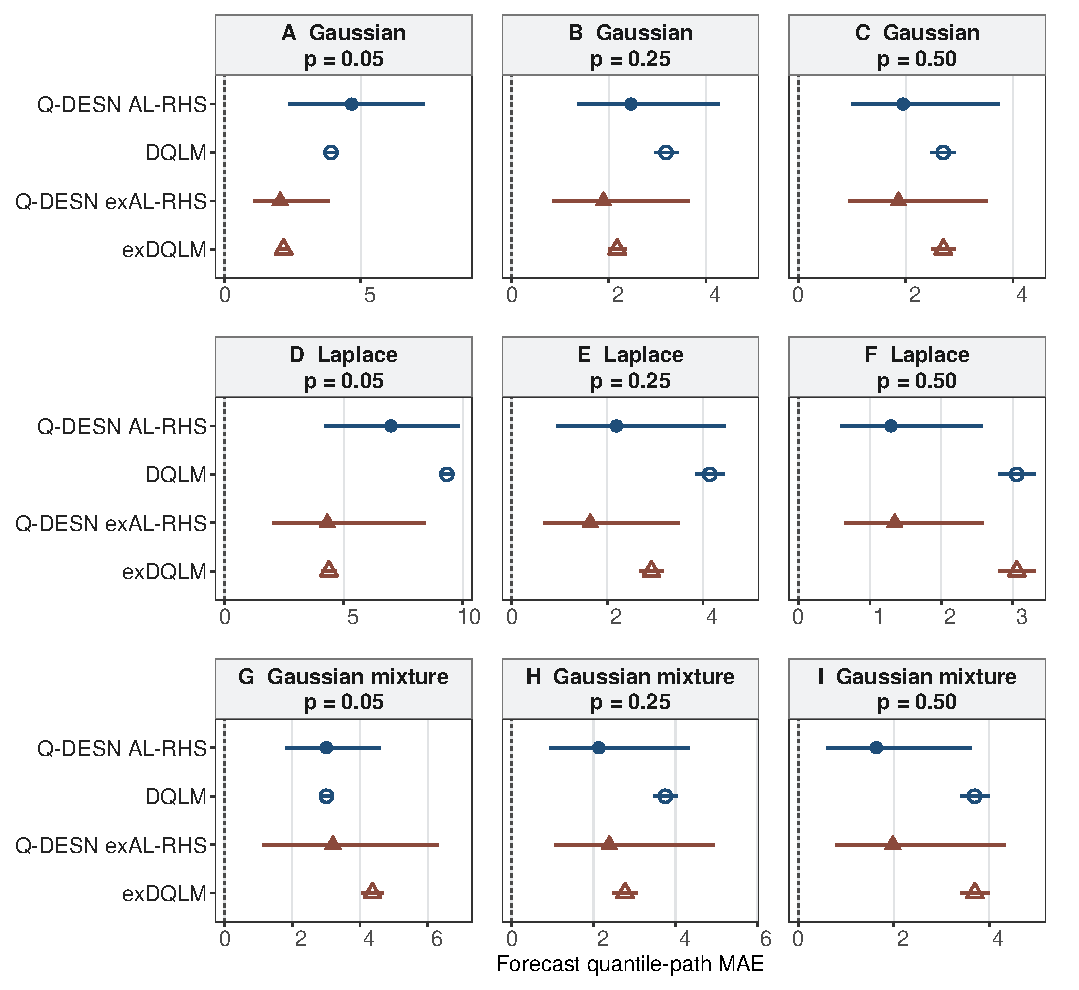
\includegraphics[width=0.98\textwidth]{figures/ch04-qdesn/independent_simulation/independent_train500_eval300_mcmc_forecast_mae_v1.pdf}
\caption{MCMC forecast quantile-path MAE over the first 300 evaluation targets (10 origins). Points and equal-tailed 95\% intervals summarize the draw-wise criterion averaged over scored pairs; lower is better. Navy circles identify \(\AL\) models and muted-brick triangles \(\exAL\) models; filled symbols denote Q--DESN and open symbols their dynamic linear comparators. Panels A--I identify the observation-error family and probability level. The dashed line marks exact recovery of the state-conditional quantile path. Panel scales match the 500-target sensitivity figures. The integrated material documents criterion-specific selection and model-specific forecast-draw dependence.}
\figalt{Nine panels compare four models using mean forecast quantile-path MAE and 95 percent intervals over 300 scored targets.}
\label{qdesn2026:fig:simulation-500obs-mcmc-forecast-mae-intervals}
\end{figure}



Figures~\ref{qdesn2026:fig:simulation-500obs-mcmc-fit-rmse-intervals} and
\ref{qdesn2026:fig:simulation-500obs-vb-fit-rmse-intervals} isolate fitting-sample
quantile-path recovery. They complement the MCMC forecast comparisons in the
main article by evaluating the estimated quantile path over the fitting sample.

\begin{figure}[!htbp]
\centering
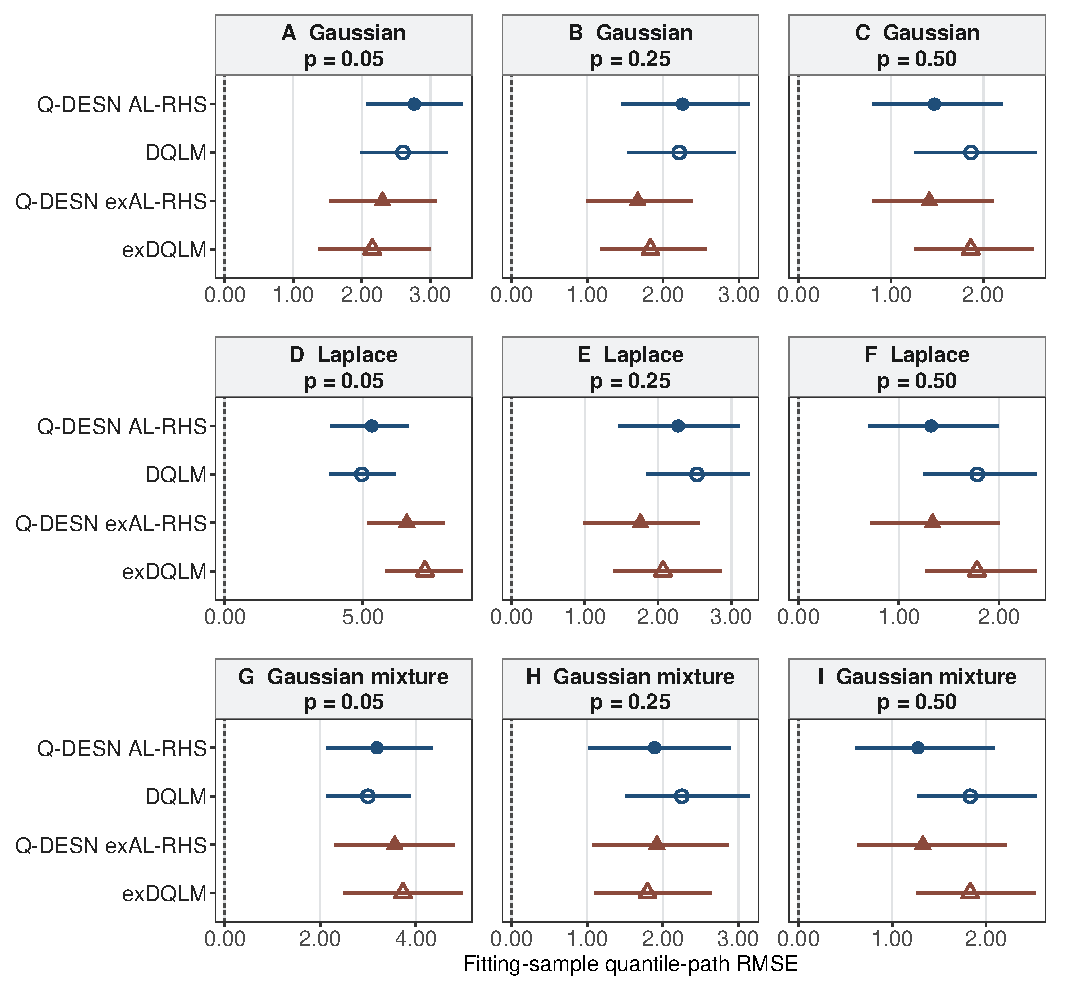
\includegraphics[width=0.98\textwidth]{figures/ch04-qdesn/independent_simulation/qdesn_pro_review_mcmc_fit_rmse.pdf}
\caption{MCMC fitting-sample recovery in the single-quantile study. Points and equal-tailed 95\% intervals summarize draw-wise quantile-path root mean squared error (RMSE); lower values are better. Navy circles identify \(\AL\) models and muted-brick triangles \(\exAL\) models; filled symbols denote Q--DESN and open symbols their dynamic linear comparators. Panels A--I identify the observation-error family and probability level, with separate horizontal scales. The dashed line marks exact recovery. The summaries condition on the simulated series and the criterion-specific specification.}
\figalt{Nine panels compare posterior fitting-sample quantile-path RMSE means
and 95 percent intervals for four models across three observation-error families and
three probability levels. Lower values are better.}
\label{qdesn2026:fig:simulation-500obs-mcmc-fit-rmse-intervals}
\end{figure}


\begin{figure}[!htbp]
\centering
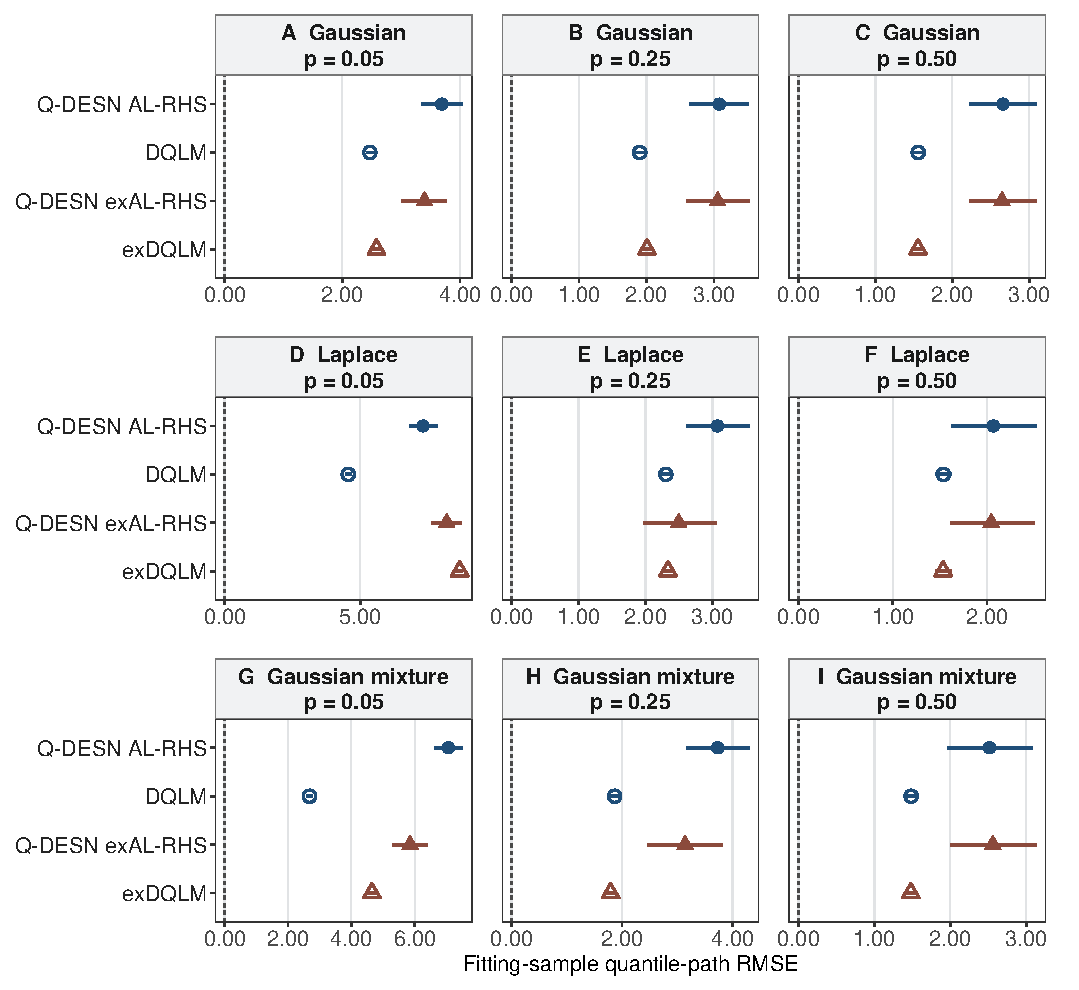
\includegraphics[width=0.98\textwidth]{figures/ch04-qdesn/independent_simulation/qdesn_pro_review_vb_fit_rmse.pdf}
\caption{Variational fitting-sample recovery in the single-quantile study. Points and approximate equal-tailed 95\% intervals summarize quantile-path RMSE under the variational fit; lower values are better. Model encodings follow Figure~\ref{qdesn2026:fig:simulation-500obs-mcmc-fit-rmse-intervals}. Panels A--I identify the observation-error family and probability level, with separate horizontal scales. The dashed line marks exact recovery. The summaries condition on the simulated series and the criterion-specific specification.}
\figalt{Nine panels compare approximate variational fitting-sample
quantile-path RMSE means and 95 percent intervals for four models across three
observation-error families and three probability levels. Lower values are better.}
\label{qdesn2026:fig:simulation-500obs-vb-fit-rmse-intervals}
\end{figure}



\subsubsection{Single-Quantile Evaluation Period Sensitivity}
\label{qdesn2026:subsec:supp-independent-evaluation-sensitivity}

The following analysis extends the scored target range from the first 300
to the first 500 observations after fitting, without changing the model
specification, fitted posterior, posterior-draw identities, or forecast
construction. Means and equal-tailed intervals are recomputed from draw-wise
aggregate scores over the relevant pairs; interval endpoints are not averaged.
The final origin is weighted by its 20 scored pairs rather than treated as a
complete 30-lead origin. The comparison is a sensitivity analysis of evaluation
scope, not an improvement to the fitted model or a separate validation sample.

\begin{figure}[!htbp]
\centering
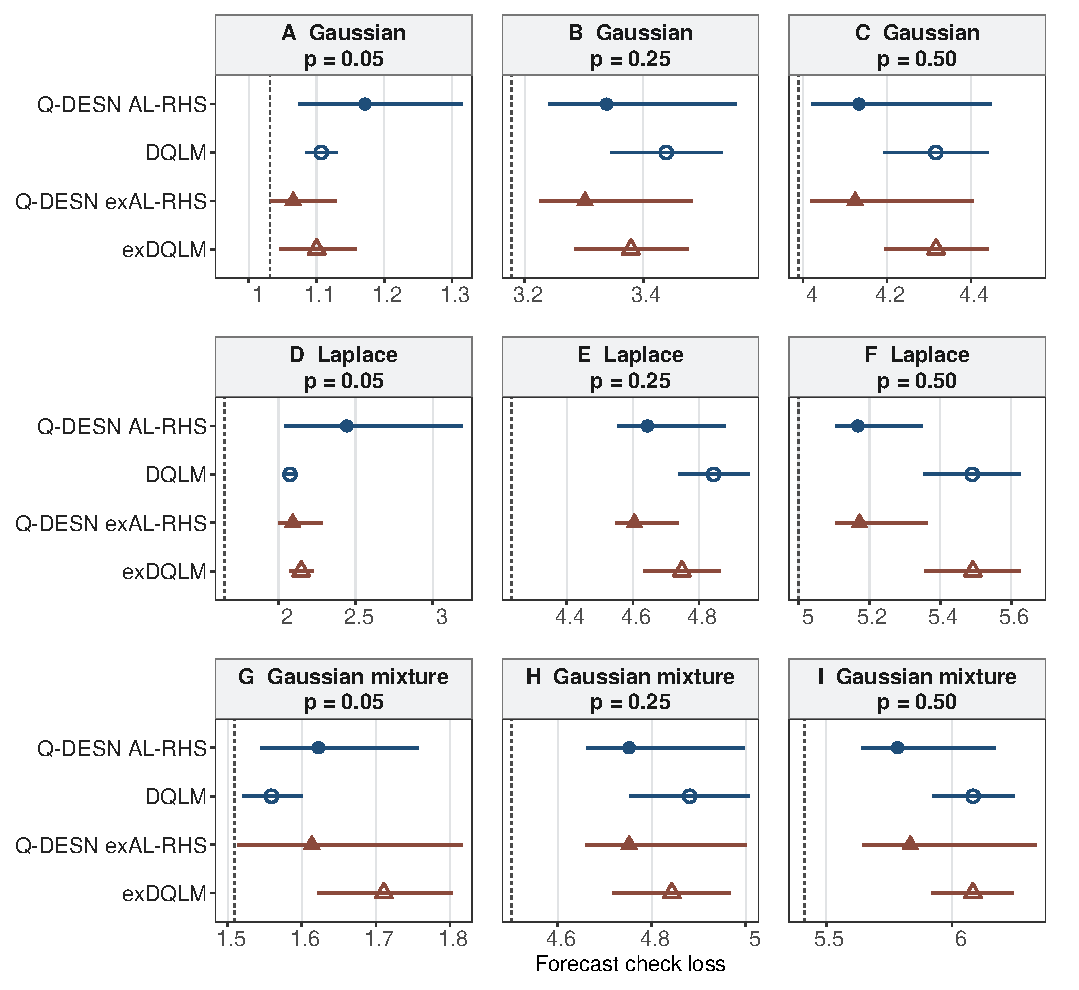
\includegraphics[width=0.98\textwidth]{figures/ch04-qdesn/independent_simulation/independent_train500_eval500_mcmc_forecast_check_v1.pdf}
\caption{MCMC forecast check loss over the first 500 evaluation targets (17 origins). Points and equal-tailed 95\% intervals summarize the draw-wise criterion averaged over scored pairs; lower is better. Navy circles identify \(\AL\) models and muted-brick triangles \(\exAL\) models; filled symbols denote Q--DESN and open symbols their dynamic linear comparators. Panels A--I identify the observation-error family and probability level. The dashed line marks population expected check loss at the true conditional quantile, not a finite-sample lower bound. The last origin contributes 20 leads; earlier origins contribute 30. The integrated material documents criterion-specific selection and model-specific forecast-draw dependence.}
\figalt{Nine panels compare four models using mean forecast check loss and 95 percent intervals over 500 scored targets.}
\label{qdesn2026:fig:independent-eval500-forecast_check}
\end{figure}

\begin{table}[!htbp]
\centering
\scriptsize
\setstretch{1}
\setlength{\tabcolsep}{4pt}
\begin{tabular}{@{}clcc@{}}
\toprule
Target & Model & Forecast MAE & Forecast check loss \\
\midrule
$p=0.05$ & DQLM & \shortstack{3.953\\{\scriptsize [3.808, 4.100]}} & \shortstack{1.107\\{\scriptsize [1.084, 1.131]}} \\
 & exDQLM & \shortstack{\textbf{2.401}\\{\scriptsize [2.243, 2.564]}} & \shortstack{1.100\\{\scriptsize [1.045, 1.158]}} \\
 & Q--DESN AL--RHS & \shortstack{5.421\\{\scriptsize [2.468, 8.741]}} & \shortstack{1.172\\{\scriptsize [1.074, 1.316]}} \\
 & Q--DESN exAL--RHS & \shortstack{2.408\\{\scriptsize [1.110, 4.914]}} & \shortstack{\textbf{1.066}\\{\scriptsize [1.032, 1.130]}} \\
\addlinespace[2pt]
$p=0.25$ & DQLM & \shortstack{3.143\\{\scriptsize [2.952, 3.334]}} & \shortstack{3.439\\{\scriptsize [3.344, 3.534]}} \\
 & exDQLM & \shortstack{2.316\\{\scriptsize [2.165, 2.470]}} & \shortstack{3.379\\{\scriptsize [3.283, 3.477]}} \\
 & Q--DESN AL--RHS & \shortstack{2.606\\{\scriptsize [1.376, 4.895]}} & \shortstack{3.338\\{\scriptsize [3.240, 3.557]}} \\
 & Q--DESN exAL--RHS & \shortstack{\textbf{2.163}\\{\scriptsize [0.8941, 4.437]}} & \shortstack{\textbf{3.302}\\{\scriptsize [3.225, 3.483]}} \\
\addlinespace[2pt]
$p=0.50$ & DQLM & \shortstack{2.710\\{\scriptsize [2.534, 2.891]}} & \shortstack{4.316\\{\scriptsize [4.191, 4.441]}} \\
 & exDQLM & \shortstack{2.715\\{\scriptsize [2.539, 2.894]}} & \shortstack{4.317\\{\scriptsize [4.193, 4.441]}} \\
 & Q--DESN AL--RHS & \shortstack{2.152\\{\scriptsize [1.021, 4.438]}} & \shortstack{4.133\\{\scriptsize [4.021, 4.450]}} \\
 & Q--DESN exAL--RHS & \shortstack{\textbf{2.068}\\{\scriptsize [0.9650, 4.198]}} & \shortstack{\textbf{4.124}\\{\scriptsize [4.019, 4.406]}} \\
\bottomrule
\end{tabular}
\caption{Sensitivity MCMC metric summaries for the Gaussian family. Forecast criteria use the first 500 scored targets; entries are posterior means with equal-tailed 95\% intervals. The models and posterior draws are the same as in the primary comparison. Lower is better; boldface marks the lowest unrounded mean within each target level and criterion. Intervals condition on the selected specification and data.}
\label{qdesn2026:tab:independent-eval500-mcmc-normal}
\end{table}

\begin{table}[!htbp]
\centering
\scriptsize
\setstretch{1}
\setlength{\tabcolsep}{4pt}
\begin{tabular}{@{}clcc@{}}
\toprule
Target & Model & Forecast MAE & Forecast check loss \\
\midrule
$p=0.05$ & DQLM & \shortstack{9.700\\{\scriptsize [9.449, 9.950]}} & \shortstack{\textbf{2.075}\\{\scriptsize [2.031, 2.120]}} \\
 & exDQLM & \shortstack{4.688\\{\scriptsize [4.436, 4.942]}} & \shortstack{2.148\\{\scriptsize [2.069, 2.226]}} \\
 & Q--DESN AL--RHS & \shortstack{7.158\\{\scriptsize [4.422, 9.992]}} & \shortstack{2.443\\{\scriptsize [2.038, 3.193]}} \\
 & Q--DESN exAL--RHS & \shortstack{\textbf{4.045}\\{\scriptsize [1.936, 8.639]}} & \shortstack{2.093\\{\scriptsize [1.998, 2.288]}} \\
\addlinespace[2pt]
$p=0.25$ & DQLM & \shortstack{4.096\\{\scriptsize [3.862, 4.334]}} & \shortstack{4.844\\{\scriptsize [4.737, 4.953]}} \\
 & exDQLM & \shortstack{3.007\\{\scriptsize [2.817, 3.205]}} & \shortstack{4.749\\{\scriptsize [4.633, 4.865]}} \\
 & Q--DESN AL--RHS & \shortstack{2.358\\{\scriptsize [1.030, 4.972]}} & \shortstack{4.644\\{\scriptsize [4.554, 4.880]}} \\
 & Q--DESN exAL--RHS & \shortstack{\textbf{1.785}\\{\scriptsize [0.7216, 3.985]}} & \shortstack{\textbf{4.605}\\{\scriptsize [4.546, 4.739]}} \\
\addlinespace[2pt]
$p=0.50$ & DQLM & \shortstack{3.121\\{\scriptsize [2.923, 3.323]}} & \shortstack{5.490\\{\scriptsize [5.353, 5.625]}} \\
 & exDQLM & \shortstack{3.125\\{\scriptsize [2.925, 3.332]}} & \shortstack{5.492\\{\scriptsize [5.355, 5.627]}} \\
 & Q--DESN AL--RHS & \shortstack{\textbf{1.425}\\{\scriptsize [0.6121, 3.052]}} & \shortstack{\textbf{5.167}\\{\scriptsize [5.105, 5.350]}} \\
 & Q--DESN exAL--RHS & \shortstack{1.489\\{\scriptsize [0.6836, 3.100]}} & \shortstack{5.172\\{\scriptsize [5.106, 5.364]}} \\
\bottomrule
\end{tabular}
\caption{Sensitivity MCMC metric summaries for the Laplace family. Forecast criteria use the first 500 scored targets; entries are posterior means with equal-tailed 95\% intervals. The models and posterior draws are the same as in the primary comparison. Lower is better; boldface marks the lowest unrounded mean within each target level and criterion. Intervals condition on the selected specification and data.}
\label{qdesn2026:tab:independent-eval500-mcmc-laplace}
\end{table}

\begin{table}[!htbp]
\centering
\scriptsize
\setstretch{1}
\setlength{\tabcolsep}{4pt}
\begin{tabular}{@{}clcc@{}}
\toprule
Target & Model & Forecast MAE & Forecast check loss \\
\midrule
$p=0.05$ & DQLM & \shortstack{\textbf{3.213}\\{\scriptsize [3.039, 3.388]}} & \shortstack{\textbf{1.559}\\{\scriptsize [1.519, 1.600]}} \\
 & exDQLM & \shortstack{4.694\\{\scriptsize [4.427, 4.956]}} & \shortstack{1.711\\{\scriptsize [1.622, 1.803]}} \\
 & Q--DESN AL--RHS & \shortstack{3.269\\{\scriptsize [1.891, 5.325]}} & \shortstack{1.623\\{\scriptsize [1.545, 1.758]}} \\
 & Q--DESN exAL--RHS & \shortstack{3.346\\{\scriptsize [1.133, 7.027]}} & \shortstack{1.613\\{\scriptsize [1.513, 1.817]}} \\
\addlinespace[2pt]
$p=0.25$ & DQLM & \shortstack{3.726\\{\scriptsize [3.497, 3.961]}} & \shortstack{4.881\\{\scriptsize [4.752, 5.008]}} \\
 & exDQLM & \shortstack{3.026\\{\scriptsize [2.775, 3.271]}} & \shortstack{4.843\\{\scriptsize [4.716, 4.968]}} \\
 & Q--DESN AL--RHS & \shortstack{\textbf{2.365}\\{\scriptsize [0.9736, 5.169]}} & \shortstack{\textbf{4.752}\\{\scriptsize [4.662, 4.998]}} \\
 & Q--DESN exAL--RHS & \shortstack{2.649\\{\scriptsize [1.104, 5.805]}} & \shortstack{4.752\\{\scriptsize [4.659, 5.001]}} \\
\addlinespace[2pt]
$p=0.50$ & DQLM & \shortstack{3.738\\{\scriptsize [3.503, 3.981]}} & \shortstack{6.084\\{\scriptsize [5.923, 6.250]}} \\
 & exDQLM & \shortstack{3.742\\{\scriptsize [3.507, 3.984]}} & \shortstack{6.083\\{\scriptsize [5.920, 6.246]}} \\
 & Q--DESN AL--RHS & \shortstack{\textbf{1.793}\\{\scriptsize [0.6319, 4.203]}} & \shortstack{\textbf{5.784}\\{\scriptsize [5.638, 6.172]}} \\
 & Q--DESN exAL--RHS & \shortstack{2.161\\{\scriptsize [0.8021, 4.992]}} & \shortstack{5.834\\{\scriptsize [5.645, 6.335]}} \\
\bottomrule
\end{tabular}
\caption{Sensitivity MCMC metric summaries for the Gaussian mixture family. Forecast criteria use the first 500 scored targets; entries are posterior means with equal-tailed 95\% intervals. The models and posterior draws are the same as in the primary comparison. Lower is better; boldface marks the lowest unrounded mean within each target level and criterion. Intervals condition on the selected specification and data.}
\label{qdesn2026:tab:independent-eval500-mcmc-gausmix}
\end{table}




\subsubsection{Single-Quantile Empirical Frequencies}
\label{qdesn2026:subsec:supp-independent-calibration}

We also examine whether the nominal quantile levels agree with empirical
response frequencies, complementing the check-loss comparisons
\citep{qdesn-GneitingResin2023Calibration}. For each model and case, we retain the
specification used for check loss and summarize its pooled posterior
quantile-location draws at each forecast target by their median:
\begingroup\scriptsize\begin{align}
\text{Reported quantile:}\quad
&\widehat q_{p,\ell}=\operatorname{median}_{b}\{q_{p,\ell}^{(b)}\},\\
\text{Empirical frequency:}\quad
&\widehat c_p=\frac{1}{N_{\mathrm{eval}}}
\sum_{\ell=1}^{N_{\mathrm{eval}}}
\ind\{y_\ell\leq\widehat q_{p,\ell}\}.
\end{align}\endgroup
The nominal reference is \(p\). Both evaluation periods use the same
target-specific forecasts; the 500-target analysis simply includes more
observed forecast pairs. These frequencies describe agreement over the
evaluation record rather than posterior uncertainty in a score or a test
of conditional calibration.

At the median, Q--DESN frequencies are close to 50\% under Laplace errors
but around 41\% under Gaussian-mixture errors in both evaluation periods;
the dynamic comparators remain near 50\% in the latter case. At the 5\%
level under Gaussian errors, the exAL Q--DESN frequency increases from
3.3\% over 300 targets to 4.8\% over 500 targets. Its frequencies remain
above 5\% for the Laplace and Gaussian-mixture cases.

\begin{figure}[!htbp]
\centering
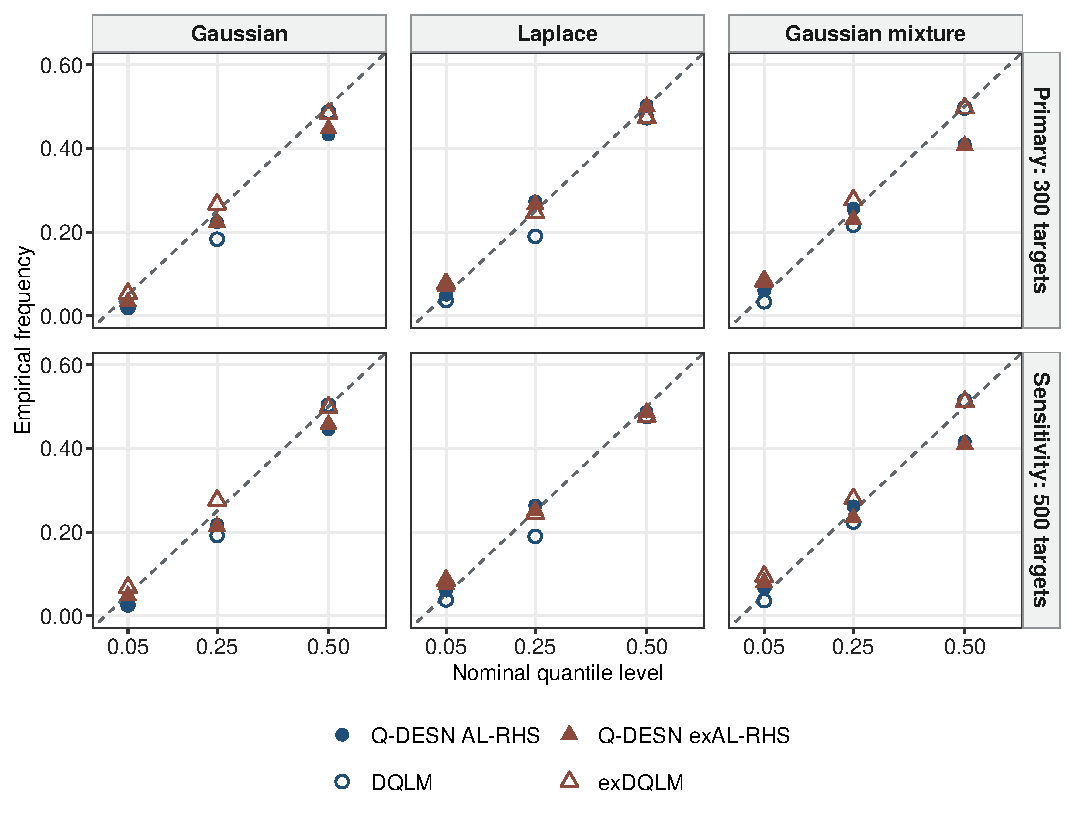
\includegraphics[width=0.98\textwidth]{figures/ch04-qdesn/independent_simulation/independent_forecast_calibration_v1.pdf}
\caption{Empirical quantile frequencies over the 300-target primary period and its 500-target extension. Each model uses the same specification as in the check-loss comparison. At each target, the quantile forecast is the posterior median, pooling the three chains. Points give the fractions of responses at or below these forecasts; the dashed diagonal marks the nominal probability. Colours and symbols follow the forecast-score figures. Each probability level uses its corresponding quantile-centred response series. No sampling confidence bands are shown.}
\figalt{Six panels compare empirical response frequencies below posterior-median quantile forecasts with the nominal levels 0.05, 0.25 and 0.50, for four models, three error families and two evaluation periods.}
\label{qdesn2026:fig:supp-independent-quantile-calibration}
\end{figure}

\begin{table}[!htbp]
\centering
\footnotesize
\setstretch{1}
\setlength{\tabcolsep}{3.5pt}
\begin{tabular}{@{}llcrrrr@{}}
\toprule
Targets & Error family & $p$ & DQLM & exDQLM & \shortstack{Q--DESN\\AL} & \shortstack{Q--DESN\\exAL} \\
\midrule
300 & Gaussian & 0.05 & 2.0 (6) & 5.3 (16) & 2.0 (6) & 3.3 (10) \\
 &  & 0.25 & 18.3 (55) & 26.7 (80) & 22.3 (67) & 22.3 (67) \\
 &  & 0.50 & 48.7 (146) & 48.3 (145) & 43.3 (130) & 44.7 (134) \\
\addlinespace[3pt]
 & Laplace & 0.05 & 3.7 (11) & 7.7 (23) & 5.0 (15) & 7.0 (21) \\
 &  & 0.25 & 19.0 (57) & 24.7 (74) & 27.3 (82) & 26.7 (80) \\
 &  & 0.50 & 47.3 (142) & 47.3 (142) & 50.3 (151) & 50.0 (150) \\
\addlinespace[3pt]
 & Gaussian mixture & 0.05 & 3.3 (10) & 8.3 (25) & 6.0 (18) & 8.0 (24) \\
 &  & 0.25 & 21.7 (65) & 27.7 (83) & 25.7 (77) & 23.0 (69) \\
 &  & 0.50 & 49.7 (149) & 49.7 (149) & 41.0 (123) & 40.7 (122) \\
\addlinespace[3pt]
500 & Gaussian & 0.05 & 2.6 (13) & 6.8 (34) & 2.4 (12) & 4.8 (24) \\
 &  & 0.25 & 19.2 (96) & 27.6 (138) & 21.8 (109) & 21.4 (107) \\
 &  & 0.50 & 50.4 (252) & 49.8 (249) & 44.6 (223) & 45.8 (229) \\
\addlinespace[3pt]
 & Laplace & 0.05 & 3.8 (19) & 8.4 (42) & 6.0 (30) & 7.4 (37) \\
 &  & 0.25 & 19.0 (95) & 24.4 (122) & 26.4 (132) & 25.2 (126) \\
 &  & 0.50 & 47.6 (238) & 47.6 (238) & 48.8 (244) & 48.6 (243) \\
\addlinespace[3pt]
 & Gaussian mixture & 0.05 & 3.6 (18) & 9.4 (47) & 6.6 (33) & 8.0 (40) \\
 &  & 0.25 & 22.4 (112) & 28.0 (140) & 26.2 (131) & 23.4 (117) \\
 &  & 0.50 & 51.4 (257) & 51.2 (256) & 41.6 (208) & 41.0 (205) \\
\bottomrule
\end{tabular}
\caption{Empirical quantile frequencies in percent, followed by the number of responses at or below the forecast in parentheses. The target count is the denominator. Forecasts are posterior-median quantile locations from the existing check-loss specifications; no model is selected using these frequencies.}
\label{qdesn2026:tab:supp-independent-quantile-calibration}
\end{table}



\subsubsection{Single-Quantile Computation and Diagnostics}
\label{qdesn2026:subsec:supp-independent-exal-mcmc-details}

The independent Q--DESN exAL--RHS MCMC analysis uses the mixture representation
for \(v\) described earlier in this appendix and an analysis-specific
scale-collapsed transition. Conditional on the remaining unknowns, the scale is
integrated from the conditional density used to update the asymmetry parameter
on a logit transformation of its bounded support, and the scale is then drawn
from its full conditional distribution. This transition is used for the
independent simulation analysis; Algorithm~\ref{qdesn2026:alg:qdesn_mcmc} gives the generic joint or
conditionally split update. The resulting draws determine the fitted and
forecast quantile paths used in the reported criteria.

The exDQLM baseline was refreshed under version 1.1.1 of the CRAN package
\pkg{exdqlm} \citep{env-deleon2026exdqlm}. The inherited Q--DESN execution
records identify version 1.0.0; those fits were not part of the scoped
exDQLM refresh. For unrestricted exAL fits, the exDQLM MCMC sampler updates
the asymmetry parameter from its conditional
distribution with the scale analytically integrated out, then draws the scale
from its full conditional distribution. Its variational calculation uses the
structured factorization \(q(\gamma)q(\sigma\mid\gamma)\). These model-specific
computations produce the
quantile-path draws evaluated by the common criteria above.
For retained pairs \((\sigma_b,\gamma_b)\),
\(b=1,\ldots,B_{\mathrm{post}}\), let
\begingroup\scriptsize\[
m_{\varepsilon,b}=\sigma_b\{A_p(\gamma_b)+D_p(\gamma_b)\sqrt{2/\pi}\},\qquad
V_{\varepsilon,b}=\sigma_b^2\{B_p(\gamma_b)+A_p(\gamma_b)^2
  +D_p(\gamma_b)^2(1-2/\pi)\}.
\]\endgroup
The rolling-origin filter uses
\(\bar m_\varepsilon=B_{\mathrm{post}}^{-1}\sum_b m_{\varepsilon,b}\) and
\(\bar V_\varepsilon=B_{\mathrm{post}}^{-1}
\sum_b(V_{\varepsilon,b}+m_{\varepsilon,b}^2)-\bar m_\varepsilon^2\).
The parameter posterior from the initial fit is retained, while observations
available at successive origins update the state filter before forecasts are
propagated over the requested horizons.

The MCMC metric distributions generally pool 12,000 retained evaluations from
three independently initialized chains. The Q--DESN AL--RHS Gaussian
\(p=0.05\) forecast MAE and check-loss summaries use 3,000 retained evaluations
from three chains. Diagnostics assess between-chain agreement for each
draw-wise criterion.


\subsubsection{Multiquantile MCMC Evaluation Details}

Eight mechanisms cover Gaussian, Laplace, Gaussian-mixture, asymmetric-tail,
persistent-heavy-tail, Student-\(t\), regime-shift, and nonlinear dynamics.
The seven levels are \(0.05\), \(0.10\), \(0.25\), \(0.50\),
\(0.75\), \(0.90\), and \(0.95\). Each regression uses 500 fitting
observations and 990 forecast pairs, from 33 origins and 30 horizons per
origin. The regressions use the initialization sequence in
Figure~\ref{qdesn2026:fig:supp-quantile-sequential-initialization}. One scenario-specific
DESN/RHS specification is selected using separately simulated series and held common
across Q--DESN and MQ--DESN under the AL and exAL likelihoods.
The readout includes every reservoir layer
and an intercept, while response lags enter only through reservoir inputs.
The evaluation realization is used for the final fit and evaluation.
Table~\ref{qdesn2026:tab:joint-qdesn-pure-desn-v2-protocol} records the variational
components, five-chain MCMC allocation, and scoring draws. All chains within
a model and mechanism use the same data, likelihood, and prior
hyperparameters; only their starting values differ. Every \(\exAL\)
chain uses the exact scale-collapsed MCMC transition described above.
Intercept prior centers and scales are calibrated once from the Gaussian
reference fit and held common across the four regressions and all chains;
MQ--DESN intercepts are ordered. The first quantile slope anchors the RHS hierarchy,
with no additional latent baseline.
Writing \(q_G\) for the Gaussian RHS variational reference, the fixed
calibration quantities are
\begin{equation}
\begin{aligned}
\text{Reference residual scale:}\quad
&s_G=\sqrt{\E_{q_G}(\sigma_G^2)},\\
\text{Intercept prior center:}\quad
&b_{0k}=\E_{q_G}(\beta_{0G})+s_G\Phi^{-1}(p_k),\\
\text{Intercept prior variance:}\quad
&V_{0k}=(2s_G)^2.
\end{aligned}
\label{qdesn2026:eq:supp-joint-intercept-calibration}
\end{equation}
These data-calibrated priors are not the Gaussian initializer's separate
intercept variance \(10^6\), nor are they chain-specific starting values.
The \(\exAL\) variational initializers use the \(v\) augmentation and the
structured factor \(q(\gamma_k)q(\sigma_k\mid\gamma_k)\) in
Section~\ref{qdesn2026:subsec:supp_structured_exal_vb}. Scale integration is analytic;
quadrature over the bounded shape support supplies its normalization and
mixed moments.

\begin{table}[!htbp]
\centering
\scriptsize
\setlength{\tabcolsep}{3pt}
\renewcommand{\arraystretch}{1.08}
\begin{tabular}{@{}>{\raggedright\arraybackslash}p{0.23\textwidth}>{\raggedright\arraybackslash}p{0.68\textwidth}@{}}
\toprule
Item & Specification \\
\midrule
Reservoir specification & One reservoir specification per setting, selected using separately simulated series and shared across all four regressions. The regression uses an intercept and the states from all reservoir layers. \\
Quantile levels & 0.05, 0.10, 0.25, 0.50, 0.75, 0.90, and 0.95; trapezoidal weights sum to 0.90. \\
Forecast design & 33 origins and 30 horizons, giving 990 origin--horizon pairs per setting. Observed histories update states between origins; future response lags are generated recursively within each origin. \\
Posterior simulation & Five chains per model and mechanism. Scores use 3,750 pooled AL draws and 3,750 exAL draws, except 7,500 exAL draws for Laplace. All exAL chains use the exact scale-collapsed asymmetry transition. \\
Initialization & Gaussian, AL, exAL, and MQ--DESN fits supply starting values in the stated sequence. Prior hyperparameters define each target and are common across its five chains. \\
Uncertainty & Primary intervals condition on each model's averaged future predictor matrix; trajectory-inclusive intervals are reported separately. VB intervals additionally condition on fixed intercept estimates. \\
Computation & Score calculations are finite for all 64 method--model comparisons; the 32 MCMC comparisons meet the stated score-stability criteria. These checks do not establish complete scalar-parameter mixing. \\
\bottomrule
\end{tabular}
\caption{Design and computation for the multiquantile study.}
\label{qdesn2026:tab:joint-qdesn-pure-desn-v2-protocol}
\end{table}

\begingroup
\footnotesize
\setlength{\tabcolsep}{3pt}
\renewcommand{\arraystretch}{1.08}
\begin{longtable}{@{}>{\raggedright\arraybackslash}p{0.18\textwidth}>{\raggedright\arraybackslash}p{0.14\textwidth}*{4}{>{\raggedleft\arraybackslash}p{0.09\textwidth}}>{\raggedleft\arraybackslash}p{0.125\textwidth}@{}}
\caption{Oracle finite-grid \(\aCRPS\) in the multiquantile study. Means, medians, and equal-tailed 95\% limits summarize posterior coefficient and intercept uncertainty conditional on each model's averaged future predictor matrix. The mean-grid score evaluates the projected posterior-mean quantile grid and differs from the posterior mean of the score. Boldface identifies numerical minima; all winner and runner-up marginal intervals overlap. Q--DESN fits levels independently; MQ--DESN estimates their coefficients jointly.}\label{qdesn2026:tab:joint-qdesn-pure-desn-v2-score}\\
\toprule
Simulation setting & Model & Mean & Median & 2.5\% & 97.5\% & \shortstack{Mean-grid\\score} \\
\midrule
\endfirsthead
\caption[]{Continued.}\\
\toprule
Simulation setting & Model & Mean & Median & 2.5\% & 97.5\% & \shortstack{Mean-grid\\score} \\
\midrule
\endhead
\midrule
\multicolumn{7}{r}{\footnotesize Continued on next page}\\
\endfoot
\bottomrule
\endlastfoot
Asymmetric-Laplace tail & MQ--DESN (AL) & 0.3805 & 0.3790 & 0.3705 & 0.3985 & 0.3768 \\
 & Q--DESN (AL) & 0.4160 & 0.4153 & 0.3910 & 0.4435 & 0.4136 \\
 & MQ--DESN (exAL) & \textbf{0.3737} & 0.3724 & 0.3676 & 0.3858 & 0.3705 \\
 & Q--DESN (exAL) & 0.4323 & 0.4319 & 0.3998 & 0.4683 & 0.4268 \\
\addlinespace[2pt]
Gaussian-mixture innovations & MQ--DESN (AL) & 0.4609 & 0.4595 & 0.4463 & 0.4826 & 0.4563 \\
 & Q--DESN (AL) & \textbf{0.4518} & 0.4505 & 0.4385 & 0.4728 & 0.4449 \\
 & MQ--DESN (exAL) & 0.4687 & 0.4679 & 0.4518 & 0.4906 & 0.4657 \\
 & Q--DESN (exAL) & 0.4551 & 0.4538 & 0.4383 & 0.4798 & 0.4471 \\
\addlinespace[2pt]
Laplace innovations & MQ--DESN (AL) & 0.3627 & 0.3626 & 0.3606 & 0.3651 & 0.3617 \\
 & Q--DESN (AL) & \textbf{0.3613} & 0.3612 & 0.3589 & 0.3641 & 0.3597 \\
 & MQ--DESN (exAL) & 0.3626 & 0.3624 & 0.3600 & 0.3653 & 0.3611 \\
 & Q--DESN (exAL) & 0.3627 & 0.3626 & 0.3597 & 0.3660 & 0.3609 \\
\addlinespace[2pt]
Nonlinear reservoir dynamics & MQ--DESN (AL) & 0.5001 & 0.4984 & 0.4843 & 0.5250 & 0.4933 \\
 & Q--DESN (AL) & \textbf{0.4881} & 0.4871 & 0.4787 & 0.5031 & 0.4807 \\
 & MQ--DESN (exAL) & 0.5003 & 0.4995 & 0.4858 & 0.5201 & 0.4970 \\
 & Q--DESN (exAL) & 0.4969 & 0.4959 & 0.4823 & 0.5170 & 0.4888 \\
\addlinespace[2pt]
Gaussian innovations & MQ--DESN (AL) & \textbf{0.3495} & 0.3481 & 0.3431 & 0.3633 & 0.3471 \\
 & Q--DESN (AL) & 0.3638 & 0.3630 & 0.3481 & 0.3846 & 0.3573 \\
 & MQ--DESN (exAL) & 0.3563 & 0.3547 & 0.3442 & 0.3768 & 0.3536 \\
 & Q--DESN (exAL) & 0.3553 & 0.3541 & 0.3429 & 0.3753 & 0.3452 \\
\addlinespace[2pt]
Persistent heavy tails & MQ--DESN (AL) & 1.1239 & 1.1113 & 0.9398 & 1.3707 & 1.1089 \\
 & Q--DESN (AL) & \textbf{1.0544} & 1.0489 & 0.8777 & 1.2635 & 1.0474 \\
 & MQ--DESN (exAL) & 1.0789 & 1.0736 & 0.9017 & 1.2856 & 1.0693 \\
 & Q--DESN (exAL) & 1.1022 & 1.0979 & 0.9268 & 1.3064 & 1.1007 \\
\addlinespace[2pt]
Regime shift & MQ--DESN (AL) & 1.1555 & 1.1543 & 0.8992 & 1.4205 & 1.1488 \\
 & Q--DESN (AL) & 1.0531 & 1.0508 & 0.9106 & 1.2048 & 1.0532 \\
 & MQ--DESN (exAL) & 1.0394 & 1.0412 & 0.8108 & 1.2538 & 1.0327 \\
 & Q--DESN (exAL) & \textbf{1.0307} & 1.0293 & 0.8774 & 1.1895 & 1.0251 \\
\addlinespace[2pt]
Student-\(t\) location--scale & MQ--DESN (AL) & 0.3983 & 0.3982 & 0.3964 & 0.4005 & 0.3972 \\
 & Q--DESN (AL) & \textbf{0.3973} & 0.3972 & 0.3954 & 0.3995 & 0.3962 \\
 & MQ--DESN (exAL) & 0.4014 & 0.4013 & 0.3981 & 0.4049 & 0.4003 \\
 & Q--DESN (exAL) & 0.4000 & 0.3999 & 0.3970 & 0.4034 & 0.3986 \\
\end{longtable}
\endgroup


\begingroup
\footnotesize
\setlength{\tabcolsep}{3pt}
\renewcommand{\arraystretch}{1.08}
\begin{longtable}{@{}>{\raggedright\arraybackslash}p{0.23\textwidth}>{\raggedright\arraybackslash}p{0.19\textwidth}*{2}{>{\raggedleft\arraybackslash}p{0.20\textwidth}}@{}}
\caption{Finite-grid \(\aCRPS\) against realized observations. Posterior mean scores condition on each model's averaged future predictors; the mean-grid score evaluates its projected posterior-mean quantile grid. These scores are secondary to oracle \(\aCRPS\). Q--DESN fits levels independently; MQ--DESN estimates their coefficients jointly.}\label{qdesn2026:tab:joint-qdesn-pure-desn-v2-secondary}\\
\toprule
Simulation setting & Model & \shortstack{Posterior mean\\realized score} & \shortstack{Mean-grid\\realized score} \\
\midrule
\endfirsthead
\caption[]{Continued.}\\
\toprule
Simulation setting & Model & \shortstack{Posterior mean\\realized score} & \shortstack{Mean-grid\\realized score} \\
\midrule
\endhead
\midrule
\multicolumn{4}{r}{\footnotesize Continued on next page}\\
\endfoot
\bottomrule
\endlastfoot
Asymmetric-Laplace tail & MQ--DESN (AL) & 0.3825 & 0.3789 \\
 & Q--DESN (AL) & 0.4175 & 0.4152 \\
 & MQ--DESN (exAL) & 0.3755 & 0.3723 \\
 & Q--DESN (exAL) & 0.4315 & 0.4259 \\
\addlinespace[2pt]
Gaussian-mixture innovations & MQ--DESN (AL) & 0.4701 & 0.4656 \\
 & Q--DESN (AL) & 0.4613 & 0.4543 \\
 & MQ--DESN (exAL) & 0.4772 & 0.4742 \\
 & Q--DESN (exAL) & 0.4651 & 0.4573 \\
\addlinespace[2pt]
Laplace innovations & MQ--DESN (AL) & 0.3467 & 0.3455 \\
 & Q--DESN (AL) & 0.3408 & 0.3391 \\
 & MQ--DESN (exAL) & 0.3459 & 0.3443 \\
 & Q--DESN (exAL) & 0.3407 & 0.3389 \\
\addlinespace[2pt]
Nonlinear reservoir dynamics & MQ--DESN (AL) & 0.5238 & 0.5172 \\
 & Q--DESN (AL) & 0.5140 & 0.5066 \\
 & MQ--DESN (exAL) & 0.5237 & 0.5204 \\
 & Q--DESN (exAL) & 0.5225 & 0.5144 \\
\addlinespace[2pt]
Gaussian innovations & MQ--DESN (AL) & 0.3578 & 0.3555 \\
 & Q--DESN (AL) & 0.3725 & 0.3661 \\
 & MQ--DESN (exAL) & 0.3665 & 0.3636 \\
 & Q--DESN (exAL) & 0.3651 & 0.3550 \\
\addlinespace[2pt]
Persistent heavy tails & MQ--DESN (AL) & 1.1220 & 1.1076 \\
 & Q--DESN (AL) & 1.0512 & 1.0446 \\
 & MQ--DESN (exAL) & 1.0751 & 1.0662 \\
 & Q--DESN (exAL) & 1.0976 & 1.0966 \\
\addlinespace[2pt]
Regime shift & MQ--DESN (AL) & 1.1528 & 1.1459 \\
 & Q--DESN (AL) & 1.0500 & 1.0499 \\
 & MQ--DESN (exAL) & 1.0355 & 1.0287 \\
 & Q--DESN (exAL) & 1.0284 & 1.0227 \\
\addlinespace[2pt]
Student-\(t\) location--scale & MQ--DESN (AL) & 0.4233 & 0.4224 \\
 & Q--DESN (AL) & 0.4228 & 0.4217 \\
 & MQ--DESN (exAL) & 0.4270 & 0.4260 \\
 & Q--DESN (exAL) & 0.4263 & 0.4249 \\
\end{longtable}
\endgroup


At each forecast origin, observed response lags reconstruct the reservoir
state. Future responses are generated by inverse sampling from the projected
quantile grid, with linear interpolation between fitted levels and the outermost
fitted quantiles used beyond the fitted probability range. The future feature
vectors are averaged over these
trajectories for each model. Coefficient and intercept draws evaluated at
the averaged features give the primary score distribution. This is a
conditional forecast-location summary; it is not generally the quantile
function of the complete posterior predictive distribution.

Table~\ref{qdesn2026:tab:joint-qdesn-pure-desn-v2-recursive-policy} compares this
summary with evaluating each coefficient draw along its own recursive path.
The conditional intervals are narrower in 28 of 32 comparisons, with median
width ratio 0.7364, reflecting the uncertainty retained by each construction.
VB intervals additionally condition on fixed variational intercept estimates,
while retaining the Gaussian slope-factor covariance.
\begingroup
\setlength{\abovecaptionskip}{0pt}
\begingroup
\footnotesize
\setlength{\tabcolsep}{3pt}
\renewcommand{\arraystretch}{1.08}
\begin{longtable}{@{}>{\raggedright\arraybackslash}p{0.18\textwidth}>{\raggedright\arraybackslash}p{0.14\textwidth}*{2}{>{\raggedleft\arraybackslash}p{0.28\textwidth}}@{}}
\caption{Oracle finite-grid \(\aCRPS\) under two treatments of future predictors. Entries are posterior means and equal-tailed 95\% intervals. Averaged-predictor scores condition on each model's mean future predictor matrix; trajectory-specific scores use each draw's recursively generated predictors. The intervals summarize different propagated uncertainties, not future-response interval coverage. Q--DESN fits levels independently; MQ--DESN estimates their coefficients jointly.}\label{qdesn2026:tab:joint-qdesn-pure-desn-v2-recursive-policy}\\
\toprule
Simulation setting & Model & Averaged design & Recursive trajectories \\
\midrule
\endfirsthead
\caption[]{Continued.}\\
\toprule
Simulation setting & Model & Averaged design & Recursive trajectories \\
\midrule
\endhead
\midrule
\multicolumn{4}{r}{\footnotesize Continued on next page}\\
\endfoot
\bottomrule
\endlastfoot
Asymmetric-Laplace tail & MQ--DESN (AL) & 0.3805 [0.3705, 0.3985] & 0.4057 [0.3928, 0.4287] \\
 & Q--DESN (AL) & 0.4160 [0.3910, 0.4435] & 0.4470 [0.4156, 0.4908] \\
 & MQ--DESN (exAL) & 0.3737 [0.3676, 0.3858] & 0.4017 [0.3892, 0.4291] \\
 & Q--DESN (exAL) & 0.4323 [0.3998, 0.4683] & 0.4557 [0.4098, 0.5151] \\
\addlinespace[2pt]
Gaussian-mixture innovations & MQ--DESN (AL) & 0.4609 [0.4463, 0.4826] & 0.4988 [0.4766, 0.5286] \\
 & Q--DESN (AL) & 0.4518 [0.4385, 0.4728] & 0.4745 [0.4569, 0.4998] \\
 & MQ--DESN (exAL) & 0.4687 [0.4518, 0.4906] & 0.4907 [0.4682, 0.5196] \\
 & Q--DESN (exAL) & 0.4551 [0.4383, 0.4798] & 0.4695 [0.4488, 0.4991] \\
\addlinespace[2pt]
Laplace innovations & MQ--DESN (AL) & 0.3627 [0.3606, 0.3651] & 0.3820 [0.3760, 0.3891] \\
 & Q--DESN (AL) & 0.3613 [0.3589, 0.3641] & 0.3752 [0.3698, 0.3814] \\
 & MQ--DESN (exAL) & 0.3626 [0.3600, 0.3653] & 0.3783 [0.3721, 0.3840] \\
 & Q--DESN (exAL) & 0.3627 [0.3597, 0.3660] & 0.3737 [0.3686, 0.3794] \\
\addlinespace[2pt]
Nonlinear reservoir dynamics & MQ--DESN (AL) & 0.5001 [0.4843, 0.5250] & 0.5197 [0.5000, 0.5520] \\
 & Q--DESN (AL) & 0.4881 [0.4787, 0.5031] & 0.5030 [0.4908, 0.5239] \\
 & MQ--DESN (exAL) & 0.5003 [0.4858, 0.5201] & 0.5156 [0.4959, 0.5467] \\
 & Q--DESN (exAL) & 0.4969 [0.4823, 0.5170] & 0.5081 [0.4905, 0.5349] \\
\addlinespace[2pt]
Gaussian innovations & MQ--DESN (AL) & 0.3495 [0.3431, 0.3633] & 0.3744 [0.3646, 0.3947] \\
 & Q--DESN (AL) & 0.3638 [0.3481, 0.3846] & 0.3874 [0.3702, 0.4180] \\
 & MQ--DESN (exAL) & 0.3563 [0.3442, 0.3768] & 0.3780 [0.3624, 0.4111] \\
 & Q--DESN (exAL) & 0.3553 [0.3429, 0.3753] & 0.3778 [0.3631, 0.4072] \\
\addlinespace[2pt]
Persistent heavy tails & MQ--DESN (AL) & 1.1239 [0.9398, 1.3707] & 1.1706 [1.0077, 1.3903] \\
 & Q--DESN (AL) & 1.0544 [0.8777, 1.2635] & 1.0886 [0.9294, 1.2726] \\
 & MQ--DESN (exAL) & 1.0789 [0.9017, 1.2856] & 1.1048 [0.9714, 1.2624] \\
 & Q--DESN (exAL) & 1.1022 [0.9268, 1.3064] & 1.1223 [0.9652, 1.2999] \\
\addlinespace[2pt]
Regime shift & MQ--DESN (AL) & 1.1555 [0.8992, 1.4205] & 1.1839 [0.8799, 1.5224] \\
 & Q--DESN (AL) & 1.0531 [0.9106, 1.2048] & 1.0713 [0.8987, 1.2699] \\
 & MQ--DESN (exAL) & 1.0394 [0.8108, 1.2538] & 1.0665 [0.7749, 1.3529] \\
 & Q--DESN (exAL) & 1.0307 [0.8774, 1.1895] & 1.0447 [0.8649, 1.2430] \\
\addlinespace[2pt]
Student-\(t\) location--scale & MQ--DESN (AL) & 0.3983 [0.3964, 0.4005] & 0.4431 [0.4343, 0.4527] \\
 & Q--DESN (AL) & 0.3973 [0.3954, 0.3995] & 0.4398 [0.4311, 0.4498] \\
 & MQ--DESN (exAL) & 0.4014 [0.3981, 0.4049] & 0.4400 [0.4320, 0.4489] \\
 & Q--DESN (exAL) & 0.4000 [0.3970, 0.4034] & 0.4393 [0.4309, 0.4490] \\
\end{longtable}
\endgroup

\endgroup
\begingroup
\footnotesize
\setlength{\tabcolsep}{3pt}
\renewcommand{\arraystretch}{1.08}
\begin{longtable}{@{}>{\raggedright\arraybackslash}p{0.18\textwidth}>{\raggedright\arraybackslash}p{0.14\textwidth}*{4}{>{\raggedleft\arraybackslash}p{0.09\textwidth}}>{\raggedleft\arraybackslash}p{0.125\textwidth}@{}}
\caption{Variational oracle finite-grid \(\aCRPS\). Means, medians, and approximate equal-tailed 95\% limits condition on fixed intercept estimates and each model's averaged future predictor matrix; intercept uncertainty is not included. The mean-grid score evaluates the projected variational-mean quantile grid. Q--DESN fits levels independently; MQ--DESN estimates their coefficients jointly.}\label{qdesn2026:tab:joint-qdesn-pure-desn-v2-vb-score}\\
\toprule
Simulation setting & Model & Mean & Median & 2.5\% & 97.5\% & \shortstack{Mean-grid\\score} \\
\midrule
\endfirsthead
\caption[]{Continued.}\\
\toprule
Simulation setting & Model & Mean & Median & 2.5\% & 97.5\% & \shortstack{Mean-grid\\score} \\
\midrule
\endhead
\midrule
\multicolumn{7}{r}{\footnotesize Continued on next page}\\
\endfoot
\bottomrule
\endlastfoot
Asymmetric-Laplace tail & MQ--DESN (AL) & 0.3829 & 0.3829 & 0.3786 & 0.3875 & 0.3826 \\
 & Q--DESN (AL) & 0.4261 & 0.4260 & 0.4147 & 0.4383 & 0.4261 \\
 & MQ--DESN (exAL) & 0.3715 & 0.3712 & 0.3699 & 0.3748 & 0.3711 \\
 & Q--DESN (exAL) & 0.4615 & 0.4612 & 0.4437 & 0.4813 & 0.4607 \\
\addlinespace[2pt]
Gaussian-mixture innovations & MQ--DESN (AL) & 0.4598 & 0.4595 & 0.4529 & 0.4681 & 0.4591 \\
 & Q--DESN (AL) & 0.4494 & 0.4489 & 0.4414 & 0.4595 & 0.4477 \\
 & MQ--DESN (exAL) & 0.4671 & 0.4668 & 0.4577 & 0.4780 & 0.4664 \\
 & Q--DESN (exAL) & 0.4531 & 0.4526 & 0.4428 & 0.4663 & 0.4507 \\
\addlinespace[2pt]
Laplace innovations & MQ--DESN (AL) & 0.3626 & 0.3626 & 0.3620 & 0.3634 & 0.3625 \\
 & Q--DESN (AL) & 0.3604 & 0.3603 & 0.3596 & 0.3612 & 0.3601 \\
 & MQ--DESN (exAL) & 0.3641 & 0.3641 & 0.3634 & 0.3649 & 0.3640 \\
 & Q--DESN (exAL) & 0.3636 & 0.3636 & 0.3627 & 0.3647 & 0.3632 \\
\addlinespace[2pt]
Nonlinear reservoir dynamics & MQ--DESN (AL) & 0.5041 & 0.5038 & 0.4939 & 0.5159 & 0.5031 \\
 & Q--DESN (AL) & 0.4834 & 0.4831 & 0.4778 & 0.4909 & 0.4814 \\
 & MQ--DESN (exAL) & 0.5053 & 0.5051 & 0.4964 & 0.5157 & 0.5045 \\
 & Q--DESN (exAL) & 0.4950 & 0.4947 & 0.4861 & 0.5054 & 0.4925 \\
\addlinespace[2pt]
Gaussian innovations & MQ--DESN (AL) & 0.3451 & 0.3450 & 0.3433 & 0.3478 & 0.3448 \\
 & Q--DESN (AL) & 0.3604 & 0.3602 & 0.3512 & 0.3707 & 0.3593 \\
 & MQ--DESN (exAL) & 0.3554 & 0.3551 & 0.3492 & 0.3634 & 0.3550 \\
 & Q--DESN (exAL) & 0.3611 & 0.3605 & 0.3507 & 0.3743 & 0.3585 \\
\addlinespace[2pt]
Persistent heavy tails & MQ--DESN (AL) & 1.1140 & 1.1126 & 1.0235 & 1.2160 & 1.1115 \\
 & Q--DESN (AL) & 1.0313 & 1.0297 & 0.9282 & 1.1455 & 1.0287 \\
 & MQ--DESN (exAL) & 1.0764 & 1.0741 & 0.9711 & 1.1985 & 1.0732 \\
 & Q--DESN (exAL) & 1.1101 & 1.1097 & 0.9956 & 1.2289 & 1.1155 \\
\addlinespace[2pt]
Regime shift & MQ--DESN (AL) & 1.2354 & 1.2341 & 1.1294 & 1.3467 & 1.2347 \\
 & Q--DESN (AL) & 1.0511 & 1.0509 & 0.9823 & 1.1214 & 1.0518 \\
 & MQ--DESN (exAL) & 1.0663 & 1.0660 & 0.9724 & 1.1636 & 1.0655 \\
 & Q--DESN (exAL) & 1.0683 & 1.0680 & 0.9886 & 1.1475 & 1.0695 \\
\addlinespace[2pt]
Student-\(t\) location--scale & MQ--DESN (AL) & 0.3986 & 0.3986 & 0.3980 & 0.3993 & 0.3985 \\
 & Q--DESN (AL) & 0.3960 & 0.3960 & 0.3955 & 0.3966 & 0.3958 \\
 & MQ--DESN (exAL) & 0.4038 & 0.4038 & 0.4031 & 0.4047 & 0.4037 \\
 & Q--DESN (exAL) & 0.4016 & 0.4016 & 0.4009 & 0.4025 & 0.4014 \\
\end{longtable}
\endgroup


All 32 MCMC comparisons give finite scores and satisfy the stated checks
on the stability of the resulting score distributions. These checks assess
recursive feature integration and forecast scores, rather than complete
scalar posterior mixing.
Imperfect scale--asymmetry mixing remains a limitation; effective sample
sizes of independently permuted score sequences do not establish mixing
of the original parameter chains.

The descriptive MQ--DESN-minus-Q--DESN score intervals favor MQ--DESN
estimation under both likelihoods for asymmetric tails. The other fourteen
include zero. Raw crossings are reported for both posterior-mean grids and
posterior draws, alongside monotone-adjustment magnitudes. All scored grids
are ordered after isotonic projection.

\begin{table}[!htbp]
\centering
\footnotesize
\setlength{\tabcolsep}{3pt}
\renewcommand{\arraystretch}{1.08}
\begin{tabular}{@{}>{\raggedright\arraybackslash}p{0.30\textwidth}rr@{}}
\toprule
Simulation setting & AL & exAL \\
\midrule
Asymmetric-Laplace tail & -0.0355 [-0.0649, -0.0060] & -0.0586 [-0.0954, -0.0242] \\
Gaussian-mixture innovations & 0.0090 [-0.0168, 0.0348] & 0.0136 [-0.0164, 0.0433] \\
Laplace innovations & 0.0014 [-0.0021, 0.0049] & -0.0001 [-0.0044, 0.0041] \\
Nonlinear reservoir dynamics & 0.0120 [-0.0098, 0.0392] & 0.0034 [-0.0212, 0.0280] \\
Gaussian innovations & -0.0143 [-0.0368, 0.0062] & 0.0010 [-0.0237, 0.0254] \\
Persistent heavy tails & 0.0695 [-0.2180, 0.3848] & -0.0233 [-0.2876, 0.2513] \\
Regime shift & 0.1024 [-0.2039, 0.4033] & 0.0087 [-0.2867, 0.2706] \\
Student-\(t\) location--scale & 0.0010 [-0.0020, 0.0040] & 0.0013 [-0.0035, 0.0060] \\
\bottomrule
\end{tabular}
\caption{MQ--DESN minus Q--DESN differences in oracle finite-grid \(\aCRPS\), summarized by posterior means and equal-tailed 95\% intervals. Positive differences favor independent estimation. Score draws from separately fitted models are paired by a fixed index rule, and these descriptive intervals depend on that pairing. The two asymmetric-tail intervals favor MQ--DESN; the other fourteen include zero.}
\label{qdesn2026:tab:joint-qdesn-pure-desn-v2-contrasts}
\end{table}

\begin{table}[!htbp]
\centering
\footnotesize
\setlength{\tabcolsep}{2pt}
\renewcommand{\arraystretch}{1.08}
\begin{tabular}{@{}lrrrr@{}}
\toprule
Model & \shortstack{Fit grid\\crossings (\%)} & \shortstack{Forecast grid\\crossings (\%)} & \shortstack{Posterior-draw\\crossings (\%)} & \shortstack{Mean and maximum\\adjustment} \\
\midrule
MQ--DESN (AL) & 0.06 & 0.02 & 1.07 & 0.0000 / 0.1223 \\
Q--DESN (AL) & 0.85 & 5.49 & 10.87 & 0.0106 / 0.6086 \\
MQ--DESN (exAL) & 0.00 & 0.00 & 0.29 & 0.0000 / 0.0000 \\
Q--DESN (exAL) & 0.00 & 0.61 & 10.62 & 0.0007 / 0.2137 \\
\bottomrule
\end{tabular}
\caption{Raw adjacent-level crossing percentages and monotone adjustments. The first two columns describe posterior-mean grids; the third averages the eight mechanism-specific crossing percentages across posterior draws with equal weight. Each model has 24,000 fitting and 47,520 forecast comparisons. AL models use 3,750 draws; exAL models use 7,500 for Laplace and 3,750 otherwise. Adjustment magnitudes are on the response scale. Every projected grid is ordered. Q--DESN fits levels independently; MQ--DESN estimates their coefficients jointly.}
\label{qdesn2026:tab:joint-qdesn-pure-desn-v2-crossings}
\end{table}


Figure~\ref{qdesn2026:fig:joint-qdesn-pure-desn-v2-fit-rmse} and the recovery table
report posterior-mean quantile-path recovery in the fitting sample. These
are point diagnostics; posterior intervals for fit RMSE are unavailable
in the retained summary.
\begin{figure}[p]
\centering
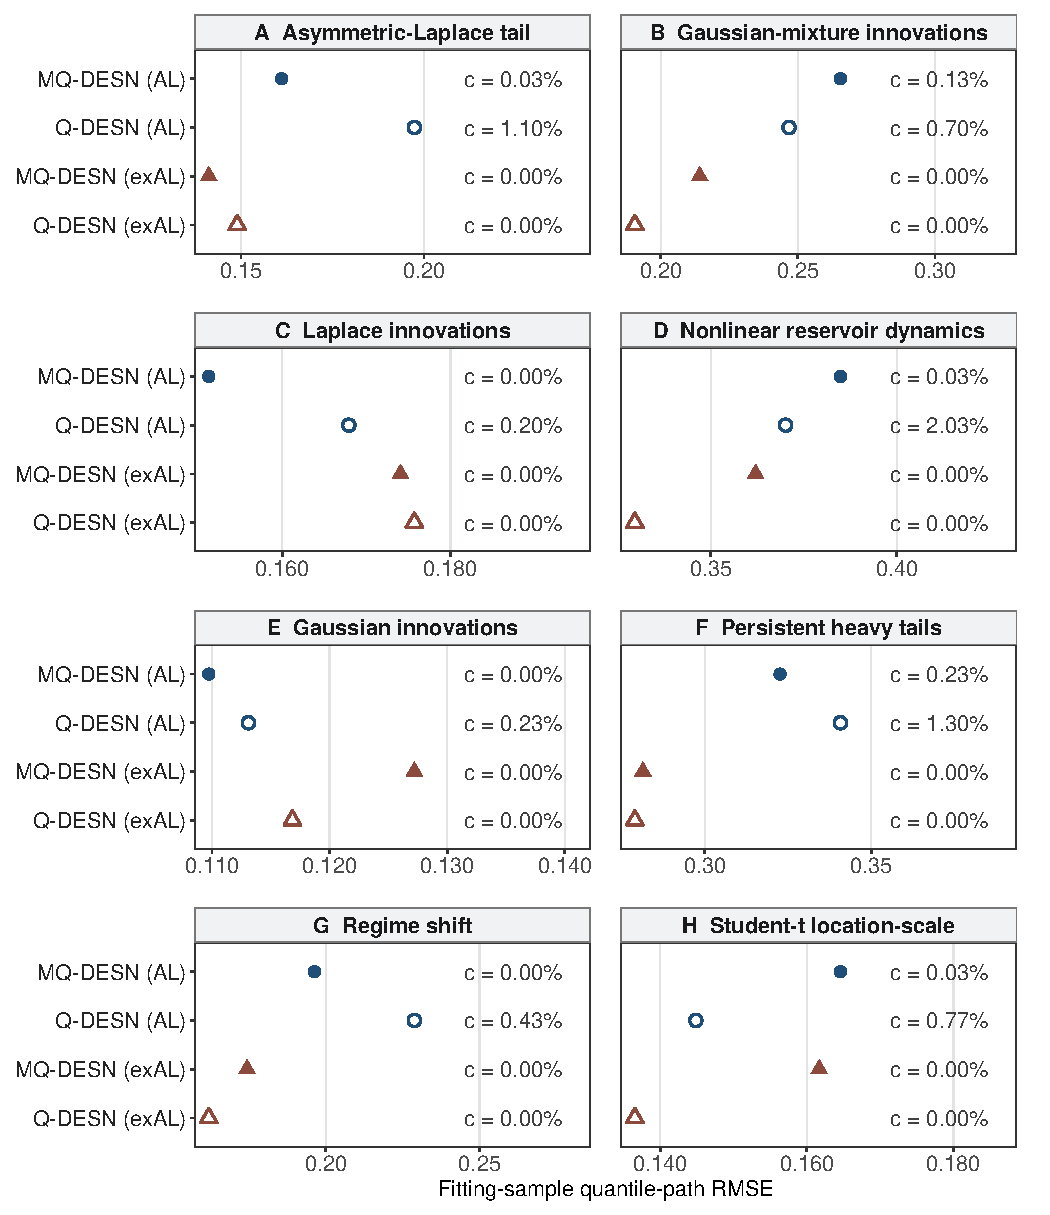
\includegraphics[width=0.94\textwidth]{figures/ch04-qdesn/joint_qdesn_simulation/joint_qdesn_pure_desn_v2_mq_fit_oracle_rmse.pdf}
\caption{Fitting-sample recovery of known conditional quantile paths in the multiquantile study. Points give the RMSE of monotone posterior-mean grids, not posterior interval summaries. Annotations \(c\) give raw adjacent-level crossing percentages before projection. Q--DESN fits levels independently; MQ--DESN estimates their coefficients jointly.}
\label{qdesn2026:fig:joint-qdesn-pure-desn-v2-fit-rmse}
\end{figure}

\begingroup
\footnotesize
\setlength{\tabcolsep}{3pt}
\renewcommand{\arraystretch}{1.08}
\begin{longtable}{@{}>{\raggedright\arraybackslash}p{0.21\textwidth}>{\raggedright\arraybackslash}p{0.15\textwidth}*{4}{>{\raggedleft\arraybackslash}p{0.12\textwidth}}@{}}
\caption{Recovery of known conditional quantile paths by projected posterior-mean grids. MAE and RMSE measure quantile-path recovery, separately from scores against observations. Fitting-sample entries are point summaries without posterior intervals. Q--DESN fits levels independently; MQ--DESN estimates their coefficients jointly.}\label{qdesn2026:tab:joint-qdesn-pure-desn-v2-oracle}\\
\toprule
Simulation setting & Model & Fit MAE & Fit RMSE & Forecast MAE & Forecast RMSE \\
\midrule
\endfirsthead
\caption[]{Continued.}\\
\toprule
Simulation setting & Model & Fit MAE & Fit RMSE & Forecast MAE & Forecast RMSE \\
\midrule
\endhead
\midrule
\multicolumn{6}{r}{\footnotesize Continued on next page}\\
\endfoot
\bottomrule
\endlastfoot
Asymmetric-Laplace tail & MQ--DESN (AL) & 0.1155 & 0.1611 & 0.1894 & 0.2373 \\
 & Q--DESN (AL) & 0.1397 & 0.1974 & 0.2793 & 0.3473 \\
 & MQ--DESN (exAL) & 0.1017 & 0.1412 & 0.1764 & 0.2376 \\
 & Q--DESN (exAL) & 0.1038 & 0.1489 & 0.3832 & 0.4911 \\
\addlinespace[2pt]
Gaussian-mixture innovations & MQ--DESN (AL) & 0.2114 & 0.2655 & 0.3272 & 0.4198 \\
 & Q--DESN (AL) & 0.1933 & 0.2468 & 0.2991 & 0.3827 \\
 & MQ--DESN (exAL) & 0.1722 & 0.2142 & 0.3245 & 0.4071 \\
 & Q--DESN (exAL) & 0.1513 & 0.1906 & 0.2646 & 0.3271 \\
\addlinespace[2pt]
Laplace innovations & MQ--DESN (AL) & 0.1188 & 0.1513 & 0.1500 & 0.1906 \\
 & Q--DESN (AL) & 0.1308 & 0.1679 & 0.1355 & 0.1690 \\
 & MQ--DESN (exAL) & 0.1376 & 0.1741 & 0.1808 & 0.2263 \\
 & Q--DESN (exAL) & 0.1395 & 0.1757 & 0.1699 & 0.2100 \\
\addlinespace[2pt]
Nonlinear reservoir dynamics & MQ--DESN (AL) & 0.3008 & 0.3849 & 0.2916 & 0.3683 \\
 & Q--DESN (AL) & 0.2895 & 0.3701 & 0.2447 & 0.3093 \\
 & MQ--DESN (exAL) & 0.2858 & 0.3621 & 0.3314 & 0.4162 \\
 & Q--DESN (exAL) & 0.2613 & 0.3296 & 0.2818 & 0.3569 \\
\addlinespace[2pt]
Gaussian innovations & MQ--DESN (AL) & 0.0884 & 0.1097 & 0.1563 & 0.1929 \\
 & Q--DESN (AL) & 0.0887 & 0.1131 & 0.2116 & 0.2471 \\
 & MQ--DESN (exAL) & 0.1062 & 0.1272 & 0.1881 & 0.2365 \\
 & Q--DESN (exAL) & 0.0939 & 0.1168 & 0.1959 & 0.2305 \\
\addlinespace[2pt]
Persistent heavy tails & MQ--DESN (AL) & 0.2428 & 0.3226 & 1.2793 & 1.6189 \\
 & Q--DESN (AL) & 0.2581 & 0.3408 & 1.1833 & 1.4584 \\
 & MQ--DESN (exAL) & 0.2103 & 0.2815 & 1.2248 & 1.5487 \\
 & Q--DESN (exAL) & 0.2102 & 0.2790 & 1.2073 & 1.4825 \\
\addlinespace[2pt]
Regime shift & MQ--DESN (AL) & 0.1527 & 0.1963 & 1.3994 & 1.6487 \\
 & Q--DESN (AL) & 0.1739 & 0.2288 & 1.2713 & 1.4642 \\
 & MQ--DESN (exAL) & 0.1376 & 0.1744 & 1.2539 & 1.4639 \\
 & Q--DESN (exAL) & 0.1269 & 0.1619 & 1.2135 & 1.3993 \\
\addlinespace[2pt]
Student-\(t\) location--scale & MQ--DESN (AL) & 0.1246 & 0.1646 & 0.1773 & 0.2193 \\
 & Q--DESN (AL) & 0.1053 & 0.1449 & 0.1680 & 0.2122 \\
 & MQ--DESN (exAL) & 0.1283 & 0.1617 & 0.2272 & 0.2719 \\
 & Q--DESN (exAL) & 0.1076 & 0.1365 & 0.2149 & 0.2567 \\
\end{longtable}
\endgroup


The comparison uses one recursive evaluation per mechanism. If
\(d_\beta\) denotes the number of penalized coefficients in an RHS
global-scale block, its conditional shape is \((d_\beta+1)/2\).
All four models use the same selected reservoir specification within
each scenario; their averaged future features may differ because their
simulated response trajectories differ.


\subsubsection{PriceFM Design and Additional Results}
\label{qdesn2026:subsec:supp_pricefm_diagnostics}

The PriceFM comparison evaluates average quantile loss (AQL) from independently
fitted quantile regressions and VB for 38 regions and three folds. Within each
region, reservoir and RHS-scale
selection uses three expanding temporal validation periods lying entirely
within the original Fold~1 training period. These validation periods are
September--December~2023, January--April~2024, and May--August~2024.
The outer Fold~1 validation period, September--December~2024, determines
the AL or exAL family. One specification is then held fixed across the three
test folds before scoring. There are no subsequent test-driven changes
or substitutions from the earlier case-specific comparison. The same periods
had been examined in that historical comparison; prospective selection here
refers to the present selection rule, not to previously unseen calendar
periods.

Table~\ref{qdesn2026:tab:supp-pricefm-fold-design} gives the outer validation and test
periods. Training begins on 1~January~2022 and ends at the start of each
validation period. All intervals are half-open. Dates use the released UTC
timestamps shifted by a fixed one hour, rather than a daylight-saving-aware
calendar. Each daily test origin has 96 quarter-hourly targets.

\begin{table}[!htbp]
\centering
\TableStyle
\caption{PriceFM outer validation and test periods. Training starts on
1~January~2022 and ends at the corresponding validation boundary. End dates
are excluded; target counts are per region.}
\label{qdesn2026:tab:supp-pricefm-fold-design}
\begin{tabular}{@{}cllr@{}}
\toprule
Fold & Validation period & Test period & Test targets \\
\midrule
1 & 2024-09-01 to 2025-01-01 & 2025-01-01 to 2025-05-01 & 11,520 \\
2 & 2025-01-01 to 2025-05-01 & 2025-05-01 to 2025-09-01 & 11,808 \\
3 & 2025-05-01 to 2025-09-01 & 2025-09-01 to 2026-01-01 & 11,712 \\
\bottomrule
\end{tabular}
\end{table}

The predictors use the released load, solar, and wind columns, identified
as day-ahead forecasts by \citet{qdesn-YuEtAl2026PriceFM}. Their availability at
each forecast origin was not separately verified, so the comparison does
not establish operational information parity. Selected spatial specifications either
concatenate neighboring-region predictors or add their means, with or
without standard deviations; other specifications use the target region
alone. Predictor and response scales are estimated separately using
training-only median and interquartile-range scaling. Selected lag windows
contain 48, 96, 168, or 240 quarter-hourly observations. All readouts use the
final reservoir layer and an intercept. The 38 selected specifications use
AL in 11 regions and exAL in 27.

The fixed-regional Q--DESN comparison has mean AQL 7.217, compared with
7.039 for PriceFM. Q--DESN is lower in
54 of 114 region--fold comparisons and in 16 of 38 region means. The fold-level
contrast changes sign: Q--DESN is slightly lower in fold~2, while PriceFM is
lower in folds~1 and 3. The largest mean loss difference occurs in fold~3,
while the aggregate remains slightly higher for Q--DESN. The former 72-case
forecast-lead summary is not reproduced because it does not cover all
114 comparisons under the fixed-regional specification.

\begin{table}[!htbp]
\centering
\caption{Aggregate AQL for the fixed-regional Q--DESN comparison, matched
PriceFM forecasts, and historical sensitivity. The historical Q--DESN result
uses earlier case-specific selection; it is not included in the primary
comparison and supplies no replacement cases. Lower values are better.}
\label{qdesn2026:tab:supp-pricefm-r98-global-comparison}
\begingroup
\TableStyle
\begin{tabular}{@{}lrr@{}}
\toprule
Comparison & Cases & Mean AQL \\
\midrule
Q--DESN (fixed regional specification) & 114 & 7.217007 \\
PriceFM & 114 & 7.038685 \\
Q--DESN (historical case-specific selection) & 114 & 6.823677 \\
\bottomrule
\end{tabular}
\endgroup

\end{table}

\begin{figure}[!htbp]
\centering
\includegraphics[width=\textwidth]{\PricefmCurrentRegionFigure}
\caption{Mean AQL across the three test folds for each PriceFM region. Blue
squares show Q--DESN with its fixed regional specification, green circles
show the matched PriceFM forecasts, and gray crosses show historical
case-specific Q--DESN results. Regions are ordered by increasing mean AQL
of the fixed-regional Q--DESN forecasts; lower values are better.}
\figalt{For each of 38 regions, the plot compares mean AQL across three folds
for fixed-regional Q--DESN, PriceFM, and historical case-specific Q--DESN.
The horizontal positions
show substantial regional heterogeneity, with PriceFM lower in 22 region means
and fixed-regional Q--DESN lower in 16.}
\label{qdesn2026:fig:supp-pricefm-r98-region-comparison}
\end{figure}


\subsection{GloFAS Reference--Discrepancy Forecast Correction}
\label{qdesn2026:sec:glofas_discrepancy}

The streamflow application combines the historical and issued Global Flood
Awareness System (GloFAS) products with a reference gauge record
\citep{qdesn-AlfieriEtAl2013GloFAS,qdesn-HarriganEtAl2023GloFASForecasts}. Separate DESN
feature maps represent the reference process and the GloFAS-minus-reference
discrepancy. Reference-only, discrepancy-only, and combined historical
regressions produce 30-day recursive paths. The issued-ensemble correction
instead uses 28 forecast horizons: future reference values are latent during
fitting, and the issued members contribute directly to the likelihood.
Each comparison includes Q--DESN and MQ--DESN under AL/exAL and two Gaussian
predictive baselines; the issued-window comparison also includes raw GloFAS.

\subsubsection{Observed Quantities and Latent Design}
\label{qdesn2026:subsec:glofas_aug_design}

The reference is daily streamflow measured by the United States Geological
Survey (USGS) at gauge 11160500 on the San Lorenzo
River at Big Trees, California. The historical GloFAS series is the v3.1
LISFLOOD consolidated product. Discharge values are expressed in
\(\mathrm{m}^3/\mathrm{s}\) before transformation. Let \(T\) denote
25~December~2022 and let \(y_t=\log(y_t^{\mathrm{USGS}}+1)\) be transformed
reference streamflow.
Write \(g_t^{\mathrm{ret}}\) for transformed retrospective GloFAS and
\(g_{T+h,e}^{\mathrm{ens}}\) for transformed issued member \(e\) at horizon
\(h\). The three historical models have a 30-day recursive horizon, ending
on 24~January~2023. For issued-ensemble correction, the latent future path
\(\vect y_F=(y_{T+1},\ldots,y_{T+28})^\top\) ends on 22~January~2023,
matching the available issued ensemble. All 51 members are used at each
horizon. The withheld USGS values are excluded from fitting and retained
separately for scoring. Forecast-period precipitation and soil-moisture
covariates use realized values from the Parameter-elevation Regressions on
Independent Slopes Model (PRISM) and the fifth-generation reanalysis (ERA5)
of the European Centre for Medium-Range Weather Forecasts (ECMWF). The
reference-only model retains 12,455 historical dates from
19~November~1988 through \(T\), after a 540-day initial-history exclusion.
The discrepancy-only design also contains 12,455 historical dates;
the combined historical model uses reference and retrospective-product
observations at those 12,455 dates, giving 24,910 stacked observations.

For probability level \(p_k\), the reference and source-specific
likelihood locations are
\begin{equation}
\begin{aligned}
\text{Reference quantile:}\quad
q_{k,t}
&=\vect x_t^{\mathrm{ref}\top}\vect\beta_k,\\
\text{Location adjustment:}\quad
d_{k,t}
&=\vect x_t^{\mathrm{disc}\top}\vect\delta_k,\\
\text{GloFAS quantile:}\quad
q_{k,t}^{\mathrm{glo}}
&=q_{k,t}+d_{k,t}.
\end{aligned}
\label{qdesn2026:eq:supp_glofas_quantile_decomposition}
\end{equation}
The additive relation specifies a quantile-indexed location adjustment;
it is not a general identity between the quantiles of a difference and
those of its two components. MQ--DESN links adjacent quantile-specific
coefficients separately within the reference and discrepancy components.
Historical reference features are generated from the observed reference
history, and historical discrepancy features are generated from
\(g_t^{\mathrm{ret}}-y_t\). After \(T\), the reference and discrepancy
reservoir states are recomputed as functions of the latent path
\(\vect y_F\). Strict lagging is imposed: the design row for \(T+h\) may
depend on earlier latent values but not on \(y_{T+h}\).

For one probability level, stack the reference and discrepancy coefficients as
\[
\vect\theta_k=
\begin{bmatrix}\vect\beta_k\\ \vect\delta_k\end{bmatrix},
\qquad
\vect h_t^{\mathrm{ref}}=
\begin{bmatrix}\vect x_t^{\mathrm{ref}}\\ \vect 0\end{bmatrix},
\qquad
\vect h_t^{\mathrm{glo}}=
\begin{bmatrix}\vect x_t^{\mathrm{ref}}\\
\vect x_t^{\mathrm{disc}}\end{bmatrix}.
\]
Then \(\vect h_t^{\mathrm{ref}\top}\vect\theta_k=q_{k,t}\) and
\(\vect h_t^{\mathrm{glo}\top}\vect\theta_k=q_{k,t}+d_{k,t}\).
Conditional on \(\vect y_F\), these are ordinary fixed-design Q--DESN
regressions.

\subsubsection{Historical Selection and Coefficient Priors}

Historical selection used 16 primary rainy-season development periods and
16 prespecified confirmation periods. Two additional periods in each group
were used to exclude candidates with excessive forecast deterioration.
Confirmation used four reservoir realizations to fix the reference and discrepancy
specifications.
The held-out December~2022--January~2023 forecast period was
not used to select reservoirs, priors, stopping rules, or model families.

The selected reference reservoir has depth one, width
\(\GlofasApplicationCurrentReferenceReservoirSize{}\), maximum response lag
\(\GlofasApplicationCurrentReferenceReservoirMemory{}\), leak rate
\(\GlofasApplicationCurrentReferenceReservoirAlpha{}\), spectral radius
\(\GlofasApplicationCurrentReferenceReservoirRho{}\), washout
\(\GlofasApplicationCurrentReferenceReservoirWashout{}\), and seed
\(\GlofasApplicationCurrentReferenceReservoirSeed{}\). Its inputs are reference
lags 1--540 and realized precipitation and soil-moisture lags 0--90. The
depth-one discrepancy reservoir has width
\(\GlofasApplicationCurrentDiscrepancyReservoirSize{}\), maximum response lag
\(\GlofasApplicationCurrentDiscrepancyReservoirMemory{}\), leak rate
\(\GlofasApplicationCurrentDiscrepancyReservoirAlpha{}\), spectral radius
\(\GlofasApplicationCurrentDiscrepancyReservoirRho{}\), washout
\(\GlofasApplicationCurrentDiscrepancyReservoirWashout{}\), and seed
\(\GlofasApplicationCurrentDiscrepancyReservoirSeed{}\). Its inputs are
discrepancy lags 1--180 and weather lags 0--180. Both maps standardize inputs
using training information and use a 500-observation washout. The readouts
contain reservoir features and intercepts, without direct response-lag or
weather regressors. Table~\ref{qdesn2026:tab:supp-glofas-search3-specifications}
summarizes the selected reservoir and prior specifications.

The training-based RHS calibration uses \(m_{0,\mathrm{ref}}=40\) and
\(m_{0,\mathrm{disc}}=60\), giving fixed prior hyperparameters
\(\tau_{0,\mathrm{ref}}=5.2043087445082\times10^{-5}\) and
\(\tau_{0,\mathrm{disc}}=1.1594362487914\times10^{-4}\) for the three
historical models.
The reference slab is learned under \(\zeta^2\sim\IG(2,4)\). The discrepancy
slab is fixed at \(\zeta^2=16\) for the discrepancy-only quantile regressions
and every discrepancy component of the combined historical model. The
discrepancy-only Gaussian DESN (RHS) baseline instead learns its slab under
\(\IG(2,4)\). The issued-ensemble RHS fits use
\(\tau_{0,\mathrm{ref}}=5.2043087\times10^{-5}\) and
\(\tau_{0,\mathrm{disc}}=1.159\times10^{-4}\), with learned
\(\IG(2,4)\) slabs for both components in every RHS family.
These \(\tau_0\) values are prior hyperparameters, not the learned global
scales. Posterior global scales vary by family, level, and adjacent-quantile
coefficient block. Table~\ref{qdesn2026:tab:supp-glofas-part123-priors} distinguishes
the fixed hyperparameters from these learned scales for the three
historical models.
Intercepts are exempt from RHS shrinkage.

The three historical Gaussian DESN (ridge) fits use coefficient prior variance
\(10^4\) and intercept variance \(10^6\). The issued-ensemble
Gaussian DESN (ridge) fit instead uses coefficient prior precision one and intercept
precision \(10^{-9}\). Table~\ref{qdesn2026:tab:supp-glofas-part4-priors} records the
issued-ensemble settings. Raw GloFAS has no fitted coefficient prior.

\begin{table}[!htbp]
\centering
\TableStyle
\caption{Reference and discrepancy specifications selected using historical
development and confirmation periods. Here \(m\) and \(m_x\) are the maximum
response and weather lags. Selection excludes the held-out final forecast
period. The slab column describes the selected prior; family-specific exceptions are
stated in the text.}
\label{qdesn2026:tab:supp-glofas-search3-specifications}
\input{\GlofasApplicationCurrentSpecificationsTable}
\end{table}

\begin{table}[!htbp]
\centering
\TableStyle
\caption{Prior settings for the reference-only, discrepancy-only, and combined
historical regressions, labeled Reference, Discrepancy, and Combined historical.
Fixed
RHS hyperparameters \(\tau_0\) are distinguished from the range of learned
effective global scales \(\{\E_q(\tau^{-2})\}^{-1/2}\) across quantile and
adjacent-quantile coefficient blocks. The discrepancy-only Gaussian DESN (RHS)
slab is learned; the other discrepancy-only slabs and all discrepancy slabs
in the combined historical model are fixed at 16. Gaussian DESN (ridge) has no RHS
global scale.}
\label{qdesn2026:tab:supp-glofas-part123-priors}
\input{\GlofasApplicationCurrentPartOneTwoThreePriorSettingsTable}
\end{table}

\begin{table}[!htbp]
\centering
\TableStyle
\caption{Issued-ensemble coefficient-prior settings. The two \(\tau_0\)
columns are fixed RHS hyperparameters, not learned posterior global scales.
All RHS families learn both slab scales under \(\IG(2,4)\); the Gaussian DESN (ridge)
and raw-ensemble baselines do not have RHS hyperparameters.}
\label{qdesn2026:tab:supp-glofas-part4-priors}
\input{\GlofasApplicationCurrentPriorSettingsTable}
\end{table}

\subsubsection{Weighted Augmented Likelihood}
\label{qdesn2026:subsec:glofas_likelihoods}

At each level \(p_k\), reference observations have AL location \(q_{k,t}\),
whereas retrospective and issued GloFAS observations have location
\(q_{k,t}+d_{k,t}\). Let \(z_i^c\) and \(\vect h_i^c\) denote an observation
and design row from source \(c\in\{\mathrm{ref},\mathrm{glo}\}\). The AL
normal--exponential augmentation is
\begin{equation}
\begin{aligned}
\text{Latent scale:}\quad
v_{i,k}^c\mid\sigma_{c,k}
&\sim\Exp(\mathrm{rate}=1/\sigma_{c,k}),\\
\text{Conditional observation:}\quad
z_i^c\mid\cdot
&\sim\Normal\!\left(
\vect h_i^{c\top}\vect\theta_k+A_{0,k}v_{i,k}^c,\,
\sigma_{c,k}B_{0,k}v_{i,k}^c
\right).
\end{aligned}
\label{qdesn2026:eq:supp_glofas_al_hierarchy}
\end{equation}

Define an observation weight \(w_i=1\) for historical reference and
retrospective GloFAS rows. For an issued member at a fixed horizon,
\(w_i=1/51\). Hence the 51 issued members contribute total weight one at each
horizon. The weighted augmented likelihood used for inference is
\begingroup\scriptsize\begin{equation}
\begin{aligned}
\text{Weighted augmented likelihood:}\quad
L_{\mathrm{aug}}(\Theta)
\ \propto\
\prod_{k=1}^{K}\prod_{c}\prod_{i\in\mathcal I_c}
\left[
p(z_i^c\mid v_{i,k}^c,\Theta_k)\,
p(v_{i,k}^c\mid\sigma_{c,k})
\right]^{w_i}.
\end{aligned}
\label{qdesn2026:eq:supp_glofas_weighted_augmented_likelihood}
\end{equation}\endgroup
This is a complete-data fractional or power-likelihood construction. It
prevents the issued ensemble from receiving 51 times the weight of one
historical time point. Because the power is applied before integrating out the
latent variables, Eq.~\eqref{qdesn2026:eq:supp_glofas_weighted_augmented_likelihood} is
not asserted to be an exact fractional marginal AL posterior.

The source-specific scales, coefficient priors, and latent variables are
updated under this weighted augmentation. The exAL comparator additionally
contains source-specific shape parameters and positive-shift latent variables,
using the structured quadrature calculations described earlier. Both AL and
exAL families are included in the final comparison.

\subsubsection{MQ--DESN and Latent-Path Approximation}
\label{qdesn2026:subsec:glofas_latent_path}

The fitted grid is
\[
(0.05,\ 0.20,\ 0.35,\ 0.50,\ 0.65,\ 0.80,\ 0.95).
\]
For the MQ--DESN families, the seven reference coefficient blocks and seven
discrepancy coefficient blocks are linked by separate adjacent-quantile RHS
priors. Computation uses mean-field quantile-block coordinate updates
initialized from the completed independent fits. The construction shares
information through these priors; it is not a single exact Gaussian update
over every coefficient and latent-path block. Independent families fit each
level separately.

The issued-ensemble quantile regressions use a Gaussian future-path prior
with mean and a numerically regularized covariance estimated from 500
recursive USGS paths from the combined historical Gaussian DESN (RHS) model,
restricted to the 28 issued horizons. Neither issued ensemble
values nor held-out USGS measurements enter its construction. Writing these moments
as \(\vect m_N\) and \(\mat V_N\), the prior is
\[
\text{Future-path prior:}\quad
\vect y_F\sim\Normal(\vect m_N,\mat V_N).
\]
This prior replaces, rather than supplements, a future-reference
likelihood. Issued-member contributions remain in the weighted augmented
likelihood. The Gaussian comparison families do not use this additional
path prior.

Each probability level has its own variational path factor; the following
notation suppresses the level index. At each coordinate update, the reservoir
design is linearized around the current path mean. Let
\(\widetilde\ell_F(\vect y_F)\) denote the resulting locally linearized
expected weighted augmented log likelihood plus the Gaussian log prior,
with the remaining variational factors held fixed. Its Gaussian factor has
mode \(\widehat{\vect y}_F\) and precision given by the negative Hessian of
this surrogate:
\begin{equation}
\begin{aligned}
\text{Latent-path factor:}\quad
\mat K_F&=-\nabla^2\widetilde\ell_F(\widehat{\vect y}_F),&
q_F(\vect y_F)&\approx
\Normal(\widehat{\vect y}_F,\mat K_F^{-1}).
\end{aligned}
\label{qdesn2026:eq:supp_glofas_future_path_factor}
\end{equation}
For design row \(\vect h_i^c(\vect y_F)\), let \(\mat J_i\) be its Jacobian at
the mode and \(\mat V_F=\mat K_F^{-1}\). The first-order moments propagated to
the remaining updates are
\begin{equation}
\begin{aligned}
\text{Propagated design moments:}\quad
\E\{\vect h_i^c(\vect y_F)\}
&\approx \vect a_i^c,\\
\E\{\vect h_i^c\vect h_i^{c\top}\}
&\approx \vect a_i^c\vect a_i^{c\top}
+\mat J_i\mat V_F\mat J_i^\top,
\end{aligned}
\label{qdesn2026:eq:supp_glofas_future_path_delta}
\end{equation}
where \(\vect a_i^c=\vect h_i^c(\widehat{\vect y}_F)\). The corresponding
Jacobian--covariance term is retained for cross-moments involving a component
of \(\vect y_F\). Repeated first-order updates give a local Gaussian--Delta
approximation, not an exact Laplace approximation to the nonlinear posterior.
Held-out USGS measurements do not enter the latent-path approximation,
and no post-hoc crossing correction is applied.

\subsubsection{Numerical Stopping and Supplementary Results}
\label{qdesn2026:subsec:glofas_checks}

Both MQ--DESN variational fits met the specified stopping criteria. The rule
requires every inner fit to meet its stopping criterion, outer parameter change below
\(10^{-3}\), relative change of every RHS block below \(10^{-3}\), and three
consecutive complete coordinate iterations meeting these tolerances after
global-scale updates begin. MQ--DESN (AL) met the criterion at outer iteration 11,
with parameter change
\(8.9279687\times10^{-4}\) and maximum RHS change
\(7.7748371\times10^{-4}\). MQ--DESN (exAL) met it at iteration 28, with
corresponding changes \(2.6080582\times10^{-4}\) and
\(3.8253514\times10^{-4}\). Table~\ref{qdesn2026:tab:supp-glofas-part4-convergence}
and Figure~\ref{qdesn2026:fig:supp-glofas-part4-convergence} report these results.
The structured exAL calculation retains the complete local variational state
between outer updates. Application inference is variational; no GloFAS MCMC
fit is reported.

Table~\ref{qdesn2026:tab:supp-glofas-part123-scores} separates the recursive evidence
from the issued-window comparison in Chapter~\ref{ch:research-c}. Reference-only and
combined historical forecasts are scored over 30 dates on the same
seven-level grid. Reference-only Q--DESN paths under AL and exAL contain
three and one adjacent-quantile crossing pairs, respectively. The
reference-only MQ--DESN paths and every combined historical forecast have
zero crossings. No correction was applied. All six post-cutoff discrepancy-only
paths are unscored because retrospective GloFAS ends at \(T\); their missing
scores and crossing counts are not zero-valued measurements.

Q--DESN under AL has the lowest descriptive issued-window score; this
ranking did not select a family using the held-out forecast period.
MQ--DESN (AL) is the multiquantile comparator and MQ--DESN (exAL) the sensitivity
model. The reported grids of all seven issued-ensemble families have zero
crossings. The nominal 90\% interval from Q--DESN under AL covers
\(0.750\) of the 28 outcomes; MQ--DESN (AL) has the
greatest modeled coverage, \(0.786\), still below nominal. At \(p=0.95\),
the empirical frequency below the MQ--DESN (exAL) forecast is only \(0.286\), compared
with \(0.750\) for Q--DESN (AL).
Table~\ref{qdesn2026:tab:supp-glofas-part4-calibration} and
Figure~\ref{qdesn2026:fig:supp-glofas-part4-calibration} show the substantial
disagreement with nominal frequencies across the grid.

\begin{figure}[!htbp]
\centering
\includegraphics[width=0.98\textwidth]{\GlofasApplicationCurrentFullComparisonFigure}
\caption{Full issued-ensemble forecast comparison. Panels group Gaussian and raw
GloFAS, Q--DESN, and MQ--DESN families; the separate
legend identifies probabilities and line styles. Black shows historical
USGS and magenta dashed lines show held-out measurements. The
vertical line marks 25 December 2022. Panels retain their original separate
vertical scales, unlike the common-scale illustration in Chapter~\ref{ch:research-c}.
All seven families and their unadjusted reported grids are retained.}
\figalt{The full issued-ensemble comparison retains Gaussian and raw GloFAS,
Q--DESN and MQ--DESN AL/exAL paths with their original panel scales,
historical observations, and held-out measurements.}
\label{qdesn2026:fig:supp-glofas-part4-all-families}
\end{figure}

\begin{table}[!htbp]
\centering
\TableStyle
\caption{Reference-only, discrepancy-only, and combined historical recursive
forecasts, labeled Reference, Discrepancy, and Combined historical, on the
\(\log(1+\mathrm{flow})\) scale and the seven-level probability grid.
Reference-only and combined historical models score 30 USGS horizons.
The discrepancy-only model supplies a 30-day path but has no future
retrospective-GloFAS observations and is unscored. Dashes
denote missing measurements by design. Crossing counts are adjacent-quantile
pairs over the raw paths, with no correction.}
\label{qdesn2026:tab:supp-glofas-part123-scores}
\input{\GlofasApplicationCurrentSupplementScoreTable}
\end{table}

\begin{table}[!htbp]
\centering
\TableStyle
\caption{Numerical stopping criteria for the issued-ensemble MQ--DESN fits. Both
parameter and maximum RHS relative changes are below \(10^{-3}\), all inner
fits meet their stopping criteria, and both families complete three consecutive
coordinate iterations meeting the stated tolerances after global-scale updates begin.}
\label{qdesn2026:tab:supp-glofas-part4-convergence}
\input{\GlofasApplicationCurrentConvergenceTable}
\end{table}

\begin{table}[!htbp]
\centering
\TableStyle
\caption{Issued-ensemble empirical quantile frequencies over the 28 horizons.
Entries are the fractions of held-out USGS observations below each fitted
quantile; the nominal frequency equals the column's probability level. All
families use the same dates and seven-level grid. This held-out-period
calibration assessment is descriptive, not a tuning criterion.}
\label{qdesn2026:tab:supp-glofas-part4-calibration}
\input{\GlofasApplicationCurrentCalibrationTable}
\end{table}

\begin{figure}[!htbp]
\centering
\includegraphics[width=0.98\textwidth]{\GlofasApplicationCurrentPartOneFigure}
\caption{Reference-only USGS recursive forecasts over 30 days after
25~December~2022. The three panels group Gaussian, independent quantile,
and MQ--DESN families. Colors distinguish probability levels and line
styles distinguish families. Black lines show the last 30 observed dates;
magenta dashed lines show held-out USGS measurements. Vertical lines mark
the origin and panels have separate vertical scales. Q--DESN under AL and
exAL has three and one raw crossing pairs, respectively; no correction is applied.}
\figalt{Three panels show 30-day reference-only USGS forecasts from Gaussian,
Q--DESN and MQ--DESN AL/exAL families, alongside black observed
history and magenta dashed held-out measurements.}
\label{qdesn2026:fig:supp-glofas-part1}
\end{figure}

\begin{figure}[!htbp]
\centering
\includegraphics[width=0.98\textwidth]{\GlofasApplicationCurrentPartTwoFigure}
\caption{Historical retrospective-GloFAS-minus-USGS discrepancy paths over the
last 30 observed dates and 30 recursive future dates. The discrepancy is
\(\log(1+\mathrm{GloFAS\ flow})-\log(1+\mathrm{USGS\ flow})\).
Panels group Gaussian,
Q--DESN, and MQ--DESN families, with color identifying probability levels
and line style identifying families. Gaussian paths are mean summaries.
Black lines show historical discrepancies and vertical lines mark the cutoff.
No future discrepancy observations are plotted or scored because retrospective GloFAS ends at
the cutoff; panels have separate vertical scales.}
\figalt{Three panels show historical black discrepancy lines and 30-day
future discrepancy paths for Gaussian and AL/exAL families. There are no
post-cutoff discrepancy observations or scores.}
\label{qdesn2026:fig:supp-glofas-part2}
\end{figure}

\begin{figure}[!htbp]
\centering
\includegraphics[width=0.98\textwidth]{\GlofasApplicationCurrentPartThreeFigure}
\caption{USGS recursive forecasts from the combined historical
reference--discrepancy model over 30 future dates. Gaussian, independent,
and MQ--DESN families occupy separate panels. Colors identify
probability levels, line styles identify families, and vertical lines mark
the December-25 origin. Black historical USGS and magenta dashed held-out
measurements accompany the forecasts. Panels have separate vertical scales. All
combined historical paths have zero crossings without correction.}
\figalt{Three family-group panels compare 30-day combined historical USGS quantile
forecasts with historical USGS and held-out measurements; all paths are uncrossed.}
\label{qdesn2026:fig:supp-glofas-part3}
\end{figure}

\begin{figure}[!htbp]
\centering
\includegraphics[width=0.98\textwidth]{\GlofasApplicationCurrentConvergenceFigure}
\caption{Numerical stopping for the issued-ensemble MQ--DESN fits. Maximum relative
parameter change is plotted against cumulative outer iteration on a
logarithmic vertical scale. The horizontal dashed line is the \(10^{-3}\)
outer tolerance. Triangles identify complete coordinate iterations meeting
the stopping criteria; the last three consecutive such iterations satisfy
the stopping rule for MQ--DESN (AL) and MQ--DESN (exAL).}
\figalt{Green MQ--DESN (AL) and brown MQ--DESN (exAL) parameter-change traces finish
below the specified tolerance at outer iterations 11 and 28, respectively,
with three consecutive coordinate iterations satisfying the stopping rule.}
\label{qdesn2026:fig:supp-glofas-part4-convergence}
\end{figure}

\begin{figure}[!htbp]
\centering
\includegraphics[width=0.98\textwidth]{\GlofasApplicationCurrentCalibrationFigure}
\caption{Issued-window empirical quantile frequencies. Colored lines give
the fraction of observations below each fitted quantile for the seven families;
the diagonal gives the nominal frequency. The comparison uses 28 held-out USGS
outcomes and was not used for model selection. Q--DESN under AL has the lowest
grid score but remains undercovered, and MQ--DESN (exAL) has
particularly low frequencies below its upper quantiles.}
\figalt{Seven empirical-frequency curves lie below the nominal diagonal.
MQ--DESN (AL) and Q--DESN (AL) have the highest frequency at p=0.95, while MQ--DESN
(exAL) reaches only 0.286 and raw GloFAS remains at zero.}
\label{qdesn2026:fig:supp-glofas-part4-calibration}
\end{figure}


\section{Gaussian baseline and initialization details}
\subsection{Scope and Relation to Q--DESN}
\label{qdesn2026:gauss:sec:scope}

After reservoir construction, spectral scaling, layer reduction, and washout,
the DESN feature map is fixed. Posterior inference for the readout is therefore
conditional on a deterministic design matrix
\(\mat X=[\vect x_1^\top;\ldots;\vect x_T^\top]\). The Gaussian DESN considered
in this note replaces the AL or exAL working likelihood with the homoskedastic
Normal likelihood
\begin{equation}
\label{qdesn2026:gauss:eq:gaussian_likelihood_scope}
\vect y\mid \vect\beta,\omega^2,\mat X
\sim \Normal_T(\mat X\vect\beta,\omega^2\mat I_T),
\qquad \omega^2>0.
\end{equation}
The variance parameter is denoted by \(\omega^2\), not \(\sigma\), to avoid
confusion with the AL/exAL scale parameter in Q--DESN.

The Gaussian DESN is not a quantile model. If the Gaussian likelihood is taken
literally, \(\vect x_t^\top\vect\beta\) targets a conditional mean under
squared-error loss. In Q--DESN, by contrast, \(\vect x_t^\top\vect\beta\) is the
conditional \(p_0\)-quantile under an AL or exAL working likelihood. The role of
this note is therefore computational:
\begin{enumerate}[label=(\roman*)]
\item provide an exact mean-regression baseline on the same fixed DESN features;
\item provide a conditioning and regularization diagnostic for the readout;
\item provide stable initial values for AL and exAL Q--DESN algorithms;
\item avoid unnecessary approximate inference for a model whose posterior is
available analytically.
\end{enumerate}

\subsection{Fixed DESN Design and Notation}
\label{qdesn2026:gauss:sec:fixed_design}

Let
\begin{equation}
\label{qdesn2026:gauss:eq:y_X_beta_dimensions}
\vect y=(y_1,\ldots,y_T)^\top\in\R^T,
\qquad
\mat X=[\vect x_1^\top;\ldots;\vect x_T^\top]\in\R^{T\times d},
\qquad d=r+1.
\end{equation}
Each row vector \(\vect x_t=(1,\tilde{\vect x}_t^\top)^\top\in\R^d\) contains
an intercept and \(r\) fixed DESN readout features. The coefficient vector is
partitioned as
\begin{equation}
\label{qdesn2026:gauss:eq:beta_partition}
\vect\beta=(\beta_0,\beta_1,\ldots,\beta_r)^\top\in\R^d,
\qquad
\vect\beta_{1:r}=(\beta_1,\ldots,\beta_r)^\top.
\end{equation}
The first coefficient is the intercept. The remaining \(r\) coefficients are
slopes associated with the fixed DESN features. No reservoir weight, input
weight, reducer, leak rate, or spectral-radius parameter is inferred in this
Gaussian readout.

For any \(\vect\beta\), define
\begin{equation}
\label{qdesn2026:gauss:eq:residuals}
\vect e(\vect\beta)=\vect y-\mat X\vect\beta,
\qquad
S_y(\vect\beta)=\|\vect y-\mat X\vect\beta\|^2.
\end{equation}
The identity matrix of size \(m\) is \(\mat I_m\).

\subsection{Distributional Conventions}
\label{qdesn2026:gauss:sec:dist_conventions}

All inverse-gamma distributions use the reciprocal-scale rate parameterization
\begin{equation}
\label{qdesn2026:gauss:eq:ig_density}
p(x\mid a,b)=\frac{b^a}{\Gamma(a)}x^{-a-1}\exp(-b/x),
\qquad x>0,
\end{equation}
written \(x\sim\IG(a,b)\). If \(x\sim\IG(a,b)\), then
\begin{equation}
\label{qdesn2026:gauss:eq:ig_moments}
\E(x^{-1})=\frac{a}{b},
\qquad
\E(x)=\frac{b}{a-1}\quad(a>1),
\qquad
\E(\log x)=\log b-\psi(a),
\end{equation}
where \(\psi(\cdot)\) is the digamma function. For a Gaussian factor,
\begin{equation}
\label{qdesn2026:gauss:eq:normal_entropy}
H\{\Normal_d(\vect m,\mat S)\}
=\frac12\{d(1+\log 2\pi)+\log|\mat S|\}.
\end{equation}
The notation \(\StudentT_\nu(\vect m,\mat S)\) denotes a multivariate Student
\(t\) distribution with degrees of freedom \(\nu\), location \(\vect m\), and
scale matrix \(\mat S\). Its covariance is \(\nu(\nu-2)^{-1}\mat S\), for
\(\nu>2\).

\subsection{Exact Scaled-Ridge Gaussian DESN}
\label{qdesn2026:gauss:sec:scaled_ridge}

\subsubsection{Model}
\label{qdesn2026:gauss:subsec:model}

The exact Gaussian baseline uses the conjugate scaled ridge prior
\begingroup\scriptsize\begin{align}
\vect y\mid\vect\beta,\omega^2,\mat X
&\sim \Normal_T(\mat X\vect\beta,\omega^2\mat I_T),
\label{qdesn2026:gauss:eq:likelihood}\\
\vect\beta\mid\omega^2
&\sim \Normal_d(\vect b,\omega^2\mat P^{-1}),
\label{qdesn2026:gauss:eq:scaled_prior}\\
\omega^2&\sim\IG(a_\omega,b_\omega),
\label{qdesn2026:gauss:eq:omega_prior}
\end{align}\endgroup
where \(a_\omega,b_\omega>0\), \(\mat P\in\R^{d\times d}\) is positive
definite, and
\begin{equation}
\label{qdesn2026:gauss:eq:b_P_definition}
\vect b=(b_0,0,\ldots,0)^\top,
\qquad
\mat P=\diag(P_0,\kappa_\beta^{-2},\ldots,\kappa_\beta^{-2}).
\end{equation}
If
\(\beta_0\mid\omega^2\sim\Normal(b_0,\omega^2V_0)\), then
\(P_0=V_0^{-1}\). More general positive definite \(\mat P\) can be used without
changing the derivation.

The scaling by \(\omega^2\) in \eqref{qdesn2026:gauss:eq:scaled_prior} is the key conjugacy
condition. It is not identical to an independent ridge prior
\(\vect\beta\sim\Normal_d(\vect b,\mat P^{-1})\). The scaled version is retained
here because it yields an exact one-shot posterior and is used only as a
baseline and initialization device for Q--DESN.

\subsubsection{Full joint distribution}
\label{qdesn2026:gauss:subsec:joint}

The joint density factors as
\begin{equation}
\label{qdesn2026:gauss:eq:joint_factorization}
p(\vect y,\vect\beta,\omega^2\mid\mat X)
=p(\vect y\mid\vect\beta,\omega^2,\mat X)
 p(\vect\beta\mid\omega^2)p(\omega^2).
\end{equation}
Writing all terms that depend on unknowns,
\begingroup\scriptsize\begin{align}
\label{qdesn2026:gauss:eq:joint_density_explicit}
p(\vect y,\vect\beta,\omega^2\mid\mat X)
&=(2\pi\omega^2)^{-T/2}
\exp\left\{-\frac{1}{2\omega^2}
(\vect y-\mat X\vect\beta)^\top(\vect y-\mat X\vect\beta)\right\}
\nonumber\\
&\quad\times
(2\pi\omega^2)^{-d/2}|\mat P|^{1/2}
\exp\left\{-\frac{1}{2\omega^2}
(\vect\beta-\vect b)^\top\mat P(\vect\beta-\vect b)\right\}
\nonumber\\
&\quad\times
\frac{b_\omega^{a_\omega}}{\Gamma(a_\omega)}
(\omega^2)^{-a_\omega-1}\exp(-b_\omega/\omega^2).
\end{align}\endgroup
Equivalently, up to constants independent of \((\vect\beta,\omega^2)\),
\begingroup\scriptsize\begin{align}
\label{qdesn2026:gauss:eq:log_joint}
\log p(\vect y,\vect\beta,\omega^2\mid\mat X)
&=\frac12\log|\mat P|+a_\omega\log b_\omega-\log\Gamma(a_\omega)
\nonumber\\
&\quad
-\left(a_\omega+1+\frac{T+d}{2}\right)\log\omega^2
\nonumber\\
&\quad
-\frac{1}{2\omega^2}\left[
\|\vect y-\mat X\vect\beta\|^2
+(\vect\beta-\vect b)^\top\mat P(\vect\beta-\vect b)
+2b_\omega\right].
\end{align}\endgroup

\subsubsection{Completing the square}
\label{qdesn2026:gauss:subsec:complete_square}

Define
\begingroup\scriptsize\begin{align}
\mat P_n&=\mat P+\mat X^\top\mat X,
\label{qdesn2026:gauss:eq:Pn}\\
\vect h_n&=\mat P\vect b+\mat X^\top\vect y,
\label{qdesn2026:gauss:eq:hn}\\
\vect m_n&=\mat P_n^{-1}\vect h_n,
\label{qdesn2026:gauss:eq:mn}\\
a_n&=a_\omega+\frac{T}{2},
\label{qdesn2026:gauss:eq:an}\\
B_n&=b_\omega+\frac12\left(
\vect y^\top\vect y+
\vect b^\top\mat P\vect b-
\vect m_n^\top\mat P_n\vect m_n
\right).
\label{qdesn2026:gauss:eq:Bn}
\end{align}\endgroup
Then
\begingroup\scriptsize\begin{align}
\label{qdesn2026:gauss:eq:complete_square_identity}
&\|\vect y-\mat X\vect\beta\|^2
+(\vect\beta-\vect b)^\top\mat P(\vect\beta-\vect b)
\nonumber\\
&\qquad=
(\vect\beta-\vect m_n)^\top\mat P_n(\vect\beta-\vect m_n)
+\vect y^\top\vect y+
\vect b^\top\mat P\vect b-
\vect m_n^\top\mat P_n\vect m_n.
\end{align}\endgroup
Substituting \eqref{qdesn2026:gauss:eq:complete_square_identity} into the joint density gives
an exact Normal--inverse-gamma posterior.

\subsubsection{Exact posterior}
\label{qdesn2026:gauss:subsec:exact_posterior}

The posterior factorization is
\begingroup\scriptsize\begin{align}
\omega^2\mid\vect y,\mat X&\sim\IG(a_n,B_n),
\label{qdesn2026:gauss:eq:omega_posterior}\\
\vect\beta\mid\omega^2,\vect y,\mat X
&\sim\Normal_d(\vect m_n,\omega^2\mat P_n^{-1}).
\label{qdesn2026:gauss:eq:beta_cond_posterior}
\end{align}\endgroup
Equivalently,
\begin{equation}
\label{qdesn2026:gauss:eq:joint_posterior_kernel}
p(\vect\beta,\omega^2\mid\vect y,\mat X)
=p(\vect\beta\mid\omega^2,\vect y,\mat X)p(\omega^2\mid\vect y,\mat X).
\end{equation}
The marginal coefficient posterior is multivariate Student \(t\):
\begin{equation}
\label{qdesn2026:gauss:eq:beta_student_posterior}
\vect\beta\mid\vect y,\mat X
\sim
\StudentT_{2a_n}\left(\vect m_n,\frac{B_n}{a_n}\mat P_n^{-1}\right).
\end{equation}
Hence
\begingroup\scriptsize\begin{align}
\E(\vect\beta\mid\vect y,\mat X)&=\vect m_n,
\label{qdesn2026:gauss:eq:posterior_mean_beta}\\
\Var(\vect\beta\mid\vect y,\mat X)
&=\frac{B_n}{a_n-1}\mat P_n^{-1},
\qquad a_n>1,
\label{qdesn2026:gauss:eq:posterior_var_beta}\\
\E(\omega^2\mid\vect y,\mat X)&=\frac{B_n}{a_n-1},
\qquad a_n>1.
\label{qdesn2026:gauss:eq:posterior_mean_omega}
\end{align}\endgroup
The posterior mode of \(\vect\beta\) and its posterior mean coincide at
\(\vect m_n\), while the marginal posterior for \(\vect\beta\) carries the
additional uncertainty induced by integrating out \(\omega^2\).

\subsection{Posterior Predictive Distributions}
\label{qdesn2026:gauss:sec:predictive}

For a new fixed DESN feature vector \(\vect x_*\in\R^d\), the posterior
predictive distribution is
\begin{equation}
\label{qdesn2026:gauss:eq:predictive_univariate}
y_*\mid\vect y,\mat X,\vect x_*
\sim
\StudentT_{2a_n}\left(
\vect x_*^\top\vect m_n,
\frac{B_n}{a_n}\{1+\vect x_*^\top\mat P_n^{-1}\vect x_*\}
\right).
\end{equation}
More generally, for a fixed future design matrix \(\mat X_*\in\R^{H\times d}\),
\begin{equation}
\label{qdesn2026:gauss:eq:predictive_multivariate}
\vect y_*\mid\vect y,\mat X,\mat X_*
\sim
\StudentT_{2a_n}\left(
\mat X_*\vect m_n,
\frac{B_n}{a_n}\{\mat I_H+\mat X_*\mat P_n^{-1}\mat X_*^\top\}
\right).
\end{equation}
The fixed-design condition matters. In multi-step DESN forecasting, future
features may depend on previously simulated responses. Conditional on any
particular generated feature path, \eqref{qdesn2026:gauss:eq:predictive_multivariate} applies.
If the feature path is recursively simulated, posterior prediction should
propagate draws through the reservoir recursion rather than treating
\(\mat X_*\) as known in advance.

\subsection{Exact Log Marginal Likelihood}
\label{qdesn2026:gauss:sec:log_marginal}

Integrating out both \(\vect\beta\) and \(\omega^2\) gives the closed-form
marginal likelihood
\begingroup\scriptsize\begin{align}
\label{qdesn2026:gauss:eq:log_marginal}
\log p(\vect y\mid\mat X)
&=-\frac{T}{2}\log(2\pi)
+\frac12\log|\mat P|-\frac12\log|\mat P_n|
+a_\omega\log b_\omega-a_n\log B_n
\nonumber\\
&\quad+\log\Gamma(a_n)-\log\Gamma(a_\omega).
\end{align}\endgroup
This replaces any need for an ELBO in the Gaussian baseline. It is also a
strong implementation check: exact posterior samplers and numerical posterior
summaries should be consistent with \eqref{qdesn2026:gauss:eq:log_marginal} and
\eqref{qdesn2026:gauss:eq:omega_posterior}--\eqref{qdesn2026:gauss:eq:beta_student_posterior}.

\subsection{Exact Direct Posterior Sampler}
\label{qdesn2026:gauss:sec:direct_sampler}

Because the posterior is available exactly, no Markov chain is required.
Independent posterior draws are generated directly as follows.

\begin{algorithmblock}{Direct sampler for the exact scaled-ridge Gaussian DESN}
\label{qdesn2026:gauss:alg:direct_sampler}
\emph{Input:} fixed design \(\mat X\), response \(\vect y\), prior
\((\vect b,\mat P,a_\omega,b_\omega)\), and desired number of draws \(M\).
\begin{enumerate}[label=(\arabic*)]
\item Compute \(\mat P_n\), \(\vect m_n\), \(a_n\), and \(B_n\) from
\eqref{qdesn2026:gauss:eq:Pn}--\eqref{qdesn2026:gauss:eq:Bn}.
\item For \(m=1,\ldots,M\):
  \begin{enumerate}[label=(\alph*)]
  \item draw \(\omega^{2(m)}\sim\IG(a_n,B_n)\);
  \item draw
  \(\vect\beta^{(m)}\mid\omega^{2(m)}
  \sim\Normal_d(\vect m_n,\omega^{2(m)}\mat P_n^{-1})\).
  \end{enumerate}
\item For fixed future \(\mat X_*\), optionally draw
\(\vect y_*^{(m)}\sim\Normal_H(\mat X_*\vect\beta^{(m)},
\omega^{2(m)}\mat I_H)\), or use the analytic Student distribution in
\eqref{qdesn2026:gauss:eq:predictive_multivariate}.
\end{enumerate}
\end{algorithmblock}

Algorithm~\ref{qdesn2026:gauss:alg:direct_sampler} is a direct posterior sampler, not a Gibbs
sampler. A Gibbs sampler would only reproduce a posterior that is already
available in closed form. Similarly, CAVI/VB would only approximate an exact
posterior. For this reason, Gibbs, CAVI, and ELBO derivations are intentionally
omitted from the main Gaussian baseline.

\subsection{Use as Initialization for AL and exAL Q--DESN}
\label{qdesn2026:gauss:sec:initialization}

The posterior mean \(\vect m_n\) gives a stable Gaussian readout estimate on the
same fixed DESN features used by Q--DESN. For a target quantile level
\(p_0\in(0,1)\), use it as a mean-regression warm start and then shift the
intercept to target the desired empirical quantile.

Define Gaussian residuals
\begin{equation}
\label{qdesn2026:gauss:eq:init_residuals}
r_t^N=y_t-\vect x_t^\top\vect m_n,
\qquad t=1,\ldots,T.
\end{equation}
Let
\begin{equation}
\label{qdesn2026:gauss:eq:empirical_resid_quantile}
c_{p_0}=\widehat Q_{p_0}(r_1^N,\ldots,r_T^N)
\end{equation}
be the empirical \(p_0\)-quantile of the Gaussian residuals. Set
\begingroup\scriptsize\begin{align}
\beta_0^{\mathrm{init}}(p_0)&=m_{n,0}+c_{p_0},
\label{qdesn2026:gauss:eq:init_beta0}\\
\beta_j^{\mathrm{init}}(p_0)&=m_{n,j},
\qquad j=1,\ldots,r.
\label{qdesn2026:gauss:eq:init_betaj}
\end{align}\endgroup
Then the empirical \(p_0\)-quantile of
\(y_t-\vect x_t^\top\vect\beta^{\mathrm{init}}(p_0)\) is approximately zero.
This makes \(\vect x_t^\top\vect\beta^{\mathrm{init}}(p_0)\) a more appropriate
initial quantile path than the raw Gaussian mean path.

With the check loss
\begin{equation}
\label{qdesn2026:gauss:eq:check_loss}
\rho_p(u)=u\{p-\ind(u<0)\},
\end{equation}
initialize the AL/exAL scale by
\begin{equation}
\label{qdesn2026:gauss:eq:init_sigma}
\sigma^{\mathrm{init}}
=\frac1T\sum_{t=1}^T
\rho_{p_0}\left(y_t-\vect x_t^\top\vect\beta^{\mathrm{init}}(p_0)\right)
+\epsilon,
\end{equation}
where \(\epsilon>0\) is a small numerical floor. For AL, no shape parameter or
\(s_t\) variables are used. For exAL, initialize at the AL special case,
\begin{equation}
\label{qdesn2026:gauss:eq:init_gamma}
\gamma^{\mathrm{init}}=0,
\end{equation}
or at a small jittered value near zero if the implementation uses an open
transformed support. Stable latent starts are
\begin{equation}
\label{qdesn2026:gauss:eq:init_latents}
v_t^{\mathrm{init}}=\sigma^{\mathrm{init}},
\qquad
s_t^{\mathrm{init}}=\sqrt{2/\pi}\quad\text{for exAL only}.
\end{equation}

For variational Q--DESN implementations, a Gaussian covariance scale can also
be initialized from
\begin{equation}
\label{qdesn2026:gauss:eq:init_covariance}
\widehat{\Var}(\vect\beta\mid\vect y,\mat X)
=\frac{B_n}{a_n-1}\mat P_n^{-1},
\qquad a_n>1,
\end{equation}
or from the conditional covariance
\(\widehat\omega^2\mat P_n^{-1}\) with
\(\widehat\omega^2=B_n/(a_n-1)\). These covariance quantities should be viewed
as numerical initializers rather than posterior uncertainty statements for the
AL/exAL quantile model.

\subsection{Omitted Variants and Why They Are Not Main Derivations}
\label{qdesn2026:gauss:sec:omitted_variants}

\subsubsection{Independent, unscaled ridge prior}
\label{qdesn2026:gauss:subsec:unscaled_omitted}

The independent ridge prior
\begin{equation}
\label{qdesn2026:gauss:eq:unscaled_prior_omitted}
\vect\beta\sim\Normal_d(\vect b,\mat P^{-1}),
\qquad
\omega^2\sim\IG(a_\omega,b_\omega)
\end{equation}
is conditionally conjugate: \(\vect\beta\mid\omega^2,\vect y,\mat X\) is
Gaussian and \(\omega^2\mid\vect\beta,\vect y,\mat X\) is inverse-gamma.
However, it does not yield the same one-shot Normal--inverse-gamma posterior as
Section~\ref{qdesn2026:gauss:sec:scaled_ridge}, because the coefficient prior is not scaled by
\(\omega^2\). It would require a Gibbs sampler or a mean-field approximation
for posterior computation. Since the purpose of this note is an exact Gaussian
baseline and initializer, the unscaled prior is not developed further here.

\subsubsection{Regularized horseshoe readout prior}
\label{qdesn2026:gauss:subsec:rhs_omitted}

A Gaussian DESN with the Nishimura--Suchard regularized-horseshoe
\texttt{rhs\_ns} prior is also conditionally conjugate under its product
representation. Given the local, global, and slab scales, the coefficient block
is Gaussian, and the scale blocks can have inverse-gamma updates. Nevertheless,
after integrating over those shrinkage scales, the marginal posterior is not a
single closed-form Normal--inverse-gamma or Student distribution. Thus the
\texttt{rhs\_ns} Gaussian model is useful as a conditional Gibbs or CAVI warm
start, but it is not the exact closed-form baseline derived in this note.

For Q--DESN initialization, the recommended default is therefore
\begin{equation}
\label{qdesn2026:gauss:eq:init_pipeline}
\begin{gathered}
\text{exact scaled-ridge Gaussian DESN}\\
\longrightarrow\ \text{quantile-shifted }\vect\beta^{\mathrm{init}}(p_0)\\
\longrightarrow\ \text{AL/exAL Q--DESN}.
\end{gathered}
\end{equation}
If adaptive RHS shrinkage is required in the final Q--DESN fit, RHS scale
initializations can still be constructed from the shifted ridge coefficients,
for example
\begingroup\scriptsize\begin{align}
\tau^{\mathrm{init}}
&=\operatorname{median}_{j=1,\ldots,r}|\beta_j^{\mathrm{init}}|+
\epsilon,
\label{qdesn2026:gauss:eq:init_tau_rhs}\\
\lambda_j^{\mathrm{init}}
&=\max\left\{\lambda_{\min},
\frac{|\beta_j^{\mathrm{init}}|}{\tau^{\mathrm{init}}}\right\},
\qquad j=1,\ldots,r,
\label{qdesn2026:gauss:eq:init_lambda_rhs}\\
\zeta^{\mathrm{init}}
&=\max_{j=1,\ldots,r}|\beta_j^{\mathrm{init}}|+
\epsilon.
\label{qdesn2026:gauss:eq:init_zeta_rhs}
\end{align}\endgroup
These are initialization heuristics, not an exact RHS posterior calculation.

\subsection{Implementation Notes}
\label{qdesn2026:gauss:sec:implementation}

The main computational object is the positive definite precision matrix
\(\mat P_n=\mat P+\mat X^\top\mat X\). Implementations should use Cholesky
factorization of \(\mat P_n\) for all solves, log determinants, and Gaussian
sampling. Avoid explicit matrix inversion except in small diagnostic scripts.
For example,
\begin{equation}
\label{qdesn2026:gauss:eq:solve_not_inverse}
\vect m_n=\mat P_n^{-1}\vect h_n
\end{equation}
should be computed by solving \(\mat P_n\vect m_n=\vect h_n\).

For the log marginal likelihood,
\(\log|\mat P_n|\) and \(\log|\mat P|\) should be obtained from Cholesky factors.
For posterior covariance diagnostics, use triangular solves to compute selected
diagonal entries or linear-function variances rather than forming a dense
inverse when \(d\) is large.

Feature preprocessing should be fixed before inference. Centering and scaling
non-intercept DESN features can improve conditioning, but the intercept column
should remain an explicit column of ones. The prior precision \(P_0\) controls
intercept regularization separately from the slope precision
\(\kappa_\beta^{-2}\).

\subsection{Validation and Consistency Checks}
\label{qdesn2026:gauss:sec:validation}

\subsubsection{Dimension checks}

\begin{enumerate}[label=(\alph*)]
\item \(\mat X\in\R^{T\times d}\), \(\mat X^\top\mat X\in\R^{d\times d}\),
\(\mat P\in\R^{d\times d}\), and \(\mat P_n\in\R^{d\times d}\).
\item \(\vect h_n=\mat P\vect b+\mat X^\top\vect y\in\R^d\), hence
\(\vect m_n\in\R^d\).
\item \(B_n\) is scalar and positive when the prior is proper and
\(\mat P_n\) is positive definite.
\item \(\vect x_*^\top\mat P_n^{-1}\vect x_*\) is scalar and nonnegative.
\end{enumerate}

\subsubsection{Conjugacy checks}

\begin{enumerate}[label=(\alph*)]
\item The scaled prior contributes \(-d\log\omega^2/2\) to the joint density,
but this factor is canceled by the Gaussian integral over \(\vect\beta\) when
obtaining \(\omega^2\mid\vect y\). Therefore the marginal shape is
\(a_\omega+T/2\), not \(a_\omega+(T+d)/2\).
\item Conditional on \(\omega^2\), the posterior precision for \(\vect\beta\) is
\(\omega^{-2}\mat P_n\), and the posterior covariance is
\(\omega^2\mat P_n^{-1}\).
\item Integrating \(\omega^2\) gives the Student posterior in
\eqref{qdesn2026:gauss:eq:beta_student_posterior} with degrees of freedom \(2a_n\).
\item The posterior predictive variance includes both observation noise and
coefficient uncertainty through
\(1+\vect x_*^\top\mat P_n^{-1}\vect x_*\).
\end{enumerate}

\subsubsection{Numerical checks}

\begin{enumerate}[label=(\alph*)]
\item Independent draws from Algorithm~\ref{qdesn2026:gauss:alg:direct_sampler} should match
\(\E(\omega^2\mid\vect y,\mat X)=B_n/(a_n-1)\) and
\(\E(\vect\beta\mid\vect y,\mat X)=\vect m_n\), within Monte Carlo error.
\item The empirical covariance of sampled \(\vect\beta\) should match
\(B_n(a_n-1)^{-1}\mat P_n^{-1}\), for \(a_n>1\).
\item The direct Student sampler for \(\vect\beta\) and the two-step
\(\omega^2,\vect\beta\mid\omega^2\) sampler should give the same marginal
summaries.
\item The log determinant terms in \eqref{qdesn2026:gauss:eq:log_marginal} should be computed
from Cholesky factors and checked for finite values.
\item The condition numbers of \(\mat X^\top\mat X\), \(\mat P\), and
\(\mat P_n\) should be monitored. Poor conditioning indicates a feature-scaling
or reservoir-design issue, not a posterior-derivation issue.
\end{enumerate}

\subsubsection{Q--DESN initialization checks}

\begin{enumerate}[label=(\alph*)]
\item After the intercept shift in \eqref{qdesn2026:gauss:eq:init_beta0}, the empirical
\(p_0\)-quantile of
\(y_t-\vect x_t^\top\vect\beta^{\mathrm{init}}(p_0)\) should be close to zero.
\item The initialized AL/exAL scale in \eqref{qdesn2026:gauss:eq:init_sigma} must be strictly
positive.
\item The initialized exAL shape value must lie in the quantile-dependent
support \((L,U)\). If \(0\) is represented only as a boundary case in code, use
a small interior jitter around zero.
\item If RHS shrinkage scales are initialized by
\eqref{qdesn2026:gauss:eq:init_tau_rhs}--\eqref{qdesn2026:gauss:eq:init_zeta_rhs}, all scales must be finite and
positive.
\end{enumerate}

\subsubsection{Final self-audit}

This note keeps only the scaled-ridge Gaussian DESN as the main model because
it is the version with an exact closed-form posterior. It does not present
Gibbs, CAVI, or ELBO algorithms for the main model because those methods are
unnecessary approximations or redundant samplers for an analytically available
posterior. Unscaled ridge and \texttt{rhs\_ns} priors are described only to
clarify why they are not the exact baseline: both are useful conditionally
conjugate models, but neither yields the same one-shot closed-form marginal
posterior after all nuisance quantities are integrated out.

\chapter{Technical details for mean-preserving and mean-tilted intervals}
\label{app:mti-technical}

% migration-id: MIG-CH05-CURRENT-RQR
% migration-id: MIG-CH05-CURRENT-MTI-EXT
This appendix preserves the proofs, profile calculation, content checks, calibration protocol, application diagnostics, and proposed regression and dynamic computations supporting Chapter~\ref{ch:research-d}.

\section{Foundations, profiled computation, and validation details}
\subsection{Fixed-Content Interval Targets}
\label{rqr2026:sec:supp-interval-functionals}

The population interval class is most transparent on the probability scale.
Suppress \(x\) and write
\[
I_c(u)=[Q(u),Q(u+c)],\qquad
M_c(u)=\frac{1}{c}\int_u^{u+c}Q(v)\,dv,\qquad
W_c(u)=Q(u+c)-Q(u).
\]
The equal-tailed interval fixes \(u_{\mathrm{ET}}=(1-c)/2\). MPI
solves \(M_c(u_{\mathrm{MPI}})=\mu\). Define the possibly set-valued collection
of shortest contiguous windows by
\[
S_{\mathrm{SH}}
=\argmin_{0\le u\le1-c}W_c(u).
\]
If a positive density exists at an interior \(u_{\mathrm{SH}}\in
S_{\mathrm{SH}}\), then
\[
W_c'(u_{\mathrm{SH}})
=\frac{1}{f\{Q(u_{\mathrm{SH}}+c)\}}
-\frac{1}{f\{Q(u_{\mathrm{SH}})\}}=0,
\]
so the endpoint densities agree. For a continuous strictly unimodal density
and a unique regular shortest interval, this interval agrees with the
corresponding highest-density interval. Under multimodality, a highest-density
region can be disconnected; the present construction remains restricted to
one contiguous interval
\citep{rqr-BrehmerGneiting2021Intervals}.

Under a symmetric unimodal distribution, all three intervals coincide. Under
asymmetry, their widths need not coincide; only the shortest interval is
ordered against the other two by definition. The standard interval score is
aligned with the central equal-tailed target and is not a target-neutral score
for this comparison
\citep{exd-gneiting2007,rqr-BrehmerGneiting2021Intervals,rqr-FisslerEtAl2021SetValued}.

\subsection{Mean-Preserving Interval Scores}
\label{rqr2026:sec:supp-population-target}

The derivation starts from the endpoint scores because those scores determine
both content and placement. Fix a covariate value \(x\), a desired content
\(c\in(0,1)\), and endpoints
\(a=L(x)<U(x)=b\). The pointwise loss is
\begin{equation}
\ell_c(a,b;y)
=
\begin{cases}
(1-c)(y-a)(b-y), & a<y<b,\\
c(y-a)(y-b), & y\le a\ \text{or}\ y\ge b.
\end{cases}
\label{rqr2026:eq:supp-mpi-loss-piecewise}
\end{equation}
Equivalently, with
\(e(a,b;y)=(y-a)(y-b)\) and
\(\rho_c(r)=r\{c-\ind(r<0)\}\),
\begin{equation}
\ell_c(a,b;y)=\rho_c\{e(a,b;y)\}.
\label{rqr2026:eq:supp-mpi-product-check}
\end{equation}
The check function is applied to the product residual. Its index \(c\) denotes
the desired interval content rather than a prescribed response-quantile level
for either endpoint or a generalized-Bayes learning rate. The loss is symmetric
in its two roots; ordering is used only for the endpoint interpretation.

Define \(I_{a,b}(Y)=\ind(a<Y<b)\). Away from the two roots, the derivative of
the check loss with respect to its scalar argument is
\(c-I_{a,b}(Y)\). Assume
\(\E(Y^2\mid X=x)<\infty\), the conditional risk is differentiable at an
interior stationary point, differentiation and conditional expectation may be
interchanged, and the conditional distribution places no mass at \(a\) or
\(b\). Since
\[
\frac{\partial}{\partial a}(Y-a)(Y-b)=b-Y,
\qquad
\frac{\partial}{\partial b}(Y-a)(Y-b)=a-Y,
\]
the pointwise first-order conditions are
\begin{align}
\E\left[\{c-I_{a,b}(Y)\}(b-Y)\mid X=x\right]&=0,
\label{rqr2026:eq:pop-foc-a}\\
\E\left[\{c-I_{a,b}(Y)\}(a-Y)\mid X=x\right]&=0.
\label{rqr2026:eq:pop-foc-b}
\end{align}
Subtracting \eqref{rqr2026:eq:pop-foc-b} from \eqref{rqr2026:eq:pop-foc-a} and using
\(b-a>0\) gives
\[
\Pr\{a<Y<b\mid X=x\}=c.
\]
Substitution into either first-order condition then gives
\[
\E\{Y\ind(a<Y<b)\mid X=x\}=c\E(Y\mid X=x).
\]

The second equation is equivalently
\[
\E(Y\mid a<Y<b,X=x)=\E(Y\mid X=x)
\]
and
\(\operatorname{Cov}\{Y,I_{a,b}(Y)\mid X=x\}=0\). This covariance statement is
compatible with dependence, asymmetry, and unequal-tailed endpoints. The
coverage implication is established by \citet{rqr-PouplinEtAl2024RQR}; the
conditional first-moment implication is a further consequence of their
first-order system.

Let \(\mu_x=\E(Y\mid X=x)\). Since
\(\E(Y-\mu_x\mid X=x)=0\), the first-moment equation is also equivalent to
\begin{equation}
\E[\{\mu_x-Y\}\ind(Y<a)\mid X=x]
=
\E[\{Y-\mu_x\}\ind(Y>b)\mid X=x].
\label{rqr2026:eq:rqr-tail-moment-balance}
\end{equation}
Thus MPI balances omitted tail probability multiplied by average
tail displacement from the conditional mean. The two omitted tail probabilities
may differ.

\begin{theorem}[Quantile-window identification]
\label{rqr2026:thm:supp-quantile-window}
Suppose, in addition, that \(F_x\) is continuous and strictly increasing on
its support, and let \(Q_x=F_x^{-1}\). Define
\[
M_{c,x}(u)=\frac{1}{c}\int_u^{u+c}Q_x(v)\,dv,
\qquad 0\le u\le1-c.
\]
Then \(M_{c,x}\) is strictly increasing, and there is a unique \(u_c(x)\)
satisfying \(M_{c,x}\{u_c(x)\}=\mu_x\). The corresponding interval is
\[
\left[Q_x\{u_c(x)\},Q_x\{u_c(x)+c\}\right].
\]
\end{theorem}

\begin{proof}
Modulo conditional probability-zero portions outside the support, every
contiguous interval having content \(c\) has the displayed
quantile-window form. If \(v>u\), then
\[
M_{c,x}(v)-M_{c,x}(u)
=\frac{1}{c}\int_0^c
\{Q_x(v+s)-Q_x(u+s)\}\,ds>0.
\]
The average of the lowest conditional \(c\)-fraction is below \(\mu_x\), and
the average of the highest conditional \(c\)-fraction is above \(\mu_x\), for
a nondegenerate distribution with finite mean. Continuity and strict
monotonicity therefore give existence and uniqueness. The first-moment
equation identifies the stated endpoints.
\end{proof}

If \(F_x\) is symmetric about \(\mu_x\), then
\(Q_x(1-v)=2\mu_x-Q_x(v)\). The window beginning at
\((1-c)/2\) has retained mean \(\mu_x\), so uniqueness gives the equal-tailed
interval. Conversely, coincidence at one coverage level does not establish
global symmetry.

The distribution conditional on interval membership and its complementary
tail distribution both have mean \(\mu_x\). This is a first-moment statement,
not independence between \(Y\) and interval membership. It also clarifies why
the endpoint midpoint need not equal \(\mu_x\) under asymmetry.

\begin{proposition}[Mean-preserving contraction]
\label{rqr2026:prop:supp-convex-order}
Let \(Y_{\mathrm{in}}\) and \(Y_{\mathrm{out}}\) have the conditional
distributions of \(Y\) given \(a<Y<b\) and \(Y\notin(a,b)\), respectively,
at a regular MPI target. For every convex function \(\varphi\) for
which the required expectations exist,
\[
\E\{\varphi(Y_{\mathrm{in}})\}
\le
\E\{\varphi(Y)\}
\le
\E\{\varphi(Y_{\mathrm{out}})\}.
\]
Consequently,
\[
Y_{\mathrm{in}}\preceq_{\mathrm{cx}}Y
\preceq_{\mathrm{cx}}Y_{\mathrm{out}}.
\]
If second moments exist, the same ordering holds for the corresponding
variances.
\end{proposition}

\begin{proof}
Let \(s_\varphi\) be the affine secant through
\(\{a,\varphi(a)\}\) and \(\{b,\varphi(b)\}\). Convexity gives
\(\varphi(y)\le s_\varphi(y)\) on \([a,b]\) and
\(\varphi(y)\ge s_\varphi(y)\) outside that interval. Both conditional
distributions have mean \(\mu_x\), so
\[
\E\{\varphi(Y_{\mathrm{in}})\}
\le s_\varphi(\mu_x)
\le \E\{\varphi(Y_{\mathrm{out}})\}.
\]
The full conditional distribution is their mixture with weights \(c\) and
\(1-c\), which places its convex expectation between the two. Taking
\(\varphi(y)=(y-\mu_x)^2\) gives the variance statement.
\end{proof}

\subsubsection{Interval Paths and Tail Sensitivity}

Retain the quantile-window characterization and assume, for this derivative
calculation, connected support and positive continuous density at the relevant
endpoint quantiles. Write \(u_c\) for the MPI index, and set
\(L_c=Q(u_c)\) and \(U_c=Q(u_c+c)\). Differentiating
\[
\int_{u_c}^{u_c+c}\{Q(v)-\mu\}\,dv=0
\]
with respect to \(c\), at regular interior values, gives
\[
\frac{du_c}{dc}
=-\frac{U_c-\mu}{U_c-L_c}<0,
\qquad
\frac{d(u_c+c)}{dc}
=\frac{\mu-L_c}{U_c-L_c}>0.
\]
The MPI population intervals are therefore nested as content
increases, with analogous one-sided statements at isolated nonsmooth support
transitions. If \(p_\mu=F(\mu)\) satisfies \(Q(p_\mu)=\mu\) and \(Q\) is
continuous at \(p_\mu\), then \(Q(u_c)\le\mu\le Q(u_c+c)\), so
\(p_\mu\in[u_c,u_c+c]\). Since this probability window has length \(c\),
\[
L_c\longrightarrow\mu,\qquad U_c\longrightarrow\mu
\quad\text{as }c\downarrow0.
\]
This zero-content limit needs the local support condition above. It is false
under the quantile-window assumptions alone: for the symmetric distribution
with density \(1/2\) on \([-2,-1]\cup[1,2]\), \(\mu=0\) and the MPI
window has \(u_c=(1-c)/2\), hence \(L_c=-1-c\) and \(U_c=1+c\), so the
zero-content limit straddles the support gap rather than contracting to
\(\mu\). The corrected zero-content limit is a property of the population
interval path; the
midpoint at a fixed positive \(c\) is not generally the mean, and independent
fits at several content levels do not by themselves define joint
generalized-posterior draws of that path.

For \(Y^\star=r+sY\), \(s>0\), the MPI endpoints transform as
\[
L_c^\star=r+sL_c,\qquad U_c^\star=r+sU_c.
\]
For the tilted family, \(\delta^\star=s\delta\) and
\[
\ell^\star_{c,\delta^\star}
(r+sa,r+sb;r+sy)
=s^2\ell_{c,\delta}(a,b;y).
\]
Thus the population target is positive-affine equivariant. A corresponding
generalized posterior uses the transformed prior and
\(\omega_{\mathrm R}^\star=\omega_{\mathrm R}/s^2\). Conversely, if the
original response is standardized as \(\widetilde Y=(Y-r)/s\), use
\(\widetilde\delta=\delta/s\) and
\(\widetilde\omega_{\mathrm R}=\omega_{\mathrm R}s^2\).
Nonlinear monotone transformations generally change the mean-preserving
functional rather than merely re-expressing it.

Finally, with fixed endpoints,
\(\rho_c\{(y-a)(y-b)\}=O(y^2)\) as \(|y|\to\infty\), and the endpoint scores
grow linearly in \(|y|\). MPI is distribution-free in the sense that it does
not posit a parametric response density. Its retained-mean target still depends
on second moments, so the finite-second-moment assumption and response-scale
choice are scientifically consequential.

Endpoint atoms require directional conditions. Write
\(m=(a+b)/2\), \(h=(b-a)/2>0\), so
\(e=(Y-m)^2-h^2\). The left and right derivatives in \(h\) are
\[
D_-R_x(m,h)=2h\{\Pr(a<Y<b\mid x)-c\},
\]
and
\[
D_+R_x(m,h)=2h\{\Pr(a\le Y\le b\mid x)-c\}.
\]
At a local minimum, \(D_-R_x\le0\le D_+R_x\), and therefore
\[
\Pr(a<Y<b\mid X=x)\le c\le\Pr(a\le Y\le b\mid X=x).
\]
Without a separate joint subgradient and endpoint-mass allocation analysis,
these directional conditions do not imply the exact retained-mean equality
derived above under endpoint continuity.
If \(a=b=m\), then \(e=(Y-m)^2\) and the risk is
\(c\E\{(Y-m)^2\mid X=x\}\); the coincident-root target is the conditional
mean when the second moment exists.

These implications are conditional, pointwise, and assumption dependent. They
do not follow by treating estimated data-dependent endpoints as fixed. For
linear roots \(\eta_k(X)=X^\top\beta_k\), the corresponding population score
conditions are instead
\begin{align}
\E\left[X\{c-I_{\eta_1,\eta_2}(Y)\}(\eta_2-Y)\right]&=0,\\
\E\left[X\{c-I_{\eta_1,\eta_2}(Y)\}(\eta_1-Y)\right]&=0,
\end{align}
where \(I_{\eta_1,\eta_2}(Y)\) indicates that \(Y\) lies between the
unordered roots. These design-weighted projection equations need not imply
conditional coverage for every \(x\).

The finite-sample unbiasedness calculation in
\citet{rqr-PouplinEtAl2024RQR} treats fitted, data-dependent endpoints as fixed,
and its zero-gradient argument does not cover nonsmooth optima when an
observation coincides with a fitted root. We therefore do not use that
calculation as a finite-sample guarantee; such a result requires a separate
empirical-process analysis.

\subsection{Mean-Tilted Interval Loss and Target}
\label{rqr2026:sec:supp-mean-tilt}

The MTI loss is the fixed-tilt generalization of MPI. It keeps the MPI content
score and shifts only the retained-mean equation; setting \(\delta=0\) recovers
the MPI loss. For a fixed mean tilt \(\delta\in\R\), define
\begin{equation}
\ell_{c,\delta}^{\mathrm{MTI}}(m,h;y)
=\rho_c\{(y-m)^2-h^2\}-2c\delta(m-y),
\label{rqr2026:eq:mean-tilted-loss-midpoint}
\end{equation}
or, equivalently,
\begin{equation}
\ell_{c,\delta}^{\mathrm{MTI}}(a,b;y)
=\rho_c\{(y-a)(y-b)\}-c\delta(a+b-2y).
\label{rqr2026:eq:mean-tilted-loss-roots}
\end{equation}
The second form is invariant to exchanging the raw root labels. The tilt has
response units so that both terms in the loss have squared-response units, and
nonzero \(\delta\) changes the target placement rather than the content score.
For restricted linear roots \(\eta_k(X)=X^\top\beta_k\) and an externally
fixed \(\delta(X)\), the population score equations are
\begin{align}
\E\!\left[
X\left\{\{c-I_{\eta_1,\eta_2}(Y)\}(\eta_2-Y)-c\delta(X)\right\}
\right]&=0,\\
\E\!\left[
X\left\{\{c-I_{\eta_1,\eta_2}(Y)\}(\eta_1-Y)-c\delta(X)\right\}
\right]&=0.
\end{align}
They are design-weighted projection equations. Pointwise conditional content
and retained-mean identities require a sufficiently rich predictor class and
the unrestricted conditions below.

\subsubsection{Fixed-Content Mean-Tilted Target}

The next proposition records the population score equations supported by the
mean-tilted loss. It is the integrated counterpart of
the fixed-content mean-tilt proposition in the main article.

\begin{proposition}[Fixed-content mean-tilted target]
\label{rqr2026:prop:supp-mean-tilt}
Under the regularity conditions in
Section~\ref{rqr2026:sec:supp-population-target}, a nondegenerate interior
stationary point \((m_\delta,h_\delta)\) satisfies
\[
\Pr(|Y-m_\delta|<h_\delta)=c
\]
and
\[
\E(Y\mid |Y-m_\delta|<h_\delta)=\mu+\delta.
\]
If \(F\) is continuous and strictly increasing on its support and \(\delta\)
lies strictly between the endpoint values of the admissible range, the unique
interior lower-tail index is the solution of
\[
M_c(u_\delta)=\mu+\delta.
\]
Endpoint tilts are understood as boundary limits and satisfy the corresponding
one-sided stationarity conditions.
\end{proposition}

\begin{proof}
Let \(I_{m,h}(Y)=\ind(|Y-m|<h)\). Away from endpoint atoms,
\begin{align}
\frac{\partial}{\partial h}\E\{\ell_{c,\delta}(m,h;Y)\}
&=2h\{\Pr(I_{m,h}=1)-c\},\\
\frac{\partial}{\partial m}\E\{\ell_{c,\delta}(m,h;Y)\}
&=2\E[(m-Y)\{c-I_{m,h}(Y)\}]-2c\delta.
\end{align}
The first equation gives content \(c\). Substitution into the second gives
\(\E\{YI_{m,h}(Y)\}=c(\mu+\delta)\), which is the retained-mean equation.
Theorem~\ref{rqr2026:thm:supp-quantile-window} and strict monotonicity of \(M_c\)
give the quantile-window statement.
\end{proof}

\begin{lemma}[Profile radius and envelope derivative]
\label{rqr2026:lem:supp-profile-radius}
Suppose that the support closure of \(F\) is an interval
\([\ell,r]\), where either endpoint may be infinite, \(F\) is continuous and
strictly increasing and absolutely continuous between its support endpoints,
its density is positive and continuous on the support interior, and
\(\E(Y^2)<\infty\). Extend \(F\) by zero and one beyond finite support
endpoints. For every \(m\in\R\), there is a unique \(h_c(m)>0\) satisfying
\[
\Pr\{|Y-m|<h_c(m)\}=c.
\]
The map \(m\mapsto h_c(m)\) is continuous and is differentiable whenever its
two roots are interior to the support. Define
\[
\overline R_{c,\delta}(m)
=
\E\{\ell_{c,\delta}(m,h_c(m);Y)\}.
\]
Also let \(u_c(m)=F\{m-h_c(m)\}\). Then
\begin{equation}
\overline R_{c,\delta}'(m)
=2c\left[M_c\{u_c(m)\}-\mu-\delta\right],
\label{rqr2026:eq:supp-profiled-risk-derivative}
\end{equation}
where both roots are interior, with the corresponding one-sided derivatives
when a root crosses a finite support endpoint.
\end{lemma}

\begin{proof}
For fixed \(m\), the map
\[
H_m(h)=F(m+h)-F(m-h),\qquad h\ge0,
\]
is continuous, begins at zero, and converges to one. Interval support and
strict increase imply that \(H_m\) passes through every value in \((0,1)\)
strictly: any plateau can occur only before the expanding interval reaches
the support or after it contains the full support. Thus \(H_m(h)=c\) has one
solution. Continuity of this inverse in \(m\) follows by the same strict
crossing argument. When both roots are interior, the implicit-function
theorem applies because
\[
\frac{\partial H_m(h)}{\partial h}
=f(m+h)+f(m-h)>0.
\]

For fixed \(m\), write \(Z_m=(Y-m)^2\) and \(q=h^2\). The subgradient interval
of \(q\mapsto\E\{\rho_c(Z_m-q)\}\) is
\[
\left[\Pr(Z_m<q)-c,\ \Pr(Z_m\le q)-c\right].
\]
Continuity makes \(q=h_c(m)^2\) its unique minimizer. On a compact
neighborhood of \(m\), the partial midpoint score is dominated by a constant
multiple of \(1+|Y|\), which is integrable. Differentiation under the
expectation is therefore valid away from the probability-zero endpoints.
The standard two-sided profiling inequalities, evaluated once at
\(h_c(m)\) and once at \(h_c(m+s)\), together with continuity of \(h_c\),
give the envelope derivative
\begin{align*}
\overline R_{c,\delta}'(m)
&=
2\E\!\left[(m-Y)
\{c-\ind(m-h_c(m)<Y<m+h_c(m))\}\right]-2c\delta\\
&=
2c\left[M_c\{u_c(m)\}-\mu-\delta\right].
\end{align*}
The same inequalities give one-sided derivatives at a finite-support
transition.
\end{proof}

\begin{theorem}[Global profiled-risk identification]
\label{rqr2026:thm:supp-profiled-risk}
Under the conditions of Lemma~\ref{rqr2026:lem:supp-profile-radius}, set
\(u_c(m)=F\{m-h_c(m)\}\), so \(u_c(m)\in[0,1-c]\). For
\[
\delta_-:=M_c(0)-\mu<\delta<
\delta_+:=M_c(1-c)-\mu,
\]
the expected loss has a unique global minimizer over finite ordered roots. Its
index \(u_\delta\in(0,1-c)\) satisfies
\[
M_c(u_\delta)=\mu+\delta.
\]
Nondegeneracy gives \(\delta_-<0<\delta_+\), so MPI is an interior
member. The two raw root-label permutations represent the same ordered
interval.
\end{theorem}

\begin{proof}
Write \(a_c(m)=m-h_c(m)\) and \(b_c(m)=m+h_c(m)\). Continuity gives
\[
F\{b_c(m)\}-F\{a_c(m)\}=c,
\]
so \(F\{b_c(m)\}=u_c(m)+c\). When \(0<u_c(m)<1-c\),
\[
a_c(m)=Q\{u_c(m)\},\qquad
b_c(m)=Q\{u_c(m)+c\},
\]
and therefore
\[
m=m_c\{u_c(m)\}
:=\frac{Q\{u_c(m)\}+Q\{u_c(m)+c\}}{2}.
\]
The map \(m_c(u)\) is strictly increasing. If a root extends beyond a finite
support endpoint, \(u_c(m)\) is clamped at \(0\) or \(1-c\); hence \(u_c\) is
globally nondecreasing.

Lemma~\ref{rqr2026:lem:supp-profile-radius} gives
\eqref{rqr2026:eq:supp-profiled-risk-derivative}. Strict monotonicity of \(Q\) also
gives, for \(v>u\),
\[
M_c(v)-M_c(u)
=\frac{1}{c}\int_0^c\{Q(v+s)-Q(u+s)\}\,ds>0.
\]
For an interior admissible tilt, the profiled derivative is therefore negative
before the unique solution of \(M_c(u)=\mu+\delta\) and positive afterward.
The profiled risk has a unique global midpoint minimizer, and the preceding
fixed-\(m\) argument gives its unique positive half-width. This proves joint
global identification of the ordered roots.
\end{proof}

The admissible population tilt range is
\[
M_c(0)-\mu\le\delta\le M_c(1-c)-\mu,
\]
and both endpoint values are finite under the assumed second moment. Interior
tilts correspond one-to-one with finite-root quantile windows. At
\(\delta_- = M_c(0)-\mu\), the lower boundary member is
\([Q(0),Q(c)]\). If \(Q(0)=-\infty\), it is a semi-infinite limiting interval
with a finite population-risk infimum. If \(Q(0)\) is finite, every pair
\((a,Q(c))\) with
\(a\le Q(0)\) has the same population loss, so a support constraint is needed
to choose a unique inactive lower root. The upper boundary has the symmetric
qualification. For
\(\delta<\delta_-\) or \(\delta>\delta_+\), the unrestricted population risk
is unbounded below along the corresponding escaping-root direction and has no
finite global target.

MPI and equal-tailed recovery use
\[
\delta_{\mathrm{MPI}}=0,\qquad
\delta_{\mathrm{ET}}=M_c\{(1-c)/2\}-\mu,
\]
whereas shortest-contiguous recovery is generally set-valued. Define
\[
\Delta_{\mathrm{SH}}
=
\{M_c(u)-\mu:u\in S_{\mathrm{SH}}\}.
\]
If \(S_{\mathrm{SH}}\) is a singleton, its element and tilt are denoted
by \(u_{\mathrm{SH}}\) and \(\delta_{\mathrm{SH}}\). These identities establish
population representation. Finite-sample recovery-tilt estimation requires an
external selection protocol.

Implicit differentiation yields
\[
\frac{du_\delta}{d\delta}
=\frac{c}{W_c(u_\delta)}
\]
and
\[
\frac{dW_c(u_\delta)}{d\delta}
=\frac{c\,W_c'(u_\delta)}{W_c(u_\delta)}.
\]
Hence profiling population width along the interior admissible tilt path
identifies any interior shortest-contiguous member. Boundary members use the
one-sided closure described above, and the statement does not extend
the target to disconnected highest-density regions.

\subsubsection{Cornish--Fisher Tilt Approximations}
\label{rqr2026:sec:supp-cf-tilt}

The recovery identities also give a simple initialization approximation. Let
\(Z=(Y-\mu)/\sigma\) have small standardized skewness \(\gamma_1\), and let
\(z_p=\Phi^{-1}(p)\). The formal first-order Cornish--Fisher expansion
\citep{rqr-CornishFisher1937}
\[
Q_Z(p)
 \approx
z_p+\frac{\gamma_1}{6}(z_p^2-1)
\]
approximates the quantile function of \(Z\) around the standard Normal law.
For content \(c\), define
\[
q_c=\Phi^{-1}\{(1+c)/2\},\qquad
K_c=q_c\phi(q_c)/c.
\]
Integrating the expansion over the equal-tailed probability window gives
\[
d_{\mathrm{ET}}^{\mathrm{CF}}
\approx
-\frac{\gamma_1}{3}K_c,
\qquad d=\delta/\sigma.
\]
Applying the same expansion to the shortest-window first-order condition
\(W_c'(u)=0\) and then evaluating the retained-window mean gives
\[
d_{\mathrm{SH}}^{\mathrm{CF}}
\approx
-\gamma_1K_c.
\]
Thus the shortest-oriented first-order tilt is three times the equal-tailed
one on the standardized scale. The sign convention is useful for checking
numerical calculations: right skewness gives negative recovery tilts, while left
skewness gives positive recovery tilts.

These displays are used as first-order approximations, not as a universal remainder
theorem. An \(O(\epsilon^2)\) statement is defensible only for an explicitly
indexed near-Normal family \(F_\epsilon\) whose quantile function and
derivative admit a uniform expansion
\[
Q_\epsilon(p)
=z_p+\epsilon\kappa_3(z_p^2-1)/6+r_\epsilon(p),
\qquad
\sup_p\{|r_\epsilon(p)|+|\partial_pr_\epsilon(p)|\}=O(\epsilon^2),
\]
on a neighborhood of the central window, with
\(\gamma_1(F_\epsilon)=\epsilon\kappa_3+O(\epsilon^2)\). Small skewness by
itself does not control higher cumulants or the quantile remainder.

For a known population law these formulas use the true \(\gamma_1\) and
\(\sigma\). A finite-sample plug-in version may replace them by the adjusted
Fisher--Pearson skewness \(\widehat\gamma_1\) and training standard deviation
\(\widehat\sigma\):
\[
\widehat d_{\mathrm{SH}}^{\mathrm{CF}}
=
-\widehat\gamma_1K_c,\qquad
\widehat d_{\mathrm{ET}}^{\mathrm{CF}}
=
\widehat d_{\mathrm{SH}}^{\mathrm{CF}}/3,\qquad
\widehat\delta=\widehat\sigma\,\widehat d.
\]
The plug-in quantities are fixed tilt choices for initialization and external
validation. A posterior treatment of tilt, or reuse of
the MPI hierarchical-scale update at nonzero tilt, would require a separate
model. Strong skewness, finite-support boundary solutions, and heavy-tailed
cases can move the first-order shortest approximation outside the admissible
finite-root tilt range. For this reason, the numerical summaries include adjusted
skewness, excess kurtosis, standardized sixth moment, probability-window
clipping, boundary proximity, and bootstrap sensitivity summaries. The main
article's deterministic Cornish--Fisher figure and population comparison table
illustrate both near-Normal accuracy and material departures under stronger
skewness or support-boundary geometry. These calculations assess the
approximation, while empirical validation and held-out selection rules require
separate study. The table reports the population values used to produce
the display.

The tilt indexes the estimand and is initially treated like a fixed quantile
level. A scalar tilt generally defines only a restricted global target in a
regression model; pointwise equal-tailed or shortest recovery generally
requires \(\delta(x)\). Sampling \(\delta\) as an ordinary unknown would mix
different interval functionals. Data-driven tilt selection therefore requires
a separate selection rule based on independent test data. Under
positive affine transformation \(Y^\star=r+sY\), the corresponding target uses
\(\delta^\star=s\delta\), as stated in
Section~\ref{rqr2026:sec:supp-population-target}.

These population equations do not establish finite-sample propriety under
arbitrary root priors. For a fixed learning rate and a finite-dimensional
Gaussian root prior, the MPI loss is nonnegative and the tilt is
linear in the roots. The resulting generalized posterior is proper because a
Gaussian density has finite exponential moments in every linear direction. This covers
the initial ridge fixed-design model and finite-horizon Gaussian state model.
Nonzero tilt under heavier-tailed shrinkage priors requires a separate
coercivity or propriety result.

\subsection{Empirical Balance}
\label{rqr2026:sec:supp-static-theory}

\subsubsection{Fractional Empirical Balance}

Finite-sample score balance is fractional because observations may lie exactly
on fitted roots. For intercept-only roots and fixed \(\delta\), define
\[
R_n(a,b)
=\sum_{i=1}^n
\left[
\rho_c\{(y_i-a)(y_i-b)\}
-c\delta(a+b-2y_i)
\right],
\qquad a<b.
\]
Let \((\widehat a,\widehat b)\) be an interior subgradient-stationary point.
For each observation, choose
\[
s_i\in\partial\rho_c(\widehat e_i),
\qquad
\widehat e_i=(y_i-\widehat a)(y_i-\widehat b),
\]
where \(s_i=c-1\) if \(\widehat e_i<0\), \(s_i=c\) if
\(\widehat e_i>0\), and \(s_i\in[c-1,c]\) if \(\widehat e_i=0\). Set
\(\widehat q_i=c-s_i\). Then
\(\widehat q_i=1\) strictly inside the fitted interval,
\(\widehat q_i=0\) strictly outside, and
\(\widehat q_i\in[0,1]\) only at fitted roots.

\begin{theorem}[Exact fractional empirical balance]
\label{rqr2026:thm:supp-fractional-balance}
At any interior subgradient-stationary intercept-only MTI solution,
there are allocations \(\widehat q_i\in[0,1]\) with the membership convention
above such that
\[
\sum_{i=1}^n\widehat q_i=nc,
\qquad
\sum_{i=1}^n\widehat q_i y_i
=nc(\overline y+\delta).
\]
\end{theorem}

\begin{proof}
The endpoint subgradient equations are
\[
\sum_{i=1}^n s_i(\widehat b-y_i)-nc\delta=0,
\qquad
\sum_{i=1}^n s_i(\widehat a-y_i)-nc\delta=0.
\]
Subtracting them and using \(\widehat b-\widehat a>0\) gives
\(\sum_i s_i=0\), hence \(\sum_i\widehat q_i=nc\). Substituting this identity
back into either endpoint equation gives
\[
\sum_{i=1}^n(\widehat q_i-c)y_i=nc\delta,
\]
which is the retained-mean balance.
\end{proof}

If \(B_n=\#\{i:\widehat e_i=0\}\), then the theorem immediately implies
\[
P_n(\widehat a<Y<\widehat b)\le c\le
P_n(\widehat a\le Y\le\widehat b),
\qquad
\left|P_n(\widehat a<Y<\widehat b)-c\right|\le B_n/n.
\]
For iid intercept-only data, Massart's sharp DKW inequality
\citep{rqr-Massart1990DKW} gives, with probability at least \(1-\alpha\),
\[
\left|\Pr_F(\widehat a<Y<\widehat b)-c\right|
\le
\frac{B_n}{n}+
\sqrt{\frac{2\log(2/\alpha)}{n}}.
\]
The bound is conservative and high probability. Exact nominal future coverage
and restricted-regression extensions require separate arguments.

For linear roots in a globally ordered chart, the same subgradient selection
gives
\begin{align}
\sum_i X_i\left[(c-\widehat q_i)(\widehat b_i-y_i)-c\delta_i\right]&=0,\\
\sum_i X_i\left[(c-\widehat q_i)(\widehat a_i-y_i)-c\delta_i\right]&=0.
\end{align}
Subtracting yields the width-weighted calibration equation
\[
\sum_i X_i\widehat w_i(c-\widehat q_i)=0,
\qquad \widehat w_i=\widehat b_i-\widehat a_i.
\]
This is the finite-sample analogue of the restricted population score. Pointwise
conditional coverage requires correct specification and a sufficiently rich
predictor class.

\begin{figure}[t]
\centering
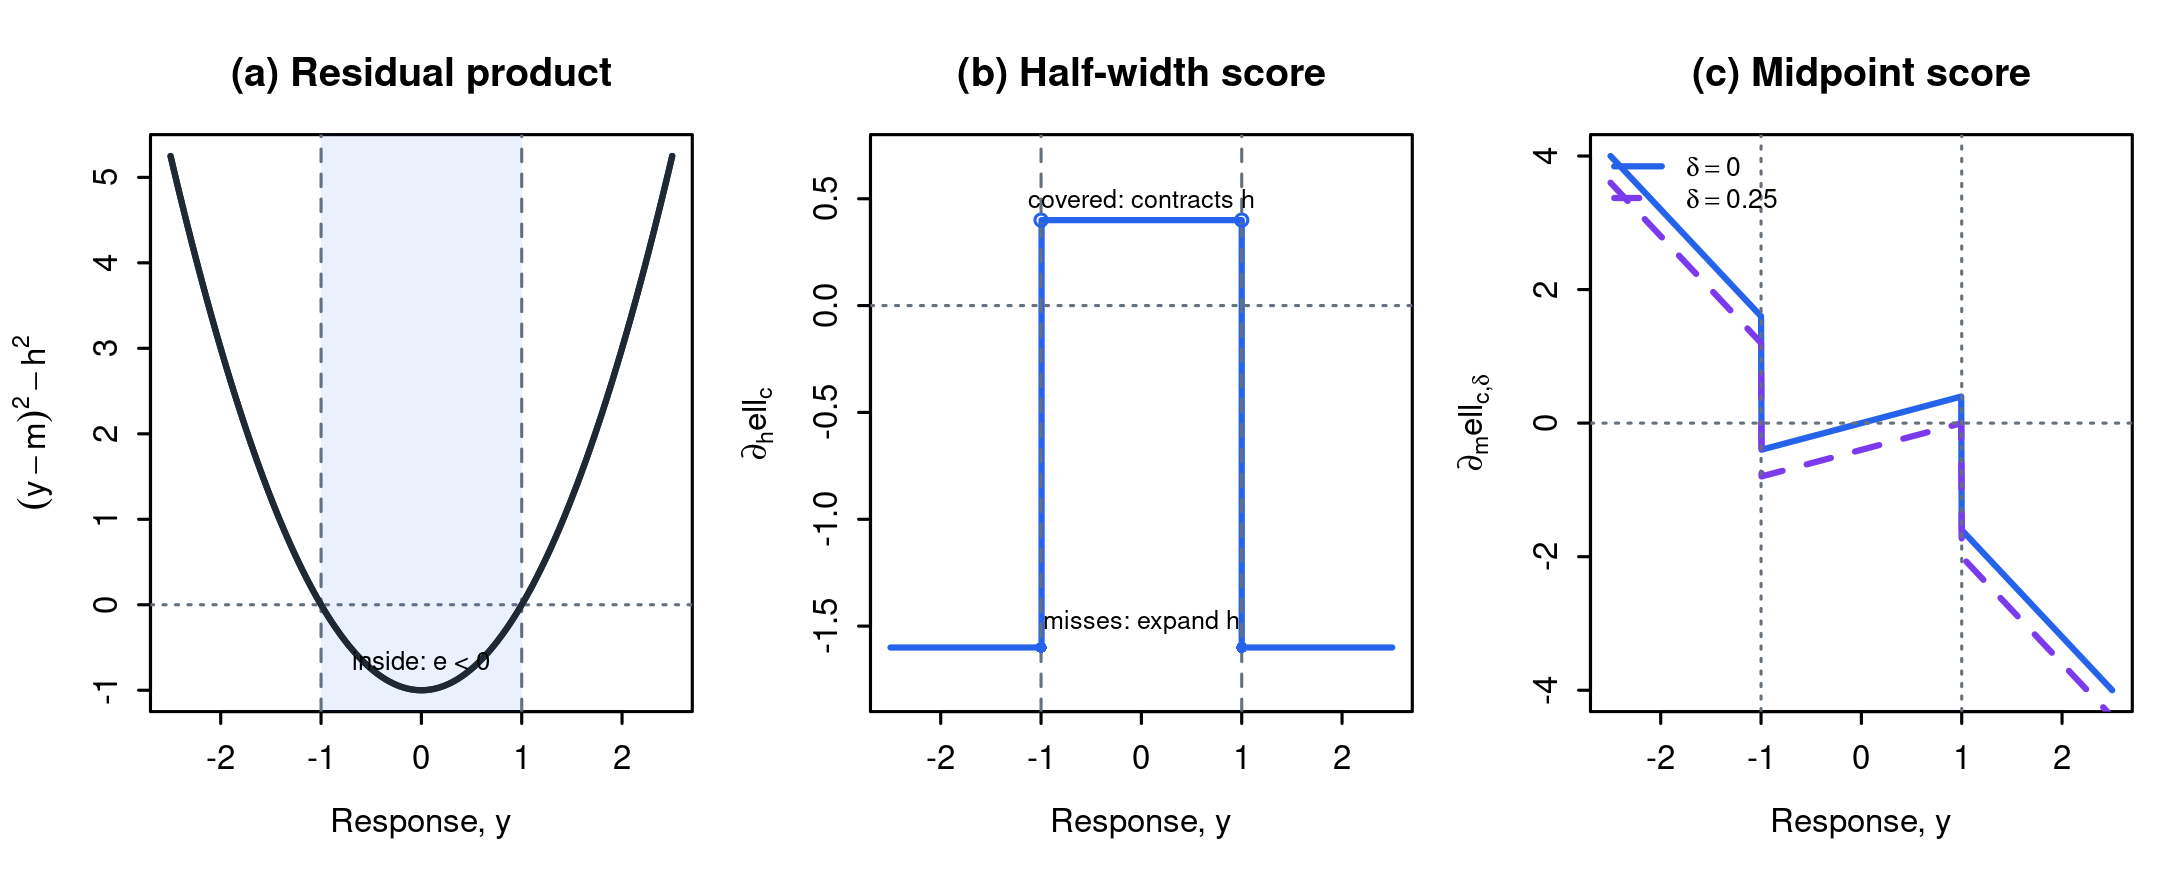
\includegraphics[width=\textwidth]{figures/ch05-mti/generated/figS02_loss_geometry.png}
\caption{\textbf{MPI loss geometry and the fixed midpoint tilt.}
For \(c=0.80\), \(m=0\), and \(h=1\), the residual product is negative exactly
inside the interval. The half-width score contracts \(h\) for covered
observations and expands it for misses. A fixed \(\delta\) adds a constant
shift to the midpoint score but leaves the half-width score unchanged. These
plots use the strict convention \(\ind(e<0)\): filled endpoint marks show the
score at \(y=\pm1\), while open marks show the one-sided inside limits. These
are deterministic pointwise score calculations, not fitted results.}
\label{rqr2026:fig:supp-loss-geometry}
\end{figure}

\subsection{Width-Regularized Interval Loss}
\label{rqr2026:sec:supp-rqr-w}

The width-regularized variant in \citet{rqr-PouplinEtAl2024RQR} has a different
population score system from the MPI loss. For comparison, they use the RQR-W
population objective
\[
\E\left[\rho_q\{(Y-a)(Y-b)\}\right]
+\frac{\lambda_W}{2}(b-a)^2,
\qquad \lambda_W\ge0.
\]
In the present terminology, RQR-W is a width-regularized modification of the
MPI loss, not the MPI loss itself.
At a nondegenerate interior stationary point, subtracting the two endpoint
score equations gives
\[
\Pr(a<Y<b)=q-2\lambda_W.
\]
Thus \(q=c+2\lambda_W\) restores content \(c\), subject to
\(0\le\lambda_W<(1-c)/2\). The midpoint equation then gives
\[
\E(Y\mid a<Y<b)
=\mu+\frac{2\lambda_W}{c}(\mu-m),
\qquad m=\frac{a+b}{2}.
\]
Except in special symmetric cases, RQR-W therefore changes the
mean-preserving placement equation. It is a coverage-corrected compromise
between MPI risk and squared width, not a tie-breaker among
unidentified MPI minimizers.

More generally, if a differentiable width penalty \(P(w)\), \(w=b-a\), is
added to a check loss at level \(q\), the coverage equation is
\[
\Pr(a<Y<b)=q-\frac{2P'(w)}{w}.
\]
A correction independent of the distribution and realized width is possible
only when \(P'(w)/w\) is constant, which yields a quadratic penalty up to an
additive constant. This explains both the form of RQR-W and why its path does
not generally coincide with the shortest-contiguous path.

\subsection{Fixed-Target MTI Computation}
\label{rqr2026:sec:supp-mti-ecm}

The validation study computes endpoint estimates by minimizing a penalized
MTI criterion for each fixed content and tilt. Section~\ref{rqr2026:sec:supp-profiled-intercept}
gives the scalar convex-profile representation used in that calculation.
We first record an alternative expectation/conditional maximization (ECM)
derivation, which explains the augmentation but is not used to produce the
reported candidate endpoints. The complete interval-selection rule is
assessed on independent simulation samples.

For \(e_i=(y_i-\eta_{1i})(y_i-\eta_{2i})\), the fixed-target MTI loss is
\[
L_{n,q,\delta}
=\sum_{i=1}^n\left[
\rho_q(e_i)-q\delta(\eta_{1i}+\eta_{2i}-2y_i)
\right],
\qquad
\rho_q(r)=r\{q-\ind(r<0)\}.
\]
With fixed learning rate \(\omega_{\mathrm R}\), the generalized-posterior
kernel is proportional to
\[
\exp\{-\omega_{\mathrm R}L_{n,q,\delta}(\theta)\}\pi_0(\theta).
\]
The validation calculations are intercept-only, so \(\theta=(a,b)\) before the
two roots are sorted into lower and upper endpoints.

\subsubsection{An Alternative ECM Calculation}

The pseudo-asymmetric-Laplace representation gives a convenient quadratic
conditional calculation. Define
\[
\sigma_{\mathrm R}=\omega_{\mathrm R}^{-1},\qquad
\xi_q=\frac{1-2q}{q(1-q)},\qquad
\phi_q=\frac{2}{q(1-q)}.
\]
Then
\begin{align}
&\frac{q(1-q)}{\sigma_{\mathrm R}}
\exp\{-\rho_q(e_i)/\sigma_{\mathrm R}\}\notag\\
&\quad=\int_0^\infty
\Normal\!\left(e_i\mid\xi_qv_i,\phi_q\sigma_{\mathrm R}v_i\right)
\Exp\!\left(v_i\mid\mathrm{rate}=1/\sigma_{\mathrm R}\right)\,dv_i.
\label{rqr2026:eq:supp-pseudo-al-mixture}
\end{align}
The latent scale is computational; it augments a loss factor rather than a
sampling distribution for \(Y_i\).

Under the \(\GIG(\nu,A,B)\) convention proportional to
\(v^{\nu-1}\exp\{-(Av+B/v)/2\}\), the conditional scale law has
\[
v_i\mid\cdot\sim
\GIG\left\{
\frac12,\
\frac{1}{2\sigma_{\mathrm R}q(1-q)},\
\frac{q(1-q)e_i^2}{2\sigma_{\mathrm R}}
\right\}.
\]
For \(e_i\ne0\),
\[
\tau_i=E(v_i^{-1}\mid\cdot)=\frac{1}{q(1-q)|e_i|}.
\]
The numerical ECM calculation uses a small response-product scale floor when
\(e_i\) is near zero and objective backtracking after each accepted cycle.
An ECM implementation can initialize each candidate from empirical
shortest-window endpoints shifted by its tilt. Multiple initializations can
be compared through the same penalized objective.

\begin{algorithmblock}{Alternative fixed-target ECM calculation}
\begin{enumerate}[leftmargin=2.2em,itemsep=0.3em,parsep=0pt]
\item Fix \(q\), \(\delta\), \(\omega_{\mathrm R}\), the ridge prior precision,
and deterministic starting roots.
\item At the current roots, compute product residuals \(e_i\) and inverse-scale
moments \(\tau_i\), using the prespecified numerical floor only when needed.
\item Holding one root fixed, solve the Gaussian conditional maximization for
the other root. Repeat with the roles exchanged.
\item Accept a full cycle when the exact penalized objective does not increase
beyond the prespecified numerical allowance, using backtracking if necessary.
\item Return the final endpoint estimates and sort the two raw roots to report the
candidate interval. If multiple starts are requested, select the fit with the
smallest exact penalized objective.
\end{enumerate}
\end{algorithmblock}

The fitted content \(q\) and tilt \(\delta\) index fixed-target generalized
posteriors. The procedure profiles over their grid on each training sample.
Grid settings and the DP probability threshold are calibrated separately and
then applied unchanged to independent validation replications.

\subsubsection{The Penalized Intercept Criterion}
\label{rqr2026:sec:supp-profiled-intercept}

The reported estimates use the following profile representation. Let the two
roots have independent zero-mean Gaussian priors with
common precision \(\lambda>0\), and fix \(q\), \(\delta\), and
\(\omega_{\mathrm R}>0\). Their negative log generalized-posterior criterion,
up to a constant, is
\[
J(a,b)=\omega_{\mathrm R}\sum_i
\left[\rho_q\{(y_i-a)(y_i-b)\}-q\delta(a+b-2y_i)\right]
+\frac{\lambda}{2}(a^2+b^2).
\]
Write \(m=(a+b)/2\), \(t=(b-a)^2/4\), and
\(s=nq-\lambda/\omega_{\mathrm R}\). The variable \(t\) is a squared
half-width used to minimize this same criterion; no transformed-density mode
is introduced.

\begin{proposition}[Convex midpoint profile]
\label{rqr2026:prop:supp-convex-intercept-profile}
Suppose \(0<s<n\), and put
\(W_s=\{w\in[0,1]^n:\sum_iw_i=s\}\). For a fixed midpoint, a minimizing
\(t\ge0\) is an empirical \(s/n\) quantile of the squared distances
\((y_i-m)^2\). The profiled criterion has the representation
\begin{align*}
\min_{t\ge0}J(m,t)
={}&2\lambda m^2+\max_{w\in W_s}\{A(w)+B(w)m\},\\
A(w)={}&\omega_{\mathrm R}
\left[q\sum_i y_i^2-\sum_iw_i y_i^2+2q\delta\sum_i y_i\right],\\
B(w)={}&2\omega_{\mathrm R}
\left[\sum_iw_i y_i-q\sum_i y_i-nq\delta\right].
\end{align*}
It is strongly convex in \(m\), so its minimizing midpoint is unique.
The minimizing squared half-width can be nonunique at an empirical quantile.
\end{proposition}

\begin{proof}
For \(z_i=(y_i-m)^2\), write
\(\rho_q(z_i-t)=qz_i-qt+(t-z_i)_+\). Minimization in \(t\) gives
\[
\min_{t\ge0}\left\{\sum_i(t-z_i)_+-st\right\}
=-\min_{w\in W_s}\sum_iw_i z_i.
\]
To verify the identity, order the \(z_i\), assign weight one to the smallest
\(\lfloor s\rfloor\) values, and assign the remaining mass at the next value.
The one-sided derivatives in \(t\) bracket zero at the corresponding quantile.
Expansion of the squared distances gives the displayed profile because
\(\omega_{\mathrm R}(nq-s)=\lambda\). A maximum of affine functions is
convex; adding \(2\lambda m^2\) gives strong convexity. If \(s\le0\),
zero is a minimizing squared half-width and the midpoint follows from a
scalar quadratic.
\end{proof}

At a distinct-root joint subgradient-stationary point, the penalized equations
give fractional allocations satisfying
\[
\sum_iw_i=nq-\lambda/\omega_{\mathrm R},\qquad
\sum_iw_i y_i=nq(\overline y+\delta)
-\frac{\lambda}{\omega_{\mathrm R}}(a+b).
\]
These equations explain the prior contributions to empirical balance.
They also supply a global optimality check for this intercept criterion:
\(\rho_q(e_i)\ge(q-w_i)e_i\) is exact at a compatible stationary pair
\((a_0,b_0)\), and substitution gives
\[
J(a,b)\ge J(a_0,b_0)+\frac{\lambda}{2}
\{(a+b)-(a_0+b_0)\}^2.
\]
This argument requires distinct roots and a joint compatible subgradient
selection. At collapsed roots, the squared-radius boundary condition must
also be checked. Unequal prior precisions and regression require separate
arguments.

\paragraph{Profile calculation and numerical checks.}
For each fixed \((q,\delta)\), the numerical calculation minimizes the scalar
midpoint profile and chooses the lower minimizing squared radius at a tie.
The endpoints are \(m-\sqrt t,m+\sqrt t\). A lower objective bound from the
convex profile supplies a relative objective-gap check, with tolerance
\(10^{-8}\). Every candidate must pass before interval selection. The
calculation uses \(\omega_{\mathrm R}=1\), \(\lambda=10^{-4}\), and zero
prior means throughout the reported simulation and application.

The content grid is refined using \(s=nq-\lambda/\omega_{\mathrm R}\).
Within its initial range, each interval \((r-1,r)\) of positive effective
observation mass receives an interior content if none was already present.
Original contents are retained, and duplicate contents are removed. At each
content, the tilt candidates are zero, the balanced fractional shortest-window
tilt, and seven equally spaced positions from the minimum to the maximum
empirical admissible tilt. These are fixed search rules, rather than choices
made using validation outcomes. The reported shortest-candidate property
applies to this finite search.

\subsection{Direct DP Content Check}
\label{rqr2026:sec:supp-direct-dp-check}

The MTI comparator uses a model-based content-probability check during calibration.
For a fixed closed interval \(I=[l,u]\), let \(N_n(I)=\sum_{i=1}^n\ind(Y_i\in I)\).
Under the direct Dirichlet-process model
\[
F\sim\mathrm{DP}(a,H),\qquad
Y_i\mid F\stackrel{\mathrm{iid}}{\sim}F,
\]
with fixed \(a>0\) and fixed base distribution \(H\), conjugacy gives an exact
posterior law for the interval content. The reported calculations use
\(a=1\) and \(H=\Normal(0,4^2)\), fixed on the response scale used for fitting.

\begin{proposition}[Direct DP fixed-interval content law]
\label{rqr2026:prop:supp-dp-content-law}
For fixed \(I=[l,u]\),
\[
F(I)\mid D_n\sim
\mathrm{Beta}\{aH(I)+N_n(I),a(1-H(I))+n-N_n(I)\}.
\]
Consequently \(p_n(I;c)=\Pr\{F(I)\ge c\mid D_n\}\) is available from a Beta
survival probability.
\end{proposition}

\begin{proof}
Dirichlet-process conjugacy gives
\[
F\mid D_n\sim \mathrm{DP}(a+n,H_n),\qquad
H_n=\frac{aH+\sum_{i=1}^n\delta_{Y_i}}{a+n}.
\]
For the partition \((I,I^c)\), the finite-dimensional distribution of a
Dirichlet process is Dirichlet with parameters
\((a+n)H_n(I)=aH(I)+N_n(I)\) and
\((a+n)H_n(I^c)=a\{1-H(I)\}+n-N_n(I)\). The first coordinate is the stated
Beta distribution.
\end{proof}

The direct DP check determines eligible MTI candidates for each training
sample. Its threshold is chosen in a separate calibration run and fixed before
independent validation. The Beta identity is a posterior probability statement
under the DP response-distribution model. The repeated-sampling behavior of
the selected interval is assessed empirically.

\subsection{Tolerance-Validation Protocol and Feasibility}
\label{rqr2026:sec:supp-tolerance-validation-protocol}

The primary tolerance validation is restricted to iid continuous univariate
samples. The comparison includes the calibrated MTI rule, Young--Mathew
interpolation, and Wilks full-range intervals. MTI
profiles fixed-target endpoint fits over fitted content and retained-mean tilt,
then applies a direct Dirichlet-process fixed-interval content probability
threshold. Its cutoff is determined by simultaneous simulation-calibration
bounds. The scan reference below initializes the content grid. Young--Mathew and Wilks are classical order-statistic
comparators. Regression and dynamic tolerance calibration require additional
results because the fitted intervals vary with covariates or time.

The simulation design fixes tolerance confidence \(1-\alpha=0.95\) and uses
explicit feasible design cells:
\[
  \begin{aligned}
  (n,c)\in\{&
  (50,0.90),(100,0.90),(100,0.95),\\
  &(500,0.90),(500,0.95),(500,0.99),\\
  &(1000,0.90),(1000,0.95),(1000,0.99)\}.
  \end{aligned}
\]
The distributional panel contains two symmetric reference distributions and six
asymmetric simulation distributions. The symmetric reference distributions are
Gaussian and Student \(t_3\). The asymmetric simulation distributions are
exponential, asymmetric Laplace with \(\tau=0.10\), two-piece Normal with scale
ratio \(1{:}12\), Beta\((1,8)\), Gamma\((0.5,1)\), and log-normal with
log-scale standard deviation \(1.25\). All laws are centered and scaled before
sampling. Within each cell, all three methods use common random samples,
independent of threshold development and calibration assessment. The
reproducibility materials include the code version, simulation settings,
package versions, random seeds, calibration files, and numerical summaries.
The article comparison uses the three methods from this paired independent
validation. The reported rows contribute 216,000
replication-level method evaluations over the 72 distribution-level cells used in the main
comparison. A frozen earlier MTI specification is evaluated on the same samples
as a numerical comparison in the reproducibility materials. All simulations completed, and all three reported methods produced
an interval in every replication. The manuscript tables and figures are
computed directly from these replication-level simulation outputs and the
corresponding scan-calibration outputs. The scenario-range table in the main
article is summarized across distributions within each \((n,c)\) cell, while
the integrated tables retain the distribution-level content-attainment and width
summaries.
Table~\ref{rqr2026:tab:supp-primary-dgp-delivery} gives the distribution-level
content-attainment percentages before aggregation, and
Table~\ref{rqr2026:tab:supp-primary-dgp-width-ranges} reports the corresponding
distribution-level 2.5\%--97.5\% ranges of interval lengths. The
replication-level data file records indicators of interval production,
infeasibility indicators, and raw width summaries for each
distribution-level cell as reproducibility information.

\paragraph{Threshold development and assessment.}
For each setting, 32 development samples per distribution determine a finite
cutoff menu from 25 empirical quantiles of candidate posterior probabilities
and the requested tolerance confidence. A separate 24,000 samples per
distribution assess every cutoff. We select the smallest cutoff that returns
every interval and whose one-sided exact binomial lower bound for attainment
is at least \(0.95\) in every distribution.

Seven of nine settings pass the initial assessment. A fixed follow-up uses
fresh development and assessment samples for \(n=50,c=0.90\) and
\(n=100,c=0.95\).
For these two settings, the development menu also includes the smallest,
across development samples, of the largest candidate content probability.
Each gap between adjacent probability knots is subdivided into four intervals
on the logit scale. This produces 105 assessed cutoffs in each setting.
The follow-up retains the original seven cutoffs exactly.

The total Monte Carlo error probability is \(0.05\). Half is allocated across
all original nine settings, eight distributions, and 26 cutoffs, giving
per-comparison error \(0.025/(9\cdot8\cdot26)\). The retained seven
cutoffs still pass these tighter bounds. The other half is allocated to the
two fresh settings, eight distributions, and the \(M\) cutoffs determined by
independent development, giving \(0.025/(2\cdot8\cdot M)\). The union bound
controls the combined calibration error. This calculation concerns the fixed
simulation panel. Table~\ref{rqr2026:tab:supp-mti-profile-policy} records the resulting
cutoffs, smallest calibration lower bounds, and independent validation ranges.

\paragraph{Independent uncertainty assessment.}
The cutoff is fixed before the 1000 validation samples per case are generated.
Pointwise exact 95\% binomial intervals accompany each attainment estimate.
For MTI, simultaneous two-sided intervals across 72 cases allocate
\(0.05/(2\cdot72)\) to each tail. Their lower bounds exceed \(0.95\) in
38 cases; 34 include \(0.95\), and none has an upper bound below it.
The smallest point estimate, \(951/1000\), occurs for Student \(t_3\) at
\(n=500,c=0.99\), with pointwise interval approximately
\([0.9357,0.9635]\). Inconclusive validation intervals reflect Monte Carlo
precision and are reported alongside the larger calibration assessment.

\begingroup
\TableStyle
\begingroup
\footnotesize
\setlength{\tabcolsep}{3pt}
\begin{longtable}{@{}rrlrr@{}}
\caption{\textbf{Content attainment by distribution.} Each estimate uses 1000 paired samples. Brackets give pointwise exact 95\% Monte Carlo confidence intervals.}\label{rqr2026:tab:supp-primary-dgp-delivery}\\
\toprule
\(n\) & \(c\) & Method & Attainment (\%) & 95\% confidence interval\\
\midrule
\endfirsthead
\toprule
\(n\) & \(c\) & Method & Attainment (\%) & 95\% confidence interval\\
\midrule
\endhead
\multicolumn{5}{@{}l}{\textit{Asymmetric Laplace (tau=0.10)}}\\
50 & 0.90 & MTI & 96.1 & [94.7, 97.2] \\
 &  & Young--Mathew & 95.6 & [94.1, 96.8] \\
 &  & Wilks & 96.1 & [94.7, 97.2] \\
\addlinespace[0.2em]
100 & 0.90 & MTI & 96.7 & [95.4, 97.7] \\
 &  & Young--Mathew & 97.2 & [96.0, 98.1] \\
 &  & Wilks & 100.0 & [99.6, 100.0] \\
\addlinespace[0.2em]
100 & 0.95 & MTI & 96.1 & [94.7, 97.2] \\
 &  & Young--Mathew & 95.6 & [94.1, 96.8] \\
 &  & Wilks & 96.1 & [94.7, 97.2] \\
\addlinespace[0.2em]
500 & 0.90 & MTI & 97.9 & [96.8, 98.7] \\
 &  & Young--Mathew & 95.5 & [94.0, 96.7] \\
 &  & Wilks & 100.0 & [99.6, 100.0] \\
\addlinespace[0.2em]
500 & 0.95 & MTI & 97.5 & [96.3, 98.4] \\
 &  & Young--Mathew & 94.6 & [93.0, 95.9] \\
 &  & Wilks & 100.0 & [99.6, 100.0] \\
\addlinespace[0.2em]
500 & 0.99 & MTI & 96.9 & [95.6, 97.9] \\
 &  & Young--Mathew & 96.5 & [95.2, 97.6] \\
 &  & Wilks & 96.9 & [95.6, 97.9] \\
\addlinespace[0.2em]
1000 & 0.90 & MTI & 96.9 & [95.6, 97.9] \\
 &  & Young--Mathew & 95.1 & [93.6, 96.4] \\
 &  & Wilks & 100.0 & [99.6, 100.0] \\
\addlinespace[0.2em]
1000 & 0.95 & MTI & 98.7 & [97.8, 99.3] \\
 &  & Young--Mathew & 96.2 & [94.8, 97.3] \\
 &  & Wilks & 100.0 & [99.6, 100.0] \\
\addlinespace[0.2em]
1000 & 0.99 & MTI & 98.1 & [97.0, 98.9] \\
 &  & Young--Mathew & 95.9 & [94.5, 97.0] \\
 &  & Wilks & 99.9 & [99.4, 100.0] \\
\addlinespace[0.2em]
\multicolumn{5}{@{}l}{\textit{Beta(1,8)}}\\
50 & 0.90 & MTI & 96.4 & [95.1, 97.5] \\
 &  & Young--Mathew & 95.4 & [93.9, 96.6] \\
 &  & Wilks & 96.4 & [95.1, 97.5] \\
\addlinespace[0.2em]
100 & 0.90 & MTI & 97.5 & [96.3, 98.4] \\
 &  & Young--Mathew & 96.4 & [95.1, 97.5] \\
 &  & Wilks & 100.0 & [99.6, 100.0] \\
\addlinespace[0.2em]
100 & 0.95 & MTI & 95.7 & [94.3, 96.9] \\
 &  & Young--Mathew & 95.1 & [93.6, 96.4] \\
 &  & Wilks & 95.7 & [94.3, 96.9] \\
\addlinespace[0.2em]
500 & 0.90 & MTI & 98.4 & [97.4, 99.1] \\
 &  & Young--Mathew & 95.7 & [94.3, 96.9] \\
 &  & Wilks & 100.0 & [99.6, 100.0] \\
\addlinespace[0.2em]
500 & 0.95 & MTI & 98.8 & [97.9, 99.4] \\
 &  & Young--Mathew & 94.8 & [93.2, 96.1] \\
 &  & Wilks & 100.0 & [99.6, 100.0] \\
\addlinespace[0.2em]
500 & 0.99 & MTI & 96.2 & [94.8, 97.3] \\
 &  & Young--Mathew & 95.7 & [94.3, 96.9] \\
 &  & Wilks & 96.2 & [94.8, 97.3] \\
\addlinespace[0.2em]
1000 & 0.90 & MTI & 99.0 & [98.2, 99.5] \\
 &  & Young--Mathew & 95.3 & [93.8, 96.5] \\
 &  & Wilks & 100.0 & [99.6, 100.0] \\
\addlinespace[0.2em]
1000 & 0.95 & MTI & 99.1 & [98.3, 99.6] \\
 &  & Young--Mathew & 94.8 & [93.2, 96.1] \\
 &  & Wilks & 100.0 & [99.6, 100.0] \\
\addlinespace[0.2em]
1000 & 0.99 & MTI & 99.0 & [98.2, 99.5] \\
 &  & Young--Mathew & 95.0 & [93.5, 96.3] \\
 &  & Wilks & 99.9 & [99.4, 100.0] \\
\addlinespace[0.2em]
\multicolumn{5}{@{}l}{\textit{Exponential}}\\
50 & 0.90 & MTI & 98.0 & [96.9, 98.8] \\
 &  & Young--Mathew & 96.9 & [95.6, 97.9] \\
 &  & Wilks & 98.0 & [96.9, 98.8] \\
\addlinespace[0.2em]
100 & 0.90 & MTI & 97.3 & [96.1, 98.2] \\
 &  & Young--Mathew & 95.1 & [93.6, 96.4] \\
 &  & Wilks & 100.0 & [99.6, 100.0] \\
\addlinespace[0.2em]
100 & 0.95 & MTI & 96.5 & [95.2, 97.6] \\
 &  & Young--Mathew & 95.7 & [94.3, 96.9] \\
 &  & Wilks & 96.5 & [95.2, 97.6] \\
\addlinespace[0.2em]
500 & 0.90 & MTI & 98.2 & [97.2, 98.9] \\
 &  & Young--Mathew & 96.1 & [94.7, 97.2] \\
 &  & Wilks & 100.0 & [99.6, 100.0] \\
\addlinespace[0.2em]
500 & 0.95 & MTI & 98.0 & [96.9, 98.8] \\
 &  & Young--Mathew & 95.8 & [94.4, 97.0] \\
 &  & Wilks & 100.0 & [99.6, 100.0] \\
\addlinespace[0.2em]
500 & 0.99 & MTI & 97.3 & [96.1, 98.2] \\
 &  & Young--Mathew & 97.2 & [96.0, 98.1] \\
 &  & Wilks & 97.3 & [96.1, 98.2] \\
\addlinespace[0.2em]
1000 & 0.90 & MTI & 98.5 & [97.5, 99.2] \\
 &  & Young--Mathew & 94.9 & [93.3, 96.2] \\
 &  & Wilks & 100.0 & [99.6, 100.0] \\
\addlinespace[0.2em]
1000 & 0.95 & MTI & 99.0 & [98.2, 99.5] \\
 &  & Young--Mathew & 95.7 & [94.3, 96.9] \\
 &  & Wilks & 100.0 & [99.6, 100.0] \\
\addlinespace[0.2em]
1000 & 0.99 & MTI & 98.6 & [97.7, 99.2] \\
 &  & Young--Mathew & 95.0 & [93.5, 96.3] \\
 &  & Wilks & 100.0 & [99.6, 100.0] \\
\addlinespace[0.2em]
\multicolumn{5}{@{}l}{\textit{Gamma(0.5,1)}}\\
50 & 0.90 & MTI & 96.5 & [95.2, 97.6] \\
 &  & Young--Mathew & 96.0 & [94.6, 97.1] \\
 &  & Wilks & 96.5 & [95.2, 97.6] \\
\addlinespace[0.2em]
100 & 0.90 & MTI & 98.3 & [97.3, 99.0] \\
 &  & Young--Mathew & 96.2 & [94.8, 97.3] \\
 &  & Wilks & 100.0 & [99.6, 100.0] \\
\addlinespace[0.2em]
100 & 0.95 & MTI & 97.3 & [96.1, 98.2] \\
 &  & Young--Mathew & 96.9 & [95.6, 97.9] \\
 &  & Wilks & 97.3 & [96.1, 98.2] \\
\addlinespace[0.2em]
500 & 0.90 & MTI & 98.8 & [97.9, 99.4] \\
 &  & Young--Mathew & 94.5 & [92.9, 95.8] \\
 &  & Wilks & 100.0 & [99.6, 100.0] \\
\addlinespace[0.2em]
500 & 0.95 & MTI & 98.9 & [98.0, 99.4] \\
 &  & Young--Mathew & 95.7 & [94.3, 96.9] \\
 &  & Wilks & 100.0 & [99.6, 100.0] \\
\addlinespace[0.2em]
500 & 0.99 & MTI & 97.1 & [95.9, 98.0] \\
 &  & Young--Mathew & 96.9 & [95.6, 97.9] \\
 &  & Wilks & 97.1 & [95.9, 98.0] \\
\addlinespace[0.2em]
1000 & 0.90 & MTI & 99.3 & [98.6, 99.7] \\
 &  & Young--Mathew & 95.4 & [93.9, 96.6] \\
 &  & Wilks & 100.0 & [99.6, 100.0] \\
\addlinespace[0.2em]
1000 & 0.95 & MTI & 98.7 & [97.8, 99.3] \\
 &  & Young--Mathew & 94.7 & [93.1, 96.0] \\
 &  & Wilks & 100.0 & [99.6, 100.0] \\
\addlinespace[0.2em]
1000 & 0.99 & MTI & 98.7 & [97.8, 99.3] \\
 &  & Young--Mathew & 94.5 & [92.9, 95.8] \\
 &  & Wilks & 99.9 & [99.4, 100.0] \\
\addlinespace[0.2em]
\multicolumn{5}{@{}l}{\textit{Log-normal (log sd 1.25)}}\\
50 & 0.90 & MTI & 96.5 & [95.2, 97.6] \\
 &  & Young--Mathew & 95.9 & [94.5, 97.0] \\
 &  & Wilks & 96.5 & [95.2, 97.6] \\
\addlinespace[0.2em]
100 & 0.90 & MTI & 98.0 & [96.9, 98.8] \\
 &  & Young--Mathew & 96.8 & [95.5, 97.8] \\
 &  & Wilks & 100.0 & [99.6, 100.0] \\
\addlinespace[0.2em]
100 & 0.95 & MTI & 96.7 & [95.4, 97.7] \\
 &  & Young--Mathew & 96.3 & [94.9, 97.4] \\
 &  & Wilks & 96.7 & [95.4, 97.7] \\
\addlinespace[0.2em]
500 & 0.90 & MTI & 99.1 & [98.3, 99.6] \\
 &  & Young--Mathew & 95.9 & [94.5, 97.0] \\
 &  & Wilks & 100.0 & [99.6, 100.0] \\
\addlinespace[0.2em]
500 & 0.95 & MTI & 98.6 & [97.7, 99.2] \\
 &  & Young--Mathew & 95.4 & [93.9, 96.6] \\
 &  & Wilks & 100.0 & [99.6, 100.0] \\
\addlinespace[0.2em]
500 & 0.99 & MTI & 95.8 & [94.4, 97.0] \\
 &  & Young--Mathew & 95.2 & [93.7, 96.4] \\
 &  & Wilks & 95.8 & [94.4, 97.0] \\
\addlinespace[0.2em]
1000 & 0.90 & MTI & 99.2 & [98.4, 99.7] \\
 &  & Young--Mathew & 95.1 & [93.6, 96.4] \\
 &  & Wilks & 100.0 & [99.6, 100.0] \\
\addlinespace[0.2em]
1000 & 0.95 & MTI & 98.6 & [97.7, 99.2] \\
 &  & Young--Mathew & 95.1 & [93.6, 96.4] \\
 &  & Wilks & 100.0 & [99.6, 100.0] \\
\addlinespace[0.2em]
1000 & 0.99 & MTI & 99.3 & [98.6, 99.7] \\
 &  & Young--Mathew & 94.7 & [93.1, 96.0] \\
 &  & Wilks & 100.0 & [99.6, 100.0] \\
\addlinespace[0.2em]
\multicolumn{5}{@{}l}{\textit{Gaussian}}\\
50 & 0.90 & MTI & 96.6 & [95.3, 97.6] \\
 &  & Young--Mathew & 96.0 & [94.6, 97.1] \\
 &  & Wilks & 96.6 & [95.3, 97.6] \\
\addlinespace[0.2em]
100 & 0.90 & MTI & 96.4 & [95.1, 97.5] \\
 &  & Young--Mathew & 97.9 & [96.8, 98.7] \\
 &  & Wilks & 100.0 & [99.6, 100.0] \\
\addlinespace[0.2em]
100 & 0.95 & MTI & 95.6 & [94.1, 96.8] \\
 &  & Young--Mathew & 95.4 & [93.9, 96.6] \\
 &  & Wilks & 95.6 & [94.1, 96.8] \\
\addlinespace[0.2em]
500 & 0.90 & MTI & 96.0 & [94.6, 97.1] \\
 &  & Young--Mathew & 96.3 & [94.9, 97.4] \\
 &  & Wilks & 100.0 & [99.6, 100.0] \\
\addlinespace[0.2em]
500 & 0.95 & MTI & 98.1 & [97.0, 98.9] \\
 &  & Young--Mathew & 98.3 & [97.3, 99.0] \\
 &  & Wilks & 100.0 & [99.6, 100.0] \\
\addlinespace[0.2em]
500 & 0.99 & MTI & 96.3 & [94.9, 97.4] \\
 &  & Young--Mathew & 96.0 & [94.6, 97.1] \\
 &  & Wilks & 96.3 & [94.9, 97.4] \\
\addlinespace[0.2em]
1000 & 0.90 & MTI & 96.8 & [95.5, 97.8] \\
 &  & Young--Mathew & 95.6 & [94.1, 96.8] \\
 &  & Wilks & 100.0 & [99.6, 100.0] \\
\addlinespace[0.2em]
1000 & 0.95 & MTI & 95.9 & [94.5, 97.0] \\
 &  & Young--Mathew & 96.4 & [95.1, 97.5] \\
 &  & Wilks & 100.0 & [99.6, 100.0] \\
\addlinespace[0.2em]
1000 & 0.99 & MTI & 97.5 & [96.3, 98.4] \\
 &  & Young--Mathew & 96.8 & [95.5, 97.8] \\
 &  & Wilks & 100.0 & [99.6, 100.0] \\
\addlinespace[0.2em]
\multicolumn{5}{@{}l}{\textit{Student t(3)}}\\
50 & 0.90 & MTI & 97.5 & [96.3, 98.4] \\
 &  & Young--Mathew & 96.9 & [95.6, 97.9] \\
 &  & Wilks & 97.5 & [96.3, 98.4] \\
\addlinespace[0.2em]
100 & 0.90 & MTI & 96.0 & [94.6, 97.1] \\
 &  & Young--Mathew & 97.3 & [96.1, 98.2] \\
 &  & Wilks & 100.0 & [99.6, 100.0] \\
\addlinespace[0.2em]
100 & 0.95 & MTI & 96.4 & [95.1, 97.5] \\
 &  & Young--Mathew & 96.1 & [94.7, 97.2] \\
 &  & Wilks & 96.4 & [95.1, 97.5] \\
\addlinespace[0.2em]
500 & 0.90 & MTI & 96.4 & [95.1, 97.5] \\
 &  & Young--Mathew & 96.6 & [95.3, 97.6] \\
 &  & Wilks & 100.0 & [99.6, 100.0] \\
\addlinespace[0.2em]
500 & 0.95 & MTI & 98.5 & [97.5, 99.2] \\
 &  & Young--Mathew & 97.2 & [96.0, 98.1] \\
 &  & Wilks & 100.0 & [99.6, 100.0] \\
\addlinespace[0.2em]
500 & 0.99 & MTI & 95.1 & [93.6, 96.4] \\
 &  & Young--Mathew & 95.0 & [93.5, 96.3] \\
 &  & Wilks & 95.1 & [93.6, 96.4] \\
\addlinespace[0.2em]
1000 & 0.90 & MTI & 95.7 & [94.3, 96.9] \\
 &  & Young--Mathew & 94.1 & [92.5, 95.5] \\
 &  & Wilks & 100.0 & [99.6, 100.0] \\
\addlinespace[0.2em]
1000 & 0.95 & MTI & 96.9 & [95.6, 97.9] \\
 &  & Young--Mathew & 96.6 & [95.3, 97.6] \\
 &  & Wilks & 100.0 & [99.6, 100.0] \\
\addlinespace[0.2em]
1000 & 0.99 & MTI & 98.5 & [97.5, 99.2] \\
 &  & Young--Mathew & 97.9 & [96.8, 98.7] \\
 &  & Wilks & 99.9 & [99.4, 100.0] \\
\addlinespace[0.2em]
\multicolumn{5}{@{}l}{\textit{Two-piece Normal (1:12)}}\\
50 & 0.90 & MTI & 97.0 & [95.7, 98.0] \\
 &  & Young--Mathew & 96.1 & [94.7, 97.2] \\
 &  & Wilks & 97.0 & [95.7, 98.0] \\
\addlinespace[0.2em]
100 & 0.90 & MTI & 95.5 & [94.0, 96.7] \\
 &  & Young--Mathew & 96.6 & [95.3, 97.6] \\
 &  & Wilks & 100.0 & [99.6, 100.0] \\
\addlinespace[0.2em]
100 & 0.95 & MTI & 97.1 & [95.9, 98.0] \\
 &  & Young--Mathew & 96.9 & [95.6, 97.9] \\
 &  & Wilks & 97.1 & [95.9, 98.0] \\
\addlinespace[0.2em]
500 & 0.90 & MTI & 97.2 & [96.0, 98.1] \\
 &  & Young--Mathew & 95.3 & [93.8, 96.5] \\
 &  & Wilks & 100.0 & [99.6, 100.0] \\
\addlinespace[0.2em]
500 & 0.95 & MTI & 97.1 & [95.9, 98.0] \\
 &  & Young--Mathew & 95.0 & [93.5, 96.3] \\
 &  & Wilks & 100.0 & [99.6, 100.0] \\
\addlinespace[0.2em]
500 & 0.99 & MTI & 95.5 & [94.0, 96.7] \\
 &  & Young--Mathew & 95.1 & [93.6, 96.4] \\
 &  & Wilks & 95.5 & [94.0, 96.7] \\
\addlinespace[0.2em]
1000 & 0.90 & MTI & 96.9 & [95.6, 97.9] \\
 &  & Young--Mathew & 94.2 & [92.6, 95.6] \\
 &  & Wilks & 100.0 & [99.6, 100.0] \\
\addlinespace[0.2em]
1000 & 0.95 & MTI & 98.2 & [97.2, 98.9] \\
 &  & Young--Mathew & 95.3 & [93.8, 96.5] \\
 &  & Wilks & 100.0 & [99.6, 100.0] \\
\addlinespace[0.2em]
1000 & 0.99 & MTI & 98.5 & [97.5, 99.2] \\
 &  & Young--Mathew & 96.4 & [95.1, 97.5] \\
 &  & Wilks & 100.0 & [99.6, 100.0] \\
\addlinespace[0.2em]
\bottomrule
\end{longtable}
\endgroup

\endgroup

\begingroup
\scriptsize
\setlength{\tabcolsep}{3pt}
\begin{longtable}{@{}rrlrr@{}}
\caption{\textbf{Interval widths by distribution and design.} Width ranges are empirical 2.5\%--97.5\% quantiles within each case and method.}\label{rqr2026:tab:supp-primary-dgp-width-ranges}\\
\toprule
\(n\) & \(c\) & Method & Attainment (\%) & Width 95\% range\\
\midrule
\endfirsthead
\toprule
\(n\) & \(c\) & Method & Attainment (\%) & Width 95\% range\\
\midrule
\endhead
\multicolumn{5}{@{}l}{\textit{Gaussian}}\\
50 & 0.90 & MTI & 96.6 & 3.360--5.870 \\
 &  & Young--Mathew & 96.0 & 3.309--5.674 \\
 &  & Wilks & 96.6 & 3.360--5.870 \\
\addlinespace[0.25em]
100 & 0.90 & MTI & 96.4 & 3.283--4.424 \\
 &  & Young--Mathew & 97.9 & 3.396--4.905 \\
 &  & Wilks & 100.0 & 3.961--6.404 \\
\addlinespace[0.25em]
100 & 0.95 & MTI & 95.6 & 3.929--6.244 \\
 &  & Young--Mathew & 95.4 & 3.893--6.041 \\
 &  & Wilks & 95.6 & 3.929--6.244 \\
\addlinespace[0.25em]
500 & 0.90 & MTI & 96.0 & 3.298--3.833 \\
 &  & Young--Mathew & 96.3 & 3.278--3.826 \\
 &  & Wilks & 100.0 & 5.213--7.221 \\
\addlinespace[0.25em]
500 & 0.95 & MTI & 98.1 & 3.972--4.651 \\
 &  & Young--Mathew & 98.3 & 3.949--4.679 \\
 &  & Wilks & 100.0 & 5.200--7.185 \\
\addlinespace[0.25em]
500 & 0.99 & MTI & 96.3 & 5.197--7.229 \\
 &  & Young--Mathew & 96.0 & 5.169--7.116 \\
 &  & Wilks & 96.3 & 5.197--7.229 \\
\addlinespace[0.25em]
1000 & 0.90 & MTI & 96.8 & 3.292--3.665 \\
 &  & Young--Mathew & 95.6 & 3.281--3.654 \\
 &  & Wilks & 100.0 & 5.595--7.611 \\
\addlinespace[0.25em]
1000 & 0.95 & MTI & 95.9 & 3.919--4.407 \\
 &  & Young--Mathew & 96.4 & 3.913--4.415 \\
 &  & Wilks & 100.0 & 5.661--7.570 \\
\addlinespace[0.25em]
1000 & 0.99 & MTI & 97.5 & 5.217--6.452 \\
 &  & Young--Mathew & 96.8 & 5.196--6.399 \\
 &  & Wilks & 100.0 & 5.620--7.584 \\
\addlinespace[0.25em]
\multicolumn{5}{@{}l}{\textit{Student t(3)}}\\
50 & 0.90 & MTI & 97.5 & 2.923--10.067 \\
 &  & Young--Mathew & 96.9 & 2.873--9.893 \\
 &  & Wilks & 97.5 & 2.923--11.022 \\
\addlinespace[0.25em]
100 & 0.90 & MTI & 96.0 & 2.740--4.989 \\
 &  & Young--Mathew & 97.3 & 2.936--6.661 \\
 &  & Wilks & 100.0 & 3.833--14.128 \\
\addlinespace[0.25em]
100 & 0.95 & MTI & 96.4 & 3.839--13.513 \\
 &  & Young--Mathew & 96.1 & 3.761--14.242 \\
 &  & Wilks & 96.4 & 3.839--15.599 \\
\addlinespace[0.25em]
500 & 0.90 & MTI & 96.4 & 2.730--3.544 \\
 &  & Young--Mathew & 96.6 & 2.708--3.541 \\
 &  & Wilks & 100.0 & 6.818--30.103 \\
\addlinespace[0.25em]
500 & 0.95 & MTI & 98.5 & 3.779--5.276 \\
 &  & Young--Mathew & 97.2 & 3.718--5.466 \\
 &  & Wilks & 100.0 & 6.812--30.956 \\
\addlinespace[0.25em]
500 & 0.99 & MTI & 95.1 & 6.765--18.982 \\
 &  & Young--Mathew & 95.0 & 6.694--23.511 \\
 &  & Wilks & 95.1 & 6.765--25.143 \\
\addlinespace[0.25em]
1000 & 0.90 & MTI & 95.7 & 2.704--3.251 \\
 &  & Young--Mathew & 94.1 & 2.683--3.236 \\
 &  & Wilks & 100.0 & 8.945--32.926 \\
\addlinespace[0.25em]
1000 & 0.95 & MTI & 96.9 & 3.689--4.633 \\
 &  & Young--Mathew & 96.6 & 3.675--4.641 \\
 &  & Wilks & 100.0 & 9.055--33.163 \\
\addlinespace[0.25em]
1000 & 0.99 & MTI & 98.5 & 7.301--13.402 \\
 &  & Young--Mathew & 97.9 & 7.246--14.926 \\
 &  & Wilks & 99.9 & 8.938--34.261 \\
\addlinespace[0.25em]
\multicolumn{5}{@{}l}{\textit{Exponential}}\\
50 & 0.90 & MTI & 98.0 & 2.609--7.609 \\
 &  & Young--Mathew & 96.9 & 2.590--6.962 \\
 &  & Wilks & 98.0 & 2.609--7.609 \\
\addlinespace[0.25em]
100 & 0.90 & MTI & 97.3 & 2.414--4.441 \\
 &  & Young--Mathew & 95.1 & 2.852--6.079 \\
 &  & Wilks & 100.0 & 3.297--8.354 \\
\addlinespace[0.25em]
100 & 0.95 & MTI & 96.5 & 3.260--8.146 \\
 &  & Young--Mathew & 95.7 & 3.223--7.672 \\
 &  & Wilks & 96.5 & 3.260--8.146 \\
\addlinespace[0.25em]
500 & 0.90 & MTI & 98.2 & 2.344--3.009 \\
 &  & Young--Mathew & 96.1 & 2.830--3.752 \\
 &  & Wilks & 100.0 & 4.933--9.447 \\
\addlinespace[0.25em]
500 & 0.95 & MTI & 98.0 & 3.090--4.114 \\
 &  & Young--Mathew & 95.8 & 3.537--4.883 \\
 &  & Wilks & 100.0 & 4.880--9.954 \\
\addlinespace[0.25em]
500 & 0.99 & MTI & 97.3 & 5.021--9.801 \\
 &  & Young--Mathew & 97.2 & 4.976--9.388 \\
 &  & Wilks & 97.3 & 5.021--9.801 \\
\addlinespace[0.25em]
1000 & 0.90 & MTI & 98.5 & 2.337--2.763 \\
 &  & Young--Mathew & 94.9 & 2.855--3.453 \\
 &  & Wilks & 100.0 & 5.581--10.284 \\
\addlinespace[0.25em]
1000 & 0.95 & MTI & 99.0 & 3.074--3.709 \\
 &  & Young--Mathew & 95.7 & 3.564--4.400 \\
 &  & Wilks & 100.0 & 5.603--10.517 \\
\addlinespace[0.25em]
1000 & 0.99 & MTI & 98.6 & 4.917--7.377 \\
 &  & Young--Mathew & 95.0 & 5.133--8.330 \\
 &  & Wilks & 100.0 & 5.615--10.540 \\
\addlinespace[0.25em]
\multicolumn{5}{@{}l}{\textit{Asymmetric Laplace (tau=0.10)}}\\
50 & 0.90 & MTI & 96.1 & 2.793--7.789 \\
 &  & Young--Mathew & 95.6 & 2.722--7.100 \\
 &  & Wilks & 96.1 & 2.793--7.789 \\
\addlinespace[0.25em]
100 & 0.90 & MTI & 96.7 & 2.615--4.577 \\
 &  & Young--Mathew & 97.2 & 2.993--6.044 \\
 &  & Wilks & 100.0 & 3.590--8.542 \\
\addlinespace[0.25em]
100 & 0.95 & MTI & 96.1 & 3.554--8.688 \\
 &  & Young--Mathew & 95.6 & 3.522--8.174 \\
 &  & Wilks & 96.1 & 3.554--8.688 \\
\addlinespace[0.25em]
500 & 0.90 & MTI & 97.9 & 2.572--3.272 \\
 &  & Young--Mathew & 95.5 & 2.847--3.745 \\
 &  & Wilks & 100.0 & 5.231--10.159 \\
\addlinespace[0.25em]
500 & 0.95 & MTI & 97.5 & 3.337--4.470 \\
 &  & Young--Mathew & 94.6 & 3.590--4.982 \\
 &  & Wilks & 100.0 & 5.181--10.425 \\
\addlinespace[0.25em]
500 & 0.99 & MTI & 96.9 & 5.338--10.028 \\
 &  & Young--Mathew & 96.5 & 5.314--9.680 \\
 &  & Wilks & 96.9 & 5.338--10.028 \\
\addlinespace[0.25em]
1000 & 0.90 & MTI & 96.9 & 2.546--2.997 \\
 &  & Young--Mathew & 95.1 & 2.869--3.445 \\
 &  & Wilks & 100.0 & 6.020--10.797 \\
\addlinespace[0.25em]
1000 & 0.95 & MTI & 98.7 & 3.364--4.013 \\
 &  & Young--Mathew & 96.2 & 3.625--4.562 \\
 &  & Wilks & 100.0 & 5.896--11.031 \\
\addlinespace[0.25em]
1000 & 0.99 & MTI & 98.1 & 5.251--7.799 \\
 &  & Young--Mathew & 95.9 & 5.371--8.424 \\
 &  & Wilks & 99.9 & 5.965--10.970 \\
\addlinespace[0.25em]
\multicolumn{5}{@{}l}{\textit{Two-piece Normal (1:12)}}\\
50 & 0.90 & MTI & 97.0 & 2.996--5.747 \\
 &  & Young--Mathew & 96.1 & 2.953--5.423 \\
 &  & Wilks & 97.0 & 2.996--5.747 \\
\addlinespace[0.25em]
100 & 0.90 & MTI & 95.5 & 2.893--4.203 \\
 &  & Young--Mathew & 96.6 & 3.123--4.820 \\
 &  & Wilks & 100.0 & 3.495--5.927 \\
\addlinespace[0.25em]
100 & 0.95 & MTI & 97.1 & 3.576--6.207 \\
 &  & Young--Mathew & 96.9 & 3.559--5.904 \\
 &  & Wilks & 97.1 & 3.576--6.207 \\
\addlinespace[0.25em]
500 & 0.90 & MTI & 97.2 & 2.880--3.379 \\
 &  & Young--Mathew & 95.3 & 3.085--3.707 \\
 &  & Wilks & 100.0 & 4.551--6.900 \\
\addlinespace[0.25em]
500 & 0.95 & MTI & 97.1 & 3.453--4.139 \\
 &  & Young--Mathew & 95.0 & 3.588--4.417 \\
 &  & Wilks & 100.0 & 4.535--6.725 \\
\addlinespace[0.25em]
500 & 0.99 & MTI & 95.5 & 4.563--6.729 \\
 &  & Young--Mathew & 95.1 & 4.556--6.591 \\
 &  & Wilks & 95.5 & 4.563--6.729 \\
\addlinespace[0.25em]
1000 & 0.90 & MTI & 96.9 & 2.863--3.189 \\
 &  & Young--Mathew & 94.2 & 3.085--3.493 \\
 &  & Wilks & 100.0 & 4.943--7.014 \\
\addlinespace[0.25em]
1000 & 0.95 & MTI & 98.2 & 3.427--3.852 \\
 &  & Young--Mathew & 95.3 & 3.588--4.137 \\
 &  & Wilks & 100.0 & 4.957--7.089 \\
\addlinespace[0.25em]
1000 & 0.99 & MTI & 98.5 & 4.620--5.823 \\
 &  & Young--Mathew & 96.4 & 4.679--6.098 \\
 &  & Wilks & 100.0 & 4.942--7.109 \\
\addlinespace[0.25em]
\multicolumn{5}{@{}l}{\textit{Beta(1,8)}}\\
50 & 0.90 & MTI & 96.4 & 2.812--6.282 \\
 &  & Young--Mathew & 95.4 & 2.776--5.847 \\
 &  & Wilks & 96.4 & 2.812--6.282 \\
\addlinespace[0.25em]
100 & 0.90 & MTI & 97.5 & 2.647--4.313 \\
 &  & Young--Mathew & 96.4 & 3.051--5.230 \\
 &  & Wilks & 100.0 & 3.451--6.521 \\
\addlinespace[0.25em]
100 & 0.95 & MTI & 95.7 & 3.355--6.551 \\
 &  & Young--Mathew & 95.1 & 3.309--6.255 \\
 &  & Wilks & 95.7 & 3.355--6.551 \\
\addlinespace[0.25em]
500 & 0.90 & MTI & 98.4 & 2.561--3.145 \\
 &  & Young--Mathew & 95.7 & 2.992--3.755 \\
 &  & Wilks & 100.0 & 4.582--7.215 \\
\addlinespace[0.25em]
500 & 0.95 & MTI & 98.8 & 3.228--4.059 \\
 &  & Young--Mathew & 94.8 & 3.574--4.603 \\
 &  & Wilks & 100.0 & 4.551--7.030 \\
\addlinespace[0.25em]
500 & 0.99 & MTI & 96.2 & 4.551--7.224 \\
 &  & Young--Mathew & 95.7 & 4.536--6.976 \\
 &  & Wilks & 96.2 & 4.551--7.224 \\
\addlinespace[0.25em]
1000 & 0.90 & MTI & 99.0 & 2.547--2.924 \\
 &  & Young--Mathew & 95.3 & 3.004--3.498 \\
 &  & Wilks & 100.0 & 5.056--7.383 \\
\addlinespace[0.25em]
1000 & 0.95 & MTI & 99.1 & 3.212--3.712 \\
 &  & Young--Mathew & 94.8 & 3.595--4.283 \\
 &  & Wilks & 100.0 & 5.115--7.492 \\
\addlinespace[0.25em]
1000 & 0.99 & MTI & 99.0 & 4.650--6.098 \\
 &  & Young--Mathew & 95.0 & 4.824--6.499 \\
 &  & Wilks & 99.9 & 5.094--7.399 \\
\addlinespace[0.25em]
\multicolumn{5}{@{}l}{\textit{Gamma(0.5,1)}}\\
50 & 0.90 & MTI & 96.5 & 2.265--8.769 \\
 &  & Young--Mathew & 96.0 & 2.221--7.820 \\
 &  & Wilks & 96.5 & 2.265--8.769 \\
\addlinespace[0.25em]
100 & 0.90 & MTI & 98.3 & 2.143--4.475 \\
 &  & Young--Mathew & 96.2 & 2.631--6.586 \\
 &  & Wilks & 100.0 & 3.057--9.288 \\
\addlinespace[0.25em]
100 & 0.95 & MTI & 97.3 & 3.123--9.137 \\
 &  & Young--Mathew & 96.9 & 3.086--8.534 \\
 &  & Wilks & 97.3 & 3.123--9.137 \\
\addlinespace[0.25em]
500 & 0.90 & MTI & 98.8 & 1.980--2.745 \\
 &  & Young--Mathew & 94.5 & 2.591--3.631 \\
 &  & Wilks & 100.0 & 5.129--11.966 \\
\addlinespace[0.25em]
500 & 0.95 & MTI & 98.9 & 2.877--4.163 \\
 &  & Young--Mathew & 95.7 & 3.367--5.117 \\
 &  & Wilks & 100.0 & 5.021--11.575 \\
\addlinespace[0.25em]
500 & 0.99 & MTI & 97.1 & 5.166--11.597 \\
 &  & Young--Mathew & 96.9 & 5.103--11.090 \\
 &  & Wilks & 97.1 & 5.166--11.597 \\
\addlinespace[0.25em]
1000 & 0.90 & MTI & 99.3 & 1.971--2.438 \\
 &  & Young--Mathew & 95.4 & 2.612--3.297 \\
 &  & Wilks & 100.0 & 5.872--13.143 \\
\addlinespace[0.25em]
1000 & 0.95 & MTI & 98.7 & 2.794--3.623 \\
 &  & Young--Mathew & 94.7 & 3.393--4.479 \\
 &  & Wilks & 100.0 & 5.976--12.422 \\
\addlinespace[0.25em]
1000 & 0.99 & MTI & 98.7 & 5.127--8.043 \\
 &  & Young--Mathew & 94.5 & 5.441--9.550 \\
 &  & Wilks & 99.9 & 5.935--12.524 \\
\addlinespace[0.25em]
\multicolumn{5}{@{}l}{\textit{Log-normal (log sd 1.25)}}\\
50 & 0.90 & MTI & 96.5 & 1.460--12.904 \\
 &  & Young--Mathew & 95.9 & 1.408--11.343 \\
 &  & Wilks & 96.5 & 1.460--12.904 \\
\addlinespace[0.25em]
100 & 0.90 & MTI & 98.0 & 1.311--4.216 \\
 &  & Young--Mathew & 96.8 & 1.769--8.254 \\
 &  & Wilks & 100.0 & 2.416--20.774 \\
\addlinespace[0.25em]
100 & 0.95 & MTI & 96.7 & 2.284--18.586 \\
 &  & Young--Mathew & 96.3 & 2.237--16.347 \\
 &  & Wilks & 96.7 & 2.284--18.586 \\
\addlinespace[0.25em]
500 & 0.90 & MTI & 99.1 & 1.229--1.884 \\
 &  & Young--Mathew & 95.9 & 1.702--2.810 \\
 &  & Wilks & 100.0 & 4.847--30.903 \\
\addlinespace[0.25em]
500 & 0.95 & MTI & 98.6 & 1.994--3.535 \\
 &  & Young--Mathew & 95.4 & 2.496--5.104 \\
 &  & Wilks & 100.0 & 4.725--33.280 \\
\addlinespace[0.25em]
500 & 0.99 & MTI & 95.8 & 4.853--32.132 \\
 &  & Young--Mathew & 95.2 & 4.778--29.133 \\
 &  & Wilks & 95.8 & 4.853--32.132 \\
\addlinespace[0.25em]
1000 & 0.90 & MTI & 99.2 & 1.215--1.609 \\
 &  & Young--Mathew & 95.1 & 1.734--2.409 \\
 &  & Wilks & 100.0 & 6.548--35.265 \\
\addlinespace[0.25em]
1000 & 0.95 & MTI & 98.6 & 1.921--2.809 \\
 &  & Young--Mathew & 95.1 & 2.556--4.058 \\
 &  & Wilks & 100.0 & 6.540--38.831 \\
\addlinespace[0.25em]
1000 & 0.99 & MTI & 99.3 & 4.983--13.534 \\
 &  & Young--Mathew & 94.7 & 5.438--19.472 \\
 &  & Wilks & 100.0 & 6.849--38.381 \\
\addlinespace[0.25em]
\bottomrule
\end{longtable}
\endgroup


The population benchmark used in the main width figure is shown in
Figure~\ref{rqr2026:fig:supp-tolerance-population-shortest}. For each simulation law
and content level, this interval is the shortest interval with population
content \(c\) under the known distribution after centering and scaling. It
provides a lower width reference for the empirical intervals, rather than a
sample-based tolerance procedure.

\begin{figure}[H]
\centering
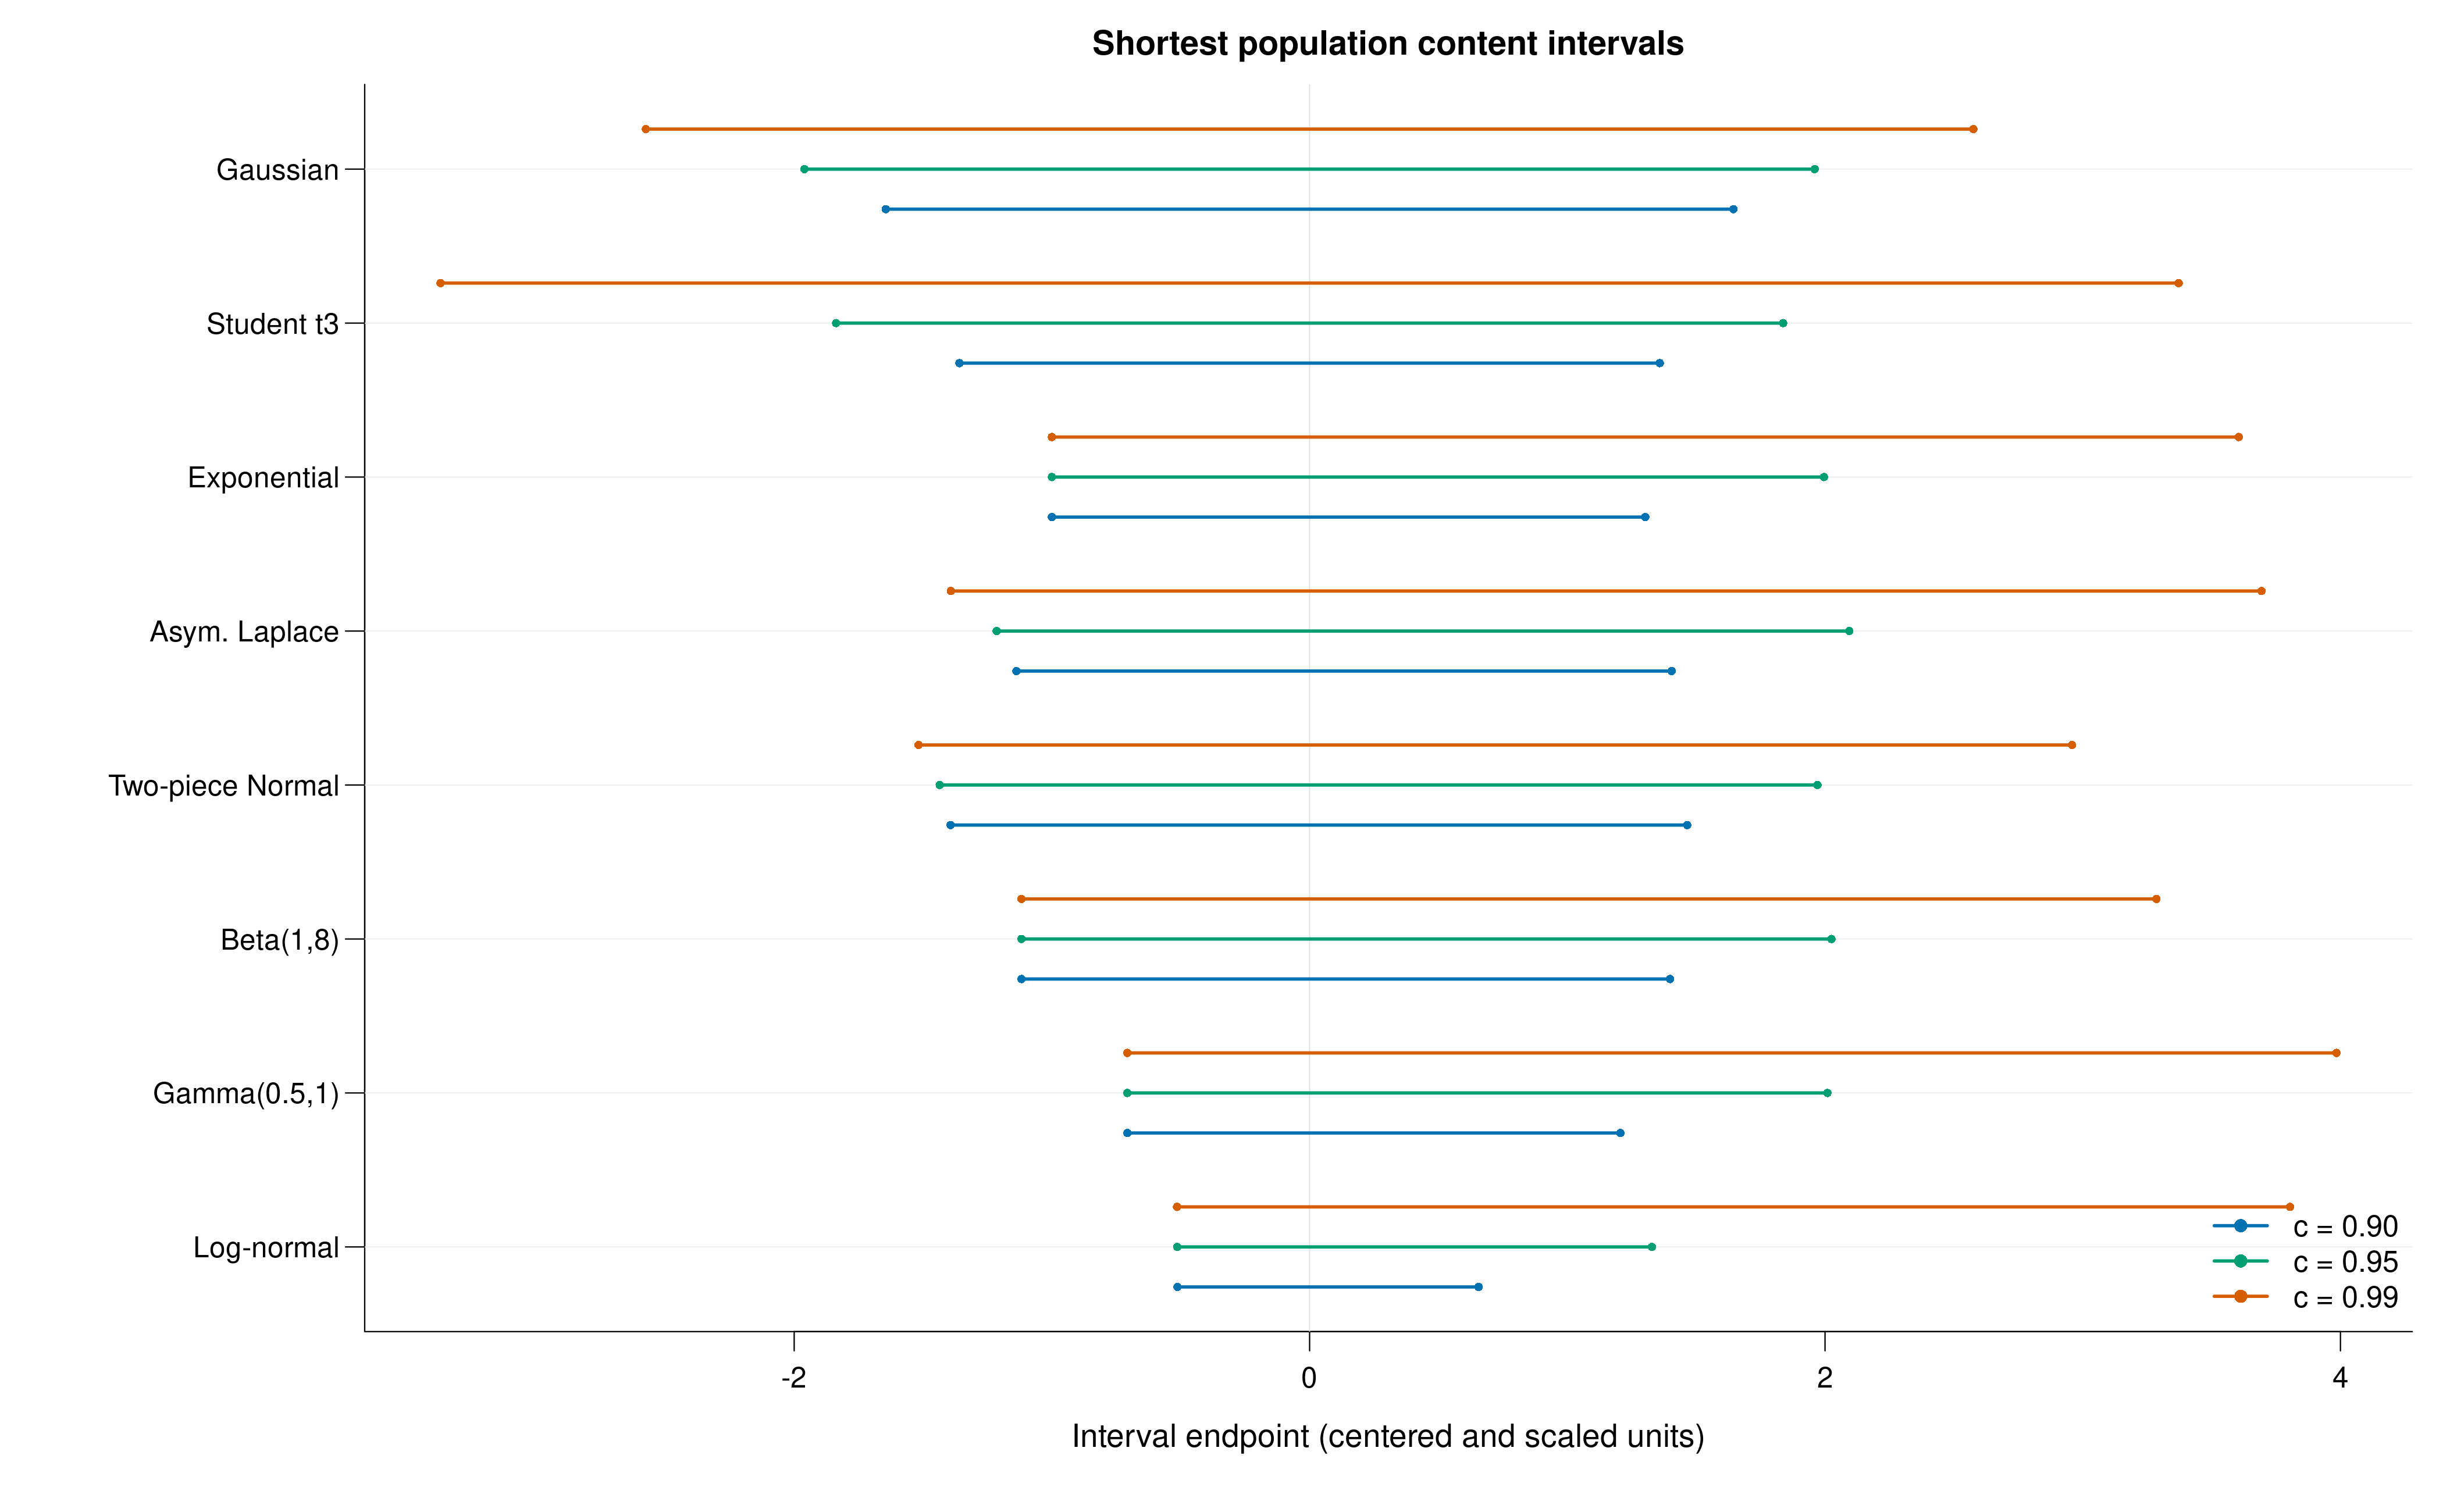
\includegraphics[width=\textwidth]{figures/ch05-mti/generated/figS03_tolerance_population_shortest_intervals.png}
\caption{\textbf{Population shortest-content intervals for the simulation
distributions.} Horizontal intervals show the shortest population content-\(c\)
intervals for the centered and scaled simulation laws. The figure supplies the
width benchmarks used to interpret the empirical width ranges in the main
article.}
\label{rqr2026:fig:supp-tolerance-population-shortest}
\end{figure}

These results provide empirical repeated-sampling evidence for the selected
profile rule. A distribution-free tolerance theorem for MTI remains to be
established.

\begin{table}[!htbp]
\centering
\caption{\textbf{Calibrated MTI probability cutoffs.} The lower bound is the smallest simultaneous one-sided calibration bound across eight distributions, with 24000 assessment samples per distribution. Validation ranges span the eight independent estimates.}\label{rqr2026:tab:supp-mti-profile-policy}
\TableStyle
\begin{tabular}{@{}rrrrr@{}}
\toprule
\(n\) & \(c\) & Cutoff \(\gamma\) & Calibration lower bound & Validation attainment (\%)\\
\midrule
50 & 0.90 & 0.987920 & 0.9595 & 96.1--98.0 \\
100 & 0.90 & 0.984112 & 0.9506 & 95.5--98.3 \\
100 & 0.95 & 0.987686 & 0.9556 & 95.6--97.3 \\
500 & 0.90 & 0.989746 & 0.9585 & 96.0--99.1 \\
500 & 0.95 & 0.991878 & 0.9643 & 97.1--98.9 \\
500 & 0.99 & 0.989553 & 0.9525 & 95.1--97.3 \\
1000 & 0.90 & 0.990729 & 0.9549 & 95.7--99.3 \\
1000 & 0.95 & 0.992002 & 0.9562 & 95.9--99.1 \\
1000 & 0.99 & 0.996684 & 0.9783 & 97.5--99.3 \\
\bottomrule
\end{tabular}
\end{table}


\paragraph{Scan reference for the fitted-content search.}
The reference retained count \(k\) is chosen before seeing the replicated
samples. For independent \(U_i\sim\mathrm{Unif}(0,1)\), define
\[
M_n(c)=\max_{0\le s\le1-c}\#\{i:U_i\in[s,s+c]\},\qquad
k_{n,c,\alpha}=\min\{k:\Pr(M_n(c)<k)\ge1-\alpha\}.
\]
For ordered observations \(Y_{(1)}\le\cdots\le Y_{(n)}\), the scan-reference
window is
\[
I^{\mathrm{ref}}_n=[Y_{(j_0)},Y_{(j_0+k-1)}],\qquad
j_0=\min\argmin_{1\le j\le n-k+1}\{Y_{(j+k-1)}-Y_{(j)}\}.
\]
This reference provides \(k/n\) for the initial fitted-content search.
The reported MTI endpoints are obtained from the selected profile fit.
Its fitted content can differ from
\(k/n\), and its interval does not inherit the scan reference's tolerance
argument.

Table~\ref{rqr2026:tab:supp-scan-reference} records the
retained counts, retained fractions, content buffers, and lower confidence
bounds used in the simulation design. Adaptive Clopper--Pearson calibration
selects the retained count for each feasible sample-size/content cell before
any distribution-specific replications are evaluated. The numerical calculation
adjusts one-sided Clopper--Pearson lower bounds over retained counts and
adaptive looks; numerical confidence is distinct from tolerance confidence.
The full-range probability is evaluated analytically. Exact evaluation of the
scan distribution remains a numerical problem.

When \(k=n\), the reference window is the full sample range. This occurs for
\((n,c)=(50,0.90),(100,0.95)\), and \((500,0.99)\). The MTI search still
uses fitted contents strictly below one, including fractional contents between
\((n-1)/n\) and one. The closed-window reference contains \(k\) observations
under continuity; the alternative half-open convention
\((Y_{(j)},Y_{(j+k)}]\) has different indices and requires its own calibration.

\begin{table}[H]
\centering
\caption{\textbf{Scan reference for the MTI fitted-content search.} The retained
count \(k\) is selected by adaptive Clopper--Pearson Monte Carlo scan
calibration. The content buffer is \(k/n-c\).}
\label{rqr2026:tab:supp-scan-reference}
\TableStyle
\begin{tabular}{@{}rrrrrr@{}}
\toprule
\(n\) & \(c\) & Retained count \(k\) & \(k/n\) & Buffer \(k/n-c\) & Lower confidence bound\\
\midrule
50 & 0.90 & 50 & 1.000 & 0.100 & 0.966 \\
100 & 0.90 & 98 & 0.980 & 0.080 & 0.979 \\
100 & 0.95 & 100 & 1.000 & 0.050 & 0.963 \\
500 & 0.90 & 467 & 0.934 & 0.034 & 0.950 \\
500 & 0.95 & 487 & 0.974 & 0.024 & 0.951 \\
500 & 0.99 & 500 & 1.000 & 0.010 & 0.960 \\
1000 & 0.90 & 925 & 0.925 & 0.025 & 0.960 \\
1000 & 0.95 & 968 & 0.968 & 0.018 & 0.958 \\
1000 & 0.99 & 998 & 0.998 & 0.008 & 0.975 \\
\bottomrule
\end{tabular}

\end{table}

Small-sample feasibility is governed by the full-range two-sided order-statistic
coverage probability
\[
  \Pr_F^n\{F(Y_{(n)})-F(Y_{(1)})\ge c\}
  =
  1-n(1-c)c^{n-1}-c^n .
\]
The smallest \(n\) satisfying this inequality depends on both content and
tolerance confidence. Table~\ref{rqr2026:tab:supp-full-range-thresholds} lists the
thresholds used to design the simulation study.

\begin{table}[H]
\centering
\caption{\textbf{Full-range feasibility thresholds.} Entries are the smallest
sample sizes for which the sample-range interval \([Y_{(1)},Y_{(n)}]\) reaches
the stated two-sided distribution-free content/confidence pair.}
\label{rqr2026:tab:supp-full-range-thresholds}
\TableStyle
\begin{tabular}{@{}lrrr@{}}
\toprule
Tolerance confidence & \(c=0.90\) & \(c=0.95\) & \(c=0.99\)\\
\midrule
\(0.90\) & 38 & 77 & 388\\
\(0.95\) & 46 & 93 & 473\\
\bottomrule
\end{tabular}
\end{table}

This distinction matters for interpreting the small sample sizes in
\citet{rqr-PourmohamadRichardsonSanso2026CalibratedBNP}. The values
\((38,77,388)\) are appropriate at \(90\%\) tolerance confidence. A
\(95\%\)-confidence design needs the larger thresholds \((46,93,473)\). The
simulation design therefore lists the feasible cells explicitly instead of
forming a Cartesian product of sample sizes and contents. This prevents the
comparison from treating structural infeasibility of the sample-bounded
order-statistic procedures as a method failure. It does not establish the
same feasibility boundary for the model-based MTI procedure.
The Young--Mathew comparator is evaluated through the \texttt{tolerance}
package's \texttt{nptol.int(..., method = "YM")} function. The completed
run used \texttt{tolerance} version 3.0.0, and the package version is included
in the method reproducibility record.

\subsection{Pharmaceutical Application Details}
\label{rqr2026:sec:supp-pharma-application}

\paragraph{Data and paired partitions.}
The application uses the manufacturing data described by
\citet{rqr-ZagarMihelic2022PharmaManufacturing} and version 1 of the public
\texttt{Laboratory.csv} file \citep{rqr-ZagarMihelic2021LaboratoryCsv}. The source
contains \PharmaRawBatches{} batches and \PharmaRawFields{} recorded fields.
File size, MD5, and SHA256 are verified before extracting product code
\PharmaProductCode{}, which gives \PharmaBatches{} batches. The main response
is the reported film-coated-tablet tensile metric. Tablet-core
weight relative standard deviation (RSD) provides a more asymmetric
supplementary example. The recorded active pharmaceutical ingredient (API)
batch identifier defines one grouping used below. The file contains ties,
and the batch records may be dependent.

The source defines tensile strength using average hardness and maximum tablet
dimensions. Its numerical values reproduce from these batch summaries using
\(3.14\) in place of \(\pi\), to rounding precision. This ratio of summaries
need not equal the average of tablet-specific tensile strengths. In product
code \PharmaProductCode{}, \PharmaFctHardnessQuestions{} film-coated average
hardness values exceed their recorded maxima, and
\PharmaCoreHardnessQuestions{} core averages fall below their recorded minima.
If the summaries concern the same tablets, units, and measurement window,
these orderings are inconsistent. The public definitions do not establish
those conditions. We preserve all values and treat the derived response's
physical interpretation as unresolved. The source describes in-specification
historical variation and excludes batches without final quality results;
these records do not represent every attempted production batch.

\begin{table}[H]
\centering
\caption{\textbf{Response diagnostics for product code \PharmaProductCode{}.}
The reported tensile metric is used in the main article. Weight RSD has a
stronger asymmetric-placement interpretation. Film-coated-tablet hardness has
more ties and is excluded.}
\label{rqr2026:tab:supp-pharma-response-diagnostics}
\TableStyle
\setlength{\tabcolsep}{2pt}\begin{tabular}{@{}llrrrrrr@{}}
\toprule
Role & Response & Batches & Distinct & Largest tie & Median & SD & Skewness\\
\midrule
Main & fct\_tensile & 187 & 82 & 11 & 1.341 & 0.124 & 0.44 \\
Supplement & tbl\_rsd\_weight & 187 & 83 & 6 & 1.030 & 0.467 & 3.00 \\
Excluded & fct\_av\_hardness & 187 & 32 & 17 & 70.560 & 6.459 & 0.48 \\
\bottomrule
\end{tabular}

\end{table}

For each primary random split, every method uses the same \PharmaTrain{}
training batches and \PharmaHeldout{} withheld batches. The two responses use
identical partitions. Each split is generated from its recorded seed; changing
worker order leaves its membership unchanged. The requested population
content is \(c=\PharmaContent\), and nominal tolerance confidence is
\(\PharmaConfidence\). The selected MTI rule uses posterior content
probability threshold \(\PharmaScreen\) and internal retained-count reference
\(k=\PharmaRetained\). This internal calibration anchor is used to construct
the fitted-content search. Fitted content and tilt vary within each sample
under the preassigned rule; fitting settings and the calibration rule are
unchanged across responses and partitions.

\paragraph{Representative split.}
The displayed intervals come from an actual random split chosen separately
for each response by a prespecified median-distance rule. For every split in
which all three methods return intervals, collect each method's lower and
upper endpoints, width, held-out empirical content, and two tail-omission
fractions as components \(x_{sj}\). Let \(m_j\) be the across-split median
of component \(j\), and let \(d_j\) be its median absolute deviation (MAD). A zero
MAD is replaced by the interquartile range; a remaining zero scale is replaced
by one. The selected split minimizes
\[
  \sum_j \left\{(x_{sj}-m_j)/d_j\right\}^2,
\]
with ties resolved by the smallest split identifier. Training and held-out
indices and the selection score are retained with the results. This rule
selects split \PharmaTensileRepresentative{} for the tensile metric and
split \PharmaRsdRepresentative{} for weight RSD.

\paragraph{Interval placement for weight RSD.}
The RSD response has sample skewness \PharmaRsdSkewness{}. MTI has median
width \PharmaRsdMtiWidth{}, compared with \PharmaRsdYmWidth{} for
Young--Mathew and \PharmaRsdWilksWidth{} for Wilks. The median paired width
difference against Young--Mathew is \PharmaRsdPairedYmWidthDifference{}.
The tail allocation explains part of this difference: MTI omits median
fractions \PharmaRsdMtiLowerOmitted\% below and
\PharmaRsdMtiUpperOmitted\% above, while Young--Mathew omits
\PharmaRsdYmLowerOmitted\% and \PharmaRsdYmUpperOmitted\%, respectively.
A shorter interval can exclude more of the scientifically adverse upper
tail. An upper one-sided tolerance limit would be more natural for a direct
quality-control decision; the present two-sided analysis describes placement
on the historical data.

\begin{table}[H]
\centering
\caption{\textbf{Weight-RSD application.} Intervals use \PharmaTrain{}
training and \PharmaHeldout{} held-out batches over \PharmaSplits{} paired
random splits. Bracketed ranges are empirical 2.5\%--97.5\% quantiles.
Held-out \(\ge c\) is the percentage of all splits with empirical content at
least \(c\). The splits reuse one finite dataset and are not independent
sampling replications.}
\label{rqr2026:tab:supp-pharma-rsd}
\TableStyle
\begin{tabularx}{\textwidth}{@{}lrr>{\raggedright\arraybackslash}X>{\raggedright\arraybackslash}X@{}}
\toprule
Method & Splits & Returned (\%) & Median lower/upper & Width median [95\% range]\\
\midrule
MTI (proposed) & 1000 & 100.0 & 0.610 / 2.300 & 1.690 [1.260, 2.220] \\
Young--Mathew (benchmark) & 1000 & 100.0 & 0.700 / 2.970 & 2.262 [1.572, 2.597] \\
Wilks (benchmark) & 1000 & 100.0 & 0.600 / 4.050 & 3.400 [2.000, 3.450] \\
\bottomrule
\end{tabularx}
\par\smallskip
\begin{tabularx}{\textwidth}{@{}l>{\raggedright\arraybackslash}Xrr@{}}
\toprule
Method & Held-out content median [95\% range] (\%) & Held-out $\ge c$ (\%) & Omitted below/above (\%)\\
\midrule
MTI & 95.4 [88.5, 100.0] & 90.6 & 1.1 / 3.4 \\
Young--Mathew & 95.4 [87.4, 100.0] & 87.9 & 3.4 / 1.1 \\
Wilks & 98.9 [93.1, 100.0] & 99.3 & 0.0 / 0.0 \\
\bottomrule
\end{tabularx}

\end{table}

\begin{figure}[H]
\centering
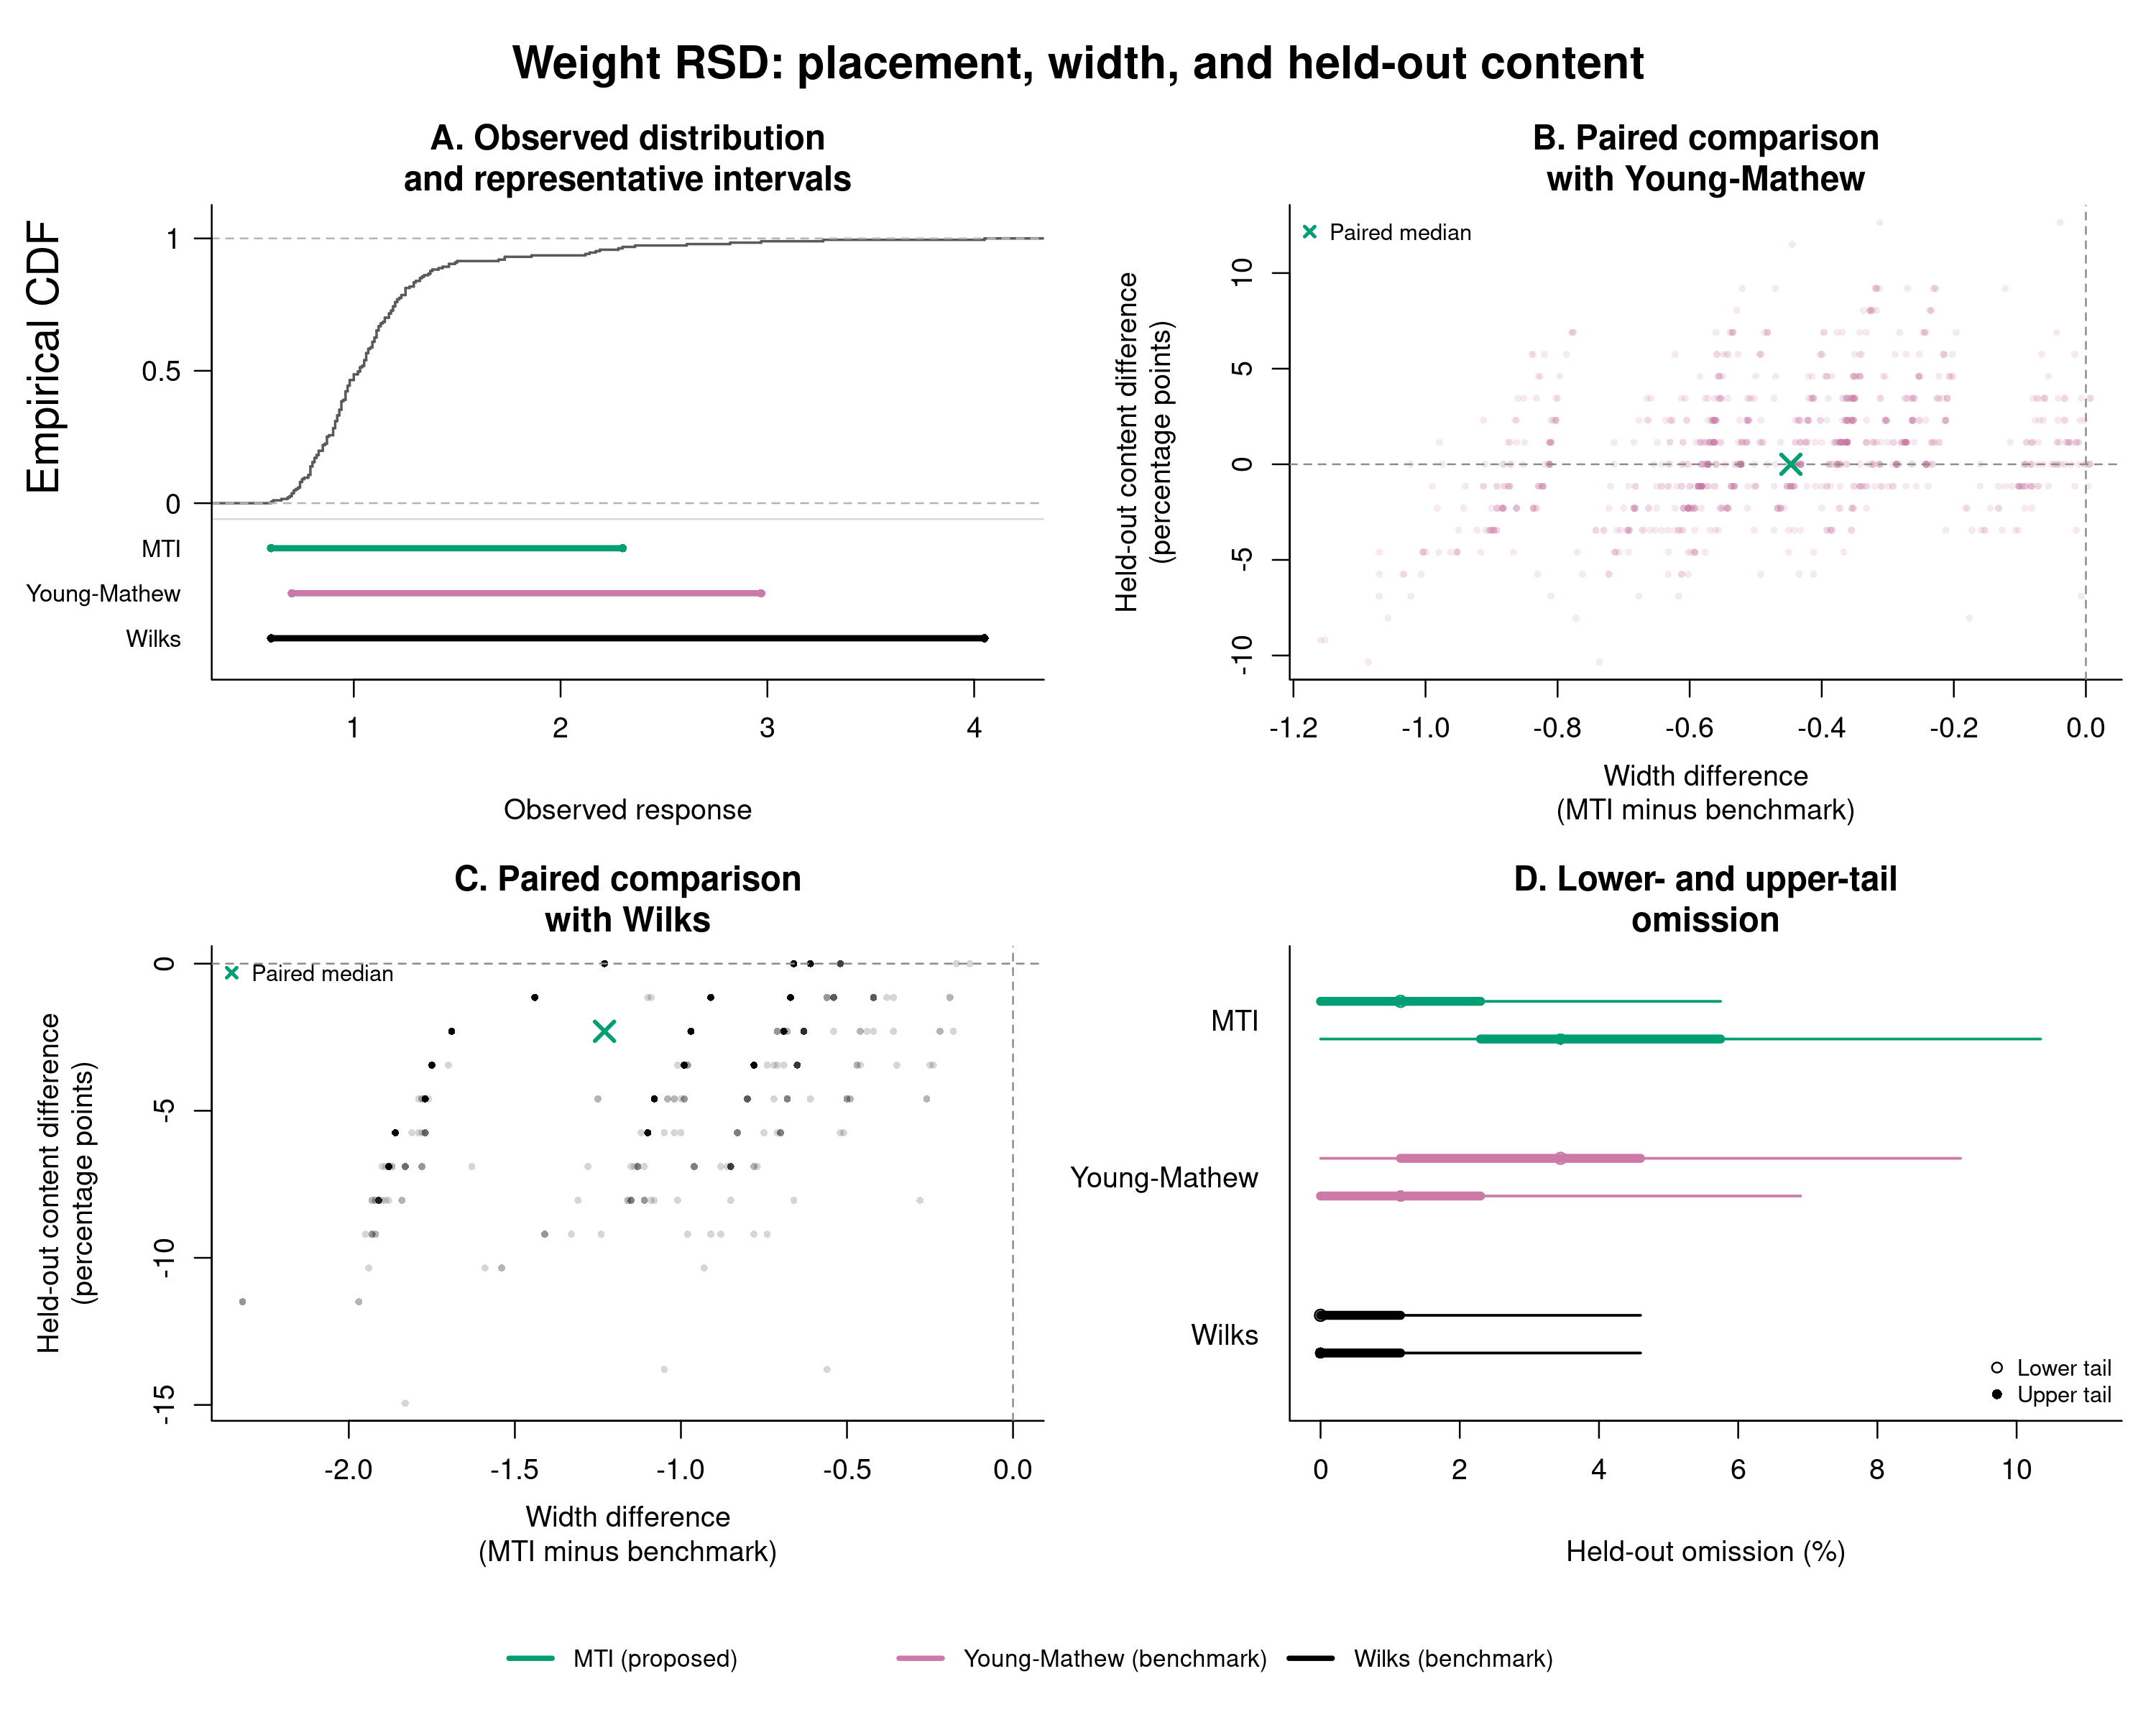
\includegraphics[width=\textwidth]{figures/ch05-mti/generated/figS04_pharma_application_rsd_intervals.png}
\caption{\textbf{Interval placement and held-out comparisons for weight RSD.}
The panels follow the main application figure. The representative split
\PharmaRsdRepresentative{} is selected by the same median-distance rule.
Thick and thin tail-omission segments show interquartile and empirical 95\%
ranges, with median markers. The response is strongly right-skewed, but an
upper one-sided tolerance limit would be more natural for a direct
quality-control decision.}
\label{rqr2026:fig:supp-pharma-rsd}
\end{figure}

The paired comparisons below use MTI minus the named benchmark for endpoint,
width, content, and omission differences. The width ratio divides MTI
width by benchmark width. They summarize the observed paired split
distributions without treating overlapping splits as independent observations.

\begingroup
\footnotesize
\setlength{\tabcolsep}{3pt}
\begin{longtable}{@{}llrrrr@{}}
\caption{\textbf{Paired comparisons for Reported tensile metric.} Differences are MTI minus the benchmark; the width ratio divides the corresponding widths. Content and omission differences are percentage points. Entries describe paired random splits of one finite dataset. IQR is the interquartile range.}\label{rqr2026:tab:supp-pharma-primary-paired}\\
\toprule
Quantity & Benchmark & Pairs & Median & IQR & 95\% range\\
\midrule
\endfirsthead
\toprule
Quantity & Benchmark & Pairs & Median & IQR & 95\% range\\
\midrule
\endhead
Width difference & Young--Mathew & 1000 & -0.014 & 0.033 & [-0.076, 0.013] \\
Width ratio & Young--Mathew & 1000 & 0.973 & 0.062 & [0.862, 1.023] \\
Lower-endpoint difference & Young--Mathew & 1000 & -0.020 & 0.043 & [-0.080, 0.055] \\
Upper-endpoint difference & Young--Mathew & 1000 & -0.039 & 0.074 & [-0.114, 0.048] \\
Held-out content difference & Young--Mathew & 1000 & 0.000 & 2.299 & [-6.897, 3.448] \\
Lower-omission difference & Young--Mathew & 1000 & 0.000 & 1.149 & [-4.598, 4.598] \\
Upper-omission difference & Young--Mathew & 1000 & 1.149 & 2.299 & [-1.149, 6.897] \\
\addlinespace
Width difference & Wilks & 1000 & -0.135 & 0.050 & [-0.226, -0.087] \\
Width ratio & Wilks & 1000 & 0.791 & 0.063 & [0.674, 0.859] \\
Lower-endpoint difference & Wilks & 1000 & 0.042 & 0.061 & [0.000, 0.116] \\
Upper-endpoint difference & Wilks & 1000 & -0.094 & 0.058 & [-0.188, 0.000] \\
Held-out content difference & Wilks & 1000 & -3.448 & 2.299 & [-9.952, 0.000] \\
Lower-omission difference & Wilks & 1000 & 0.000 & 2.299 & [0.000, 6.897] \\
Upper-omission difference & Wilks & 1000 & 2.299 & 2.299 & [0.000, 8.046] \\
\addlinespace
\bottomrule
\end{longtable}
\endgroup

\begingroup
\footnotesize
\setlength{\tabcolsep}{3pt}
\begin{longtable}{@{}llrrrr@{}}
\caption{\textbf{Paired comparisons for Weight RSD.} Differences are MTI minus the benchmark; the width ratio divides the corresponding widths. Content and omission differences are percentage points. Entries describe paired random splits of one finite dataset. IQR is the interquartile range.}\label{rqr2026:tab:supp-pharma-rsd-paired}\\
\toprule
Quantity & Benchmark & Pairs & Median & IQR & 95\% range\\
\midrule
\endfirsthead
\toprule
Quantity & Benchmark & Pairs & Median & IQR & 95\% range\\
\midrule
\endhead
Width difference & Young--Mathew & 1000 & -0.447 & 0.281 & [-0.951, -0.027] \\
Width ratio & Young--Mathew & 1000 & 0.785 & 0.128 & [0.629, 0.983] \\
Lower-endpoint difference & Young--Mathew & 1000 & -0.088 & 0.040 & [-0.131, -0.010] \\
Upper-endpoint difference & Young--Mathew & 1000 & -0.520 & 0.250 & [-1.080, -0.067] \\
Held-out content difference & Young--Mathew & 1000 & 0.000 & 3.448 & [-5.747, 8.046] \\
Lower-omission difference & Young--Mathew & 1000 & -2.299 & 2.299 & [-9.195, 0.000] \\
Upper-omission difference & Young--Mathew & 1000 & 1.149 & 3.448 & [0.000, 6.897] \\
\addlinespace
Width difference & Wilks & 1000 & -1.230 & 0.780 & [-1.910, -0.460] \\
Width ratio & Wilks & 1000 & 0.586 & 0.156 & [0.444, 0.766] \\
Lower-endpoint difference & Wilks & 1000 & 0.000 & 0.000 & [0.000, 0.080] \\
Upper-endpoint difference & Wilks & 1000 & -1.230 & 0.780 & [-1.880, -0.420] \\
Held-out content difference & Wilks & 1000 & -2.299 & 3.448 & [-9.195, 0.000] \\
Lower-omission difference & Wilks & 1000 & 0.000 & 0.000 & [0.000, 3.056] \\
Upper-omission difference & Wilks & 1000 & 2.299 & 3.448 & [0.000, 8.046] \\
\addlinespace
\bottomrule
\end{longtable}
\endgroup


\paragraph{Partition sensitivities.}
Forward recorded order trains on the first \PharmaTrain{} batches in recorded
batch order, with original row order breaking ties, and holds out the final
\PharmaHeldout{}. Reverse recorded order trains on the final \PharmaTrain{} and
holds out the first \PharmaHeldout{}. Each is a single labeled partition.
Production-month and API-batch sensitivities keep whole groups on one side of
the training boundary. Response-independent allocation conditional on exactly
\PharmaTrain{} training batches gives up to \PharmaGroupedSplits{} unique
partitions for each grouping. Fixed seeds and removal of duplicate
partitions determine the reported sets before fitting. Exact training size
preserves the sample-size cell of the fixed calibration rule.
These orderings use batch identifiers and source rows. Ambiguous process date
strings and unresolved relationships between production stages prevent a
verified calendar interpretation.

Tables~\ref{rqr2026:tab:supp-pharma-primary-sensitivity}
and~\ref{rqr2026:tab:supp-pharma-rsd-sensitivity} give actual split counts and
summaries for each design. The recorded-order cases show that partition choice
can materially change held-out empirical content. For MTI, reverse
order gives tensile-metric content \PharmaTensileReverseContent\%;
forward order gives RSD content \PharmaRsdForwardContent\%.
These comparisons describe variation across the recorded batches and are
insufficient to distinguish dependence from changes in the batch distribution.

\begingroup
\footnotesize
\setlength{\tabcolsep}{2.5pt}
\begin{longtable}{@{}lrrrrr@{}}
\caption{\textbf{Partition sensitivities for Reported tensile metric.} Each heading gives the number of splits and median training/held-out sizes. Width, content, and omissions are medians within the labeled design. Content, attainment, omissions, and return rates are percentages. The recorded-order cases each contain one partition.}\label{rqr2026:tab:supp-pharma-primary-sensitivity}\\
\toprule
Method & Width & \shortstack{Held-out\\content} & \shortstack{Held-out\\$\ge c$} & \shortstack{Omitted\\below/above} & Returned\\
\midrule
\endfirsthead
\toprule
Method & Width & \shortstack{Held-out\\content} & \shortstack{Held-out\\$\ge c$} & \shortstack{Omitted\\below/above} & Returned\\
\midrule
\endhead
\multicolumn{6}{@{}l}{\textit{Random splits: 1000 splits; training/held-out 100/87}}\\
MTI & 0.514 & 95.4 & 88.0 & 1.1 / 2.3 & 100.0 \\
Young--Mathew & 0.533 & 95.4 & 91.9 & 2.3 / 1.1 & 100.0 \\
Wilks & 0.665 & 98.9 & 99.3 & 0.0 / 0.0 & 100.0 \\
\addlinespace
\multicolumn{6}{@{}l}{\textit{Forward recorded order: 1 splits; training/held-out 100/87}}\\
MTI & 0.517 & 96.6 & 100.0 & 1.1 / 2.3 & 100.0 \\
Young--Mathew & 0.528 & 96.6 & 100.0 & 1.1 / 2.3 & 100.0 \\
Wilks & 0.708 & 100.0 & 100.0 & 0.0 / 0.0 & 100.0 \\
\addlinespace
\multicolumn{6}{@{}l}{\textit{Reverse recorded order: 1 splits; training/held-out 100/87}}\\
MTI & 0.459 & 89.7 & 0.0 & 6.9 / 3.4 & 100.0 \\
Young--Mathew & 0.499 & 87.4 & 0.0 & 11.5 / 1.1 & 100.0 \\
Wilks & 0.628 & 97.7 & 100.0 & 1.1 / 1.1 & 100.0 \\
\addlinespace
\multicolumn{6}{@{}l}{\textit{Production-month groups: 250 splits; training/held-out 100/87}}\\
MTI & 0.514 & 94.3 & 78.8 & 1.1 / 2.3 & 100.0 \\
Young--Mathew & 0.520 & 94.3 & 72.0 & 2.3 / 1.1 & 100.0 \\
Wilks & 0.665 & 98.9 & 94.4 & 0.0 / 0.0 & 100.0 \\
\addlinespace
\multicolumn{6}{@{}l}{\textit{API-batch groups: 250 splits; training/held-out 100/87}}\\
MTI & 0.514 & 94.3 & 75.6 & 1.1 / 3.4 & 100.0 \\
Young--Mathew & 0.526 & 94.8 & 79.2 & 1.1 / 1.1 & 100.0 \\
Wilks & 0.665 & 98.9 & 96.4 & 0.0 / 0.0 & 100.0 \\
\addlinespace
\bottomrule
\end{longtable}
\endgroup

\begingroup
\footnotesize
\setlength{\tabcolsep}{2.5pt}
\begin{longtable}{@{}lrrrrr@{}}
\caption{\textbf{Partition sensitivities for Weight RSD.} Each heading gives the number of splits and median training/held-out sizes. Width, content, and omissions are medians within the labeled design. Content, attainment, omissions, and return rates are percentages. The recorded-order cases each contain one partition.}\label{rqr2026:tab:supp-pharma-rsd-sensitivity}\\
\toprule
Method & Width & \shortstack{Held-out\\content} & \shortstack{Held-out\\$\ge c$} & \shortstack{Omitted\\below/above} & Returned\\
\midrule
\endfirsthead
\toprule
Method & Width & \shortstack{Held-out\\content} & \shortstack{Held-out\\$\ge c$} & \shortstack{Omitted\\below/above} & Returned\\
\midrule
\endhead
\multicolumn{6}{@{}l}{\textit{Random splits: 1000 splits; training/held-out 100/87}}\\
MTI & 1.690 & 95.4 & 90.6 & 1.1 / 3.4 & 100.0 \\
Young--Mathew & 2.262 & 95.4 & 87.9 & 3.4 / 1.1 & 100.0 \\
Wilks & 3.400 & 98.9 & 99.3 & 0.0 / 0.0 & 100.0 \\
\addlinespace
\multicolumn{6}{@{}l}{\textit{Forward recorded order: 1 splits; training/held-out 100/87}}\\
MTI & 1.090 & 85.1 & 0.0 & 1.1 / 13.8 & 100.0 \\
Young--Mathew & 1.452 & 83.9 & 0.0 & 6.9 / 9.2 & 100.0 \\
Wilks & 2.660 & 97.7 & 100.0 & 1.1 / 1.1 & 100.0 \\
\addlinespace
\multicolumn{6}{@{}l}{\textit{Reverse recorded order: 1 splits; training/held-out 100/87}}\\
MTI & 2.010 & 98.9 & 100.0 & 0.0 / 1.1 & 100.0 \\
Young--Mathew & 2.272 & 96.6 & 100.0 & 2.3 / 1.1 & 100.0 \\
Wilks & 3.450 & 100.0 & 100.0 & 0.0 / 0.0 & 100.0 \\
\addlinespace
\multicolumn{6}{@{}l}{\textit{Production-month groups: 250 splits; training/held-out 100/87}}\\
MTI & 1.760 & 96.6 & 66.4 & 1.1 / 2.3 & 100.0 \\
Young--Mathew & 2.261 & 92.0 & 62.4 & 2.3 / 1.1 & 100.0 \\
Wilks & 3.400 & 98.9 & 95.2 & 0.0 / 0.0 & 100.0 \\
\addlinespace
\multicolumn{6}{@{}l}{\textit{API-batch groups: 250 splits; training/held-out 100/87}}\\
MTI & 1.710 & 95.4 & 83.6 & 0.0 / 2.3 & 100.0 \\
Young--Mathew & 2.263 & 95.4 & 83.2 & 3.4 / 1.1 & 100.0 \\
Wilks & 3.400 & 98.9 & 98.8 & 0.0 / 0.0 & 100.0 \\
\addlinespace
\bottomrule
\end{longtable}
\endgroup


\begin{figure}[H]
\centering
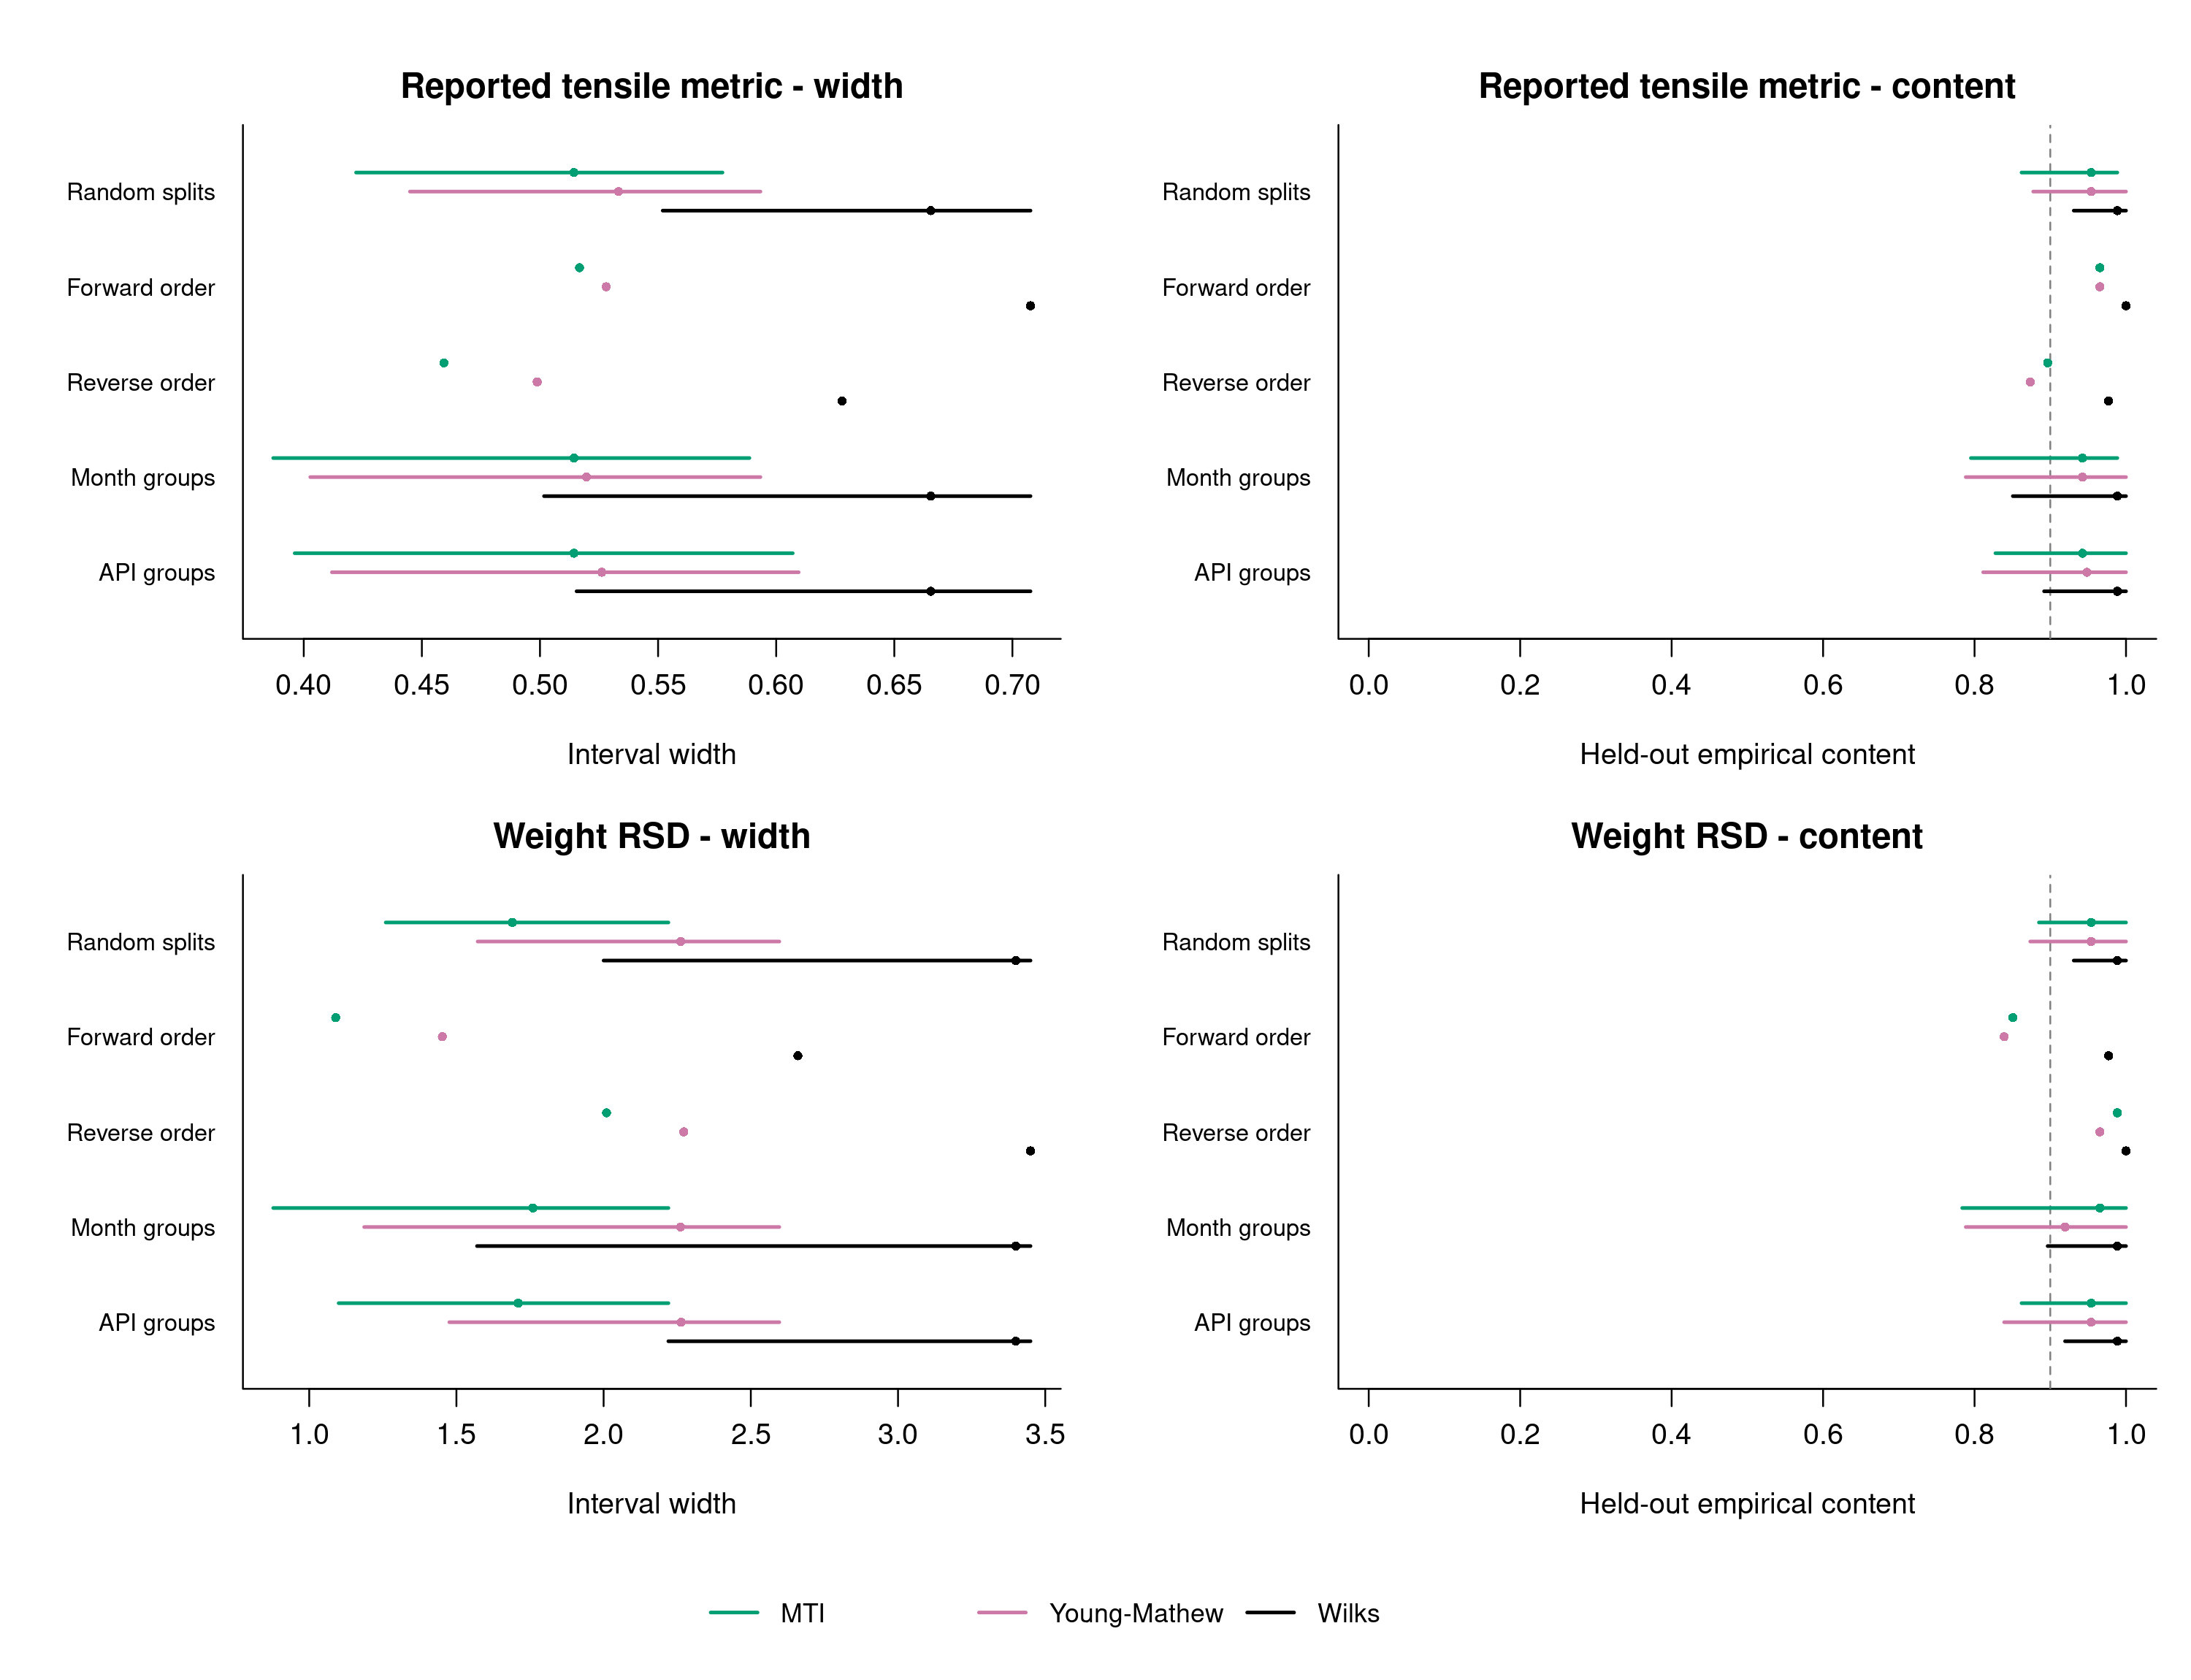
\includegraphics[width=\textwidth]{figures/ch05-mti/generated/figS05_pharma_application_partition_sensitivity.png}
\caption{\textbf{Sensitivity to training and held-out partitions.} Points show
median widths or held-out empirical content within each labeled design.
Segments give empirical 95\% ranges for random and grouped splits. The two
recorded-order designs each contain one partition and are shown as individual
points. Dashed lines mark the requested content \(c=\PharmaContent\).
The plots describe historical partition sensitivity.}
\label{rqr2026:fig:supp-pharma-partition-sensitivity}
\end{figure}

\paragraph{Production campaigns.}
The associated process archive \citep{rqr-ZagarMihelic2021Process} maps all
\PharmaBatches{} batches uniquely to \PharmaCampaigns{} manufacturing
campaigns, containing 2--12 batches each. Campaigns can cross recorded months
and share API lots. Every random partition shares campaigns; the median number
of withheld batches in represented campaigns is
\PharmaRandomSharedHeldout{} of \PharmaHeldout{}. This identifies the
production groups represented on both sides, without establishing either
dependence or independence.

As a retrospective sensitivity, we retain every existing month-grouped
partition with no shared campaign. This response-independent criterion selects
\PharmaCampaignDisjointMonths{} partitions; all \PharmaGroupedSplits{} original
month partitions remain in the comparison. Table~\ref{rqr2026:tab:supp-pharma-campaign}
reports the corresponding widths, empirical content, and omissions together.
For MTI the selected subset has median held-out content
\PharmaCampaignTensileContent\% for the tensile metric and
\PharmaCampaignRsdContent\% for RSD. These are overlapping partitions of one
historical dataset. Moreover, \PharmaCampaignDisjointApiShared{} selected
partitions still share API lots. Their content-attainment frequencies do not
estimate nominal tolerance confidence or isolate a causal campaign effect.

\begin{table}[H]
\centering
\caption{\textbf{Retrospective sensitivity to campaign sharing.} Both sets
use existing month-grouped partitions with \PharmaTrain{} training and
\PharmaHeldout{} withheld batches; no intervals are refitted. Brackets give
empirical 2.5\%--97.5\% width quantiles. Content is median held-out empirical
content; \(\ge c\) is the percentage of partitions meeting the requested
content. Below/above gives median omitted fractions. Content, attainment, and
omissions are percentages.
The subset is retrospective and the partitions are not independent samples.}
\label{rqr2026:tab:supp-pharma-campaign}
\begingroup
\footnotesize
\setlength{\tabcolsep}{3pt}
\begin{tabularx}{\textwidth}{@{}l>{\raggedright\arraybackslash}Xrrr@{}}
\toprule
Method & Width median [95\% range] & Content & $\ge c$ & Below/above\\
\midrule
\multicolumn{5}{@{}l}{\textit{Reported tensile metric: all month partitions (250)}}\\
MTI & 0.514 [0.387, 0.589] & 94.3 & 78.8 & 1.1/2.3 \\
Young--Mathew & 0.520 [0.403, 0.593] & 94.3 & 72.0 & 2.3/1.1 \\
Wilks & 0.665 [0.502, 0.708] & 98.9 & 94.4 & 0.0/0.0 \\
\addlinespace
\multicolumn{5}{@{}l}{\textit{Reported tensile metric: no shared campaign (63)}}\\
MTI & 0.483 [0.381, 0.555] & 92.0 & 71.4 & 1.1/3.4 \\
Young--Mathew & 0.515 [0.419, 0.590] & 93.1 & 68.3 & 2.3/1.1 \\
Wilks & 0.649 [0.525, 0.708] & 97.7 & 92.1 & 0.0/1.1 \\
\addlinespace
\multicolumn{5}{@{}l}{\textit{Weight RSD: all month partitions (250)}}\\
MTI & 1.760 [0.878, 2.220] & 96.6 & 66.4 & 1.1/2.3 \\
Young--Mathew & 2.261 [1.187, 2.597] & 92.0 & 62.4 & 2.3/1.1 \\
Wilks & 3.400 [1.570, 3.450] & 98.9 & 95.2 & 0.0/0.0 \\
\addlinespace
\multicolumn{5}{@{}l}{\textit{Weight RSD: no shared campaign (63)}}\\
MTI & 1.670 [0.700, 2.211] & 92.0 & 55.6 & 1.1/2.3 \\
Young--Mathew & 2.220 [1.136, 2.576] & 92.0 & 60.3 & 2.3/1.1 \\
Wilks & 3.260 [1.567, 3.450] & 97.7 & 95.2 & 1.1/0.0 \\
\addlinespace
\bottomrule
\end{tabularx}
\endgroup

\end{table}

\paragraph{Numerical diagnostics.}
Every selected MTI fit retains its content, tilt, posterior content
probability, candidate counts, profile iterations, and relative objective gap.
All candidate fits must satisfy the objective-gap tolerance
\(\PharmaObjectiveTolerance\) before the interval is selected. The
selected-fit numerical criterion is met in \PharmaTensileConverged{} of
\PharmaTensileReturned{} returned tensile-metric fits and
\PharmaRsdConverged{} of \PharmaRsdReturned{} returned RSD fits.
The main summaries retain every split. Independent recalculation verifies
all 3004 selected fixed-target profiles, posterior content probabilities,
and held-out contents; comparator intervals agree with the original analysis
on the same observations. These numerical checks concern the computed
criterion and do not remove the application limitations from overlapping
partitions, ties, and possible dependence.

\begin{table}[H]
\centering
\caption{\textbf{MTI numerical diagnostics for primary random splits.}
Numerical summaries are medians with empirical 95\% ranges among returned
fits. Return counts and the convergence flag are reported separately.}
\label{rqr2026:tab:supp-pharma-numerical}
\TableStyle
\begin{tabularx}{\textwidth}{@{}ll>{\raggedright\arraybackslash}X@{}}
\toprule
Response & Diagnostic & Summary\\
\midrule
Reported tensile metric & Returned / all splits & 1000 / 1000 \\
 & Convergence flag / returned & 1000 / 1000 (100.0\%) \\
 & Candidates evaluated & 106 [103, 107] \\
 & Eligible candidates & 88.0 [85.0, 91.0] \\
 & Selected fitted content & 0.9600 [0.9450, 0.9600] \\
 & Selected tilt & -0.0030 [-0.0109, 0.0066] \\
 & Posterior content probability & 0.9926 [0.9925, 0.9927] \\
 & Profile iterations & 59.0000 [55.0000, 60.0000] \\
 & Absolute relative objective gap & 1.90e-14 [6.17e-16, 6.17e-14] \\
\addlinespace
Weight RSD & Returned / all splits & 1000 / 1000 \\
 & Convergence flag / returned & 1000 / 1000 (100.0\%) \\
 & Candidates evaluated & 103 [103, 105] \\
 & Eligible candidates & 85.0 [85.0, 91.0] \\
 & Selected fitted content & 0.9600 [0.9600, 0.9600] \\
 & Selected tilt & -0.0572 [-0.0704, -0.0313] \\
 & Posterior content probability & 0.9936 [0.9933, 0.9939] \\
 & Profile iterations & 60.0000 [56.0000, 61.0000] \\
 & Absolute relative objective gap & 1.40e-15 [1.07e-16, 5.31e-15] \\
\addlinespace
\bottomrule
\end{tabularx}

\end{table}

Failed interval calculations, if any, remain in the results and count as
nonattainment; endpoint and width summaries condition on interval return.
The recorded posterior content probability is a calculation under the DP
model. Held-out empirical content is evaluated on finite withheld batches,
and the nominal tolerance-confidence assessment remains the separate
simulation study.

\subsection{Reproducibility and Validation Limits}
\label{rqr2026:sec:supp-reproducibility}

The reproducibility materials separate mathematical statements, numerical
construction, and repeated-sampling evidence. The proofs above support the
population MPI and MTI identities, the fractional empirical score balance, and
the direct DP fixed-interval content law under their stated assumptions. The
scan-reference retained counts are calibrated before the replicated samples are analyzed.
The MTI content-probability cutoff is selected in a separate
calibration run and then applied unchanged in the independent validation run.

The validation evidence is confined to iid continuous univariate samples from
the prespecified simulation distributions. It does not establish tolerance
validity for regression intervals, dynamic endpoint states, dependent samples,
or response-predictive distributions. Those extensions require their own
targets, assumptions, algorithms, diagnostics, and validation designs.
\section{Regression and dynamic endpoint computation}
\subsection{Notation and Targets}
\label{mti:sec:supp-targets}

For an observation \(y_i\) and raw roots \(\eta_{1i}\) and \(\eta_{2i}\),
define
\[
e_i=(y_i-\eta_{1i})(y_i-\eta_{2i}),\qquad
\rho_c(r)=r\{c-\ind(r<0)\}.
\]
The MPI loss is \(\rho_c(e_i)\). With fixed tilt \(\delta_i\), the MTI loss is
\[
\rho_c(e_i)-c\delta_i(\eta_{1i}+\eta_{2i}-2y_i).
\]
The cumulative loss over observed indices \(I_{\mathrm{obs}}\) is denoted by
\(L_{c,\delta}(\theta)\). The fixed-target generalized posterior is
\[
\pi(\theta\mid D)
\propto
\exp\{-\omega_{\mathrm R}L_{c,\delta}(\theta)\}\pi_0(\theta).
\]
The symbols \(c\), \(\delta\), and \(\omega_{\mathrm R}\) have different roles:
content, retained-mean tilt, and learning rate, respectively.

\subsection{Root Labels and Endpoint Summaries}
\label{mti:sec:supp-labels}

The product-residual loss is invariant to exchanging the two raw roots. With
exchangeable root priors, the unordered pair is identified but the labels
``root 1'' and ``root 2'' are not. Endpoint summaries are therefore computed
after sorting the roots at the evaluation points:
\[
L_i=\min(\eta_{1i},\eta_{2i}),\qquad
U_i=\max(\eta_{1i},\eta_{2i}),\qquad
W_i=U_i-L_i.
\]

For static linear roots, define
\[
\beta_m=\frac{\beta_1+\beta_2}{2},\qquad
\beta_s=\frac{\beta_2-\beta_1}{2}.
\]
Then \(M(x)=x^\top\beta_m\), \(S(x)=x^\top\beta_s\), and
\[
L(x)=M(x)-|S(x)|,\qquad
U(x)=M(x)+|S(x)|,\qquad
W(x)=2|S(x)|.
\]
The midpoint coefficient \(\beta_m\) is root-label invariant. The signed gap
coefficient \(\beta_s\) changes sign under a root swap. Lower- and
upper-endpoint coefficient summaries require a declared design region where the
two roots remain ordered.

\subsection{Pseudo-AL Augmentation}
\label{mti:sec:supp-pseudo-al}

Let
\[
\sigma_{\mathrm R}=\omega_{\mathrm R}^{-1},\qquad
\xi_c=\frac{1-2c}{c(1-c)},\qquad
\phi_c=\frac{2}{c(1-c)}.
\]
The single-observation loss factor satisfies
\begin{align}
&\frac{c(1-c)}{\sigma_{\mathrm R}}
\exp\{-\rho_c(e_i)/\sigma_{\mathrm R}\}\notag\\
&\quad=\int_0^\infty
\Normal(e_i\mid \xi_cv_i,\phi_c\sigma_{\mathrm R}v_i)
\Exp(v_i\mid\mathrm{rate}=1/\sigma_{\mathrm R})\,dv_i .
\end{align}
Thus
\[
v_i\mid\cdot\sim
\GIG\left\{
\frac12,\
\frac{1}{2\sigma_{\mathrm R}c(1-c)},\
\frac{c(1-c)e_i^2}{2\sigma_{\mathrm R}}
\right\}.
\]
The latent scales are part of the computational representation of a
loss-based update. They are not latent response variables.

\subsection{Gaussian Root Updates and Fixed Tilt}
\label{mti:sec:supp-static-updates}

Let \(\mat X_{\mathrm{obs}}\) be the observed design matrix and let
\(\mat W_v=\diag\{(\phi_c\sigma_{\mathrm R}v_i)^{-1}:i\in I_{\mathrm{obs}}\}\).
Conditional on the second root, define
\[
\mat A_1=\diag(\vect y_{\mathrm{obs}}-\vect\eta_{2,\mathrm{obs}})
\mat X_{\mathrm{obs}},
\qquad
\vect z_1=\vect y_{\mathrm{obs}}\circ
(\vect y_{\mathrm{obs}}-\vect\eta_{2,\mathrm{obs}})-\xi_c\vect v.
\]
For Gaussian prior canonical parameters \((\mat Q_{01},\vect h_{01})\),
\[
\mat Q_1=\mat Q_{01}+\mat A_1^\top\mat W_v\mat A_1,\qquad
\vect h_1=\vect h_{01}+\mat A_1^\top\mat W_v\vect z_1.
\]
Hence
\[
\beta_1\mid\cdot\sim
\Normal(\mat Q_1^{-1}\vect h_1,\mat Q_1^{-1}).
\]
The second root is updated by exchanging labels.

For fixed nonzero tilt, let \(\vect\delta_{\mathrm{obs}}\) be fixed over the
observed design. The precision matrix is unchanged, and the canonical vector is
shifted to
\[
\vect h_1^{\mathrm{MTI}}
=\vect h_1+
\omega_{\mathrm R}c\mat X_{\mathrm{obs}}^\top\vect\delta_{\mathrm{obs}},
\]
with the same shift for the second root. Proper Gaussian priors give a finite
normalizing constant in finite dimension because the tilt is linear in the
roots.

\subsection{ECM Mode Calculation}
\label{mti:sec:supp-ecm}

The ECM calculation maximizes the fixed generalized-posterior kernel. It uses
the exact inverse-scale moment
\[
\tau_i=E(v_i^{-1}\mid\cdot)=\frac{1}{c(1-c)|e_i|}
\]
away from \(e_i=0\), with a prespecified numerical floor near zero. Holding
\(\beta_2\) fixed, set
\[
\mat B_1=\diag(\vect y_{\mathrm{obs}}-\vect\eta_{2,\mathrm{obs}})
\mat X_{\mathrm{obs}},
\qquad
\vect r_1=\vect y_{\mathrm{obs}}^{\,2}
-\vect y_{\mathrm{obs}}\circ\vect\eta_{2,\mathrm{obs}}.
\]
With ridge prior precision \(\mat P_1\), the conditional maximization solves
\[
\left\{\mat P_1+
\frac{1}{\phi_c\sigma_{\mathrm R}}\mat B_1^\top\diag(\vect\tau)\mat B_1
\right\}\beta_1
=
\frac{1}{\phi_c\sigma_{\mathrm R}}
\mat B_1^\top\{\diag(\vect\tau)\vect r_1-\xi_c\vect 1\}
+\omega_{\mathrm R}c\mat X_{\mathrm{obs}}^\top\vect\delta_{\mathrm{obs}}.
\]
The second root uses the same equation with labels exchanged. A full ECM cycle
updates the latent-scale moments, solves the two conditional Gaussian systems,
and accepts the result only if the exact penalized objective decreases.

\subsection{Conditionally Gaussian Shrinkage}
\label{mti:sec:supp-shrinkage}

The zero-tilt MPI sampler can use a conditionally Gaussian regularized
horseshoe prior through the Nishimura--Suchard representation
\citep{qdesn-CarvalhoPolsonScott2010HS,qdesn-PiironenVehtari2017RHS,exd-nishimura2023shrunken}.
Conditional on the local, global, and slab-scale states, each root coefficient
block has a Gaussian prior precision and therefore fits directly into the
Gaussian update above. This construction is stated for MPI. Extending nonzero
tilt through random shrinkage scales requires its own propriety and diagnostic
checks.

\subsection{Deterministic Basis Expansions}
\label{mti:sec:supp-features}

Let \(\mat X_{\mathrm F}\) denote a deterministic basis matrix obtained before
the endpoint update is fitted. The static formulas apply with
\(\mat X_{\mathrm{obs}}\) replaced by the observed rows of
\(\mat X_{\mathrm F}\). Echo-state and deep echo-state basis functions
\citep{qdesn-Jaeger2001EchoState,qdesn-GallicchioMicheliPedrelli2018DeepESNDesign} are one
source of such a matrix. The recurrent representation is part of the design
construction; posterior uncertainty in the endpoint model is conditional on the
chosen basis unless the basis-generation mechanism is included in the
model.

\subsection{Dynamic Endpoint-State Updates}
\label{mti:sec:supp-dynamic}

A dynamic endpoint model replaces static coefficients by root-specific state
trajectories,
\[
\eta_{jt}=f_t^\top\theta_{jt},\qquad
\theta_{jt}=G_t\theta_{j,t-1}+\varepsilon_{jt},\qquad j=1,2.
\]
Gaussian initial and evolution distributions give a Gaussian prior over each
root path. Because the product residual contains both endpoint paths, the joint
augmented log density is quartic in the two paths. Conditional on one complete
path, however, the other path has a linear Gaussian observation equation.
Root-specific forward-filtering backward-sampling can therefore be alternated
within the specified fixed-target generalized posterior
\citep{env-goncalves}.

Discount factors and component scales are part of the state prior. Fixed values
or precomputed templates define a fixed target. Adaptive choices are best
reported as sensitivity analyses unless they are embedded in a fully specified
probability model.

\subsection{Diagnostics and Validation Limits}
\label{mti:sec:supp-diagnostics}

MCMC summaries should report multiple-chain convergence diagnostics, effective
sample sizes, Monte Carlo error, root-label handling, and endpoint functional
summaries. ECM summaries should report objective descent, iteration counts,
stopping criteria, final roots, fitted content, tilt, and sensitivity to
starting values. Basis-expansion analyses should report how the basis was
chosen. Dynamic analyses should report state-prior choices, smoothing
diagnostics, and whether discount or scale values were fixed in advance.

These diagnostics assess computation for a fixed endpoint target. They do not
establish tolerance validity or response-predictive calibration. Such claims
require a separate validation design aligned with the intended statistical
statement.

\clearpage
\bibliographystyle{plainnat}
\bibliography{references}
\end{document}
